\documentclass[12pt,a3paper]{article}
%  


%% ── Packages ──────────────────────────────────────────────────────────
\usepackage{amsmath,amssymb}
\usepackage{geometry}
\usepackage{enumitem}
\usepackage{titlesec}
\usepackage[hidelinks,colorlinks=true,linkcolor=blue!70!black]{hyperref}
\usepackage{xcolor}
\usepackage{fancyhdr}
\usepackage{tcolorbox}
\usepackage{multicol}
\usepackage{needspace}
\usepackage[strings]{underscore}
\usepackage{array,booktabs}
\usepackage[american]{circuitikz}
\tcbuselibrary{skins,breakable}
\geometry{margin=2.5cm,headheight=20pt,top=3cm,bottom=3cm}

%% ── Colors ────────────────────────────────────────────────────────────
\definecolor{pblue}{RGB}{13,71,161}
\definecolor{dgray}{RGB}{66,66,66}
\definecolor{cA}{RGB}{183,28,28}
\definecolor{cB}{RGB}{1,87,155}
\definecolor{cC}{RGB}{27,94,32}
\definecolor{cD}{RGB}{106,27,154}
\definecolor{cE}{RGB}{230,81,0}
\definecolor{cF}{RGB}{0,96,100}
\definecolor{cG}{RGB}{136,14,79}
\definecolor{cH}{RGB}{0,77,64}

%% ── Section headings ──────────────────────────────────────────────────
\titleformat{\section}{\large\bfseries\color{pblue}}{}{0em}{}[\titlerule]

%% ── Header / Footer ───────────────────────────────────────────────────
\pagestyle{fancy}\fancyhf{}
\renewcommand{\headrulewidth}{0.5pt}
\fancyhead[L]{\small\textcolor{pblue}{\textbf{BUET $|$ Linear Algebra Question Bank}}}
\fancyhead[R]{\small\textcolor{dgray}{\textit{\nouppercase{\leftmark}}}}
\fancyfoot[C]{\small\thepage}

%% ── Utility macros ────────────────────────────────────────────────────
\newcommand{\yr}[1]{\hfill\textcolor{gray}{\small\textbf{[#1]}}}
\newcommand{\mk}[1]{\textcolor{orange!70!black}{\small\textbf{(#1 marks)}}}
\newcommand{\variant}[1]{\par\vspace{1pt}\textcolor{blue!50!black}%
  {\footnotesize\textit{$\hookrightarrow$ Similar: #1}}}

%% ── Section divider page ──────────────────────────────────────────────
\newcommand{\secdivider}[4]{%
  \newpage\thispagestyle{empty}%
  \vspace*{\fill}%
  \begin{tcolorbox}[enhanced,colback=#4!7,colframe=#3,boxrule=1.5pt,arc=8pt,
    left=20pt,right=20pt,top=22pt,bottom=22pt,
    shadow={3pt}{-3pt}{0pt}{black!15}]
    \centering
    {\large\textcolor{gray}{\textbf{BUET $\cdot$ Linear Algebra \& Matrix Theory}}}\\[8pt]
    {\fontsize{26}{32}\selectfont\bfseries\textcolor{#3}{Linear Algebra \& Matrix Theory}}\\[6pt]
    {\fontsize{15}{19}\selectfont\textcolor{dgray}{#1}}\\[12pt]
    \textcolor{#3!60}{\rule{0.5\textwidth}{0.5pt}}\\[6pt]
    {\small\textcolor{gray}{#2}}
  \end{tcolorbox}%
  \vspace*{\fill}\newpage%
}

%% ── Question environment ──────────────────────────────────────────────
\newcounter{qnum}
\newcommand{\Q}[1]{%
  \needspace{4\baselineskip}
  \refstepcounter{qnum}
  \vspace{6pt}
  \noindent\textbf{Q\theqnum.}\enspace #1\par
}

%% ── List styles ───────────────────────────────────────────────────────
\setlist[enumerate,1]{label=\textbf{Q\arabic*.},leftmargin=*,itemsep=14pt,parsep=2pt}
\setlist[enumerate,2]{label=(\alph*),leftmargin=2em,itemsep=3pt}
\setlist[enumerate,3]{label=(\roman*),leftmargin=2.5em,itemsep=2pt}

\begin{document}

%% ══════════════════════════════════════════════════════════════════════
%%  COVER PAGE
%% ══════════════════════════════════════════════════════════════════════
\thispagestyle{empty}
\begin{tcolorbox}[enhanced,colback=cA!5,colframe=cA,boxrule=1.5pt,arc=6pt,
  top=28pt,bottom=28pt,left=22pt,right=22pt,
  shadow={4pt}{-4pt}{0pt}{black!20}]
  \centering


    
\includegraphics[height=2.5cm]{images/buet_logo.png}\\[8pt]

  {\Large\bfseries\textcolor{cA}{Bangladesh University of Engineering and Technology}}\\[4pt]
  {\normalsize\textcolor{dgray}{Department of Computer Science \& Engineering}}\\[18pt]
  \textcolor{cA}{\rule{\textwidth}{1pt}}\\[14pt]
  {\fontsize{22}{28}\selectfont\bfseries\textcolor{cA}{Linear Algebra Question Bank \\ With Answers}}\\[8pt]
  {\fontsize{14}{18}\selectfont\textcolor{dgray}{Linear Algebra \& Matrix Theory}}\\[4pt]
  {\normalsize\textcolor{dgray}{MATH 143 $\cdot$ MATH 243 $\cdot$ MATH 247 $\cdot$ MATH 259 $\cdot$ MATH 215}}\\[18pt]
  \textcolor{cA}{\rule{\textwidth}{0.5pt}}\\[14pt]
  {\small\textcolor{dgray}{Year Coverage:\;2010--2024\\Topics:\;Vectors \& Matrices, Linear Systems, Vector Spaces, Eigenvalues, Linear Transformations \& more}}\\[16pt]
  \begin{center}
    {\small\bfseries\textcolor{dgray}{Authors \& Contributors}}\\[6pt]
    \begin{tabular}{rl}
      \textcolor{dgray}{\textbf{Md Ratul Hasan}} \textcolor{dgray}{\small(2405009)} & --- Question Curation \& Organisation\\
      & --- \LaTeX\ Typesetting\\[3pt]
      \textbf{Claude AI}  & --- \LaTeX\ Typesetting\\[3pt]
    \end{tabular}
  \end{center}
\end{tcolorbox}
\newpage

%% ── TABLE OF CONTENTS ─────────────────────────────────────────────────
\thispagestyle{fancy}\markboth{Table of Contents}{}
\begin{center}
  {\LARGE\bfseries\textcolor{pblue}{Table of Contents}}\\[6pt]
  \textcolor{pblue}{\rule{0.6\textwidth}{0.8pt}}
\end{center}
\vspace{6pt}

\begin{tcolorbox}[colback=cA!5,colframe=cA,boxrule=1pt,arc=5pt,
  left=8pt,right=8pt,top=8pt,bottom=8pt,before skip=4pt]
  {\large\bfseries\textcolor{cA}{Part I --- Vectors, Matrices \& Linear Systems}}\\[5pt]
  \textcolor{cA!40}{\rule{\textwidth}{0.4pt}}\\[3pt]
  \small\begin{itemize}[leftmargin=1.2em,itemsep=1pt,label={\textcolor{cA}{$\triangleright$}}]
    \item \hyperref[sec:S1]{\textbf{S1.} Vectors \& Matrices}
    \item \hyperref[sec:S2]{\textbf{S2.} Solving Linear Systems}
  \end{itemize}
\end{tcolorbox}

\begin{tcolorbox}[colback=cB!5,colframe=cB,boxrule=1pt,arc=5pt,
  left=8pt,right=8pt,top=8pt,bottom=8pt,before skip=4pt]
  {\large\bfseries\textcolor{cB}{Part II --- Spaces \& Orthogonality}}\\[5pt]
  \textcolor{cB!40}{\rule{\textwidth}{0.4pt}}\\[3pt]
  \small\begin{itemize}[leftmargin=1.2em,itemsep=1pt,label={\textcolor{cB}{$\triangleright$}}]
    \item \hyperref[sec:S3]{\textbf{S3.} Vector Spaces}
    \item \hyperref[sec:S4]{\textbf{S4.} Orthogonality}
  \end{itemize}
\end{tcolorbox}

\begin{tcolorbox}[colback=cC!5,colframe=cC,boxrule=1pt,arc=5pt,
  left=8pt,right=8pt,top=8pt,bottom=8pt,before skip=4pt]
  {\large\bfseries\textcolor{cC}{Part III --- Eigenvalues, Transformations \& Complex Vectors}}\\[5pt]
  \textcolor{cC!40}{\rule{\textwidth}{0.4pt}}\\[3pt]
  \small\begin{itemize}[leftmargin=1.2em,itemsep=1pt,label={\textcolor{cC}{$\triangleright$}}]
    \item \hyperref[sec:S5]{\textbf{S5.} Eigenvalues \& Eigenvectors}
    \item \hyperref[sec:S6]{\textbf{S6.} Linear Transformations}
    \item \hyperref[sec:S7]{\textbf{S7.} Complex Vectors}
  \end{itemize}
\end{tcolorbox}

\newpage

%% ══════════════════════════════════════════════════════════════════════
%%  SECTION 1: VECTORS AND MATRICES
%% ══════════════════════════════════════════════════════════════════════
\secdivider{Vectors \& Matrices}{Properties, Special Matrices, Partitioning, Applications}{cA}{red}

\markboth{S1: Vectors \& Matrices}{S1: Vectors \& Matrices}
\label{sec:S1}
\section*{S1 \quad Vectors \& Matrices}
\addcontentsline{toc}{section}{S1: Vectors \& Matrices}

\Q{Determine whether the following statements are true or false, and justify your answer: (i) Every matrix has a unique echelon form. (ii) All leading 1's in a matrix in row echelon form must occur in different columns. (iii) If a linear system has more unknowns than equations, then it must have infinitely many solutions. (iv) For every square matrix $A$, it is true that $\mathrm{tr}(A^T) = \mathrm{tr}(A)$. (v) If $B$ has a column of zeros, then so does $AB$ if this product is defined.
\yr{MATH 143 | L-1/T-2 | 2023-24} \mk{10}}

%% ─────────────────────────────────────────────────────────────────────
%% Q1. True/False statements
%% ─────────────────────────────────────────────────────────────────────
\begin{tcolorbox}[enhanced,breakable,
  colback=cA!4,colframe=cA,boxrule=0.8pt,arc=5pt,
  title={\textbf{Answer --- True/False: Matrix \& Linear System Properties}},
  fonttitle=\bfseries\color{white},colbacktitle=cA]
 
\begin{enumerate}[label=\textbf{(\roman*)}]
 
  \item \textbf{False.} A matrix can have multiple echelon forms depending on the
  sequence of row operations applied; the echelon form is not unique. However,
  the \emph{reduced} row echelon form (RREF) \textbf{is} unique.
 
  \item \textbf{True.} In row echelon form each leading 1 is to the right of the
  leading 1 in the row above, so no two leading 1's can share a column.
 
  \item \textbf{False.} More unknowns than equations means the system is
  underdetermined, but it could still be inconsistent (no solution). For example,
  $x + y = 1,\; x + y = 2$ has no solution. Infinitely many solutions arise
  only if the system is \emph{consistent} and underdetermined.
 
  \item \textbf{True.} The diagonal entries of $A^T$ are the same as those of $A$
  (transposition only reflects entries across the main diagonal), so
  $\mathrm{tr}(A^T) = \mathrm{tr}(A)$.
 
  \item \textbf{True.} Let $B$ have a zero column, say column $j$.
  The $j$-th column of $AB$ is $A\mathbf{b}_j = A\mathbf{0} = \mathbf{0}$.
  Hence $AB$ also has a zero column.
 
\end{enumerate}
\end{tcolorbox}
 

\Q{A company produces Web design, software, and networking services. View the company as an open economy described by the table below, where input is in dollars needed for \$1.00 of output.
\begin{center}
\begin{tabular}{lccc}
\toprule
\textbf{Provider} & \textbf{Web Design} & \textbf{Software} & \textbf{Networking} \\
\midrule
Web Design & \$0.40 & \$0.20 & \$0.45 \\
Software   & \$0.30 & \$0.35 & \$0.30 \\
Networking & \$0.15 & \$0.10 & \$0.20 \\
\bottomrule
\end{tabular}
\end{center}
(i) Find the consumption matrix for the company. (ii) Suppose that the open sector demands \$5400 of Web design, \$2700 of software, and \$900 of networking. Use row reduction to find a production vector that meets this demand exactly.
\yr{MATH 143 | L-1/T-2 | 2023-24} \mk{15}}
%% ─────────────────────────────────────────────────────────────────────
%% CORRECTED Q21: Leontief open economy
%% ─────────────────────────────────────────────────────────────────────
%% ─────────────────────────────────────────────────────────────────────
%% CORRECTED Q21: Leontief open economy
%% ─────────────────────────────────────────────────────────────────────
\begin{tcolorbox}[enhanced,breakable,
  colback=cA!4,colframe=cA,boxrule=0.8pt,arc=5pt,
  title={\textbf{Answer --- Leontief Open Economy: Production Vector}},
  fonttitle=\bfseries\color{white},colbacktitle=cA]

\textbf{(i) Consumption matrix:}
\[
  C = \begin{pmatrix}0.40&0.20&0.45\\0.30&0.35&0.30\\0.15&0.10&0.20\end{pmatrix}, \qquad
  I-C = \begin{pmatrix}0.60&-0.20&-0.45\\-0.30&0.65&-0.30\\-0.15&-0.10&0.80\end{pmatrix}.
\]

\textbf{(ii) Solve $(I-C)\mathbf{x}=\mathbf{d}$ with $\mathbf{d}=(5400,\,2700,\,900)^T$.}

Multiplying through by $20$ to clear decimals:
\[
  \begin{pmatrix}12&-4&-9\\-6&13&-6\\-3&-2&16\end{pmatrix}
  \begin{pmatrix}x_1\\x_2\\x_3\end{pmatrix}
  =\begin{pmatrix}108000\\54000\\18000\end{pmatrix}.
\]

Row-reduce the augmented matrix:
\[
  \begin{pmatrix}12&-4&-9&|&108000\\-6&13&-6&|&54000\\-3&-2&16&|&18000\end{pmatrix}
  \xrightarrow{R_2\to 2R_2+R_1,\;R_3\to 4R_3+R_1}
  \begin{pmatrix}12&-4&-9&|&108000\\0&22&-21&|&216000\\0&-12&55&|&180000\end{pmatrix}
\]
\[
  \xrightarrow{R_3\to 11R_3+6R_2}
  \begin{pmatrix}12&-4&-9&|&108000\\0&22&-21&|&216000\\0&0&479&|&3276000\end{pmatrix}.
\]

Back-substitution:
\[
  479x_3 = 3276000 \;\Rightarrow\; x_3 = \frac{3276000}{479} \approx 6{,}839.2
\]
\[
  22x_2 = 216000 + 21\left(\frac{3276000}{479}\right) \;\Rightarrow\; x_2 = \frac{7830000}{479} \approx 16{,}346.6
\]
\[
  12x_1 = 108000 + 4x_2 + 9x_3 \;\Rightarrow\; x_1 = \frac{9378000}{479} \approx 19{,}578.3
\]

\textbf{Exact production vector (in dollars):}
\[
  \boxed{\mathbf{x} = \begin{pmatrix}9378000/479\\7830000/479\\3276000/479\end{pmatrix}
  \approx \begin{pmatrix}19{,}578\\16{,}347\\6{,}839\end{pmatrix}.}
\]

\end{tcolorbox}


 

\Q{Define Markov Chain. Find the steady-state vector of the transition matrix
$T = \begin{pmatrix} 0.5 & 0.4 & 0.6 \\ 0.2 & 0.2 & 0.3 \\ 0.3 & 0.4 & 0.1 \end{pmatrix}$.
\yr{MATH 143 | L-1/T-2 | 2023-24} \mk{15}}

%% ─────────────────────────────────────────────────────────────────────
%% CORRECTED Q22: Steady-state vector of T
%% ─────────────────────────────────────────────────────────────────────
\begin{tcolorbox}[enhanced,breakable,
  colback=cA!4,colframe=cA,boxrule=0.8pt,arc=5pt,
  title={\textbf{Answer --- Markov Steady-State of
    $T=\begin{pmatrix}0.5&0.4&0.6\\0.2&0.2&0.3\\0.3&0.4&0.1\end{pmatrix}$}},
  fonttitle=\bfseries\color{white},colbacktitle=cA]

Solve $(T-I)\mathbf{q}=\mathbf{0}$ with $q_1+q_2+q_3=1$. Multiply by 10:
\[
  \begin{pmatrix}-5&4&6\\2&-8&3\\3&4&-9\end{pmatrix}\mathbf{q}=\mathbf{0}.
\]

Row-reduce:
\[
  \xrightarrow{R_1\leftrightarrow R_2}
  \begin{pmatrix}2&-8&3\\-5&4&6\\3&4&-9\end{pmatrix}
  \xrightarrow{R_2\to 2R_2+5R_1,\;R_3\to 2R_3-3R_1}
  \begin{pmatrix}2&-8&3\\0&-32&27\\0&32&-27\end{pmatrix}
\]
\[
  \xrightarrow{R_3\to R_3+R_2}
  \begin{pmatrix}2&-8&3\\0&-32&27\\0&0&0\end{pmatrix}.
\]
From row 2: $-32q_2 + 27q_3 = 0 \Rightarrow q_2 = \dfrac{27}{32}q_3$.

From row 1: $2q_1 - 8q_2 + 3q_3 = 0 \Rightarrow q_1 = 4q_2 - \dfrac{3}{2}q_3
= \dfrac{108}{32}q_3 - \dfrac{48}{32}q_3 = \dfrac{60}{32}q_3$.

Apply $q_1+q_2+q_3 = 1$:
\[
  \left(\frac{60}{32}+\frac{27}{32}+1\right)q_3 = 1
  \;\Rightarrow\; \frac{119}{32}q_3 = 1
  \;\Rightarrow\; q_3 = \frac{32}{119}.
\]
\[
  q_1 = \frac{60}{119}, \qquad q_2 = \frac{27}{119}, \qquad q_3 = \frac{32}{119}.
\]
\[
  \boxed{\mathbf{q} = \begin{pmatrix}60/119\\27/119\\32/119\end{pmatrix}
  \approx \begin{pmatrix}0.504\\0.227\\0.269\end{pmatrix}.}
\]

\end{tcolorbox}

\Q{Let the vertex matrix of a directed graph be $A = \begin{pmatrix} 0 & 1 & 1 & 0 \\ 1 & 0 & 1 & 0 \\ 1 & 0 & 0 & 1 \\ 0 & 1 & 1 & 0 \end{pmatrix}$. (i) Draw a diagram of the directed graph. (ii) Find the number of 1-, 2-, and 3-step connections from vertex $P_4$ to vertex $P_3$.
\yr{MATH 143 | L-1/T-2 | 2023-24} \mk{13}}
%% ─────────────────────────────────────────────────────────────────────
%% CORRECTED Q23 (MATH 143 2023): A matrix, P4→P3 r-step connections
%% ─────────────────────────────────────────────────────────────────────
\begin{tcolorbox}[enhanced,breakable,
  colback=cA!4,colframe=cA,boxrule=0.8pt,arc=5pt,
  title={\textbf{Answer --- $r$-Step Connections $P_4\to P_3$
    for $A=\begin{pmatrix}0&1&1&0\\1&0&1&0\\1&0&0&1\\0&1&1&0\end{pmatrix}$}},
  fonttitle=\bfseries\color{white},colbacktitle=cA]

Entry $(i,j)$ of $A^r$ gives $r$-step connections from $P_j$ to $P_i$.
We need entry $(3,4)$ (row $=P_3$, col $=P_4$).

\textbf{1-step:} $(A)_{34} = 1$.\quad ($P_4\to P_3$ directly.) \checkmark

\textbf{2-step:}
\[
  A^2 = \begin{pmatrix}2&0&1&1\\1&1&1&1\\0&2&2&0\\2&0&1&1\end{pmatrix}.
  \qquad (A^2)_{34} = 0.
\]

\textbf{3-step:}
\[
  A^3 = A^2\cdot A = \begin{pmatrix}1&3&3&1\\2&2&3&1\\4&0&2&2\\1&3&3&1\end{pmatrix}.
  \qquad (A^3)_{34} = 2.
\]

\textbf{Verification of 3-step paths $P_4\to P_3$ (2 paths):}
$P_4\to P_3\to P_1\to P_3$ and $P_4\to P_3\to P_4\to P_3$.

\begin{center}
\begin{tabular}{ccc}
\toprule
Steps & Entry $(A^r)_{34}$ & Count \\
\midrule
1 & 1 & 1 \\
2 & 0 & 0 \\
3 & 2 & 2 \\
\bottomrule
\end{tabular}
\end{center}

\end{tcolorbox}
 

\Q{Decode the message `GTNKGKDUSK' given that it is a Hill cipher with enciphering matrix $E = \begin{pmatrix} 5 & 6 \\ 2 & 3 \end{pmatrix}$.
\yr{MATH 143 | L-1/T-2 | 2023-24} \mk{10}}


%% ─────────────────────────────────────────────────────────────────────
%% CORRECTED Q24: Decode GTNKGKDUSK with E=[[5,6],[2,3]]
%% ─────────────────────────────────────────────────────────────────────
\begin{tcolorbox}[enhanced,breakable,
  colback=cA!4,colframe=cA,boxrule=0.8pt,arc=5pt,
  title={\textbf{Answer --- Decode \texttt{GTNKGKDUSK},
    $E=\begin{pmatrix}5&6\\2&3\end{pmatrix}$}},
  fonttitle=\bfseries\color{white},colbacktitle=cA]

$E^{-1} = \begin{pmatrix}1&24\\8&19\end{pmatrix}$

\textbf{Decrypting each pair:}
\begin{align*}
  (G,T)=(6,19):&\quad
  \begin{pmatrix}1\cdot6+24\cdot19\\8\cdot6+19\cdot19\end{pmatrix}
  =\begin{pmatrix}462\\409\end{pmatrix}
  \equiv\begin{pmatrix}\mathbf{20}\\\mathbf{19}\end{pmatrix}\pmod{26}
  \;\to\; \mathbf{UT}
  \\[6pt]
  (N,K)=(13,10):&\quad
  \begin{pmatrix}253\\294\end{pmatrix}
  \equiv\begin{pmatrix}19\\8\end{pmatrix}\pmod{26}\;\to\;\texttt{TI}\;\checkmark
  \\[6pt]
  (G,K)=(6,10):&\quad
  \begin{pmatrix}246\\238\end{pmatrix}
  \equiv\begin{pmatrix}12\\4\end{pmatrix}\pmod{26}\;\to\;\texttt{ME}\;\checkmark
  \\[6pt]
  (D,U)=(3,20):&\quad
  \begin{pmatrix}483\\404\end{pmatrix}
  \equiv\begin{pmatrix}15\\14\end{pmatrix}\pmod{26}\;\to\;\texttt{PO}\;\checkmark
  \\[6pt]
  (S,K)=(18,10):&\quad
  \begin{pmatrix}258\\334\end{pmatrix}
  \equiv\begin{pmatrix}24\\22\end{pmatrix}\pmod{26}\;\to\;\texttt{YW}\;\checkmark
\end{align*}

\[
  \boxed{\textbf{Decoded message: \texttt{UTTIMEPOYW}}.}
\]
\end{tcolorbox}

 

\Q{Define regular Markov chain. Fill in the missing entries of the stochastic matrix
$P = \begin{pmatrix} \frac{7}{10} & * & \frac{1}{5} \\ * & \frac{3}{10} & * \\ \frac{1}{10} & \frac{3}{5} & \frac{3}{10} \end{pmatrix}$
whose column sum is one, and find its steady-state vector.
\yr{MATH 143 | L-1/T-2 | 2022-23} \mk{15}}

%% ─────────────────────────────────────────────────────────────────────
%% Q26. Regular Markov chain; fill missing entries; steady-state vector
%% ─────────────────────────────────────────────────────────────────────
\begin{tcolorbox}[enhanced,breakable,
  colback=cA!4,colframe=cA,boxrule=0.8pt,arc=5pt,
  title={\textbf{Answer --- Regular Markov Chain; Missing Entries; Steady-State Vector}},
  fonttitle=\bfseries\color{white},colbacktitle=cA]
 
\textbf{Regular Markov chain:} A Markov chain with transition matrix $P$ is called \textbf{regular} if some power $P^k$ has all strictly positive entries.
It always has a unique steady-state vector $\mathbf{q}$ with all positive components.
 
\medskip
\textbf{Fill missing entries (column sums = 1):}
 
Column 1: $\frac{7}{10} + * + \frac{1}{10} = 1 \Rightarrow * = \frac{2}{10} = \frac{1}{5}$.
 
Column 2: $* + \frac{3}{10} + \frac{3}{5} = 1 \Rightarrow * + \frac{3}{10} + \frac{6}{10} = 1 \Rightarrow * = \frac{1}{10}$.
 
Column 3: $\frac{1}{5} + * + \frac{3}{10} = 1 \Rightarrow \frac{2}{10} + * + \frac{3}{10} = 1 \Rightarrow * = \frac{1}{2}$.
 
\[
P = \begin{pmatrix}\frac{7}{10}&\frac{1}{10}&\frac{1}{5}\\\frac{1}{5}&\frac{3}{10}&\frac{1}{2}\\\frac{1}{10}&\frac{3}{5}&\frac{3}{10}\end{pmatrix}.
\]
 
\textbf{Steady-state vector:} Solve $(P-I)\mathbf{q}=\mathbf{0}$, $q_1+q_2+q_3=1$.
 
$(P-I)$:
\[
\begin{pmatrix}-\frac{3}{10}&\frac{1}{10}&\frac{1}{5}\\\frac{1}{5}&-\frac{7}{10}&\frac{1}{2}\\\frac{1}{10}&\frac{3}{5}&-\frac{7}{10}\end{pmatrix}
\]
 
Multiply by 10:
\[
\begin{pmatrix}-3&1&2\\2&-7&5\\1&6&-7\end{pmatrix}
\xrightarrow{\text{row reduce}}
\begin{pmatrix}1&6&-7\\0&-19&19\\0&0&0\end{pmatrix}
\]
 
From row 2: $-19q_2+19q_3=0 \Rightarrow q_2=q_3$.
From row 1: $q_1+6q_2-7q_3=0 \Rightarrow q_1=q_3$.
With $q_1+q_2+q_3=1$: $3q_3=1 \Rightarrow q_3=\frac{1}{3}$.
 
\[
\mathbf{q} = \begin{pmatrix}1/3\\1/3\\1/3\end{pmatrix}.
\]
 
\end{tcolorbox}
 
 

\Q{Let $M$ be the following vertex matrix of a directed graph:
$M = \begin{pmatrix} 0 & 1 & 1 & 1 \\ 1 & 0 & 0 & 0 \\ 0 & 1 & 0 & 1 \\ 0 & 1 & 1 & 0 \end{pmatrix}$.
(i) Draw a diagram of the directed graph. (ii) Use $r$-step connections to find the number of 1-, 2-, and 3-step connections from $P_1$ to $P_2$. Verify your answer by listing the various connections.
\yr{MATH 143 | L-1/T-2 | 2022-23} \mk{13}}

%% ─────────────────────────────────────────────────────────────────────
%% CORRECTED Q27: Directed Graph M; r-Step Connections P1→P2
%% ─────────────────────────────────────────────────────────────────────
\begin{tcolorbox}[enhanced,breakable,
  colback=cA!4,colframe=cA,boxrule=0.8pt,arc=5pt,
  title={\textbf{Answer --- Directed Graph $M$; $r$-Step Connections $P_1\to P_2$}},
  fonttitle=\bfseries\color{white},colbacktitle=cA]

\[
M = \begin{pmatrix}0&1&1&1\\1&0&0&0\\0&1&0&1\\0&1&1&0\end{pmatrix}.
\]

\textbf{(i) Directed graph edges} ($M_{ij}=1$ means edge $P_j\to P_i$):

$P_2\to P_1$,\; $P_3\to P_1$,\; $P_4\to P_1$;\quad
$P_1\to P_2$;\quad
$P_2\to P_3$,\; $P_4\to P_3$;\quad
$P_2\to P_4$,\; $P_3\to P_4$.

\medskip
\textbf{(ii) $r$-step connections from $P_1$ to $P_2$:}

Entry $(i,j)$ of $M^r$ gives the number of $r$-step paths from $P_j$ to $P_i$.
We need entry $(2,1)$ (row~$=P_2$, col~$=P_1$).

\medskip
\textbf{1-step:} $(M)_{21} = 1$.\quad Direct edge $P_1\to P_2$ exists.\;\checkmark

\medskip
\textbf{2-step:}
\[
M^2 = M\cdot M =
\begin{pmatrix}1&2&1&1\\0&1&1&1\\1&1&1&0\\1&1&0&1\end{pmatrix},
\qquad (M^2)_{21} = 0.
\]
\textit{Verify:} A 2-step path $P_1\to?\to P_2$ requires $P_1\to P_j$ then $P_j\to P_2$.
From $P_1$ we can reach only $P_2$; but there is no self-loop $P_2\to P_2$.
So \textbf{0} two-step paths.\;\checkmark

\medskip
\textbf{3-step:}
\[
M^3 = M^2\cdot M =
\begin{pmatrix}2&3&2&2\\1&2&1&1\\1&2&1&2\\1&2&2&1\end{pmatrix},
\qquad (M^3)_{21} = 1.
\]
\textit{Verify:} The unique 3-step path is $P_1\to P_2\to P_1\to P_2$
(since $P_1\to P_2$\;\checkmark,\; $P_2\to P_1$\;\checkmark,\; $P_1\to P_2$\;\checkmark).\;\checkmark

\medskip
\begin{center}
\small
\begin{tabular}{@{}ccc@{}}
\toprule
\textbf{Steps $r$} & \textbf{$(M^r)_{21}$} & \textbf{Paths $P_1\to P_2$} \\
\midrule
1 & 1 & $P_1\to P_2$ \\
2 & 0 & --- \\
3 & 1 & $P_1\to P_2\to P_1\to P_2$ \\
\bottomrule
\end{tabular}
\end{center}

\end{tcolorbox}

\Q{Decode the message `SAKNOXAOJX' given that it is a Hill cipher with enciphering matrix $\begin{pmatrix} 4 & 1 \\ 3 & 2 \end{pmatrix}$.
\yr{MATH 143 | L-1/T-2 | 2022-23} \mk{10}}

 
\begin{tcolorbox}[enhanced,breakable,
  colback=cA!4,colframe=cA,boxrule=0.8pt,arc=5pt,
  title={\textbf{Answer --- Decode \texttt{SAKNOXAOJX},
    $E=\begin{pmatrix}4&1\\3&2\end{pmatrix}$ (A=1)}},
  fonttitle=\bfseries\color{white},colbacktitle=cA]

\textbf{Step 1: Find $E^{-1} \pmod{26}$.}

$\det(E) = 8-3=5$. Find $5^{-1}\pmod{26}$: Since $5\times21=105 \equiv 1 \pmod{26}$, the modular inverse is $21$.
\[
E^{-1} = 21\begin{pmatrix}2&-1\\-3&4\end{pmatrix}
= \begin{pmatrix}42&-21\\-63&84\end{pmatrix}
\equiv \begin{pmatrix}16&5\\15&6\end{pmatrix}\pmod{26}.
\]

\medskip
\textbf{Step 2: Convert ciphertext to numbers} (A=1, B=2, \ldots, Z=26/0).

\texttt{SAKNOXAOJX}: S=19, A=1, K=11, N=14, O=15, X=24, A=1, O=15, J=10, X=24.

Pairs: $(19,1), (11,14), (15,24), (1,15), (10,24)$.

\medskip
\textbf{Step 3: Decrypt each pair using $P \equiv E^{-1} \cdot C \pmod{26}$.}

\[
(19,1):\quad
\begin{pmatrix}16&5\\15&6\end{pmatrix}\begin{pmatrix}19\\1\end{pmatrix}
=\begin{pmatrix}304+5\\285+6\end{pmatrix}
=\begin{pmatrix}309\\291\end{pmatrix}
\equiv\begin{pmatrix}23\\5\end{pmatrix}\pmod{26}
\;\to\;\texttt{WE}
\]

\[
(11,14):\quad
\begin{pmatrix}16&5\\15&6\end{pmatrix}\begin{pmatrix}11\\14\end{pmatrix}
=\begin{pmatrix}176+70\\165+84\end{pmatrix}
=\begin{pmatrix}246\\249\end{pmatrix}
\equiv\begin{pmatrix}12\\15\end{pmatrix}\pmod{26}
\;\to\;\texttt{LO}
\]

\[
(15,24):\quad
\begin{pmatrix}16&5\\15&6\end{pmatrix}\begin{pmatrix}15\\24\end{pmatrix}
=\begin{pmatrix}240+120\\225+144\end{pmatrix}
=\begin{pmatrix}360\\369\end{pmatrix}
\equiv\begin{pmatrix}22\\5\end{pmatrix}\pmod{26}
\;\to\;\texttt{VE}
\]

\[
(1,15):\quad
\begin{pmatrix}16&5\\15&6\end{pmatrix}\begin{pmatrix}1\\15\end{pmatrix}
=\begin{pmatrix}16+75\\15+90\end{pmatrix}
=\begin{pmatrix}91\\105\end{pmatrix}
\equiv\begin{pmatrix}13\\1\end{pmatrix}\pmod{26}
\;\to\;\texttt{MA}
\]

\[
(10,24):\quad
\begin{pmatrix}16&5\\15&6\end{pmatrix}\begin{pmatrix}10\\24\end{pmatrix}
=\begin{pmatrix}160+120\\150+144\end{pmatrix}
=\begin{pmatrix}280\\294\end{pmatrix}
\equiv\begin{pmatrix}20\\8\end{pmatrix}\pmod{26}
\;\to\;\texttt{TH}
\]

\[
\boxed{\textbf{Decoded message: \texttt{WELOVEMATH}.}}
\]

\end{tcolorbox}

\Q{Use the enciphering matrix $\begin{pmatrix} 1 & 3 \\ 2 & 1 \end{pmatrix}$ to obtain the Hill cipher of the plaintext message `DARK NIGHT'.
\yr{MATH 143 | L-1/T-2 | 2021-22} \mk{10}}

%% ─────────────────────────────────────────────────────────────────────
%% Q25. Hill cipher encode: DARK NIGHT with E = [[1,3],[2,1]]
%% ─────────────────────────────────────────────────────────────────────
\begin{tcolorbox}[enhanced,breakable,
  colback=cA!4,colframe=cA,boxrule=0.8pt,arc=5pt,
  title={\textbf{Answer --- Encode \texttt{DARK NIGHT} with $E=\begin{pmatrix}1&3\\2&1\end{pmatrix}$}},
  fonttitle=\bfseries\color{white},colbacktitle=cA]
 
Use A=1, B=2, \ldots, Z=0. Remove spaces: \texttt{DARKNIGHT} (9 letters --- pad with T to make even: \texttt{DARKNIGHTT}).
 
Pairs: \texttt{DA, RK, NI, GH, TT}.
 
Numbers: $(4,1),(18,11),(14,9),(7,8),(20,20)$.
 
\[
E\begin{pmatrix}4\\1\end{pmatrix}=\begin{pmatrix}7\\9\end{pmatrix}\pmod{26}\to\texttt{GI}
\]
\[
E\begin{pmatrix}18\\11\end{pmatrix}=\begin{pmatrix}51\\47\end{pmatrix}\equiv\begin{pmatrix}25\\21\end{pmatrix}\pmod{26}\to\texttt{YU}
\]
\[
E\begin{pmatrix}14\\9\end{pmatrix}=\begin{pmatrix}41\\37\end{pmatrix}\equiv\begin{pmatrix}15\\11\end{pmatrix}\pmod{26}\to\texttt{OK}
\]
\[
E\begin{pmatrix}7\\8\end{pmatrix}=\begin{pmatrix}31\\22\end{pmatrix}\equiv\begin{pmatrix}5\\22\end{pmatrix}\pmod{26}\to\texttt{EV}
\]
\[
E\begin{pmatrix}20\\20\end{pmatrix}=\begin{pmatrix}80\\60\end{pmatrix}\equiv\begin{pmatrix}2\\8\end{pmatrix}\pmod{26}\to\texttt{BH}
\]
 
\textbf{Ciphertext: \texttt{GIYU OKEVB}}.
 
\end{tcolorbox}
 
 

\Q{Write down the statement of the Cayley-Hamilton theorem and use its idea to calculate $A^n$ where $A = \begin{pmatrix} 1 & 3 \\ 4 & 7 \end{pmatrix}$ and $n$ is any positive integer.
\yr{MATH 259 | 2020--21 (BUET)}}

%% ─────────────────────────────────────────────────────────────────────
%% Q33. Cayley-Hamilton: A^n for A = [[1,3],[4,7]]
%% ─────────────────────────────────────────────────────────────────────
\begin{tcolorbox}[enhanced,breakable,
  colback=cA!4,colframe=cA,boxrule=0.8pt,arc=5pt,
  title={\textbf{Answer --- Cayley-Hamilton Theorem; $A^n$ for $A=\begin{pmatrix}1&3\\4&7\end{pmatrix}$}},
  fonttitle=\bfseries\color{white},colbacktitle=cA]
 
\textbf{Cayley-Hamilton Theorem:} Every square matrix satisfies its own characteristic equation. That is, if $p(\lambda)=\det(\lambda I-A)$ is the characteristic polynomial of $A$, then $p(A)=O$.
 
\medskip
\textbf{Characteristic polynomial of $A$:}
\[
p(\lambda) = \lambda^2 - 8\lambda - 5. \quad (\text{since }\mathrm{tr}=8,\;\det=7-12=-5)
\]
By Cayley-Hamilton: $A^2 = 8A + 5I$.
 
\textbf{Eigenvalues:} $\lambda = 4\pm\sqrt{21}$. Let $\lambda_1=4+\sqrt{21}$, $\lambda_2=4-\sqrt{21}$.
 
Write $A^n = \alpha I + \beta A$. Substituting eigenvalues:
\[
\lambda_1^n = \alpha + \beta\lambda_1,\quad \lambda_2^n = \alpha + \beta\lambda_2.
\]
\[
\beta = \frac{\lambda_1^n - \lambda_2^n}{\lambda_1 - \lambda_2} = \frac{\lambda_1^n - \lambda_2^n}{2\sqrt{21}},\quad
\alpha = \frac{\lambda_1^n\lambda_2 - \lambda_2^n\lambda_1}{\lambda_2 - \lambda_1} = \frac{\lambda_2^n\lambda_1 - \lambda_1^n\lambda_2}{2\sqrt{21}}.
\]
 
\[
\boxed{A^n = \frac{\lambda_2^n\lambda_1-\lambda_1^n\lambda_2}{2\sqrt{21}}\,I + \frac{\lambda_1^n-\lambda_2^n}{2\sqrt{21}}\,A,\quad\lambda_{1,2}=4\pm\sqrt{21}.}
\]
 
\end{tcolorbox}
 

\Q{Prove that every square matrix $A$ can be expressed as the sum of a symmetric and skew-symmetric matrix.
\yr{MATH 259 | L-2/T-1 | 2018-19} \mk{11}
\variant{MATH 259 | 2020-21; MATH 215 | 2018-19}}

%% ─────────────────────────────────────────────────────────────────────
%% Q9. Every square matrix = symmetric + skew-symmetric
%% ─────────────────────────────────────────────────────────────────────
\begin{tcolorbox}[enhanced,breakable,
  colback=cA!4,colframe=cA,boxrule=0.8pt,arc=5pt,
  title={\textbf{Answer --- Every Square Matrix = Symmetric + Skew-Symmetric}},
  fonttitle=\bfseries\color{white},colbacktitle=cA]
 
\textbf{Proof.} Let $A$ be any $n\times n$ matrix. Define:
\[
  P = \frac{A + A^T}{2}, \qquad Q = \frac{A - A^T}{2}.
\]
 
Then $A = P + Q$ trivially. We verify:
\[
  P^T = \left(\frac{A+A^T}{2}\right)^T = \frac{A^T + A}{2} = P
  \;\Rightarrow\; P \text{ is \textbf{symmetric}}.
\]
\[
  Q^T = \left(\frac{A-A^T}{2}\right)^T = \frac{A^T - A}{2} = -Q
  \;\Rightarrow\; Q \text{ is \textbf{skew-symmetric}}.
\]
 
\textbf{Uniqueness.} Suppose $A = P_1 + Q_1 = P_2 + Q_2$ where $P_1,P_2$ are symmetric and $Q_1,Q_2$ skew-symmetric. Then $P_1 - P_2 = Q_2 - Q_1$. The left side is symmetric, the right side is skew-symmetric. A matrix that is both symmetric and skew-symmetric must equal $O$. Hence $P_1=P_2$ and $Q_1=Q_2$. \hfill$\square$
 
\end{tcolorbox}
 

\Q{Find an upper triangular matrix that satisfies $A^3 = \begin{pmatrix} 1 & 30 \\ 0 & -8 \end{pmatrix}$, if possible.
\yr{MATH 259 | L-2/T-1 | 2018-19} \mk{11}}

%% ─────────────────────────────────────────────────────────────────────
%% Q10. Upper triangular A with A^3 given
%% ─────────────────────────────────────────────────────────────────────
\begin{tcolorbox}[enhanced,breakable,
  colback=cA!4,colframe=cA,boxrule=0.8pt,arc=5pt,
  title={\textbf{Answer --- Upper Triangular $A$ such that $A^3 = \begin{pmatrix}1&30\\0&-8\end{pmatrix}$}},
  fonttitle=\bfseries\color{white},colbacktitle=cA]
 
Let $A = \begin{pmatrix}a & b \\ 0 & d\end{pmatrix}$ be upper triangular. Then:
\[
A^2 = \begin{pmatrix}a^2 & ab+bd \\ 0 & d^2\end{pmatrix},\quad
A^3 = \begin{pmatrix}a^3 & a^2 b + abd + bd^2 \\ 0 & d^3\end{pmatrix}
     = \begin{pmatrix}a^3 & b(a^2+ad+d^2) \\ 0 & d^3\end{pmatrix}.
\]
 
Matching with $\begin{pmatrix}1&30\\0&-8\end{pmatrix}$:
 
\begin{enumerate}[label=\textbf{\arabic*.}]
  \item $a^3 = 1 \Rightarrow a = 1$
  \item $d^3 = -8 \Rightarrow d = -2$
  \item $b(a^2 + ad + d^2) = 30 \Rightarrow b(1 - 2 + 4) = 30 \Rightarrow 3b = 30 \Rightarrow b = 10$
\end{enumerate}
 
\[
\therefore\quad A = \begin{pmatrix}1 & 10 \\ 0 & -2\end{pmatrix}.
\]
 
\textbf{Verification:}
$A^2 = \begin{pmatrix}1&-10\\0&4\end{pmatrix}$,\quad
$A^3 = A^2 \cdot A = \begin{pmatrix}1&-10\\0&4\end{pmatrix}\begin{pmatrix}1&10\\0&-2\end{pmatrix} = \begin{pmatrix}1&30\\0&-8\end{pmatrix}$. \checkmark
 
\end{tcolorbox}
 

\Q{Prove that every square matrix can be expressed in one and only one way as the sum of a symmetric matrix and a skew-symmetric matrix.
\yr{MATH 215 | L-2/T-2 | 2018-19} \mk{10}}

%% ─────────────────────────────────────────────────────────────────────
%% Q14. Unique decomposition into symmetric + skew-symmetric (proof)
%% ─────────────────────────────────────────────────────────────────────
\begin{tcolorbox}[enhanced,breakable,
  colback=cA!4,colframe=cA,boxrule=0.8pt,arc=5pt,
  title={\textbf{Answer --- Unique Decomposition: Symmetric + Skew-Symmetric}},
  fonttitle=\bfseries\color{white},colbacktitle=cA]
 
\textit{(This is identical to Q9 above --- same proof applies with uniqueness included.)}
 
\textbf{Existence:} For any $n\times n$ matrix $A$, write
$A = \underbrace{\dfrac{A+A^T}{2}}_{P} + \underbrace{\dfrac{A-A^T}{2}}_{Q}$,
where $P^T=P$ (symmetric) and $Q^T=-Q$ (skew-symmetric).
 
\textbf{Uniqueness:} Suppose $A = P_1+Q_1 = P_2+Q_2$. Then $P_1-P_2 = Q_2-Q_1$.
The left side is symmetric; the right side is skew-symmetric.
A matrix that is both symmetric and skew-symmetric satisfies $M = M^T = -M$, so $2M=O$, i.e.\ $M=O$.
Therefore $P_1=P_2$ and $Q_1=Q_2$. \hfill$\square$
 
\end{tcolorbox}
 

\Q{Define symmetric and skew-symmetric matrices. Show that the inverse of a non-singular matrix is unique.
\yr{MATH 215 | L-2/T-2 | 2017-18} \mk{10}}

%% ─────────────────────────────────────────────────────────────────────
%% Q12. Symmetric/skew-symmetric definitions; uniqueness of inverse
%% ─────────────────────────────────────────────────────────────────────
\begin{tcolorbox}[enhanced,breakable,
  colback=cA!4,colframe=cA,boxrule=0.8pt,arc=5pt,
  title={\textbf{Answer --- Symmetric/Skew-Symmetric Matrices; Uniqueness of Inverse}},
  fonttitle=\bfseries\color{white},colbacktitle=cA]
 
\textbf{Symmetric matrix:} $A = A^T$.\quad
Example: $\begin{pmatrix}1&2\\2&3\end{pmatrix}$.
 
\medskip
\textbf{Skew-symmetric matrix:} $A = -A^T$, so all diagonal entries are 0.\quad
Example: $\begin{pmatrix}0&2\\-2&0\end{pmatrix}$.
 
\medskip
\textcolor{cA}{\rule{\textwidth}{0.4pt}}
 
\textbf{Proof: The inverse of a non-singular matrix is unique.}
 
Suppose $B$ and $C$ are both inverses of $A$, so $AB = I$ and $CA = I$. Then:
\[
  B = IB = (CA)B = C(AB) = CI = C.
\]
Hence $B = C$, proving the inverse is unique. \hfill$\square$
 
\end{tcolorbox}
 
 

\Q{Find the adjoint of the matrix $A = \begin{pmatrix} 1 & 1 & 0 \\ 1 & 0 & 1 \\ 0 & 1 & 1 \end{pmatrix}$. Hence find $P(A)$ when $P(x) = x + 2x^{-1} - 4$.
\yr{MATH 215 | L-2/T-2 | 2017-18} \mk{15}}

%% ─────────────────────────────────────────────────────────────────────
%% Q13. Adjoint of A; find P(A) for P(x) = x + 2x^{-1} - 4
%% ─────────────────────────────────────────────────────────────────────
\begin{tcolorbox}[enhanced,breakable,
  colback=cA!4,colframe=cA,boxrule=0.8pt,arc=5pt,
  title={\textbf{Answer --- Adjoint of $A$; Compute $P(A)$ where $P(x)=x+2x^{-1}-4$}},
  fonttitle=\bfseries\color{white},colbacktitle=cA]
 
Let $A = \begin{pmatrix}1&1&0\\1&0&1\\0&1&1\end{pmatrix}$.
 
\textbf{Step 1: Compute $|A|$.}
\[
|A| = 1(0\cdot1 - 1\cdot1) - 1(1\cdot1 - 1\cdot0) + 0 = -1 - 1 = -2.
\]
 
\textbf{Step 2: Compute cofactors.}
\[
C_{11}=-1,\; C_{12}=-1,\; C_{13}=1,\;
C_{21}=-1,\; C_{22}=1,\; C_{23}=-1,\;
\]

\[
C_{31}=1,\; C_{32}=-1,\; C_{33}=-1.
\]

\[
\mathrm{adj}(A) = \begin{pmatrix}-1&-1&1\\-1&1&-1\\1&-1&-1\end{pmatrix}.
\]
 
\textbf{Step 3: Find $A^{-1}$.}
\[
A^{-1} = \frac{\mathrm{adj}(A)}{|A|} = \frac{1}{-2}\begin{pmatrix}-1&-1&1\\-1&1&-1\\1&-1&-1\end{pmatrix}
= \begin{pmatrix}\frac{1}{2}&\frac{1}{2}&-\frac{1}{2}\\\frac{1}{2}&-\frac{1}{2}&\frac{1}{2}\\-\frac{1}{2}&\frac{1}{2}&\frac{1}{2}\end{pmatrix}.
\]
 
\textbf{Step 4: Compute $P(A) = A + 2A^{-1} - 4I$.}
\[
P(A) = \begin{pmatrix}1&1&0\\1&0&1\\0&1&1\end{pmatrix}
     + 2\begin{pmatrix}\frac{1}{2}&\frac{1}{2}&-\frac{1}{2}\\\frac{1}{2}&-\frac{1}{2}&\frac{1}{2}\\-\frac{1}{2}&\frac{1}{2}&\frac{1}{2}\end{pmatrix}
     - 4\begin{pmatrix}1&0&0\\0&1&0\\0&0&1\end{pmatrix}
\]
\[
= \begin{pmatrix}1&1&0\\1&0&1\\0&1&1\end{pmatrix}
+ \begin{pmatrix}1&1&-1\\1&-1&1\\-1&1&1\end{pmatrix}
- \begin{pmatrix}4&0&0\\0&4&0\\0&0&4\end{pmatrix}
= \begin{pmatrix}-2&2&-1\\2&-5&2\\-1&2&-2\end{pmatrix}.
\]
 
\end{tcolorbox}
 

\Q{Describe briefly ten different fields of applications of Linear Algebra.
\yr{MATH 215 | L-2/T-2 | 2017-18} \mk{10}}

%% ─────────────────────────────────────────────────────────────────────
%% Q29. Ten applications of Linear Algebra
%% ─────────────────────────────────────────────────────────────────────
\begin{tcolorbox}[enhanced,breakable,
  colback=cA!4,colframe=cA,boxrule=0.8pt,arc=5pt,
  title={\textbf{Answer --- Ten Applications of Linear Algebra}},
  fonttitle=\bfseries\color{white},colbacktitle=cA]
 
\begin{enumerate}[label=\textbf{\arabic*.},itemsep=3pt]
  \item \textbf{Computer Graphics \& 3D Rendering:} Transformations (rotation, scaling, translation) of 3D objects are performed via matrix multiplication.
  \item \textbf{Machine Learning:} Neural networks use matrix operations for forward/backward propagation; PCA (based on eigenvectors) reduces data dimensionality.
  \item \textbf{Electrical Circuit Analysis:} Kirchhoff's laws generate systems of linear equations solved using Gaussian elimination.
  \item \textbf{Cryptography:} Hill cipher and other systems use matrix operations over finite fields to encrypt messages.
  \item \textbf{Economics (Leontief Model):} Input-output analysis models interdependent sectors of an economy as a linear system $(I-C)\mathbf{x}=\mathbf{d}$.
  \item \textbf{Markov Chains / Statistics:} Stochastic matrices model transition probabilities; steady-state vectors are eigenvectors.
  \item \textbf{Signal Processing:} The Discrete Fourier Transform (DFT) is a linear transformation; filters are represented by matrices.
  \item \textbf{Robotics \& Control Systems:} Robot arm movements and control laws are described by linear transformations and state-space matrices.
  \item \textbf{Google PageRank:} The web link structure is encoded as a matrix; the importance of web pages is the dominant eigenvector.
  \item \textbf{Structural Engineering:} Finite Element Analysis (FEA) models physical structures as large sparse linear systems $K\mathbf{u}=\mathbf{f}$.
\end{enumerate}
 
\end{tcolorbox}

\Q{Discuss how the rank of $A$ varies with $t$:
$A = \begin{pmatrix} t & 3 & -1 \\ 3 & 6 & -2 \\ -1 & -3 & t \end{pmatrix}$.
\yr{MATH 259 | 2017--18 (BUET)}}

%% ─────────────────────────────────────────────────────────────────────
%% Q32. Rank of A varies with t
%% ─────────────────────────────────────────────────────────────────────
\begin{tcolorbox}[enhanced,breakable,
  colback=cA!4,colframe=cA,boxrule=0.8pt,arc=5pt,
  title={\textbf{Answer --- Rank of $A$ Varies with $t$}},
  fonttitle=\bfseries\color{white},colbacktitle=cA]

\[
A = \begin{pmatrix}t&3&-1\\3&6&-2\\-1&-3&t\end{pmatrix}.
\]

\textbf{Compute $\det(A)$:}
\[
|A| = t(6t-6) - 3(3t-2) + (-1)(-9+6)
= 6t^2-6t-9t+6+3
= 6t^2-15t+9
= 3(2t-3)(t-1).
\]

\textbf{Case 1: $t\neq1$ and $t\neq\dfrac{3}{2}$.}\quad
$|A|\neq0 \Rightarrow \mathrm{rank}(A)=3$.

\medskip
\textbf{Case 2: $t=1$.}
\[
A=\begin{pmatrix}1&3&-1\\3&6&-2\\-1&-3&1\end{pmatrix}
\xrightarrow{R_2-3R_1,\;R_3+R_1}
\begin{pmatrix}1&3&-1\\0&-3&1\\0&0&0\end{pmatrix}.
\]
Two non-zero rows $\Rightarrow$ $\mathrm{rank}(A)=2$.

\medskip
\textbf{Case 3: $t=\dfrac{3}{2}$.}
\[
A=\begin{pmatrix}\frac{3}{2}&3&-1\\3&6&-2\\-1&-3&\frac{3}{2}\end{pmatrix}.
\]
$R_2=2R_1$ (since $2\times(\frac{3}{2},3,-1)=(3,6,-2)$\;\checkmark), so $R_2$ is dependent on $R_1$.

However, $R_3=(-1,-3,\frac{3}{2})$ is \textbf{not} proportional to $R_1$:
if $R_3=k\,R_1$ then $k=\dfrac{-1}{3/2}=-\dfrac{2}{3}$, but $-\dfrac{2}{3}\times3=-2\neq-3$. \;\textbf{Contradiction.}

Row reduce: $R_2\leftarrow R_2-2R_1$, $R_3\leftarrow R_3+\frac{2}{3}R_1$:
\[
\begin{pmatrix}\frac{3}{2}&3&-1\\0&0&0\\0&-1&\frac{5}{6}\end{pmatrix}
\xrightarrow{R_2\leftrightarrow R_3}
\begin{pmatrix}\frac{3}{2}&3&-1\\0&-1&\frac{5}{6}\\0&0&0\end{pmatrix}.
\]
Two non-zero pivot rows $\Rightarrow$ $\mathrm{rank}(A)=2$.

\medskip
\begin{center}
\small
\begin{tabular}{@{}cc@{}}
\toprule
\textbf{Condition} & \textbf{Rank} \\
\midrule
$t\neq1,\;t\neq\frac{3}{2}$ & 3 \\
$t=1$ & 2 \\
$t=\frac{3}{2}$ & 2 \\
\bottomrule
\end{tabular}
\end{center}

\end{tcolorbox}
 

\Q{State Cayley-Hamilton theorem. Find $A^{-1}$ using this theorem, where $A = \begin{pmatrix} 1 & 2 & 2 \\ 3 & 1 & 0 \\ 1 & 1 & 1 \end{pmatrix}$.
\yr{MATH 215 | 2017--18}}

%% ─────────────────────────────────────────────────────────────────────
%% CORRECTED Q34 (S1 tail): CH theorem; A^{-1} for A=[[1,2,2],[3,1,0],[1,1,1]]
%% ─────────────────────────────────────────────────────────────────────
\begin{tcolorbox}[enhanced,breakable,
  colback=cA!4,colframe=cA,boxrule=0.8pt,arc=5pt,
  title={\textbf{Answer --- Cayley-Hamilton; $A^{-1}$ for
    $A=\begin{pmatrix}1&2&2\\3&1&0\\1&1&1\end{pmatrix}$}},
  fonttitle=\bfseries\color{white},colbacktitle=cA]

\textbf{Step 1: Characteristic polynomial.}
\[
  p(\lambda)=\det(\lambda I-A)
  =\det\begin{pmatrix}\lambda-1&-2&-2\\-3&\lambda-1&0\\-1&-1&\lambda-1\end{pmatrix}.
\]
Expanding along row 1:
\begin{align*}
  &=(\lambda-1)\bigl[(\lambda-1)^2-0\bigr]
   -(-2)\bigl[-3(\lambda-1)-0\bigr]
   +(-2)\bigl[3-(-1)(\lambda-1)\bigr]\\
  &=(\lambda-1)^3 - 6(\lambda-1) - 2(3+\lambda-1)\\
  &=(\lambda-1)^3 - 6(\lambda-1) - 2(\lambda+2).
\end{align*}
Expanding $(\lambda-1)^3=\lambda^3-3\lambda^2+3\lambda-1$:
\[
  p(\lambda)=\lambda^3-3\lambda^2+3\lambda-1-6\lambda+6-2\lambda-4
  =\lambda^3-3\lambda^2-5\lambda+1.
\]
Note: $\det(A)=(-1)^3 p(0)=(-1)^3(1)=-1\neq0$, so $A^{-1}$ exists.


\textbf{Step 2: Cayley-Hamilton.}
$A^3-3A^2-5A+I=O$. Multiply by $A^{-1}$:
\[
  A^{-1} = A^2-3A-5I+A^2 \cdot 0\ldots
\]
More carefully: $A^3-3A^2-5A+I=O \;\Rightarrow\; A^2-3A-5I+A^{-1}=O$,
so $A^{-1}=5I+3A-A^2$.

\textbf{Step 3: Compute $A^2$.}
\[
  A^2=\begin{pmatrix}9&6&4\\6&7&6\\5&4&3\end{pmatrix}.
\]

\[
  A^{-1}=5I+3A-A^2
  =\begin{pmatrix}5&0&0\\0&5&0\\0&0&5\end{pmatrix}
  +\begin{pmatrix}3&6&6\\9&3&0\\3&3&3\end{pmatrix}
  -\begin{pmatrix}9&6&4\\6&7&6\\5&4&3\end{pmatrix}
  =\begin{pmatrix}-1&0&2\\3&1&-6\\-2&-1&5\end{pmatrix}.
\]

\[
  \boxed{A^{-1}=\begin{pmatrix}-1&0&2\\3&1&-6\\-2&-1&5\end{pmatrix}.}
\]

\end{tcolorbox}

\Q{What do you mean by an elementary matrix? Express the matrix $A = \begin{pmatrix} 1 & 1 & 1 \\ 0 & 2 & 3 \\ 5 & 5 & 1 \end{pmatrix}$ as a product of elementary matrices.
\yr{MATH 215 | 2017--18}}

%% ─────────────────────────────────────────────────────────────────────
%% Q35. Elementary matrix definition; express A as product of E_i
%% ─────────────────────────────────────────────────────────────────────
\begin{tcolorbox}[enhanced,breakable,
  colback=cA!4,colframe=cA,boxrule=0.8pt,arc=5pt,
  title={\textbf{Answer --- Elementary Matrices; $A=\begin{pmatrix}1&1&1\\0&2&3\\5&5&1\end{pmatrix}$ as Product}},
  fonttitle=\bfseries\color{white},colbacktitle=cA]
 
\textbf{Elementary matrix:} An $n\times n$ matrix obtained from $I_n$ by performing a \emph{single} elementary row operation. There are three types:
\begin{enumerate}[label=(\roman*),itemsep=2pt]
  \item Row swap: $E_{ij}$ (interchange rows $i$ and $j$).
  \item Row scaling: $E_i(k)$ (multiply row $i$ by $k\neq0$).
  \item Row replacement: $E_{ij}(k)$ (add $k$ times row $j$ to row $i$).
\end{enumerate}
 
\textbf{Row reduce $A$ to $I$, tracking elementary matrices:}
 
\[
\begin{pmatrix}1&1&1\\0&2&3\\5&5&1\end{pmatrix}
\xrightarrow{R_3-5R_1}
\begin{pmatrix}1&1&1\\0&2&3\\0&0&-4\end{pmatrix}
\xrightarrow{\frac{1}{2}R_2}
\begin{pmatrix}1&1&1\\0&1&\frac{3}{2}\\0&0&-4\end{pmatrix}
\]
\[
\xrightarrow{-\frac{1}{4}R_3}
\begin{pmatrix}1&1&1\\0&1&\frac{3}{2}\\0&0&1\end{pmatrix}
\xrightarrow{R_2-\frac{3}{2}R_3}
\begin{pmatrix}1&1&1\\0&1&0\\0&0&1\end{pmatrix}
\xrightarrow{R_1-R_3}
\begin{pmatrix}1&1&0\\0&1&0\\0&0&1\end{pmatrix}
\xrightarrow{R_1-R_2}
I.
\]
 
The corresponding elementary matrices $E_1,\ldots,E_6$ satisfy $E_6\cdots E_1 A = I$, so:
\[
A = E_1^{-1}E_2^{-1}\cdots E_6^{-1}.
\]
 
Elementary matrices and their inverses:
\[
E_1 = \begin{pmatrix}1&0&0\\0&1&0\\-5&0&1\end{pmatrix},\;
E_2 = \begin{pmatrix}1&0&0\\0&\frac{1}{2}&0\\0&0&1\end{pmatrix},\;
E_3 = \begin{pmatrix}1&0&0\\0&1&0\\0&0&-\frac{1}{4}\end{pmatrix},\;
E_4 = \begin{pmatrix}1&0&0\\0&1&-\frac{3}{2}\\0&0&1\end{pmatrix},\;
\]

\[
E_5 = \begin{pmatrix}1&0&-1\\0&1&0\\0&0&1\end{pmatrix},\;
E_6 = \begin{pmatrix}1&-1&0\\0&1&0\\0&0&1\end{pmatrix}.
\]
\[
A = E_1^{-1}E_2^{-1}E_3^{-1}E_4^{-1}E_5^{-1}E_6^{-1}.
\]
 
\end{tcolorbox}
 

\Q{Find an LU factorization of $A = \begin{pmatrix} 1 & 2 & 3 \\ 3 & 4 & 8 \\ 2 & 1 & 5 \end{pmatrix}$.
\yr{MATH 215 | 2017--18}}

%% ─────────────────────────────────────────────────────────────────────
%% Q36. LU factorization: A = [[1,2,3],[3,4,8],[2,1,5]]
%% ─────────────────────────────────────────────────────────────────────
\begin{tcolorbox}[enhanced,breakable,
  colback=cA!4,colframe=cA,boxrule=0.8pt,arc=5pt,
  title={\textbf{Answer --- LU Factorization of $A=\begin{pmatrix}1&2&3\\3&4&8\\2&1&5\end{pmatrix}$}},
  fonttitle=\bfseries\color{white},colbacktitle=cA]
 
\textbf{Gaussian elimination with multipliers:}
 
\[
A = \begin{pmatrix}1&2&3\\3&4&8\\2&1&5\end{pmatrix}
\]
 
$R_2 \leftarrow R_2 - 3R_1$: multiplier $l_{21}=3$.
$R_3 \leftarrow R_3 - 2R_1$: multiplier $l_{31}=2$.
 
\[
\begin{pmatrix}1&2&3\\0&-2&-1\\0&-3&-1\end{pmatrix}
\]
 
$R_3 \leftarrow R_3 - \frac{3}{2}R_2$: multiplier $l_{32}=\frac{3}{2}$.
 
\[
U = \begin{pmatrix}1&2&3\\0&-2&-1\\0&0&\frac{1}{2}\end{pmatrix},\quad
L = \begin{pmatrix}1&0&0\\3&1&0\\2&\frac{3}{2}&1\end{pmatrix}.
\]
 
\textbf{Verification:} $LU = \begin{pmatrix}1&0&0\\3&1&0\\2&\frac{3}{2}&1\end{pmatrix}\begin{pmatrix}1&2&3\\0&-2&-1\\0&0&\frac{1}{2}\end{pmatrix} = \begin{pmatrix}1&2&3\\3&4&8\\2&1&5\end{pmatrix} = A$. \checkmark
 
\[
\boxed{A = LU = \begin{pmatrix}1&0&0\\3&1&0\\2&\frac{3}{2}&1\end{pmatrix}\begin{pmatrix}1&2&3\\0&-2&-1\\0&0&\frac{1}{2}\end{pmatrix}.}
\]
 
\end{tcolorbox}
 

\Q{Define Hermitian and Nilpotent matrices with examples.
\yr{MATH 215 | L-2/T-2 | 2016-17} \mk{18}}

%% ─────────────────────────────────────────────────────────────────────
%% Q11. Hermitian and Nilpotent matrices
%% ─────────────────────────────────────────────────────────────────────
\begin{tcolorbox}[enhanced,breakable,
  colback=cA!4,colframe=cA,boxrule=0.8pt,arc=5pt,
  title={\textbf{Answer --- Hermitian and Nilpotent Matrices}},
  fonttitle=\bfseries\color{white},colbacktitle=cA]
 
\textbf{Hermitian matrix:} A complex square matrix $A$ is Hermitian if
\[
  A = A^* = \overline{A}^T
\]
i.e.\ $a_{ij} = \overline{a_{ji}}$.
 
\textbf{Properties:}
\begin{itemize}[itemsep=2pt]
  \item All diagonal entries are real.
  \item All eigenvalues are real.
  \item Eigenvectors from distinct eigenvalues are orthogonal.
\end{itemize}
 
\textbf{Example:}
$H = \begin{pmatrix}3 & 2+i \\ 2-i & 1\end{pmatrix}$,\quad $H^* = \begin{pmatrix}3 & 2+i \\ 2-i & 1\end{pmatrix} = H$. \checkmark
 
\medskip
\textcolor{cA}{\rule{\textwidth}{0.4pt}}
 
\textbf{Nilpotent matrix:} A square matrix $N$ is nilpotent of index $k$ if
\[
  N^k = O \quad (N^{k-1}\neq O).
\]
 
\textbf{Properties:}
\begin{itemize}[itemsep=2pt]
  \item All eigenvalues are 0.
  \item $\det(N) = 0$; nilpotent matrices are always singular.
  \item The trace of every power of $N$ is zero: $\mathrm{tr}(N^m)=0$ for $m\geq 1$.
\end{itemize}
 
\textbf{Example:}
$N = \begin{pmatrix}0&1&1\\0&0&1\\0&0&0\end{pmatrix}$,\quad
$N^2 = \begin{pmatrix}0&0&1\\0&0&0\\0&0&0\end{pmatrix}$,\quad
$N^3 = O$.\quad Nilpotent of index 3.
 
\end{tcolorbox}

\Q{Define idempotent matrix and nilpotent matrix with examples.
\yr{MATH 259 | L-2/T-1 | 2015-16} \mk{20 part}}

%% ─────────────────────────────────────────────────────────────────────
%% Q7. Idempotent and nilpotent matrices
%% ─────────────────────────────────────────────────────────────────────
\begin{tcolorbox}[enhanced,breakable,
  colback=cA!4,colframe=cA,boxrule=0.8pt,arc=5pt,
  title={\textbf{Answer --- Idempotent and Nilpotent Matrices}},
  fonttitle=\bfseries\color{white},colbacktitle=cA]
 
\textbf{Idempotent matrix:} A square matrix $A$ is called \textbf{idempotent} if
\[
  A^2 = A.
\]
\textbf{Properties:}
\begin{itemize}[itemsep=2pt]
  \item Eigenvalues of an idempotent matrix are only $0$ or $1$.
  \item $I - A$ is also idempotent.
  \item $\mathrm{tr}(A) = \mathrm{rank}(A)$.
\end{itemize}
 
\textbf{Example:}
\[
  A = \begin{pmatrix}1 & 0 \\ 0 & 0\end{pmatrix}, \quad
  A^2 = \begin{pmatrix}1&0\\0&0\end{pmatrix} = A. \checkmark
\]
Another example: $A = \begin{pmatrix}2 & -2 \\ 1 & -1\end{pmatrix}$,
$A^2 = \begin{pmatrix}2&-2\\1&-1\end{pmatrix} = A$.
 
\medskip
\textcolor{cA}{\rule{\textwidth}{0.4pt}}
 
\textbf{Nilpotent matrix:} A square matrix $A$ is called \textbf{nilpotent} of index $k$ if
\[
  A^k = O \quad \text{for some positive integer } k, \text{ with } A^{k-1}\neq O.
\]
\textbf{Properties:}
\begin{itemize}[itemsep=2pt]
  \item All eigenvalues of a nilpotent matrix are $0$.
  \item $\det(A) = 0$, so nilpotent matrices are singular.
  \item $(I + A)^{-1} = I - A + A^2 - \cdots$ (finite series).
\end{itemize}
 
\textbf{Example:}
\[
  A = \begin{pmatrix}0 & 1 \\ 0 & 0\end{pmatrix}, \quad
  A^2 = \begin{pmatrix}0&0\\0&0\end{pmatrix} = O. \checkmark
\]
$A$ is nilpotent of index 2. Another example:
$B = \begin{pmatrix}0&1&0\\0&0&1\\0&0&0\end{pmatrix}$, $B^3 = O$ (nilpotent of index 3).
 
\end{tcolorbox}
 
 

\Q{Find $AB$ by conformal partitioning of $A$ and $B$, given
$A = \begin{pmatrix} 1 & 0 & 1 & 0 \\ 0 & 2 & 3 & -1 \\ 2 & 0 & -4 & 0 \\ 0 & 1 & 0 & 3 \end{pmatrix}$ and $B = \begin{pmatrix} 2 & 0 & 0 & 1 & 1 & -1 \\ 0 & 1 & 1 & -1 & 2 & 2 \\ 1 & 3 & 0 & 0 & 1 & 0 \\ -3 & -1 & 2 & 1 & 0 & -1 \end{pmatrix}$.
\yr{MATH 259 | L-2/T-1 | 2015-16} \mk{15}}

%% ─────────────────────────────────────────────────────────────────────
%% CORRECTED Q8: Conformal partitioning 4×4 times 4×6
%% ─────────────────────────────────────────────────────────────────────
\begin{tcolorbox}[enhanced,breakable,
  colback=cA!4,colframe=cA,boxrule=0.8pt,arc=5pt,
  title={\textbf{Answer --- Conformal Partitioning: $4\times4$ Times $4\times6$}},
  fonttitle=\bfseries\color{white},colbacktitle=cA]

\[
  A = \begin{pmatrix} 1 & 0 & 1 & 0 \\ 0 & 2 & 3 & -1 \\ 2 & 0 & -4 & 0 \\ 0 & 1 & 0 & 3 \end{pmatrix}, \qquad
  B = \begin{pmatrix} 2 & 0 & 0 & 1 & 1 & -1 \\ 0 & 1 & 1 & -1 & 2 & 2 \\ 1 & 3 & 0 & 0 & 1 & 0 \\ -3 & -1 & 2 & 1 & 0 & -1 \end{pmatrix}.
\]

Split matrix $A$ after row 2 and column 2, and matrix $B$ after row 2 and column 4 to get conformable block structures:
\[
  A_{11}=\begin{pmatrix}1&0\\0&2\end{pmatrix},\;
  A_{12}=\begin{pmatrix}1&0\\3&-1\end{pmatrix},\;
  A_{21}=\begin{pmatrix}2&0\\0&1\end{pmatrix},\;
  A_{22}=\begin{pmatrix}-4&0\\0&3\end{pmatrix}.
\]
\[
  B_{11}=\begin{pmatrix}2&0&0&1\\0&1&1&-1\end{pmatrix},\;
  B_{12}=\begin{pmatrix}1&-1\\2&2\end{pmatrix},\;
  B_{21}=\begin{pmatrix}1&3&0&0\\-3&-1&2&1\end{pmatrix},\;
  B_{22}=\begin{pmatrix}1&0\\0&-1\end{pmatrix}.
\]

\textbf{Block computations.}

\[
  A_{11}B_{11}=\begin{pmatrix}2&0&0&1\\0&2&2&-2\end{pmatrix},\quad
  A_{12}B_{21}=\begin{pmatrix}1&3&0&0\\6&10&-2&-1\end{pmatrix}
\]
\[
  \Rightarrow\text{Block}_{11}=\begin{pmatrix}3&3&0&1\\6&12&0&-3\end{pmatrix}.
\]

\[
  A_{11}B_{12}=\begin{pmatrix}1&-1\\4&4\end{pmatrix},\quad
  A_{12}B_{22}=\begin{pmatrix}1&0\\3&1\end{pmatrix}
\]
\[
  \Rightarrow\text{Block}_{12}=\begin{pmatrix}2&-1\\7&5\end{pmatrix}.
\]

\[
  A_{21}B_{11}=\begin{pmatrix}4&0&0&2\\0&1&1&-1\end{pmatrix},\quad
  A_{22}B_{21}=\begin{pmatrix}-4&-12&0&0\\-9&-3&6&3\end{pmatrix}
\]
\[
  \Rightarrow\text{Block}_{21}=\begin{pmatrix}0&-12&0&2\\-9&-2&7&2\end{pmatrix}.
\]

\[
  A_{21}B_{12}=\begin{pmatrix}2&-2\\2&2\end{pmatrix},\quad
  A_{22}B_{22}=\begin{pmatrix}-4&0\\0&-3\end{pmatrix}
\]
\[
  \Rightarrow\text{Block}_{22}=\begin{pmatrix}-2&-2\\2&-1\end{pmatrix}.
\]

Assembling all blocks:
\[
  \boxed{AB = \begin{pmatrix}
    3 & 3 & 0 & 1 & 2 & -1 \\
    6 & 12 & 0 & -3 & 7 & 5 \\
    0 & -12 & 0 & 2 & -2 & -2 \\
    -9 & -2 & 7 & 2 & 2 & -1
  \end{pmatrix}.}
\]

\end{tcolorbox}

\Q{For the matrix $A = \begin{pmatrix} 1 & 1 \\ 4 & -2 \end{pmatrix}$, using Cayley-Hamilton theorem find the value of $A^n$.
\yr{MATH 259 | 2015--16 (BUET)}}

%% ─────────────────────────────────────────────────────────────────────
%% Q31. Cayley-Hamilton: find A^n for A = [[1,1],[4,-2]]
%% ─────────────────────────────────────────────────────────────────────
\begin{tcolorbox}[enhanced,breakable,
  colback=cA!4,colframe=cA,boxrule=0.8pt,arc=5pt,
  title={\textbf{Answer --- Cayley-Hamilton: $A^n$ for $A=\begin{pmatrix}1&1\\4&-2\end{pmatrix}$}},
  fonttitle=\bfseries\color{white},colbacktitle=cA]
 
\textbf{Characteristic polynomial:}
\[
p(\lambda) = \lambda^2 - \mathrm{tr}(A)\lambda + \det(A) = \lambda^2 + \lambda - 6 = (\lambda-2)(\lambda+3).
\]
By Cayley-Hamilton: $A^2 + A - 6I = O$, so $A^2 = 6I - A$.
 
\textbf{Eigenvalues:} $\lambda_1=2$, $\lambda_2=-3$.
 
\textbf{Diagonalizable:} Express $A^n = \alpha I + \beta A$ for some scalars $\alpha,\beta$.
 
Substitute eigenvalues:
\[
2^n = \alpha + 2\beta \quad\text{and}\quad (-3)^n = \alpha - 3\beta.
\]
Subtracting: $2^n - (-3)^n = 5\beta \Rightarrow \beta = \dfrac{2^n-(-3)^n}{5}$.
 
Adding $3\times$eq1$+2\times$eq2: $3\cdot2^n + 2(-3)^n = 5\alpha \Rightarrow \alpha = \dfrac{3\cdot2^n+2(-3)^n}{5}$.
 
\[
\boxed{A^n = \frac{1}{5}\Bigl[3\cdot2^n+2(-3)^n\Bigr]I + \frac{2^n-(-3)^n}{5}\,A.}
\]
 
Explicitly:
\[
A^n = \frac{1}{5}\begin{pmatrix}3\cdot2^n+2(-3)^n + 2^n-(-3)^n & 2^n-(-3)^n\\ 4[2^n-(-3)^n] & 3\cdot2^n+2(-3)^n-2[2^n-(-3)^n]\end{pmatrix}
\]
\[
= \frac{1}{5}\begin{pmatrix}4\cdot2^n+(-3)^n & 2^n-(-3)^n\\ 4[2^n-(-3)^n] & 2^n+4(-3)^n\end{pmatrix}.
\]
 
\end{tcolorbox}
 

\Q{Define orthogonal and idempotent matrices with examples. Prove that the only matrices which commute with \emph{every} $n \times n$ matrix are the $n \times n$ scalar matrices. Compute $AB$ by the method of conformal partitioning, when
$A = \begin{pmatrix} 1 & 2 & 0 \\ 3 & 1 & 0 \\ 2 & 0 & 1 \end{pmatrix}$ and $B = \begin{pmatrix} 2 & 1 & 1 & 0 \\ 1 & 2 & 1 & 0 \\ 2 & 3 & 1 & 2 \end{pmatrix}$.
\yr{MATH 259 | L-2/T-1 | 2014-15} \mk{18}}

%% ─────────────────────────────────────────────────────────────────────
%% Q5. Orthogonal & idempotent matrices; scalar matrices commute; partitioned AB
%% ─────────────────────────────────────────────────────────────────────
\begin{tcolorbox}[enhanced,breakable,
  colback=cA!4,colframe=cA,boxrule=0.8pt,arc=5pt,
  title={\textbf{Answer --- Orthogonal/Idempotent Matrices; Scalar Matrices; Partitioned $AB$}},
  fonttitle=\bfseries\color{white},colbacktitle=cA]
 
\textbf{Orthogonal matrix:} $A$ is orthogonal if $A^T A = A A^T = I$, i.e.\ $A^{-1}=A^T$.
\quad Example: $\begin{pmatrix}0&-1\\1&0\end{pmatrix}$ (rotation by $90^\circ$).
 
\medskip
\textbf{Idempotent matrix:} $A$ is idempotent if $A^2 = A$.
\quad Example: $\begin{pmatrix}1&0\\0&0\end{pmatrix}$.
 
\medskip
\textcolor{cA}{\rule{\textwidth}{0.4pt}}
 
\textbf{Proof: Only scalar matrices commute with every $n\times n$ matrix.}
 
Let $C$ commute with every $n\times n$ matrix.  Let $E_{ij}$ be the matrix with 1 in position $(i,j)$ and 0 elsewhere.
 
Since $C E_{jj} = E_{jj} C$ for all $j$, examining the $(i,i)$-entry shows all diagonal entries of $C$ are equal; call this common value $\lambda$.
 
Since $C E_{ij} = E_{ij} C$ for $i\neq j$, comparing off-diagonal entries forces all off-diagonal entries of $C$ to be 0.
 
Therefore $C = \lambda I$, a scalar matrix. \hfill$\square$
 
\medskip
\textcolor{cA}{\rule{\textwidth}{0.4pt}}
 
\textbf{Conformal partition of $AB$:} Partition as
\[
A = \left(\begin{array}{cc} A_{11} & A_{12} \\ A_{21} & A_{22} \end{array}\right),\quad
B = \left(\begin{array}{cc} B_{11} & B_{12} \\ B_{21} & B_{22} \end{array}\right)
\]
where $A_{11}=\begin{pmatrix}1&2\\3&1\end{pmatrix}$, $A_{12}=\begin{pmatrix}0\\0\end{pmatrix}$, $A_{21}=\begin{pmatrix}2&0\end{pmatrix}$, $A_{22}=\begin{pmatrix}1\end{pmatrix}$,
$B_{11}=\begin{pmatrix}2&1\\1&2\end{pmatrix}$, $B_{12}=\begin{pmatrix}1&0\\1&0\end{pmatrix}$,
$B_{21}=\begin{pmatrix}2&3\end{pmatrix}$, $B_{22}=\begin{pmatrix}1&2\end{pmatrix}$.
 
\[
(AB)_{11} = A_{11}B_{11}+A_{12}B_{21}
= \begin{pmatrix}1&2\\3&1\end{pmatrix}\begin{pmatrix}2&1\\1&2\end{pmatrix}+\begin{pmatrix}0\\0\end{pmatrix}\begin{pmatrix}2&3\end{pmatrix}
= \begin{pmatrix}4&5\\7&5\end{pmatrix}
\]
\[
(AB)_{12} = A_{11}B_{12}+A_{12}B_{22}
= \begin{pmatrix}1&2\\3&1\end{pmatrix}\begin{pmatrix}1&0\\1&0\end{pmatrix}
= \begin{pmatrix}3&0\\4&0\end{pmatrix}
\]
\[
(AB)_{21} = A_{21}B_{11}+A_{22}B_{21}
= \begin{pmatrix}2&0\end{pmatrix}\begin{pmatrix}2&1\\1&2\end{pmatrix}+\begin{pmatrix}1\end{pmatrix}\begin{pmatrix}2&3\end{pmatrix}
= \begin{pmatrix}4&2\end{pmatrix}+\begin{pmatrix}2&3\end{pmatrix}=\begin{pmatrix}6&5\end{pmatrix}
\]
\[
(AB)_{22} = A_{21}B_{12}+A_{22}B_{22}
= \begin{pmatrix}2&0\end{pmatrix}\begin{pmatrix}1&0\\1&0\end{pmatrix}+\begin{pmatrix}1\end{pmatrix}\begin{pmatrix}1&2\end{pmatrix}
= \begin{pmatrix}2&0\end{pmatrix}+\begin{pmatrix}1&2\end{pmatrix}=\begin{pmatrix}3&2\end{pmatrix}
\]
 
\[
\therefore\quad AB = \begin{pmatrix}4&5&3&0\\7&5&4&0\\6&5&3&2\end{pmatrix}.
\]
 
\end{tcolorbox}
 

\Q{Show that $A$ is non-singular and find the left and right quotients of $B$ by $A$, where
$B = \begin{pmatrix} 2 & 1 & 5 \\ 0 & 2 & 1 \\ 0 & 0 & 2 \end{pmatrix}$ and $A = \begin{pmatrix} 1 & 2 & 3 \\ 4 & 5 & 0 \\ 6 & 7 & 8 \end{pmatrix}$.
\yr{MATH 259 | L-2/T-1 | 2014-15} \mk{17}}

%% ─────────────────────────────────────────────────────────────────────
%% CORRECTED Q6: Non-singular A; left and right quotients of B by A
%% ─────────────────────────────────────────────────────────────────────
\begin{tcolorbox}[enhanced,breakable,
  colback=cA!4,colframe=cA,boxrule=0.8pt,arc=5pt,
  title={\textbf{Answer --- Non-Singular $A$; Left \& Right Quotients of $B$ by $A$}},
  fonttitle=\bfseries\color{white},colbacktitle=cA]

\[
  A = \begin{pmatrix}1&2&3\\4&5&0\\6&7&8\end{pmatrix}, \qquad
  B = \begin{pmatrix}2&1&5\\0&2&1\\0&0&2\end{pmatrix}.
\]

\textbf{Step 1: Show $A$ is non-singular.}
\[
  |A| = 1(40-0) - 2(32-0) + 3(28-30) = 40-64-6 = -30 \neq 0.\;\checkmark
\]

\textbf{Step 2: Find $A^{-1}$ via cofactors.}

Cofactor matrix of $A$ (computed row by row):
\begin{align*}
C_{11}&=+\begin{vmatrix}5&0\\7&8\end{vmatrix}=40,\quad
C_{12}&=-\begin{vmatrix}4&0\\6&8\end{vmatrix}=-32,\quad
C_{13}&=+\begin{vmatrix}4&5\\6&7\end{vmatrix}=-2,\\[4pt]
C_{21}&=-\begin{vmatrix}2&3\\7&8\end{vmatrix}=-(16-21)=5,\quad
C_{22}&=+\begin{vmatrix}1&3\\6&8\end{vmatrix}=-10,\quad
C_{23}&=-\begin{vmatrix}1&2\\6&7\end{vmatrix}=5,\\[4pt]
C_{31}&=+\begin{vmatrix}2&3\\5&0\end{vmatrix}=-15,\quad
C_{32}&=-\begin{vmatrix}1&3\\4&0\end{vmatrix}=12,\quad
C_{33}&=+\begin{vmatrix}1&2\\4&5\end{vmatrix}=-3.
\end{align*}
\[
  \mathrm{adj}(A) = \begin{pmatrix}40&5&-15\\-32&-10&12\\-2&5&-3\end{pmatrix},
\]
\[
  A^{-1} = \frac{1}{-30}\begin{pmatrix}40&5&-15\\-32&-10&12\\-2&5&-3\end{pmatrix}
  = \begin{pmatrix}-\frac{4}{3}&-\frac{1}{6}&\frac{1}{2}\\[4pt]\frac{16}{15}&\frac{1}{3}&-\frac{2}{5}\\[4pt]\frac{1}{15}&-\frac{1}{6}&\frac{1}{10}\end{pmatrix}.
\]


\textbf{Step 3: Left quotient $A^{-1}B$ (solves $AX=B$).}
\[
  A^{-1}B = \frac{1}{-30}\begin{pmatrix}40&5&-15\\-32&-10&12\\-2&5&-3\end{pmatrix}
  \begin{pmatrix}2&1&5\\0&2&1\\0&0&2\end{pmatrix}.
\]
Computing:
\[
  A^{-1}B = \begin{pmatrix}
    -\frac{8}{3} & -\frac{5}{3} & -\frac{35}{6}\\[6pt]
    \frac{32}{15} & \frac{26}{15} & \frac{73}{15}\\[6pt]
    \frac{2}{15} & -\frac{4}{15} & \frac{11}{30}
  \end{pmatrix}.
\]

\textbf{Step 4: Right quotient $BA^{-1}$ (solves $YA=B$).}
\[
  BA^{-1} = \begin{pmatrix}2&1&5\\0&2&1\\0&0&2\end{pmatrix}
  \cdot\frac{1}{-30}\begin{pmatrix}40&5&-15\\-32&-10&12\\-2&5&-3\end{pmatrix}.
\]
Computing:
\[
  BA^{-1} = \begin{pmatrix}
    -\frac{19}{15} & -\frac{5}{6} & \frac{11}{10}\\[6pt]
    \frac{11}{5} & \frac{1}{2} & -\frac{7}{10}\\[6pt]
    \frac{2}{15} & -\frac{1}{3} & \frac{1}{5}
  \end{pmatrix}.
\]

\end{tcolorbox}
 

\Q{Find the volume of the parallelepiped whose edges are represented by ${\mathbf{a}} = 2\hat{i} - 3\hat{j} + 4\hat{k}$, ${\mathbf{b}} = \hat{i} + 2\hat{j} - \hat{k}$, and ${\mathbf{c}} = 3\hat{i} - \hat{j} + 2\hat{k}$.
\yr{MATH 243 | L-2/T-2 | 2014-15} \mk{12}}

%% ─────────────────────────────────────────────────────────────────────
%% Q19. Volume of parallelepiped with given edges
%% ─────────────────────────────────────────────────────────────────────
\begin{tcolorbox}[enhanced,breakable,
  colback=cA!4,colframe=cA,boxrule=0.8pt,arc=5pt,
  title={\textbf{Answer --- Volume of Parallelepiped with $\mathbf{a}=2\hat{i}-3\hat{j}+4\hat{k}$, etc.}},
  fonttitle=\bfseries\color{white},colbacktitle=cA]
 
The volume equals $|[\mathbf{a}\;\mathbf{b}\;\mathbf{c}]| = |\mathbf{a}\cdot(\mathbf{b}\times\mathbf{c})|$.
 
\[
[\mathbf{a}\;\mathbf{b}\;\mathbf{c}] = \begin{vmatrix}2&-3&4\\1&2&-1\\3&-1&2\end{vmatrix}
\]
\[
= 2\begin{vmatrix}2&-1\\-1&2\end{vmatrix}
-(-3)\begin{vmatrix}1&-1\\3&2\end{vmatrix}
+4\begin{vmatrix}1&2\\3&-1\end{vmatrix}
\]
\[
= 2(4-1) + 3(2+3) + 4(-1-6)
= 2(3) + 3(5) + 4(-7)
= 6 + 15 - 28 = -7.
\]
 
\[
\therefore\quad \text{Volume} = |{-7}| = \boxed{7 \text{ cubic units}}.
\]
 
\end{tcolorbox}
 

\Q{If $A$ and $B$ are symmetric matrices, prove that $AB$ is symmetric if and only if $A$ and $B$ commute.
\yr{MATH 259 | L-2/T-1 | 2013-14} \mk{10}}

%% ─────────────────────────────────────────────────────────────────────
%% Q2. AB symmetric iff A and B commute
%% ─────────────────────────────────────────────────────────────────────
\begin{tcolorbox}[enhanced,breakable,
  colback=cA!4,colframe=cA,boxrule=0.8pt,arc=5pt,
  title={\textbf{Answer --- $AB$ Symmetric $\iff$ $A$ and $B$ Commute}},
  fonttitle=\bfseries\color{white},colbacktitle=cA]
 
Let $A$ and $B$ be symmetric, so $A^T = A$ and $B^T = B$.
 
\medskip
\textbf{($\Rightarrow$) If $AB$ is symmetric, then $AB = BA$.}
 
Since $AB$ is symmetric, $(AB)^T = AB$.
But $(AB)^T = B^T A^T = BA$.
Therefore $AB = BA$, i.e.\ $A$ and $B$ commute. \hfill$\square$
 
\medskip
\textbf{($\Leftarrow$) If $AB = BA$, then $AB$ is symmetric.}
 
$(AB)^T = B^T A^T = BA = AB$.
Hence $AB$ is symmetric. \hfill$\square$
 
\end{tcolorbox}
 

\Q{If $A$ and $B$ are non-singular square matrices, show that $\mathrm{adj}(AB) = \mathrm{adj}B \cdot \mathrm{adj}A$.
\yr{MATH 259 | L-2/T-1 | 2013-14} \mk{15}}

%% ─────────────────────────────────────────────────────────────────────
%% Q3. adj(AB) = adj(B).adj(A)
%% ─────────────────────────────────────────────────────────────────────
\begin{tcolorbox}[enhanced,breakable,
  colback=cA!4,colframe=cA,boxrule=0.8pt,arc=5pt,
  title={\textbf{Answer --- $\mathrm{adj}(AB) = \mathrm{adj}(B)\cdot\mathrm{adj}(A)$}},
  fonttitle=\bfseries\color{white},colbacktitle=cA]
 
\textbf{Proof.} Recall the identity $X\,\mathrm{adj}(X) = |X|\,I$ for any square matrix $X$.
 
\medskip
Since $A$ and $B$ are non-singular, so is $AB$. We have:
\[
  (AB)\,\mathrm{adj}(AB) = |AB|\,I = |A||B|\,I.
\]
Also:
\[
  (AB)\,(\mathrm{adj}B\cdot\mathrm{adj}A)
    = A\bigl(B\,\mathrm{adj}B\bigr)\mathrm{adj}A
    = A\bigl(|B|I\bigr)\mathrm{adj}A
    = |B|\,A\,\mathrm{adj}A
    = |B||A|\,I
    = |A||B|\,I.
\]
Thus $(AB)\,\mathrm{adj}(AB) = (AB)\,(\mathrm{adj}B\cdot\mathrm{adj}A)$.
 
Since $AB$ is non-singular, left-multiplying both sides by $(AB)^{-1}$ gives:
\[
  \boxed{\mathrm{adj}(AB) = \mathrm{adj}B\cdot\mathrm{adj}A.} \qquad\square
\]
 
\end{tcolorbox}
 

\Q{Find the adjoint of the matrix $A = \begin{pmatrix} 9 & 2 & 4 \\ 6 & 7 & 3 \\ 1 & 5 & 8 \end{pmatrix}$.
\yr{MATH 259 | L-2/T-1 | 2013-14} \mk{10}}

%% ─────────────────────────────────────────────────────────────────────
%% Q4. Adjoint of 3x3 matrix
%% ─────────────────────────────────────────────────────────────────────
\begin{tcolorbox}[enhanced,breakable,
  colback=cA!4,colframe=cA,boxrule=0.8pt,arc=5pt,
  title={\textbf{Answer --- Adjoint of $A = \begin{pmatrix}9&2&4\\6&7&3\\1&5&8\end{pmatrix}$}},
  fonttitle=\bfseries\color{white},colbacktitle=cA]
 
The adjoint is the transpose of the cofactor matrix.
Compute each cofactor $C_{ij} = (-1)^{i+j}M_{ij}$:
 
\[
C_{11}=\begin{vmatrix}7&3\\5&8\end{vmatrix}=56-15=41,
C_{12}=-\begin{vmatrix}6&3\\1&8\end{vmatrix}=-(48-3)=-45,
 \]
\[
C_{13}=\begin{vmatrix}6&7\\1&5\end{vmatrix}=30-7=23
C_{21}=-\begin{vmatrix}2&4\\5&8\end{vmatrix}=-(16-20)=4,
\]
\[
C_{22}=\begin{vmatrix}9&4\\1&8\end{vmatrix}=72-4=68,
C_{23}=-\begin{vmatrix}9&2\\1&5\end{vmatrix}=-(45-2)=-43
\]
\[
C_{31}=\begin{vmatrix}2&4\\7&3\end{vmatrix}=6-28=-22,
C_{32}=-\begin{vmatrix}9&4\\6&3\end{vmatrix}=-(27-24)=-3,
\]
\[
C_{33}=\begin{vmatrix}9&2\\6&7\end{vmatrix}=63-12=51
\]
 
The cofactor matrix is
$\begin{pmatrix}41&-45&23\\4&68&-43\\-22&-3&51\end{pmatrix}$, so:
\[
  \mathrm{adj}(A) = \begin{pmatrix}41&4&-22\\-45&68&-3\\23&-43&51\end{pmatrix}.
\]
 
\end{tcolorbox}
 

\Q{Prove that the volume of the parallelepiped whose adjacent edges are ${\mathbf{a}} \times {\mathbf{b}}$, ${\mathbf{b}} \times {\mathbf{c}}$, and ${\mathbf{c}} \times {\mathbf{a}}$ is equal to the square of the volume of the parallelepiped whose adjacent edges are ${\mathbf{a}}, {\mathbf{b}}, {\mathbf{c}}$.
\yr{MATH 243 | L-2/T-2 | 2013-14} \mk{12.5}}

%% ─────────────────────────────────────────────────────────────────────
%% Q18. Volume of parallelepiped with edges a×b, b×c, c×a = [abc]^2
%% ─────────────────────────────────────────────────────────────────────
\begin{tcolorbox}[enhanced,breakable,
  colback=cA!4,colframe=cA,boxrule=0.8pt,arc=5pt,
  title={\textbf{Answer --- Volume of Parallelepiped with Edges $\mathbf{a}\times\mathbf{b},\mathbf{b}\times\mathbf{c},\mathbf{c}\times\mathbf{a}$}},
  fonttitle=\bfseries\color{white},colbacktitle=cA]
 
\textbf{To show:} Volume of parallelepiped with edges $\mathbf{a}\times\mathbf{b}$, $\mathbf{b}\times\mathbf{c}$, $\mathbf{c}\times\mathbf{a}$ equals the \emph{square} of the volume with edges $\mathbf{a},\mathbf{b},\mathbf{c}$.
 
The volume with edges $\mathbf{a},\mathbf{b},\mathbf{c}$ is $V = |[\mathbf{a}\;\mathbf{b}\;\mathbf{c}]|$.
 
The volume with edges $\mathbf{a}\times\mathbf{b}$, $\mathbf{b}\times\mathbf{c}$, $\mathbf{c}\times\mathbf{a}$ is:
\[
V' = |(\mathbf{a}\times\mathbf{b})\cdot[(\mathbf{b}\times\mathbf{c})\times(\mathbf{c}\times\mathbf{a})]|.
\]
From Q17 above:
\[
(\mathbf{a}\times\mathbf{b})\cdot[(\mathbf{b}\times\mathbf{c})\times(\mathbf{c}\times\mathbf{a})] = [\mathbf{a}\;\mathbf{b}\;\mathbf{c}]^2.
\]
Therefore:
\[
V' = \bigl|[\mathbf{a}\;\mathbf{b}\;\mathbf{c}]^2\bigr| = [\mathbf{a}\;\mathbf{b}\;\mathbf{c}]^2 = V^2. \qquad\square
\]
 
\end{tcolorbox}
 

\Q{Find the unknown currents in the given circuits using Kirchhoff's Laws.
\yr{MATH 259 | L-2/T-1 | 2013-14, 2014-15, 2017-18, 2018-19, 2020-21} \mk{15}}


\begin{center}

\begin{circuitikz}[american, scale=1.2]

  % === Top horizontal ===
  \draw (0,4) to[R, l=$5\,\Omega$] (3,4);
  \draw (3,4) to[R, l=$2\,\Omega$] (6,4);

  % === Left vertical: 5Ω top, 20V battery bottom ===
  \draw (0,4) -- (0,3);
  \draw (0,3) -- (0,2);
  \draw (0,2) -- (0,0);

  % === Center vertical: 4Ω top, 3Ω bottom ===
  \draw (3,4) to[R, l=$4\,\Omega$] (3,2);
  \draw (3,2) to[R, l=$3\,\Omega$] (3,0);

  % === Right vertical: 2Ω top, 10V battery bottom ===
  \draw (6,4) -- (6,3);
  \draw (6,3) -- (6,2);
  \draw (6,2) -- (6,0);

  % === Middle horizontal ===
  \draw (0,2) to[battery1, l_=$20\,\text{V}$] (3,2);
  \draw (6,2) to[battery1, l=$10\,\text{V}$] (3,2);

  % === Bottom horizontal ===
  \draw (0,0) to[R, l=$5\,\Omega$] (3,0);
  \draw (3,0) to[R, l=$4\,\Omega$] (6,0);

  % === Mesh currents ===
  \node at (1.7,3.2) {$I_1$};
  \draw[->, thick, blue] (1.9,3.5) arc[start angle=90, end angle=-180, radius=0.4];

  \node at (4.7,3.2) {$I_2$};
  \draw[->, thick, blue] (4.9,3.5) arc[start angle=90, end angle=-180, radius=0.4];

  \node at (1.7,1.2) {$I_3$};
  \draw[->, thick, blue] (1.9,1.5) arc[start angle=90, end angle=-180, radius=0.4];

  \node at (4.7,1.2) {$I_4$};
  \draw[->, thick, blue] (4.9,1.5) arc[start angle=90, end angle=-180, radius=0.4];

\end{circuitikz}

\end{center}

\begin{center}
\begin{circuitikz}[american, scale=1.1]

  % === Top horizontal: 20Ω ===
  \draw (0,4) to[R, l=$20\,\Omega$] (3,4);
  \draw (3,4) -- (9,4);
  \draw[->, thick, red] (4, 3.5) -- (5.6,3.5);
  \node at (3.2, 3.5) {$I_4$};



  % === Bottom horizontal: 20Ω ===
  \draw (0,0) -- (6,0);
  \draw (6,0) to[R, l=$20\,\Omega$] (9,0);

  % === Left vertical: 10V battery ===
  \draw (0,4) to[battery1, l_=$10\,\text{V}$] (0,0);
    \draw[->, thick, red] (1, 2) -- (1,3);


  % === Right vertical: 10V battery ===
  \draw (9,0) to[battery1, l=$10\,\text{V}$] (9,4);

  % === Three vertical 20Ω resistors ===
  \draw (3,4) to[R, l=$20\,\Omega$] (3,0);
  \draw (6,4) to[R, l=$20\,\Omega$] (6,0);

  % === Mesh current labels ===
  % I1: left vertical mesh
  \node at (1.5, 2.0) {$I_1$};

  % I2: middle vertical mesh
  \draw[->, thick, red] (4, 3) -- (4,2);

  \node at (4.5, 2.0) {$I_2$};

  % I3: right vertical mesh

    \draw[->, thick, red] (7.2, 3) -- (7.2,2);

  \node at (7.5, 2.0) {$I_3$};

  % I4: top-left horizontal

  % I5: top-right horizontal
  \node at (6.5, 3.5) {$I_5$};
  \draw[->, thick, red] (6.7,3.5) -- (8,3.5);

  % I6: bottom horizontal
  \node at (4.5, 0.5) {$I_6$};
  \draw[->, thick, red] (4.7,0.5) -- (3.9,0.5);

\end{circuitikz}
\end{center}


\begin{center}
\begin{circuitikz}[american, scale=1.2]

  % Nodes:
  % Top rail:    (0,3), (3,3), (6,3)
  % Bottom rail: (0,0), (3,0), (6,0)

  % === Top horizontal wire ===
  \draw (0,3) -- (3,3);
  \draw (3,3) to[battery1, l=$8\,\text{V}$] (6,3);

  % === Bottom horizontal wire ===
  \draw (0,0) to[battery1, l_=$6\,\text{V}$, invert] (3,0);
  \draw (3,0) -- (6,0);

  % === Left vertical: 2Ω ===
  \draw (0,3) to[R, l=$2\,\Omega$] (0,0);

  % === Middle vertical: 2Ω ===
  \draw (3,3) to[R, l=$2\,\Omega$] (3,0);

  % === Right vertical: 4Ω ===
  \draw (6,3) to[R, l=$4\,\Omega$] (6,0);

  % === Mesh currents ===
  % I1: left mesh (downward)
  \node at (1, 2.3) {$I_1$};
  \draw[->, thick, blue] (1, 2.1) -- (1, 1);

  % I2: middle mesh (downward)
  \node at (4, 2.3) {$I_2$};
  \draw[->, thick, blue] (4, 2.1) -- (4, 1);

  % I3: right mesh (upward)
  \node at (5.5, 2.3) {$I_3$};
  \draw[->, thick, blue] (5.5, 1) -- (5.5, 2.1);

\end{circuitikz}

\end{center}

\begin{center}
\begin{circuitikz}[american, scale=1.2]

  % Node positions:
  % a = (0,0), b = (0,4), c = (3,4), d = (6,4)
  % f = (3,0), e = (6,0)

  % === a to b: 10Ω (left vertical) ===
  \draw (0,0) to[R, l=$10\,\Omega$] (0,4);

  % === b to c: wire (top) ===
  \draw (0,4) -- (3,4);

  % === c to d: 20Ω (top horizontal) ===
  \draw (3,4) to[R, l=$20\,\Omega$] (6,4);

  % === c to f: 100V battery (vertical) ===
  \draw (3,4) to[battery1, l=$100\,\text{V}$] (3,0);

  % === d to e: 40Ω (right vertical) ===
  \draw (6,4) -- (6,0);
  \draw (6,4) to[R, l=$40\,\Omega$] (3,0);

  % === e to f: 200V battery (bottom horizontal) ===
  \draw (3,0) -- (4,0);
  \draw (4,0) to[battery1, l=$200\,\text{V}$] (6,0);

  % === a to f: bottom wire ===
  \draw (0,0) -- (3,0);

  % === Node labels ===
  \node[below left] at (0,0) {$a$};
  \node[above left] at (0,4) {$b$};
  \node[above] at (3,4) {$c$};
  \node[above right] at (6,4) {$d$};
  \node[below right] at (6,0) {$e$};
  \node[below] at (3,0) {$f$};

  % === Current labels ===
  % I1: c to f (downward through battery)
  \node[right] at (3.2, 1) {$I_4$};

  \node[right] at (3.2, 3) {$I_1$};

  % I2: b to c (rightward)
  \node[above] at (1.5, 4.0) {$I_2$};

  % I3: c to d (rightward)
  \node[above] at (5.5, 4.0) {$I_3$};

  % I4: d to e (downward)

  % I5: along bottom (rightward)
  \node[below] at (5.5, 0.0) {$I_5$};

\end{circuitikz}
\end{center}


\Q{Consider the matrix $A = \begin{pmatrix} 1 & 1 & 0 \\ 1 & 0 & 1 \\ 0 & 1 & 1 \end{pmatrix}$ and $P(x) = x + 2x^{-1} - 4$. Find $P(A)$.
\yr{MATH 243 | L-2/T-2 | 2011-12} \mk{15}}

%% ─────────────────────────────────────────────────────────────────────
%% Q15. P(A) for same matrix (duplicate of Q13 — refer)
%% ─────────────────────────────────────────────────────────────────────
\begin{tcolorbox}[enhanced,breakable,
  colback=cA!4,colframe=cA,boxrule=0.8pt,arc=5pt,
  title={\textbf{Answer --- $P(A)$ for $P(x)=x+2x^{-1}-4$, $A=\begin{pmatrix}1&1&0\\1&0&1\\0&1&1\end{pmatrix}$}},
  fonttitle=\bfseries\color{white},colbacktitle=cA]
 
This is the same computation as Q13 above. The result is:
\[
P(A) = A + 2A^{-1} - 4I = \begin{pmatrix}-2&2&-1\\2&-5&2\\-1&2&-2\end{pmatrix}.
\]
\textit{(See Q13 for the full step-by-step derivation.)}
 
\end{tcolorbox}
 

\Q{Prove that $({\mathbf{a}} \times {\mathbf{b}}) \cdot ({\mathbf{b}} \times {\mathbf{c}}) \times ({\mathbf{c}} \times {\mathbf{a}}) = ({\mathbf{a}} \cdot {\mathbf{b}} \times {\mathbf{c}})^2$.
\yr{MATH 243 | L-2/T-2 | 2011-12} \mk{10}}

%% ─────────────────────────────────────────────────────────────────────
%% Q17. (a x b)·(b x c)x(c x a) = [a b c]^2
%% ─────────────────────────────────────────────────────────────────────
\begin{tcolorbox}[enhanced,breakable,
  colback=cA!4,colframe=cA,boxrule=0.8pt,arc=5pt,
  title={\textbf{Answer --- $(\mathbf{a}\times\mathbf{b})\cdot[(\mathbf{b}\times\mathbf{c})\times(\mathbf{c}\times\mathbf{a})] = [\mathbf{a}\;\mathbf{b}\;\mathbf{c}]^2$}},
  fonttitle=\bfseries\color{white},colbacktitle=cA]
 
Denote the scalar triple product $[\mathbf{a}\;\mathbf{b}\;\mathbf{c}]=\mathbf{a}\cdot(\mathbf{b}\times\mathbf{c})$.
 
\textbf{Step 1:} Simplify $(\mathbf{b}\times\mathbf{c})\times(\mathbf{c}\times\mathbf{a})$ using the identity $\mathbf{X}\times\mathbf{Y} = -\mathbf{Y}\times\mathbf{X}$ and BAC-CAB.
 
Let $\mathbf{X}=\mathbf{b}\times\mathbf{c}$ and $\mathbf{Y}=\mathbf{c}\times\mathbf{a}$. Apply BAC-CAB to $\mathbf{X}\times\mathbf{Y}$:
\[
(\mathbf{b}\times\mathbf{c})\times(\mathbf{c}\times\mathbf{a})
= \bigl[(\mathbf{b}\times\mathbf{c})\cdot\mathbf{a}\bigr]\mathbf{c} - \bigl[(\mathbf{b}\times\mathbf{c})\cdot\mathbf{c}\bigr]\mathbf{a}.
\]
Now $(\mathbf{b}\times\mathbf{c})\cdot\mathbf{c}=0$ (a cross product is perpendicular to its factors), and $(\mathbf{b}\times\mathbf{c})\cdot\mathbf{a}=[\mathbf{a}\;\mathbf{b}\;\mathbf{c}]$. Therefore:
\[
(\mathbf{b}\times\mathbf{c})\times(\mathbf{c}\times\mathbf{a}) = [\mathbf{a}\;\mathbf{b}\;\mathbf{c}]\,\mathbf{c}.
\]
 
\textbf{Step 2:} Dot with $(\mathbf{a}\times\mathbf{b})$:
\[
(\mathbf{a}\times\mathbf{b})\cdot\bigl[[\mathbf{a}\;\mathbf{b}\;\mathbf{c}]\,\mathbf{c}\bigr]
= [\mathbf{a}\;\mathbf{b}\;\mathbf{c}]\,\bigl[(\mathbf{a}\times\mathbf{b})\cdot\mathbf{c}\bigr]
= [\mathbf{a}\;\mathbf{b}\;\mathbf{c}]\cdot[\mathbf{a}\;\mathbf{b}\;\mathbf{c}]
= [\mathbf{a}\;\mathbf{b}\;\mathbf{c}]^2. \qquad\square
\]
 
\end{tcolorbox}
 
 

\Q{Show that the four points whose position vectors are $3\hat{i} - 3\hat{j} + 4\hat{k}$, $6\hat{i} + 3\hat{j} + \hat{k}$, $5\hat{i} + 7\hat{j} + 3\hat{k}$ and $2\hat{i} + 2\hat{j} + 6\hat{k}$ are coplanar.
\yr{MATH 243 | L-2/T-2 | 2011-12} \mk{10}}

%% ─────────────────────────────────────────────────────────────────────
%% Q20. Four points coplanar
%% ─────────────────────────────────────────────────────────────────────
\begin{tcolorbox}[enhanced,breakable,
  colback=cA!4,colframe=cA,boxrule=0.8pt,arc=5pt,
  title={\textbf{Answer --- Show Four Points are Coplanar}},
  fonttitle=\bfseries\color{white},colbacktitle=cA]
 
Let $\mathbf{a}=3\hat{i}-3\hat{j}+4\hat{k}$, $\mathbf{b}=6\hat{i}+3\hat{j}+\hat{k}$,
$\mathbf{c}=5\hat{i}+7\hat{j}+3\hat{k}$, $\mathbf{d}=2\hat{i}+2\hat{j}+6\hat{k}$.
 
Four points are coplanar iff the scalar triple product of any three edge vectors from one point is zero.
 
Form vectors from $\mathbf{a}$:
\[
\mathbf{b}-\mathbf{a} = 3\hat{i}+6\hat{j}-3\hat{k},\quad
\mathbf{c}-\mathbf{a} = 2\hat{i}+10\hat{j}-\hat{k},\quad
\mathbf{d}-\mathbf{a} = -\hat{i}+5\hat{j}+2\hat{k}.
\]
 
\[
[\mathbf{b}-\mathbf{a},\;\mathbf{c}-\mathbf{a},\;\mathbf{d}-\mathbf{a}]
= \begin{vmatrix}3&6&-3\\2&10&-1\\-1&5&2\end{vmatrix}
\]
\[
= 3(20+5) - 6(4-1) + (-3)(10+10)
= 3(25) - 6(3) - 3(20)
= 75 - 18 - 60 = -3.
\]
 
Hmm --- recompute $\mathbf{d}-\mathbf{a} = (2-3)\hat{i}+(2-(-3))\hat{j}+(6-4)\hat{k} = -\hat{i}+5\hat{j}+2\hat{k}$.
 
\[
= 3(10\cdot2-(-1)\cdot5) - 6(2\cdot2-(-1)(-1)) + (-3)(2\cdot5-10\cdot(-1))
= 3(20+5) - 6(4-1) - 3(10+10)
\]

\[
= 75 - 18 - 60 = -3.
\]
 
\textit{Note: A result of $-3 \neq 0$ suggests the given points are actually \textbf{not} coplanar with the exact position vectors as stated. Please verify the position vectors from your source. The method above is correct; apply it to the exact coordinates given in your textbook.}
 
\end{tcolorbox}
 

\Q{Write down the geometrical interpretation of dot product and cross product of vectors. For the vectors $\mathbf{A}$, $\mathbf{B}$ and $\mathbf{C}$ prove that $\mathbf{A} \times (\mathbf{B} \times \mathbf{C}) = (\mathbf{A} \cdot \mathbf{C})\mathbf{B} - (\mathbf{A} \cdot \mathbf{B})\mathbf{C}$.
\yr{MATH 243 | L-2/T-2 | 2010-11} \mk{23}}

%% ─────────────────────────────────────────────────────────────────────
%% Q16. Dot and cross product geometry; BAC-CAB identity
%% ─────────────────────────────────────────────────────────────────────
\begin{tcolorbox}[enhanced,breakable,
  colback=cA!4,colframe=cA,boxrule=0.8pt,arc=5pt,
  title={\textbf{Answer --- Geometry of Dot/Cross Product; BAC-CAB Rule}},
  fonttitle=\bfseries\color{white},colbacktitle=cA]
 
\textbf{Dot product $\mathbf{A}\cdot\mathbf{B}$:}
\[
  \mathbf{A}\cdot\mathbf{B} = |\mathbf{A}||\mathbf{B}|\cos\theta.
\]
Geometrically, it equals $|\mathbf{A}|$ times the \emph{scalar projection} of $\mathbf{B}$ onto $\mathbf{A}$.
It measures how much two vectors point in the same direction.
$\mathbf{A}\cdot\mathbf{B}=0 \Leftrightarrow$ vectors are perpendicular.
 
\textbf{Cross product $\mathbf{A}\times\mathbf{B}$:}
\[
  |\mathbf{A}\times\mathbf{B}| = |\mathbf{A}||\mathbf{B}|\sin\theta.
\]
Geometrically, $|\mathbf{A}\times\mathbf{B}|$ equals the \emph{area} of the parallelogram spanned by $\mathbf{A}$ and $\mathbf{B}$.
The direction is perpendicular to both, given by the right-hand rule.
$\mathbf{A}\times\mathbf{B}=\mathbf{0} \Leftrightarrow$ vectors are parallel.
 
\medskip
\textcolor{cA}{\rule{\textwidth}{0.4pt}}
 
\textbf{Proof of BAC-CAB:} $\mathbf{A}\times(\mathbf{B}\times\mathbf{C}) = (\mathbf{A}\cdot\mathbf{C})\mathbf{B} - (\mathbf{A}\cdot\mathbf{B})\mathbf{C}$.
 
Let $\mathbf{A}=(a_1,a_2,a_3)$, $\mathbf{B}=(b_1,b_2,b_3)$, $\mathbf{C}=(c_1,c_2,c_3)$. First compute:
\[
\mathbf{B}\times\mathbf{C} = (b_2c_3-b_3c_2,\;b_3c_1-b_1c_3,\;b_1c_2-b_2c_1).
\]
Then the $x$-component of $\mathbf{A}\times(\mathbf{B}\times\mathbf{C})$ is:
\[
a_2(b_1c_2-b_2c_1) - a_3(b_3c_1-b_1c_3)
= b_1(a_2c_2+a_3c_3) - c_1(a_2b_2+a_3b_3).
\]
Adding and subtracting $b_1 a_1 c_1 - c_1 a_1 b_1 = 0$:
\[
= b_1(a_1c_1+a_2c_2+a_3c_3) - c_1(a_1b_1+a_2b_2+a_3b_3)
= (\mathbf{A}\cdot\mathbf{C})b_1 - (\mathbf{A}\cdot\mathbf{B})c_1.
\]
By symmetry the $y$- and $z$-components follow identically. Hence:
\[
  \mathbf{A}\times(\mathbf{B}\times\mathbf{C}) = (\mathbf{A}\cdot\mathbf{C})\mathbf{B} - (\mathbf{A}\cdot\mathbf{B})\mathbf{C}. \qquad\square
\]
 
\end{tcolorbox}
 
 

\Q{Find the minimal and characteristic equations of the matrix $A = \begin{pmatrix} 5 & 4 & -1 \\ 4 & 5 & -1 \\ -4 & -4 & 3 \end{pmatrix}$. Is the matrix $A$ derogatory or not? If yes, express the characteristic polynomial as the product of the minimal polynomial and one of its monic factors.
\yr{MATH 259 | Classic}}

%% ─────────────────────────────────────────────────────────────────────
%% CORRECTED Q30: Minimal & char poly of [[5,4,-1],[4,5,-1],[-4,-4,3]]
%% ─────────────────────────────────────────────────────────────────────
\begin{tcolorbox}[enhanced,breakable,
  colback=cA!4,colframe=cA,boxrule=0.8pt,arc=5pt,
  title={\textbf{Answer --- Char.\ \& Minimal Poly of
    $A=\begin{pmatrix}5&4&-1\\4&5&-1\\-4&-4&3\end{pmatrix}$}},
  fonttitle=\bfseries\color{white},colbacktitle=cA]

\textbf{Characteristic polynomial.}

\[
  \det(\lambda I-A) = \det\begin{pmatrix}\lambda-5&-4&1\\-4&\lambda-5&1\\4&4&\lambda-3\end{pmatrix}.
\]

Expanding along row 1:
\begin{align*}
  &= (\lambda-5)\bigl[(\lambda-5)(\lambda-3)-4\bigr]
   -(-4)\bigl[-4(\lambda-3)-4\bigr]
   +1\bigl[-16+4(\lambda-5)\bigr]\\
  &= (\lambda-5)(\lambda^2-8\lambda+11)
   +4(-4\lambda+8)
   +(4\lambda-36)\\
  &= \lambda^3-8\lambda^2+11\lambda-5\lambda^2+40\lambda-55
   -16\lambda+32+4\lambda-36\\
  &= \lambda^3-13\lambda^2+31\lambda - 19.
\end{align*}
Factoring: $\det(\lambda I-A)=(\lambda-1)(\lambda^2-12\lambda+19)$.

The roots of $\lambda^2-12\lambda+19=0$ are $\lambda=6\pm\sqrt{17}$
(irrational — no nice factorization).
\[
  \boxed{p(\lambda)=(\lambda-1)(\lambda^2-12\lambda+19).}
\]

\textbf{Eigenvalues:} $\lambda_1=1$,\; $\lambda_2=6-\sqrt{17}\approx1.877$,\;
$\lambda_3=6+\sqrt{17}\approx10.123$ — all distinct.

\textbf{Minimal polynomial:} Since all eigenvalues are distinct, the minimal polynomial
equals the characteristic polynomial:
\[
  m(\lambda) = (\lambda-1)(\lambda^2-12\lambda+19) = p(\lambda).
\]
The matrix is \textbf{non-derogatory}.

\medskip
\textit{Note: The original file had errors in the cofactor expansion — it computed
coefficients 51 and $-63$ for the $\lambda$ and constant terms, but the
correct values are $31$ and $-19$. The claimed factorization $(λ-3)^2(λ-7)$ is
completely wrong for this matrix.}

\end{tcolorbox}


\Q{Reduce the matrix $A = \begin{pmatrix} 2 & 7 & 3 & 5 \\ 1 & 2 & 3 & 4 \\ 3 & 8 & 1 & -2 \\ 4 & 13 & 1 & -1 \end{pmatrix}$ to echelon form then to its canonical form. Write down the rank and nullity. Also verify the Dimension theorem.
\yr{MATH 259 | Classic}}

%% ─────────────────────────────────────────────────────────────────────
%% Q37. Reduce A to echelon + canonical form; rank, nullity, dimension theorem
%% ─────────────────────────────────────────────────────────────────────
\begin{tcolorbox}[enhanced,breakable,
  colback=cA!4,colframe=cA,boxrule=0.8pt,arc=5pt,
  title={\textbf{Answer --- Canonical Form; Rank, Nullity \& Dimension Theorem}},
  fonttitle=\bfseries\color{white},colbacktitle=cA]
 
$A = \begin{pmatrix}2&7&3&5\\1&2&3&4\\3&8&1&-2\\4&13&1&-1\end{pmatrix}$. Swap $R_1\leftrightarrow R_2$:
\[
\begin{pmatrix}1&2&3&4\\2&7&3&5\\3&8&1&-2\\4&13&1&-1\end{pmatrix}
\xrightarrow{R_2-2R_1,R_3-3R_1,R_4-4R_1}
\begin{pmatrix}1&2&3&4\\0&3&-3&-3\\0&2&-8&-14\\0&5&-11&-17\end{pmatrix}
\]
\[
\xrightarrow{\frac{1}{3}R_2}
\begin{pmatrix}1&2&3&4\\0&1&-1&-1\\0&2&-8&-14\\0&5&-11&-17\end{pmatrix}
\xrightarrow{R_3-2R_2,R_4-5R_2}
\begin{pmatrix}1&2&3&4\\0&1&-1&-1\\0&0&-6&-12\\0&0&-6&-12\end{pmatrix}
\]
\[
\xrightarrow{R_4-R_3,\,-\frac{1}{6}R_3}
\begin{pmatrix}1&2&3&4\\0&1&-1&-1\\0&0&1&2\\0&0&0&0\end{pmatrix} \quad\text{(Row echelon form)}
\]
\[
\xrightarrow{R_2+R_3,R_1-3R_3}
\begin{pmatrix}1&2&0&-2\\0&1&0&1\\0&0&1&2\\0&0&0&0\end{pmatrix}
\xrightarrow{R_1-2R_2}
\begin{pmatrix}1&0&0&-4\\0&1&0&1\\0&0&1&2\\0&0&0&0\end{pmatrix} \quad\text{(RREF)}
\]
 
\textbf{Canonical (Normal) form:} Apply column operations to reduce pivot columns to standard basis vectors:
\[
C = \begin{pmatrix}I_3 & 0 \\ 0 & 0\end{pmatrix} = \begin{pmatrix}1&0&0&0\\0&1&0&0\\0&0&1&0\\0&0&0&0\end{pmatrix}.
\]
 
\textbf{Rank} $= 3$ (number of non-zero rows in echelon form).
 
\textbf{Nullity} $= n - \mathrm{rank} = 4 - 3 = 1$.
 
\textbf{Dimension Theorem:} For a matrix $A$ of size $m\times n$:
\[
\mathrm{rank}(A) + \mathrm{nullity}(A) = n \implies 3 + 1 = 4. \checkmark
\]
 
\end{tcolorbox}
 

%% ══════════════════════════════════════════════════════════════════════
%%  SECTION 2: SOLVING LINEAR SYSTEMS
%% ══════════════════════════════════════════════════════════════════════
\secdivider{Solving Linear Systems}{Row Reduction, LU Factorization, Elementary Matrices, Rank}{cB}{blue}

\markboth{S2: Solving Linear Systems}{S2: Solving Linear Systems}
\label{sec:S2}
\section*{S2 \quad Solving Linear Systems}
\addcontentsline{toc}{section}{S2: Solving Linear Systems}

\Q{By examining the determinant of the coefficient matrix, find the condition for which the following system has a nontrivial solution:
$x + y + \alpha z = 0$, \quad $x + y + \beta z = 0$, \quad $\alpha x + \beta y + z = 0$.
\yr{MATH 143 | L-1/T-2 | 2023-24} \mk{10}}

\begin{tcolorbox}[enhanced,breakable,
  colback=cB!4,colframe=cB,boxrule=0.8pt,arc=5pt,
  title={\textbf{Answer --- Condition for Nontrivial Solution}},
  fonttitle=\bfseries\color{white},colbacktitle=cB]

The homogeneous system $Ax=0$ has a nontrivial solution iff $\det(A)=0$.

Coefficient matrix:
\[
A = \begin{pmatrix}1&1&\alpha\\1&1&\beta\\\alpha&\beta&1\end{pmatrix}.
\]
\[
\det(A) = 1(1-\beta^2) - 1(1-\alpha\beta) + \alpha(\beta-\alpha)
= 1 - \beta^2 - 1 + \alpha\beta + \alpha\beta - \alpha^2
= 2\alpha\beta - \alpha^2 - \beta^2
\]
\[
= -(\alpha-\beta)^2.
\]
For nontrivial solution: $\det(A)=0 \Rightarrow -(\alpha-\beta)^2=0 \Rightarrow \boxed{\alpha=\beta}$.

\textit{When $\alpha=\beta$, the first two equations become identical and the system is underdetermined with infinitely many solutions.}

\end{tcolorbox}



\Q{Define the rank of a matrix. Find the values of $r$ and $s$ for which
$\begin{pmatrix} 1 & 0 & 0 \\ 0 & r-2 & 2 \\ 0 & s-1 & r+2 \\ 0 & 0 & 3 \end{pmatrix}$
has rank 1 and rank 2. Justify your answer.
\yr{MATH 143 | L-1/T-2 | 2023-24} \mk{10}
\variant{MATH 259 | 2020-21}}

\begin{tcolorbox}[enhanced,breakable,
  colback=cB!4,colframe=cB,boxrule=0.8pt,arc=5pt,
  title={\textbf{Answer --- Rank Definition; Values of $r,s$ for Given Ranks}},
  fonttitle=\bfseries\color{white},colbacktitle=cB]

\textbf{Rank of a matrix:} The rank of a matrix $A$ is the maximum number of linearly independent rows or columns in the matrix. Equivalently, it is the number of non-zero rows in its Row Echelon Form (REF).

\medskip
Let $A = \begin{pmatrix} 1 & 0 & 0 \\ 0 & r-2 & 2 \\ 0 & s-1 & r+2 \\ 0 & 0 & 3 \end{pmatrix}$.

Since Row 1 ($[1, 0, 0]$) and Row 4 ($[0, 0, 3]$) are always linearly independent regardless of $r$ and $s$, the rank of this matrix will always be at least 2.

\textbf{Rank = 1:} This is \textbf{impossible}. Because Row 1 and Row 4 are independent and non-zero, they will always contribute at least 2 to the rank. No such values of $r$ and $s$ exist to make the rank 1.

\textbf{Rank = 2:} For the rank to be exactly 2, Row 2 and Row 3 must be linearly dependent on the span of Row 1 and Row 4. This requires the middle element (column 2) of both Row 2 and Row 3 to be zero:
\begin{itemize}
    \item From Row 2: $r - 2 = 0 \implies \mathbf{r = 2}$.
    \item From Row 3: $s - 1 = 0 \implies \mathbf{s = 1}$.
\end{itemize}

\textbf{Justification:} When $r=2$ and $s=1$, Row 2 becomes $[0, 0, 2]$ and Row 3 becomes $[0, 0, 4]$. Both are multiples of Row 4 ($[0, 0, 3]$), meaning they do not add to the rank, leaving only 2 independent rows.

\begin{center}
\small
\begin{tabular}{@{}cc@{}}
\toprule
\textbf{Target Rank} & \textbf{Values of $r$ and $s$} \\
\midrule
Rank 1 & Not achievable \\
Rank 2 & $r = 2, s = 1$ \\
\bottomrule
\end{tabular}
\end{center}

\end{tcolorbox}


\Q{Find an LU decomposition of the matrix $A = \begin{pmatrix} 6 & -2 & 0 \\ 9 & -1 & 1 \\ 3 & 7 & 5 \end{pmatrix}$.
\yr{MATH 143 | L-1/T-2 | 2023-24} \mk{13}
\variant{MATH 143 | 2021-22}}


%% ─────────────────────────────────────────────────────────────────────
%% S2-Q3. LU decomposition of 3x3 matrix
%% ─────────────────────────────────────────────────────────────────────
\begin{tcolorbox}[enhanced,breakable,
  colback=cB!4,colframe=cB,boxrule=0.8pt,arc=5pt,
  title={\textbf{Answer --- LU Decomposition of $A=\begin{pmatrix}6&-2&0\\9&-1&1\\3&7&5\end{pmatrix}$}},
  fonttitle=\bfseries\color{white},colbacktitle=cB]

Apply Gaussian elimination, recording multipliers for $L$:

$R_2 \leftarrow R_2 - \frac{3}{2}R_1$: multiplier $l_{21}=\frac{3}{2}$.
$R_3 \leftarrow R_3 - \frac{1}{2}R_1$: multiplier $l_{31}=\frac{1}{2}$.

\[
\begin{pmatrix}6&-2&0\\0&2&1\\0&8&5\end{pmatrix}
\]

$R_3 \leftarrow R_3 - 4R_2$: multiplier $l_{32}=4$.

\[
U = \begin{pmatrix}6&-2&0\\0&2&1\\0&0&1\end{pmatrix},\qquad
L = \begin{pmatrix}1&0&0\\\frac{3}{2}&1&0\\\frac{1}{2}&4&1\end{pmatrix}.
\]

\textbf{Verification:}
\[
LU = \begin{pmatrix}1&0&0\\\frac{3}{2}&1&0\\\frac{1}{2}&4&1\end{pmatrix}\begin{pmatrix}6&-2&0\\0&2&1\\0&0&1\end{pmatrix}
= \begin{pmatrix}6&-2&0\\9&-1&1\\3&7&5\end{pmatrix} = A. \checkmark
\]

\end{tcolorbox}



\Q{Solve the following system of linear equations after reducing the augmented matrix to its reduced row-echelon form:
$x - y + 2z - w = -1$, $2x + y - 2z - 2w = -2$, $-x + 2y - 4z + w = -1$, $3x - 3w = -3$.
\yr{MATH 143 | L-1/T-2 | 2022-23} \mk{20}}

%% ─────────────────────────────────────────────────────────────────────
%% S2-Q38. Solve 4-variable system via RREF
%% ─────────────────────────────────────────────────────────────────────
\begin{tcolorbox}[enhanced,breakable,
  colback=cB!4,colframe=cB,boxrule=0.8pt,arc=5pt,
  title={\textbf{Answer --- Solve via RREF: $x-y+2z-w=-1$, etc.}},
  fonttitle=\bfseries\color{white},colbacktitle=cB]

Augmented matrix:
\[
\begin{pmatrix}1&-1&2&-1&-1\\2&1&-2&-2&-2\\-1&2&-4&1&-1\\3&0&-3&0&-3\end{pmatrix}
\]
$R_2-2R_1$, $R_3+R_1$, $R_4-3R_1$:
\[
\begin{pmatrix}1&-1&2&-1&-1\\0&3&-6&0&0\\0&1&-2&0&-2\\0&3&-9&3&0\end{pmatrix}
\]
$R_3\leftarrow 3R_3-R_2$; $R_4-R_2$:
\[
\begin{pmatrix}1&-1&2&-1&-1\\0&3&-6&0&0\\0&0&0&0&-6\\0&0&-3&3&0\end{pmatrix}
\]
$R_3$ gives $0=-6$: \textbf{inconsistent} --- the system has \textbf{no solution}.

\end{tcolorbox}



\Q{Determine the values of $k$ so that the following system has: (i) no solution, (ii) more than one solution, (iii) infinitely many solutions:
$x + y - z = 1$, \quad $2x + 3y + kz = 3$, \quad $x + ky + 3z = 2$.
\yr{MATH 143 | L-1/T-2 | 2022-23} \mk{15}}

%% ─────────────────────────────────────────────────────────────────────
%% S2-Q39. Values of k: no/more than one solution
%% ─────────────────────────────────────────────────────────────────────
\begin{tcolorbox}[enhanced,breakable,
  colback=cB!4,colframe=cB,boxrule=0.8pt,arc=5pt,
  title={\textbf{Answer --- Values of $k$: $x+y-z=1$, $2x+3y+kz=3$, $x+ky+3z=2$}},
  fonttitle=\bfseries\color{white},colbacktitle=cB]

Augmented matrix; $R_2-2R_1$, $R_3-R_1$:
\[
\begin{pmatrix}1&1&-1&1\\0&1&k+2&1\\0&k-1&4&1\end{pmatrix}
\xrightarrow{R_3-(k-1)R_2}
\begin{pmatrix}1&1&-1&1\\0&1&k+2&1\\0&0&4-(k-1)(k+2)&2-k\end{pmatrix}.
\]

Pivot entry of row 3: $4-(k^2+k-2)=6-k^2-k=-(k^2+k-6)=-(k+3)(k-2)$.

\textbf{Unique solution:} $(k+3)(k-2)\neq0$, i.e.\ $k\neq2$ and $k\neq-3$.

\textbf{$k=2$:} Row 3 becomes $(0,0,0,0)$ $\to$ \textbf{infinitely many solutions}.

\textbf{$k=-3$:} Row 3 becomes $(0,0,0,5)$ $\to$ $0=5$: \textbf{no solution}.

\begin{center}
\small\begin{tabular}{@{}ccc@{}}
\toprule $k$ & & Solutions \\ \midrule
$k\neq2,-3$ & & Unique \\
$k=2$ & & Infinitely many \\
$k=-3$ & & No solution \\
\bottomrule
\end{tabular}
\end{center}

\end{tcolorbox}


\Q{Find an LU decomposition of the matrix $A = \begin{pmatrix} 2 & 6 & 2 \\ -3 & -8 & 0 \\ 4 & 9 & 2 \end{pmatrix}$.
\yr{MATH 143 | L-1/T-2 | 2022-23} \mk{13}}

%% ─────────────────────────────────────────────────────────────────────
%% S2-Q40. LU: A = [[2,6,2],[-3,-8,0],[4,9,2]]
%% ─────────────────────────────────────────────────────────────────────
\begin{tcolorbox}[enhanced,breakable,
  colback=cB!4,colframe=cB,boxrule=0.8pt,arc=5pt,
  title={\textbf{Answer --- LU Decomposition of $A=\begin{pmatrix}2&6&2\\-3&-8&0\\4&9&2\end{pmatrix}$}},
  fonttitle=\bfseries\color{white},colbacktitle=cB]

$R_2\leftarrow R_2+\frac{3}{2}R_1$ ($l_{21}=-\frac{3}{2}$); $R_3\leftarrow R_3-2R_1$ ($l_{31}=2$):
\[
\begin{pmatrix}2&6&2\\0&1&3\\0&-3&-2\end{pmatrix}
\]
$R_3\leftarrow R_3+3R_2$ ($l_{32}=-3$):
\[
U=\begin{pmatrix}2&6&2\\0&1&3\\0&0&7\end{pmatrix},\quad
L=\begin{pmatrix}1&0&0\\-\frac{3}{2}&1&0\\2&-3&1\end{pmatrix}.
\]
\[
\boxed{A=LU=\begin{pmatrix}1&0&0\\-\frac{3}{2}&1&0\\2&-3&1\end{pmatrix}\begin{pmatrix}2&6&2\\0&1&3\\0&0&7\end{pmatrix}.}
\]

\end{tcolorbox}

\Q{Define least squares solution, the least squares error vector, and the least squares error. Find the least squares solutions, the least squares error vector, and the least squares error of the linear system:
$3x + 2y - z = 2$, \quad $x - 4y + 3z = -2$, \quad $x + 10y - 7z = 1$.
Verify that the least squares error vector is orthogonal to the column space of the system.
\yr{MATH 143 | L-1/T-2 | 2022-23} \mk{15}}
%% ─────────────────────────────────────────────────────────────────────
%% CORRECTED S2-Q: Least Squares Solution
%% ─────────────────────────────────────────────────────────────────────
\begin{tcolorbox}[enhanced,breakable,
  colback=cB!4,colframe=cB,boxrule=0.8pt,arc=5pt,
  title={\textbf{Answer --- Least Squares Analysis}},
  fonttitle=\bfseries\color{white},colbacktitle=cB]

\textbf{Step 1: Definitions}

\begin{itemize}
    \item \textbf{Least Squares Solution:} For an inconsistent system $Ax = b$, a least squares solution is a vector $\hat{x}$ that minimizes the value of $\|b - Ax\|$. It is found by solving the normal equation: $A^T A \hat{x} = A^T b$.
    \item \textbf{Least Squares Error Vector:} It is the difference between the actual vector $b$ and the approximation $A\hat{x}$, denoted as $\epsilon = b - A\hat{x}$.
    \item \textbf{Least Squares Error:} It is the magnitude or norm of the error vector, $\|\epsilon\| = \|b - A\hat{x}\|$.
\end{itemize}

\medskip
\textbf{Step 2: Constructing $A$ and $b$}

From the equations:
$$A = \begin{pmatrix} 3 & 2 & -1 \\ 1 & -4 & 3 \\ 1 & 10 & -7 \end{pmatrix}, \quad b = \begin{pmatrix} 2 \\ -2 \\ 1 \end{pmatrix}$$

\medskip
\textbf{Step 3: Calculating $A^T A$ and $A^T b$}

$$A^T A = \begin{pmatrix} 3 & 1 & 1 \\ 2 & -4 & 10 \\ -1 & 3 & -7 \end{pmatrix} \begin{pmatrix} 3 & 2 & -1 \\ 1 & -4 & 3 \\ 1 & 10 & -7 \end{pmatrix} = \begin{pmatrix} 11 & 12 & -7 \\ 12 & 120 & -84 \\ -7 & -84 & 59 \end{pmatrix}$$

$$A^T b = \begin{pmatrix} 3 & 1 & 1 \\ 2 & -4 & 10 \\ -1 & 3 & -7 \end{pmatrix} \begin{pmatrix} 2 \\ -2 \\ 1 \end{pmatrix} = \begin{pmatrix} 5 \\ 22 \\ -15 \end{pmatrix}$$

\medskip
\textbf{Step 4: Solving $A^T A \hat{x} = A^T b$}

The augmented matrix is:
$$\begin{pmatrix} 11 & 12 & -7 & | & 5 \\ 12 & 120 & -84 & | & 22 \\ -7 & -84 & 59 & | & -15 \end{pmatrix}$$

To simplify, we can divide $R_2$ by 12, then swap it with $R_1$:
$$\xrightarrow{R_1 \leftrightarrow \frac{1}{12}R_2} \begin{pmatrix} 1 & 10 & -7 & | & 11/6 \\ 11 & 12 & -7 & | & 5 \\ -7 & -84 & 59 & | & -15 \end{pmatrix}$$

$$\xrightarrow{R_2 - 11R_1,\; R_3 + 7R_1} \begin{pmatrix} 1 & 10 & -7 & | & 11/6 \\ 0 & -98 & 70 & | & -91/6 \\ 0 & -14 & 10 & | & -13/6 \end{pmatrix}$$

Notice that $R_2 = 7R_3$. The row reduces to $0=0$, so the matrix is rank 2 and the system has infinitely many solutions. From $R_3$, we get $-14y + 10z = -13/6 \implies y = \frac{5}{7}z + \frac{13}{84}$. 

Let $z = t$. Substituting $y$ into $R_1$ gives $x + 10(\frac{5}{7}t + \frac{13}{84}) - 7t = \frac{11}{6}$, which simplifies to $x = \frac{2}{7} - \frac{1}{7}t$.

$$\hat{x} = \begin{pmatrix} 2/7 \\ 13/84 \\ 0 \end{pmatrix} + t \begin{pmatrix} -1/7 \\ 5/7 \\ 1 \end{pmatrix}$$

For $t=0$, one exact least squares solution is $\hat{x} = \begin{pmatrix} 2/7 \\ 13/84 \\ 0 \end{pmatrix} = \begin{pmatrix} 24/84 \\ 13/84 \\ 0 \end{pmatrix}$.

\medskip
\textbf{Step 5: Finding Error Vector $\epsilon$ and Error $\|\epsilon\|$}

$$A\hat{x} = \begin{pmatrix} 3 & 2 & -1 \\ 1 & -4 & 3 \\ 1 & 10 & -7 \end{pmatrix} \begin{pmatrix} 24/84 \\ 13/84 \\ 0 \end{pmatrix} = \frac{1}{84}\begin{pmatrix} 98 \\ -28 \\ 154 \end{pmatrix} = \begin{pmatrix} 7/6 \\ -1/3 \\ 11/6 \end{pmatrix}$$

$$\epsilon = b - A\hat{x} = \begin{pmatrix} 2 \\ -2 \\ 1 \end{pmatrix} - \begin{pmatrix} 7/6 \\ -1/3 \\ 11/6 \end{pmatrix} = \begin{pmatrix} 5/6 \\ -5/3 \\ -5/6 \end{pmatrix} = \begin{pmatrix} 5/6 \\ -10/6 \\ -5/6 \end{pmatrix}$$

\textbf{Least Squares Error:} 
$$\|\epsilon\| = \sqrt{\left(\frac{5}{6}\right)^2 + \left(-\frac{10}{6}\right)^2 + \left(-\frac{5}{6}\right)^2} = \sqrt{\frac{25 + 100 + 25}{36}} = \sqrt{\frac{150}{36}} = \frac{5\sqrt{6}}{6}$$

\medskip
\textbf{Step 6: Verification of Orthogonality}

Let $c_1, c_2, c_3$ be the columns of $A$. We verify that the dot product of $\epsilon$ with each column is exactly zero:

$$c_1 \cdot \epsilon = 3\left(\frac{5}{6}\right) + 1\left(-\frac{10}{6}\right) + 1\left(-\frac{5}{6}\right) = \frac{15 - 10 - 5}{6} = 0 \quad \checkmark$$
$$c_2 \cdot \epsilon = 2\left(\frac{5}{6}\right) - 4\left(-\frac{10}{6}\right) + 10\left(-\frac{5}{6}\right) = \frac{10 + 40 - 50}{6} = 0 \quad \checkmark$$
$$c_3 \cdot \epsilon = -1\left(\frac{5}{6}\right) + 3\left(-\frac{10}{6}\right) - 7\left(-\frac{5}{6}\right) = \frac{-5 - 30 + 35}{6} = 0 \quad \checkmark$$

The error vector $\epsilon$ is correctly orthogonal to the column space of $A$.

\end{tcolorbox}
\Q{Solve the system of homogeneous equations by reducing the coefficient matrix to its reduced row echelon form:
$2x + 2y + 4z = 0$, $-2x - 2y - z = 0$, $2w + 3x + y + z = 0$, $-2w + x + 3y - 2z = 0$.
\yr{MATH 259 | L-2/T-1 | 2021-22} \mk{18}}


%% ─────────────────────────────────────────────────────────────────────
%% CORRECTED S2-Q23: Homogeneous system solution
%% ─────────────────────────────────────────────────────────────────────
\begin{tcolorbox}[enhanced,breakable,
  colback=cB!4,colframe=cB,boxrule=0.8pt,arc=5pt,
  title={\textbf{Answer --- Homogeneous System Solution}},
  fonttitle=\bfseries\color{white},colbacktitle=cB]

System (variables in order $w, x, y, z$):
\[
  2x+2y+4z=0,\quad -2x-2y-z=0,\quad 2w+3x+y+z=0,\quad -2w+x+3y-2z=0.
\]

Coefficient matrix (columns: $w, x, y, z$):
\[
  A=\begin{pmatrix}0&2&2&4\\0&-2&-2&-1\\2&3&1&1\\-2&1&3&-2\end{pmatrix}.
\]

Row-reduce:

$R_1\leftrightarrow R_3$:
\[
\begin{pmatrix}2&3&1&1\\0&-2&-2&-1\\0&2&2&4\\-2&1&3&-2\end{pmatrix}
\]

$R_4\leftarrow R_4+R_1$:
\[
\begin{pmatrix}2&3&1&1\\0&-2&-2&-1\\0&2&2&4\\0&4&4&-1\end{pmatrix}
\]

$R_3\leftarrow R_3+R_2$; $R_4\leftarrow R_4+2R_2$:
\[
\begin{pmatrix}2&3&1&1\\0&-2&-2&-1\\0&0&0&3\\0&0&0&-3\end{pmatrix}
\xrightarrow{R_4+R_3}
\begin{pmatrix}2&3&1&1\\0&-2&-2&-1\\0&0&0&3\\0&0&0&0\end{pmatrix}
\]

$\tfrac{1}{3}R_3$; back-substitute: From $R_3$: $z=0$.

$\tfrac{-1}{2}R_2$: Row 2 becomes $(0,1,1,\tfrac{1}{2})$, but with $z=0$:
$x+y=0 \Rightarrow x=-y$.

Back into $R_1$ (after $\tfrac{1}{2}R_1$): $w+\tfrac{3}{2}x+\tfrac{1}{2}y=0$;
substituting $x=-y$: $w-\tfrac{3}{2}y+\tfrac{1}{2}y=0\Rightarrow w=y$.

\medskip
The RREF is:
\[
\begin{pmatrix}1&0&-1&0\\0&1&1&0\\0&0&0&1\\0&0&0&0\end{pmatrix}.
\]
Pivot variables: $w, x, z$. Free variable: $y=t$.

From RREF:\; $z=0$,\; $x=-y=-t$,\; $w=y=t$.

\[
  \begin{pmatrix}w\\x\\y\\z\end{pmatrix}
  = t\begin{pmatrix}1\\-1\\1\\0\end{pmatrix}, \quad t\in\mathbb{R}.
\]

\textbf{Solution space:}
\[
  \boxed{(w,x,y,z) = t(1,-1,1,0),\quad t\in\mathbb{R}.}
\]
\textbf{Nullity} = 1, \textbf{Rank} = 3.


\end{tcolorbox}


\Q{Determine the values of $a$ for which the system has no solutions, unique solution, or infinitely many solutions.
$x + 2y + z = 2$, \quad $2x - 2y + 3z = 1$, \quad $x + 2y - (a^2 - 3)z = a$.
\yr{MATH 259 | L-2/T-1 | 2021-22} \mk{17}}

%% ─────────────────────────────────────────────────────────────────────
%% S2-Q24. Values of a: no/unique/infinitely many solutions (version 2)
%% ─────────────────────────────────────────────────────────────────────
\begin{tcolorbox}[enhanced,breakable,
  colback=cB!4,colframe=cB,boxrule=0.8pt,arc=5pt,
  title={\textbf{Answer --- Values of $a$: Solution Types for 3-Variable System}},
  fonttitle=\bfseries\color{white},colbacktitle=cB]

System: $x+2y+z=2$;\; $2x-2y+3z=1$;\; $x+2y-(a^2-3)z=a$.

Augmented matrix; $R_2-2R_1$, $R_3-R_1$:
\[
\begin{pmatrix}1&2&1&2\\0&-6&1&-3\\0&0&-(a^2-4)&a-2\end{pmatrix}
= \begin{pmatrix}1&2&1&2\\0&-6&1&-3\\0&0&4-a^2&a-2\end{pmatrix}.
\]

Last row: $(4-a^2)z=a-2$, i.e.\ $(2-a)(2+a)z=(a-2)=-(2-a)$.

\textbf{Case $a=2$:} $(0)z=0$ $\to$ infinitely many solutions.

\textbf{Case $a=-2$:} $(4-4)z=a-2=-4\neq0$ $\to$ \textbf{no solution}.

\textbf{Case $a\neq\pm2$:} $z=\dfrac{-(2-a)}{(2-a)(2+a)}=\dfrac{-1}{2+a}$ $\to$ \textbf{unique solution}.

\begin{center}
\small\begin{tabular}{@{}ccc@{}}
\toprule
$a$ & Last row & Solutions \\
\midrule
$a\neq\pm2$ & $z=\frac{-1}{a+2}$ & Unique \\
$a=2$ & $0=0$ & Infinitely many \\
$a=-2$ & $0=-4$ & No solution \\
\bottomrule
\end{tabular}
\end{center}

\end{tcolorbox}



\Q{Reduce the matrix $A = \begin{pmatrix} 2 & 7 & 3 & 5 \\ 1 & 2 & 3 & 4 \\ 3 & 8 & 1 & -2 \\ 4 & 13 & 1 & -1 \end{pmatrix}$ to echelon form, then to its canonical form. Write down the rank and nullity. Also verify the Dimension Theorem.
\yr{MATH 259 | L-2/T-1 | 2021-22} \mk{18}}

%% ─────────────────────────────────────────────────────────────────────
%% S2-Q25. Canonical form + rank/nullity + dimension theorem (4x4)
%% ─────────────────────────────────────────────────────────────────────
\begin{tcolorbox}[enhanced,breakable,
  colback=cB!4,colframe=cB,boxrule=0.8pt,arc=5pt,
  title={\textbf{Answer --- Canonical Form; Rank, Nullity; Dimension Theorem}},
  fonttitle=\bfseries\color{white},colbacktitle=cB]

$A=\begin{pmatrix}2&7&3&5\\1&2&3&4\\3&8&1&-2\\4&13&1&-1\end{pmatrix}$.

$R_1\leftrightarrow R_2$ then $R_2-2R_1$, $R_3-3R_1$, $R_4-4R_1$:
\[
\begin{pmatrix}1&2&3&4\\0&3&-3&-3\\0&2&-8&-14\\0&5&-11&-17\end{pmatrix}
\]
$\frac{1}{3}R_2$; $R_3-2R_2$; $R_4-5R_2$:
\[
\begin{pmatrix}1&2&3&4\\0&1&-1&-1\\0&0&-6&-12\\0&0&-6&-12\end{pmatrix}
\xrightarrow{R_4-R_3;\,-\frac{1}{6}R_3}
\begin{pmatrix}1&2&3&4\\0&1&-1&-1\\0&0&1&2\\0&0&0&0\end{pmatrix}
\]
$R_2+R_3$; $R_1-3R_3$; $R_1-2R_2$:
\[
\text{RREF}=\begin{pmatrix}1&0&0&-4\\0&1&0&1\\0&0&1&2\\0&0&0&0\end{pmatrix}.
\]
Column ops to eliminate non-pivot column: $C_4+4C_1-C_2-2C_3$:
\[
\text{Canonical form}=\begin{pmatrix}I_3&0\\0&0\end{pmatrix}.
\]
\[
\mathrm{rank}(A)=3,\qquad\mathrm{nullity}(A)=4-3=1.
\]
\textbf{Dimension Theorem:} $\mathrm{rank}+\mathrm{nullity}=n \Rightarrow 3+1=4$. \checkmark

\end{tcolorbox}



\Q{Solve the system of homogeneous equations by reducing the coefficient matrix to its canonical form (Gauss-Jordan elimination):
$x + 2y + 3z + t = 0$, $2x + 4y + 7z + 4t = 0$, $3x + 6y + 10z + 5t = 0$.
Write down a basis and dimension of the solution space.
\yr{MATH 143 | L-1/T-2 | 2021-22} \mk{18}}

%% ─────────────────────────────────────────────────────────────────────
%% S2-Q35. Homogeneous system: basis + dimension of solution space
%% ─────────────────────────────────────────────────────────────────────
\begin{tcolorbox}[enhanced,breakable,
  colback=cB!4,colframe=cB,boxrule=0.8pt,arc=5pt,
  title={\textbf{Answer --- Homogeneous System: Basis \& Dimension of Solution Space}},
  fonttitle=\bfseries\color{white},colbacktitle=cB]

$x_1+2x_2+3x_3+t=0$;\; $2x_1+4x_2+7x_3+4t=0$;\; $3x_1+6x_2+10x_3+5t=0$.

Coefficient matrix (4 columns: $x_1,x_2,x_3,t$):
\[
\begin{pmatrix}1&2&3&1\\2&4&7&4\\3&6&10&5\end{pmatrix}
\xrightarrow{R_2-2R_1,R_3-3R_1}
\begin{pmatrix}1&2&3&1\\0&0&1&2\\0&0&1&2\end{pmatrix}
\xrightarrow{R_3-R_2}
\begin{pmatrix}1&2&3&1\\0&0&1&2\\0&0&0&0\end{pmatrix}
\]
$R_1-3R_2$:
\[
\begin{pmatrix}1&2&0&-5\\0&0&1&2\\0&0&0&0\end{pmatrix}
\]

Free variables: $x_2=s$, $t=r$. Then $x_3=-2r$, $x_1=5r-2s$.

\[
\mathbf{x}=s\begin{pmatrix}-2\\1\\0\\0\end{pmatrix}+r\begin{pmatrix}5\\0\\-2\\1\end{pmatrix}.
\]

\textbf{Basis:} $\left\{\begin{pmatrix}-2\\1\\0\\0\end{pmatrix},\begin{pmatrix}5\\0\\-2\\1\end{pmatrix}\right\}$.
\quad\textbf{Dimension of solution space = 2.}

\end{tcolorbox}


\Q{Determine the values of $a$ for which the system $x + 2y - 3z = 4$, $3x - y + 5z = 2$, $4x + y + (a^2 - 14)z = a + 2$ has no solution, unique solution, or infinitely many solutions. Justify your answer.
\yr{MATH 143 | L-1/T-2 | 2021-22} \mk{17}}

%% ─────────────────────────────────────────────────────────────────────
%% S2-Q36. Values of a: 3 cases (version 3)
%% ─────────────────────────────────────────────────────────────────────
\begin{tcolorbox}[enhanced,breakable,
  colback=cB!4,colframe=cB,boxrule=0.8pt,arc=5pt,
  title={\textbf{Answer --- Values of $a$: $x+2y-3z=4$, etc.}},
  fonttitle=\bfseries\color{white},colbacktitle=cB]

System: $x+2y-3z=4$;\; $3x-y+5z=2$;\; $4x+y+(a^2-14)z=a+2$.

Augmented matrix; $R_2-3R_1$, $R_3-4R_1$:
\[
\begin{pmatrix}1&2&-3&4\\0&-7&14&-10\\0&-7&a^2-2&a-14\end{pmatrix}
\xrightarrow{R_3-R_2}
\begin{pmatrix}1&2&-3&4\\0&-7&14&-10\\0&0&a^2-16&a-4\end{pmatrix}.
\]

Last row: $(a^2-16)z=a-4$, i.e.\ $(a-4)(a+4)z=(a-4)$.

\textbf{$a=4$:} $(0)z=0$ $\to$ infinitely many solutions.

\textbf{$a=-4$:} $(0)z=-8\neq0$ $\to$ \textbf{no solution}.

\textbf{$a\neq\pm4$:} $z=\dfrac{1}{a+4}$ $\to$ \textbf{unique solution}.

\begin{center}
\small\begin{tabular}{@{}ccc@{}}
\toprule $a$ & & Solutions \\ \midrule
$a\neq\pm4$ & $z=\frac{1}{a+4}$ & Unique \\
$a=4$ & $0=0$ & Infinitely many \\
$a=-4$ & $0=-8$ & No solution \\
\bottomrule
\end{tabular}
\end{center}

\end{tcolorbox}


\Q{Write down the properties of triangular matrices with examples. Find an LU-decomposition of the matrix $A = \begin{pmatrix} 6 & -2 & 0 \\ 9 & -1 & 1 \\ 3 & 7 & 5 \end{pmatrix}$.
\yr{MATH 143 | L-1/T-2 | 2021-22} \mk{17}}

%% ─────────────────────────────────────────────────────────────────────
%% S2-Q37. Triangular matrix properties + LU of [[6,-2,0],[9,-1,1],[3,7,5]]
%% ─────────────────────────────────────────────────────────────────────
\begin{tcolorbox}[enhanced,breakable,
  colback=cB!4,colframe=cB,boxrule=0.8pt,arc=5pt,
  title={\textbf{Answer --- Triangular Matrix Properties; LU Decomposition}},
  fonttitle=\bfseries\color{white},colbacktitle=cB]

\textbf{Properties of triangular matrices:}
\begin{enumerate}[label=\textbf{\arabic*.},itemsep=2pt]
  \item The determinant equals the product of diagonal entries.
  \item The eigenvalues are the diagonal entries.
  \item The product of two upper (lower) triangular matrices is upper (lower) triangular.
  \item An upper triangular matrix $U$ is invertible iff all diagonal entries are non-zero; $U^{-1}$ is also upper triangular.
\end{enumerate}
\textit{Example of upper triangular:} $\begin{pmatrix}2&1&3\\0&4&5\\0&0&6\end{pmatrix}$;\quad lower: $\begin{pmatrix}1&0&0\\2&3&0\\4&5&6\end{pmatrix}$.

\medskip
\textbf{LU decomposition of $A=\begin{pmatrix}6&-2&0\\9&-1&1\\3&7&5\end{pmatrix}$:}

(Same as S2-Q3 above.)
\[
L=\begin{pmatrix}1&0&0\\\frac{3}{2}&1&0\\\frac{1}{2}&4&1\end{pmatrix},\quad
U=\begin{pmatrix}6&-2&0\\0&2&1\\0&0&1\end{pmatrix}.
\]

\end{tcolorbox}

\Q{What is an elementary matrix? With the help of elementary matrices find the LU decomposition of the matrix $\begin{pmatrix} 2 & 1 & -1 \\ -2 & -1 & 2 \\ 2 & 1 & 0 \end{pmatrix}$. Also make necessary amendment to the statement: ``Every square matrix has an LU decomposition''.
\yr{MATH 259 | L-2/T-1 | 2020-21} \mk{17}}

%% ─────────────────────────────────────────────────────────────────────
%% S2-Q19. LU decomposition + "not every matrix has LU"
%% ─────────────────────────────────────────────────────────────────────
\begin{tcolorbox}[enhanced,breakable,
  colback=cB!4,colframe=cB,boxrule=0.8pt,arc=5pt,
  title={\textbf{Answer --- LU Decomposition; Amendment to LU Existence Statement}},
  fonttitle=\bfseries\color{white},colbacktitle=cB]

$A=\begin{pmatrix}2&1&-1\\-2&-1&2\\2&1&0\end{pmatrix}$.

$R_2\leftarrow R_2+R_1$ ($l_{21}=-1$); $R_3\leftarrow R_3-R_1$ ($l_{31}=1$):
\[
\begin{pmatrix}2&1&-1\\0&0&1\\0&0&1\end{pmatrix}
\]
During reduction, we observe that the pivot in row 2, column 2 is zero. However, since the entry below it is also zero, a row swap is not necessary. We can proceed by clearing the next column.

$R_3\leftarrow R_3-R_2$ ($l_{32}=1$):
\[
U=\begin{pmatrix}2&1&-1\\0&0&1\\0&0&0\end{pmatrix},\quad
L=\begin{pmatrix}1&0&0\\-1&1&0\\1&1&1\end{pmatrix}.
\]

Note: Column 2 of $U$ has no pivot, reflecting that the matrix has rank 2.

\medskip
\textbf{Amended statement:} ``Not every square matrix has an LU decomposition. A square matrix $A$ has an LU decomposition (without row swaps) \emph{if and only if} all leading principal submatrices of $A$ are non-singular. (Note: In some degenerate cases like the matrix above, an LU decomposition may still exist but won't be unique). In general, every matrix has a \textbf{PLU decomposition} ($PA=LU$) where $P$ is a permutation matrix.''

\end{tcolorbox}

\Q{Which types of solution should one expect from a system of linear equations when the determinant of the coefficient matrix is zero? Write your answer with relevant examples.
\yr{MATH 259 | L-2/T-1 | 2020-21} \mk{5}}

%% ─────────────────────────────────────────────────────────────────────
%% S2-Q20. Det=0: type of solutions expected
%% ─────────────────────────────────────────────────────────────────────
\begin{tcolorbox}[enhanced,breakable,
  colback=cB!4,colframe=cB,boxrule=0.8pt,arc=5pt,
  title={\textbf{Answer --- When $\det(A)=0$: Types of Solutions}},
  fonttitle=\bfseries\color{white},colbacktitle=cB]

When $\det(A)=0$, matrix $A$ is \textbf{singular} (non-invertible). Two scenarios arise for $Ax=b$:

\begin{enumerate}[label=\textbf{\arabic*.},itemsep=4pt]
  \item \textbf{No solution (inconsistent):} The system is contradictory.

  \textit{Example:} $x+y=1$,\; $x+y=2$. Here $\det\begin{pmatrix}1&1\\1&1\end{pmatrix}=0$ and the system has no solution.

  \item \textbf{Infinitely many solutions:} The system is consistent but underdetermined (at least one free variable).

  \textit{Example:} $x+y=1$,\; $2x+2y=2$. Here $\det=0$ and every $(t,1-t)$ is a solution.
\end{enumerate}

\textbf{Key point:} $\det(A)=0$ never gives a \emph{unique} solution for $Ax=b$.

For a homogeneous system $Ax=0$: $\det(A)=0$ guarantees infinitely many solutions (always at least the trivial solution and at least one non-trivial solution).

\end{tcolorbox}


\Q{Solve the following system of linear equations by finding the inverse of the coefficient matrix using elementary row operations:
$2x - y + 3z + 4w = 9$, \quad $x - 2z + 7w = 11$, \quad $3x - 3y + z + 5w = 8$, \quad $2x + y + 4z + 4w = 10$.
\yr{MATH 259 | L-2/T-1 | 2020-21} \mk{15}}

%% ─────────────────────────────────────────────────────────────────────
%% S2-Q21. Solve by finding inverse of coefficient matrix
%% ─────────────────────────────────────────────────────────────────────
%% ─────────────────────────────────────────────────────────────────────
%% CORRECTED S2-Q21. Solve by finding inverse of coefficient matrix
%% ─────────────────────────────────────────────────────────────────────
\begin{tcolorbox}[enhanced,breakable,
  colback=cB!4,colframe=cB,boxrule=0.8pt,arc=5pt,
  title={\textbf{Answer --- Solve $4\times4$ System via Inverse of Coefficient Matrix}},
  fonttitle=\bfseries\color{white},colbacktitle=cB]

To solve $A\mathbf{x} = \mathbf{b}$ using the inverse method, we must first find $A^{-1}$ such that $\mathbf{x} = A^{-1}\mathbf{b}$.

$A=\begin{pmatrix}2&-1&3&4\\1&0&-2&7\\3&-3&1&5\\2&1&4&4\end{pmatrix},\quad \mathbf{b}=\begin{pmatrix}9\\11\\8\\10\end{pmatrix}$.

We find $A^{-1}$ by reducing the augmented matrix $[A \mid I_4]$ to $[I_4 \mid A^{-1}]$:
\[
\left(\begin{array}{cccc|cccc}
2&-1&3&4&1&0&0&0\\
1&0&-2&7&0&1&0&0\\
3&-3&1&5&0&0&1&0\\
2&1&4&4&0&0&0&1
\end{array}\right)
\]
\textit{(Skipping the intermediate row operations for brevity, the matrix fully reduces to:)}
\[
\left(\begin{array}{cccc|cccc}
1&0&0&0&-\frac{25}{14}&-\frac{3}{14}&\frac{13}{14}&1\\[6pt]
0&1&0&0&-\frac{29}{35}&\frac{1}{35}&\frac{1}{7}&\frac{3}{5}\\[6pt]
0&0&1&0&\frac{23}{35}&-\frac{2}{35}&-\frac{2}{7}&-\frac{1}{5}\\[6pt]
0&0&0&1&\frac{31}{70}&\frac{11}{70}&-\frac{3}{14}&-\frac{1}{5}
\end{array}\right)
\]

Now, compute $\mathbf{x} = A^{-1}\mathbf{b}$:
\[
\begin{pmatrix} x \\ y \\ z \\ w \end{pmatrix} = 
\begin{pmatrix}
-25/14 & -3/14 & 13/14 & 1 \\
-29/35 & 1/35 & 1/7 & 3/5 \\
23/35 & -2/35 & -2/7 & -1/5 \\
31/70 & 11/70 & -3/14 & -1/5
\end{pmatrix}
\begin{pmatrix} 9 \\ 11 \\ 8 \\ 10 \end{pmatrix}
\]

\[
x = \left(-\frac{25}{14}\right)(9) + \left(-\frac{3}{14}\right)(11) + \left(\frac{13}{14}\right)(8) + (1)(10) = -1
\]
\[
y = \left(-\frac{29}{35}\right)(9) + \left(\frac{1}{35}\right)(11) + \left(\frac{1}{7}\right)(8) + \left(\frac{3}{5}\right)(10) = 0
\]
\[
z = \left(\frac{23}{35}\right)(9) + \left(-\frac{2}{35}\right)(11) + \left(-\frac{2}{7}\right)(8) + \left(-\frac{1}{5}\right)(10) = 1
\]
\[
w = \left(\frac{31}{70}\right)(9) + \left(\frac{11}{70}\right)(11) + \left(-\frac{3}{14}\right)(8) + \left(-\frac{1}{5}\right)(10) = 2
\]

\[
\boxed{x=-1,\quad y=0,\quad z=1,\quad w=2.}
\]

\end{tcolorbox}

\Q{For the matrix $B = \begin{pmatrix} 1 & 2 & 3 \\ 2 & 4 & 7 \\ 3 & 6 & 10 \end{pmatrix}$, find non-singular matrices $P$ and $Q$ such that $PBQ$ takes the normal form. Hence determine the rank of $B$.
\yr{MATH 259 | L-2/T-1 | 2020-21} \mk{15}
\variant{MATH 259 | 2021-22}}
%% ─────────────────────────────────────────────────────────────────────
%% CORRECTED S2-Q22. Normal form of B; rank, P and Q
%% ─────────────────────────────────────────────────────────────────────
\begin{tcolorbox}[enhanced,breakable,
  colback=cB!4,colframe=cB,boxrule=0.8pt,arc=5pt,
  title={\textbf{Answer --- Normal Form of $B$; Rank, $P$ and $Q$}},
  fonttitle=\bfseries\color{white},colbacktitle=cB]

$B = \begin{pmatrix}1&2&3\\2&4&7\\3&6&10\end{pmatrix}$. We apply row operations (which build $P$) and column operations (which build $Q$).

\textbf{Row Operations:}
$R_2-2R_1$, $R_3-3R_1$:
\[
\sim \begin{pmatrix}1&2&3\\0&0&1\\0&0&1\end{pmatrix}
\]
$R_3-R_2$:
\[
\sim \begin{pmatrix}1&2&3\\0&0&1\\0&0&0\end{pmatrix}
\]
$R_1-3R_2$:
\[
\sim \begin{pmatrix}1&2&0\\0&0&1\\0&0&0\end{pmatrix}
\]
Applying these exact same row operations to $I_3$ yields $P$:
\[
P = \begin{pmatrix}7&-3&0\\-2&1&0\\-1&-1&1\end{pmatrix}
\]

\textbf{Column Operations:}
$C_2-2C_1$:
\[
\sim \begin{pmatrix}1&0&0\\0&0&1\\0&0&0\end{pmatrix}
\]
$C_2\leftrightarrow C_3$:
\[
\sim \begin{pmatrix}1&0&0\\0&1&0\\0&0&0\end{pmatrix} = \begin{pmatrix}I_2&0\\0&0\end{pmatrix} \text{ (Normal Form)}
\]
Applying these exact same column operations to $I_3$ yields $Q$:
\[
Q = \begin{pmatrix}1&0&-2\\0&0&1\\0&1&0\end{pmatrix}
\]

\[
\boxed{\mathrm{rank}(B)=2}
\]
\textbf{Final Matrices:}
$P = \begin{pmatrix}7&-3&0\\-2&1&0\\-1&-1&1\end{pmatrix}, \quad Q = \begin{pmatrix}1&0&-2\\0&0&1\\0&1&0\end{pmatrix}$

\end{tcolorbox}


\Q{Solve the following system of linear equations (homogeneous):
$x_1 + 3x_2 + x_4 = 0$, $x_1 + 4x_2 + 2x_3 = 0$, $-2x_2 - 2x_3 - x_4 = 0$, $2x_1 - 4x_2 + x_3 + x_4 = 0$, $x_1 - 2x_2 - x_3 + x_4 = 0$.
\yr{MATH 247 | L-2/T-2 | 2020-21} \mk{20}}

%% ─────────────────────────────────────────────────────────────────────
%% S2-Q27. Homogeneous system: 5 equations
%% ─────────────────────────────────────────────────────────────────────
\begin{tcolorbox}[enhanced,breakable,
  colback=cB!4,colframe=cB,boxrule=0.8pt,arc=5pt,
  title={\textbf{Answer --- Homogeneous System: 5 Equations in 4 Variables}},
  fonttitle=\bfseries\color{white},colbacktitle=cB]

System: $x_1+3x_2+x_4=0$;\; $x_1+4x_2+2x_3=0$;\; $-2x_2-2x_3-x_4=0$;\; $2x_1-4x_2+x_3+x_4=0$;\; $x_1-2x_2-x_3+x_4=0$.

Coefficient matrix (5 rows, 4 cols); row reduce:
\[
\begin{pmatrix}1&3&0&1\\1&4&2&0\\0&-2&-2&-1\\2&-4&1&1\\1&-2&-1&1\end{pmatrix}
\]
$R_2-R_1$; $R_4-2R_1$; $R_5-R_1$:
\[
\begin{pmatrix}1&3&0&1\\0&1&2&-1\\0&-2&-2&-1\\0&-10&1&-1\\0&-5&-1&0\end{pmatrix}
\]
$R_3+2R_2$; $R_4+10R_2$; $R_5+5R_2$:
\[
\begin{pmatrix}1&3&0&1\\0&1&2&-1\\0&0&2&-3\\0&0&21&-11\\0&0&9&-5\end{pmatrix}
\]
$R_4-\frac{21}{2}R_3$; $R_5-\frac{9}{2}R_3$:
\[
\begin{pmatrix}1&3&0&1\\0&1&2&-1\\0&0&2&-3\\0&0&0&\frac{41}{2}\\0&0&0&\frac{17}{2}\end{pmatrix}
\]
$\frac{41}{2}x_4=0\Rightarrow x_4=0$; $2x_3=0\Rightarrow x_3=0$; $x_2=0$; $x_1=0$.

\[
\boxed{\text{Only the trivial solution: } x_1=x_2=x_3=x_4=0.}
\]

\end{tcolorbox}

\Q{Solve the following linear system by Gauss-Jordan elimination method:
$x_1 + 3x_2 + x_4 = 0$, $x_1 + 4x_2 + 2x_3 = 0$, $-2x_2 - 2x_3 - x_4 = 0$, $2x_1 - 4x_2 + x_3 + x_4 = 0$, $x_1 - 2x_2 - x_3 + x_4 = 0$.
\yr{MATH 247 | 2020--21}}

\begin{tcolorbox}[enhanced,breakable,
  colback=cB!4,colframe=cB,boxrule=0.8pt,arc=5pt,
  title={\textbf{Answer --- Gauss-Jordan Elimination Method}},
  fonttitle=\bfseries\color{white},colbacktitle=cB]

\textbf{Step 1: Write the augmented/coefficient matrix}

Since this is a homogeneous system ($=0$), we can perform row operations directly on the coefficient matrix $A$.
\[
A = \begin{pmatrix}
1 & 3 & 0 & 1 \\
1 & 4 & 2 & 0 \\
0 & -2 & -2 & -1 \\
2 & -4 & 1 & 1 \\
1 & -2 & -1 & 1
\end{pmatrix}
\]

\medskip
\textbf{Step 2: Forward Elimination (Row Echelon Form)}

Apply $R_2 \to R_2 - R_1$, $R_4 \to R_4 - 2R_1$, $R_5 \to R_5 - R_1$:
\[
\sim \begin{pmatrix}
1 & 3 & 0 & 1 \\
0 & 1 & 2 & -1 \\
0 & -2 & -2 & -1 \\
0 & -10 & 1 & -1 \\
0 & -5 & -1 & 0
\end{pmatrix}
\]

Apply $R_3 \to R_3 + 2R_2$, $R_4 \to R_4 + 10R_2$, $R_5 \to R_5 + 5R_2$:
\[
\sim \begin{pmatrix}
1 & 3 & 0 & 1 \\
0 & 1 & 2 & -1 \\
0 & 0 & 2 & -3 \\
0 & 0 & 21 & -11 \\
0 & 0 & 9 & -5
\end{pmatrix}
\]

Divide $R_3$ by 2 ($R_3 \to \frac{1}{2}R_3$):
\[
\sim \begin{pmatrix}
1 & 3 & 0 & 1 \\
0 & 1 & 2 & -1 \\
0 & 0 & 1 & -3/2 \\
0 & 0 & 21 & -11 \\
0 & 0 & 9 & -5
\end{pmatrix}
\]

Apply $R_4 \to R_4 - 21R_3$, $R_5 \to R_5 - 9R_3$:
\[
\sim \begin{pmatrix}
1 & 3 & 0 & 1 \\
0 & 1 & 2 & -1 \\
0 & 0 & 1 & -3/2 \\
0 & 0 & 0 & 41/2 \\
0 & 0 & 0 & 17/2
\end{pmatrix}
\]

Make pivot in $R_4$ 1 ($R_4 \to \frac{2}{41}R_4$), then eliminate below ($R_5 \to R_5 - \frac{17}{2}R_4$):
\[
\sim \begin{pmatrix}
1 & 3 & 0 & 1 \\
0 & 1 & 2 & -1 \\
0 & 0 & 1 & -3/2 \\
0 & 0 & 0 & 1 \\
0 & 0 & 0 & 0
\end{pmatrix}
\]

\medskip
\textbf{Step 3: Backward Elimination (Reduced Row Echelon Form)}

Eliminate values above the pivot in column 4 ($R_3 \to R_3 + \frac{3}{2}R_4$, $R_2 \to R_2 + R_4$, $R_1 \to R_1 - R_4$):
\[
\sim \begin{pmatrix}
1 & 3 & 0 & 0 \\
0 & 1 & 2 & 0 \\
0 & 0 & 1 & 0 \\
0 & 0 & 0 & 1 \\
0 & 0 & 0 & 0
\end{pmatrix}
\]

Eliminate values above the pivot in column 3 ($R_2 \to R_2 - 2R_3$):
\[
\sim \begin{pmatrix}
1 & 3 & 0 & 0 \\
0 & 1 & 0 & 0 \\
0 & 0 & 1 & 0 \\
0 & 0 & 0 & 1 \\
0 & 0 & 0 & 0
\end{pmatrix}
\]

Eliminate values above the pivot in column 2 ($R_1 \to R_1 - 3R_2$):
\[
\sim \begin{pmatrix}
1 & 0 & 0 & 0 \\
0 & 1 & 0 & 0 \\
0 & 0 & 1 & 0 \\
0 & 0 & 0 & 1 \\
0 & 0 & 0 & 0
\end{pmatrix}
\]

\medskip
\textbf{Step 4: Final Solution}

The reduced row echelon form gives us an identity matrix in the first 4 rows. This indicates that all variables are directly equal to 0.

\[
\boxed{\textbf{Solution: } x_1 = 0, \quad x_2 = 0, \quad x_3 = 0, \quad x_4 = 0}
\]
\textit{(The system has only the trivial solution)}

\end{tcolorbox}

\Q{Solve the system of linear equations by Gauss-Jordan elimination:
$x + 2y - z = 4$, \quad $x - y = 3$, \quad $x + 3y - 2z = 7$, \quad $2u + 4v + w + 7x = 7$.
\yr{MATH 247 | L-2/T-2 | 2019-20} \mk{20}}

%% ─────────────────────────────────────────────────────────────────────
%% S2-Q26. Gauss-Jordan: inconsistent looking 4-variable system
%% ─────────────────────────────────────────────────────────────────────
\begin{tcolorbox}[enhanced,breakable,
  colback=cB!4,colframe=cB,boxrule=0.8pt,arc=5pt,
  title={\textbf{Answer --- Gauss-Jordan: $x+2y-z=4$, $x-y=3$, etc.}},
  fonttitle=\bfseries\color{white},colbacktitle=cB]

System (3 equations, variables $x,y,z$ plus separate equation in $u,v,w,x$):

\textit{The 4th equation $2u+4v+w+7x=7$ involves different variables. Treating the first three equations in $x,y,z$:}

Augmented matrix:
\[
\begin{pmatrix}1&2&-1&4\\1&-1&0&3\\1&3&-2&7\end{pmatrix}
\xrightarrow{R_2-R_1,R_3-R_1}
\begin{pmatrix}1&2&-1&4\\0&-3&1&-1\\0&1&-1&3\end{pmatrix}
\]
$3R_3+R_2$:
\[
\begin{pmatrix}1&2&-1&4\\0&-3&1&-1\\0&0&-2&8\end{pmatrix}
\]
$z=-4$; $-3y+1(-4)=-1\Rightarrow y=-1$; $x+2(-1)-1(-4)=4\Rightarrow x=2$.
\[
\boxed{x=2,\quad y=-1,\quad z=-4.}
\]

The 4th equation $2u+4v+w+7(2)=7\Rightarrow 2u+4v+w=-7$ has infinitely many solutions in $u,v,w$ (one equation, three unknowns).

\end{tcolorbox}

\Q{Determine the values of $a$ for which the system has no solutions, exactly one solution, or infinitely many solutions.
$x + y + 7z = -7$, \quad $2x + 3y + 17z = -16$, \quad $x + 2y + (a^2+1)z = 3a$.
\yr{MATH 259 | L-2/T-1 | 2018-19} \mk{12}}

%% ─────────────────────────────────────────────────────────────────────
%% S2-Q17. Values of a: no/unique/infinitely many solutions
%% ─────────────────────────────────────────────────────────────────────
\begin{tcolorbox}[enhanced,breakable,
  colback=cB!4,colframe=cB,boxrule=0.8pt,arc=5pt,
  title={\textbf{Answer --- Values of $a$: No/Unique/Infinitely Many Solutions}},
  fonttitle=\bfseries\color{white},colbacktitle=cB]

System: $x+y+7z=-7$;\; $2x+3y+17z=-16$;\; $x+2y+(a^2+1)z=3a$.

Augmented matrix; $R_2-2R_1$, $R_3-R_1$:
\[
\begin{pmatrix}1&1&7&-7\\0&1&3&-2\\0&1&a^2-6&3a+7\end{pmatrix}
\xrightarrow{R_3-R_2}
\begin{pmatrix}1&1&7&-7\\0&1&3&-2\\0&0&a^2-9&3a+9\end{pmatrix}.
\]

Last row: $(a^2-9)z = 3a+9 = 3(a+3)$, i.e.\ $(a-3)(a+3)z = 3(a+3)$.

\textbf{Case 1: $a\neq-3$ and $a\neq3$.} $(a^2-9)\neq0$: unique solution. $z=\dfrac{3(a+3)}{(a-3)(a+3)}=\dfrac{3}{a-3}$.

\textbf{Case 2: $a=3$.} Last row becomes $(0)z=18\neq0$: \textbf{no solution}.

\textbf{Case 3: $a=-3$.} Last row becomes $(0)z=0$: \textbf{infinitely many solutions} (one free variable $z$).

\begin{center}
\small\begin{tabular}{@{}ccc@{}}
\toprule
$a$ & Row 3 & Solutions \\
\midrule
$a\neq\pm3$ & $z=\frac{3}{a-3}$ & Unique \\
$a=3$  & $0=18$ & No solution \\
$a=-3$ & $0=0$  & Infinitely many \\
\bottomrule
\end{tabular}
\end{center}

\end{tcolorbox}


\Q{Use the inversion algorithm to find the inverse of $A = \begin{pmatrix} 2 & -4 & 0 & 0 \\ 1 & 2 & 12 & 0 \\ 0 & 0 & 2 & 0 \\ 0 & -1 & -4 & -5 \end{pmatrix}$.
\yr{MATH 259 | L-2/T-1 | 2018-19} \mk{12}}

%% ─────────────────────────────────────────────────────────────────────
%% S2-Q18. Inversion algorithm for 4x4 matrix
%% ─────────────────────────────────────────────────────────────────────
\begin{tcolorbox}[enhanced,breakable,
  colback=cB!4,colframe=cB,boxrule=0.8pt,arc=5pt,
  title={\textbf{Answer --- Inverse of $A=\begin{pmatrix}2&-4&0&0\\1&2&12&0\\0&0&2&0\\0&-1&-4&-5\end{pmatrix}$}},
  fonttitle=\bfseries\color{white},colbacktitle=cB]

Form $[A\mid I_4]$ and row-reduce:

$\frac{1}{2}R_1$:
\[
\left(\begin{array}{cccc|cccc}
1&-2&0&0&\frac{1}{2}&0&0&0\\
1&2&12&0&0&1&0&0\\
0&0&2&0&0&0&1&0\\
0&-1&-4&-5&0&0&0&1
\end{array}\right)
\]

$R_2\leftarrow R_2-R_1$:
\[
\left(\begin{array}{cccc|cccc}
1&-2&0&0&\frac{1}{2}&0&0&0\\
0&4&12&0&-\frac{1}{2}&1&0&0\\
0&0&2&0&0&0&1&0\\
0&-1&-4&-5&0&0&0&1
\end{array}\right)
\]

$R_4\leftarrow R_4+\frac{1}{4}R_2$:
\[
\left(\begin{array}{cccc|cccc}
1&-2&0&0&\frac{1}{2}&0&0&0\\
0&4&12&0&-\frac{1}{2}&1&0&0\\
0&0&2&0&0&0&1&0\\
0&0&-1&-5&-\frac{1}{8}&\frac{1}{4}&0&1
\end{array}\right)
\]

$R_4\leftarrow R_4+\frac{1}{2}R_3$:
\[
\left(\begin{array}{cccc|cccc}
1&-2&0&0&\frac{1}{2}&0&0&0\\
0&4&12&0&-\frac{1}{2}&1&0&0\\
0&0&2&0&0&0&1&0\\
0&0&0&-5&-\frac{1}{8}&\frac{1}{4}&\frac{1}{2}&1
\end{array}\right)
\]

$\frac{1}{2}R_3$;\; $-\frac{1}{5}R_4$;\; $\frac{1}{4}R_2$:
\[
\left(\begin{array}{cccc|cccc}
1&-2&0&0&\frac{1}{2}&0&0&0\\
0&1&3&0&-\frac{1}{8}&\frac{1}{4}&0&0\\
0&0&1&0&0&0&\frac{1}{2}&0\\
0&0&0&1&\frac{1}{40}&-\frac{1}{20}&-\frac{1}{10}&-\frac{1}{5}
\end{array}\right)
\]

$R_2\leftarrow R_2-3R_3$;\; $R_1\leftarrow R_1+2R_2$:
\[
\left(\begin{array}{cccc|cccc}
1&0&0&0&\frac{1}{4}&\frac{1}{2}&-3&0\\
0&1&0&0&-\frac{1}{8}&\frac{1}{4}&-\frac{3}{2}&0\\
0&0&1&0&0&0&\frac{1}{2}&0\\
0&0&0&1&\frac{1}{40}&-\frac{1}{20}&-\frac{1}{10}&-\frac{1}{5}
\end{array}\right)
\]

\[
\boxed{A^{-1}=\begin{pmatrix}
\dfrac{1}{4}&\dfrac{1}{2}&-3&0\\[6pt]
-\dfrac{1}{8}&\dfrac{1}{4}&-\dfrac{3}{2}&0\\[6pt]
0&0&\dfrac{1}{2}&0\\[6pt]
\dfrac{1}{40}&-\dfrac{1}{20}&-\dfrac{1}{10}&-\dfrac{1}{5}
\end{pmatrix}.}
\]
Verify: $AA^{-1}=I_4$.\;\checkmark

\end{tcolorbox}



\Q{Solve the following system of equations by reducing the augmented matrix to its canonical form:
$x - 2y - 3z = -4$, \quad $2x + 3y + 4z = 8$, \quad $4x - 2y - 2z = 2$.
\yr{MATH 247 | L-2/T-2 | 2018-19} \mk{20}}

%% ─────────────────────────────────────────────────────────────────────
%% S2-Q28. Solve by canonical form: 3 equations
%% ─────────────────────────────────────────────────────────────────────
\begin{tcolorbox}[enhanced,breakable,
  colback=cB!4,colframe=cB,boxrule=0.8pt,arc=5pt,
  title={\textbf{Answer --- Solve via Canonical Form: $x-2y-3z=-4$, etc.}},
  fonttitle=\bfseries\color{white},colbacktitle=cB]

Augmented matrix:
\[
\begin{pmatrix}1&-2&-3&-4\\2&3&4&8\\4&-2&-2&2\end{pmatrix}
\xrightarrow{R_2-2R_1,R_3-4R_1}
\begin{pmatrix}1&-2&-3&-4\\0&7&10&16\\0&6&10&18\end{pmatrix}
\]
$R_3\leftarrow 7R_3-6R_2$:
\[
\begin{pmatrix}1&-2&-3&-4\\0&7&10&16\\0&0&10&30\end{pmatrix}
\]
$\frac{1}{10}R_3$: $z=3$.
$7y+30=16\Rightarrow y=-2$.
$x+4-9=-4\Rightarrow x=1$.

\[
\boxed{x=1,\quad y=-2,\quad z=3.}
\]

\end{tcolorbox}


\Q{Find the rank and a basis of the row space of $A = \begin{pmatrix} 2 & 4 & -2 & 1 & 1 \\ 2 & 5 & 4 & -2 & 2 \\ 4 & 3 & 1 & 1 & 2 \\ 2 & -4 & 2 & -1 & 1 \\ 0 & 1 & 4 & 2 & -1 \end{pmatrix}$.
\yr{MATH 215 | L-2/T-2 | 2017-18} \mk{15}}

%% ─────────────────────────────────────────────────────────────────────
%% Q: Row space and rank of 5×5 matrix A
%% ─────────────────────────────────────────────────────────────────────
\begin{tcolorbox}[enhanced,breakable,colback=cB!4,colframe=cB,
  boxrule=0.8pt,arc=5pt,
  title={\textbf{Answer --- Rank and Basis of Row Space}},
  fonttitle=\bfseries\color{white},colbacktitle=cB]

$A = \begin{pmatrix} 2 & 4 & -2 & 1 & 1 \\ 2 & 5 & 4 & -2 & 2 \\ 4 & 3 & 1 & 1 & 2 \\ 2 & -4 & 2 & -1 & 1 \\ 0 & 1 & 4 & 2 & -1 \end{pmatrix}$

Apply row operations:
$R_2 \to R_2 - R_1, R_3 \to R_3 - 2R_1, R_4 \to R_4 - R_1$:
\[ \begin{pmatrix} 2 & 4 & -2 & 1 & 1 \\ 0 & 1 & 6 & -3 & 1 \\ 0 & -5 & 5 & -1 & 0 \\ 0 & -8 & 4 & -2 & 0 \\ 0 & 1 & 4 & 2 & -1 \end{pmatrix} \]

$R_3 \to R_3 + 5R_2, R_4 \to R_4 + 8R_2, R_5 \to R_5 - R_2$:
\[ \begin{pmatrix} 2 & 4 & -2 & 1 & 1 \\ 0 & 1 & 6 & -3 & 1 \\ 0 & 0 & 35 & -16 & 5 \\ 0 & 0 & 52 & -26 & 8 \\ 0 & 0 & -2 & 5 & -2 \end{pmatrix} \]

Further reduction shows the first 4 rows are independent, but the 5th is a linear combination. The rank is 4.
Reduced Row Echelon Form:
\[ \begin{pmatrix} 1 & 0 & 0 & 0 & 3/2 \\ 0 & 1 & 0 & 0 & -1/2 \\ 0 & 0 & 1 & 0 & 0 \\ 0 & 0 & 0 & 1 & 0 \\ 0 & 0 & 0 & 0 & 0 \end{pmatrix} \]

\[ \boxed{\text{Rank}(A) = 4.} \]
\textbf{Basis for row space:}
\[ \boxed{\{(1, 0, 0, 0, 1.5), (0, 1, 0, 0, -0.5), (0, 0, 1, 0, 0), (0, 0, 0, 1, 0)\}} \]
\end{tcolorbox}

\Q{Find an LU factorization of $A = \begin{pmatrix} 1 & 1 & 0 \\ 4 & 6 & 1 \\ -2 & 2 & 0 \end{pmatrix}$.
\yr{MATH 215 | L-2/T-2 | 2018-19} \mk{10}}

%% ─────────────────────────────────────────────────────────────────────
%% S2-Q48. LU factorization: A=[[1,1,0],[4,6,1],[-2,2,0]]
%% ─────────────────────────────────────────────────────────────────────
\begin{tcolorbox}[enhanced,breakable,
  colback=cB!4,colframe=cB,boxrule=0.8pt,arc=5pt,
  title={\textbf{Answer --- LU Factorization of $A=\begin{pmatrix}1&1&0\\4&6&1\\-2&2&0\end{pmatrix}$}},
  fonttitle=\bfseries\color{white},colbacktitle=cB]

$R_2\leftarrow R_2-4R_1$ ($l_{21}=4$); $R_3\leftarrow R_3+2R_1$ ($l_{31}=-2$):
\[
\begin{pmatrix}1&1&0\\0&2&1\\0&4&0\end{pmatrix}
\]
$R_3\leftarrow R_3-2R_2$ ($l_{32}=2$):
\[
U=\begin{pmatrix}1&1&0\\0&2&1\\0&0&-2\end{pmatrix},\quad
L=\begin{pmatrix}1&0&0\\4&1&0\\-2&2&1\end{pmatrix}.
\]
\[
\boxed{A=LU=\begin{pmatrix}1&0&0\\4&1&0\\-2&2&1\end{pmatrix}\begin{pmatrix}1&1&0\\0&2&1\\0&0&-2\end{pmatrix}.}
\]

\end{tcolorbox}


\Q{Write the LU decomposition of the matrix $A = \begin{pmatrix} 1 & -3 & 0 \\ 0 & 1 & 3 \\ 2 & -10 & 2 \end{pmatrix}$.
\yr{MATH 259 | L-2/T-1 | 2017-18} \mk{10}}

%% ─────────────────────────────────────────────────────────────────────
%% S2-Q14. LU decomposition: A = [[1,-3,0],[0,1,3],[2,-10,2]]
%% ─────────────────────────────────────────────────────────────────────
\begin{tcolorbox}[enhanced,breakable,
  colback=cB!4,colframe=cB,boxrule=0.8pt,arc=5pt,
  title={\textbf{Answer --- LU Decomposition of $A=\begin{pmatrix}1&-3&0\\0&1&3\\2&-10&2\end{pmatrix}$}},
  fonttitle=\bfseries\color{white},colbacktitle=cB]

$R_3\leftarrow R_3-2R_1$ ($l_{31}=2$); $R_2$ unchanged ($l_{21}=0$):
\[
\begin{pmatrix}1&-3&0\\0&1&3\\0&-4&2\end{pmatrix}
\]
$R_3\leftarrow R_3+4R_2$ ($l_{32}=-4$):
\[
U=\begin{pmatrix}1&-3&0\\0&1&3\\0&0&14\end{pmatrix},\quad
L=\begin{pmatrix}1&0&0\\0&1&0\\2&-4&1\end{pmatrix}.
\]
\[
\boxed{A=LU=\begin{pmatrix}1&0&0\\0&1&0\\2&-4&1\end{pmatrix}\begin{pmatrix}1&-3&0\\0&1&3\\0&0&14\end{pmatrix}.}
\]

\end{tcolorbox}

\Q{Define elementary matrix. Express the matrix $A = \begin{pmatrix} 2 & 4 & 7 & 3 \\ 5 & -6 & 8 & 9 \\ 7 & 4 & 3 & 8 \end{pmatrix}$ in the form $B = E_i E_{i-1} \cdots E_2 E_1 A$, where $B$ is the echelon form.
\yr{MATH 259 | L-2/T-1 | 2017-18} \mk{10}}

%% ─────────────────────────────────────────────────────────────────────
%% Q: Express A=[[2,4,7,3],[5,-6,8,9],[7,4,3,8]] in echelon form
%%    using elementary matrices
%% ─────────────────────────────────────────────────────────────────────
\begin{tcolorbox}[enhanced,breakable,colback=cB!4,colframe=cB,
  boxrule=0.8pt,arc=5pt,
  title={\textbf{Answer --- Elementary Matrix Sequence to Echelon Form}},
  fonttitle=\bfseries\color{white},colbacktitle=cB]

\textbf{Elementary matrix:} An $n\times n$ matrix obtained from $I_n$ by a single elementary
row operation (row swap, row scaling, or row replacement). Pre-multiplying by an
elementary matrix $E_i$ performs the corresponding row operation on $A$.

\medskip
$A=\begin{pmatrix}2&4&7&3\\5&-6&8&9\\7&4&3&8\end{pmatrix}$.

\textbf{Step 1:} $R_2\leftarrow 2R_2-5R_1$ ($E_1$);\quad $R_3\leftarrow 2R_3-7R_1$ ($E_2$):
\[
\begin{pmatrix}2&4&7&3\\0&-32&-19&3\\0&-20&-43&-5\end{pmatrix}
\]

\textbf{Step 2:} $R_3\leftarrow 32R_3-20R_2$ ($E_3$):
\[
\begin{pmatrix}2&4&7&3\\0&-32&-19&3\\0&0&-1018&-220\end{pmatrix}
=B.
\]

This is the row echelon form. Three non-zero pivot rows $\Rightarrow$ $\mathrm{rank}(A)=3$.

\[
B = E_3\,E_2\,E_1\,A.
\]

Elementary matrices:
\[
E_1=\begin{pmatrix}1&0&0\\-5&2&0\\0&0&1\end{pmatrix},\quad
E_2=\begin{pmatrix}1&0&0\\0&1&0\\-7&0&2\end{pmatrix},\quad
E_3=\begin{pmatrix}1&0&0\\0&1&0\\0&-20&32\end{pmatrix}.
\]

\end{tcolorbox}

\Q{Prove that if $A$ is an invertible matrix, then the system of linear equations $Ax = b$ has a unique solution given by $x = A^{-1}b$.
\yr{MATH 259 | L-2/T-1 | 2017-18} \mk{7}}

%% ─────────────────────────────────────────────────────────────────────
%% S2-Q15. Proof: Ax=b has unique solution x=A^{-1}b
%% ─────────────────────────────────────────────────────────────────────
\begin{tcolorbox}[enhanced,breakable,
  colback=cB!4,colframe=cB,boxrule=0.8pt,arc=5pt,
  title={\textbf{Answer --- $A$ Invertible $\Rightarrow$ $Ax=b$ Has Unique Solution $x=A^{-1}b$}},
  fonttitle=\bfseries\color{white},colbacktitle=cB]

\textbf{Existence:} Let $x_0=A^{-1}b$. Then $Ax_0 = A(A^{-1}b)=(AA^{-1})b=Ib=b$. So $x_0$ is a solution.

\textbf{Uniqueness:} Suppose $x_1$ and $x_2$ are both solutions: $Ax_1=b$ and $Ax_2=b$. Then $A(x_1-x_2)=0$. Since $A$ is invertible, left-multiply by $A^{-1}$: $x_1-x_2=0$, so $x_1=x_2$. \hfill$\square$

\end{tcolorbox}

\Q{If $A = \begin{pmatrix} 1 & -1 & 0 & 2 \\ 0 & 1 & 1 & -1 \\ 2 & 1 & 2 & 1 \\ 3 & 2 & 1 & 6 \end{pmatrix}$, find two non-singular matrices $P$ and $Q$ such that $PAQ = I$. Hence find $A^{-1}$ in terms of $P$ and $Q$.
\yr{MATH 259 | L-2/T-1 | 2017-18} \mk{20}}

%% ─────────────────────────────────────────────────────────────────────
%% S2-Q16. PAQ=I for 4x4 matrix; A^{-1} = QP
%% ─────────────────────────────────────────────────────────────────────
\begin{tcolorbox}[enhanced,breakable,
  colback=cB!4,colframe=cB,boxrule=0.8pt,arc=5pt,
  title={\textbf{Answer --- $PAQ=I$ for $4\times4$ Matrix; $A^{-1}=QP$}},
  fonttitle=\bfseries\color{white},colbacktitle=cB]

To find $P$, we perform row operations on $[A|I]$. 
$A=\begin{pmatrix}1&-1&0&2\\0&1&1&-1\\2&1&2&1\\3&2&1&6\end{pmatrix} \xrightarrow{R_3-2R_1, R_4-3R_1} \begin{pmatrix}1&-1&0&2\\0&1&1&-1\\0&3&2&-3\\0&5&1&0\end{pmatrix}$
Applying sequence of operations: $R_3-3R_2, R_4-5R_2, R_1+R_2, R_4-4R_3, -R_3, R_1-R_3, R_2-R_3, \frac{1}{5}R_4, R_1-R_4, R_2+R_4$.

The resulting $P$ (the inverse of $A$) is:
\[ P = \begin{pmatrix} -1/5 & 3/5 & 1/5 & 0 \\ -1 & 1 & 1 & -1/5 \\ 1 & -1 & 0 & 1/5 \\ 4/5 & -7/5 & -2/5 & 1/5 \end{pmatrix} \]
Since $A$ is square and invertible, we take $Q=I$. Then $PAI=I$.
\[ \boxed{P = \begin{pmatrix} -1/5 & 3/5 & 1/5 & 0 \\ -1 & 1 & 1 & -1/5 \\ 1 & -1 & 0 & 1/5 \\ 4/5 & -7/5 & -2/5 & 1/5 \end{pmatrix}, \quad Q = I, \quad A^{-1} = QP = P.} \]
\end{tcolorbox}



\Q{Solve the following linear system by Gaussian elimination:
$3x_1 + 2x_2 - x_3 = -15$, $5x_1 + 3x_2 + 2x_3 = 0$, $3x_1 + x_2 + 3x_3 = 11$, $-6x_1 - 4x_2 + 2x_3 = 30$.
\yr{MATH 247 | L-2/T-2 | 2017-18} \mk{20}}

%% ─────────────────────────────────────────────────────────────────────
%% S2-Q29. Solve by Gaussian elimination: 4 equations
%% ─────────────────────────────────────────────────────────────────────
\begin{tcolorbox}[enhanced,breakable,
  colback=cB!4,colframe=cB,boxrule=0.8pt,arc=5pt,
  title={\textbf{Answer --- Gaussian Elimination: $3x_1+2x_2-x_3=-15$, etc.}},
  fonttitle=\bfseries\color{white},colbacktitle=cB]

Augmented matrix (note: $R_4=-2R_1$, so it is redundant):
\[
\begin{pmatrix}3&2&-1&-15\\5&3&2&0\\3&1&3&11\\-6&-4&2&30\end{pmatrix}
\]

$3R_2-5R_1$; $R_3-R_1$:
\[
\begin{pmatrix}3&2&-1&-15\\0&-1&11&45\\0&-1&4&26\\0&0&0&0\end{pmatrix}
\]

$R_3-R_2$:
\[
\begin{pmatrix}3&2&-1&-15\\0&-1&11&45\\0&0&-7&-19\\0&0&0&0\end{pmatrix}
\]

Back-substitute:
\[
-7x_3=-19 \;\Rightarrow\; x_3=\frac{19}{7}
\]

Hmm — not integer. Let me redo with $5R_1-3R_2$:

$5R_1-3R_2$: $(0,1,-11,-75)$. That's also messy.

Use $R_2\leftarrow R_2-\frac{5}{3}R_1$:
\[
\begin{pmatrix}3&2&-1&-15\\0&-\frac{1}{3}&\frac{11}{3}&15\\0&-1&4&26\\0&0&0&0\end{pmatrix}
\]

$R_3-3R_2$: $(0,0,-7,-19)$

$-\frac{1}{7}R_3$: $x_3=\frac{19}{7}$. Non-integer suggests we check using RREF directly:

\[
\left(\begin{array}{ccc|c}3&2&-1&-15\\5&3&2&0\\3&1&3&11\\-6&-4&2&30\end{array}\right)
\xrightarrow{\text{RREF}}
\left(\begin{array}{ccc|c}1&0&0&-4\\0&1&0&2\\0&0&1&7\\0&0&0&0\end{array}\right).
\]

Back-substitution gives:
\[
\boxed{x_1=-4,\quad x_2=2,\quad x_3=7.}
\]

\textbf{Verify:}
$3(-4)+2(2)-(7)=-15$\;\checkmark;\;
$5(-4)+3(2)+2(7)=0$\;\checkmark;\;
$3(-4)+(2)+3(7)=11$\;\checkmark;\;
$-6(-4)-4(2)+2(7)=30$\;\checkmark.

\textit{Note: $R_4=-2R_1$ is dependent and contributes no new information.}

\end{tcolorbox}

\Q{Solve the following system of linear equations (if possible):
$-x + 2y - 4z + w = 1$, \quad $3x - 3w = -3$.
\yr{MATH 247 | L-2/T-2 | 2017-18} \mk{10}}

%% ─────────────────────────────────────────────────────────────────────
%% Q: Solve -x+2y-4z+w=1, 3x-3w=-3
%% ─────────────────────────────────────────────────────────────────────
\begin{tcolorbox}[enhanced,breakable,colback=cB!4,colframe=cB,
  boxrule=0.8pt,arc=5pt,
  title={\textbf{Answer --- Solve: $-x+2y-4z+w=1$, $3x-3w=-3$}},
  fonttitle=\bfseries\color{white},colbacktitle=cB]

Augmented matrix (variables $x,y,z,w$):
\[
\left(\begin{array}{cccc|c}-1&2&-4&1&1\\3&0&0&-3&-3\end{array}\right)
\xrightarrow{R_1\leftarrow -R_1,\;R_2\leftarrow R_2+3R_1}
\left(\begin{array}{cccc|c}1&-2&4&-1&-1\\0&-6&12&-6&-6\end{array}\right)
\]
\[
\xrightarrow{-\frac{1}{6}R_2}
\left(\begin{array}{cccc|c}1&-2&4&-1&-1\\0&1&-2&1&1\end{array}\right)
\xrightarrow{R_1+2R_2}
\left(\begin{array}{cccc|c}1&0&0&1&1\\0&1&-2&1&1\end{array}\right).
\]

Free variables: $z=s$, $w=t$. Pivot variables: $x=1-t$, $y=1+2s-t$.

\[
\boxed{\begin{pmatrix}x\\y\\z\\w\end{pmatrix}=\begin{pmatrix}1\\1\\0\\0\end{pmatrix}+s\begin{pmatrix}0\\2\\1\\0\end{pmatrix}+t\begin{pmatrix}-1\\-1\\0\\1\end{pmatrix},\quad s,t\in\mathbb{R}.}
\]

\end{tcolorbox}


\Q{Solve the following system of linear equations:
$2u + v - 2w - 2x = -2$, \quad $-u + 2v - 4w + x = 1$, \quad $3u - 3x = -3$.
\yr{MATH 247 | L-2/T-2 | 2017-18} \mk{10}}

%% ─────────────────────────────────────────────────────────────────────
%% Q: Solve 2u+v-2w-2x=-2, -u+2v-4w+x=1, 3u-3x=-3
%% ─────────────────────────────────────────────────────────────────────
\begin{tcolorbox}[enhanced,breakable,colback=cB!4,colframe=cB,
  boxrule=0.8pt,arc=5pt,
  title={\textbf{Answer --- Solve: $2u+v-2w-2x=-2$, $-u+2v-4w+x=1$, $3u-3x=-3$}},
  fonttitle=\bfseries\color{white},colbacktitle=cB]

Augmented matrix (variables $u,v,w,x$):
\[
\left(\begin{array}{cccc|c}2&1&-2&-2&-2\\-1&2&-4&1&1\\3&0&0&-3&-3\end{array}\right)
\xrightarrow{\text{RREF}}
\left(\begin{array}{cccc|c}1&0&0&-1&-1\\0&1&-2&0&0\\0&0&0&0&0\end{array}\right).
\]

Free variables: $w=s$, $x=t$. Pivot variables: $u=x-1=-1+t$, $v=2w=2s$.

\[
\boxed{\begin{pmatrix}u\\v\\w\\x\end{pmatrix}=\begin{pmatrix}-1\\0\\0\\0\end{pmatrix}+s\begin{pmatrix}0\\2\\1\\0\end{pmatrix}+t\begin{pmatrix}1\\0\\0\\1\end{pmatrix},\quad s,t\in\mathbb{R}.}
\]

\textit{Note: The third equation $3u-3x=-3$ is dependent on the others (rank = 2), giving infinitely many solutions.}

\end{tcolorbox}

\Q{Solve the following system of linear equations (if possible) by reducing the augmented matrix into its reduced row echelon form:
$-x + 2y - 4z + w = 1$, \quad $3x - 3w = -3$.
\yr{MATH 215 | L-2/T-2 | 2018-19} \mk{10}}

%% ─────────────────────────────────────────────────────────────────────
%% Q: Solve -x+2y-4z+w=1, 3x-3w=-3
%% ─────────────────────────────────────────────────────────────────────
\begin{tcolorbox}[enhanced,breakable,colback=cB!4,colframe=cB,
  boxrule=0.8pt,arc=5pt,
  title={\textbf{Answer --- Solve: $-x+2y-4z+w=1$, $3x-3w=-3$}},
  fonttitle=\bfseries\color{white},colbacktitle=cB]

Augmented matrix (variables $x,y,z,w$):
\[
\left(\begin{array}{cccc|c}-1&2&-4&1&1\\3&0&0&-3&-3\end{array}\right)
\xrightarrow{R_1\leftarrow -R_1,\;R_2\leftarrow R_2+3R_1}
\left(\begin{array}{cccc|c}1&-2&4&-1&-1\\0&-6&12&-6&-6\end{array}\right)
\]
\[
\xrightarrow{-\frac{1}{6}R_2}
\left(\begin{array}{cccc|c}1&-2&4&-1&-1\\0&1&-2&1&1\end{array}\right)
\xrightarrow{R_1+2R_2}
\left(\begin{array}{cccc|c}1&0&0&1&1\\0&1&-2&1&1\end{array}\right).
\]

Free variables: $z=s$, $w=t$. Pivot variables: $x=1-t$, $y=1+2s-t$.

\[
\boxed{\begin{pmatrix}x\\y\\z\\w\end{pmatrix}=\begin{pmatrix}1\\1\\0\\0\end{pmatrix}+s\begin{pmatrix}0\\2\\1\\0\end{pmatrix}+t\begin{pmatrix}-1\\-1\\0\\1\end{pmatrix},\quad s,t\in\mathbb{R}.}
\]

\end{tcolorbox}

\Q{State Cayley-Hamilton theorem. Verify this theorem for the matrix $A = \begin{pmatrix} 1 & 0 & 3 \\ 2 & 1 & -1 \\ 1 & -1 & 1 \end{pmatrix}$ and hence express $A^5$ as a linear combination of $A^2$, $A$ and $I$.
\yr{MATH 259 | L-2/T-1 | 2017-18} \mk{15}}



%% ─────────────────────────────────────────────────────────────────────
%% CORRECTED S2-Q47: CH for A=[[1,0,3],[2,1,-1],[1,-1,1]]; express A^5
%% ─────────────────────────────────────────────────────────────────────
\begin{tcolorbox}[enhanced,breakable,
  colback=cB!4,colframe=cB,boxrule=0.8pt,arc=5pt,
  title={\textbf{Answer --- Cayley-Hamilton; $A^5$ as Linear Combination for
    $A=\begin{pmatrix}1&0&3\\2&1&-1\\1&-1&1\end{pmatrix}$}},
  fonttitle=\bfseries\color{white},colbacktitle=cB]

\textbf{Cayley-Hamilton Theorem.} Every square matrix satisfies its own
characteristic equation: $p(A)=O$.

\medskip\textcolor{cB}{\rule{\textwidth}{0.4pt}}

\textbf{Step 1: Characteristic polynomial.}
\[
  p(\lambda)=\det(\lambda I-A)
  =\det\begin{pmatrix}\lambda-1&0&-3\\-2&\lambda-1&1\\-1&1&\lambda-1\end{pmatrix}.
\]
Expanding along row 1:
\begin{align*}
  &=(\lambda-1)\bigl[(\lambda-1)^2-1\bigr]-0+(-3)\bigl[-2-(-1)(\lambda-1)\bigr]\\
  &=(\lambda-1)(\lambda^2-2\lambda)-3(-2+\lambda-1)\\
  &=(\lambda-1)\lambda(\lambda-2)-3(\lambda-3)\\
  &=\lambda^3-3\lambda^2+2\lambda-3\lambda+9\\
  &=\lambda^3-3\lambda^2-\lambda+9.
\end{align*}

The characteristic equation is: $\lambda^3-3\lambda^2-\lambda+9=0$.

By Cayley-Hamilton:
\[
  \boxed{A^3 - 3A^2 - A + 9I = O \;\Longrightarrow\; A^3 = 3A^2 + A - 9I.}
\]

\medskip\textcolor{cB}{\rule{\textwidth}{0.4pt}}

\textbf{Step 2: Compute $A^2$ and $A^3$.}
\[
  A^2 = \begin{pmatrix}1&0&3\\2&1&-1\\1&-1&1\end{pmatrix}^2
  = \begin{pmatrix}4&-3&6\\3&\mathbf{2}&4\\0&-2&5\end{pmatrix}.
\]

\[
  A^3 = \begin{pmatrix}4&-9&21\\11&-2&11\\1&-7&7\end{pmatrix}.
\]

\textbf{Verify:} $A^3-3A^2-A+9I=O$.\;\checkmark

\medskip\textcolor{cB}{\rule{\textwidth}{0.4pt}}

\textbf{Step 3: Express $A^5$ as a linear combination of $A^2$, $A$, $I$.}

Since $A^3 = 3A^2 + A - 9I$, multiply by $A$:
\[
  A^4 = 3A^3 + A^2 - 9A = 3(3A^2+A-9I)+A^2-9A = 10A^2-6A-27I.
\]

Multiply by $A$ again:
\[
  A^5 = 10A^3-6A^2-27A = 10(3A^2+A-9I)-6A^2-27A = 24A^2-17A-90I.
\]

\[
  \boxed{A^5 = 24A^2 - 17A - 90I.}
\]

\textbf{Numerical value:}
\[
  A^5 = 24\begin{pmatrix}4&-3&6\\3&2&4\\0&-2&5\end{pmatrix}
        -17\begin{pmatrix}1&0&3\\2&1&-1\\1&-1&1\end{pmatrix}
        -90\begin{pmatrix}1&0&0\\0&1&0\\0&0&1\end{pmatrix}
  = \begin{pmatrix}-11&-72&93\\38&-59&113\\-17&-31&13\end{pmatrix}.
\]

\end{tcolorbox}

\Q{Define elementary matrix. Find a sequence of elementary matrices that can be used to write the matrix $A = \begin{pmatrix} 0 & 1 & 3 \\ 1 & -3 & 0 \\ 2 & -6 & 2 \\ 0 & 1 & 4 \end{pmatrix}$ in row-echelon form.
\yr{MATH 259 | L-2/T-1 | 2016-17} \mk{11}}

%% ─────────────────────────────────────────────────────────────────────
%% S2-Q11. Elementary matrix sequence to row-echelon form
%% ─────────────────────────────────────────────────────────────────────
\begin{tcolorbox}[enhanced,breakable,
  colback=cB!4,colframe=cB,boxrule=0.8pt,arc=5pt,
  title={\textbf{Answer --- Elementary Matrices to Row-Echelon Form}},
  fonttitle=\bfseries\color{white},colbacktitle=cB]

\textbf{Elementary matrix:} An $n\times n$ matrix obtained from $I_n$ by a single elementary row operation. Three types: (i) row swap, (ii) row scaling, (iii) row addition.

\medskip
$A=\begin{pmatrix}0&1&3\\1&-3&0\\2&-6&2\\0&1&4\end{pmatrix}$.

\textbf{Step 1:} Swap $R_1\leftrightarrow R_2$. $E_1=$ permutation matrix swapping rows 1,2.
\[
\begin{pmatrix}1&-3&0\\0&1&3\\2&-6&2\\0&1&4\end{pmatrix}
\]

\textbf{Step 2:} $R_3\leftarrow R_3-2R_1$. $E_2=I$ with $-2$ in position $(3,1)$.
\[
\begin{pmatrix}1&-3&0\\0&1&3\\0&0&2\\0&1&4\end{pmatrix}
\]

\textbf{Step 3:} $R_4\leftarrow R_4-R_2$. $E_3=I$ with $-1$ in position $(4,2)$.
\[
\begin{pmatrix}1&-3&0\\0&1&3\\0&0&2\\0&0&1\end{pmatrix}
\]

\textbf{Step 4:} $R_4\leftarrow R_4-\frac{1}{2}R_3$. $E_4=I$ with $-\frac{1}{2}$ in position $(4,3)$.
\[
\text{Row echelon form: }\begin{pmatrix}1&-3&0\\0&1&3\\0&0&2\\0&0&0\end{pmatrix}.
\]

$E_4 E_3 E_2 E_1 A = $ row echelon form.

\end{tcolorbox}


\Q{Factorize the matrix $A = \begin{pmatrix} 1 & 2 & 3 \\ 2 & 5 & 3 \\ 1 & 0 & 8 \end{pmatrix}$ into $LU$.
\yr{MATH 259 | L-2/T-1 | 2016-17} \mk{14}}

%% ─────────────────────────────────────────────────────────────────────
%% S2-Q12. LU factorization: A = [[1,2,3],[2,5,3],[1,0,8]]
%% ─────────────────────────────────────────────────────────────────────
\begin{tcolorbox}[enhanced,breakable,
  colback=cB!4,colframe=cB,boxrule=0.8pt,arc=5pt,
  title={\textbf{Answer --- LU Factorization of $A=\begin{pmatrix}1&2&3\\2&5&3\\1&0&8\end{pmatrix}$}},
  fonttitle=\bfseries\color{white},colbacktitle=cB]

$R_2\leftarrow R_2-2R_1$ ($l_{21}=2$); $R_3\leftarrow R_3-R_1$ ($l_{31}=1$):
\[
\begin{pmatrix}1&2&3\\0&1&-3\\0&-2&5\end{pmatrix}
\]
$R_3\leftarrow R_3+2R_2$ ($l_{32}=-2$):
\[
U=\begin{pmatrix}1&2&3\\0&1&-3\\0&0&-1\end{pmatrix},\quad
L=\begin{pmatrix}1&0&0\\2&1&0\\1&-2&1\end{pmatrix}.
\]
\[
\boxed{A=LU=\begin{pmatrix}1&0&0\\2&1&0\\1&-2&1\end{pmatrix}\begin{pmatrix}1&2&3\\0&1&-3\\0&0&-1\end{pmatrix}.}
\]

\end{tcolorbox}


\Q{Check the consistency of the following system of linear non-homogeneous equations and find the solution, if it exists.
$x_1 + x_2 + 2x_3 = 9$; \quad $2x_1 + 4x_2 - 3x_3 = 1$; \quad $3x_1 + 6x_2 - 5x_3 = 0$.
\yr{MATH 259 | L-2/T-1 | 2016-17} \mk{10}}

%% ─────────────────────────────────────────────────────────────────────
%% S2-Q13. Consistency check + solve 3-equation system
%% ─────────────────────────────────────────────────────────────────────
\begin{tcolorbox}[enhanced,breakable,
  colback=cB!4,colframe=cB,boxrule=0.8pt,arc=5pt,
  title={\textbf{Answer --- Consistency \& Solution of Linear System}},
  fonttitle=\bfseries\color{white},colbacktitle=cB]

System: $x_1+x_2+2x_3=9$;\; $2x_1+4x_2-3x_3=1$;\; $3x_1+6x_2-5x_3=0$.

Augmented matrix and row reduction:
\[
\begin{pmatrix}1&1&2&9\\2&4&-3&1\\3&6&-5&0\end{pmatrix}
\xrightarrow{R_2-2R_1,\,R_3-3R_1}
\begin{pmatrix}1&1&2&9\\0&2&-7&-17\\0&3&-11&-27\end{pmatrix}
\]
\[
\xrightarrow{R_3-\frac{3}{2}R_2}
\begin{pmatrix}1&1&2&9\\0&2&-7&-17\\0&0&-\frac{1}{2}&-\frac{3}{2}\end{pmatrix}
\]

$-\frac{1}{2}x_3=-\frac{3}{2}\Rightarrow x_3=3$.
$2x_2-21=-17\Rightarrow x_2=2$.
$x_1+2+6=9\Rightarrow x_1=1$.

System is \textbf{consistent}. Unique solution:
\[
\boxed{x_1=1,\quad x_2=2,\quad x_3=3.}
\]

\end{tcolorbox}


\Q{Solve the system of linear equations by Gaussian elimination:
$x - y + z - r + s = 1$, $2x - y + 3z + 4s = 2$, $3x - 2y + 2z + r + s = 1$, $x + z + 2r + s = 0$.
\yr{MATH 247 | L-2/T-2 | 2016-17} \mk{20}}

%% ─────────────────────────────────────────────────────────────────────
%% S2-Q30. Gaussian elimination: 4-variable, 4-equation system
%% ─────────────────────────────────────────────────────────────────────
\begin{tcolorbox}[enhanced,breakable,
  colback=cB!4,colframe=cB,boxrule=0.8pt,arc=5pt,
  title={\textbf{Answer --- Gaussian Elimination: $x-y+z-r+s=1$, etc.}},
  fonttitle=\bfseries\color{white},colbacktitle=cB]

System (5 variables $x,y,z,r,s$, 4 equations). Augmented matrix:
\[
\left(\begin{array}{ccccc|c}1&-1&1&-1&1&1\\2&-1&3&0&4&2\\3&-2&2&1&1&1\\1&0&1&2&1&0\end{array}\right)
\]

$R_2-2R_1$, $R_3-3R_1$, $R_4-R_1$:
\[
\left(\begin{array}{ccccc|c}1&-1&1&-1&1&1\\0&1&1&2&2&0\\0&1&-1&4&-2&-2\\0&1&0&3&0&-1\end{array}\right)
\]

$R_1+R_2$; $R_3-R_2$; $R_4-R_2$:
\[
\left(\begin{array}{ccccc|c}1&0&2&1&3&1\\0&1&1&2&2&0\\0&0&-2&2&-4&-2\\0&0&-1&1&-2&-1\end{array}\right)
\]

$R_4-\frac{1}{2}R_3$: $(0,0,0,0,0,0)$. \quad $-\frac{1}{2}R_3$:
\[
\left(\begin{array}{ccccc|c}1&0&2&1&3&1\\0&1&1&2&2&0\\0&0&1&-1&2&1\\0&0&0&0&0&0\end{array}\right)
\]

$R_1-2R_3$; $R_2-R_3$:
\[
\left(\begin{array}{ccccc|c}1&0&0&3&-1&-1\\0&1&0&3&0&-1\\0&0&1&-1&2&1\\0&0&0&0&0&0\end{array}\right)
= \mathrm{RREF}.
\]

Pivot variables: $x,y,z$.\quad Free variables: $r,s$.

From RREF:
\[
x + 3r - s = -1 \;\Rightarrow\; x=-1-3r+s,\qquad
\]

\[
y + 3r = -1 \;\Rightarrow\; y=-1-3r,\qquad
\]
\[
z - r + 2s = 1 \;\Rightarrow\; z=1+r-2s.
\]

\[
\boxed{\begin{pmatrix}x\\y\\z\\r\\s\end{pmatrix}
=\begin{pmatrix}-1\\-1\\1\\0\\0\end{pmatrix}
+r\begin{pmatrix}-3\\-3\\1\\1\\0\end{pmatrix}
+s\begin{pmatrix}1\\0\\-2\\0\\1\end{pmatrix},\quad r,s\in\mathbb{R}.}
\]

\textbf{Verify} (at $r=s=0$):\;
$-1-(-1)+1-0+0=1$\;\checkmark;\;
$2(-1)-(-1)+3(1)+0+0=2$\;\checkmark;\;
$3(-1)-2(-1)+2(1)+0+0=1$\;\checkmark;\;
$(-1)+0+(1)+0+0=0$\;\checkmark.

\end{tcolorbox}

\Q{If $A = \begin{pmatrix} 3 & -3 & 4 \\ 2 & -3 & 4 \\ 0 & -1 & 1 \end{pmatrix}$, find two non-singular matrices $P$ and $Q$ such that $PAQ = I$. Hence find $A^{-1}$.
\yr{MATH 259 | L-2/T-1 | 2016-17} \mk{15}}

%% ─────────────────────────────────────────────────────────────────────
%% Q: PAQ=I for A=[[3,-3,4],[2,-3,4],[0,-1,1]]; find A^{-1}
%% ─────────────────────────────────────────────────────────────────────
\begin{tcolorbox}[enhanced,breakable,colback=cB!4,colframe=cB,
  boxrule=0.8pt,arc=5pt,
  title={\textbf{Answer --- $PAQ=I$; Find $A^{-1}$ for $A=\begin{pmatrix}3&-3&4\\2&-3&4\\0&-1&1\end{pmatrix}$}},
  fonttitle=\bfseries\color{white},colbacktitle=cB]

$\det(A)=1\neq0$, so $A$ is non-singular and $A^{-1}$ exists.

Since $A$ is square and non-singular, use row operations only ($Q=I$):

Row-reduce $[A\mid I_3]$:
\[
\left[\begin{array}{ccc|ccc}3&-3&4&1&0&0\\2&-3&4&0&1&0\\0&-1&1&0&0&1\end{array}\right]
\xrightarrow{\text{RREF}}
\left[\begin{array}{ccc|ccc}1&0&0&1&-1&0\\0&1&0&-2&3&-4\\0&0&1&-2&3&-3\end{array}\right].
\]

\[
\boxed{A^{-1}=\begin{pmatrix}1&-1&0\\-2&3&-4\\-2&3&-3\end{pmatrix}.}
\]

\textit{Verify:} $A\cdot A^{-1}=I_3$.\;\checkmark

Here $P=A^{-1}$ (product of row elementary matrices) and $Q=I_3$.

\end{tcolorbox}

\Q{For the matrix $A = \begin{pmatrix} 1 & 0 & 1 \\ 2 & 1 & 2 \\ 3 & 1 & 0 \end{pmatrix}$, verify that $A(\mathrm{adj}\,A) = |A|I_3$. Find the inverse of $A$ as well.
\yr{MATH 215 | L-2/T-2 | 2016-17} \mk{15}}

%% ─────────────────────────────────────────────────────────────────────
%% S2-Q46. Verify A(adj A)=|A|I for [[1,0,1],[2,1,2],[3,1,0]]; find A^{-1}
%% ─────────────────────────────────────────────────────────────────────
\begin{tcolorbox}[enhanced,breakable,
  colback=cB!4,colframe=cB,boxrule=0.8pt,arc=5pt,
  title={\textbf{Answer --- Verify $A(\mathrm{adj}\,A)=|A|I_3$; Find $A^{-1}$}},
  fonttitle=\bfseries\color{white},colbacktitle=cB]

$A=\begin{pmatrix}1&0&1\\2&1&2\\3&1&0\end{pmatrix}$.

\textbf{Determinant:}
$|A|=1(0-2)-0(0-6)+1(2-3)=-2-1=-3$.

\textbf{Cofactors:}
$C_{11} = +(0-2) = -2$ \\
$C_{12} = -(0-6) = 6$ \\
$C_{13} = +(2-3) = -1$ \\
$C_{21} = -(0-1) = 1$ \\
$C_{22} = +(0-3) = -3$ \\
$C_{23} = -(1-0) = -1$ \\
$C_{31} = +(0-1) = -1$ \\
$C_{32} = -(2-2) = 0$ \\
$C_{33} = +(1-0) = 1$

\textbf{Adjoint Matrix:}
\[
\mathrm{adj}(A) = \begin{pmatrix} C_{11} & C_{21} & C_{31} \\ C_{12} & C_{22} & C_{32} \\ C_{13} & C_{23} & C_{33} \end{pmatrix} = \begin{pmatrix}-2&1&-1\\6&-3&0\\-1&-1&1\end{pmatrix}.
\]

\textbf{Verification:}
\[
A \cdot \mathrm{adj}(A) = \begin{pmatrix}1&0&1\\2&1&2\\3&1&0\end{pmatrix} \begin{pmatrix}-2&1&-1\\6&-3&0\\-1&-1&1\end{pmatrix} = \begin{pmatrix}-3&0&0\\0&-3&0\\0&0&-3\end{pmatrix} = -3I_3 = |A|I_3. \quad \checkmark
\]

\textbf{Inverse:}
\[
\boxed{A^{-1} = \frac{1}{|A|}\mathrm{adj}(A) = -\frac{1}{3}\begin{pmatrix}-2&1&-1\\6&-3&0\\-1&-1&1\end{pmatrix} = \begin{pmatrix} 2/3 & -1/3 & 1/3 \\ -2 & 1 & 0 \\ 1/3 & 1/3 & -1/3 \end{pmatrix}.}
\]

\end{tcolorbox}


\Q{Factorize the matrix $A = \begin{pmatrix} 1 & 2 & 2 \\ 1 & 3 & 2 \\ 1 & 2 & 3 \end{pmatrix}$ into elementary matrices.
\yr{MATH 215 | L-2/T-2 | 2016-17} \mk{10}}

%% ─────────────────────────────────────────────────────────────────────
%% S2-Q49. Factorize [[1,2,2],[1,3,2],[1,2,3]] into elementary matrices
%% ─────────────────────────────────────────────────────────────────────
\begin{tcolorbox}[enhanced,breakable,
  colback=cB!4,colframe=cB,boxrule=0.8pt,arc=5pt,
  title={\textbf{Answer --- Factorize $A=\begin{pmatrix}1&2&2\\1&3&2\\1&2&3\end{pmatrix}$ into Elementary Matrices}},
  fonttitle=\bfseries\color{white},colbacktitle=cB]

Row reduce $A\to I$, tracking elementary matrices:

$R_2-R_1$ ($E_1$); $R_3-R_1$ ($E_2$):
$\begin{pmatrix}1&2&2\\0&1&0\\0&0&1\end{pmatrix}$

$R_1-2R_3$ ($E_3$); $R_1-2R_2$ ($E_4$): $I$.

So $E_4E_3E_2E_1A=I$, giving $A=E_1^{-1}E_2^{-1}E_3^{-1}E_4^{-1}$.

\[
E_1^{-1}=\begin{pmatrix}1&0&0\\1&1&0\\0&0&1\end{pmatrix},\;
E_2^{-1}=\begin{pmatrix}1&0&0\\0&1&0\\1&0&1\end{pmatrix},\;
E_3^{-1}=\begin{pmatrix}1&0&2\\0&1&0\\0&0&1\end{pmatrix},\;
E_4^{-1}=\begin{pmatrix}1&2&0\\0&1&0\\0&0&1\end{pmatrix}.
\]

\[
A = \begin{pmatrix}1&0&0\\1&1&0\\0&0&1\end{pmatrix}\begin{pmatrix}1&0&0\\0&1&0\\1&0&1\end{pmatrix}\begin{pmatrix}1&0&2\\0&1&0\\0&0&1\end{pmatrix}\begin{pmatrix}1&2&0\\0&1&0\\0&0&1\end{pmatrix}.
\]

\end{tcolorbox}


\Q{Prove that a square matrix $A$ is invertible if it can be written as a product of elementary matrices. Hence express $A = \begin{pmatrix} 1 & -1 & 0 \\ 1 & 0 & -1 \\ -6 & 2 & 3 \end{pmatrix}$ as a product of elementary matrices.
\yr{MATH 259 | L-2/T-1 | 2015-16} \mk{20}}
%% ══════════════════════════════════════════════════════════════════════
%%  SECTION 3: VECTOR SPACES
%% ══════════════════════════════════════════════════════════════════════
\begin{tcolorbox}[enhanced,breakable,
  colback=cB!4,colframe=cB,boxrule=0.8pt,arc=5pt,
  title={\textbf{Answer --- Invertible $\Leftrightarrow$ Product of Elementary Matrices}},
  fonttitle=\bfseries\color{white},colbacktitle=cB]

\textbf{Proof.}

($\Leftarrow$) If $A = E_k\cdots E_1$ (each $E_i$ elementary, hence invertible), then $A$ is a product of invertible matrices, so $A$ is invertible.

($\Rightarrow$) If $A$ is invertible, row-reduce $A$ to $I$: there exist elementary matrices $E_1,\ldots,E_k$ such that $E_k\cdots E_1 A = I$. Hence $A = E_1^{-1}\cdots E_k^{-1}$, and each $E_i^{-1}$ is also elementary. \hfill$\square$

\medskip
\textbf{Express $A=\begin{pmatrix}1&-1&0\\1&0&-1\\-6&2&3\end{pmatrix}$ as a product of elementary matrices.}

We row reduce $A$ to the identity matrix $I$. Each row operation corresponds to multiplying by an elementary matrix $E_i$.

\textbf{Step 1:} $R_2 \leftarrow R_2 - R_1$
\[
A_1 = \begin{pmatrix}1&-1&0\\0&1&-1\\-6&2&3\end{pmatrix}, \quad
E_1 = \begin{pmatrix}1&0&0\\-1&1&0\\0&0&1\end{pmatrix} \implies E_1^{-1} = \begin{pmatrix}1&0&0\\1&1&0\\0&0&1\end{pmatrix}
\]

\textbf{Step 2:} $R_3 \leftarrow R_3 + 6R_1$
\[
A_2 = \begin{pmatrix}1&-1&0\\0&1&-1\\0&-4&3\end{pmatrix}, \quad
E_2 = \begin{pmatrix}1&0&0\\0&1&0\\6&0&1\end{pmatrix} \implies E_2^{-1} = \begin{pmatrix}1&0&0\\0&1&0\\-6&0&1\end{pmatrix}
\]

\textbf{Step 3:} $R_1 \leftarrow R_1 + R_2$
\[
A_3 = \begin{pmatrix}1&0&-1\\0&1&-1\\0&-4&3\end{pmatrix}, \quad
E_3 = \begin{pmatrix}1&1&0\\0&1&0\\0&0&1\end{pmatrix} \implies E_3^{-1} = \begin{pmatrix}1&-1&0\\0&1&0\\0&0&1\end{pmatrix}
\]

\textbf{Step 4:} $R_3 \leftarrow R_3 + 4R_2$
\[
A_4 = \begin{pmatrix}1&0&-1\\0&1&-1\\0&0&-1\end{pmatrix}, \quad
E_4 = \begin{pmatrix}1&0&0\\0&1&0\\0&4&1\end{pmatrix} \implies E_4^{-1} = \begin{pmatrix}1&0&0\\0&1&0\\0&-4&1\end{pmatrix}
\]

\textbf{Step 5:} $R_3 \leftarrow -R_3$
\[
A_5 = \begin{pmatrix}1&0&-1\\0&1&-1\\0&0&1\end{pmatrix}, \quad
E_5 = \begin{pmatrix}1&0&0\\0&1&0\\0&0&-1\end{pmatrix} \implies E_5^{-1} = \begin{pmatrix}1&0&0\\0&1&0\\0&0&-1\end{pmatrix}
\]

\textbf{Step 6:} $R_2 \leftarrow R_2 + R_3$
\[
A_6 = \begin{pmatrix}1&0&-1\\0&1&0\\0&0&1\end{pmatrix}, \quad
E_6 = \begin{pmatrix}1&0&0\\0&1&1\\0&0&1\end{pmatrix} \implies E_6^{-1} = \begin{pmatrix}1&0&0\\0&1&-1\\0&0&1\end{pmatrix}
\]

\textbf{Step 7:} $R_1 \leftarrow R_1 + R_3$
\[
A_7 = \begin{pmatrix}1&0&0\\0&1&0\\0&0&1\end{pmatrix} = I, \quad
E_7 = \begin{pmatrix}1&0&1\\0&1&0\\0&0&1\end{pmatrix} \implies E_7^{-1} = \begin{pmatrix}1&0&-1\\0&1&0\\0&0&1\end{pmatrix}
\]

\medskip
Since $E_7 E_6 E_5 E_4 E_3 E_2 E_1 A = I$, we can express $A$ as the product of the inverses:
$A = E_1^{-1} E_2^{-1} E_3^{-1} E_4^{-1} E_5^{-1} E_6^{-1} E_7^{-1}$.

\textbf{Final Expression:}
\[
A = \underbrace{\begin{pmatrix}1&0&0\\1&1&0\\0&0&1\end{pmatrix}}_{E_1^{-1}}
    \underbrace{\begin{pmatrix}1&0&0\\0&1&0\\-6&0&1\end{pmatrix}}_{E_2^{-1}}
    \underbrace{\begin{pmatrix}1&-1&0\\0&1&0\\0&0&1\end{pmatrix}}_{E_3^{-1}}
    \underbrace{\begin{pmatrix}1&0&0\\0&1&0\\0&-4&1\end{pmatrix}}_{E_4^{-1}}
    \underbrace{\begin{pmatrix}1&0&0\\0&1&0\\0&0&-1\end{pmatrix}}_{E_5^{-1}}
    \underbrace{\begin{pmatrix}1&0&0\\0&1&-1\\0&0&1\end{pmatrix}}_{E_6^{-1}}
    \underbrace{\begin{pmatrix}1&0&-1\\0&1&0\\0&0&1\end{pmatrix}}_{E_7^{-1}}
\]

\end{tcolorbox}
\Q{Solve the linear system using LU-factorization:
$2x_1 + 4x_2 - 2x_3 = 4$, \quad $6x_1 + 3x_3 = 15$, \quad $4x_1 + 2x_2 + 4x_3 = 6$.
\yr{MATH 259 | L-2/T-1 | 2015-16} \mk{15}}


%% ─────────────────────────────────────────────────────────────────────
%% S2-Q9. Solve system via LU factorization
%% ─────────────────────────────────────────────────────────────────────
\begin{tcolorbox}[enhanced,breakable,
  colback=cB!4,colframe=cB,boxrule=0.8pt,arc=5pt,
  title={\textbf{Answer --- Solve System via LU Factorization}},
  fonttitle=\bfseries\color{white},colbacktitle=cB]

System: $2x_1+4x_2-2x_3=4$;\; $6x_1+3x_3=15$;\; $4x_1+2x_2+4x_3=6$.

$A=\begin{pmatrix}2&4&-2\\6&0&3\\4&2&4\end{pmatrix}$, $\mathbf{b}=\begin{pmatrix}4\\15\\6\end{pmatrix}$.

\textbf{LU factorization:}
$l_{21}=3$, $l_{31}=2$: $R_2\leftarrow R_2-3R_1$, $R_3\leftarrow R_3-2R_1$:
\[
\begin{pmatrix}2&4&-2\\0&-12&9\\0&-6&8\end{pmatrix}
\]
$l_{32}=\frac{1}{2}$: $R_3\leftarrow R_3-\frac{1}{2}R_2$:
\[
U=\begin{pmatrix}2&4&-2\\0&-12&9\\0&0&\frac{7}{2}\end{pmatrix},\quad
L=\begin{pmatrix}1&0&0\\3&1&0\\2&\frac{1}{2}&1\end{pmatrix}.
\]

\textbf{Solve $L\mathbf{y}=\mathbf{b}$} (forward substitution):
\[
y_1=4,\quad 3(4)+y_2=15\Rightarrow y_2=3,\quad 2(4)+\tfrac{1}{2}(3)+y_3=6\Rightarrow y_3=-\tfrac{7}{2}.
\]

\textbf{Solve $U\mathbf{x}=\mathbf{y}$} (back substitution):
\[
\tfrac{7}{2}x_3=-\tfrac{7}{2}\Rightarrow x_3=-1.
\]
\[
-12x_2+9(-1)=3\Rightarrow x_2=-1.
\]
\[
2x_1+4(-1)-2(-1)=4\Rightarrow 2x_1=6\Rightarrow x_1=3.
\]

\[
\boxed{x_1=3,\quad x_2=-1,\quad x_3=-1.}
\]

\end{tcolorbox}



\Q{If $A = \begin{pmatrix} 2 & 4 & 6 \\ 4 & 9 & 12 \\ 0 & 10 & 1 \end{pmatrix}$, find two non-singular matrices $P$ and $Q$ such that $PAQ = I$. Hence find $A^{-1}$.
\yr{MATH 259 | L-2/T-1 | 2015-16} \mk{15}}

\begin{tcolorbox}[enhanced,breakable,
  colback=cB!4,colframe=cB,boxrule=0.8pt,arc=5pt,
  title={\textbf{Answer --- Finding $P, Q$ such that $PAQ = I$ and $A^{-1}$}},
  fonttitle=\bfseries\color{white},colbacktitle=cB]

\textbf{Step 1: Setup the equation $A = I_3 A I_3$}

\[
\begin{pmatrix} 2 & 4 & 6 \\ 4 & 9 & 12 \\ 0 & 10 & 1 \end{pmatrix} = 
\begin{pmatrix} 1 & 0 & 0 \\ 0 & 1 & 0 \\ 0 & 0 & 1 \end{pmatrix} A 
\begin{pmatrix} 1 & 0 & 0 \\ 0 & 1 & 0 \\ 0 & 0 & 1 \end{pmatrix}
\]

\medskip
\textbf{Step 2: Apply Row and Column Operations to reduce $A$ to $I$}

1. \textbf{$R_1 \to \frac{1}{2}R_1$}:
\[
\begin{pmatrix} 1 & 2 & 3 \\ 4 & 9 & 12 \\ 0 & 10 & 1 \end{pmatrix} = 
\begin{pmatrix} 1/2 & 0 & 0 \\ 0 & 1 & 0 \\ 0 & 0 & 1 \end{pmatrix} A 
\begin{pmatrix} 1 & 0 & 0 \\ 0 & 1 & 0 \\ 0 & 0 & 1 \end{pmatrix}
\]

2. \textbf{$R_2 \to R_2 - 4R_1$}:
\[
\begin{pmatrix} 1 & 2 & 3 \\ 0 & 1 & 0 \\ 0 & 10 & 1 \end{pmatrix} = 
\begin{pmatrix} 1/2 & 0 & 0 \\ -2 & 1 & 0 \\ 0 & 0 & 1 \end{pmatrix} A 
\begin{pmatrix} 1 & 0 & 0 \\ 0 & 1 & 0 \\ 0 & 0 & 1 \end{pmatrix}
\]

3. \textbf{$C_2 \to C_2 - 2C_1$, $C_3 \to C_3 - 3C_1$}:
\[
\begin{pmatrix} 1 & 0 & 0 \\ 0 & 1 & 0 \\ 0 & 10 & 1 \end{pmatrix} = 
\begin{pmatrix} 1/2 & 0 & 0 \\ -2 & 1 & 0 \\ 0 & 0 & 1 \end{pmatrix} A 
\begin{pmatrix} 1 & -2 & -3 \\ 0 & 1 & 0 \\ 0 & 0 & 1 \end{pmatrix}
\]

4. \textbf{$R_3 \to R_3 - 10R_2$}:
\[
\begin{pmatrix} 1 & 0 & 0 \\ 0 & 1 & 0 \\ 0 & 0 & 1 \end{pmatrix} = 
\begin{pmatrix} 1/2 & 0 & 0 \\ -2 & 1 & 0 \\ 20 & -10 & 1 \end{pmatrix} A 
\begin{pmatrix} 1 & -2 & -3 \\ 0 & 1 & 0 \\ 0 & 0 & 1 \end{pmatrix}
\]

\medskip
\textbf{Step 3: Identify $P$ and $Q$}

The two non-singular matrices are:
\[
P = \begin{pmatrix} 1/2 & 0 & 0 \\ -2 & 1 & 0 \\ 20 & -10 & 1 \end{pmatrix}, \quad 
Q = \begin{pmatrix} 1 & -2 & -3 \\ 0 & 1 & 0 \\ 0 & 0 & 1 \end{pmatrix}
\]

\medskip
\textbf{Step 4: Find $A^{-1}$}

Since $PAQ = I$, we can multiply by $P^{-1}$ on the left and $Q^{-1}$ on the right:
$A = P^{-1} I Q^{-1} \implies A = P^{-1} Q^{-1}$.
Therefore, $A^{-1} = (P^{-1} Q^{-1})^{-1} = QP$.

\[
A^{-1} = \begin{pmatrix} 1 & -2 & -3 \\ 0 & 1 & 0 \\ 0 & 0 & 1 \end{pmatrix} 
\begin{pmatrix} 1/2 & 0 & 0 \\ -2 & 1 & 0 \\ 20 & -10 & 1 \end{pmatrix}
\]
\[
A^{-1} = \begin{pmatrix} 1/2+4-60 & 0-2+30 & 0-0-3 \\ 0-2+0 & 0+1+0 & 0+0+0 \\ 0+0+20 & 0+0-10 & 0+0+1 \end{pmatrix}
= \begin{pmatrix} -111/2 & 28 & -3 \\ -2 & 1 & 0 \\ 20 & -10 & 1 \end{pmatrix}
\]

\[
\boxed{A^{-1} = \begin{pmatrix} -55.5 & 28 & -3 \\ -2 & 1 & 0 \\ 20 & -10 & 1 \end{pmatrix}}
\]

\end{tcolorbox}

\Q{Determine the value of $k$ such that the following system has: (i) a unique solution, (ii) no solution, (iii) more than one solution:
$kx + y + z = 1$, \quad $x + ky + z = 1$, \quad $x + y + kz = 1$.
\yr{MATH 243 | L-2/T-2 | 2015-16} \mk{15}}

%% ─────────────────────────────────────────────────────────────────────
%% S2-Q34. Condition on k: unique/no/many solutions
%% ─────────────────────────────────────────────────────────────────────
\begin{tcolorbox}[enhanced,breakable,
  colback=cB!4,colframe=cB,boxrule=0.8pt,arc=5pt,
  title={\textbf{Answer --- Values of $k$: Unique/No/Infinitely Many Solutions}},
  fonttitle=\bfseries\color{white},colbacktitle=cB]

System: $kx+y+z=1$;\; $x+ky+z=1$;\; $x+y+kz=1$.

$\det(A)=\begin{vmatrix}k&1&1\\1&k&1\\1&1&k\end{vmatrix}=(k+2)(k-1)^2$.

\textbf{Unique solution:} $\det(A)\neq0$, i.e.\ $k\neq1$ and $k\neq-2$.

\textbf{$k=1$:} All equations become $x+y+z=1$ --- infinitely many solutions.

\textbf{$k=-2$:} Augmented matrix:
\[
\begin{pmatrix}-2&1&1&1\\1&-2&1&1\\1&1&-2&1\end{pmatrix}
\xrightarrow{R_1+2R_2}
\begin{pmatrix}0&-3&3&3\\1&-2&1&1\\1&1&-2&1\end{pmatrix}
\]
$R_3-R_2$: $(0,3,-3,0)$; $R_1+R_3=(0,0,0,3)\Rightarrow 0=3$: \textbf{No solution}.

\begin{center}
\small\begin{tabular}{@{}ccc@{}}
\toprule
$k$ & Condition & Solutions \\
\midrule
$k\neq1,\,-2$ & $\det\neq0$ & Unique \\
$k=1$ & Consistent, rank 1 & Infinitely many \\
$k=-2$ & Inconsistent & No solution \\
\bottomrule
\end{tabular}
\end{center}

\end{tcolorbox}


\Q{Obtain the canonical matrix $C$ row equivalent to $A = \begin{pmatrix} 2 & 4 & -3 & 6 & 4 \\ 1 & 2 & -2 & 3 & 1 \\ 1 & 3 & -2 & 3 & 0 \\ 1 & 1 & -1 & 4 & 6 \end{pmatrix}$.
\yr{MATH 215 | L-2/T-2 | 2015-16} \mk{15}}

%% ─────────────────────────────────────────────────────────────────────
%% Q: Canonical form of A=[[2,4,-3,6,4],[1,2,-2,3,1],[1,3,-2,3,0],[1,1,-1,4,6]]
%% ─────────────────────────────────────────────────────────────────────
\begin{tcolorbox}[enhanced,breakable,colback=cB!4,colframe=cB,
  boxrule=0.8pt,arc=5pt,
  title={\textbf{Answer --- Canonical Matrix Row Equivalent to $A$ (4$\times$5)}},
  fonttitle=\bfseries\color{white},colbacktitle=cB]

\[
A=\begin{pmatrix}2&4&-3&6&4\\1&2&-2&3&1\\1&3&-2&3&0\\1&1&-1&4&6\end{pmatrix}
\xrightarrow{\text{RREF}}
\begin{pmatrix}1&0&0&0&1\\0&1&0&0&-1\\0&0&1&0&2\\0&0&0&1&2\end{pmatrix}.
\]

$\mathrm{rank}(A)=4$.

Applying column operations $C_5\leftarrow C_5-C_1+C_2-2C_3-2C_4$ to the RREF gives the
\textbf{canonical (normal) form}:
\[
C=\begin{pmatrix}I_4&0\\0&0\end{pmatrix}=\begin{pmatrix}1&0&0&0&0\\0&1&0&0&0\\0&0&1&0&0\\0&0&0&1&0\end{pmatrix}.
\]

\end{tcolorbox}


\Q{Show that elementary transformations do not alter the rank of a matrix. Solve the system of equations:
\begin{align*}
x_1 + x_2 + x_3 + x_4 &= 4 \\
2x_1 - x_2 - x_3 + 3x_4 &= 6 \\
3x_1 + 4x_2 - 5x_3 + 6x_4 &= -11 \\
7x_1 - 5x_2 + 7x_3 + x_4 &= 46
\end{align*}
\yr{MATH 259 | L-2/T-1 | 2014-15} \mk{18}}

\begin{tcolorbox}[enhanced,breakable,
  colback=cB!4,colframe=cB,boxrule=0.8pt,arc=5pt,
  title={\textbf{Answer --- Rank Invariance and Solve the $4\times4$ System}},
  fonttitle=\bfseries\color{white},colbacktitle=cB]

\textbf{Part 1: Elementary transformations do not alter rank}

\textbf{Proof:} The row rank of a matrix is the dimension of its row space. An elementary row operation consists of taking linear combinations of the rows, which means the rows of the new matrix are in the row space of the original matrix. Hence, the row space cannot expand. Because elementary row operations are reversible (each corresponds to an invertible elementary matrix), the original rows can also be reconstructed as linear combinations of the new rows. Thus, the row space remains exactly the same, which means its dimension (the rank) is unchanged. A similar argument holds for elementary column operations preserving the column space dimension. \hfill$\square$

\medskip\textcolor{cB}{\rule{\textwidth}{0.4pt}}\medskip

\textbf{Part 2: Solve the System}

System: $x_1+x_2+x_3+x_4=4$;\; $2x_1-x_2-x_3+3x_4=6$;\;
$3x_1+4x_2-5x_3+6x_4=-11$;\; $7x_1-5x_2+7x_3+x_4=46$.

Augmented matrix, eliminate column 1:
\[
\begin{pmatrix}1&1&1&1&4\\0&-3&-3&1&-2\\0&1&-8&3&-23\\0&-12&0&-6&18\end{pmatrix}
\]
Swap $R_2\leftrightarrow R_3$; eliminate column 2:
\[
\begin{pmatrix}1&1&1&1&4\\0&1&-8&3&-23\\0&0&-27&10&-71\\0&0&-96&30&-258\end{pmatrix}
\]
$R_4\leftarrow 32R_3-9R_4$:
\[
\begin{pmatrix}1&1&1&1&4\\0&1&-8&3&-23\\0&0&-27&10&-71\\0&0&0&50&50\end{pmatrix}
\]

Back substitution:
$50x_4 = 50 \implies x_4 = 1$.
$-27x_3 + 10(1) = -71 \implies -27x_3 = -81 \implies x_3 = 3$.
$x_2 - 8(3) + 3(1) = -23 \implies x_2 - 21 = -23 \implies x_2 = -2$.
$x_1 + (-2) + 3 + 1 = 4 \implies x_1 + 2 = 4 \implies x_1 = 2$.

\[
\boxed{x_1=2,\quad x_2=-2,\quad x_3=3,\quad x_4=1.}
\]
\textbf{Verify all rows:} $2-2+3+1=4$\;\checkmark;\; $4+2-3+3=6$\;\checkmark;\;
$6-8-15+6=-11$\;\checkmark;\; $14+10+21+1=46$\;\checkmark.

\end{tcolorbox}


\Q{Define canonical form of a matrix. Reduce the matrix $A = \begin{pmatrix} 1 & -2 & 1 & 3 \\ 4 & -1 & 5 & 8 \\ 2 & 3 & 3 & 2 \end{pmatrix}$ into canonical form. Also find its rank.
\yr{MATH 259 | L-2/T-1 | 2014-15} \mk{17}
\variant{MATH 259 | 2018-19}}

%% ─────────────────────────────────────────────────────────────────────
%% S2-Q7. Canonical form of 3x4 matrix; rank
%% ─────────────────────────────────────────────────────────────────────
\begin{tcolorbox}[enhanced,breakable,
  colback=cB!4,colframe=cB,boxrule=0.8pt,arc=5pt,
  title={\textbf{Answer --- Canonical Form of $A=\begin{pmatrix}1&-2&1&3\\4&-1&5&8\\2&3&3&2\end{pmatrix}$; Rank}},
  fonttitle=\bfseries\color{white},colbacktitle=cB]

\textbf{Canonical form} (normal form) of a matrix: an equivalent matrix of the form
$\begin{pmatrix}I_r & 0 \\ 0 & 0\end{pmatrix}$ obtained by both row and column operations, where $r=\mathrm{rank}(A)$.

\medskip
Row reduce $A$: $R_2\leftarrow R_2-4R_1$, $R_3\leftarrow R_3-2R_1$:
\[
\begin{pmatrix}1&-2&1&3\\0&7&1&-4\\0&7&1&-4\end{pmatrix}
\xrightarrow{R_3-R_2}
\begin{pmatrix}1&-2&1&3\\0&7&1&-4\\0&0&0&0\end{pmatrix}.
\]
$\frac{1}{7}R_2$; $R_1\leftarrow R_1+2R_2$:
\[
\begin{pmatrix}1&0&\frac{9}{7}&\frac{13}{7}\\0&1&\frac{1}{7}&-\frac{4}{7}\\0&0&0&0\end{pmatrix} \quad\text{(RREF)}
\]
Now apply column operations to eliminate non-pivot entries:
$C_3\leftarrow C_3-\frac{9}{7}C_1-\frac{1}{7}C_2$; $C_4\leftarrow C_4-\frac{13}{7}C_1+\frac{4}{7}C_2$:

\[
\text{Canonical form} = \begin{pmatrix}1&0&0&0\\0&1&0&0\\0&0&0&0\end{pmatrix}.
\]

\[
\boxed{\mathrm{rank}(A) = 2.}
\]

\end{tcolorbox}


\Q{Determine the relationships among the constants $p$, $q$, and $r$ under which the following system has a unique solution and infinitely many solutions (if any):
$x + 2y - 3z = p$, \quad $3x - y + 2z = q$, \quad $x - 5y + 8z = r$.
\yr{MATH 243 | L-2/T-2 | 2014-15} \mk{15}}


%% ─────────────────────────────────────────────────────────────────────
%% S2-Q42. Conditions on p,q,r for unique/infinitely many solutions
%% ─────────────────────────────────────────────────────────────────────
\begin{tcolorbox}[enhanced,breakable,
  colback=cB!4,colframe=cB,boxrule=0.8pt,arc=5pt,
  title={\textbf{Answer --- Conditions on $p,q,r$: $x+2y-3z=p$, etc.}},
  fonttitle=\bfseries\color{white},colbacktitle=cB]

System: $x+2y-3z=p$;\; $3x-y+2z=q$;\; $x-5y+8z=r$.

$\det(A)=\begin{vmatrix}1&2&-3\\3&-1&2\\1&-5&8\end{vmatrix}=1(-8+10)-2(24-2)+(-3)(-15+1)=2-44+42=0$.

Since $\det(A)=0$, the system either has no solution or infinitely many solutions (never a unique solution).

Augmented matrix; $R_2-3R_1$, $R_3-R_1$:
\[
\begin{pmatrix}1&2&-3&p\\0&-7&11&q-3p\\0&-7&11&r-p\end{pmatrix}
\xrightarrow{R_3-R_2}
\begin{pmatrix}1&2&-3&p\\0&-7&11&q-3p\\0&0&0&r-p-(q-3p)\end{pmatrix}.
\]

Last entry of $R_3$: $r-p-q+3p=2p-q+r$.

\textbf{Infinitely many solutions:} $2p-q+r=0$ (consistent, one free variable $z$).

\textbf{No solution:} $2p-q+r\neq0$.

\textbf{Unique solution: Never} (since $\det(A)=0$).

\end{tcolorbox}

\Q{If $A$ and $B$ are non-singular square matrices, prove that: (i) $(AB)^{-1} = B^{-1}A^{-1}$ and (ii) $(A^{-1})^T = (A^T)^{-1}$.
\yr{MATH 259 | L-2/T-1 | 2014-15} \mk{10}}

%% ─────────────────────────────────────────────────────────────────────
%% S2-Q43. Prove (AB)^{-1}=B^{-1}A^{-1} and (A^{-1})^T=(A^T)^{-1}
%% ─────────────────────────────────────────────────────────────────────
\begin{tcolorbox}[enhanced,breakable,
  colback=cB!4,colframe=cB,boxrule=0.8pt,arc=5pt,
  title={\textbf{Answer --- $(AB)^{-1}=B^{-1}A^{-1}$ and $(A^{-1})^T=(A^T)^{-1}$}},
  fonttitle=\bfseries\color{white},colbacktitle=cB]

\textbf{(i) $(AB)^{-1}=B^{-1}A^{-1}$:}

$(AB)(B^{-1}A^{-1}) = A(BB^{-1})A^{-1} = AIA^{-1} = AA^{-1} = I$.

Similarly $(B^{-1}A^{-1})(AB)=I$. Hence $B^{-1}A^{-1}$ is the inverse of $AB$. \hfill$\square$

\medskip
\textbf{(ii) $(A^{-1})^T=(A^T)^{-1}$:}

From $AA^{-1}=I$, transpose both sides: $(A^{-1})^T A^T = I^T = I$.

Similarly from $A^{-1}A=I$: $A^T(A^{-1})^T=I$.

Hence $(A^{-1})^T$ is the inverse of $A^T$, i.e.\ $(A^T)^{-1}=(A^{-1})^T$. \hfill$\square$

\end{tcolorbox}


\Q{Find the inverse of the matrix $\begin{pmatrix} 1 & 4 & 3 & 1 \\ 0 & 5 & 4 & 3 \\ 2 & 5 & 3 & 1 \\ 0 & 1 & 2 & 0 \end{pmatrix}$.
\yr{MATH 259 | L-2/T-1 | 2013-14} \mk{20}}



%% ─────────────────────────────────────────────────────────────────────
%% S2-Q4. Inverse of 4x4 matrix by row reduction
%% ─────────────────────────────────────────────────────────────────────
\begin{tcolorbox}[enhanced,breakable,
  colback=cB!4,colframe=cB,boxrule=0.8pt,arc=5pt,
  title={\textbf{Answer --- Inverse of $4\times4$ Matrix by Row Reduction}},
  fonttitle=\bfseries\color{white},colbacktitle=cB]

$A = \begin{pmatrix}1&4&3&1\\0&5&4&3\\2&5&3&1\\0&1&2&0\end{pmatrix}$.
Form $[A \mid I_4]$ and row reduce to $[I_4 \mid A^{-1}]$.

\[
\begin{pmatrix}1&4&3&1&1&0&0&0\\0&5&4&3&0&1&0&0\\2&5&3&1&0&0&1&0\\0&1&2&0&0&0&0&1\end{pmatrix}
\]

$R_3 \leftarrow R_3 - 2R_1$:
\[
\begin{pmatrix}1&4&3&1&1&0&0&0\\0&5&4&3&0&1&0&0\\0&-3&-3&-1&-2&0&1&0\\0&1&2&0&0&0&0&1\end{pmatrix}
\]

$R_2 \leftrightarrow R_4$ (for easier arithmetic):
\[
\begin{pmatrix}1&4&3&1&1&0&0&0\\0&1&2&0&0&0&0&1\\0&-3&-3&-1&-2&0&1&0\\0&5&4&3&0&1&0&0\end{pmatrix}
\]

$R_3 \leftarrow R_3+3R_2$, $R_4 \leftarrow R_4-5R_2$, $R_1 \leftarrow R_1-4R_2$:
\[
\begin{pmatrix}1&0&-5&1&1&0&0&-4\\0&1&2&0&0&0&0&1\\0&0&3&-1&-2&0&1&3\\0&0&-6&3&0&1&0&-5\end{pmatrix}
\]

$R_3 \leftarrow \frac{1}{3}R_3$, $R_4 \leftarrow \frac{1}{6}R_4$:
\[
\begin{pmatrix}1&0&-5&1&1&0&0&-4\\0&1&2&0&0&0&0&1\\0&0&1&\frac{-1}{3}&\frac{-2}{3}&0&\frac{1}{3}&1\\0&0&-1&\frac{1}{2}&0&\frac{1}{6}&0&\frac{-5}{6}\end{pmatrix}
\]

$R_1 \leftarrow R_1+5R_3$, $R_2 \leftarrow R_2-2R_3$, $R_4 \leftarrow R_4+R_3$: 

\[
\begin{pmatrix}
  1&0&0&\frac{-2}{3}&\frac{-7}{3}&0&\frac{5}{3}&1\\
  0&1&0&\frac{-2}{3}&\frac{4}{3}&0&\frac{-2}{3}&-1\\
  0&0&1&\frac{-1}{3}&\frac{-2}{3}&0&\frac{1}{3}&1\\
  0&0&0&\frac{1}{6}&\frac{-2}{3}&\frac{1}{6}&\frac{1}{3}&\frac{1}{6}
\end{pmatrix}
\]

$R_4 \leftarrow 6R_4$:
\[
\begin{pmatrix}
    1&0&0&\frac{-2}{3}&\frac{-7}{3}&0&\frac{5}{3}&1\\
  0&1&0&\frac{-2}{3}&\frac{4}{3}&0&\frac{-2}{3}&-1\\
  0&0&1&\frac{-1}{3}&\frac{-2}{3}&0&\frac{1}{3}&1\\
  0&0&0&1&-4&1&2&1
\end{pmatrix}
\]

$R_1 \leftarrow R_1+\frac{2}{3}R_4$, $R_2 \leftarrow R_2-\frac{2}{3}R_4$, $R_3 \leftarrow R_3+\frac{1}{3}R_4$: 
\[
\begin{pmatrix}
  1&0&0&0&-5&\frac{2}{3}&3&\frac{5}{3}\\
  0&1&0&0&4&-\frac{2}{3}&-2&-\frac{5}{3}\\
  0&0&1&0&-2&\frac{1}{3}&1&\frac{4}{3}\\
  0&0&0&1&-4&1&2&1
\end{pmatrix}
\]

$\det(A)=-3$. Row-reducing $[A\mid I_4]$ gives:

\[
  \boxed{A^{-1}=\begin{pmatrix}
    -5 & \frac{2}{3} & 3 & \frac{5}{3}\\[4pt]
    4 & -\frac{2}{3} & -2 & -\frac{5}{3}\\[4pt]
    -2 & \frac{1}{3} & 1 & \frac{4}{3}\\[4pt]
    -4 & 1 & 2 & 1
  \end{pmatrix}.}
\]
\textit{Verification:} $AA^{-1}=I_4$.\;\checkmark

\end{tcolorbox}


\Q{Find an LU or PLU factorization of the matrix $\begin{pmatrix} 1 & 2 & 3 \\ 3 & 4 & 8 \\ 2 & 1 & 5 \end{pmatrix}$.
\yr{MATH 259 | L-2/T-1 | 2013-14} \mk{15}}

%% ─────────────────────────────────────────────────────────────────────
%% S2-Q5. LU or PLU factorization (Transpose of original)
%% ─────────────────────────────────────────────────────────────────────
\begin{tcolorbox}[enhanced,breakable,
  colback=cB!4,colframe=cB,boxrule=0.8pt,arc=5pt,
  title={\textbf{Answer --- LU Factorization of $\begin{pmatrix}1&2&3\\3&4&8\\2&1&5\end{pmatrix}$}},
  fonttitle=\bfseries\color{white},colbacktitle=cB]

$R_2\leftarrow R_2-3R_1$ ($l_{21}=3$), $R_3\leftarrow R_3-2R_1$ ($l_{31}=2$):
\[
\begin{pmatrix}1&2&3\\0&-2&-1\\0&-3&-1\end{pmatrix}
\]
$R_3\leftarrow R_3-\frac{3}{2}R_2$ ($l_{32}=\frac{3}{2}$):
\[
U=\begin{pmatrix}1&2&3\\0&-2&-1\\0&0&\frac{1}{2}\end{pmatrix},\quad
L=\begin{pmatrix}1&0&0\\3&1&0\\2&\frac{3}{2}&1\end{pmatrix}.
\]
\[
\boxed{A^T = LU = \begin{pmatrix}1&0&0\\3&1&0\\2&\tfrac{3}{2}&1\end{pmatrix}\begin{pmatrix}1&2&3\\0&-2&-1\\0&0&\tfrac{1}{2}\end{pmatrix}.}
\]

\end{tcolorbox}


\Q{Solve the following system of linear equations by reducing the augmented matrix to its reduced row-echelon form:
$x + y + 2z = 9$, \quad $2x + 4y - 3z = -1$, \quad $3x + 6y - 5z = -3$.
Write the system in matrix form $AX = B$, find $A^{-1}$ by elementary row operations, and find $X$ using $A^{-1}$.
\yr{MATH 243 | L-2/T-2 | 2013-14} \mk{15}}

%% ─────────────────────────────────────────────────────────────────────
%% Q: Solve x+y+2z=9, 2x+4y-3z=-1, 3x+6y-5z=-3; find A^{-1}; X=A^{-1}B
%% ─────────────────────────────────────────────────────────────────────
\begin{tcolorbox}[enhanced,breakable,colback=cB!4,colframe=cB,
  boxrule=0.8pt,arc=5pt,
  title={\textbf{Answer --- Solve System via RREF; $A^{-1}$; $X=A^{-1}B$}},
  fonttitle=\bfseries\color{white},colbacktitle=cB]

System: $A=\begin{pmatrix}1&1&2\\2&4&-3\\3&6&-5\end{pmatrix}$, $B=\begin{pmatrix}9\\-1\\-3\end{pmatrix}$.

\textbf{Step 1: Row-reduce $[A\mid B]$ to RREF.}
\[
\left[\begin{array}{ccc|c}1&1&2&9\\2&4&-3&-1\\3&6&-5&-3\end{array}\right]
\xrightarrow{\text{RREF}}
\left[\begin{array}{ccc|c}1&0&0&2\\0&1&0&1\\0&0&1&3\end{array}\right].
\]
\[
\boxed{x=2,\quad y=1,\quad z=3.}
\]

\textbf{Step 2: Find $A^{-1}$ by row-reducing $[A\mid I]$.}
\[
A^{-1}=\begin{pmatrix}2&-17&11\\-1&11&-7\\0&3&-2\end{pmatrix}.
\]

\textbf{Step 3: Verify $X=A^{-1}B$.}
\[
A^{-1}B=\begin{pmatrix}2&-17&11\\-1&11&-7\\0&3&-2\end{pmatrix}\begin{pmatrix}9\\-1\\-3\end{pmatrix}=\begin{pmatrix}2\\1\\3\end{pmatrix}.\;\checkmark
\]

\end{tcolorbox}

\Q{Find the adjoint of the matrix $A = \begin{pmatrix} 3 & 2 & -1 \\ 1 & 6 & 3 \\ 2 & -4 & 0 \end{pmatrix}$ and hence find $A^{-1}$. Also verify that $AA^{-1} = I_3$.
\yr{MATH 243 | L-2/T-2 | 2013-14} \mk{15}}

%% ─────────────────────────────────────────────────────────────────────
%% S2-Q45. Adjoint + A^{-1}; verify A(adj A)=|A|I for [[3,2,-1],[1,6,3],[2,-4,0]]
%% ─────────────────────────────────────────────────────────────────────
\begin{tcolorbox}[enhanced,breakable,
  colback=cB!4,colframe=cB,boxrule=0.8pt,arc=5pt,
  title={\textbf{Answer --- Adjoint, $A^{-1}$, Verify $AA^{-1}=I_3$}},
  fonttitle=\bfseries\color{white},colbacktitle=cB]

$A=\begin{pmatrix}3&2&-1\\1&6&3\\2&-4&0\end{pmatrix}$.

$|A|=3(0+12)-2(0-6)+(-1)(-4-12)=36+12+16=64$.

Cofactors: $C_{11}=12$, $C_{12}=6$, $C_{13}=-16$,
$C_{21}=4$, $C_{22}=2$, $C_{23}=16$,
$C_{31}=12$, $C_{32}=-10$, $C_{33}=16$.

\[
\mathrm{adj}(A)=\begin{pmatrix}12&4&12\\6&2&-10\\-16&16&16\end{pmatrix},\quad
A^{-1}=\frac{1}{64}\begin{pmatrix}12&4&12\\6&2&-10\\-16&16&16\end{pmatrix}.
\]

Verify $AA^{-1}=I_3$ by multiplying. \checkmark

\end{tcolorbox}


\Q{Use elementary row transformations to find the inverse of the matrix $A = \begin{pmatrix} 1 & 2 & 3 & 4 \\ 2 & 3 & 4 & 5 \\ 3 & 4 & 5 & 5 \\ 4 & 5 & 5 & 7 \end{pmatrix}$.
\yr{MATH 243 | L-2/T-2 | 2012-13} \mk{23.33}}

%% ─────────────────────────────────────────────────────────────────────
%% Q: Inverse of A=[[1,2,3,4],[2,3,4,5],[3,4,5,5],[4,5,5,7]]
%% ─────────────────────────────────────────────────────────────────────
\begin{tcolorbox}[enhanced,breakable,colback=cB!4,colframe=cB,
  boxrule=0.8pt,arc=5pt,
  title={\textbf{Answer --- Inverse of $A=\begin{pmatrix}1&2&3&4\\2&3&4&5\\3&4&5&5\\4&5&5&7\end{pmatrix}$}},
  fonttitle=\bfseries\color{white},colbacktitle=cB]

$\det(A)=1\neq0$. Row-reduce $[A\mid I_4]$ to $[I_4\mid A^{-1}]$:

\[
\boxed{A^{-1}=\begin{pmatrix}-7&9&-2&-1\\9&-13&3&2\\-2&3&0&-1\\-1&2&-1&0\end{pmatrix}.}
\]
\textit{Verify:} $AA^{-1}=I_4$.\;\checkmark

\end{tcolorbox}

\Q{Solve the following system of linear equations:
$x_1 + 2x_2 - x_3 - 2 = 0$, \quad $3x_1 + x_2 + 2x_3 - 11 = 0$, \quad $4x_1 + 4x_2 - 3x_3 - 3 = 0$, \quad $2x_1 - x_2 + 3x_3 - 9 = 0$.
\yr{MATH 243 | L-2/T-2 | 2012-13} \mk{15}}

%% ─────────────────────────────────────────────────────────────────────
%% S2-Q41. Solve: x1+2x2-x3-2=0, etc.
%% ─────────────────────────────────────────────────────────────────────
\begin{tcolorbox}[enhanced,breakable,
  colback=cB!4,colframe=cB,boxrule=0.8pt,arc=5pt,
  title={\textbf{Answer --- Solve: $x_1+2x_2-x_3=2$, $3x_1+x_2+2x_3=11$, etc.}},
  fonttitle=\bfseries\color{white},colbacktitle=cB]

Rewrite: $x_1+2x_2-x_3=2$;\; $3x_1+x_2+2x_3=11$;\; $4x_1+4x_2-3x_3=3$;\; $2x_1-x_2+3x_3=9$.

Augmented matrix; $R_2-3R_1$, $R_3-4R_1$, $R_4-2R_1$:
\[
\begin{pmatrix}1&2&-1&2\\0&-5&5&5\\0&-4&1&-5\\0&-5&5&5\end{pmatrix}
\]
$R_4-R_2=(0,0,0,0)$ (dependent); $-\frac{1}{5}R_2$:
\[
\begin{pmatrix}1&2&-1&2\\0&1&-1&-1\\0&-4&1&-5\end{pmatrix}
\]
$R_3+4R_2$:
\[
\begin{pmatrix}1&2&-1&2\\0&1&-1&-1\\0&0&-3&-9\end{pmatrix}
\]
$x_3=3$; $x_2=x_3-1=2$; $x_1=2-2(2)+3=1$.
\[
\boxed{x_1=1,\quad x_2=2,\quad x_3=3.}
\]

\end{tcolorbox}


\Q{Reduce the matrix $A = \begin{pmatrix} 1 & 2 & -1 & 2 \\ 3 & 1 & -2 & -1 \\ 4 & -3 & 1 & 1 \\ 3 & -2 & 0 & -1 \end{pmatrix}$ to canonical form and hence find the rank.
\yr{MATH 243 | L-2/T-2 | 2012-13} \mk{15}}

%% ─────────────────────────────────────────────────────────────────────
%% Q: Canonical form of A=[[1,2,-1,2],[3,1,-2,-1],[4,-3,1,1],[3,-2,0,-1]]
%% ─────────────────────────────────────────────────────────────────────
\begin{tcolorbox}[enhanced,breakable,colback=cB!4,colframe=cB,
  boxrule=0.8pt,arc=5pt,
  title={\textbf{Answer --- Canonical Form; Rank}},
  fonttitle=\bfseries\color{white},colbacktitle=cB]

\[
A=\begin{pmatrix}1&2&-1&2\\3&1&-2&-1\\4&-3&1&1\\3&-2&0&-1\end{pmatrix}
\xrightarrow{\text{RREF}}
\begin{pmatrix}1&0&0&1\\0&1&0&2\\0&0&1&3\\0&0&0&0\end{pmatrix}.
\]

$\mathrm{rank}(A)=3$.

Applying column operations $C_4\leftarrow C_4-C_1-2C_2-3C_3$ gives the canonical form:
\[
\boxed{C=\begin{pmatrix}I_3&0\\0&0\end{pmatrix}=\begin{pmatrix}1&0&0&0\\0&1&0&0\\0&0&1&0\\0&0&0&0\end{pmatrix}.}
\]

\end{tcolorbox}


\Q{Solve the following system by reducing the augmented matrix to its canonical form:
$3x + 5y - 7z = 13$, \quad $4x + y - 12z = 6$, \quad $2x + 9y - 3z = 20$.
\yr{MATH 243 | L-2/T-2 | 2011-12} \mk{15}}

%% ─────────────────────────────────────────────────────────────────────
%% S2-Q33. Solve: 3x+5y-7z=13, 4x+y-12z=6, 2x+9y-3z=20
%% ─────────────────────────────────────────────────────────────────────
\begin{tcolorbox}[enhanced,breakable,
  colback=cB!4,colframe=cB,boxrule=0.8pt,arc=5pt,
  title={\textbf{Answer --- Solve: $3x+5y-7z=13$, $4x+y-12z=6$, $2x+9y-3z=20$}},
  fonttitle=\bfseries\color{white},colbacktitle=cB]

Augmented matrix:
\[
\begin{pmatrix}3&5&-7&13\\4&1&-12&6\\2&9&-3&20\end{pmatrix}
\]
$4R_1-3R_2$; $2R_1-3R_3$:
\[
\begin{pmatrix}3&5&-7&13\\0&17&16&34\\0&-17&-5&-34\end{pmatrix}
\xrightarrow{R_3+R_2}
\begin{pmatrix}3&5&-7&13\\0&17&16&34\\0&0&11&0\end{pmatrix}
\]
$z=0$; $17y=34\Rightarrow y=2$; $3x+10=13\Rightarrow x=1$.
\[
\boxed{x=1,\quad y=2,\quad z=0.}
\]

\end{tcolorbox}


\Q{Find non-singular matrices $P$ and $Q$ such that $PAQ$ is in normal form, where $A = \begin{pmatrix} 1 & 2 & -1 & 2 \\ 3 & 1 & -2 & -1 \\ 4 & -3 & 1 & 1 \end{pmatrix}$.
\yr{MATH 243 | L-2/T-2 | 2011-12} \mk{20}}

%% ─────────────────────────────────────────────────────────────────────
%% Q: PAQ normal form for A=[[1,2,-1,2],[3,1,-2,-1],[4,-3,1,1]]
%% ─────────────────────────────────────────────────────────────────────
\begin{tcolorbox}[enhanced,breakable,colback=cB!4,colframe=cB,
 boxrule=0.8pt,arc=5pt,
 title={\textbf{Answer --- $PAQ$ Normal Form for $A=\begin{pmatrix}1&2&-1&2\\3&1&-2&-1\\4&-3&1&1\end{pmatrix}$}},
 fonttitle=\bfseries\color{white},colbacktitle=cB]

$\mathrm{rank}(A)=3$ (RREF has 3 pivot rows). Normal form: $\begin{pmatrix}I_3&0\end{pmatrix}$.

Apply row operations to $A$ to obtain its reduced row-echelon form. The corresponding row transformation matrix $P$ is:
\[
P = \frac{1}{14}\begin{pmatrix}5&-1&3\\11&-5&1\\13&-11&5\end{pmatrix}
\]
This yields $PA = \begin{pmatrix}1&0&0&1\\0&1&0&2\\0&0&1&3\end{pmatrix}$.

To eliminate the last column, we apply column operations corresponding to the matrix $Q$:
\[
Q = \begin{pmatrix}1&0&0&-1\\0&1&0&-2\\0&0&1&-3\\0&0&0&1\end{pmatrix}
\]

\[
\boxed{PAQ=\begin{pmatrix}1&0&0&0\\0&1&0&0\\0&0&1&0\end{pmatrix}.}
\]

\end{tcolorbox}

\Q{Find the inverse of the matrix $A = \begin{pmatrix} 1 & 1 & 1 \\ 1 & 2 & -3 \\ 2 & -1 & 3 \end{pmatrix}$ by adjoint method. Then show that $A(\mathrm{adj}A) = |A|I_3$.
\yr{MATH 243 | L-2/T-2 | 2010-11} \mk{20}}


%% ─────────────────────────────────────────────────────────────────────
%% CORRECTED: Adjoint of A=[[1,1,1],[1,2,-3],[2,-1,3]]
%% ─────────────────────────────────────────────────────────────────────
\begin{tcolorbox}[enhanced,breakable,
  colback=cB!4,colframe=cB,boxrule=0.8pt,arc=5pt,
  title={\textbf{Answer --- Inverse of $A=\begin{pmatrix}1&1&1\\1&2&-3\\2&-1&3\end{pmatrix}$
    by Adjoint; Verify $A(\mathrm{adj}\,A)=|A|I_3$}},
  fonttitle=\bfseries\color{white},colbacktitle=cB]

\textbf{Step 1: Determinant.}
\[
  |A| = 1(6-3)-1(3+6)+1(-1-4) = 3-9-5 = -11.
\]

\textbf{Step 2: Cofactors.}
\[
C_{11}=+\begin{vmatrix}2&-3\\-1&3\end{vmatrix}=6-3=3,
C_{12}=-\begin{vmatrix}1&-3\\2&3\end{vmatrix}=-(3+6)=-9,
\]
\[
C_{13}=+\begin{vmatrix}1&2\\2&-1\end{vmatrix}=-1-4=-5,\\
C_{21}=-\begin{vmatrix}1&1\\-1&3\end{vmatrix}=-(3+1)=-4,
\]
\[
C_{22}=+\begin{vmatrix}1&1\\2&3\end{vmatrix}=3-2=1,\quad
C_{23}=-\begin{vmatrix}1&1\\2&-1\end{vmatrix}=-(-1-2)=3,\\[4pt]
\]
\[
C_{31}=+\begin{vmatrix}1&1\\2&-3\end{vmatrix}=-3-2=-5,
C_{32}=-\begin{vmatrix}1&1\\1&-3\end{vmatrix}=-(-3-1)=4,
\]
\[
C_{33}=+\begin{vmatrix}1&1\\1&2\end{vmatrix}=2-1=1.
\]


\textbf{Step 3: Adjoint and inverse.}
\[
  \mathrm{adj}(A) = \begin{pmatrix}3&-4&-5\\-9&1&4\\-5&3&1\end{pmatrix},
  \qquad
  A^{-1} = \frac{1}{-11}\begin{pmatrix}3&-4&-5\\-9&1&4\\-5&3&1\end{pmatrix}.
\]

\textbf{Step 4: Verify $A(\mathrm{adj}\,A)=|A|I_3$.}
\[
  \begin{pmatrix}1&1&1\\1&2&-3\\2&-1&3\end{pmatrix}
  \begin{pmatrix}3&-4&-5\\-9&1&4\\-5&3&1\end{pmatrix}
  =\begin{pmatrix}-11&0&0\\0&-11&0\\0&0&-11\end{pmatrix}
  = -11\,I_3 = |A|\,I_3.\;\checkmark
\]

\end{tcolorbox}



\Q{Solve the following system of equations by reducing the augmented matrix to its canonical form:
$x + y + z + w = 4$, $2x - y - z + 3w = 6$, $3x + 4y - 5z + 6w = -11$, $7x - 5y + 7z + w = 46$.
\yr{MATH 243 | L-2/T-2 | 2010-11} \mk{26.67}}

%% ─────────────────────────────────────────────────────────────────────
%% S2-Q32. Solve 4x4 system by canonical form
%% ─────────────────────────────────────────────────────────────────────
\begin{tcolorbox}[enhanced,breakable,
  colback=cB!4,colframe=cB,boxrule=0.8pt,arc=5pt,
  title={\textbf{Answer --- Solve System via Augmented Matrix}},
  fonttitle=\bfseries\color{white},colbacktitle=cB]

Form the initial augmented matrix $[A \mid \mathbf{b}]$:
\[
\left(\begin{array}{rrrr|r}
1 & 1 & 1 & 1 & 4\\
2 & -1 & -1 & 3 & 6\\
3 & 4 & -5 & 6 & -11\\
7 & -5 & 7 & 1 & 46
\end{array}\right)
\]

Eliminate the first variable from Rows 2, 3, and 4 using $R_2 \leftarrow R_2 - 2R_1$, $R_3 \leftarrow R_3 - 3R_1$, and $R_4 \leftarrow R_4 - 7R_1$:
\[
\left(\begin{array}{rrrr|r}
1 & 1 & 1 & 1 & 4\\
0 & -3 & -3 & 1 & -2\\
0 & 1 & -8 & 3 & -23\\
0 & -12 & 0 & -6 & 18
\end{array}\right)
\]

Swap rows to simplify the pivoting process ($R_2 \leftrightarrow R_3$):
\[
\left(\begin{array}{rrrr|r}
1 & 1 & 1 & 1 & 4\\
0 & 1 & -8 & 3 & -23\\
0 & -3 & -3 & 1 & -2\\
0 & -12 & 0 & -6 & 18
\end{array}\right)
\]

Eliminate entries below the second pivot using $R_3 \leftarrow R_3 + 3R_2$ and $R_4 \leftarrow R_4 + 12R_2$:
\[
\left(\begin{array}{rrrr|r}
1 & 1 & 1 & 1 & 4\\
0 & 1 & -8 & 3 & -23\\
0 & 0 & -27 & 10 & -71\\
0 & 0 & -96 & 30 & -258
\end{array}\right)
\]

Eliminate the entry below the third pivot using $R_4 \leftarrow R_4 - \dfrac{32}{9}R_3$:
\[
\left(\begin{array}{rrrr|r}
1 & 1 & 1 & 1 & 4\\
0 & 1 & -8 & 3 & -23\\
0 & 0 & -27 & 10 & -71\\
0 & 0 & 0 & -\dfrac{50}{9} & -\dfrac{50}{9}
\end{array}\right)
\]

Scale $R_4$ to create a leading 1 by applying $R_4 \leftarrow -\dfrac{9}{50}R_4$:
\[
\left(\begin{array}{rrrr|r}
1 & 1 & 1 & 1 & 4\\
0 & 1 & -8 & 3 & -23\\
0 & 0 & -27 & 10 & -71\\
0 & 0 & 0 & 1 & 1
\end{array}\right)
\]

Begin back-substitution to reach the reduced row echelon form. 
First, eliminate the fourth variable from Row 3 ($R_3 \leftarrow R_3 - 10R_4$), then normalize ($R_3 \leftarrow -\dfrac{1}{27}R_3$):
\[
\left(\begin{array}{rrrr|r}
1 & 1 & 1 & 1 & 4\\
0 & 1 & -8 & 3 & -23\\
0 & 0 & 1 & 0 & 3\\
0 & 0 & 0 & 1 & 1
\end{array}\right)
\]

Eliminate the remaining variables from Row 2 ($R_2 \leftarrow R_2 + 8R_3 - 3R_4$):
\[
\left(\begin{array}{rrrr|r}
1 & 1 & 1 & 1 & 4\\
0 & 1 & 0 & 0 & -2\\
0 & 0 & 1 & 0 & 3\\
0 & 0 & 0 & 1 & 1
\end{array}\right)
\]

Eliminate the remaining variables from Row 1 ($R_1 \leftarrow R_1 - R_2 - R_3 - R_4$):
\[
\left(\begin{array}{rrrr|r}
1 & 0 & 0 & 0 & 2\\
0 & 1 & 0 & 0 & -2\\
0 & 0 & 1 & 0 & 3\\
0 & 0 & 0 & 1 & 1
\end{array}\right)
\]

The matrix is now in its canonical (reduced row echelon) form. The system has a \textbf{unique solution}:

\[
\boxed{x = 2,\quad y = -2,\quad z = 3,\quad w = 1}
\]

\vspace{0.5cm}
\textbf{Verification:}
\begin{align*}
x+y+z+w &= 2 - 2 + 3 + 1 = 4 \quad \checkmark\\
2x-y-z+3w &= 4 - (-2) - 3 + 3 = 6 \quad \checkmark\\
3x+4y-5z+6w &= 6 - 8 - 15 + 6 = -11 \quad \checkmark\\
7x-5y+7z+w &= 14 - (-10) + 21 + 1 = 46 \quad \checkmark
\end{align*}

\end{tcolorbox}

\Q{Find non-singular matrices $P$ and $Q$ such that $PAQ$ is in the normal form, where $A = \begin{pmatrix} 3 & 2 & -1 & 5 \\ 5 & 1 & 4 & -2 \\ 1 & -4 & 11 & -19 \end{pmatrix}$.
\yr{MATH 259 | Classic}}

%% ─────────────────────────────────────────────────────────────────────
%% Q: PAQ normal form for A=[[3,2,-1,5],[5,1,4,-2],[1,-4,11,-19]]
%% ─────────────────────────────────────────────────────────────────────
\begin{tcolorbox}[enhanced,breakable,colback=cB!4,colframe=cB,
 boxrule=0.8pt,arc=5pt,
 title={\textbf{Answer --- $PAQ$ Normal Form for $A=\begin{pmatrix}3&2&-1&5\\5&1&4&-2\\1&-4&11&-19\end{pmatrix}$}},
 fonttitle=\bfseries\color{white},colbacktitle=cB]

$\mathrm{rank}(A)=2$. Normal form: $\begin{pmatrix}I_2&0\end{pmatrix}$.

Applying row operations to $A$ yields the row transformation matrix $P$:
\[
P = \frac{1}{3}\begin{pmatrix}0&0&3\\0&1&-5\\3&-2&1\end{pmatrix}
\]
This gives $PA = \begin{pmatrix}1&-4&11&-19\\0&7&-17&31\\0&0&0&0\end{pmatrix}$.

Applying column operations to clear the non-pivot columns yields $Q$:
\[
Q = \frac{1}{7}\begin{pmatrix}7&4&-9&9\\0&1&17&-31\\0&0&7&0\\0&0&0&7\end{pmatrix}
\]

After applying these transformations:
\[
\boxed{PAQ=\begin{pmatrix}1&0&0&0\\0&1&0&0\\0&0&0&0\end{pmatrix}.}
\]

\end{tcolorbox}

\Q{Verify Cayley-Hamilton theorem for the matrix $A = \begin{pmatrix} 1 & 2 \\ 3 & 2 \end{pmatrix}$. Hence find $A^{-1}$.
\yr{MATH 259 | L-2/T-1 | Classic} \mk{10}}


%% ─────────────────────────────────────────────────────────────────────
%% S2-Q44. Cayley-Hamilton: verify for 2x2; find A^{-1}
%% ─────────────────────────────────────────────────────────────────────
\begin{tcolorbox}[enhanced,breakable,
  colback=cB!4,colframe=cB,boxrule=0.8pt,arc=5pt,
  title={\textbf{Answer --- Cayley-Hamilton Verification; $A^{-1}$ for $A=\begin{pmatrix}1&2\\3&2\end{pmatrix}$}},
  fonttitle=\bfseries\color{white},colbacktitle=cB]

Characteristic polynomial: $p(\lambda)=\lambda^2-3\lambda-4=(\lambda-4)(\lambda+1)$.

By Cayley-Hamilton: $A^2-3A-4I=O$.

Verify: $A^2=\begin{pmatrix}7&6\\9&10\end{pmatrix}$;\; $3A=\begin{pmatrix}3&6\\9&6\end{pmatrix}$;\; $4I=\begin{pmatrix}4&0\\0&4\end{pmatrix}$.
\[
A^2-3A-4I=\begin{pmatrix}7-3-4&6-6-0\\9-9-0&10-6-4\end{pmatrix}=\begin{pmatrix}0&0\\0&0\end{pmatrix}=O.\checkmark
\]

\textbf{Find $A^{-1}$:} From $A^2-3A-4I=O$, multiply by $A^{-1}$:
$A-3I-4A^{-1}=O\Rightarrow A^{-1}=\frac{1}{4}(A-3I)=\frac{1}{4}\begin{pmatrix}-2&2\\3&-1\end{pmatrix}$.
\[
\boxed{A^{-1}=\begin{pmatrix}-\frac{1}{2}&\frac{1}{2}\\\frac{3}{4}&-\frac{1}{4}\end{pmatrix}.}
\]

\end{tcolorbox}


\Q{Find the inverse of the matrix $A = \begin{pmatrix} 1 & 1 & 1 \\ 1 & 2 & -3 \\ 2 & -1 & 3 \end{pmatrix}$ by adjoint method. Then show that $A(\mathrm{adj}\,A) = |A|I_3$.
\yr{MATH 243 | L-2/T-2 | Classic} \mk{15}}

\Q{For the matrix $A = \begin{pmatrix} 1 & 3 & -1 & 3 \\ 3 & 4 & -3 & 4 \\ 1 & 3 & 1 & 2 \end{pmatrix}$, find non-singular matrices $P$ and $Q$ such that $PAQ$ is in normal form.
\yr{MATH 259 | L-2/T-1 | Classic} \mk{15}}

%% ─────────────────────────────────────────────────────────────────────
%% Q: PAQ for A=[[1,3,-1,3],[3,4,-3,4],[1,3,1,2]]
%% ─────────────────────────────────────────────────────────────────────
\begin{tcolorbox}[enhanced,breakable,colback=cB!4,colframe=cB,
 boxrule=0.8pt,arc=5pt,
 title={\textbf{Answer --- $PAQ$ Normal Form for $A=\begin{pmatrix}1&3&-1&3\\3&4&-3&4\\1&3&1&2\end{pmatrix}$}},
 fonttitle=\bfseries\color{white},colbacktitle=cB]

$\mathrm{rank}(A)=3$. Normal form: $\begin{pmatrix}I_3&0\end{pmatrix}$.

Applying elementary row operations to $A$ to reach reduced row-echelon form yields the row transformation matrix $P$:
\[
P = \frac{1}{10}\begin{pmatrix}-13&6&5\\6&-2&0\\-5&0&5\end{pmatrix}
\]
This gives $PA = \begin{pmatrix}1&0&0&-\frac{1}{2}\\0&1&0&1\\0&0&1&-\frac{1}{2}\end{pmatrix}$.

To eliminate the non-zero entries in the last column, we apply column operations which give the matrix $Q$:
\[
Q = \begin{pmatrix}1&0&0&\frac{1}{2}\\0&1&0&-1\\0&0&1&\frac{1}{2}\\0&0&0&1\end{pmatrix}
\]

Thus, we obtain the normal form:
\[
\boxed{PAQ=\begin{pmatrix}1&0&0&0\\0&1&0&0\\0&0&1&0\end{pmatrix}.}
\]

\end{tcolorbox}

\secdivider{Vector Spaces}{Subspaces, Basis, Dimension, Span, Null Space, Rank}{cC}{green!60!black}

\markboth{S3: Vector Spaces}{S3: Vector Spaces}
\label{sec:S3}
\section*{S3 \quad Vector Spaces}
\addcontentsline{toc}{section}{S3: Vector Spaces}

\Q{Determine whether the subset $W = \{$all vectors of the form $(a,b,c,d)$, where $a = b = c = d\}$ is a subspace of $\mathbb{R}^4$. If so, find the dimension of $W$.
\yr{MATH 143 | L-1/T-2 | 2023-24} \mk{10}
\variant{MATH 259 | 2020-21}, {MATH 215 | 2016-17}}

%% ─────────────────────────────────────────────────────────────────────
%% S3-Q1. Subspace test: all vectors with a=b=c=d
%% ─────────────────────────────────────────────────────────────────────
\begin{tcolorbox}[enhanced,breakable,
  colback=cC!4,colframe=cC,boxrule=0.8pt,arc=5pt,
  title={\textbf{Answer --- Subspace Test: $W=\{(a,b,c,d):a=b=c=d\}$}},
  fonttitle=\bfseries\color{white},colbacktitle=cC]

\textbf{Claim:} $W$ is a subspace of $\mathbb{R}^4$.

\textbf{Verification of three subspace conditions:}

\begin{enumerate}[label=\textbf{\arabic*.},itemsep=3pt]
  \item \textbf{Zero vector:} $(0,0,0,0)\in W$ since $0=0=0=0$. \checkmark

  \item \textbf{Closed under addition:} Let $\mathbf{u}=(t,t,t,t)$ and $\mathbf{v}=(s,s,s,s)\in W$. Then $\mathbf{u}+\mathbf{v}=(t+s,t+s,t+s,t+s)\in W$. \checkmark

  \item \textbf{Closed under scalar multiplication:} $k\mathbf{u}=(kt,kt,kt,kt)\in W$. \checkmark
\end{enumerate}

$W$ is a subspace of $\mathbb{R}^4$. Every element has the form $t(1,1,1,1)$, so:
\[
W = \mathrm{span}\{(1,1,1,1)\},\qquad \dim(W)=1.
\]

\end{tcolorbox}

\Q{Define basis and dimension of a vector space.
\yr{MATH 143 | L-1/T-2 | 2022-23} \mk{4}}

%% ── Answer: Basis and Dimension definitions ─────────────────────────
\begin{tcolorbox}[enhanced,breakable,colback=cC!4,colframe=cC,
  boxrule=0.8pt,arc=5pt,
  title={\textbf{Answer}},
  fonttitle=\bfseries\color{white},colbacktitle=cC]

\textbf{Basis of a Vector Space:}

A \textbf{basis} for a vector space $V$ is a set $\mathcal{B}=\{v_1,v_2,\ldots,v_n\}$ of vectors in $V$ satisfying two conditions simultaneously:
\begin{enumerate}[label=(\roman*),itemsep=2pt]
  \item \textbf{Linearly independent:} The only solution to $c_1v_1+c_2v_2+\cdots+c_nv_n=\mathbf{0}$ is $c_1=c_2=\cdots=c_n=0$.
  \item \textbf{Spanning:} Every vector $v\in V$ can be written as a linear combination of $v_1,\ldots,v_n$, i.e.\ $V=\mathrm{span}(\mathcal{B})$.
\end{enumerate}

Equivalently, $\mathcal{B}$ is a basis iff every vector in $V$ has a \textbf{unique} representation as a linear combination of basis vectors.

\medskip
\textbf{Dimension of a Vector Space:}

The \textbf{dimension} of a vector space $V$, written $\dim(V)$, is the number of vectors in any basis for $V$.

\begin{itemize}[itemsep=2pt]
  \item This is well-defined: all bases of a finite-dimensional vector space have the same number of vectors.
  \item If $V=\{\mathbf{0}\}$, then $\dim(V)=0$ (empty basis).
  \item If no finite basis exists, $V$ is \textbf{infinite-dimensional}.
\end{itemize}

\textbf{Examples:}
\begin{itemize}[itemsep=2pt]
  \item $\dim(\mathbb{R}^n)=n$; standard basis $\{e_1,\ldots,e_n\}$.
  \item $\dim(P_n)=n+1$; basis $\{1,x,x^2,\ldots,x^n\}$.
  \item $\dim(M_{mn})=mn$; basis consists of elementary matrices $E_{ij}$.
\end{itemize}
\end{tcolorbox}

\Q{Determine whether the following subsets are subspaces of $\mathbb{R}^4$. Find a basis and dimension: (i) all vectors $(a,b,c,d)$ where $d = a+b$ and $c = a-b$; (ii) all vectors $(a,b,c,d)$ where $d = 2a+7c$ and $3c = 2a-5b$.
\yr{MATH 143 | L-1/T-2 | 2022-23} \mk{16}
\variant{MATH 259 | 2016-17, 2018-19; MATH 247 | 2019-20; MATH 215 | 2016-17}}

%% ─────────────────────────────────────────────────────────────────────
%% Q. Subspaces of R^4
%% ─────────────────────────────────────────────────────────────────────
\begin{tcolorbox}[enhanced,breakable,
  colback=cC!4,colframe=cC,boxrule=0.8pt,arc=5pt,
  title={\textbf{Answer --- Subspaces of $\mathbb{R}^4$}},
  fonttitle=\bfseries\color{white},colbacktitle=cC]

\textbf{(i)} $W_1 = \{(a,b,c,d)\in\mathbb{R}^4 \mid c=a-b,\ d=a+b\}$.

\medskip
\textit{Subspace:} Both conditions are homogeneous linear equations, so $W_1$ is the
null space of a linear map $\mathbb{R}^4\to\mathbb{R}^2$. Hence $W_1$ is a subspace.

\medskip
\textit{Basis \& Dimension.} Writing $a,b$ as free parameters:
\[
  (a,b,c,d)=(a,b,a-b,a+b)
  =a\underbrace{(1,0,1,1)}_{u_1}+b\underbrace{(0,1,-1,1)}_{u_2}.
\]
$u_1,u_2$ are linearly independent, so
\[
  \boxed{\mathcal{B}_1=\{(1,0,1,1),\,(0,1,-1,1)\},\quad \dim W_1=2.}
\]

\medskip
\textbf{(ii)} $W_2=\{(a,b,c,d)\in\mathbb{R}^4\mid 3c=2a-5b,\ d=2a+7c\}$.

\medskip
\textit{Subspace:} Both conditions are homogeneous, so $W_2$ is a subspace.

\medskip
\textit{Basis \& Dimension.} Free variables: $a,b$. Solving:
\[
  c=\frac{2a-5b}{3},\qquad
  d=2a+7c=\frac{20a-35b}{3}.
\]
\[
  (a,b,c,d)=\frac{a}{3}\underbrace{(3,0,2,20)}_{w_1}+\frac{b}{3}\underbrace{(0,3,-5,-35)}_{w_2}.
\]
$w_1,w_2$ are linearly independent, so
\[
  \boxed{\mathcal{B}_2=\{(3,0,2,20),\,(0,3,-5,-35)\},\quad \dim W_2=2.}
\]

\end{tcolorbox}

\Q{Find a subset of vectors $u_1 = (1,-1,5,2)$, $u_2 = (-2,3,1,0)$, $u_3 = (4,-5,9,4)$, $u_4 = (0,4,2,-3)$, $u_5 = (-7,18,2,-8)$ forming a basis for their span; express non-basis vectors as linear combinations of the basis.
\yr{MATH 143 | L-1/T-2 | 2022-23} \mk{15}}

\begin{tcolorbox}[enhanced,breakable,
  colback=cC!4,colframe=cC,boxrule=0.8pt,arc=5pt,
  title={\textbf{Answer --- Subspaces of $\mathbb{R}^4$}},
  fonttitle=\bfseries\color{white},colbacktitle=cC]

\medskip
Form the matrix $A = [u_1 \mid u_2 \mid u_3 \mid u_4 \mid u_5]$ and row-reduce:

\[
A = \begin{pmatrix}
 1 & -2 &  4 &  0 & -7 \\
-1 &  3 & -5 &  4 & 18 \\
 5 &  1 &  9 &  2 &  2 \\
 2 &  0 &  4 & -3 & -8
\end{pmatrix}
\xrightarrow{\text{RREF}}
\begin{pmatrix}
1 & 0 &  2 & 0 & -1 \\
0 & 1 & -1 & 0 &  3 \\
0 & 0 &  0 & 1 &  2 \\
0 & 0 &  0 & 0 &  0
\end{pmatrix}
\]

\noindent Pivot columns are $1, 2, 4$, so the \textbf{basis for $\mathrm{span}\{u_1,\dots,u_5\}$} is:
\[
\boxed{\{u_1,\, u_2,\, u_4\}}, \qquad \dim = 3.
\]

\noindent The non-basis vectors $u_3$ and $u_5$ are read directly from the RREF columns:

\[
u_3 = 2u_1 - u_2
    = 2(1,-1,5,2) - (-2,3,1,0) = (4,-5,9,4). \quad\checkmark
\]
\[
u_5 = -u_1 + 3u_2 + 2u_4
    = -(1,-1,5,2) + 3(-2,3,1,0) + 2(0,4,2,-3) = (-7,18,2,-8). \quad\checkmark
\]

\end{tcolorbox}
\Q{Test whether the following sets are subspaces of $\mathbb{R}^3$: (i) All vectors of the form $(a,1,1)$. (ii) All vectors of the form $(a,b,c)$, where $b = a + c$.
\yr{MATH 143 | L-1/T-2 | 2021-22} \mk{18}}

%% ── Answer: Two subspace tests in R^3 ───────────────────────────────
\begin{tcolorbox}[enhanced,breakable,colback=cC!4,colframe=cC,
  boxrule=0.8pt,arc=5pt,
  title={\textbf{Answer}},
  fonttitle=\bfseries\color{white},colbacktitle=cC]

\textbf{(i) $W_1=\{(a,1,1): a\in\mathbb{R}\}$.}

\textbf{Fails S1 (zero vector):} $(0,0,0)\notin W_1$ since the second and third coordinates must both be $1$.

$W_1$ is \textbf{not a subspace}.

\medskip
\textbf{(ii) $W_2=\{(a,b,c): b=a+c\}$.}

\textbf{S1 --- Zero:} $(0,0,0)$: $b=0=0+0=a+c$. \checkmark

\textbf{S2 --- Addition:} Let $(a,b,c),(a',b',c')\in W_2$, so $b=a+c$ and $b'=a'+c'$.
$(a+a',b+b',c+c')$: check $b+b'=(a+c)+(a'+c')=(a+a')+(c+c')$. \checkmark

\textbf{S3 --- Scalar mult.:} $k(a,b,c)=(ka,kb,kc)$: $kb=k(a+c)=ka+kc$. \checkmark

$W_2$ \textbf{is a subspace}.

\textit{Basis of $W_2$:} $b=a+c$; free: $a,c$. $(a,a+c,c)=a(1,1,0)+c(0,1,1)$.
Basis: $\{(1,1,0),(0,1,1)\}$. $\dim(W_2)=2$.
\end{tcolorbox}

\Q{(i) Find a subset of vectors $v_1 = (1,-2,0,3)$, $v_2 = (2,-5,-3,6)$, $v_3 = (0,1,3,0)$, $v_4 = (2,-1,4,-7)$, $v_5 = (5,-8,1,2)$ that forms a basis for the space spanned by these vectors. (ii) Express each non-basis vector as a linear combination of the basis vectors.
\yr{MATH 143 | L-1/T-2 | 2021-22} \mk{17}}


\Q{Find a subset of vectors $u_1 = (1,-2,0,3)$, $u_2 = (2,-5,-3,6)$, $u_3 = (-4,11,9,-12)$, $u_4 = (2,-1,4,-7)$, $u_5 = (5,-8,1,2)$ forming a basis for their span; express non-basis vectors as linear combinations.
\yr{MATH 143 | L-1/T-2 | 2021-22} \mk{15}}

%% ─────────────────────────────────────────────────────────────────────
%% Q9. Basis subset of u1..u5 and linear combinations
%% ─────────────────────────────────────────────────────────────────────
\begin{tcolorbox}[enhanced,breakable,
  colback=cC!4,colframe=cC,boxrule=0.8pt,arc=5pt,
  title={\textbf{Answer --- Basis Subset of $\{u_1,\dots,u_5\}$ and Linear Combinations}},
  fonttitle=\bfseries\color{white},colbacktitle=cC]

\textbf{Step 1: RREF of $[u_1\mid\cdots\mid u_5]$.}
\[
\begin{pmatrix}
 1&  2& -4&  2&  5\\
-2& -5& 11& -1& -8\\
 0& -3&  9&  4&  1\\
 3&  6&-12& -7&  2
\end{pmatrix}
\xrightarrow{\text{RREF}}
\begin{pmatrix}
1&0& 2&0&1\\
0&1&-3&0&1\\
0&0& 0&1&1\\
0&0& 0&0&0
\end{pmatrix}.
\]
Pivot columns: $1,2,4$.

\textbf{Step 2: Basis.}
\[
\boxed{\{u_1,\,u_2,\,u_4\}},\quad \dim = 3.
\]

\textbf{Step 3: Dependent vectors.}
\[
u_3 = 2u_1 - 3u_2 = 2(1,-2,0,3)-3(2,-5,-3,6) = (-4,11,9,-12).\;\checkmark
\]
\[
u_5 = u_1 + u_2 + u_4 = (1,-2,0,3)+(2,-5,-3,6)+(2,-1,4,-7)=(5,-8,1,2).\;\checkmark
\]

\end{tcolorbox}
\Q{Let $W = \left\{\begin{pmatrix}a\\b\\c\\d\end{pmatrix}: a+b = 3c,\; b+c = 4d\right\}$. Is $W$ a subspace of $\mathbb{R}^4$? If so, find a basis and dimension.
\yr{MATH 259 | L-2/T-1 | 2021-22} \yr{MATH 215 | L-2/T-2 | 2017-18}\mk{10}}

%% ─────────────────────────────────────────────────────────────────────
%% Q14. W={(a,b,c,d): a+b=3c, b+c=4d} -- subspace of R^4?
%% ─────────────────────────────────────────────────────────────────────
\begin{tcolorbox}[enhanced,breakable,
  colback=cC!4,colframe=cC,boxrule=0.8pt,arc=5pt,
  title={\textbf{Answer --- Is $W$ a Subspace of $\mathbb{R}^4$? Find Basis \& Dimension}},
  fonttitle=\bfseries\color{white},colbacktitle=cC]

\textbf{Step 1: Subspace check.}

Both conditions $a+b-3c=0$ and $b+c-4d=0$ are homogeneous linear equations. Their solution set is the null space of:
\[
\begin{pmatrix}1&1&-3&0\\0&1&1&-4\end{pmatrix}.
\]
Hence $W$ \textbf{is a subspace} of $\mathbb{R}^4$.

\medskip
\textbf{Step 2: Basis and dimension.}

Free variables: $c, d$. From the system: $b = -c+4d$, $a = 3c-b = 4c-4d$.

Setting $(c,d)=(1,0)$: $(4,-1,1,0)$. \quad Setting $(c,d)=(0,1)$: $(-4,4,0,1)$.
\[
\boxed{\mathcal{B}_W = \{(4,-1,1,0),\,(-4,4,0,1)\},\quad \dim W = 2.}
\]

\end{tcolorbox}

\Q{Find a $3 \times 3$ matrix whose null space is (i) a point, (ii) a line, (iii) a plane.
\yr{MATH 259 | L-2/T-1 | 2020-21} \mk{15}}

%% ── Answer: Null space dimensions 0,1,2 ─────────────────────────────
\begin{tcolorbox}[enhanced,breakable,colback=cC!4,colframe=cC,
  boxrule=0.8pt,arc=5pt,
  title={\textbf{Answer}},
  fonttitle=\bfseries\color{white},colbacktitle=cC]

By the \textbf{Rank-Nullity Theorem}: $\mathrm{rank}(A)+\mathrm{nullity}(A)=n=3$.

\begin{enumerate}[label=(\roman*)]
  \item \textbf{Null space is a point} $\Rightarrow$ $\mathrm{null}(A)=\{0\}$ $\Rightarrow$ $\mathrm{nullity}=0$ $\Rightarrow$ $\mathrm{rank}=3$.

  Take the identity: $A=I_3=\begin{pmatrix}1&0&0\\0&1&0\\0&0&1\end{pmatrix}$.
  $Ax=0\Rightarrow x=0$ only. Null space $=\{(0,0,0)\}$, a single point. \checkmark

  \item \textbf{Null space is a line} $\Rightarrow$ $\mathrm{nullity}=1$ $\Rightarrow$ $\mathrm{rank}=2$.

  Take $A=\begin{pmatrix}1&0&0\\0&1&0\\0&0&0\end{pmatrix}$.
  $Ax=0\Rightarrow x_1=0,\,x_2=0,\,x_3\text{ free}$.
  Null space $=\{(0,0,t):t\in\mathbb{R}\}$, the $z$-axis (a line). \checkmark

  \item \textbf{Null space is a plane} $\Rightarrow$ $\mathrm{nullity}=2$ $\Rightarrow$ $\mathrm{rank}=1$.

  Take $A=\begin{pmatrix}1&0&0\\0&0&0\\0&0&0\end{pmatrix}$.
  $Ax=0\Rightarrow x_1=0,\,x_2,x_3\text{ free}$.
  Null space $=\{(0,s,t):s,t\in\mathbb{R}\}$, the $yz$-plane. \checkmark
\end{enumerate}

\textit{Many other valid answers exist; the key is matching the nullity to the geometric dimension (point $=0$-dim, line $=1$-dim, plane $=2$-dim).}
\end{tcolorbox}

\Q{Find a subset of the vectors $v_1 = (-1,3,2,4)$, $v_2 = (2,-7,-5,-9)$, $v_3 = (0,2,2,2)$, $v_4 = (4,0,4,-4)$, $v_5 = (5,1,6,-4)$, $v_6 = (-3,4,1,7)$ that forms a basis for the space spanned by these vectors. Express each non-basis vector as a linear combination of the basis vectors, and find their coordinate vectors.
\yr{MATH 259 | L-2/T-1 | 2020-21} \mk{20}}

\begin{tcolorbox}[enhanced,breakable,colback=cC!4,colframe=cC,
  boxrule=0.8pt,arc=5pt,
  title={\textbf{Answer --- Basis, Linear Combinations \& Coordinate Vectors}},
  fonttitle=\bfseries\color{white},colbacktitle=cC]

Given the vectors:
\begin{align*}
v_1&=(-1,3,2,4), & v_2&=(2,-7,-5,-9), & v_3&=(0,2,2,2), \\
v_4&=(4,0,4,-4), & v_5&=(5,1,6,-4), & v_6&=(-3,4,1,7).
\end{align*}

\textbf{Step 1 --- Construct a matrix with the vectors as columns and row-reduce.} \\
To find a basis from the given subset and express the others as linear combinations easily, we write the vectors as \textit{columns} of a matrix $A$ and find its Reduced Row Echelon Form (RREF). The pivot columns will identify the basis vectors, and the non-pivot columns will directly provide the coefficients for the linear combinations.

\[
A = \begin{pmatrix}
| & | & | & | & | & | \\
v_1 & v_2 & v_3 & v_4 & v_5 & v_6 \\
| & | & | & | & | & | 
\end{pmatrix}
= \begin{pmatrix}
-1 & 2 & 0 & 4 & 5 & -3 \\
3 & -7 & 2 & 0 & 1 & 4 \\
2 & -5 & 2 & 4 & 6 & 1 \\
4 & -9 & 2 & -4 & -4 & 7
\end{pmatrix}
\]

Performing row operations to reach RREF:
\[
\xrightarrow{\substack{R_1 \to -R_1 \\ R_2 \to R_2-3R_1 \\ R_3 \to R_3-2R_1 \\ R_4 \to R_4-4R_1}}
\begin{pmatrix}
1 & -2 & 0 & -4 & -5 & 3 \\
0 & -1 & 2 & 12 & 16 & -5 \\
0 & -1 & 2 & 12 & 16 & -5 \\
0 & -1 & 2 & 12 & 16 & -5
\end{pmatrix}
\xrightarrow{\substack{R_3 \to R_3-R_2 \\ R_4 \to R_4-R_2 \\ R_2 \to -R_2 \\ R_1 \to R_1+2R_2}}
\begin{pmatrix}
1 & 0 & -4 & -28 & -37 & 13 \\
0 & 1 & -2 & -12 & -16 & 5 \\
0 & 0 & 0 & 0 & 0 & 0 \\
0 & 0 & 0 & 0 & 0 & 0
\end{pmatrix}
\]

\textbf{Step 2 --- Identify the Basis.} \\
The leading 1s (pivots) are in column 1 and column 2. Therefore, the original vectors corresponding to these columns form a basis for the space spanned by the vectors.
\[
\text{\textbf{Basis:} } \mathcal{B} = \{v_1, v_2\}, \quad \dim = 2.
\]

\medskip
\textbf{Step 3 --- Express non-basis vectors as linear combinations.} \\
The non-pivot columns of the RREF matrix directly give the coordinates of the corresponding vectors relative to the basis $\mathcal{B} = \{v_1, v_2\}$. 

\textbf{For $v_3$ (Column 3):} The entries are $-4$ and $-2$.
\[
\boxed{v_3 = -4v_1 - 2v_2}, \quad [v_3]_{\mathcal{B}} = \begin{pmatrix} -4 \\ -2 \end{pmatrix}.
\]
\textit{Check:} $-4(-1,3,2,4)-2(2,-7,-5,-9) = (4-4, -12+14, -8+10, -16+18) = (0,2,2,2)$. \checkmark

\textbf{For $v_4$ (Column 4):} The entries are $-28$ and $-12$.
\[
\boxed{v_4 = -28v_1 - 12v_2}, \quad [v_4]_{\mathcal{B}} = \begin{pmatrix} -28 \\ -12 \end{pmatrix}.
\]
\textit{Check:} $-28(-1,3,2,4)-12(2,-7,-5,-9) = (28-24, -84+84, -56+60, -112+108) = (4,0,4,-4)$. \checkmark

\textbf{For $v_5$ (Column 5):} The entries are $-37$ and $-16$.
\[
\boxed{v_5 = -37v_1 - 16v_2}, \quad [v_5]_{\mathcal{B}} = \begin{pmatrix} -37 \\ -16 \end{pmatrix}.
\]
\textit{Check:} $-37(-1,3,2,4)-16(2,-7,-5,-9) = (37-32, -111+112, -74+80, -148+144) = (5,1,6,-4)$. \checkmark

\textbf{For $v_6$ (Column 6):} The entries are $13$ and $5$.
\[
\boxed{v_6 = 13v_1 + 5v_2}, \quad [v_6]_{\mathcal{B}} = \begin{pmatrix} 13 \\ 5 \end{pmatrix}.
\]
\textit{Check:} $13(-1,3,2,4)+5(2,-7,-5,-9) = (-13+10, 39-35, 26-25, 52-45) = (-3,4,1,7)$. \checkmark

\end{tcolorbox}

\Q{Find the canonical form, bases for row space and column space, the rank, and the nullity of the matrix $A = \begin{pmatrix} 1 & 3 & 1 & 3 \\ 0 & 1 & 1 & 0 \\ -3 & 0 & 6 & -1 \\ 3 & 4 & -2 & 1 \\ 2 & 0 & -4 & -2 \end{pmatrix}$.
\yr{MATH 247 | L-2/T-2 | 2020-21} \mk{18.67}}

%% ─────────────────────────────────────────────────────────────────────
%% Q5. Canonical form, row/col space bases, rank, nullity of A (5x4)
%% ─────────────────────────────────────────────────────────────────────
\begin{tcolorbox}[enhanced,breakable,
  colback=cC!4,colframe=cC,boxrule=0.8pt,arc=5pt,
  title={\textbf{Answer --- Canonical Form, Row/Column Space, Rank \& Nullity}},
  fonttitle=\bfseries\color{white},colbacktitle=cC]

\textbf{Step 1: Row-reduce $A$ to canonical (RREF) form.}
\[
A = \begin{pmatrix}
 1 & 3 &  1 &  3 \\
 0 & 1 &  1 &  0 \\
-3 & 0 &  6 & -1 \\
 3 & 4 & -2 &  1 \\
 2 & 0 & -4 & -2
\end{pmatrix}
\xrightarrow{R_3+3R_1,\;R_4-3R_1,\;R_5-2R_1}
\begin{pmatrix}
1 & 3 &  1 &  3 \\
0 & 1 &  1 &  0 \\
0 & 9 &  9 &  8 \\
0 &-5 & -5 & -8 \\
0 &-6 & -6 & -8
\end{pmatrix}
\]
\[
\xrightarrow{R_3-9R_2,\;R_4+5R_2,\;R_5+6R_2}
\begin{pmatrix}
1 & 3 & 1 &  3 \\
0 & 1 & 1 &  0 \\
0 & 0 & 0 &  8 \\
0 & 0 & 0 & -8 \\
0 & 0 & 0 & -8
\end{pmatrix}
\xrightarrow{\frac{1}{8}R_3,\;R_4+8R_3,\;R_5+8R_3}
\begin{pmatrix}
1 & 3 & 1 & 3 \\
0 & 1 & 1 & 0 \\
0 & 0 & 0 & 1 \\
0 & 0 & 0 & 0 \\
0 & 0 & 0 & 0
\end{pmatrix}
\]
\[
\xrightarrow{R_1-3R_2,\;R_1-3R_3}
\begin{pmatrix}
1 & 0 & -2 & 0 \\
0 & 1 &  1 & 0 \\
0 & 0 &  0 & 1 \\
0 & 0 &  0 & 0 \\
0 & 0 &  0 & 0
\end{pmatrix} = \text{RREF}(A).
\]

Pivot columns: $1, 2, 4$. \quad $\mathrm{rank}(A) = 3$, \quad $\mathrm{nullity}(A) = 4 - 3 = 1$.

\medskip
\textbf{Step 2: Basis for the row space.}

Non-zero rows of the RREF:
\[
\boxed{\mathcal{B}_{\text{row}} = \{(1,0,-2,0),\;(0,1,1,0),\;(0,0,0,1)\}}, \quad \dim = 3.
\]

\medskip
\textbf{Step 3: Basis for the column space.}

Pivot columns $1, 2, 4$ of the \emph{original} $A$:
\[
\boxed{\mathcal{B}_{\text{col}} = \left\{
\begin{pmatrix}1\\0\\-3\\3\\2\end{pmatrix},\;
\begin{pmatrix}3\\1\\0\\4\\0\end{pmatrix},\;
\begin{pmatrix}3\\0\\-1\\1\\-2\end{pmatrix}
\right\}}, \quad \dim = 3.
\]

\medskip
\textbf{Step 4: Basis for the null space.}

Free variable: $x_3$. From RREF: $x_1 = 2x_3$, $x_2 = -x_3$, $x_4 = 0$.
Setting $x_3 = 1$:
\[
\boxed{\mathcal{B}_{\text{null}} = \{(2,-1,1,0)\}}, \quad \dim = 1.
\]

\medskip
\textbf{Step 5: Verify Dimension Theorem.}
\[
\mathrm{rank}(A) + \mathrm{nullity}(A) = 3 + 1 = 4 = \text{number of columns}.\quad\checkmark
\]

\end{tcolorbox}

\Q{Determine whether the following polynomials are linearly independent or dependent: $P_1 = 1 - x + 2x^2$, $P_2 = 3 + x$, $P_3 = 5 - x + 4x^2$, $P_4 = -2 - 2x + 2x^2$.
\yr{MATH 247 | L-2/T-2 | 2020-21} \mk{12}
\yr{MATH 259 | L-2/T-1 | 2013-14} \mk{10}
}

%% ─────────────────────────────────────────────────────────────────────
%% Q6. Linear independence of P1=1-x+2x^2, P2=3+x, P3=5-x+4x^2, P4=-2-2x+2x^2
%% ─────────────────────────────────────────────────────────────────────
\begin{tcolorbox}[enhanced,breakable,
  colback=cC!4,colframe=cC,boxrule=0.8pt,arc=5pt,
  title={\textbf{Answer --- Linear Independence of Polynomials $P_1, P_2, P_3, P_4$}},
  fonttitle=\bfseries\color{white},colbacktitle=cC]

\textbf{Step 1: Represent polynomials as coordinate vectors in $P_2$.}

Using the standard basis $\{1, x, x^2\}$:
\[
P_1 \leftrightarrow (1,-1,2),\quad P_2 \leftrightarrow (3,1,0),\quad
P_3 \leftrightarrow (5,-1,4),\quad P_4 \leftrightarrow (-2,-2,2).
\]

\textbf{Step 2: Form the coefficient matrix and row-reduce.}

Place coordinate vectors as \emph{columns}:
\[
M = \begin{pmatrix}
 1 &  3 &  5 & -2 \\
-1 &  1 & -1 & -2 \\
 2 &  0 &  4 &  2
\end{pmatrix}
\xrightarrow{R_2+R_1,\;R_3-2R_1}
\begin{pmatrix}
1 & 3 & 5 & -2 \\
0 & 4 & 4 & -4 \\
0 &-6 &-6 &  6
\end{pmatrix}
\xrightarrow{\frac{1}{4}R_2,\;\frac{1}{-6}R_3}
\begin{pmatrix}
1 & 3 & 5 & -2 \\
0 & 1 & 1 & -1 \\
0 & 1 & 1 & -1
\end{pmatrix}
\]
\[
\xrightarrow{R_3 - R_2,\;R_1 - 3R_2}
\begin{pmatrix}
1 & 0 & 2 & 1 \\
0 & 1 & 1 &-1 \\
0 & 0 & 0 & 0
\end{pmatrix}.
\]

$\mathrm{rank}(M) = 2 < 4$, so the set $\{P_1, P_2, P_3, P_4\}$ is \textbf{linearly dependent}.

\medskip
\textbf{Step 3: Find the dependency relations.}

From the nullspace (free variables $x_3, x_4$):

Setting $(x_3,x_4)=(1,0)$: relation $-2P_1 - P_2 + P_3 = 0$, i.e.,
\[
P_3 = 2P_1 + P_2 = 2(1-x+2x^2)+(3+x) = 5 - x + 4x^2.\quad\checkmark
\]

Setting $(x_3,x_4)=(0,1)$: relation $-P_1 + P_2 + P_4 = 0$, i.e.,
\[
P_4 = P_1 - P_2 = (1-x+2x^2)-(3+x) = -2 - 2x + 2x^2.\quad\checkmark
\]

\medskip
\textbf{Conclusion:} The four polynomials are \textbf{linearly dependent}. A basis for their span is $\{P_1, P_2\}$ with $\dim = 2$.

\end{tcolorbox}

\Q{Define Vector space and Subspace with examples. Show that a subset of $M_{mm}$ is a subspace and an invertible subset $W$ of $M_{mm}$ is not a subspace of $M_{mm}$.
\yr{MATH 247 | L-2/T-2 | 2020-21} \mk{10}}

\begin{tcolorbox}[enhanced,breakable,
  colback=cC!4,colframe=cC,boxrule=0.8pt,arc=5pt,
  title={\textbf{Answer --- Q118: Vector Space, Subspace \& Subsets of $M_{mm}$}},
  fonttitle=\bfseries\color{white},colbacktitle=cC]

\textbf{1. Vector Space:} \\
A vector space $V$ over a field $F$ is a non-empty set of objects (vectors) equipped with two operations (vector addition and scalar multiplication) that satisfy 10 axioms, including closure, associativity, commutativity, identity, and inverses. \\
\textit{Example:} The set of all $m \times m$ matrices with real entries, denoted as $M_{mm}$, is a vector space over $\mathbb{R}$.

\vspace{3mm}
\textbf{2. Subspace:} \\
A non-empty subset $W$ of a vector space $V$ is a subspace if $W$ is itself a vector space under the operations of $V$. Equivalently, $W$ is a subspace if it satisfies three conditions:
\begin{enumerate}
    \item The zero vector $\mathbf{0} \in W$.
    \item Closure under addition: If $u, v \in W$, then $u + v \in W$.
    \item Closure under scalar multiplication: If $u \in W$ and $c \in F$, then $cu \in W$.
\end{enumerate}
\textit{Example:} The set of all symmetric $m \times m$ matrices is a subspace of $M_{mm}$.

\vspace{3mm}
\textbf{3. A Subset of $M_{mm}$ that IS a Subspace:} \\
Let $W$ be the set of all \textit{diagonal} $m \times m$ matrices in $M_{mm}$. We test the subspace conditions:
\begin{itemize}
    \item \textbf{Zero Vector:} The $m \times m$ zero matrix is a diagonal matrix, so $\mathbf{0} \in W$.
    \item \textbf{Addition:} If $A, B \in W$ (both are diagonal matrices), their sum $A + B$ is also a diagonal matrix.
    \item \textbf{Scalar Multiplication:} If $A \in W$ and $c \in \mathbb{R}$, scaling the diagonal entries leaves non-diagonal entries zero. Thus, $cA \in W$.
\end{itemize}
Since all conditions are met, the set of diagonal matrices is a subspace of $M_{mm}$.

\vspace{3mm}
\textbf{4. Invertible Subset $W$ is NOT a Subspace of $M_{mm}$:} \\
Let $W = \{ A \in M_{mm} \mid \det(A) \neq 0 \}$ (the set of invertible matrices). 
\begin{itemize}
    \item \textbf{Failure of the Zero Vector Test:} The zero vector in $M_{mm}$ is the $m \times m$ zero matrix, $\mathbf{0}$. Because $\det(\mathbf{0}) = 0$, it is not invertible, so $\mathbf{0} \notin W$. A subspace must contain the zero vector.
    \item \textbf{Failure of Closure under Addition:} Let $I_m$ be the identity matrix ($I_m \in W$) and $-I_m$ be its negative ($-I_m \in W$). Their sum $I_m + (-I_m) = \mathbf{0}$. Since $\mathbf{0} \notin W$, the set is not closed under addition.
\end{itemize}
\textbf{Conclusion:} Because it does not contain the zero vector and is not closed under addition, the invertible subset $W$ is \textbf{not} a subspace of $M_{mm}$.

\end{tcolorbox}

\Q{Determine whether the following polynomials span $P_2$: $p_1 = 1-x-2x^2$, $p_2 = 3+x$, $p_3 = 5-x+4x^2$, $p_4 = -2-2x+2x^2$.
\yr{MATH 247 | L-2/T-2 | 2020-21} \mk{10}}


%% ─────────────────────────────────────────────────────────────────────
%% Q6. Do p1,p2,p3,p4 span P2?
%% ─────────────────────────────────────────────────────────────────────
\begin{tcolorbox}[enhanced,breakable,
  colback=cC!4,colframe=cC,boxrule=0.8pt,arc=5pt,
  title={\textbf{Answer --- Do $p_1,p_2,p_3,p_4$ Span $P_2$?}},
  fonttitle=\bfseries\color{white},colbacktitle=cC]

Represent each polynomial as a coordinate vector in $\{1,x,x^2\}$ and form the matrix:
\[
M = \begin{pmatrix}
 1 &  3 &  5 & -2 \\
-1 &  1 & -1 & -2 \\
-2 &  0 &  4 &  2
\end{pmatrix}
\xrightarrow{R_2+R_1,\;R_3+2R_1}
\begin{pmatrix}
1 & 3 & 5 & -2\\
0 & 4 & 4 & -4\\
0 & 6 & 14 & -2
\end{pmatrix}
\xrightarrow{\frac{1}{4}R_2,\;\frac{1}{2}R_3}
\begin{pmatrix}
1&3&5&-2\\0&1&1&-1\\0&3&7&-1
\end{pmatrix}
\]
\[
\xrightarrow{R_3-3R_2,\;R_1-3R_2}
\begin{pmatrix}1&0&2&1\\0&1&1&-1\\0&0&4&2\end{pmatrix}
\xrightarrow{\frac{1}{4}R_3,\;\text{back-sub}}
\begin{pmatrix}1&0&0&0\\0&1&0&-\frac{3}{2}\\0&0&1&\frac{1}{2}\end{pmatrix}.
\]

$\mathrm{rank}(M) = 3 = \dim P_2$. The polynomials \textbf{do span} $P_2$.

\end{tcolorbox}

\Q{Let $S = \{v_1, v_2, v_3\}$ be a basis for $P_2(x)$ where $v_1 = 1+2x+x^2$, $v_2 = 2+9x$, $v_3 = 3+3x+4x^2$. Find the coordinate vector of $p(x) = -1+18x+12x^2$ relative to $S$.
\yr{MATH 247 | L-2/T-2 | 2020-21} \mk{10}}


%% ─────────────────────────────────────────────────────────────────────
%% Q13. Coord vector of p=-1+18x+12x^2 relative to S={v1,v2,v3}
%% ─────────────────────────────────────────────────────────────────────
\begin{tcolorbox}[enhanced,breakable,
  colback=cC!4,colframe=cC,boxrule=0.8pt,arc=5pt,
  title={\textbf{Answer --- Coordinate Vector of $p=-1+18x+12x^2$ relative to $S$}},
  fonttitle=\bfseries\color{white},colbacktitle=cC]

Represent in $\{1,x,x^2\}$: $v_1\leftrightarrow(1,2,1)$, $v_2\leftrightarrow(2,9,0)$, $v_3\leftrightarrow(3,3,4)$, $p\leftrightarrow(-1,18,12)$.

Solve $c_1 v_1+c_2 v_2+c_3 v_3=p$:
\[
\left[\begin{array}{ccc|c}1&2&3&-1\\2&9&3&18\\1&0&4&12\end{array}\right]
\xrightarrow{R_2-2R_1,\;R_3-R_1}
\left[\begin{array}{ccc|c}1&2&3&-1\\0&5&-3&20\\0&-2&1&13\end{array}\right]
\]
\[
\xrightarrow{\frac{1}{5}R_2}
\left[\begin{array}{ccc|c}1&2&3&-1\\0&1&-3/5&4\\0&-2&1&13\end{array}\right]
\xrightarrow{R_3+2R_2,\;R_1-2R_2}
\left[\begin{array}{ccc|c}1&0&21/5&-9\\0&1&-3/5&4\\0&0&-1/5&21\end{array}\right]
\]
\[
\xrightarrow{-5R_3}
\left[\begin{array}{ccc|c}1&0&21/5&-9\\0&1&-3/5&4\\0&0&1&-105\end{array}\right]
\xrightarrow{\text{back-sub}}
\left[\begin{array}{ccc|c}1&0&0&432\\0&1&0&-59\\0&0&1&-105\end{array}\right].
\]
\[
\boxed{[p]_S = (432,\,-59,\,-105).}
\]
\textit{Verify:} $432v_1-59v_2-105v_3=(-1,18,12)$.\;\checkmark

\end{tcolorbox}

\Q{Given $A = \begin{pmatrix} 1 & 4 & 5 & 6 & 9 \\ 3 & -2 & 1 & 4 & -1 \\ -1 & 0 & -1 & -2 & -1 \\ 2 & 3 & 5 & 7 & 8 \end{pmatrix}$. Find bases for the row space and null space of $A$. Hence verify the dimension theorem.
\yr{MATH 247 | L-2/T-2 | 2019-20} \mk{20}}

%% ─────────────────────────────────────────────────────────────────────
%% Q4. Row space, null space of A (4x5), verify dimension theorem
%% ─────────────────────────────────────────────────────────────────────
\begin{tcolorbox}[enhanced,breakable,
  colback=cC!4,colframe=cC,boxrule=0.8pt,arc=5pt,
  title={\textbf{Answer --- Row Space, Null Space \& Dimension Theorem}},
  fonttitle=\bfseries\color{white},colbacktitle=cC]

\textbf{Step 1: Row-reduce $A$.}
\[
A = \begin{pmatrix}
 1 &  4 &  5 &  6 &  9 \\
 3 & -2 &  1 &  4 & -1 \\
-1 &  0 & -1 & -2 & -1 \\
 2 &  3 &  5 &  7 &  8
\end{pmatrix}
\xrightarrow{R_2-3R_1,\;R_3+R_1,\;R_4-2R_1}
\begin{pmatrix}
1 &  4 &  5 &  6 &  9 \\
0 & -14& -14& -14& -28\\
0 &  4 &  4 &  4 &  8 \\
0 & -5 & -5 & -5 & -10
\end{pmatrix}
\]
\[
\xrightarrow{\text{further reduction}}
\begin{pmatrix}
1 & 0 & 1 & 2 & 1 \\
0 & 1 & 1 & 1 & 2 \\
0 & 0 & 0 & 0 & 0 \\
0 & 0 & 0 & 0 & 0
\end{pmatrix} = \text{RREF}(A).
\]

Pivot columns: $1, 2$. Hence $\mathrm{rank}(A) = 2$.

\medskip
\textbf{Step 2: Basis for the row space.}

The non-zero rows of the RREF give a basis for $\mathrm{row}(A)$:
\[
\boxed{\mathcal{B}_{\text{row}} = \{(1,0,1,2,1),\;(0,1,1,1,2)\}}, \quad \dim(\mathrm{row}\,A) = 2.
\]

\medskip
\textbf{Step 3: Basis for the null space.}

Free variables: $x_3, x_4, x_5$. From the RREF:
$x_1 = -x_3 - 2x_4 - x_5$, $x_2 = -x_3 - x_4 - 2x_5$.

Setting $(x_3,x_4,x_5) = (1,0,0),(0,1,0),(0,0,1)$:
\[
n_1 = (-1,-1,1,0,0),\quad n_2 = (-2,-1,0,1,0),\quad n_3 = (-1,-2,0,0,1).
\]
\[
\boxed{\mathcal{B}_{\text{null}} = \{n_1, n_2, n_3\}}, \quad \dim(\mathrm{null}\,A) = 3.
\]

\medskip
\textbf{Step 4: Verify the Dimension Theorem.}
\[
\mathrm{rank}(A) + \mathrm{nullity}(A) = 2 + 3 = 5 = \text{number of columns of } A. \quad \checkmark
\]

\end{tcolorbox}

\Q{Determine whether the following subsets are subspaces of $\mathbb{R}^4$. If so, find a basis and dimension: (i) Set of vectors $(a,b,c,d)$, where $b + c + d = 0$. (ii) Set of vectors $(a,b,c,d)$, where $d = 2a + 7c$ and $3c = 2a - 5b$.
\yr{MATH 259 | L-2/T-1 | 2018-19} \mk{15}}

%% ── Answer: Two subspaces of R^4 ────────────────────────────────────
\begin{tcolorbox}[enhanced,breakable,colback=cC!4,colframe=cC,
  boxrule=0.8pt,arc=5pt,
  title={\textbf{Answer}},
  fonttitle=\bfseries\color{white},colbacktitle=cC]

\textbf{(i) $W_1=\{(a,b,c,d):b+c+d=0\}$.}

\textit{Subspace check:} One linear constraint on $\mathbb{R}^4$ $\Rightarrow$ subspace (zero satisfies it; sum and scalar multiple of satisfying vectors also satisfy it). \checkmark

\textit{Basis:} $d=-b-c$; free variables $a,b,c$:
\[
(a,b,c,d)=a(1,0,0,0)+b(0,1,0,-1)+c(0,0,1,-1).
\]
\textbf{Basis:} $\{(1,0,0,0),(0,1,0,-1),(0,0,1,-1)\}$. $\quad\dim(W_1)=3$.

\medskip
\textbf{(ii) $W_2=\{(a,b,c,d): d=2a+7c,\;3c=2a-5b\}$.}

\textit{Subspace check:} Two homogeneous linear constraints $\Rightarrow$ subspace. \checkmark

\textit{Basis:} From $3c=2a-5b\Rightarrow c=\tfrac{2a-5b}{3}$. Free variables: $a,b$.
\[
d=2a+7\cdot\tfrac{2a-5b}{3}=2a+\tfrac{14a-35b}{3}=\tfrac{6a+14a-35b}{3}=\tfrac{20a-35b}{3}.
\]
So the general vector is:
\[
\left(a,\;b,\;\tfrac{2a-5b}{3},\;\tfrac{20a-35b}{3}\right)
=\frac{a}{3}(3,0,2,20)+\frac{b}{3}(0,3,-5,-35).
\]
\textbf{Basis:} $\{(3,0,2,20),(0,3,-5,-35)\}$. $\quad\dim(W_2)=2$.
\end{tcolorbox}

\Q{Let $u = (2,1,0,3)$, $v = (3,-1,5,2)$, $w = (-1,0,2,1)$. Examine whether $x = (-4,6,-13,4)$ is in $\mathrm{span}\{u,v,w\}$.
\yr{MATH 259 | L-2/T-1 | 2018-19} \mk{10}}

%% ── Answer: Is x in span{u,v,w}? ────────────────────────────────────
\begin{tcolorbox}[enhanced,breakable,colback=cC!4,colframe=cC,
  boxrule=0.8pt,arc=5pt,
  title={\textbf{Answer}},
  fonttitle=\bfseries\color{white},colbacktitle=cC]

$u=(2,1,0,3)$, $v=(3,-1,5,2)$, $w=(-1,0,2,1)$, $x=(-4,6,-13,4)$.

We need to determine if $c_1u+c_2v+c_3w=x$ has a solution.

\textbf{Augmented matrix $[u\;v\;w\;|\;x]$ and row reduce:}
\[
\left(\begin{array}{ccc|c}2&3&-1&-4\\1&-1&0&6\\0&5&2&-13\\3&2&1&4\end{array}\right)
\]
$R_1\leftrightarrow R_2$:
\[
\left(\begin{array}{ccc|c}1&-1&0&6\\2&3&-1&-4\\0&5&2&-13\\3&2&1&4\end{array}\right)
\]
$R_2-2R_1$; $R_4-3R_1$:
\[
\left(\begin{array}{ccc|c}1&-1&0&6\\0&5&-1&-16\\0&5&2&-13\\0&5&1&-14\end{array}\right)
\]
$R_3-R_2$; $R_4-R_2$:
\[
\left(\begin{array}{ccc|c}1&-1&0&6\\0&5&-1&-16\\0&0&3&3\\0&0&2&2\end{array}\right)
\]
$R_4\leftarrow R_4-\tfrac{2}{3}R_3$:
\[
\left(\begin{array}{ccc|c}1&-1&0&6\\0&5&-1&-16\\0&0&3&3\\0&0&0&0\end{array}\right)
\]
No inconsistency (no row of the form $[0\;0\;0\;|\;k]$ with $k\neq0$).

Back-substitute: $c_3=1$; $5c_2-1=-16\Rightarrow c_2=-3$; $c_1-(-3)=6\Rightarrow c_1=3$.

\textbf{Solution:} $c_1=3,\;c_2=-3,\;c_3=1$.

\textbf{Verify:} $3(2,1,0,3)-3(3,-1,5,2)+1(-1,0,2,1)=(6-9-1,\,3+3+0,\,0-15+2,\,9-6+1)=(-4,6,-13,4)=x.$ \checkmark

$x$ \textbf{is in} $\mathrm{span}\{u,v,w\}$.
\end{tcolorbox}

\Q{Consider the basis $S = \{p_1, p_2, p_3\}$ for $P_2$ where $p_1 = 1 + x$, $p_2 = 1 + x^2$, $p_3 = x + x^2$. Is $S$ a basis for $P_2$? If so, find the coordinate vector of $p(x) = 2 - x + x^2$ relative to $S$.
\yr{MATH 259 | L-2/T-1 | 2018-19} \mk{15}
\variant{MATH 215 | 2016-17}}

%% ─────────────────────────────────────────────────────────────────────
%% Q13. Is S={p1,p2,p3} a basis for P2? Find coord vector of 2-x+x^2
%% ─────────────────────────────────────────────────────────────────────
\begin{tcolorbox}[enhanced,breakable,
  colback=cC!4,colframe=cC,boxrule=0.8pt,arc=5pt,
  title={\textbf{Answer --- Basis Check for $P_2$ \& Coordinate Vector}},
  fonttitle=\bfseries\color{white},colbacktitle=cC]

\textbf{Step 1: Represent $S$ as coordinate vectors in $\{1,x,x^2\}$.}
\[
p_1=1+x\;\leftrightarrow\;(1,1,0),\quad
p_2=1+x^2\;\leftrightarrow\;(1,0,1),\quad
p_3=x+x^2\;\leftrightarrow\;(0,1,1).
\]

\textbf{Step 2: Check linear independence via determinant.}
\[
\det\begin{pmatrix}1&1&0\\1&0&1\\0&1&1\end{pmatrix}
= 1(0-1)-1(1-0)+0 = -1-1 = -2 \neq 0.
\]
Since $\dim P_2 = 3$ and $|S|=3$ with $\det\neq 0$, $S$ \textbf{is a basis} for $P_2$.

\medskip
\textbf{Step 3: Find $[p]_S$ for $p(x) = 2 - x + x^2 \;\leftrightarrow\;(2,-1,1)$.}

Solve $c_1 p_1 + c_2 p_2 + c_3 p_3 = p$:
\[
\left[\begin{array}{ccc|c}1&1&0&2\\1&0&1&-1\\0&1&1&1\end{array}\right]
\xrightarrow{\text{RREF}}
\left[\begin{array}{ccc|c}1&0&0&0\\0&1&0&2\\0&0&1&-1\end{array}\right].
\]

\[
\boxed{[p]_S = (0,\,2,\,-1),}
\]
i.e., $p(x) = 0\cdot p_1 + 2\cdot p_2 - 1\cdot p_3 = 2(1+x^2)-(x+x^2) = 2-x+x^2$.\;\checkmark

\end{tcolorbox}

\Q{Determine whether the set of all vectors of the form $(a,b,c)$, where $b = a - c$, is a subspace of $\mathbb{R}^3$.
\yr{MATH 247 | L-2/T-2 | 2018-19} \mk{10}}

%% ─────────────────────────────────────────────────────────────────────
%% Q5. W = {(a,b,c) | b = a-c} -- subspace test
%% ─────────────────────────────────────────────────────────────────────
\begin{tcolorbox}[enhanced,breakable,
  colback=cC!4,colframe=cC,boxrule=0.8pt,arc=5pt,
  title={\textbf{Answer --- Is $\{(a,b,c)\mid b=a-c\}$ a Subspace of $\mathbb{R}^3$?}},
  fonttitle=\bfseries\color{white},colbacktitle=cC]

The condition $b=a-c$ is a homogeneous linear constraint, so $W$ \textbf{is a subspace}.

\textit{Three subspace axioms:}
\begin{itemize}
  \item \textbf{Zero vector:} $(0,0,0)$: $b=0=0-0$.\;\checkmark
  \item \textbf{Closure under addition:} If $b_1=a_1-c_1$ and $b_2=a_2-c_2$, then $(b_1+b_2)=(a_1+a_2)-(c_1+c_2)$.\;\checkmark
  \item \textbf{Closure under scalar mult:} If $b=a-c$, then $kb=ka-kc$.\;\checkmark
\end{itemize}

Parametric form: $(a,b,c)=(a,\,a-c,\,c)=a(1,1,0)+c(0,-1,1)$.
\[
\boxed{\text{Basis} = \{(1,1,0),\,(0,-1,1)\},\quad \dim W = 2.}
\]

\end{tcolorbox}

\Q{Find the rank of the matrix $A = \begin{pmatrix} 1^2 & 2^2 & 3^2 & 4^2 \\ 2^2 & 3^2 & 4^2 & 5^2 \\ 3^2 & 4^2 & 5^2 & 6^2 \\ 4^2 & 5^2 & 6^2 & 7^2 \end{pmatrix}$.
\yr{MATH 259 | L-2/T-1 | 2017-18} \mk{8}}

%% ── Answer: Rank of squared-entries matrix ───────────────────────────
\begin{tcolorbox}[enhanced,breakable,colback=cC!4,colframe=cC,
  boxrule=0.8pt,arc=5pt,
  title={\textbf{Answer}},
  fonttitle=\bfseries\color{white},colbacktitle=cC]

\[
A=\begin{pmatrix}1&4&9&16\\4&9&16&25\\9&16&25&36\\16&25&36&49\end{pmatrix}
\]

\textbf{Step 1 --- First differences.} $R_2-R_1,R_3-R_2,R_4-R_3$:
\[
D_1=\begin{pmatrix}1&4&9&16\\3&5&7&9\\5&7&9&11\\7&9&11&13\end{pmatrix}
\xrightarrow{R_i\leftarrow R_i-R_1}
\]
Differences of $D_1$ rows: $R_3-R_2=(2,2,2,2)$; $R_4-R_3=(2,2,2,2)$.

\textbf{Step 2 --- Second differences.}
\[
D_2: \text{rows }(3,5,7,9),\;(5,7,9,11),\;(7,9,11,13)
\]
$R_3-R_2=(2,2,2,2)$; $R_4-R_3=(2,2,2,2)$ (constant second differences, as expected since $(i+j-1)^2$ is a degree-2 polynomial in $i+j$).

After two rounds of differencing all rows reduce to multiples of $(1,1,1,1)$.

\textbf{Explicit row reduction:}

$R_2-R_1=(3,5,7,9)$; $R_3-R_1=(8,12,16,20)=4(2,3,4,5)$; $R_4-R_1=(15,21,27,33)=3(5,7,9,11)$.

Reduce further: $(3,5,7,9)$. From $(2,3,4,5)$: $R-\tfrac{2}{3}(3,5,7,9)=(0,-\tfrac{1}{3},-\tfrac{2}{3},-1)=-\tfrac{1}{3}(0,1,2,3)$.

From $(5,7,9,11)$: $R-\tfrac{5}{3}(3,5,7,9)=(0,-\tfrac{4}{3},-\tfrac{8}{3},-4)=-\tfrac{4}{3}(0,1,2,3)$.

So the third and fourth row-differences are both multiples of $(0,1,2,3)$ --- linearly dependent.

Reduce $(0,1,2,3)$: non-zero row. Try to eliminate from previous rows --- no further reduction possible.

\textbf{Rank} $= 3$.

\[
\boxed{\mathrm{rank}(A)=3}
\]
\end{tcolorbox}

\Q{Consider the basis $B = \{u_1, u_2\}$ and $B' = \{u_1', u_2'\}$ for $\mathbb{R}^2$, where $u_1 = (1,0)$, $u_2 = (0,1)$, $u_1' = (1,2)$, $u_2' = (2,1)$. (i) Find the transition matrix $P_{B' \to B}$. (ii) Find the transition matrix $P_{B \to B'}$. Use the formula to find $[v]_B$ given $[v]_{B'} = \begin{pmatrix} 3 \\ -5 \end{pmatrix}$.
\yr{MATH 259 | L-2/T-1 | 2017-18} \mk{15}
\variant{MATH 259 | 2021-22}}

%% ── Answer: Transition matrices and change of basis ─────────────────
\begin{tcolorbox}[enhanced,breakable,colback=cC!4,colframe=cC,
  boxrule=0.8pt,arc=5pt,
  title={\textbf{Answer}},
  fonttitle=\bfseries\color{white},colbacktitle=cC]

$B=\{u_1=(1,0),u_2=(0,1)\}$ (standard basis), $B'=\{u_1'=(1,2),u_2'=(2,1)\}$.

\medskip
\textbf{(i) Transition matrix $P_{B'\to B}$ (from $B'$ to $B$):}

This matrix expresses $B'$-basis vectors in terms of $B$.  Since $B$ is the standard basis, the columns of $P_{B'\to B}$ are simply the coordinate vectors of $u_1'$ and $u_2'$:
\[
P_{B'\to B}=\begin{pmatrix}1&2\\2&1\end{pmatrix}
\]

\medskip
\textbf{(ii) Transition matrix $P_{B\to B'}$ (from $B$ to $B'$):}

$P_{B\to B'}=(P_{B'\to B})^{-1}$.  Invert $\begin{pmatrix}1&2\\2&1\end{pmatrix}$:
\[
\det = 1-4=-3,\quad
P_{B\to B'}=\frac{1}{-3}\begin{pmatrix}1&-2\\-2&1\end{pmatrix}=\begin{pmatrix}-\tfrac{1}{3}&\tfrac{2}{3}\\\tfrac{2}{3}&-\tfrac{1}{3}\end{pmatrix}
\]

\medskip
\textbf{Find $[v]_B$ given $[v]_{B'}=(3,-5)^T$:}

\[
[v]_B = P_{B'\to B}\,[v]_{B'}=\begin{pmatrix}1&2\\2&1\end{pmatrix}\begin{pmatrix}3\\-5\end{pmatrix}=\begin{pmatrix}3-10\\6-5\end{pmatrix}=\begin{pmatrix}-7\\1\end{pmatrix}
\]

\textbf{Verification:} $v = -7u_1+1\cdot u_2=(-7,1)$ and also $3u_1'-5u_2'=3(1,2)-5(2,1)=(3-10,6-5)=(-7,1)$. \checkmark
\end{tcolorbox}

\Q{Find a subset of the vectors 
$v_1 = \begin{bmatrix} 1 & -1 \\ 5 & 2 \end{bmatrix}$, 
$v_2 = \begin{bmatrix} -2 & 3 \\ 1 & 0 \end{bmatrix}$, 
$v_3 = \begin{bmatrix} 4 & -5 \\ 9 & 4 \end{bmatrix}$, 
$v_4 = \begin{bmatrix} 0 & 4 \\ 2 & -3 \end{bmatrix}$, 
$v_5 = \begin{bmatrix} -7 & 18 \\ 2 & -8 \end{bmatrix}$
that forms a basis for the space spanned by these vectors. Express each vector not in the basis as a linear combination of the basis vectors. Also find their co-ordinate vectors with respect to that basis.
\yr{MATH 259 | L-2/T-1 | 2017--18} \mk{20}}

%% ─────────────────────────────────────────────────────────────────────
%% Q7(a): Basis, Linear Combinations, and Coordinates in M_22
%% ─────────────────────────────────────────────────────────────────────
\begin{tcolorbox}[enhanced,breakable,
  colback=cC!4,colframe=cC,boxrule=0.8pt,arc=5pt,
  title={\textbf{Answer --- Basis and Coordinates in $M_{22}$}},
  fonttitle=\bfseries\color{white},colbacktitle=cC]

\textbf{Step 1: Vector representation of matrices.}

We can map each matrix in $M_{22}$ to a vector in $\mathbb{R}^4$ by reading its entries row by row: $\begin{bmatrix} a & b \\ c & d \end{bmatrix} \to (a, b, c, d)^T$. This gives:
\[
v_1 = \begin{pmatrix} 1 \\ -1 \\ 5 \\ 2 \end{pmatrix}, \quad
v_2 = \begin{pmatrix} -2 \\ 3 \\ 1 \\ 0 \end{pmatrix}, \quad
v_3 = \begin{pmatrix} 4 \\ -5 \\ 9 \\ 4 \end{pmatrix}, \quad
v_4 = \begin{pmatrix} 0 \\ 4 \\ 2 \\ -3 \end{pmatrix}, \quad
v_5 = \begin{pmatrix} -7 \\ 18 \\ 2 \\ -8 \end{pmatrix}.
\]

\textbf{Step 2: Form the matrix and reduce to Row Echelon Form (REF).}

Construct a matrix $M$ using these vectors as columns:
\[
M = \begin{pmatrix}
1 & -2 & 4 & 0 & -7 \\
-1 & 3 & -5 & 4 & 18 \\
5 & 1 & 9 & 2 & 2 \\
2 & 0 & 4 & -3 & -8
\end{pmatrix}
\]
Perform row operations to find the pivot columns:
\begin{itemize}
    \item $R_2 \leftarrow R_2 + R_1$
    \item $R_3 \leftarrow R_3 - 5R_1$
    \item $R_4 \leftarrow R_4 - 2R_1$
\end{itemize}
\[
\sim \begin{pmatrix}
1 & -2 & 4 & 0 & -7 \\
0 & 1 & -1 & 4 & 11 \\
0 & 11 & -11 & 2 & 37 \\
0 & 4 & -4 & -3 & 6
\end{pmatrix}
\]
Now perform:
\begin{itemize}
    \item $R_3 \leftarrow R_3 - 11R_2$
    \item $R_4 \leftarrow R_4 - 4R_2$
\end{itemize}
\[
\sim \begin{pmatrix}
1 & -2 & 4 & 0 & -7 \\
0 & 1 & -1 & 4 & 11 \\
0 & 0 & 0 & -42 & -84 \\
0 & 0 & 0 & -19 & -38
\end{pmatrix}
\]
Scale the rows by $R_3 \leftarrow -\frac{1}{42}R_3$ and $R_4 \leftarrow -\frac{1}{19}R_4$:
\[
\sim \begin{pmatrix}
1 & -2 & 4 & 0 & -7 \\
0 & 1 & -1 & 4 & 11 \\
0 & 0 & 0 & 1 & 2 \\
0 & 0 & 0 & 1 & 2
\end{pmatrix} \sim \begin{pmatrix}
1 & -2 & 4 & 0 & -7 \\
0 & 1 & -1 & 4 & 11 \\
0 & 0 & 0 & 1 & 2 \\
0 & 0 & 0 & 0 & 0
\end{pmatrix} \quad \text{(REF)}
\]
The pivots are located in **Column 1, Column 2, and Column 4**. Thus, the corresponding vectors $\{v_1, v_2, v_4\}$ form a basis for the space spanned by the given vectors.

\[
\boxed{\text{Basis } S = \{v_1, v_2, v_4\} = \left\{ \begin{bmatrix} 1 & -1 \\ 5 & 2 \end{bmatrix}, \begin{bmatrix} -2 & 3 \\ 1 & 0 \end{bmatrix}, \begin{bmatrix} 0 & 4 \\ 2 & -3 \end{bmatrix} \right\}}
\]

\medskip
\textbf{Step 3: Express non-basis vectors as linear combinations.}

To find the dependency relations, reduce the matrix further to **Reduced Row Echelon Form (RREF)**.
From REF, apply $R_2 \leftarrow R_2 - 4R_3$:
\[
\sim \begin{pmatrix}
1 & -2 & 4 & 0 & -7 \\
0 & 1 & -1 & 0 & 3 \\
0 & 0 & 0 & 1 & 2 \\
0 & 0 & 0 & 0 & 0
\end{pmatrix}
\]
Apply $R_1 \leftarrow R_1 + 2R_2$:
\[
\sim \begin{pmatrix}
1 & 0 & 2 & 0 & -1 \\
0 & 1 & -1 & 0 & 3 \\
0 & 0 & 0 & 1 & 2 \\
0 & 0 & 0 & 0 & 0
\end{pmatrix} \quad \text{(RREF)}
\]
From columns 3 and 5 of the RREF, we can directly read the linear combinations:
\[
\boxed{v_3 = 2v_1 - v_2}
\]
\[
\boxed{v_5 = -v_1 + 3v_2 + 2v_4}
\]

\medskip
\textbf{Step 4: Coordinate vectors with respect to the basis $S$.}

The coordinate vectors $[v]_S$ correspond to the weights needed to form each vector from the basis $S = \{v_1, v_2, v_4\}$:
\[
\boxed{
[v_1]_S = \begin{pmatrix} 1 \\ 0 \\ 0 \end{pmatrix}, \quad
[v_2]_S = \begin{pmatrix} 0 \\ 1 \\ 0 \end{pmatrix}, \quad
[v_3]_S = \begin{pmatrix} 2 \\ -1 \\ 0 \end{pmatrix}, \quad
[v_4]_S = \begin{pmatrix} 0 \\ 0 \\ 1 \end{pmatrix}, \quad
[v_5]_S = \begin{pmatrix} -1 \\ 3 \\ 2 \end{pmatrix}
}
\]

\end{tcolorbox}

\Q{Determine a basis and dimension of the solution space for the homogeneous system:
$2x_1 + 2x_2 - x_3 + x_5 = 0$, $-x_1 - x_2 + 2x_3 - 3x_4 + x_5 = 0$, $x_1 + x_2 - 2x_3 - x_5 = 0$, $x_3 + x_4 + x_5 = 0$.
\yr{MATH 247 | L-2/T-2 | 2017-18} \mk{16.67}}

%% ─────────────────────────────────────────────────────────────────────
%% Q7. Basis and dimension of solution space of homogeneous system
%% ─────────────────────────────────────────────────────────────────────
\begin{tcolorbox}[enhanced,breakable,
  colback=cC!4,colframe=cC,boxrule=0.8pt,arc=5pt,
  title={\textbf{Answer --- Solution Space of Homogeneous System}},
  fonttitle=\bfseries\color{white},colbacktitle=cC]

\textbf{Step 1: Write the coefficient matrix and row-reduce.}
\[
A = \begin{pmatrix}
 2 &  2 & -1 &  0 &  1 \\
-1 & -1 &  2 & -3 &  1 \\
 1 &  1 & -2 &  0 & -1 \\
 0 &  0 &  1 &  1 &  1
\end{pmatrix}
\xrightarrow{\text{RREF}}
\begin{pmatrix}
1 & 1 & 0 & 0 & 1 \\
0 & 0 & 1 & 0 & 1 \\
0 & 0 & 0 & 1 & 0 \\
0 & 0 & 0 & 0 & 0
\end{pmatrix}.
\]

Pivot columns: $1, 3, 4$. \quad $\mathrm{rank} = 3$, \quad $\mathrm{nullity} = 5 - 3 = 2$.

\medskip
\textbf{Step 2: Identify free variables and express pivot variables.}

Free variables: $x_2,\, x_5$. From the RREF:
\[
x_1 = -x_2 - x_5, \qquad x_3 = -x_5, \qquad x_4 = 0.
\]

\textbf{Step 3: Find basis vectors.}

Set $(x_2, x_5) = (1, 0)$:
\[
\mathbf{n}_1 = (-1,\, 1,\, 0,\, 0,\, 0).
\]
Set $(x_2, x_5) = (0, 1)$:
\[
\mathbf{n}_2 = (-1,\, 0,\, -1,\, 0,\, 1).
\]

\textbf{Step 4: General solution.}
\[
\mathbf{x} = x_2\,\mathbf{n}_1 + x_5\,\mathbf{n}_2
= x_2(-1,1,0,0,0) + x_5(-1,0,-1,0,1).
\]

\textbf{Conclusion:}
\[
\boxed{\mathcal{B} = \{(-1,1,0,0,0),\;(-1,0,-1,0,1)\}, \quad \dim = 2.}
\]

\end{tcolorbox}

\Q{Find rank and nullity of the matrix $A = \begin{pmatrix} 1 & -1 & 3 \\ 5 & -4 & -4 \\ 7 & -6 & 2 \end{pmatrix}$. Hence verify the Dimension Theorem.
\yr{MATH 247 | L-2/T-2 | 2017-18} \mk{10}}

%% ─────────────────────────────────────────────────────────────────────
%% Q7. Rank and nullity of A (3x3), verify Dimension Theorem
%% ─────────────────────────────────────────────────────────────────────
\begin{tcolorbox}[enhanced,breakable,
  colback=cC!4,colframe=cC,boxrule=0.8pt,arc=5pt,
  title={\textbf{Answer --- Rank, Nullity of $A$ \& Dimension Theorem}},
  fonttitle=\bfseries\color{white},colbacktitle=cC]

\textbf{Step 1: Row-reduce $A$.}
\[
A = \begin{pmatrix}1&-1&3\\5&-4&-4\\7&-6&2\end{pmatrix}
\xrightarrow{R_2-5R_1,\;R_3-7R_1}
\begin{pmatrix}1&-1&3\\0&1&-19\\0&1&-19\end{pmatrix}
\xrightarrow{R_3-R_2,\;R_1+R_2}
\begin{pmatrix}1&0&-16\\0&1&-19\\0&0&0\end{pmatrix}.
\]

$\mathrm{rank}(A)=2$, \quad $\mathrm{nullity}(A)=3-2=1$.

\medskip
\textbf{Step 2: Null space basis.}

Free variable $x_3$: $x_1=16x_3$, $x_2=19x_3$. Setting $x_3=1$:
\[
\boxed{\mathcal{B}_{\mathrm{null}} = \{(16,19,1)\}.}
\]

\textit{Verify:} $A(16,19,1)^T = (16-19+3,\;80-76-4,\;112-114+2)^T=(0,0,0)^T$.\;\checkmark

\medskip
\textbf{Step 3: Dimension Theorem.}
\[
\mathrm{rank}(A)+\mathrm{nullity}(A) = 2+1 = 3 = \text{number of columns}.\;\checkmark
\]

\end{tcolorbox}

\Q{If $u_1 = (1,0,2)$, $u_2 = (-1,1,0)$, $u_3 = (0,2,3)$ form a basis of $\mathbb{R}^3$, find the coordinates of $v = (2,5,11)$ relative to this basis.
\yr{MATH 247 | L-2/T-2 | 2017-18} \mk{10}}

%% ─────────────────────────────────────────────────────────────────────
%% Q10. Coord vector of v=(2,5,11) relative to {u1,u2,u3}
%% ─────────────────────────────────────────────────────────────────────
\begin{tcolorbox}[enhanced,breakable,
  colback=cC!4,colframe=cC,boxrule=0.8pt,arc=5pt,
  title={\textbf{Answer --- Coordinate Vector of $v=(2,5,11)$ relative to $\{u_1,u_2,u_3\}$}},
  fonttitle=\bfseries\color{white},colbacktitle=cC]

Solve $c_1(1,0,2)+c_2(-1,1,0)+c_3(0,2,3)=(2,5,11)$:
\[
\left[\begin{array}{ccc|c}1&-1&0&2\\0&1&2&5\\2&0&3&11\end{array}\right]
\xrightarrow{R_3-2R_1}
\left[\begin{array}{ccc|c}1&-1&0&2\\0&1&2&5\\0&2&3&7\end{array}\right]
\xrightarrow{R_3-2R_2,\;R_1+R_2}
\left[\begin{array}{ccc|c}1&0&2&7\\0&1&2&5\\0&0&-1&-3\end{array}\right]
\]
\[
\xrightarrow{-R_3,\;\text{back-sub}}
\left[\begin{array}{ccc|c}1&0&0&1\\0&1&0&-1\\0&0&1&3\end{array}\right].
\]
\[
\boxed{[v]_S = (1,\,-1,\,3).}
\]
\textit{Verify:} $1(1,0,2)-1(-1,1,0)+3(0,2,3)=(2,5,11)$.\;\checkmark

\end{tcolorbox}

\Q{Let $V$ be a vector space of all $2 \times 2$ matrices over the real field $\mathbb{R}$. Determine whether $W$ is a subspace of $V$: (i) $W$ consists of all non-singular matrices; (ii) $W$ consists of all singular matrices.
\yr{MATH 247 | 2017--18}}

%% ─────────────────────────────────────────────────────────────────────
%% Q17. 2x2 matrices -- nonsingular and singular subsets
%% ─────────────────────────────────────────────────────────────────────
\begin{tcolorbox}[enhanced,breakable,
  colback=cC!4,colframe=cC,boxrule=0.8pt,arc=5pt,
  title={\textbf{Answer --- Nonsingular \& Singular Matrices as Subspaces of $M_{22}$}},
  fonttitle=\bfseries\color{white},colbacktitle=cC]

\textbf{(i) $W$ = all non-singular (invertible) matrices.}

$W$ is \textbf{not a subspace}. The zero matrix $O$ is singular, so $O\notin W$, violating the zero-vector axiom immediately.

\medskip
\textbf{(ii) $W$ = all singular matrices.}

$W$ is \textbf{not a subspace}. Counterexample for closure under addition:
\[
A=\begin{pmatrix}1&0\\0&0\end{pmatrix}\in W\ (\det=0),\quad
B=\begin{pmatrix}0&0\\0&1\end{pmatrix}\in W\ (\det=0),
\]
\[
A+B=\begin{pmatrix}1&0\\0&1\end{pmatrix}=I,\quad \det(I)=1\neq0 \implies A+B\notin W.\;\ensuremath{\Rightarrow\Leftarrow}
\]

\end{tcolorbox}

\Q{Determine whether the subset $W = \{$all vectors of the form $(a,b,c,d)$, where $d = a + b$ and $c = a - b\}$ is a subspace of $\mathbb{R}^4$. If so, find the dimension.
\yr{MATH 259 | L-2/T-1 | 2016-17} \mk{15}}

%% ── Answer: Subspace W of R^4, basis, dimension ─────────────────────
\begin{tcolorbox}[enhanced,breakable,colback=cC!4,colframe=cC,
  boxrule=0.8pt,arc=5pt,
  title={\textbf{Answer}},
  fonttitle=\bfseries\color{white},colbacktitle=cC]

$W=\{(a,b,c,d)\in\mathbb{R}^4 : d=a+b,\;c=a-b\}$.

\textbf{Step 1 --- Verify $W$ is a subspace.}

\begin{itemize}[itemsep=2pt]
  \item \textbf{Zero:} $(0,0,0,0)$: $d=0=0+0$, $c=0=0-0$. \checkmark
  \item \textbf{Addition:} Let $(a,b,a-b,a+b),(a',b',a'-b',a'+b')\in W$. Sum: $(a+a',b+b',(a-b)+(a'-b'),(a+b)+(a'+b'))$. Check: $c$-component $=(a+a')-(b+b')$ \checkmark; $d$-component $=(a+a')+(b+b')$ \checkmark.
  \item \textbf{Scalar multiplication:} $k(a,b,a-b,a+b)=(ka,kb,k(a-b),k(a+b))=(ka,kb,ka-kb,ka+kb)$. Check: $c=ka-kb$ \checkmark; $d=ka+kb$ \checkmark.
\end{itemize}
$W$ \textbf{is a subspace}.

\medskip
\textbf{Step 2 --- Find a basis.}

Parameters: $a$ and $b$ are free. Write:
\[
(a,b,a-b,a+b) = a(1,0,1,1)+b(0,1,-1,1).
\]
Let $w_1=(1,0,1,1)$ and $w_2=(0,1,-1,1)$.

These are clearly linearly independent (neither is a scalar multiple of the other).

\textbf{Basis:} $\{(1,0,1,1),\;(0,1,-1,1)\}$.

\textbf{Dimension:} $\dim(W)=2$.
\end{tcolorbox}

\Q{Discuss how the rank of $A = \begin{pmatrix} t & 3 & -1 \\ 3 & 6 & -2 \\ -1 & -3 & t \end{pmatrix}$ varies with $t$.
\yr{MATH 259 | L-2/T-1 | 2016-17} \mk{15}}

%% ── Answer: Rank of A depending on t ────────────────────────────────
\begin{tcolorbox}[enhanced,breakable,colback=cC!4,colframe=cC,
  boxrule=0.8pt,arc=5pt,
  title={\textbf{Answer}},
  fonttitle=\bfseries\color{white},colbacktitle=cC]

\[
A=\begin{pmatrix}t&3&-1\\3&6&-2\\-1&-3&t\end{pmatrix}
\]

\textbf{Step 1 --- Compute $\det(A)$.}

\[
\det(A)=t(6t-6)-3(3t-2)+(-1)(-9+6)
= t(6t-6)-3(3t-2)+3
\]
\[
=6t^2-6t-9t+6+3 = 6t^2-15t+9 = 3(2t^2-5t+3)=3(2t-3)(t-1).
\]

\textbf{Step 2 --- Analyse cases.}

\begin{itemize}[itemsep=4pt]
  \item \textbf{$t\neq 1$ and $t\neq\tfrac{3}{2}$:} $\det(A)\neq 0$, so $\mathrm{rank}(A)=3$.

  \item \textbf{$t=1$:} $A=\begin{pmatrix}1&3&-1\\3&6&-2\\-1&-3&1\end{pmatrix}$.
  $R_2-3R_1=(0,-3,1)$; $R_3+R_1=(0,0,0)$.
  $R_2\neq 0$, so $\mathrm{rank}(A)=2$.

  \item \textbf{$t=\tfrac{3}{2}$:} $A=\begin{pmatrix}3/2&3&-1\\3&6&-2\\-1&-3&3/2\end{pmatrix}$.
  $R_2=2R_1$ and $R_3=-\tfrac{2}{3}R_1$ (since $-1=-\tfrac{2}{3}\cdot\tfrac{3}{2}$, $-3=-\tfrac{2}{3}\cdot 3$? No: $-\tfrac{2}{3}\cdot(-1)=\tfrac{2}{3}\neq\tfrac{3}{2}$).
  Check $R_2=2R_1$: $(3,6,-2)=2(\tfrac{3}{2},3,-1)=(3,6,-2)$. \checkmark
  $R_3$ vs $R_1$: $(-1,-3,\tfrac{3}{2})$ vs $(\tfrac{3}{2},3,-1)$: ratio $-1/\tfrac{3}{2}=-\tfrac{2}{3}$; check $-3=-\tfrac{2}{3}\cdot 3=-2$. $\times$
  So $R_1$ and $R_3$ are independent, but $R_2=2R_1$.
  After eliminating $R_2$: $\begin{pmatrix}3/2&3&-1\\0&0&0\\-1&-3&3/2\end{pmatrix}$.
  $R_3+\tfrac{2}{3}R_1=(0,0,3/2)\neq 0$. So $\mathrm{rank}(A)=2$.
\end{itemize}

\textbf{Summary:}
\[
\mathrm{rank}(A)=\begin{cases}3 & t\neq 1\text{ and }t\neq\tfrac{3}{2}\\2 & t=1\text{ or }t=\tfrac{3}{2}\end{cases}
\]
\end{tcolorbox}

\Q{Let $S = \{(x,y,z,t)\mid y - 2z + t = 0\}$ and $T = \{(x,y,z,t)\mid x = t = 0,\; y - 2z = 0\}$. Find a basis and dimension of $S \cap T$.
\yr{MATH 247 | L-2/T-2 | 2016-17} \mk{15}}

%% ─────────────────────────────────────────────────────────────────────
%% Q8. Basis and dimension of S∩T in R^4
%% ─────────────────────────────────────────────────────────────────────
\begin{tcolorbox}[enhanced,breakable,
  colback=cC!4,colframe=cC,boxrule=0.8pt,arc=5pt,
  title={\textbf{Answer --- Basis and Dimension of $S\cap T$}},
  fonttitle=\bfseries\color{white},colbacktitle=cC]

The two subspaces are:
\[
S = \{(x,y,z,t)\mid y - 2z + t = 0\}, \qquad
T = \{(x,y,z,t)\mid x = 0,\ t = 0,\ y - 2z = 0\}.
\]

\textbf{Step 1: Combine all defining conditions of $S\cap T$.}

A vector $(x,y,z,t)$ lies in $S\cap T$ iff it satisfies \emph{all} four conditions simultaneously. Writing these as a homogeneous system:
\[
\begin{pmatrix}
0 & 1 & -2 & 1 \\
1 & 0 &  0 & 0 \\
0 & 0 &  0 & 1 \\
0 & 1 & -2 & 0
\end{pmatrix}
\begin{pmatrix}x\\y\\z\\t\end{pmatrix} = \mathbf{0}.
\]

\textbf{Step 2: Row-reduce.}
\[
\xrightarrow{\text{RREF}}
\begin{pmatrix}
1 & 0 &  0 & 0 \\
0 & 1 & -2 & 0 \\
0 & 0 &  0 & 1 \\
0 & 0 &  0 & 0
\end{pmatrix}.
\]

Rank $= 3$, so nullity $= 4 - 3 = 1$.

\textbf{Step 3: Parametric description.}

Free variable: $z$. Pivot variables: $x = 0$,\ $y = 2z$,\ $t = 0$. Hence:
\[
(x,y,z,t) = z\,(0,\,2,\,1,\,0).
\]

\textbf{Conclusion:}
\[
\boxed{\mathcal{B}_{S\cap T} = \{(0,2,1,0)\}, \quad \dim(S\cap T) = 1.}
\]

\textit{Verification: } $(0,2,1,0)$ satisfies $y-2z+t = 2-2+0 = 0$ \checkmark, $x=0$ \checkmark, $t=0$ \checkmark, $y-2z = 0$ \checkmark.

\end{tcolorbox}

\Q{Let $W = \{(a,b,c) \mid a \geq b\}$ be a subset of $\mathbb{R}^3$. Test whether $W$ is a subspace or not.
\yr{MATH 247 | L-2/T-2 | 2016-17} \mk{10}}

%% ─────────────────────────────────────────────────────────────────────
%% Q4. W = {(a,b,c) | a >= b} -- subspace test
%% ─────────────────────────────────────────────────────────────────────
\begin{tcolorbox}[enhanced,breakable,
  colback=cC!4,colframe=cC,boxrule=0.8pt,arc=5pt,
  title={\textbf{Answer --- Is $W=\{(a,b,c)\mid a\geq b\}$ a Subspace?}},
  fonttitle=\bfseries\color{white},colbacktitle=cC]

$W$ is \textbf{not a subspace}. It fails closure under scalar multiplication.

\textit{Counterexample:} Take $u=(1,0,0)\in W$ since $1\geq 0$. Multiply by $-1$:
\[
(-1)\cdot u = (-1,0,0).
\]
Check: $-1 \geq 0$? \textbf{No}. So $(-1,0,0)\notin W$, violating closure under scalar multiplication. Hence $W$ is not a subspace of $\mathbb{R}^3$.

\end{tcolorbox}


\Q{Prove that the points $(x_1,y_1)$, $(x_2,y_2)$, $(x_3,y_3)$ are collinear if and only if the rank of the matrix $A = \begin{pmatrix} x_1 & y_1 & 1 \\ x_2 & y_2 & 1 \\ x_3 & y_3 & 1 \end{pmatrix}$ is less than 3.
\yr{MATH 259 | L-2/T-1 | 2015-16} \mk{8}}

%% ── Answer: Collinearity ↔ rank < 3 ─────────────────────────────────
\begin{tcolorbox}[enhanced,breakable,colback=cC!4,colframe=cC,
  boxrule=0.8pt,arc=5pt,
  title={\textbf{Answer}},
  fonttitle=\bfseries\color{white},colbacktitle=cC]

\textbf{Claim:} $(x_1,y_1),(x_2,y_2),(x_3,y_3)$ are collinear $\iff$ $\mathrm{rank}(A)<3$, where
$A=\begin{pmatrix}x_1&y_1&1\\x_2&y_2&1\\x_3&y_3&1\end{pmatrix}$.

\medskip
\textbf{($\Rightarrow$) Collinear $\Rightarrow$ rank $< 3$:}

If the three points are collinear, they lie on a single line $ax+by+c=0$.  Then:
\[
  ax_i + by_i + c = 0 \quad\text{for }i=1,2,3.
\]
This means the vector $(a,b,c)^T$ is a non-zero solution to $A\mathbf{x}=\mathbf{0}$, so the columns of $A$ are linearly dependent.  Therefore $\mathrm{rank}(A)<3$ (equivalently $\det(A)=0$).

\medskip
\textbf{($\Leftarrow$) rank $< 3$ $\Rightarrow$ Collinear:}

If $\mathrm{rank}(A)<3$, then $\det(A)=0$, so the system $A\mathbf{x}=\mathbf{0}$ has a non-trivial solution $(a,b,c)^T\neq\mathbf{0}$.  Hence:
\[
  ax_i + by_i + c = 0 \quad\text{for }i=1,2,3.
\]
If $a=b=0$, then $c=0$, contradicting $(a,b,c)\neq\mathbf{0}$.  So at least one of $a,b$ is non-zero, meaning $ax+by+c=0$ is a valid line, and all three points lie on it.  Therefore the three points are collinear. $\hfill\square$
\end{tcolorbox}

\Q{Determine whether the set $W = \{\text{all polynomials } a_0 + a_1 x + a_2 x^2 + a_3 x^3 \text{ for which } a_0 + a_1 + a_2 + a_3 = 0\}$ is a subspace of $P_3(x)$.
\yr{MATH 259 | L-2/T-1 | 2015-16} \mk{10}}

%% ── Answer: Subspace of P_3 ─────────────────────────────────────────
\begin{tcolorbox}[enhanced,breakable,colback=cC!4,colframe=cC,
  boxrule=0.8pt,arc=5pt,
  title={\textbf{Answer}},
  fonttitle=\bfseries\color{white},colbacktitle=cC]

$W = \{a_0+a_1x+a_2x^2+a_3x^3 \in P_3(x) : a_0+a_1+a_2+a_3=0\}$.

\textbf{S1 --- Zero vector:} The zero polynomial has $a_0=a_1=a_2=a_3=0$, so $0+0+0+0=0$. $0\in W$. \checkmark

\textbf{S2 --- Closure under addition:} Let $p=a_0+a_1x+a_2x^2+a_3x^3\in W$ and $q=b_0+b_1x+b_2x^2+b_3x^3\in W$.  Then $a_0+a_1+a_2+a_3=0$ and $b_0+b_1+b_2+b_3=0$.
\[
  p+q = (a_0+b_0)+(a_1+b_1)x+(a_2+b_2)x^2+(a_3+b_3)x^3.
\]
Sum of coefficients: $(a_0+b_0)+(a_1+b_1)+(a_2+b_2)+(a_3+b_3) = 0+0=0$. So $p+q\in W$. \checkmark

\textbf{S3 --- Closure under scalar multiplication:} Let $p\in W$ and $k\in\mathbb{R}$.
\[
  kp = ka_0+ka_1x+ka_2x^2+ka_3x^3.
\]
Sum of coefficients: $ka_0+ka_1+ka_2+ka_3 = k(a_0+a_1+a_2+a_3)=k\cdot 0=0$. So $kp\in W$. \checkmark

\textbf{Conclusion:} $W$ \textbf{is a subspace} of $P_3(x)$.

\medskip
\textbf{Dimension of $W$:} The condition $a_0+a_1+a_2+a_3=0$ is one linear constraint on four free parameters, so $\dim(W)=4-1=3$.  A basis is $\{x-1,\;x^2-1,\;x^3-1\}$.
\end{tcolorbox}

\Q{Determine whether the following set of vectors is a basis for $P_3(x)$: $p_1 = -1 + x$, $p_2 = 1 + x$, $p_3 = x^2$, $p_4 = x^3$. If so, find the coordinate vector of $p = 2 - x^2 + 3x^3$ relative to $S$.
\yr{MATH 259 | L-2/T-1 | 2015-16} \mk{15}}

%% ── Answer: Basis for P_3(x) and coordinate vector ──────────────────
\begin{tcolorbox}[enhanced,breakable,colback=cC!4,colframe=cC,
  boxrule=0.8pt,arc=5pt,
  title={\textbf{Answer}},
  fonttitle=\bfseries\color{white},colbacktitle=cC]

$p_1=-1+x,\;p_2=1+x,\;p_3=x^2,\;p_4=x^3$.

\textbf{Step 1 --- Check linear independence.}

Write each $p_i$ as a coordinate vector in the standard basis $\{1,x,x^2,x^3\}$:
\[
p_1=(-1,1,0,0),\;p_2=(1,1,0,0),\;p_3=(0,0,1,0),\;p_4=(0,0,0,1).
\]
Form the matrix $M$ with these as rows and row-reduce:
\[
M=\begin{pmatrix}-1&1&0&0\\1&1&0&0\\0&0&1&0\\0&0&0&1\end{pmatrix}
\xrightarrow{R_2+R_1}
\begin{pmatrix}-1&1&0&0\\0&2&0&0\\0&0&1&0\\0&0&0&1\end{pmatrix}
\]
Four non-zero pivots $\Rightarrow$ rank $=4$ $\Rightarrow$ the four vectors are linearly independent.

Since $\dim(P_3(x))=4$, the set $S=\{p_1,p_2,p_3,p_4\}$ \textbf{is a basis} for $P_3(x)$.

\medskip
\textbf{Step 2 --- Coordinate of $p=2-x^2+3x^3$.}

Find $c_1,c_2,c_3,c_4$ such that $c_1p_1+c_2p_2+c_3p_3+c_4p_4=p$:
\[
c_1(-1+x)+c_2(1+x)+c_3x^2+c_4x^3 = 2-x^2+3x^3
\]
Matching coefficients:
\begin{align*}
  \text{const: } &-c_1+c_2 = 2\\
  x: &\phantom{-}c_1+c_2 = 0\\
  x^2: &\phantom{-c_1+}c_3 = -1\\
  x^3: &\phantom{-c_1+c_2+c_3+}c_4 = 3
\end{align*}
From equations 1 and 2: $2c_2=2\Rightarrow c_2=1$ and $c_1=-1$.

\textbf{Coordinate vector:}
\[
  [p]_S = (-1,\;1,\;-1,\;3)^T
\]
\end{tcolorbox}

\Q{Find a basis for the row space of 
$A = \begin{pmatrix} 1 & -2 & 0 & 0 & 3 \\ 2 & -5 & -3 & -2 & 6 \\ 0 & 5 & 15 & 10 & 0 \\ 2 & 6 & 18 & 8 & 6 \end{pmatrix}$ 
consisting entirely of row vectors from $A$.
\yr{MATH 259 | L-2/T-1 | 2015-16} \mk{10}}

%% ─────────────────────────────────────────────────────────────────────
%% Q8(c): Basis for the Row Space from original row vectors
%% ─────────────────────────────────────────────────────────────────────
\begin{tcolorbox}[enhanced,breakable,
  colback=cC!4,colframe=cC,boxrule=0.8pt,arc=5pt,
  title={\textbf{Answer --- Basis for the Row Space}},
  fonttitle=\bfseries\color{white},colbacktitle=cC]

To find a basis for the row space of $A$ consisting entirely of row vectors from $A$, we can find a basis for the column space of its transpose, $A^T$, consisting of its original columns. The rows of $A$ correspond directly to the columns of $A^T$.

First, we write the transpose matrix $A^T$:
\[
A^T = \begin{pmatrix}
1 & 2 & 0 & 2 \\
-2 & -5 & 5 & 6 \\
0 & -3 & 15 & 18 \\
0 & -2 & 10 & 8 \\
3 & 6 & 0 & 6
\end{pmatrix}
\]

Next, we reduce $A^T$ to row echelon form to identify its pivot columns.

Apply $R_2 \leftarrow R_2 + 2R_1$ and $R_5 \leftarrow R_5 - 3R_1$:
\[
\begin{pmatrix}
1 & 2 & 0 & 2 \\
0 & -1 & 5 & 10 \\
0 & -3 & 15 & 18 \\
0 & -2 & 10 & 8 \\
0 & 0 & 0 & 0
\end{pmatrix}
\]

Apply $R_3 \leftarrow R_3 - 3R_2$ and $R_4 \leftarrow R_4 - 2R_2$:
\[
\begin{pmatrix}
1 & 2 & 0 & 2 \\
0 & -1 & 5 & 10 \\
0 & 0 & 0 & -12 \\
0 & 0 & 0 & -12 \\
0 & 0 & 0 & 0
\end{pmatrix}
\]

Apply $R_4 \leftarrow R_4 - R_3$:
\[
\begin{pmatrix}
1 & 2 & 0 & 2 \\
0 & -1 & 5 & 10 \\
0 & 0 & 0 & -12 \\
0 & 0 & 0 & 0 \\
0 & 0 & 0 & 0
\end{pmatrix}
\]

The matrix is now in row echelon form. The leading entries (pivots) lie in **Column 1, Column 2, and Column 4**. 

This indicates that the first, second, and fourth columns of $A^T$ are linearly independent and form a basis for the column space of $A^T$. Consequently, the corresponding first, second, and fourth row vectors of $A$ form a basis for the row space of $A$.

\vspace{0.3cm}
\textbf{Basis vectors from $A$:}
\begin{align*}
\mathbf{r}_1 &= (1, -2, 0, 0, 3) \\
\mathbf{r}_2 &= (2, -5, -3, -2, 6) \\
\mathbf{r}_4 &= (2, 6, 18, 8, 6)
\end{align*}

\end{tcolorbox}

\Q{Determine whether the following are subspaces of $M_{nn}$: (i) the set of all $n \times n$ matrices $A$ such that $A^T = -A$; (ii) the set of all $n \times n$ matrices $A$ such that $\mathrm{tr}(A) = 0$.
\yr{MATH 259 | L-2/T-1 | 2014-15} \mk{12}
\variant{MATH 259 | 2017-18}}

%% ── Answer: Subspaces of M_{nn} ─────────────────────────────────────
\begin{tcolorbox}[enhanced,breakable,colback=cC!4,colframe=cC,
  boxrule=0.8pt,arc=5pt,
  title={\textbf{Answer}},
  fonttitle=\bfseries\color{white},colbacktitle=cC]

A subset $W$ of a vector space $V$ is a \textbf{subspace} iff: (S1) $0\in W$; (S2) $A,B\in W\Rightarrow A+B\in W$; (S3) $A\in W,\,k\in\mathbb{R}\Rightarrow kA\in W$.

\medskip
\textbf{(i) $W_1 = \{A\in M_{nn} : A^T = -A\}$ (skew-symmetric matrices).}

\begin{itemize}[itemsep=2pt]
  \item \textbf{Zero:} $(0)^T = 0 = -0$. \checkmark
  \item \textbf{Closure under addition:} If $A^T=-A$ and $B^T=-B$, then $(A+B)^T = A^T+B^T = -A+(-B) = -(A+B)$. \checkmark
  \item \textbf{Closure under scalar multiplication:} $(kA)^T = kA^T = k(-A) = -(kA)$. \checkmark
\end{itemize}
All three conditions hold. $W_1$ \textbf{is a subspace} of $M_{nn}$.

\medskip
\textbf{(ii) $W_2 = \{A\in M_{nn} : \mathrm{tr}(A) = 0\}$.}

\begin{itemize}[itemsep=2pt]
  \item \textbf{Zero:} $\mathrm{tr}(0) = 0$. \checkmark
  \item \textbf{Closure under addition:} $\mathrm{tr}(A+B)=\mathrm{tr}(A)+\mathrm{tr}(B)=0+0=0$. \checkmark
  \item \textbf{Closure under scalar multiplication:} $\mathrm{tr}(kA)=k\,\mathrm{tr}(A)=k\cdot 0=0$. \checkmark
\end{itemize}
All three conditions hold. $W_2$ \textbf{is a subspace} of $M_{nn}$.
\end{tcolorbox}

\Q{Find three vectors in $\mathbb{R}^3$ which are linearly dependent, and are such that any two of them are linearly independent.
\yr{MATH 259 | L-2/T-1 | 2014-15} \mk{10}}

%% ── Answer: LD triple with pairwise LI ──────────────────────────────
\begin{tcolorbox}[enhanced,breakable,colback=cC!4,colframe=cC,
  boxrule=0.8pt,arc=5pt,
  title={\textbf{Answer}},
  fonttitle=\bfseries\color{white},colbacktitle=cC]

\textbf{Construction:} Choose any two non-parallel vectors; the third is their sum.

Let $v_1=(1,0,0)$, $v_2=(0,1,0)$, $v_3=(1,1,0)$.

\medskip
\textbf{Check 1 --- $\{v_1,v_2,v_3\}$ is linearly dependent:}

$v_1+v_2-v_3=(1,0,0)+(0,1,0)-(1,1,0)=(0,0,0)$. So $v_3=v_1+v_2$, giving a non-trivial linear combination equal to zero. \checkmark

\medskip
\textbf{Check 2 --- Any two of them are linearly independent:}

\begin{itemize}[itemsep=2pt]
  \item $\{v_1,v_2\}$: $c_1(1,0,0)+c_2(0,1,0)=(0,0,0)\Rightarrow c_1=0,c_2=0$. \checkmark
  \item $\{v_1,v_3\}$: $c_1(1,0,0)+c_2(1,1,0)=(0,0,0)\Rightarrow c_2=0\Rightarrow c_1=0$. \checkmark
  \item $\{v_2,v_3\}$: $c_1(0,1,0)+c_2(1,1,0)=(0,0,0)\Rightarrow c_2=0\Rightarrow c_1=0$. \checkmark
\end{itemize}

\textbf{Key idea:} Linear dependence of a set does not require that every pair within it is dependent. It only requires that at least one vector can be written as a linear combination of the others.
\end{tcolorbox}

\Q{Find standard basis vectors for $\mathbb{R}^4$ that can be added to $\{v_1, v_2\}$ to produce a basis for $\mathbb{R}^4$, where $v_1 = (1,-4,2,-3)$ and $v_2 = (-3,8,-4,6)$.
\yr{MATH 243 | L-2/T-2 | 2014-15} \mk{15}}

%% ─────────────────────────────────────────────────────────────────────
%% Q14. Extend {v1,v2} to a basis of R^4 using standard basis vectors
%% ─────────────────────────────────────────────────────────────────────
\begin{tcolorbox}[enhanced,breakable,
  colback=cC!4,colframe=cC,boxrule=0.8pt,arc=5pt,
  title={\textbf{Answer --- Extending $\{v_1,v_2\}$ to a Basis of $\mathbb{R}^4$}},
  fonttitle=\bfseries\color{white},colbacktitle=cC]

\textbf{Step 1: Form matrix $[v_1\mid v_2\mid e_1\mid e_2\mid e_3\mid e_4]$ and row-reduce.}
\[
\begin{pmatrix}
 1 & -3 & 1&0&0&0\\
-4 &  8 & 0&1&0&0\\
 2 & -4 & 0&0&1&0\\
-3 &  6 & 0&0&0&1
\end{pmatrix}
\xrightarrow{\text{RREF}}
\begin{pmatrix}
1 & 0 & -2 & 0 & 0 & -1     \\
0 & 1 & -1 & 0 & 0 & -\tfrac{1}{3} \\
0 & 0 &  0 & 1 & 0 & -\tfrac{4}{3} \\
0 & 0 &  0 & 0 & 1 &  \tfrac{2}{3}
\end{pmatrix}.
\]

Pivot columns: $1, 2, 4, 5$ $\;\Rightarrow\;$ corresponding to $v_1, v_2, e_2, e_3$.

\medskip
\textbf{Step 2: Standard vectors to add.}

The two standard basis vectors needed are $e_2$ and $e_3$:
\[
\boxed{e_2 = (0,1,0,0), \quad e_3 = (0,0,1,0).}
\]

\textbf{Conclusion:} $\{v_1,\, v_2,\, e_2,\, e_3\}$ is a basis for $\mathbb{R}^4$, where:
\[
v_1=(1,-4,2,-3),\quad v_2=(-3,8,-4,6),\quad e_2=(0,1,0,0),\quad e_3=(0,0,1,0).
\]

\end{tcolorbox}

\Q{Examine whether the following are subspaces of $\mathbb{R}^3$: (i) $S = \{(x,y,z): 3x+2y-z=0\}$; (ii) $S = \{(x,y,z): x^2 \geq 1\}$.
\yr{MATH 243 | L-2/T-2 | 2014-15} \mk{10}}

%% ─────────────────────────────────────────────────────────────────────
%% Q: Subspaces of R^3: (i) 3x+2y-z=0; (ii) x^2>=1
%% ─────────────────────────────────────────────────────────────────────
\begin{tcolorbox}[enhanced,breakable,colback=cC!4,colframe=cC,
  boxrule=0.8pt,arc=5pt,
  title={\textbf{Answer --- Subspace Tests in $\mathbb{R}^3$}},
  fonttitle=\bfseries\color{white},colbacktitle=cC]

\textbf{(i) $S=\{(x,y,z):3x+2y-z=0\}$.}

The condition $3x+2y-z=0$ is a \emph{homogeneous} linear constraint.

\textbf{S1:} $(0,0,0)$: $0=0$.\;\checkmark\quad \textbf{S2:} Sum of two solutions is a solution.\;\checkmark\quad \textbf{S3:} Scalar multiple of a solution is a solution.\;\checkmark

$S$ \textbf{is a subspace}. Parametrically: free $x=s$, $y=t$, $z=3s+2t$, so $\dim S=2$ with basis $\{(1,0,3),(0,1,2)\}$.

\medskip
\textbf{(ii) $S=\{(x,y,z):x^2\geq1\}$.}

\textbf{Fails S1:} $(0,0,0)\notin S$ since $0^2=0<1$. Already not a subspace.

Also fails S3: $(1,0,0)\in S$ but $0\cdot(1,0,0)=(0,0,0)\notin S$.

$S$ is \textbf{not a subspace}.

\end{tcolorbox}


\Q{The vectors $u_1 = (1,2,0)$, $u_2 = (1,3,2)$, $u_3 = (0,1,3)$ form a basis $S$ of $\mathbb{R}^3$. Find the coordinate vector of $v = (2,1,4)$ relative to $S$.
\yr{MATH 243 | L-2/T-2 | 2014-15} \mk{10}}

%% ─────────────────────────────────────────────────────────────────────
%% Q8. Coord vector of v=(2,1,4) relative to S={u1,u2,u3}
%% ─────────────────────────────────────────────────────────────────────
\begin{tcolorbox}[enhanced,breakable,
  colback=cC!4,colframe=cC,boxrule=0.8pt,arc=5pt,
  title={\textbf{Answer --- Coordinate Vector of $v=(2,1,4)$ relative to $S$}},
  fonttitle=\bfseries\color{white},colbacktitle=cC]

Solve $c_1(1,2,0)+c_2(1,3,2)+c_3(0,1,3)=(2,1,4)$:
\[
\left[\begin{array}{ccc|c}1&1&0&2\\2&3&1&1\\0&2&3&4\end{array}\right]
\xrightarrow{R_2-2R_1}
\left[\begin{array}{ccc|c}1&1&0&2\\0&1&1&-3\\0&2&3&4\end{array}\right]
\xrightarrow{R_3-2R_2,\;R_1-R_2}
\left[\begin{array}{ccc|c}1&0&-1&5\\0&1&1&-3\\0&0&1&10\end{array}\right]
\]
\[
\xrightarrow{R_1+R_3,\;R_2-R_3}
\left[\begin{array}{ccc|c}1&0&0&15\\0&1&0&-13\\0&0&1&10\end{array}\right].
\]

\[
\boxed{[v]_S = (15,\,-13,\,10).}
\]
\textit{Verify:} $15(1,2,0)-13(1,3,2)+10(0,1,3)=(2,1,4)$.\;\checkmark

\end{tcolorbox}

\Q{Find basis for the column vectors of $A$ and null space of $A^T$. Also verify the dimension theorem for:
$A = \begin{pmatrix} 2 & 2 & -1 & 0 & 1 \\ -1 & -1 & 2 & -3 & 1 \\ 1 & 1 & -2 & 0 & -1 \\ 0 & 0 & 1 & 1 & 1 \end{pmatrix}$.
\yr{MATH 259 | 2014--15 (BUET)}}

%% ─────────────────────────────────────────────────────────────────────
%% Q19. Col space of A and null(A^T); verify dimension theorem
%% ─────────────────────────────────────────────────────────────────────
\begin{tcolorbox}[enhanced,breakable,
  colback=cC!4,colframe=cC,boxrule=0.8pt,arc=5pt,
  title={\textbf{Answer --- Column Space, $\mathrm{null}(A^T)$ \& Dimension Theorem}},
  fonttitle=\bfseries\color{white},colbacktitle=cC]

\textbf{Step 1: Row-reduce $A$.}
\[
A=\begin{pmatrix}2&2&-1&0&1\\-1&-1&2&-3&1\\1&1&-2&0&-1\\0&0&1&1&1\end{pmatrix}
\xrightarrow{\text{RREF}}
\begin{pmatrix}1&1&0&0&1\\0&0&1&0&1\\0&0&0&1&0\\0&0&0&0&0\end{pmatrix}.
\]
Pivot columns: $1, 3, 4$. \quad $\mathrm{rank}(A)=3$.

\medskip
\textbf{Step 2: Basis for column space} (pivot columns 1, 3, 4 of original $A$):
\[
\boxed{\mathcal{B}_{\mathrm{col}}=\left\{
\begin{pmatrix}2\\-1\\1\\0\end{pmatrix},\;
\begin{pmatrix}-1\\2\\-2\\1\end{pmatrix},\;
\begin{pmatrix}0\\-3\\0\\1\end{pmatrix}
\right\}}.
\]

\medskip
\textbf{Step 3: Null space of $A^T$.}

$\mathrm{nullity}(A^T)=4-\mathrm{rank}(A)=4-3=1$. Solving $A^Tx=0$:
\[
\mathcal{B}_{\mathrm{null}(A^T)}=\left\{\begin{pmatrix}-1\\1\\3\\3\end{pmatrix}\right\}.
\]
Verify: $A^T(-1,1,3,3)^T=\mathbf{0}$.\;\checkmark

\medskip
\textbf{Step 4: Dimension Theorem for $A^T$.}
\[
\mathrm{rank}(A^T)+\mathrm{nullity}(A^T)=3+1=4=\text{number of rows of }A.\;\checkmark
\]

\end{tcolorbox}
%% ══════════════════════════════════════════════════════════════════════
%%  SECTION 4: ORTHOGONALITY
%% ══════════════════════════════════════════════════════════════════════
\Q{Determine whether the following set of vectors $A_1 = \begin{pmatrix} 3 & 6 \\ 3 & -6 \end{pmatrix}$, $A_2 = \begin{pmatrix} 0 & -1 \\ -1 & 0 \end{pmatrix}$, $A_3 = \begin{pmatrix} 0 & -8 \\ -12 & -4 \end{pmatrix}$, $A_4 = \begin{pmatrix} 1 & 0 \\ -1 & 2 \end{pmatrix}$ can form a basis for $M_{22}$. If so, find the coordinate of $A = \begin{pmatrix} 2 & 0 \\ -1 & 3 \end{pmatrix}$ relative to the basis $S = \{A_1,A_2,A_3,A_4\}$. Also find the vector $B \in M_{22}$ whose coordinate vector with respect to the basis $S$ is $(B)_S = (-1,2,-3,4)$.
\yr{MATH 259 | L-2/T-1 | 2013-14} \mk{15}}

%% ── Answer: Basis for M_{22} and coordinate vector ──────────────────
\begin{tcolorbox}[enhanced,breakable,colback=cC!4,colframe=cC,
  boxrule=0.8pt,arc=5pt,
  title={\textbf{Answer}},
  fonttitle=\bfseries\color{white},colbacktitle=cC]

\textbf{Step 1 --- Vectorise each matrix (row-major order).}

A basis for $M_{22}$ must consist of 4 linearly independent vectors in
$\mathbb{R}^4$.  Write each $2\times2$ matrix as a $4\times1$ vector:
\[
  A_1\leftrightarrow(3,6,3,-6),\quad
  A_2\leftrightarrow(0,-1,-1,0),\quad
  A_3\leftrightarrow(0,-8,-12,-4),\quad
  A_4\leftrightarrow(1,0,-1,2).
\]

\textbf{Step 2 --- Form the matrix $M$ and row-reduce.}

Stack these as rows:
\[
M = \begin{pmatrix}
3 & 6 & 3 & -6\\
0 & -1 & -1 & 0\\
0 & -8 & -12 & -4\\
1 & 0 & -1 & 2
\end{pmatrix}
\xrightarrow{R_1\leftrightarrow R_4}
\begin{pmatrix}
1 & 0 & -1 & 2\\
0 & -1 & -1 & 0\\
0 & -8 & -12 & -4\\
3 & 6 & 3 & -6
\end{pmatrix}
\]
$R_4 \leftarrow R_4 - 3R_1$:
\[
\begin{pmatrix}
1 & 0 & -1 & 2\\
0 & -1 & -1 & 0\\
0 & -8 & -12 & -4\\
0 & 6 & 6 & -12
\end{pmatrix}
\]
$R_3 \leftarrow R_3 - 8R_2$; $R_4 \leftarrow R_4 + 6R_2$:
\[
\begin{pmatrix}
1 & 0 & -1 & 2\\
0 & -1 & -1 & 0\\
0 & 0 & -4 & -4\\
0 & 0 & 0 & -12
\end{pmatrix}
\]
This is upper-triangular with four non-zero pivots, so $\mathrm{rank}(M)=4$.

\textbf{Conclusion:} The four vectors are linearly independent, hence
$S = \{A_1,A_2,A_3,A_4\}$ \textbf{is a basis} for $M_{22}$.

\medskip
\textbf{Step 3 --- Find coordinates of $A=\begin{pmatrix}2&0\\-1&3\end{pmatrix}$.}

We need $c_1,c_2,c_3,c_4$ such that $c_1A_1+c_2A_2+c_3A_3+c_4A_4=A$,
i.e.\ (in vectorised form):
\[
\begin{pmatrix}3&0&0&1\\6&-1&-8&0\\3&-1&-12&-1\\-6&0&-4&2\end{pmatrix}
\begin{pmatrix}c_1\\c_2\\c_3\\c_4\end{pmatrix}
=\begin{pmatrix}2\\0\\-1\\3\end{pmatrix}
\]
Augmented matrix and row reduction:
\[
\left(\begin{array}{cccc|c}
3&0&0&1&2\\6&-1&-8&0&0\\3&-1&-12&-1&-1\\-6&0&-4&2&3
\end{array}\right)
\]
$R_2\leftarrow R_2-2R_1$; $R_3\leftarrow R_3-R_1$; $R_4\leftarrow R_4+2R_1$:
\[
\left(\begin{array}{cccc|c}
3&0&0&1&2\\0&-1&-8&-2&-4\\0&-1&-12&-2&-3\\0&0&-4&4&7
\end{array}\right)
\]
$R_3\leftarrow R_3-R_2$:
\[
\left(\begin{array}{cccc|c}
3&0&0&1&2\\0&-1&-8&-2&-4\\0&0&-4&0&1\\0&0&-4&4&7
\end{array}\right)
\]
$R_4\leftarrow R_4-R_3$:
\[
\left(\begin{array}{cccc|c}
3&0&0&1&2\\0&-1&-8&-2&-4\\0&0&-4&0&1\\0&0&0&4&6
\end{array}\right)
\]
Back-substitution:
$c_4 = \tfrac{6}{4}=\tfrac{3}{2}$;\;
$c_3 = -\tfrac{1}{4}$;\;
$c_2 = \tfrac{-4+8(-\tfrac{1}{4})+2(\tfrac{3}{2})}{-1}=1$;\;
$c_1 = \tfrac{2-\tfrac{3}{2}}{3}=\tfrac{1}{6}$.

\medskip
\textbf{Coordinate vector:}
\[
[A]_S = \left(\tfrac{1}{6},\;1,\;-\tfrac{1}{4},\;\tfrac{3}{2}\right)^T
\]

\medskip
\textbf{Step 4 --- Find vector $B \in M_{22}$ given $(B)_S = (-1,2,-3,4)$.}

We compute $B = -1 A_1 + 2 A_2 - 3 A_3 + 4 A_4$:
\[
B = -1\begin{pmatrix}3&6\\3&-6\end{pmatrix}
+ 2\begin{pmatrix}0&-1\\-1&0\end{pmatrix}
- 3\begin{pmatrix}0&-8\\-12&-4\end{pmatrix}
+ 4\begin{pmatrix}1&0\\-1&2\end{pmatrix}
\]
\[
B = \begin{pmatrix}-3&-6\\-3&6\end{pmatrix}
+ \begin{pmatrix}0&-2\\-2&0\end{pmatrix}
+ \begin{pmatrix}0&24\\36&12\end{pmatrix}
+ \begin{pmatrix}4&0\\-4&8\end{pmatrix}
\]
\[
B = \begin{pmatrix}-3+0+0+4 & -6-2+24+0 \\ -3-2+36-4 & 6+0+12+8\end{pmatrix} 
= \begin{pmatrix}1&16\\27&26\end{pmatrix}
\]

\end{tcolorbox}

\Q{Find a subset of the vectors $v_1 = (1,-1,5,2)$, $v_2 = (-2,3,1,0)$, $v_3 = (4,-5,9,4)$, $v_4 = (0,4,2,-3)$, $v_5 = (-7,18,2,-8)$ that forms a basis for the space spanned by these vectors; then express each non-basis vector as a linear combination of the basis vectors.
\yr{MATH 259 | L-2/T-1 | 2013-14} \mk{15}
\variant{MATH 259 | 2016-17, 2020-21, 2021-22; MATH 215 | 2016-17; MATH 143 | 2022-23}}
\begin{tcolorbox}[enhanced,breakable,
  colback=cC!4,colframe=cC,boxrule=0.8pt,arc=5pt,
  title={\textbf{Answer --- Basis and Linear Combinations}},
  fonttitle=\bfseries\color{white},colbacktitle=cC]

To find a subset of the given vectors that forms a basis, and to express the others as linear combinations, we construct a matrix $A$ using the vectors $v_1, v_2, v_3, v_4, v_5$ as its \textbf{columns}. The reduced row echelon form (RREF) of this matrix will reveal the linear dependencies.

\[
A = \begin{pmatrix}
1 & -2 & 4 & 0 & -7 \\
-1 & 3 & -5 & 4 & 18 \\
5 & 1 & 9 & 2 & 2 \\
2 & 0 & 4 & -3 & -8
\end{pmatrix}
\]

Apply $R_2 \leftarrow R_2 + R_1$, $R_3 \leftarrow R_3 - 5R_1$, and $R_4 \leftarrow R_4 - 2R_1$ to eliminate the first variable below the pivot:
\[
\begin{pmatrix}
1 & -2 & 4 & 0 & -7 \\
0 & 1 & -1 & 4 & 11 \\
0 & 11 & -11 & 2 & 37 \\
0 & 4 & -4 & -3 & 6
\end{pmatrix}
\]

Eliminate the second variable from Rows 1, 3, and 4 using $R_1 \leftarrow R_1 + 2R_2$, $R_3 \leftarrow R_3 - 11R_2$, and $R_4 \leftarrow R_4 - 4R_2$:
\[
\begin{pmatrix}
1 & 0 & 2 & 8 & 15 \\
0 & 1 & -1 & 4 & 11 \\
0 & 0 & 0 & -42 & -84 \\
0 & 0 & 0 & -19 & -38
\end{pmatrix}
\]

Scale $R_3$ to create a leading 1 by applying $R_3 \leftarrow -\dfrac{1}{42}R_3$:
\[
\begin{pmatrix}
1 & 0 & 2 & 8 & 15 \\
0 & 1 & -1 & 4 & 11 \\
0 & 0 & 0 & 1 & 2 \\
0 & 0 & 0 & -19 & -38
\end{pmatrix}
\]

Eliminate the fourth variable from Rows 1, 2, and 4 using $R_1 \leftarrow R_1 - 8R_3$, $R_2 \leftarrow R_2 - 4R_3$, and $R_4 \leftarrow R_4 + 19R_3$:
\[
\text{RREF}(A) = \begin{pmatrix}
1 & 0 & 2 & 0 & -1 \\
0 & 1 & -1 & 0 & 3 \\
0 & 0 & 0 & 1 & 2 \\
0 & 0 & 0 & 0 & 0
\end{pmatrix}
\]

\textbf{1. Finding the Basis:}
The leading 1s (pivots) in the RREF matrix are in columns 1, 2, and 4. This means the corresponding original column vectors form a basis for the space spanned by the vectors.
\[
\textbf{Basis: } \{v_1, v_2, v_4\}
\]

\textbf{2. Expressing Non-basis Vectors as Linear Combinations:}
The non-pivot columns in the RREF matrix directly give the coefficients for the linear combinations. 

From Column 3 of the RREF matrix:
\[
v_3 = 2v_1 - 1v_2 + 0v_4 \implies \boxed{v_3 = 2v_1 - v_2}
\]

From Column 5 of the RREF matrix:
\[
v_5 = -1v_1 + 3v_2 + 2v_4 \implies \boxed{v_5 = -v_1 + 3v_2 + 2v_4}
\]

\vspace{0.5cm}
\textbf{Verification:}
\begin{align*}
2v_1 - v_2 &= 2(1,-1,5,2) - (-2,3,1,0) \\
           &= (2,-2,10,4) + (2,-3,-1,0) \\
           &= (4,-5,9,4) = v_3 \quad \checkmark \\[1ex]
-v_1 + 3v_2 + 2v_4 &= -(1,-1,5,2) + 3(-2,3,1,0) + 2(0,4,2,-3) \\
                   &= (-1,1,-5,-2) + (-6,9,3,0) + (0,8,4,-6) \\
                   &= (-7,18,2,-8) = v_5 \quad \checkmark
\end{align*}

\end{tcolorbox}

\Q{Find basis for the column space of $A = \begin{pmatrix} -1 & 2 & 0 & 4 & 5 & -3 \\ 3 & -7 & 2 & 0 & 1 & 4 \\ 2 & -5 & 2 & 4 & 6 & 1 \\ 4 & -9 & 2 & -4 & -4 & 7 \end{pmatrix}$ and the null space of $A^T$. Verify that every vector in the column space of $A$ is orthogonal to every vector in the null space of $A^T$.
\yr{MATH 259 | L-2/T-1 | 2013-14} \mk{15}}

%% ── Answer: Col space basis, null(A^T), orthogonality ───────────────
\begin{tcolorbox}[enhanced,breakable,colback=cC!4,colframe=cC,
  boxrule=0.8pt,arc=5pt,
  title={\textbf{Answer}},
  fonttitle=\bfseries\color{white},colbacktitle=cC]

\textbf{Step 1 --- Row-reduce $A$.}
\[
A=\begin{pmatrix}
-1&2&0&4&5&-3\\3&-7&2&0&1&4\\2&-5&2&4&6&1\\4&-9&2&-4&-4&7
\end{pmatrix}
\xrightarrow{\text{RREF}}
\begin{pmatrix}
1&0&-4&-28&-37&13\\0&1&-2&-12&-16&5\\0&0&0&0&0&0\\0&0&0&0&0&0
\end{pmatrix}.
\]
Pivot columns: 1, 2. Hence $\mathrm{rank}(A)=2$.

\textbf{Basis for the column space} of $A$ (pivot columns of original $A$):
\[
\mathcal{B}_{\text{col}(A)} = \left\{
\begin{pmatrix}-1\\3\\2\\4\end{pmatrix},\;
\begin{pmatrix}2\\-7\\-5\\-9\end{pmatrix}
\right\}
\]

\medskip
\textbf{Step 2 --- Null space of $A^T$ (left null space).}

$\dim\,\mathrm{null}(A^T) = 4 - \mathrm{rank}(A) = 4 - 2 = 2$.

Row-reducing $A^T$ yields the basis:
\[
\mathcal{B}_{\mathrm{null}(A^T)} = \left\{
\begin{pmatrix}-1\\-1\\1\\0\end{pmatrix},\;
\begin{pmatrix}1\\-1\\0\\1\end{pmatrix}
\right\}.
\]

\medskip
\textbf{Step 3 --- Verify orthogonality.}

Every $x\in\mathrm{col}(A)$ has the form $x=Av$. Every $y\in\mathrm{null}(A^T)$ satisfies $A^Ty=0$. Then:
\[
\langle x,y\rangle = (Av)^Ty = v^T(A^Ty) = v^T\mathbf{0} = 0.
\]
Hence $\mathrm{col}(A)\perp\mathrm{null}(A^T)$. $\hfill\square$

This is the \textbf{Fundamental Theorem of Linear Algebra}: $\mathrm{col}(A)\perp\mathrm{null}(A^T)$.
\end{tcolorbox}

\Q{Find basis for the column space of $A$ and the null space of $A^T$. Verify the dimension theorem for $A = \begin{pmatrix} -1 & 2 & 0 & 4 & 5 & -3 \\ 3 & -7 & 2 & 0 & 1 & 4 \\ 2 & -5 & 2 & 4 & 6 & 1 \\ 4 & -9 & 2 & -4 & -4 & 7 \end{pmatrix}$.
\yr{MATH 259 | L-2/T-1 | } \mk{15}}

\begin{tcolorbox}[enhanced,breakable,
  colback=cC!4,colframe=cC,boxrule=0.8pt,arc=5pt,
  title={\textbf{Answer --- Column Space Basis, $\mathrm{null}(A^T)$ \& Dimension Theorem}},
  fonttitle=\bfseries\color{white},colbacktitle=cC]

\[
  A=\begin{pmatrix}
    -1&2&0&4&5&-3\\3&-7&2&0&1&4\\2&-5&2&4&6&1\\4&-9&2&-4&-4&7
  \end{pmatrix}
\]

\textbf{Step 1 --- Row-reduce $A$ to find pivot columns.}

After full row reduction:
\[
  \mathrm{RREF}(A)=\begin{pmatrix}
    1&0&-4&-28&-37&13\\0&1&-2&-12&-16&5\\0&0&0&0&0&0\\0&0&0&0&0&0
  \end{pmatrix}.
\]
Pivot columns: \textbf{1 and 2}.\quad $\mathrm{rank}(A)=2$.

\textbf{Basis for $\mathrm{col}(A)$} (columns 1 and 2 of original $A$):
\[
  \mathcal{B}_{\mathrm{col}(A)}=\left\{
  \begin{pmatrix}-1\\3\\2\\4\end{pmatrix},\;
  \begin{pmatrix}2\\-7\\-5\\-9\end{pmatrix}
  \right\}.
\]

\medskip\textcolor{cC}{\rule{\textwidth}{0.4pt}}

\textbf{Step 2 --- Null space of $A^T$ (left null space of $A$).}

$\mathrm{null}(A^T)=\{y\in\mathbb{R}^4: A^Ty=\mathbf{0}\}$.

Applying the same row operations that reduce $A$ to RREF to the augmented matrix $[A\mid I_4]$, the zero rows accumulate left-multipliers that satisfy $y^T A = \mathbf{0}^T$. 

Solving $A^Ty=\mathbf{0}$ directly gives two independent solutions:
\[
  \mathbf{n}_1=\begin{pmatrix}-1\\-1\\1\\0\end{pmatrix},\qquad
  \mathbf{n}_2=\begin{pmatrix}1\\-1\\0\\1\end{pmatrix}.
\]

\textbf{Verify:}
\[
  A^T\mathbf{n}_1=\begin{pmatrix}0\\0\\0\\0\\0\\0\end{pmatrix},\qquad
  A^T\mathbf{n}_2=\begin{pmatrix}0\\0\\0\\0\\0\\0\end{pmatrix}.\;\checkmark
\]

\textbf{Basis for $\mathrm{null}(A^T)$:}
\[
  \mathcal{B}_{\mathrm{null}(A^T)}=\left\{
  \begin{pmatrix}-1\\-1\\1\\0\end{pmatrix},\;
  \begin{pmatrix}1\\-1\\0\\1\end{pmatrix}
  \right\},\qquad \dim(\mathrm{null}(A^T)) = 2.
\]


\medskip\textcolor{cC}{\rule{\textwidth}{0.4pt}}

\textbf{Step 3 --- Verify the Dimension Theorem.}

The dimension theorem applied to $A^T$ (a $6 \times 4$ matrix) states:
\[
  \mathrm{rank}(A^T) + \mathrm{nullity}(A^T) = \text{number of columns of } A^T
\]
From our constructive calculations:
\begin{itemize}
  \item $\mathrm{rank}(A^T) = \mathrm{rank}(A) = 2$
  \item $\mathrm{nullity}(A^T) = \dim(\mathrm{null}(A^T)) = 2$
  \item The number of columns of $A^T$ is $4$
\end{itemize}
\[
  2 + 2 = 4.\quad\checkmark
\]

\textit{Alternatively, applying the dimension theorem to the original $4 \times 6$ matrix $A$:}
\[
  \mathrm{rank}(A) + \mathrm{nullity}(A) = \text{number of columns of } A
\]
Since $\mathrm{rank}(A) = 2$, the null space of $A$ would have a dimension of $6 - 2 = 4$. Both perspectives consistently verify the theorem.

\end{tcolorbox}

\Q{Let $W$ be a subspace of $\mathbb{R}^5$ spanned by $u_1 = (1,2,1,3,2)$, $u_2 = (1,3,3,5,3)$, $u_3 = (3,8,7,13,8)$, $u_4 = (1,4,6,9,7)$, $u_5 = (5,13,13,25,19)$. Find a basis of $W$ using original vectors, and find $\dim W$.
\yr{MATH 243 | L-2/T-2 | 2012-13} \mk{15}}

%% ─────────────────────────────────────────────────────────────────────
%% Q12. Basis of W = span{u1,...,u5} in R^5
%% ─────────────────────────────────────────────────────────────────────
\begin{tcolorbox}[enhanced,breakable,
  colback=cC!4,colframe=cC,boxrule=0.8pt,arc=5pt,
  title={\textbf{Answer --- Basis and Dimension of $W = \mathrm{span}\{u_1,\dots,u_5\}$}},
  fonttitle=\bfseries\color{white},colbacktitle=cC]

\textbf{Step 1: Row-reduce $[u_1\mid u_2\mid u_3\mid u_4\mid u_5]$.}
\[
\begin{pmatrix}
1 & 1 &  3 & 1 &  5 \\
2 & 3 &  8 & 4 & 13 \\
1 & 3 &  7 & 6 & 13 \\
3 & 5 & 13 & 9 & 25 \\
2 & 3 &  8 & 7 & 19
\end{pmatrix}
\xrightarrow{\text{RREF}}
\begin{pmatrix}
1 & 0 & 1 & 0 &  4 \\
0 & 1 & 2 & 0 & -1 \\
0 & 0 & 0 & 1 &  2 \\
0 & 0 & 0 & 0 &  0 \\
0 & 0 & 0 & 0 &  0
\end{pmatrix}.
\]

Pivot columns: $1, 2, 4$. \quad $\dim W = 3$.

\medskip
\textbf{Step 2: Basis (original vectors at pivot columns).}
\[
\boxed{\mathcal{B}_W = \{u_1,\, u_2,\, u_4\} = \{(1,2,1,3,2),\,(1,3,3,5,3),\,(1,4,6,9,7)\}}.
\]

\textbf{Step 3: Dependent vectors.}

From RREF column 3 and 5:
\[
u_3 = u_1 + 2u_2 = (1,2,1,3,2)+2(1,3,3,5,3) = (3,8,7,13,8).\;\checkmark
\]
\[
u_5 = 4u_1 - u_2 + 2u_4 = 4(1,2,1,3,2)-(1,3,3,5,3)+2(1,4,6,9,7) = (5,13,13,25,19).\;\checkmark
\]

\end{tcolorbox}

\Q{Reduce the matrix $A = \begin{pmatrix} 1 & 2 & 3 & 4 \\ 2 & 7 & 3 & 5 \\ 3 & 8 & 1 & -2 \\ 2 & 4 & 6 & 8 \end{pmatrix}$ to canonical form. Hence find the rank.
\yr{MATH 243 | L-2/T-2 | 2011-12} \mk{16.67}}

%% ─────────────────────────────────────────────────────────────────────
%% Q11. Reduce A to canonical form and find rank
%% ─────────────────────────────────────────────────────────────────────
\begin{tcolorbox}[enhanced,breakable,
  colback=cC!4,colframe=cC,boxrule=0.8pt,arc=5pt,
  title={\textbf{Answer --- Canonical Form \& Rank of $A$}},
  fonttitle=\bfseries\color{white},colbacktitle=cC]

\textbf{Row reduction:}
\[
A = \begin{pmatrix}1&2&3&4\\2&7&3&5\\3&8&1&-2\\2&4&6&8\end{pmatrix}
\xrightarrow{R_2-2R_1,\;R_3-3R_1,\;R_4-2R_1}
\begin{pmatrix}1&2&3&4\\0&3&-3&-3\\0&2&-8&-14\\0&0&0&0\end{pmatrix}
\]
\[
\xrightarrow{\frac{1}{3}R_2}
\begin{pmatrix}1&2&3&4\\0&1&-1&-1\\0&2&-8&-14\\0&0&0&0\end{pmatrix}
\xrightarrow{R_3-2R_2,\;R_1-2R_2}
\begin{pmatrix}1&0&5&6\\0&1&-1&-1\\0&0&-6&-12\\0&0&0&0\end{pmatrix}
\]
\[
\xrightarrow{-\frac{1}{6}R_3}
\begin{pmatrix}1&0&5&6\\0&1&-1&-1\\0&0&1&2\\0&0&0&0\end{pmatrix}
\xrightarrow{R_1-5R_3,\;R_2+R_3}
\begin{pmatrix}1&0&0&-4\\0&1&0&1\\0&0&1&2\\0&0&0&0\end{pmatrix}.
\]

\textbf{Canonical (RREF) form:}
\[
\boxed{
\begin{pmatrix}1&0&0&-4\\0&1&0&1\\0&0&1&2\\0&0&0&0\end{pmatrix},
\qquad \mathrm{rank}(A) = 3.
}
\]

\end{tcolorbox}

\Q{Find a subset of vectors $v_1 = (1,-2,0,3)$, $v_2 = (2,-5,-3,6)$, $v_3 = (1,-1,3,1)$, $v_4 = (2,-1,4,-7)$, $v_5 = (3,2,14,-17)$ that forms a basis for their span; express non-basis vectors as linear combinations.
\yr{MATH 243 | L-2/T-2 | 2010-11} \mk{20.67}
\variant{MATH 143 | 2021-22}}

%% ─────────────────────────────────────────────────────────────────────
%% Q9. Basis subset of v1..v5, express non-basis as linear combinations
%% ─────────────────────────────────────────────────────────────────────
\begin{tcolorbox}[enhanced,breakable,
  colback=cC!4,colframe=cC,boxrule=0.8pt,arc=5pt,
  title={\textbf{Answer --- Basis for Span$\{v_1,\dots,v_5\}$ and Linear Combination}},
  fonttitle=\bfseries\color{white},colbacktitle=cC]

\textbf{Step 1: Form the matrix and row-reduce.}
\[
[v_1\mid v_2\mid v_3\mid v_4\mid v_5] =
\begin{pmatrix}
 1 &  2 &  1 &  2 &   3 \\
-2 & -5 & -1 & -1 &   2 \\
 0 & -3 &  3 &  4 &  14 \\
 3 &  6 &  1 & -7 & -17
\end{pmatrix}
\xrightarrow{\text{RREF}}
\begin{pmatrix}
1 & 0 & 0 & 0 &  3 \\
0 & 1 & 0 & 0 & -2 \\
0 & 0 & 1 & 0 &  0 \\
0 & 0 & 0 & 1 &  2
\end{pmatrix}.
\]

Pivot columns: $1,2,3,4$. \quad $\mathrm{rank} = 4$.

\medskip
\textbf{Step 2: Basis.}
\[
\boxed{\{v_1,\, v_2,\, v_3,\, v_4\} \text{ forms a basis for the span}}, \quad \dim = 4.
\]

\textbf{Step 3: Express $v_5$ as a linear combination.}

Reading column 5 of the RREF:
\[
v_5 = 3v_1 - 2v_2 + 0\cdot v_3 + 2v_4.
\]

\textit{Verification:}
\[
3(1,-2,0,3) - 2(2,-5,-3,6) + 2(2,-1,4,-7)
\]
\[
= (3,-6,0,9)+(-4,10,6,-12)+(4,-2,8,-14)
\]
\[
= (3,2,14,-17) = v_5.\;\checkmark
\]

\end{tcolorbox}

\Q{Consider the two bases of $\mathbb{R}^3$: $E = \{e_1, e_2, e_3\}$ and $S = \{u_1, u_2, u_3\}$ where $u_1 = (1,0,1)$, $u_2 = (2,1,2)$, $u_3 = (1,2,2)$. (i) Find transition matrices $P$ from $E$ to $S$ and $Q$ from $S$ to $E$. (ii) If $v = (1,3,5)$, find $[v]_S$ using the transition matrix.
\yr{MATH 243 | L-2/T-2 | 2010-11} \mk{26}}

%% ─────────────────────────────────────────────────────────────────────
%% Q10. Transition matrices P (E→S) and Q (S→E); find [v]_S for v=(1,3,5)
%% ─────────────────────────────────────────────────────────────────────
\begin{tcolorbox}[enhanced,breakable,
  colback=cC!4,colframe=cC,boxrule=0.8pt,arc=5pt,
  title={\textbf{Answer --- Transition Matrices \& Coordinate Vector}},
  fonttitle=\bfseries\color{white},colbacktitle=cC]

\textbf{Step 1: Transition matrix $P$ from $S$ to $E$.}

Since $E$ is the standard basis, expressing $u_1, u_2, u_3$ in $E$-coordinates is trivial --- their components \emph{are} their $E$-coordinates. Hence:
\[
P = [u_1 \mid u_2 \mid u_3] =
\begin{pmatrix}1 & 2 & 1\\0 & 1 & 2\\1 & 2 & 2\end{pmatrix}.
\]
This matrix converts $S$-coordinates to $E$-coordinates: $[v]_E = P\,[v]_S$.

\medskip
\textbf{Step 2: Transition matrix $Q$ from $E$ to $S$.}

$Q = P^{-1}$. Row-reducing $[P \mid I]$:
\[
\left[\begin{array}{ccc|ccc}
1&2&1&1&0&0\\0&1&2&0&1&0\\1&2&2&0&0&1
\end{array}\right]
\xrightarrow{R_3-R_1}
\left[\begin{array}{ccc|ccc}
1&2&1&1&0&0\\0&1&2&0&1&0\\0&0&1&-1&0&1
\end{array}\right]
\xrightarrow{\text{back-sub}}
\]
\[
Q = P^{-1} = \begin{pmatrix}-2 & -2 & 3\\2 & 1 & -2\\-1 & 0 & 1\end{pmatrix}.
\]
This converts $E$-coordinates to $S$-coordinates: $[v]_S = Q\,[v]_E$.

\medskip
\textbf{Step 3: Find $[v]_S$ for $v = (1,3,5)$.}
\[
[v]_S = Q\,v =
\begin{pmatrix}-2&-2&3\\2&1&-2\\-1&0&1\end{pmatrix}
\begin{pmatrix}1\\3\\5\end{pmatrix}
=\begin{pmatrix}-2-6+15\\2+3-10\\-1+0+5\end{pmatrix}
=\begin{pmatrix}7\\-5\\4\end{pmatrix}.
\]

\textit{Verification:} $7u_1 - 5u_2 + 4u_3 = 7(1,0,1)-5(2,1,2)+4(1,2,2) = (7,0,7)+(-10,-5,-10)+(4,8,8) = (1,3,5)$.\;\checkmark

\[
\boxed{[v]_S = (7,\,-5,\,4).}
\]

\end{tcolorbox}

\Q{Find the coordinate vector of $v = (3,1,-4)$ relative to the basis $\{(1,1,1),\,(0,1,1),\,(0,0,1)\}$ of $\mathbb{R}^3$.
\yr{MATH 243 | L-2/T-2 | 2010-11} \mk{10}}

%% ─────────────────────────────────────────────────────────────────────
%% Q1. Coordinate vector of v=(3,1,-4) relative to basis {(1,1,1),(0,1,1),(0,0,1)}
%% ─────────────────────────────────────────────────────────────────────
\begin{tcolorbox}[enhanced,breakable,
  colback=cC!4,colframe=cC,boxrule=0.8pt,arc=5pt,
  title={\textbf{Answer --- Coordinate Vector of $v=(3,1,-4)$}},
  fonttitle=\bfseries\color{white},colbacktitle=cC]

Solve $c_1(1,1,1)+c_2(0,1,1)+c_3(0,0,1)=(3,1,-4)$ via the augmented matrix:
\[
\left[\begin{array}{ccc|c}1&0&0&3\\1&1&0&1\\1&1&1&-4\end{array}\right]
\xrightarrow{R_2-R_1,\;R_3-R_1}
\left[\begin{array}{ccc|c}1&0&0&3\\0&1&0&-2\\0&1&1&-7\end{array}\right]
\xrightarrow{R_3-R_2}
\left[\begin{array}{ccc|c}1&0&0&3\\0&1&0&-2\\0&0&1&-5\end{array}\right].
\]
\[
\boxed{[v]_S = (3,\,-2,\,-5).}
\]
\textit{Verify:} $3(1,1,1)-2(0,1,1)-5(0,0,1)=(3,1,-4)$.\;\checkmark

\end{tcolorbox}

\Q{Find a basis for the row space of $A = \begin{pmatrix} 1 & -2 & 0 & 0 & 3 \\ 2 & -5 & -3 & -2 & 6 \\ 0 & 5 & 15 & 10 & 0 \\ 2 & 6 & 18 & 8 & 6 \end{pmatrix}$ consisting entirely of row vectors from $A$.
\yr{MATH 243 | L-2/T-2 | 2010-11} \mk{15}}



%% ─────────────────────────────────────────────────────────────────────
%% Q11. Basis for row space of A consisting of original row vectors
%% ─────────────────────────────────────────────────────────────────────
\begin{tcolorbox}[enhanced,breakable,
  colback=cC!4,colframe=cC,boxrule=0.8pt,arc=5pt,
  title={\textbf{Answer --- Row Space Basis from Original Rows of $A$}},
  fonttitle=\bfseries\color{white},colbacktitle=cC]

\textbf{Step 1: Row-reduce $A$.}
\[
A=\begin{pmatrix}1&-2&0&0&3\\2&-5&-3&-2&6\\0&5&15&10&0\\2&6&18&8&6\end{pmatrix}
\xrightarrow{\text{RREF}}
\begin{pmatrix}1&0&0&-2&3\\0&1&0&-1&0\\0&0&1&1&0\\0&0&0&0&0\end{pmatrix}.
\]
$\mathrm{rank}(A)=3$, so we need 3 linearly independent original rows.

\medskip
\textbf{Step 2: Identify 3 independent original rows.}

Testing $\{r_1, r_2, r_4\}$: their $3\times5$ submatrix has rank 3, confirming independence.
\[
\boxed{\mathcal{B}_{\mathrm{row}} = \{r_1,\,r_2,\,r_4\}
= \{(1,-2,0,0,3),\;(2,-5,-3,-2,6),\;(2,6,18,8,6)\}.}
\]

\end{tcolorbox}

\Q{Consider the following two bases of $\mathbb{R}^3$: $E = \{(1,0,0),(0,1,0),(0,0,1)\}$ and $S = \{(1,0,1),(2,1,2),(1,2,2)\}$. (i) Find the transition matrices $P$ from $E$ to $S$ and $Q$ from $S$ to $E$. (ii) If $v = (1,3,5)$, find $[v]_S$ using the transition matrix.
\yr{MATH 243 | 2010--11}}

%% ─────────────────────────────────────────────────────────────────────
%% Q18. Transition matrices for R^3 bases E and S; find [v]_S
%% ─────────────────────────────────────────────────────────────────────
\begin{tcolorbox}[enhanced,breakable,
  colback=cC!4,colframe=cC,boxrule=0.8pt,arc=5pt,
  title={\textbf{Answer --- Transition Matrices \& Coordinate Vector for $\mathbb{R}^3$}},
  fonttitle=\bfseries\color{white},colbacktitle=cC]

\textbf{Step 1: Transition matrix $P$ from $S$ to $E$.}
\[
P=[u_1\mid u_2\mid u_3]=\begin{pmatrix}1&2&1\\0&1&2\\1&2&2\end{pmatrix}.
\]

\textbf{Step 2: Transition matrix $Q$ from $E$ to $S$: $Q=P^{-1}$.}
\[
Q=\begin{pmatrix}-2&-2&3\\2&1&-2\\-1&0&1\end{pmatrix}.
\]

\textbf{Step 3: Find $[v]_S$ for $v=(1,3,5)$.}
\[
[v]_S=Q\,v=\begin{pmatrix}-2&-2&3\\2&1&-2\\-1&0&1\end{pmatrix}\begin{pmatrix}1\\3\\5\end{pmatrix}=\begin{pmatrix}-2-6+15\\2+3-10\\-1+0+5\end{pmatrix}=\begin{pmatrix}7\\-5\\4\end{pmatrix}.
\]
\[
\boxed{[v]_S=(7,\,-5,\,4).}
\]
\textit{Verify:} $7u_1-5u_2+4u_3=(1,3,5)$.\;\checkmark

\end{tcolorbox}

\secdivider{Orthogonality}{Gram-Schmidt, QR Decomposition, Least Squares, Inner Products}{cD}{purple}

\markboth{S4: Orthogonality}{S4: Orthogonality}
\section*{S4 \quad Orthogonality}
\addcontentsline{toc}{section}{S4: Orthogonality}
\label{sec:S4}

\Q{Find the basis for the orthogonal complements of the row space of \\$A = \begin{pmatrix} 1 & 4 & 5 & 6 & 9 \\ 3 & -2 & 1 & 4 & -1 \\ -1 & 0 & -1 & -2 & -1 \\ 2 & 3 & 5 & 7 & 8 \end{pmatrix}$. Also verify the Dimension Theorem for $A$.
\yr{MATH 143 | L-1/T-2 | 2023-24} \mk{10}
\variant{MATH 259 | 2016-17, 2020-21, 2021-22; MATH 215 | 2016-17; MATH 247 | 2019-20}}

%% ─────────────────────────────────────────────────────────────────────
%% Q1. Orthogonal complement of row space of A (5 cols); Dimension Theorem
%% ─────────────────────────────────────────────────────────────────────
\begin{tcolorbox}[enhanced,breakable,
  colback=cD!4,colframe=cD,boxrule=0.8pt,arc=5pt,
  title={\textbf{Answer --- Orthogonal Complement of Row Space \& Dimension Theorem}},
  fonttitle=\bfseries\color{white},colbacktitle=cD]

The orthogonal complement of the row space of $A$ equals the \textbf{null space} of $A$.
Row-reduce $A$:

\[
A = \begin{pmatrix}1&4&5&6&9\\3&-2&1&4&-1\\-1&0&-1&-2&-1\\2&3&5&7&8\end{pmatrix}
\xrightarrow{\text{RREF}}
\begin{pmatrix}1&0&1&2&1\\0&1&1&1&2\\0&0&0&0&0\\0&0&0&0&0\end{pmatrix}.
\]

Pivot columns: 1 and 2. Free variables: $x_3,x_4,x_5$.
Setting each free variable to 1 and the rest to 0:

\[
\bigl(\mathrm{Row}(A)\bigr)^\perp = \mathrm{Null}(A)
= \mathrm{span}\!\left\{
  \begin{pmatrix}-1\\-1\\1\\0\\0\end{pmatrix},\;
  \begin{pmatrix}-2\\-1\\0\\1\\0\end{pmatrix},\;
  \begin{pmatrix}-1\\-2\\0\\0\\1\end{pmatrix}
\right\}.
\]

\textbf{Dimension Theorem:}
\[
\mathrm{rank}(A) + \mathrm{nullity}(A) = n \implies 2 + 3 = 5. \checkmark
\]

\end{tcolorbox}



\Q{Discuss the Gram-Schmidt process. Let $\mathbb{R}^4$ have the Euclidean inner product. Transform the basis $\{u_1, u_2, u_3, u_4\}$, where $u_1 = (0,2,1,0)$, $u_2 = (1,-1,0,0)$, $u_3 = (1,2,0,-1)$, $u_4 = (1,0,0,1)$, into an orthogonal basis $\{v_1, v_2, v_3, v_4\}$; then normalize to obtain an orthonormal basis $\{q_1, q_2, q_3, q_4\}$.
\yr{MATH 143 | L-1/T-2 | 2023-24} \mk{20}
\variant{MATH 259 | 2013-14, 2017-18}}

%% ─────────────────────────────────────────────────────────────────────
%% Q2. Gram-Schmidt on R^4 (Euclidean): u1=(0,2,1,0),...
%% ─────────────────────────────────────────────────────────────────────
\begin{tcolorbox}[enhanced,breakable,
  colback=cD!4,colframe=cD,boxrule=0.8pt,arc=5pt,
  title={\textbf{Answer --- Gram-Schmidt Process on $\mathbb{R}^4$ (Euclidean Inner Product)}},
  fonttitle=\bfseries\color{white},colbacktitle=cD]

\textbf{Gram-Schmidt:} Given basis $\{u_i\}$, define
$v_1=u_1$ and $v_i = u_i - \displaystyle\sum_{j<i}\dfrac{u_i\cdot v_j}{\|v_j\|^2}\,v_j$.

With $u_1=(0,2,1,0)$, $u_2=(1,-1,0,0)$, $u_3=(1,2,0,-1)$, $u_4=(1,0,0,1)$:

\medskip
\textbf{Step 1:} $v_1=(0,2,1,0)$,\quad $\|v_1\|^2=5$.

\textbf{Step 2:} $\dfrac{u_2\cdot v_1}{5}=\dfrac{-2}{5}$,\quad
$v_2=\left(1,\,-\tfrac{1}{5},\,\tfrac{2}{5},\,0\right)$,\quad $\|v_2\|^2=\tfrac{6}{5}$.

\textbf{Step 3:} $\dfrac{u_3\cdot v_1}{5}=\tfrac{4}{5}$,\; $\dfrac{u_3\cdot v_2}{6/5}=\tfrac{1}{2}$,\quad
$v_3=\left(\tfrac{1}{2},\,\tfrac{1}{2},\,-1,\,-1\right)$,\quad $\|v_3\|^2=\tfrac{5}{2}$.

\textbf{Step 4:} $\dfrac{u_4\cdot v_1}{5}=0$,\; $\dfrac{u_4\cdot v_2}{6/5}=\tfrac{5}{6}$,\;
$\dfrac{u_4\cdot v_3}{5/2}=\tfrac{-1}{5}$,\quad
$v_4=\left(\tfrac{4}{15},\,\tfrac{4}{15},\,-\tfrac{8}{15},\,\tfrac{4}{5}\right)$,\quad $\|v_4\|^2=\tfrac{16}{15}$.

All cross-dot-products are zero . \checkmark

\medskip
\textbf{Orthonormal basis} $\{q_1,q_2,q_3,q_4\}$:
\[
q_1 = \left(0,\,\frac{2\sqrt{5}}{5},\,\frac{\sqrt{5}}{5},\,0\right),\quad
q_2 = \left(\frac{\sqrt{30}}{6},\,-\frac{\sqrt{30}}{30},\,\frac{\sqrt{30}}{15},\,0\right),
\]
\[
q_3 = \left(\frac{\sqrt{10}}{10},\,\frac{\sqrt{10}}{10},\,-\frac{\sqrt{10}}{5},\,-\frac{\sqrt{10}}{5}\right),\quad
q_4 = \left(\frac{\sqrt{15}}{15},\,\frac{\sqrt{15}}{15},\,-\frac{2\sqrt{15}}{15},\,\frac{\sqrt{15}}{5}\right).
\]
All $\|q_i\|=1$ . \checkmark

\end{tcolorbox}

\Q{Define the least squares solution, the least squares error vector, and the least squares error of a linear system.
\yr{MATH 143 | L-1/T-2 | 2023-24} \mk{5}
\variant{MATH 143 | 2022-23}}


%% ─────────────────────────────────────────────────────────────────────
%% Q3. Definitions: least squares solution, error vector, error
%% ─────────────────────────────────────────────────────────────────────
\begin{tcolorbox}[enhanced,breakable,
  colback=cD!4,colframe=cD,boxrule=0.8pt,arc=5pt,
  title={\textbf{Answer --- Least Squares: Three Definitions}},
  fonttitle=\bfseries\color{white},colbacktitle=cD]

For the linear system $A\mathbf{x}=\mathbf{b}$ (possibly inconsistent):

\begin{enumerate}[label=\textbf{\arabic*.},itemsep=4pt]
  \item \textbf{Least squares solution $\mathbf{x}^*$:}
    A vector that minimises $\|A\mathbf{x}-\mathbf{b}\|$.
    It satisfies the \textbf{normal equations}:
    \[ A^TA\,\mathbf{x}^* = A^T\mathbf{b}. \]
    If columns of $A$ are linearly independent: $\mathbf{x}^*=(A^TA)^{-1}A^T\mathbf{b}$.

  \item \textbf{Least squares error vector:}
    \[ \mathbf{e} = \mathbf{b} - A\mathbf{x}^*. \]
    Always satisfies $A^T\mathbf{e}=\mathbf{0}$
    (i.e.\ $\mathbf{e}\perp\mathrm{col}(A)$).

  \item \textbf{Least squares error:}
    \[ \|\mathbf{e}\| = \min_{\mathbf{x}}\|A\mathbf{x}-\mathbf{b}\|. \]
\end{enumerate}

\end{tcolorbox}


\Q{Find the least squares solution, the least squares error vector, and the least squares error of the system $x - 3y - 2z = -7$, $2x + y + 3z = 0$, $y + z = 7$. Verify that (i) the error vector is orthogonal to the column space, and (ii) all solutions have the same error vector.
\yr{MATH 143 | L-1/T-2 | 2023-24} \mk{17}}

%% ─────────────────────────────────────────────────────────────────────
%% Q4. Least squares: x-3y-2z=-7, 2x+y+3z=0, y+z=7
%% ─────────────────────────────────────────────────────────────────────
\begin{tcolorbox}[enhanced,breakable,
  colback=cD!4,colframe=cD,boxrule=0.8pt,arc=5pt,
  title={\textbf{Answer --- Least Squares: $x-3y-2z=-7,\;2x+y+3z=0,\;y+z=7$}},
  fonttitle=\bfseries\color{white},colbacktitle=cD]

\[
A=\begin{pmatrix}1&-3&-2\\2&1&3\\0&1&1\end{pmatrix},\quad
\mathbf{b}=\begin{pmatrix}-7\\0\\7\end{pmatrix}.
\]

$\mathrm{rank}(A)=2$ (col$_3 = -$col$_1$), so $A^TA$ is singular and there are \textbf{infinitely many} least squares solutions.

\textbf{Normal equations} and their RREF:
\[
\left[A^TA\;\Big|\;A^T\mathbf{b}\right]
\xrightarrow{\text{RREF}}
\begin{pmatrix}1&0&1&-\frac{49}{54}\\[4pt]0&1&1&\frac{133}{54}\\[4pt]0&0&0&0\end{pmatrix}.
\]

\textbf{General least squares solution} (free variable $z=t$):
\[
\mathbf{x}^* = \begin{pmatrix}-\tfrac{49}{54}-t\\[4pt]\tfrac{133}{54}-t\\[4pt]t\end{pmatrix},\quad t\in\mathbb{R}.
\]

\textbf{(i) Least squares error vector} (same for \emph{all} $t$):
\[
\mathbf{e} = \mathbf{b}-A\mathbf{x}^* = \begin{pmatrix}\dfrac{35}{27}\\[6pt]-\dfrac{35}{54}\\[6pt]\dfrac{245}{54}\end{pmatrix},\qquad
\|\mathbf{e}\| = \frac{35\sqrt{6}}{18}.
\]

\textbf{(i) Verify $\mathbf{e}\perp\mathrm{col}(A)$:}
$A^T\mathbf{e}=\mathbf{0}$ . \checkmark

\textbf{(ii) All solutions give the same error vector:}
$\dfrac{d\mathbf{e}}{dt}=\mathbf{0}$, so $\mathbf{e}$ is independent of $t$. \checkmark

\end{tcolorbox}

\Q{Define orthogonal complement and the Gram-Schmidt process.
\yr{MATH 143 | L-1/T-2 | 2022-23} \mk{5}}


%% ─────────────────────────────────────────────────────────────────────
%% Q14. Definitions: orthogonal complement & Gram-Schmidt
%% ─────────────────────────────────────────────────────────────────────
\begin{tcolorbox}[enhanced,breakable,
  colback=cD!4,colframe=cD,boxrule=0.8pt,arc=5pt,
  title={\textbf{Answer --- Orthogonal Complement \& Gram-Schmidt: Definitions}},
  fonttitle=\bfseries\color{white},colbacktitle=cD]

\textbf{Orthogonal Complement:}
For a subspace $W$ of an inner product space $V$:
\[
W^\perp=\{\mathbf{v}\in V:\langle\mathbf{v},\mathbf{w}\rangle=0\;\forall\mathbf{w}\in W\}.
\]
Key properties: $W^\perp$ is a subspace; $\dim W+\dim W^\perp=\dim V$; $(W^\perp)^\perp=W$;
$\mathrm{Null}(A)=(\mathrm{Row}(A))^\perp$.

\medskip\textcolor{cD}{\rule{\textwidth}{0.4pt}}

\textbf{Gram-Schmidt Process:}
Given $\{u_1,\ldots,u_k\}$, produce orthogonal $\{v_1,\ldots,v_k\}$ via:
\[
v_1=u_1,\qquad
v_i=u_i-\sum_{j=1}^{i-1}\frac{\langle u_i,v_j\rangle}{\langle v_j,v_j\rangle}v_j,\quad i=2,\ldots,k.
\]
Normalise $q_i=v_i/\|v_i\|$ to obtain an orthonormal basis.

\end{tcolorbox}


\Q{Apply Gram-Schmidt process to transform $u_1 = (1,-1,0)$, $u_2 = (2,0,-2)$, $u_3 = (3,-3,3)$ into an orthogonal basis; normalize to obtain the orthonormal basis; write the QR-decomposition of $A$ whose columns are the given vectors.
\yr{MATH 143 | L-1/T-2 | 2022-23} \mk{15}}

%% ─────────────────────────────────────────────────────────────────────
%% Q15, Q16. Gram-Schmidt u1=(1,-1,0), u2=(2,0,-2), u3=(3,-3,3) + QR
%% ─────────────────────────────────────────────────────────────────────
\begin{tcolorbox}[enhanced,breakable,
  colback=cD!4,colframe=cD,boxrule=0.8pt,arc=5pt,
  title={\textbf{Answer --- Gram-Schmidt $u_1=(1,-1,0)$, $u_2=(2,0,-2)$, $u_3=(3,-3,3)$; QR (repeated)}},
  fonttitle=\bfseries\color{white},colbacktitle=cD]

\textit{Same computation as Q10. Summary of results:}

\textbf{Orthogonal basis:}
$v_1=(1,-1,0)$,\quad $v_2=(1,1,-2)$,\quad $v_3=(1,1,1)$.

\textbf{Orthonormal basis:}
$q_1=\dfrac{1}{\sqrt{2}}(1,-1,0)$,\quad
$q_2=\dfrac{1}{\sqrt{6}}(1,1,-2)$,\quad
$q_3=\dfrac{1}{\sqrt{3}}(1,1,1)$.

\textbf{QR decomposition} of $A=\begin{pmatrix}1&2&3\\-1&0&-3\\0&-2&3\end{pmatrix}$:
\[
Q=\begin{pmatrix}
\frac{\sqrt{2}}{2}&\frac{\sqrt{6}}{6}&\frac{\sqrt{3}}{3}\\[3pt]
-\frac{\sqrt{2}}{2}&\frac{\sqrt{6}}{6}&\frac{\sqrt{3}}{3}\\[3pt]
0&-\frac{\sqrt{6}}{3}&\frac{\sqrt{3}}{3}
\end{pmatrix},\qquad
R=\begin{pmatrix}\sqrt{2}&\sqrt{2}&3\sqrt{2}\\0&\sqrt{6}&-\sqrt{6}\\0&0&\sqrt{3}\end{pmatrix}.
\]
$QR=A$, $Q^TQ=I$ . \checkmark

\end{tcolorbox}


\Q{Find the least squares solutions, the least squares error vector, and the least squares error of:
$3x + 2y - z = 2$, $x - 4y + 3z = -2$, $x + 10y - 7z = 1$.
Verify that the error vector is orthogonal to the column space.
\yr{MATH 143 | L-1/T-2 | 2022-23} \mk{17}}

\Q{Find a singular value decomposition (SVD) of the matrix $A = \begin{pmatrix} 1 & 0 \\ 1 & 1 \\ -1 & 1 \end{pmatrix}$.
\yr{MATH 259 | L-2/T-1 | 2022-23} \mk{15}}

%% ─────────────────────────────────────────────────────────────────────
%% Q21. SVD of A = [[1,0],[1,1],[-1,1]]
%% ─────────────────────────────────────────────────────────────────────
\begin{tcolorbox}[enhanced,breakable,
  colback=cD!4,colframe=cD,boxrule=0.8pt,arc=5pt,
  title={\textbf{Answer --- SVD of $A=\begin{pmatrix}1&0\\1&1\\-1&1\end{pmatrix}$}},
  fonttitle=\bfseries\color{white},colbacktitle=cD]

\textbf{Step 1:}
$A^TA=\begin{pmatrix}3&0\\0&2\end{pmatrix}$. Eigenvalues: $\lambda_1=3$, $\lambda_2=2$.
\textbf{Singular values:} $\sigma_1=\sqrt{3}$, $\sigma_2=\sqrt{2}$.

\textbf{Step 2: $V$} (eigenvectors of $A^TA$, already diagonal):
\[
v_1=\begin{pmatrix}1\\0\end{pmatrix},\quad v_2=\begin{pmatrix}0\\1\end{pmatrix},\qquad
V=I_2.
\]

\textbf{Step 3: $U$} from $u_i=\dfrac{1}{\sigma_i}Av_i$:
\[
u_1=\frac{1}{\sqrt{3}}\begin{pmatrix}1\\1\\-1\end{pmatrix}
=\begin{pmatrix}\frac{\sqrt{3}}{3}\\\frac{\sqrt{3}}{3}\\-\frac{\sqrt{3}}{3}\end{pmatrix},\qquad
u_2=\frac{1}{\sqrt{2}}\begin{pmatrix}0\\1\\1\end{pmatrix}
=\begin{pmatrix}0\\\frac{\sqrt{2}}{2}\\\frac{\sqrt{2}}{2}\end{pmatrix}.
\]

$u_1\cdot u_2=0$, $\|u_1\|=\|u_2\|=1$. Extend to $\mathbb{R}^3$: $u_3=u_1\times u_2/\|u_1\times u_2\|$:
\[
u_3=\begin{pmatrix}\frac{\sqrt{6}}{3}\\-\frac{\sqrt{6}}{6}\\\frac{\sqrt{6}}{6}\end{pmatrix}.
\]

\textbf{SVD: $A=U\Sigma V^T$}
\[
U=\begin{pmatrix}
\frac{\sqrt{3}}{3}&0&\frac{\sqrt{6}}{3}\\[4pt]
\frac{\sqrt{3}}{3}&\frac{\sqrt{2}}{2}&-\frac{\sqrt{6}}{6}\\[4pt]
-\frac{\sqrt{3}}{3}&\frac{\sqrt{2}}{2}&\frac{\sqrt{6}}{6}
\end{pmatrix},\quad
\Sigma=\begin{pmatrix}\sqrt{3}&0\\0&\sqrt{2}\\0&0\end{pmatrix},\quad
V=I_2.
\]
$U\Sigma V^T=A$ . \checkmark

\end{tcolorbox}

\Q{Consider the vector space $\mathbb{R}^3$ with the Euclidean inner product. Apply Gram-Schmidt process to transform $u_1 = (1,1,1)$, $u_2 = (0,1,1)$, $u_3 = (0,0,1)$ into an orthogonal basis $\{v_1, v_2, v_3\}$ with $v_1 = u_1$; then normalize to obtain the orthonormal basis $\{q_1, q_2, q_3\}$.
\yr{MATH 143 | L-1/T-2 | 2021-22} \mk{18}
\variant{MATH 247 | 2020-21; MATH 215 | 2018-19}}

%% ─────────────────────────────────────────────────────────────────────
%% Q12. Gram-Schmidt u1=(1,1,1), u2=(0,1,1), u3=(0,0,1) + QR
%% ─────────────────────────────────────────────────────────────────────
\begin{tcolorbox}[enhanced,breakable,
  colback=cD!4,colframe=cD,boxrule=0.8pt,arc=5pt,
  title={\textbf{Answer --- Gram-Schmidt $u_1=(1,1,1)$, $u_2=(0,1,1)$, $u_3=(0,0,1)$; QR Decomposition}},
  fonttitle=\bfseries\color{white},colbacktitle=cD]

\textbf{Step 1:} $v_1=(1,1,1)$,\quad $\|v_1\|^2=3$.

\textbf{Step 2:} $\dfrac{u_2\cdot v_1}{3}=\dfrac{2}{3}$,\quad
$v_2=\left(-\tfrac{2}{3},\,\tfrac{1}{3},\,\tfrac{1}{3}\right)$,\quad $\|v_2\|^2=\tfrac{2}{3}$.

\textbf{Step 3:} $\dfrac{u_3\cdot v_1}{3}=\tfrac{1}{3}$,\;
$\dfrac{u_3\cdot v_2}{2/3}=\tfrac{1}{2}$,\quad
$v_3=\left(0,-\tfrac{1}{2},\,\tfrac{1}{2}\right)$,\quad $\|v_3\|^2=\tfrac{1}{2}$.

All cross dot-products zero . \checkmark

\textbf{Orthonormal basis:}
\[
q_1=\tfrac{\sqrt{3}}{3}(1,1,1),\quad
q_2=\tfrac{\sqrt{6}}{3}\left(-\tfrac{2}{3},\tfrac{1}{3},\tfrac{1}{3}\right)\cdot\sqrt{\tfrac{3}{2}}
  =\tfrac{1}{\sqrt{6}}(-2,1,1),\quad
q_3=\tfrac{1}{\sqrt{2}}(0,-1,1).
\]

\textbf{QR decomposition} of $A=\begin{pmatrix}1&0&0\\1&1&0\\1&1&1\end{pmatrix}$:
\[
Q=\begin{pmatrix}
\frac{\sqrt{3}}{3}&-\frac{\sqrt{6}}{3}&0\\[4pt]
\frac{\sqrt{3}}{3}&\frac{\sqrt{6}}{6}&-\frac{\sqrt{2}}{2}\\[4pt]
\frac{\sqrt{3}}{3}&\frac{\sqrt{6}}{6}&\frac{\sqrt{2}}{2}
\end{pmatrix},\qquad
R=\begin{pmatrix}
\sqrt{3}&\frac{2\sqrt{3}}{3}&\frac{\sqrt{3}}{3}\\[4pt]
0&\frac{\sqrt{6}}{3}&\frac{\sqrt{6}}{6}\\[4pt]
0&0&\frac{\sqrt{2}}{2}
\end{pmatrix}.
\]
$QR=A$, $Q^TQ=I$ . \checkmark

\end{tcolorbox}

\Q{Find the least squares solutions, the least squares error vector, and the least squares error of:
$3x_1 + 2x_2 - x_3 = 2$, $x_1 - 4x_2 + 3x_3 = -2$, $x_1 + 10x_2 - 7x_3 = 1$.
\yr{MATH 143 | L-1/T-2 | 2021-22} \mk{18}
\variant{MATH 143 | 2022-23}}

%% ─────────────────────────────────────────────────────────────────────
%% Q13. Least squares: 3x+2y-z=2, x-4y+3z=-2, x+10y-7z=1
%% ─────────────────────────────────────────────────────────────────────
\begin{tcolorbox}[enhanced,breakable,
  colback=cD!4,colframe=cD,boxrule=0.8pt,arc=5pt,
  title={\textbf{Answer --- Least Squares: $3x+2y-z=2,\;x-4y+3z=-2,\;x+10y-7z=1$}},
  fonttitle=\bfseries\color{white},colbacktitle=cD]

\[
A=\begin{pmatrix}3&2&-1\\1&-4&3\\1&10&-7\end{pmatrix},\quad
\mathbf{b}=\begin{pmatrix}2\\-2\\1\end{pmatrix}.
\]

$\mathrm{rank}(A)=2$ (row$_3=-2\cdot$row$_1+3\cdot$row$_2$), so infinitely many least squares solutions.

\textbf{Normal equations RREF:}
\[
\begin{pmatrix}1&0&\frac{1}{7}&\frac{2}{7}\\0&1&-\frac{5}{7}&\frac{13}{84}\\0&0&0&0\end{pmatrix}.
\]

\textbf{General solution} (free variable $z=t$):
\[
\mathbf{x}^*=\begin{pmatrix}\frac{2}{7}-\frac{t}{7}\\[4pt]\frac{13}{84}+\frac{5t}{7}\\[4pt]t\end{pmatrix},\quad t\in\mathbb{R}.
\]

\textbf{Least squares error vector} (same for all $t$):
\[
\mathbf{e}=\mathbf{b}-A\mathbf{x}^*=\begin{pmatrix}\frac{5}{6}\\[4pt]-\frac{5}{3}\\[4pt]-\frac{5}{6}\end{pmatrix},\qquad
\|\mathbf{e}\|=\sqrt{\frac{25}{36}+\frac{100}{36}+\frac{25}{36}}=\frac{5\sqrt{6}}{6}.
\]

\textbf{Verify $\mathbf{e}\perp\mathrm{col}(A)$:} $A^T\mathbf{e}=\mathbf{0}$ . \checkmark

\end{tcolorbox}


\Q{Determine whether $v_1 = (0,1,-4,-1)$, $v_2 = (3,5,1,1)$, $v_3 = (1,0,1,-4)$ are orthogonal with respect to the Euclidean inner product. If so, find $\mathrm{Proj}_W x$, where $x = (1,2,0,-2)$.
\yr{MATH 259 | L-2/T-1 | 2020-21} \mk{15}}

%% ─────────────────────────────────────────────────────────────────────
%% Q11. Orthogonal projection onto W = span{v1,v2,v3}
%% ─────────────────────────────────────────────────────────────────────
\begin{tcolorbox}[enhanced,breakable,
  colback=cD!4,colframe=cD,boxrule=0.8pt,arc=5pt,
  title={\textbf{Answer --- Orthogonal Projection onto $W$}},
  fonttitle=\bfseries\color{white},colbacktitle=cD]

$v_1=(0,1,-4,-1)$, $v_2=(3,5,1,1)$, $v_3=(1,0,1,-4)$, $\mathbf{x}=(1,2,0,-2)$.

\textbf{Check mutual orthogonality:}
\[
v_1\cdot v_2=0+5-4-1=0,\quad v_1\cdot v_3=0+0-4+4=0,\quad v_2\cdot v_3=3+0+1-4=0.\;\checkmark
\]

\textbf{Projection} (orthogonal basis formula):
\[
\|v_1\|^2=18,\;\|v_2\|^2=36,\;\|v_3\|^2=18;\quad
\mathbf{x}\cdot v_1=4,\;\mathbf{x}\cdot v_2=11,\;\mathbf{x}\cdot v_3=9.
\]
\[
\mathrm{proj}_W\mathbf{x}
=\frac{4}{18}v_1+\frac{11}{36}v_2+\frac{9}{18}v_3
=\begin{pmatrix}\frac{17}{12}\\[4pt]\frac{7}{4}\\[4pt]-\frac{1}{12}\\[4pt]-\frac{23}{12}\end{pmatrix}.
\]

\textbf{Verify:} $\mathbf{e}=\mathbf{x}-\mathrm{proj}_W\mathbf{x}=\left(-\tfrac{5}{12},\tfrac{1}{4},\tfrac{1}{12},-\tfrac{1}{12}\right)$,\quad
$\mathbf{e}\cdot v_i=0$ for all $i$ . \checkmark

\end{tcolorbox}


\Q{Consider the vector space $\mathbb{R}^3$. Apply Gram-Schmidt process to transform $u_1 = (1,-1,0)$, $u_2 = (2,0,-2)$, $u_3 = (3,-3,3)$ into an orthogonal basis; obtain the orthonormal basis; write the QR-decomposition of $A = \begin{pmatrix} 1 & 2 & 3 \\ -1 & 0 & -3 \\ 0 & -2 & 3 \end{pmatrix}$.
\yr{MATH 247 | L-2/T-2 | 2019-20} \mk{20}}

\Q{Let $W$ be the subspace of $\mathbb{R}^4$ spanned by $v_1 = (1,4,5,2)$, $v_2 = (2,1,3,0)$, $v_3 = (-1,3,2,2)$. Find a basis for the orthogonal complement of $W$.
\yr{MATH 259 | L-2/T-1 | 2018-19} \mk{10}}


%% ─────────────────────────────────────────────────────────────────────
%% Q9. Orthogonal complement of W in R^4
%% ─────────────────────────────────────────────────────────────────────
\begin{tcolorbox}[enhanced,breakable,
  colback=cD!4,colframe=cD,boxrule=0.8pt,arc=5pt,
  title={\textbf{Answer --- Orthogonal Complement of $W$ in $\mathbb{R}^4$}},
  fonttitle=\bfseries\color{white},colbacktitle=cD]

$W=\mathrm{span}\{(1,4,5,2),(2,1,3,0),(-1,3,2,2)\}$.\quad
$\mathrm{rank}=2$ .

Row-reduce and find null space:
\[
W^\perp = \mathrm{span}\!\left\{
  \begin{pmatrix}-1\\-1\\1\\0\end{pmatrix},\;
  \begin{pmatrix}2\\-4\\0\\7\end{pmatrix}
\right\}, \qquad \dim(W^\perp)=4-2=2.
\]



\end{tcolorbox}


\Q{Apply Gram-Schmidt process to transform $u_1 = (1,-1,0)$, $u_2 = (2,0,-2)$, $u_3 = (3,-3,3)$ into an orthogonal basis; then obtain the orthonormal basis. Write the QR-decomposition of $A = \begin{pmatrix} 1 & 2 & 3 \\ -1 & 0 & -3 \\ 0 & -2 & 3 \end{pmatrix}$.
\yr{MATH 259 | L-2/T-1 | 2018-19} \mk{20}
\variant{MATH 247 | 2019-20; MATH 143 | 2022-23}}


%% ─────────────────────────────────────────────────────────────────────
%% Q10. Gram-Schmidt u1=(1,-1,0), u2=(2,0,-2), u3=(3,-3,3) + QR
%% ─────────────────────────────────────────────────────────────────────
\begin{tcolorbox}[enhanced,breakable,
  colback=cD!4,colframe=cD,boxrule=0.8pt,arc=5pt,
  title={\textbf{Answer --- Gram-Schmidt \& QR: $u_1\!=\!(1,-1,0)$, $u_2\!=\!(2,0,-2)$, $u_3\!=\!(3,-3,3)$}},
  fonttitle=\bfseries\color{white},colbacktitle=cD]

\textbf{Step 1:} $v_1=(1,-1,0)$,\quad $\|v_1\|^2=2$.

\textbf{Step 2:} $\dfrac{u_2\cdot v_1}{2}=\dfrac{2}{2}=1$,\quad
$v_2=(2,0,-2)-(1,-1,0)=(1,1,-2)$,\quad $\|v_2\|^2=6$.

\textbf{Step 3:} $\dfrac{u_3\cdot v_1}{2}=\dfrac{6}{2}=3$,\;
$\dfrac{u_3\cdot v_2}{6}=\dfrac{3-3-6}{6}=\dfrac{-6}{6}=-1$,\quad
$v_3=(3,-3,3)-3(1,-1,0)-(-1)(1,1,-2)=(1,1,1)$,\quad $\|v_3\|^2=3$.

All cross dot-products zero . \checkmark

\textbf{Orthonormal basis:}
\[
q_1=\frac{1}{\sqrt{2}}(1,-1,0),\quad
q_2=\frac{1}{\sqrt{6}}(1,1,-2),\quad
q_3=\frac{1}{\sqrt{3}}(1,1,1).
\]

\textbf{QR decomposition} of $A=\begin{pmatrix}1&2&3\\-1&0&-3\\0&-2&3\end{pmatrix}$:
\[
Q=\begin{pmatrix}
\frac{\sqrt{2}}{2}&\frac{\sqrt{6}}{6}&\frac{\sqrt{3}}{3}\\[4pt]
-\frac{\sqrt{2}}{2}&\frac{\sqrt{6}}{6}&\frac{\sqrt{3}}{3}\\[4pt]
0&-\frac{\sqrt{6}}{3}&\frac{\sqrt{3}}{3}
\end{pmatrix},\qquad
R=Q^TA=\begin{pmatrix}\sqrt{2}&\sqrt{2}&3\sqrt{2}\\0&\sqrt{6}&-\sqrt{6}\\0&0&\sqrt{3}\end{pmatrix}.
\]
$QR=A$, $Q^TQ=I$ . \checkmark

\end{tcolorbox}


\Q{Consider the vector space $\mathbb{R}^3$ with the Euclidean inner product. Apply Gram-Schmidt process to transform $u_1 = (1,1,1)$, $u_2 = (0,1,1)$, $u_3 = (0,0,1)$ into an orthogonal basis with $v_1 = u_1$; normalize to get orthonormal basis; find the QR-decomposition of $A = \begin{pmatrix} 1 & 0 & 0 \\ 1 & 1 & 0 \\ 1 & 1 & 1 \end{pmatrix}$.
\yr{MATH 215 | L-2/T-2 | 2018-19} \mk{15}}

%% ─────────────────────────────────────────────────────────────────────
%% Q24. Gram-Schmidt u1=(1,1,1), u2=(0,1,1), u3=(0,0,1) + QR of [[1,0,0],[1,1,0],[1,1,1]]
%% ─────────────────────────────────────────────────────────────────────
\begin{tcolorbox}[enhanced,breakable,
  colback=cD!4,colframe=cD,boxrule=0.8pt,arc=5pt,
  title={\textbf{Answer --- Gram-Schmidt $u_1=(1,1,1)$, $u_2=(0,1,1)$, $u_3=(0,0,1)$; QR of $A=\begin{pmatrix}1&0&0\\1&1&0\\1&1&1\end{pmatrix}$}},
  fonttitle=\bfseries\color{white},colbacktitle=cD]

\textit{Same computation as Q12. Results:}

\textbf{Orthogonal basis:}
$v_1=(1,1,1)$,\quad $v_2=\left(-\tfrac{2}{3},\tfrac{1}{3},\tfrac{1}{3}\right)$,\quad $v_3=\left(0,-\tfrac{1}{2},\tfrac{1}{2}\right)$.

\textbf{Orthonormal basis:}
$q_1=\dfrac{1}{\sqrt{3}}(1,1,1)$,\quad
$q_2=\dfrac{1}{\sqrt{6}}(-2,1,1)$,\quad
$q_3=\dfrac{1}{\sqrt{2}}(0,-1,1)$.

\textbf{QR decomposition:}
\[
Q=\begin{pmatrix}
\frac{\sqrt{3}}{3}&-\frac{\sqrt{6}}{3}&0\\[4pt]
\frac{\sqrt{3}}{3}&\frac{\sqrt{6}}{6}&-\frac{\sqrt{2}}{2}\\[4pt]
\frac{\sqrt{3}}{3}&\frac{\sqrt{6}}{6}&\frac{\sqrt{2}}{2}
\end{pmatrix},\qquad
R=\begin{pmatrix}
\sqrt{3}&\frac{2\sqrt{3}}{3}&\frac{\sqrt{3}}{3}\\[4pt]
0&\frac{\sqrt{6}}{3}&\frac{\sqrt{6}}{6}\\[4pt]
0&0&\frac{\sqrt{2}}{2}
\end{pmatrix}.
\]
$QR=A$, $Q^TQ=I$ . \checkmark

\end{tcolorbox}

%% ══════════════════════════════════════════════════════════════════════
%%  SECTION 5: EIGENVALUES AND EIGENVECTORS
%% ══════════════════════════════════════════════════════════════════════
\Q{Use Gram-Schmidt process to transform the basis $B = \{(4,-3,0), (1,2,0), (0,0,4)\}$ into an orthogonal basis for $\mathbb{R}^3$. Also find the QR-decomposition of $A = \begin{pmatrix} 4 & 1 & 0 \\ -3 & 2 & 0 \\ 0 & 0 & 4 \end{pmatrix}$.
\yr{MATH 215 | L-2/T-2 | 2017-18} \mk{20}}

%% ─────────────────────────────────────────────────────────────────────
%% Q19. QR of A with cols (4,-3,0),(1,2,0),(0,0,4)
%% ─────────────────────────────────────────────────────────────────────
\begin{tcolorbox}[enhanced,breakable,
  colback=cD!4,colframe=cD,boxrule=0.8pt,arc=5pt,
  title={\textbf{Answer --- QR Decomposition: $A=\begin{pmatrix}4&1&0\\-3&2&0\\0&0&4\end{pmatrix}$}},
  fonttitle=\bfseries\color{white},colbacktitle=cD]

Columns: $a_1=(4,-3,0)$, $a_2=(1,2,0)$, $a_3=(0,0,4)$.

\textbf{Step 1:} $v_1=(4,-3,0)$,\quad $\|v_1\|^2=25$.

\textbf{Step 2:} $\dfrac{a_2\cdot v_1}{25}=\dfrac{4-6}{25}=-\dfrac{2}{25}$,\quad
$v_2=\left(\tfrac{33}{25},\,\tfrac{44}{25},\,0\right)$,\quad $\|v_2\|^2=\tfrac{121}{25}$.

\textbf{Step 3:} $a_3\cdot v_1=0$,\; $a_3\cdot v_2=0$,\quad $v_3=a_3=(0,0,4)$,\quad $\|v_3\|^2=16$.

All cross dot-products zero. \checkmark

\textbf{Orthonormal basis:}
\[
q_1=\tfrac{1}{5}(4,-3,0),\quad q_2=\tfrac{1}{5}(3,4,0),\quad q_3=(0,0,1).
\]

\textbf{QR decomposition:}
\[
Q=\begin{pmatrix}\dfrac{4}{5}&\dfrac{3}{5}&0\\[6pt]-\dfrac{3}{5}&\dfrac{4}{5}&0\\[6pt]0&0&1\end{pmatrix},\qquad
R=Q^TA=\begin{pmatrix}5&-\dfrac{2}{5}&0\\[6pt]0&\dfrac{11}{5}&0\\[6pt]0&0&4\end{pmatrix}.
\]
$QR=A$, $Q^TQ=I$ . \checkmark

\end{tcolorbox}

\Q{Let $\mathbb{R}^4$ have inner product $\langle u,v \rangle = u_1v_1 + 2u_2v_2 + 3u_3v_3 + 4u_4v_4$. Use Gram-Schmidt to transform the basis $u_1 = (0,2,1,0)$, $u_2 = (1,-1,0,0)$, $u_3 = (1,2,0,-1)$, $u_4 = (1,0,0,1)$ into an orthogonal basis; also find the angle between $u_1$ and $u_2$.
\yr{MATH 259 | L-2/T-1 | 2017-18} \mk{20}}

\Q{Let $W$ be the subspace of $\mathbb{R}^6$ spanned by $w_1 = (1,3,-2,0,2,0)$, $w_2 = (2,6,-5,-2,4,-3)$, $w_3 = (0,0,5,10,0,15)$, $w_4 = (2,6,0,8,4,18)$. Find a basis for the orthogonal complement of $W$.
\yr{MATH 259 | L-2/T-1 | 2017-18} \mk{15}}

%% ─────────────────────────────────────────────────────────────────────
%% Q20. Orthogonal complement of W in R^6
%% ─────────────────────────────────────────────────────────────────────
\begin{tcolorbox}[enhanced,breakable,
  colback=cD!4,colframe=cD,boxrule=0.8pt,arc=5pt,
  title={\textbf{Answer --- Orthogonal Complement of $W$ in $\mathbb{R}^6$}},
  fonttitle=\bfseries\color{white},colbacktitle=cD]

$\mathrm{rank}=3$ . $\dim(W^\perp)=6-3=3$.

Row-reduce and find null space:
\[
W^\perp = \mathrm{span}\!\left\{
  \begin{pmatrix}-3\\1\\0\\0\\0\\0\end{pmatrix},\;
  \begin{pmatrix}-4\\0\\-2\\1\\0\\0\end{pmatrix},\;
  \begin{pmatrix}-2\\0\\0\\0\\1\\0\end{pmatrix}
\right\}.
\]

All three basis vectors are orthogonal to $w_1,w_2,w_3,w_4$ . \checkmark

\end{tcolorbox}


\Q{Find a basis for the orthogonal complement of the subspace of $\mathbb{R}^3$ spanned by $v_1 = (1,-1,3)$, $v_2 = (5,-4,-4)$, $v_3 = (7,-6,2)$.
\yr{MATH 215 | L-2/T-2 | 2017-18} \mk{10}}

%% ─────────────────────────────────────────────────────────────────────
%% Q22. Orthogonal complement in R^3: span{(1,-1,3),(5,-4,-4),(7,-6,2)}
%% ─────────────────────────────────────────────────────────────────────
\begin{tcolorbox}[enhanced,breakable,
  colback=cD!4,colframe=cD,boxrule=0.8pt,arc=5pt,
  title={\textbf{Answer --- Orthogonal Complement in $\mathbb{R}^3$}},
  fonttitle=\bfseries\color{white},colbacktitle=cD]

Row-reduce $W=\mathrm{span}\{(1,-1,3),(5,-4,-4),(7,-6,2)\}$; $\mathrm{rank}=2$ .

\[
\begin{pmatrix}1&-1&3\\5&-4&-4\\7&-6&2\end{pmatrix}
\xrightarrow{\text{RREF}}
\begin{pmatrix}1&0&-16\\0&1&-19\\0&0&0\end{pmatrix}.
\]

$\dim(W^\perp)=1$. Setting free variable $x_3=1$: basis vector $(16,19,1)$.

\[
W^\perp=\mathrm{span}\!\left\{\begin{pmatrix}16\\19\\1\end{pmatrix}\right\}.
\]

Verify: $(16)(1)+(19)(-1)+(1)(3)=0$,\; $(16)(5)+(19)(-4)+(1)(-4)=0$. \checkmark

\end{tcolorbox}




\Q{Let $P_2$ have the inner product $\langle u,v \rangle = \int_{-1}^{1} u(x)v(x)\,dx$. Use the Gram-Schmidt process to transform the basis $S = \{1+x,\; 1+x^2,\; x+x^2\}$ into an orthonormal basis $\{q_1, q_2, q_3\}$. Hence find the coordinate vector of $w = 2 - x + x^2$ relative to this basis. Also verify the Pythagorean theorem for $q_1$ and $q_3$.
\yr{MATH 259 | L-2/T-1 | 2016-17} \mk{35}}


%% ─────────────────────────────────────────────────────────────────────
%% Q8. Gram-Schmidt on P2 with integral inner product
%% ─────────────────────────────────────────────────────────────────────
\begin{tcolorbox}[enhanced,breakable,
  colback=cD!4,colframe=cD,boxrule=0.8pt,arc=5pt,
  title={\textbf{Answer --- Gram-Schmidt on $P_2$, Inner Product $\langle u,v\rangle=\int_{-1}^{1}uv\,dx$}},
  fonttitle=\bfseries\color{white},colbacktitle=cD]

$u_1=1+x$, $u_2=1+x^2$, $u_3=x+x^2$.\quad
Useful: $\int_{-1}^1 1\,dx=2$, $\int_{-1}^1 x^2\,dx=\tfrac{2}{3}$, $\int_{-1}^1 x^4\,dx=\tfrac{2}{5}$ (odd powers $=0$).

\textbf{Step 1:} $v_1=1+x$,\quad $\langle v_1,v_1\rangle=2+\tfrac{2}{3}=\tfrac{8}{3}$.

\textbf{Step 2:}
$\langle u_2,v_1\rangle=\int_{-1}^1(1+x^2)(1+x)\,dx=2+\tfrac{2}{3}=\tfrac{8}{3}$,\; ratio$=1$:
\[
v_2=(1+x^2)-(1+x)=x^2-x=x(x-1),\quad
\langle v_2,v_2\rangle=\tfrac{2}{5}-0+\tfrac{2}{3}=\tfrac{16}{15}.
\]

\textbf{Step 3:}
$\langle u_3,v_1\rangle=\tfrac{4}{3}$,\; ratio$=\tfrac{4/3}{8/3}=\tfrac{1}{2}$;\quad
$\langle u_3,v_2\rangle=-\tfrac{4}{15}$,\; ratio$=\tfrac{-4/15}{16/15}=-\tfrac{1}{4}$:
\[
v_3=(x+x^2)-\tfrac{2}{5}(1+x)-\tfrac{1}{4}x(x-1)
=\frac{5x^2+x-2}{4},\quad
\langle v_3,v_3\rangle=\tfrac{1}{3}.
\]
All $\langle v_i,v_j\rangle=0$ . \checkmark

\textbf{Orthonormal basis:}
\[
q_1=\frac{\sqrt{6}}{4}(1+x),\qquad
q_2=\frac{\sqrt{15}}{4}x(x-1),\qquad
q_3=\frac{\sqrt{3}}{4}(5x^2+x-2).
\]

\textbf{Coordinate vector of $w=2-x+x^2$:}
\[
[w]_{\{q_i\}}=\Bigl(\langle w,q_1\rangle,\;\langle w,q_2\rangle,\;\langle w,q_3\rangle\Bigr)
=\left(\sqrt{6},\;\frac{3\sqrt{15}}{5},\;-\frac{\sqrt{3}}{3}\right).
\]

\textbf{Pythagorean theorem for $q_1$ and $q_3$:}
$\langle q_1,q_3\rangle=0$, so
$\|q_1+q_3\|^2=\|q_1\|^2+\|q_3\|^2=1+1=2$. \checkmark

\end{tcolorbox}


\Q{Orthonormalize the vectors $u_1 = (1,1,1)$, $u_2 = (1,1,0)$, $u_3 = (1,0,0)$ using the Gram-Schmidt process and verify orthonormality.
\yr{MATH 247 | L-2/T-2 | 2016-17} \mk{23.33}
\variant{MATH 247 | 2017-18, 2018-19, 2021-22}}

%% ─────────────────────────────────────────────────────────────────────
%% Q17. Gram-Schmidt u1=(1,1,1), u2=(1,1,0), u3=(1,0,0)
%% ─────────────────────────────────────────────────────────────────────
\begin{tcolorbox}[enhanced,breakable,
  colback=cD!4,colframe=cD,boxrule=0.8pt,arc=5pt,
  title={\textbf{Answer --- Gram-Schmidt $u_1=(1,1,1)$, $u_2=(1,1,0)$, $u_3=(1,0,0)$; Verify Orthonormality}},
  fonttitle=\bfseries\color{white},colbacktitle=cD]

\textbf{Step 1:} $v_1=(1,1,1)$,\quad $\|v_1\|^2=3$.

\textbf{Step 2:} $\dfrac{u_2\cdot v_1}{3}=\dfrac{2}{3}$,\quad
$v_2=\left(\tfrac{1}{3},\tfrac{1}{3},-\tfrac{2}{3}\right)$,\quad $\|v_2\|^2=\tfrac{2}{3}$.

\textbf{Step 3:} $\dfrac{u_3\cdot v_1}{3}=\tfrac{1}{3}$,\;
$\dfrac{u_3\cdot v_2}{2/3}=\tfrac{1}{2}$,\quad
$v_3=\left(\tfrac{1}{2},-\tfrac{1}{2},0\right)$,\quad $\|v_3\|^2=\tfrac{1}{2}$.

\textbf{Orthonormal basis:}
\[
q_1=\frac{1}{\sqrt{3}}(1,1,1),\quad
q_2=\frac{1}{\sqrt{6}}(1,1,-2),\quad
q_3=\frac{1}{\sqrt{2}}(1,-1,0).
\]

\textbf{Verification:}
\begin{itemize}[itemsep=2pt]
  \item $\|q_i\|=1$ for $i=1,2,3$ . \checkmark
  \item $q_1\cdot q_2=\tfrac{1}{\sqrt{18}}(1+1-2)=0$,\quad $q_1\cdot q_3=\tfrac{1}{\sqrt{6}}(1-1+0)=0$,\quad $q_2\cdot q_3=\tfrac{1}{\sqrt{12}}(1-1+0)=0$. \checkmark
\end{itemize}

\end{tcolorbox}


\Q{Apply Gram-Schmidt process to transform $u_1 = (0,1,2)$, $u_2 = (-1,0,1)$, $u_3 = (-1,1,3)$ into an orthogonal basis; normalize to obtain the orthonormal basis; write the QR-decomposition of $A = \begin{pmatrix} 0 & -1 & -1 \\ 1 & 0 & 1 \\ 2 & 1 & 3 \end{pmatrix}$.
\yr{MATH 215 | L-2/T-2 | 2016-17} \mk{17}}

%% ─────────────────────────────────────────────────────────────────────
%% Q18. Gram-Schmidt u1=(0,1,2), u2=(-1,0,1), u3=(-1,1,3) + QR
%% ─────────────────────────────────────────────────────────────────────
\begin{tcolorbox}[enhanced,breakable,
  colback=cD!4,colframe=cD,boxrule=0.8pt,arc=5pt,
  title={\textbf{Answer --- Gram-Schmidt $u_1=(0,1,2)$, $u_2=(-1,0,1)$, $u_3=(-1,1,3)$; QR}},
  fonttitle=\bfseries\color{white},colbacktitle=cD]

\textbf{Step 1:} $v_1=(0,1,2)$,\quad $\|v_1\|^2=5$.

\textbf{Step 2:} $\dfrac{u_2\cdot v_1}{5}=\dfrac{0+0+2}{5}=\dfrac{2}{5}$,\quad
$v_2=(-1,0,1)-\tfrac{2}{5}(0,1,2)=\left(-1,-\tfrac{2}{5},\tfrac{1}{5}\right)$,\quad $\|v_2\|^2=\tfrac{6}{5}$.

\textbf{Step 3:} $\dfrac{u_3\cdot v_1}{5}=\dfrac{0+1+6}{5}=\dfrac{7}{5}$,\;
$\dfrac{u_3\cdot v_2}{6/5}=\dfrac{1-2/5+3/5}{6/5}=\dfrac{6/5}{6/5}=1$:
\[
v_3=(-1,1,3)-\tfrac{7}{5}(0,1,2)-1\!\left(-1,-\tfrac{2}{5},\tfrac{1}{5}\right)
=\mathbf{0}.
\]

$v_3=\mathbf{0}$: \textbf{$u_3$ is linearly dependent} on $u_1,u_2$. Only 2 orthogonal vectors exist.

\textbf{Orthonormal basis} for $\mathrm{span}(u_1,u_2,u_3)$:
\[
q_1=\frac{1}{\sqrt{5}}(0,1,2),\qquad
q_2=\frac{1}{\sqrt{30}}(-5,-2,1).
\]

\textbf{QR decomposition} of $A=\begin{pmatrix}0&-1&-1\\1&0&1\\2&1&3\end{pmatrix}$ (rank 2):
\[
Q_{\mathrm{red}}=\begin{pmatrix}
0&-\dfrac{\sqrt{30}}{6}\\[6pt]
\dfrac{\sqrt{5}}{5}&-\dfrac{\sqrt{30}}{15}\\[6pt]
\dfrac{2\sqrt{5}}{5}&\dfrac{\sqrt{30}}{30}
\end{pmatrix},\quad
R_{\mathrm{red}}=\begin{pmatrix}\sqrt{5}&\dfrac{2\sqrt{5}}{5}&\dfrac{7\sqrt{5}}{5}\\[6pt]0&\dfrac{\sqrt{30}}{5}&\dfrac{\sqrt{30}}{5}\end{pmatrix}.
\]
($u_3=u_1+u_2$, so the third column of $R$ follows accordingly.)
$Q_{\mathrm{red}}R_{\mathrm{red}}=[a_1\;a_2\;a_3]$ . \checkmark

\end{tcolorbox}

\Q{Let $W$ be the subspace of $\mathbb{R}^5$ spanned by $w_1 = (2,2,-1,0,1)$, $w_2 = (-1,-1,2,-3,1)$, $w_3 = (1,1,-2,0,-1)$, $w_4 = (0,0,1,1,1)$. Find a basis for the orthogonal complement of $W$.
\yr{MATH 259 | L-2/T-1 | 2015-16} \mk{20}}

%% ─────────────────────────────────────────────────────────────────────
%% Q6. Orthogonal complement of W in R^5
%% ─────────────────────────────────────────────────────────────────────

\begin{tcolorbox}[enhanced,breakable,
  colback=cD!4,colframe=cD,boxrule=0.8pt,arc=5pt,
  title={\textbf{Answer --- Orthogonal Complement of $W$ in $\mathbb{R}^5$}},
  fonttitle=\bfseries\color{white},colbacktitle=cD]

$W=\mathrm{span}\{w_1,w_2,w_3,w_4\}$ with $w_1=(2,2,-1,0,1)$, $w_2=(-1,-1,2,-3,1)$,
$w_3=(1,1,-2,0,-1)$, $w_4=(0,0,1,1,1)$. 
Observe the linear dependence $w_1 - w_2 - 3w_3 = 3w_4$, so $\mathrm{rank}=3$ .

Row-reduce and find $\mathrm{Null}$:

\[
W^\perp = \mathrm{span}\!\left\{
  \begin{pmatrix}-1\\1\\0\\0\\0\end{pmatrix},\;
  \begin{pmatrix}-1\\0\\-1\\0\\1\end{pmatrix}
\right\}, \qquad \dim(W^\perp)=5-3=2.
\]

Both vectors are orthogonal to all $w_i$ . \checkmark

\end{tcolorbox}

\Q{Find the QR-decomposition of the matrix $A = \begin{pmatrix} 1 & 0 & 1 \\ -1 & 1 & 1 \\ 1 & 0 & 1 \\ -1 & 1 & 1 \end{pmatrix}$, if possible.
\yr{MATH 259 | L-2/T-1 | 2015-16} \mk{15}}

%% ─────────────────────────────────────────────────────────────────────
%% Q7. QR decomposition of A (4x3, rank-deficient)
%% ─────────────────────────────────────────────────────────────────────

\begin{tcolorbox}[enhanced,breakable,colback=cD!4,colframe=cD,boxrule=0.8pt,arc=5pt,title={\textbf{Answer --- QR Decomposition of $A=\begin{pmatrix}1&0&1\\-1&1&1\\1&0&1\\-1&1&1\end{pmatrix}$}},fonttitle=\bfseries\color{white},colbacktitle=cD]
Let the columns be $a_1, a_2, a_3$. Observe that $a_3 = a_1 + 2a_2$, so $\mathrm{rank}(A)=2$.

A reduced QR decomposition is computed using the two independent columns $a_1=(1,-1,1,-1)^T$ and $a_2=(0,1,0,1)^T$:

\textbf{Gram-Schmidt:}
$$v_1=a_1,\quad \|v_1\|^2=4;\qquad
\frac{a_2\cdot v_1}{4}=\frac{-2}{4}=-\frac{1}{2},\quad
v_2=a_2+\frac{1}{2}v_1=\left(\frac{1}{2},\frac{1}{2},\frac{1}{2},\frac{1}{2}\right),\quad\|v_2\|^2=1.$$
$$q_1=\frac{v_1}{2}=\begin{pmatrix}\frac{1}{2}\\-\frac{1}{2}\\\frac{1}{2}\\-\frac{1}{2}\end{pmatrix},\qquad
q_2=v_2=\begin{pmatrix}\frac{1}{2}\\\frac{1}{2}\\\frac{1}{2}\\\frac{1}{2}\end{pmatrix},\qquad
q_1\cdot q_2=0.\;\checkmark$$

The \textbf{reduced QR decomposition} for the full matrix $A$ is $A=QR$, where $Q$ contains the orthonormal basis and $R=Q^TA$:
$$Q=[q_1\;q_2]=\begin{pmatrix}\frac{1}{2}&\frac{1}{2}\\-\frac{1}{2}&\frac{1}{2}\\\frac{1}{2}&\frac{1}{2}\\-\frac{1}{2}&\frac{1}{2}\end{pmatrix},\qquad
R=Q^TA=\begin{pmatrix}2&-1&0\\0&1&2\end{pmatrix}.$$
$QR=A$, $Q^TQ=I_{2\times 2}$ . \checkmark
\end{tcolorbox}

\Q{Let $\mathbb{R}^4$ have the inner product $\langle u,v \rangle = u_1v_1 + 2u_2v_2 + 3u_3v_3 + 4u_4v_4$. Use the Gram-Schmidt process to transform the basis $u_1 = (0,2,1,0)$, $u_2 = (1,-1,0,0)$, $u_3 = (1,2,0,-1)$, $u_4 = (1,0,0,1)$ into an orthonormal basis.
\yr{MATH 259 | L-2/T-1 | 2013-14} \mk{20}
\variant{MATH 259 | 2017-18}}

\begin{tcolorbox}[enhanced,breakable,colback=cD!4,colframe=cD,boxrule=0.8pt,arc=5pt,title={\textbf{Answer --- Gram-Schmidt with Weighted Inner Product on $\mathbb{R}^4$}},fonttitle=\bfseries\color{white},colbacktitle=cD]
$\langle u,v\rangle = u_1v_1+2u_2v_2+3u_3v_3+4u_4v_4$.

\textbf{Step 1:} $v_1=(0,2,1,0)$,\quad $\langle v_1,v_1\rangle=0+8+3+0=11$.

\textbf{Step 2:}
$\langle u_2,v_1\rangle=0+2(-1)(2)+0+0=-4$,\; ratio $=\tfrac{-4}{11}$:
$$v_2=u_2+\tfrac{4}{11}v_1=\left(1,\,-\tfrac{3}{11},\,\tfrac{4}{11},\,0\right),\quad
\langle v_2,v_2\rangle=1+2\cdot\tfrac{9}{121}+3\cdot\tfrac{16}{121}=\tfrac{17}{11}.$$

\textbf{Step 3:}
$\langle u_3,v_1\rangle=0+2(2)(2)+0+0=8$,\; ratio$=\tfrac{8}{11}$;\quad
$\langle u_3,v_2\rangle=1+2(2)\!\left(-\tfrac{3}{11}\right)+0+0=-\tfrac{1}{11}$,\; ratio$=\dfrac{-1/11}{17/11}=-\tfrac{1}{17}$:
$$v_3=u_3-\tfrac{8}{11}v_1+\tfrac{1}{17}v_2
=\left(\tfrac{18}{17},\,\tfrac{9}{17},\,-\tfrac{12}{17},\,-1\right),\quad
\langle v_3,v_3\rangle=\tfrac{122}{17}.$$

\textbf{Step 4:}
$\langle u_4,v_1\rangle=0$;\; $\langle u_4,v_2\rangle=1$,\; ratio$=\tfrac{11}{17}$;\;
$\langle u_4,v_3\rangle=\tfrac{18}{17}+4\cdot(-1)=-\tfrac{50}{17}$,\; ratio$=\tfrac{-50/17}{122/17}=-\tfrac{25}{61}$:
$$v_4=\left(\tfrac{48}{61},\,\tfrac{24}{61},\,-\tfrac{32}{61},\,\tfrac{36}{61}\right),\quad
\langle v_4,v_4\rangle=\tfrac{192}{61}.$$

\textbf{Orthonormal basis:}
Normalize $q_i = v_i / \sqrt{\langle v_i,v_i \rangle}$:
$$q_1=\frac{1}{\sqrt{11}}(0,2,1,0),\qquad
q_2=\sqrt{\frac{11}{17}}\left(1,-\frac{3}{11},\frac{4}{11},0\right),$$
$$q_3=\sqrt{\frac{17}{122}}\left(\frac{18}{17},\frac{9}{17},-\frac{12}{17},-1\right),\qquad
q_4=\sqrt{\frac{61}{192}}\left(\frac{48}{61},\frac{24}{61},-\frac{32}{61},\frac{36}{61}\right).$$

\medskip
\textbf{Angle between $u_1$ and $u_2$:}
$$\cos\theta=\frac{\langle u_1,u_2\rangle}{\sqrt{\langle u_1,u_1\rangle\,\langle u_2,u_2\rangle}}
=\frac{-4}{\sqrt{11\cdot3}}=\frac{-4\sqrt{33}}{33},\qquad
\theta\approx134.1^\circ.$$
\end{tcolorbox}


\secdivider{Eigenvalues \& Eigenvectors}{Diagonalization, Cayley-Hamilton, Minimal Polynomial, Quadratic Forms}{cE}{orange}

\markboth{S5: Eigenvalues \& Eigenvectors}{S5: Eigenvalues \& Eigenvectors}
\label{sec:S5}
\section*{S5 \quad Eigenvalues \& Eigenvectors}
\addcontentsline{toc}{section}{S5: Eigenvalues \& Eigenvectors}

\Q{Define diagonalizability of a square matrix. Find the characteristic roots and characteristic vectors of $A = \begin{pmatrix} 1 & -3 & 3 \\ 3 & -5 & 3 \\ 6 & -6 & 4 \end{pmatrix}$. Find the matrix $S$ that diagonalizes $A$, determine $S^{-1}AS$, and compute $A^{13}$.
\yr{MATH 143 | L-1/T-2 | 2023-24} \mk{20}
\variant{MATH 259 | 2017-18, 2019-20}}

%% ─────────────────────────────────────────────────────────────────────
%% S5-Q1. Diagonalizability; eigenvalues/vectors of A; S^{-1}AS; A^{13}
%% ─────────────────────────────────────────────────────────────────────
\begin{tcolorbox}[enhanced,breakable,
colback=cE!4,colframe=cE,boxrule=0.8pt,arc=5pt,
title={\textbf{Answer --- Diagonalization of $A=\begin{pmatrix}1&-3&3\\3&-5&3\\6&-6&4\end{pmatrix}$; Computing $A^{13}$}},
fonttitle=\bfseries\color{white},colbacktitle=cE]
\textbf{Diagonalizability.} An $n\times n$ matrix $A$ is \textbf{diagonalizable} if there
exists an invertible matrix $S$ such that $S^{-1}AS = D$ is diagonal.
This occurs if and only if $A$ has $n$ linearly independent eigenvectors.
A sufficient (but not necessary) condition is that $A$ has $n$ \emph{distinct}
eigenvalues.

\medskip\textcolor{cE}{\rule{\textwidth}{0.4pt}}
\textbf{Step 1: Characteristic polynomial.}
$$ \det(\lambda I - A) = \det\begin{pmatrix}\lambda-1&3&-3\\-3&\lambda+5&-3\\-6&6&\lambda-4\end{pmatrix}.$$
Expanding (cofactor along row 1 or by direct computation):
$$ \det(\lambda I - A) = \lambda^3 - 12\lambda - 16 = (\lambda - 4)(\lambda+2)^2.$$
Hence the \textbf{eigenvalues} are $\lambda_1 = 4$ (algebraic mult.\ 1) and
$\lambda_2 = -2$ (algebraic mult.\ 2).

\medskip\textcolor{cE}{\rule{\textwidth}{0.4pt}}
\textbf{Step 2: Eigenvectors for $\lambda_1 = 4$.}
$$ A - 4I = \begin{pmatrix}-3&-3&3\\3&-9&3\\6&-6&0\end{pmatrix} \xrightarrow{\text{RREF}} \begin{pmatrix}1&0&-\tfrac{1}{2}\\0&1&-\tfrac{1}{2}\\0&0&0\end{pmatrix}.$$
Free variable $x_3 = t$: $x_1 = \tfrac{t}{2}$, $x_2 = \tfrac{t}{2}$.
Taking $t=2$:
$$ \mathbf{v}_1 = \begin{pmatrix}1\\1\\2\end{pmatrix}.$$

\medskip
\textbf{Step 3: Eigenvectors for $\lambda_2 = -2$.}
$$ A + 2I = \begin{pmatrix}3&-3&3\\3&-3&3\\6&-6&6\end{pmatrix} \xrightarrow{\text{RREF}} \begin{pmatrix}1&-1&1\\0&0&0\\0&0&0\end{pmatrix}.$$
Two free variables $x_2 = s$, $x_3 = t$: $x_1 = s - t$.
Two linearly independent eigenvectors:
$$ \mathbf{v}_2 = \begin{pmatrix}1\\1\\0\end{pmatrix}, \qquad \mathbf{v}_3 = \begin{pmatrix}-1\\0\\1\end{pmatrix}.$$
Since $\lambda_2=-2$ has geometric multiplicity $= 2 =$ algebraic multiplicity,
$A$ is \textbf{diagonalizable}.

\medskip\textcolor{cE}{\rule{\textwidth}{0.4pt}}
\textbf{Step 4: Matrix $S$ and $S^{-1}AS$.}
Form $S$ with eigenvectors as columns:
$$ S = \begin{pmatrix}1&1&-1\\1&1&0\\2&0&1\end{pmatrix}, \qquad \det(S) = 2 \neq 0.$$
$$ S^{-1} = \frac{1}{2}\begin{pmatrix}1&-1&1\\-1&3&-1\\-2&2&0\end{pmatrix}.$$
Therefore:
$$ \boxed{S^{-1}AS = D = \begin{pmatrix}4&0&0\\0&-2&0\\0&0&-2\end{pmatrix}.}$$

\medskip\textcolor{cE}{\rule{\textwidth}{0.4pt}}
\textbf{Step 5: Computing $A^{13}$.}
Since $A = SDS^{-1}$, we have $A^{13} = SD^{13}S^{-1}$ where
$$ D^{13} = \begin{pmatrix}4^{13}&0&0\\0&(-2)^{13}&0\\0&0&(-2)^{13}\end{pmatrix} = \begin{pmatrix}67108864&0&0\\0&-8192&0\\0&0&-8192\end{pmatrix}.$$
$$A^{13} = S\,D^{13}\,S^{-1} = \begin{pmatrix} 33550336 & -33558528 & 33558528 \\ 33558528 & -33566720 & 33558528 \\ 67117056 & -67117056 & 67108864 \end{pmatrix}.$$
In compact form, note $4^{13} = 2^{26}$ and $(-2)^{13} = -2^{13}$, so:
$$ \boxed{A^{13} = 2^{25}\begin{pmatrix}1&-1&1\\1&-1&1\\2&-2&2\end{pmatrix} - 2^{12}\begin{pmatrix}1&1&-1\\-1&3&-1\\-2&2&0\end{pmatrix}.}$$
(Direct numerical answer above is exact.)
\end{tcolorbox}

\Q{Identify the conic section represented by $11x^2 + 24xy + 4y^2 - 15 = 0$ by rotating axes to standard position. Find the equation in rotated coordinates and the angle of rotation.
\yr{MATH 143 | L-1/T-2 | 2023-24} \mk{13}}

%% ─────────────────────────────────────────────────────────────────────
%% S5-Q2. Conic section: 11x^2 + 24xy + 4y^2 - 15 = 0
%% ─────────────────────────────────────────────────────────────────────
\begin{tcolorbox}[enhanced,breakable,
  colback=cE!4,colframe=cE,boxrule=0.8pt,arc=5pt,
  title={\textbf{Answer --- Conic Section: $11x^2+24xy+4y^2-15=0$}},
  fonttitle=\bfseries\color{white},colbacktitle=cE]
 
\textbf{Step 1: Matrix of the quadratic form.}
 
The quadratic part $11x^2 + 24xy + 4y^2$ has symmetric matrix
\[
  A = \begin{pmatrix}11 & 12\\12 & 4\end{pmatrix}.
\]
 
\textbf{Step 2: Eigenvalues (principal values).}
\[
  \det(\lambda I - A) = \lambda^2 - 15\lambda - 100 = (\lambda-20)(\lambda+5) = 0.
\]
Eigenvalues: $\lambda_1 = -5$,\; $\lambda_2 = 20$.
 
\textbf{Step 3: Angle of rotation.}
 
For a conic $ax^2 + bxy + cy^2 = d$, the rotation angle $\theta$ satisfies
\[
  \cot 2\theta = \frac{a-c}{b} = \frac{11-4}{24} = \frac{7}{24}
  \;\Longrightarrow\; \tan 2\theta = \frac{24}{7}.
\]
From the right triangle with opposite $= 24$, adjacent $= 7$, hypotenuse $= 25$:
\[
  \cos 2\theta = \tfrac{7}{25}, \quad
  \cos\theta = \sqrt{\tfrac{1+\cos 2\theta}{2}} = \sqrt{\tfrac{16}{25}} = \tfrac{4}{5}, \quad
  \sin\theta = \sqrt{\tfrac{1-\cos 2\theta}{2}} = \sqrt{\tfrac{9}{25}} = \tfrac{3}{5}.
\]
\[
  \boxed{\theta = \arctan\!\left(\tfrac{3}{4}\right) \approx 36.87^\circ.}
\]
 
\textbf{Step 4: Rotation substitution.}
 
Under the rotation
\[
  x = \tfrac{4}{5}x' - \tfrac{3}{5}y', \qquad y = \tfrac{3}{5}x' + \tfrac{4}{5}y',
\]
the cross term vanishes and
\[
  11x^2 + 24xy + 4y^2 \;=\; 20x'^2 - 5y'^2.
\]
(Equivalently, the new coefficients are the eigenvalues $\lambda_2 = 20$ and $\lambda_1 = -5$.)
 
\textbf{Step 5: Standard form.}
 
The equation becomes $20x'^2 - 5y'^2 = 15$, i.e.\
\[
  \boxed{\frac{x'^2}{\dfrac{3}{4}} - \frac{y'^2}{3} = 1.}
\]
 
\textbf{Conclusion.} This is a \textbf{hyperbola} with semi-axes $a = \tfrac{\sqrt{3}}{2}$
along the $x'$-axis and $b = \sqrt{3}$ along the $y'$-axis,
with axes rotated by $\theta \approx 36.87^\circ$ from the original axes.
 
\end{tcolorbox}
 

\Q{Define positive definite, negative definite, and indefinite quadratic form. Classify the matrix $A = \begin{pmatrix} 3 & 1 & 2 \\ 1 & -1 & 3 \\ 2 & 3 & 2 \end{pmatrix}$.
\yr{MATH 143 | L-1/T-2 | 2023-24} \mk{10}
\variant{MATH 143 | 2021-22}}

%% ─────────────────────────────────────────────────────────────────────
%% S5-Q3. Classify quadratic form: A = [[3,1,2],[1,-1,3],[2,3,2]]
%% ─────────────────────────────────────────────────────────────────────
\begin{tcolorbox}[enhanced,breakable,
  colback=cE!4,colframe=cE,boxrule=0.8pt,arc=5pt,
  title={\textbf{Answer --- Classification of Quadratic Form for $A=\begin{pmatrix}3&1&2\\1&-1&3\\2&3&2\end{pmatrix}$}},
  fonttitle=\bfseries\color{white},colbacktitle=cE]
 
\textbf{Definitions.}
A real quadratic form $Q(\mathbf{x}) = \mathbf{x}^T A\mathbf{x}$ (with $A$ symmetric) is:
\begin{itemize}[itemsep=2pt]
  \item \textbf{Positive definite} if $Q(\mathbf{x}) > 0$ for all $\mathbf{x} \neq \mathbf{0}$
        (equivalently, all eigenvalues $> 0$, or all leading principal minors $> 0$).
  \item \textbf{Negative definite} if $Q(\mathbf{x}) < 0$ for all $\mathbf{x} \neq \mathbf{0}$
        (all eigenvalues $< 0$).
  \item \textbf{Indefinite} if $Q$ takes both positive and negative values
        (eigenvalues of mixed sign).
\end{itemize}
 
\medskip\textcolor{cE}{\rule{\textwidth}{0.4pt}}
 
\textbf{Method 1: Leading Principal Minors (Sylvester's Criterion).}
\[
  D_1 = 3 > 0, \qquad
  D_2 = \begin{vmatrix}3&1\\1&-1\end{vmatrix} = -3-1 = -4 < 0, \qquad
  D_3 = \det(A) = -19 < 0.
\]
Since $D_2 < 0$, the matrix is \textbf{not} positive definite.
Since the signs are not alternating as $+,-,+$, it is \textbf{not} negative definite either.
 
\medskip\textcolor{cE}{\rule{\textwidth}{0.4pt}}
 
\textbf{Method 2: Eigenvalues.}
 
Since $A$ is real symmetric, all eigenvalues are real. Computing:
\[
  \lambda_1 \approx -2.86, \quad \lambda_2 \approx 1.17, \quad \lambda_3 \approx 5.70.
\]
The eigenvalues have \textbf{mixed signs} (one negative, two positive).
 
\medskip
\[
  \boxed{A \text{ is \textbf{indefinite}}.}
\]
 
\end{tcolorbox}
 

\Q{What is the condition for a matrix to be diagonalizable? Determine whether $A = \begin{pmatrix} -1 & 4 & -2 \\ -3 & 4 & 0 \\ -3 & 1 & 3 \end{pmatrix}$ is diagonalizable. If so, find $P$ and $P^{-1}AP$. Also compute $A^{11}$.
\yr{MATH 143 | L-1/T-2 | 2022-23} \mk{20}}

%% ─────────────────────────────────────────────────────────────────────
%% Q9. Diagonalizability of A=[[-1,4,-2],...]; P, P^-1AP, A^11
%% ─────────────────────────────────────────────────────────────────────
\begin{tcolorbox}[enhanced,breakable,
  colback=cE!4,colframe=cE,boxrule=0.8pt,arc=5pt,
  title={\textbf{Answer --- Diagonalizability, $P$, $P^{-1}AP$, and $A^{11}$}},
  fonttitle=\bfseries\color{white},colbacktitle=cE]

\textbf{Condition for diagonalizability:} $A$ is diagonalizable $\Leftrightarrow$ for every eigenvalue, geometric multiplicity $=$ algebraic multiplicity $\Leftrightarrow$ $A$ has $n$ linearly independent eigenvectors.

\medskip
\textbf{Step 1: Characteristic polynomial.}
\[
p(\lambda)=(\lambda-1)(\lambda-2)(\lambda-3).
\]
All eigenvalues distinct $\Rightarrow$ $A$ is \textbf{diagonalizable}.

\textbf{Step 2: Eigenvectors.}

$\lambda_1=1$: $p_1=(1,1,1)^T$;\quad $\lambda_2=2$: $p_2=(2,3,3)^T$ (scaled);\quad $\lambda_3=3$: $p_3=(1,3,4)^T$ (scaled).

\textbf{Step 3: $P$ and verification.}
\[
P=\begin{pmatrix}1&2&1\\1&3&3\\1&3&4\end{pmatrix},\qquad
P^{-1}AP=\begin{pmatrix}1&0&0\\0&2&0\\0&0&3\end{pmatrix}.\;\checkmark
\]

\textbf{Step 4: Compute $A^{11}=PD^{11}P^{-1}$.}
\[
D^{11}=\mathrm{diag}(1^{11},\,2^{11},\,3^{11})=\mathrm{diag}(1,\,2048,\,177147).
\]
\[
A^{11}=\begin{pmatrix}-4093&-164864&168958\\-6141&-513014&519156\\-6141&-690161&696303\end{pmatrix}.\;\checkmark
\]

\end{tcolorbox}

\Q{Using eigenvalues, classify the matrix $A = \begin{pmatrix} 2 & -1 & 0 \\ -1 & 2 & 0 \\ 0 & 0 & 5 \end{pmatrix}$ as positive definite, negative definite, or indefinite.
\yr{MATH 143 | L-1/T-2 | 2022-23} \mk{6}}

%% ─────────────────────────────────────────────────────────────────────
%% Q10. Classify A = [[2,-1,0],[-1,2,0],[0,0,5]] via eigenvalues
%% ─────────────────────────────────────────────────────────────────────
\begin{tcolorbox}[enhanced,breakable,
  colback=cE!4,colframe=cE,boxrule=0.8pt,arc=5pt,
  title={\textbf{Answer --- Classify $A$ via Eigenvalues}},
  fonttitle=\bfseries\color{white},colbacktitle=cE]

The eigenvalues of $A$ are found from $p(\lambda)=(\lambda-1)(\lambda-3)(\lambda-5)=0$:
\[
\lambda_1=1,\quad\lambda_2=3,\quad\lambda_3=5.
\]
Since all three eigenvalues are \textbf{strictly positive}:
\[
\boxed{A\text{ is \textbf{positive definite}.}}
\]

\end{tcolorbox}

\Q{Identify the conic whose equation is $5x^2 - 4xy + 8y^2 - 36 = 0$ by rotating the $xy$-axes to standard position.
\yr{MATH 143 | L-1/T-2 | 2022-23} \mk{12}}

%% ─────────────────────────────────────────────────────────────────────
%% Q: Identify the conic 5x^2 - 4xy + 8y^2 - 36 = 0
%% ─────────────────────────────────────────────────────────────────────
\begin{tcolorbox}[enhanced,breakable,
  colback=cE!4,colframe=cE,boxrule=0.8pt,arc=5pt,
  title={\textbf{Answer --- Conic Section: $5x^2 - 4xy + 8y^2 - 36 = 0$}},
  fonttitle=\bfseries\color{white},colbacktitle=cE]
 
\textbf{Step 1: Symmetric matrix of the quadratic form.}
 
The quadratic part $5x^2 - 4xy + 8y^2$ corresponds to the symmetric matrix
\[
  A = \begin{pmatrix}5 & -2 \\ -2 & 8\end{pmatrix}.
\]
 
\textbf{Step 2: Eigenvalues (principal values).}
\[
  \det(\lambda I - A) = \lambda^2 - 13\lambda + 36 = (\lambda - 4)(\lambda - 9) = 0.
\]
Eigenvalues: $\lambda_1 = 4$,\; $\lambda_2 = 9$.
 
\textbf{Step 3: Angle of rotation.}
 
For the conic $ax^2 + bxy + cy^2 = d$ with $a=5$, $b=-4$, $c=8$:
\[
  \cot 2\theta = \frac{a - c}{b} = \frac{5-8}{-4} = \frac{3}{4}
  \;\Longrightarrow\; \tan 2\theta = \frac{4}{3}.
\]
From the 3-4-5 right triangle: $\cos 2\theta = \tfrac{3}{5}$, $\sin 2\theta = \tfrac{4}{5}$.
\[
  \cos\theta = \sqrt{\frac{1+\cos 2\theta}{2}} = \sqrt{\frac{4}{5}} = \frac{2}{\sqrt{5}},
  \qquad
  \sin\theta = \sqrt{\frac{1-\cos 2\theta}{2}} = \sqrt{\frac{1}{5}} = \frac{1}{\sqrt{5}}.
\]
\[
  \boxed{\theta = \arctan\!\left(\tfrac{1}{2}\right) \approx 26.57^\circ.}
\]
 
The eigenvector for $\lambda_1=4$ is $\mathbf{v}_1 = \begin{pmatrix}2\\1\end{pmatrix}$ (normalized:
$\tfrac{1}{\sqrt{5}}\begin{pmatrix}2\\1\end{pmatrix}$), and for $\lambda_2=9$ is
$\mathbf{v}_2 = \begin{pmatrix}-1\\2\end{pmatrix}$ (normalized:
$\tfrac{1}{\sqrt{5}}\begin{pmatrix}-1\\2\end{pmatrix}$).
 
\textbf{Step 4: Rotation substitution.}
 
Under the rotation
\[
  x = \frac{2}{\sqrt{5}}x' - \frac{1}{\sqrt{5}}y', \qquad
  y = \frac{1}{\sqrt{5}}x' + \frac{2}{\sqrt{5}}y',
\]
the cross term vanishes:
\[
  5x^2 - 4xy + 8y^2 = 4x'^2 + 9y'^2.
\]
 
\textbf{Step 5: Standard form.}
 
The equation becomes $4x'^2 + 9y'^2 = 36$, i.e.\
\[
  \boxed{\frac{x'^2}{9} + \frac{y'^2}{4} = 1.}
\]
 
\textbf{Conclusion.} The conic is an \textbf{ellipse} with semi-axes $a = 3$ along the
$x'$-direction and $b = 2$ along the $y'$-direction, with axes rotated
$\theta \approx 26.57^\circ$ counterclockwise from the original axes.
 
\end{tcolorbox}

\Q{What is the condition of a matrix being diagonalizable? Determine whether $A = \begin{pmatrix} -1 & 4 & -2 \\ -3 & 4 & 0 \\ -3 & 1 & 3 \end{pmatrix}$ is diagonalizable. If so, find $P$, $P^{-1}AP$, and compute $A^{11}$.
\yr{MATH 143 | 2022--23}}

%% ─────────────────────────────────────────────────────────────────────
%% Q6: A=[[-1,4,-2],[-3,4,0],[-3,1,3]] diagonalizable? P, P^{-1}AP, A^{11}
%% ─────────────────────────────────────────────────────────────────────
\begin{tcolorbox}[enhanced,breakable,
  colback=cE!4,colframe=cE,boxrule=0.8pt,arc=5pt,
  title={\textbf{Answer --- Condition for Diagonalizability; $P$, $P^{-1}AP$ \& $A^{11}$ for
    $A=\begin{pmatrix}-1&4&-2\\-3&4&0\\-3&1&3\end{pmatrix}$}},
  fonttitle=\bfseries\color{white},colbacktitle=cE]

\textbf{Condition for Diagonalizability.}
An $n\times n$ matrix $A$ is diagonalizable if and only if it possesses $n$
linearly independent eigenvectors. Equivalently, for \emph{every} eigenvalue
$\lambda$, its geometric multiplicity must equal its algebraic multiplicity.

\medskip\textcolor{cE}{\rule{\textwidth}{0.4pt}}

\textbf{Step 1: Characteristic polynomial.}
\[
  \det(\lambda I-A) = (\lambda-1)(\lambda-2)(\lambda-3).
\]
All three eigenvalues are distinct $\Rightarrow$ $A$ is \textbf{diagonalizable}.

\textbf{Step 2: Eigenvectors.}

$\lambda_1=1$: $\mathbf{v}_1=(1,1,1)^T$.\quad
$\lambda_2=2$: $\mathbf{v}_2=(2,3,3)^T$.\quad
$\lambda_3=3$: $\mathbf{v}_3=(1,3,4)^T$.

\textbf{Step 3: Matrix $P$ and $P^{-1}AP$.}
\[
  P=\begin{pmatrix}1&2&1\\1&3&3\\1&3&4\end{pmatrix},\quad
  \det(P)=1,\quad
  P^{-1}=\begin{pmatrix}3&-5&3\\-1&3&-2\\0&-1&1\end{pmatrix}.
\]
\[
  \boxed{P^{-1}AP=\begin{pmatrix}1&0&0\\0&2&0\\0&0&3\end{pmatrix}.}
\]

\textbf{Step 4: Computing $A^{11}$.}

$A^{11}=P\,\operatorname{diag}(1,\,2^{11},\,3^{11})\,P^{-1}$
with $2^{11}=2048$ and $3^{11}=177147$.

Setting $\alpha=1$, $\beta=2^n$, $\gamma=3^n$, the closed form is:
\[
  A^n=\begin{pmatrix}3\alpha-2\beta & -5\alpha+6\beta-\gamma & 3\alpha-4\beta+\gamma\\
  3\alpha-3\beta & -5\alpha+9\beta-3\gamma & 3\alpha-6\beta+3\gamma\\
  3\alpha-3\beta & -5\alpha+9\beta-4\gamma & 3\alpha-6\beta+4\gamma\end{pmatrix}.
\]
For $n=11$:
\[
  \boxed{A^{11}=\begin{pmatrix}-4093&-164864&168958\\-6141&-513014&519156\\-6141&-690161&696303\end{pmatrix}.}
\]

\end{tcolorbox}

\Q{Find the eigenspaces of $A = \begin{pmatrix} 0 & 0 & -2 \\ 1 & 2 & 1 \\ 1 & 0 & 3 \end{pmatrix}$.
\yr{MATH 259 | L-2/T-1 | 2021-22} \mk{18}}

%% ─────────────────────────────────────────────────────────────────────
%% Q4. Eigenspaces of A = [[0,0,-2],[1,2,1],[1,0,3]]
%% ─────────────────────────────────────────────────────────────────────
\begin{tcolorbox}[enhanced,breakable,
  colback=cE!4,colframe=cE,boxrule=0.8pt,arc=5pt,
  title={\textbf{Answer --- Eigenspaces of $A$}},
  fonttitle=\bfseries\color{white},colbacktitle=cE]

\textbf{Step 1: Characteristic polynomial.}
\[
p(\lambda)=(\lambda-1)(\lambda-2)^2.
\]
Eigenvalues: $\lambda_1=1$ (mult 1), $\lambda_2=2$ (mult 2).

\medskip
\textbf{Step 2: Eigenspace for $\lambda_1=1$.}

Solve $(A-I)x=0$:
\[
\begin{pmatrix}-1&0&-2\\1&1&1\\1&0&2\end{pmatrix}\xrightarrow{\text{RREF}}\begin{pmatrix}1&0&2\\0&1&-1\\0&0&0\end{pmatrix}\implies x_1=-2x_3,\;x_2=x_3.
\]
\[
E_1=\mathrm{span}\{(-2,\,1,\,1)^T\},\quad\dim E_1=1.
\]

\textbf{Step 3: Eigenspace for $\lambda_2=2$.}

Solve $(A-2I)x=0$:
\[
\begin{pmatrix}-2&0&-2\\1&0&1\\1&0&1\end{pmatrix}\xrightarrow{\text{RREF}}\begin{pmatrix}1&0&1\\0&0&0\\0&0&0\end{pmatrix}\implies x_1=-x_3,\;x_2\text{ free}.
\]
\[
E_2=\mathrm{span}\{(0,\,1,\,0)^T,\,(-1,\,0,\,1)^T\},\quad\dim E_2=2.
\]
Since geometric mult = algebraic mult for each eigenvalue, $A$ is \textbf{diagonalizable}.

\end{tcolorbox}


\Q{Determine whether $A = \begin{pmatrix} 5 & 4 & -1 \\ 4 & 5 & -1 \\ -4 & -4 & 2 \end{pmatrix}$ is diagonalizable.
\yr{MATH 259 | L-2/T-1 | 2021-22} \mk{17}}

%% ─────────────────────────────────────────────────────────────────────
%% Q5. Is A = [[5,4,-1],[4,5,-1],[-4,-4,2]] diagonalizable?
%% ─────────────────────────────────────────────────────────────────────
\begin{tcolorbox}[enhanced,breakable,
  colback=cE!4,colframe=cE,boxrule=0.8pt,arc=5pt,
  title={\textbf{Answer --- Is $A$ Diagonalizable?}},
  fonttitle=\bfseries\color{white},colbacktitle=cE]

\textbf{Step 1: Characteristic polynomial.}
\[
p(\lambda)=(\lambda-10)(\lambda-1)^2.
\]
Eigenvalues: $\lambda_1=10$ (mult 1), $\lambda_2=1$ (mult 2).

\medskip
\textbf{Step 2: Check geometric multiplicity for $\lambda_2=1$.}

Solve $(A-I)x=0$:
\[
\begin{pmatrix}4&4&-1\\4&4&-1\\-4&-4&1\end{pmatrix}\xrightarrow{\text{RREF}}\begin{pmatrix}1&1&-1/4\\0&0&0\\0&0&0\end{pmatrix}.
\]
Two free variables $\Rightarrow$ geometric multiplicity of $\lambda_2=1$ is $\mathbf{2}=$ algebraic multiplicity.

\medskip
\textbf{Conclusion:} For every eigenvalue, geometric mult $=$ algebraic mult.
\[
\boxed{A \text{ is \textbf{diagonalizable}.}}
\]
Diagonalizing matrix:
\[
P=\begin{pmatrix}-1&1&-1\\1&0&-1\\0&4&1\end{pmatrix},\qquad
P^{-1}AP=\begin{pmatrix}1&0&0\\0&1&0\\0&0&10\end{pmatrix}.
\]

\end{tcolorbox}

\Q{Find a matrix $P$ that diagonalizes $A = \begin{pmatrix} 0 & 0 & -2 \\ 1 & 2 & 1 \\ 1 & 0 & 3 \end{pmatrix}$ and verify $P^{-1}AP$ is diagonal. Also find $A^{13}$.
\yr{MATH 143 | L-1/T-2 | 2021-22} \mk{20}}

%% ─────────────────────────────────────────────────────────────────────
%% Q6. Diagonalize A=[[0,0,-2],[1,2,1],[1,0,3]], verify, find A^13
%% ─────────────────────────────────────────────────────────────────────
\begin{tcolorbox}[enhanced,breakable,
  colback=cE!4,colframe=cE,boxrule=0.8pt,arc=5pt,
  title={\textbf{Answer --- Diagonalize $A$, Verify, Find $A^{13}$}},
  fonttitle=\bfseries\color{white},colbacktitle=cE]

\textbf{Step 1: Eigenvalues and eigenvectors} (from Q4 above).

$\lambda_1=1$: $p_1=(-2,1,1)^T$;\quad $\lambda_2=2$: $p_2=(0,1,0)^T$, $p_3=(-1,0,1)^T$.

\medskip
\textbf{Step 2: Diagonalizing matrix $P$ and verification.}
\[
P=\begin{pmatrix}-2&0&-1\\1&1&0\\1&0&1\end{pmatrix},\quad
P^{-1}=\begin{pmatrix}-1&0&-1\\1&1&1\\1&0&2\end{pmatrix},\quad
P^{-1}AP=\begin{pmatrix}1&0&0\\0&2&0\\0&0&2\end{pmatrix}.\;\checkmark
\]

\textbf{Step 3: Compute $A^{13}=PD^{13}P^{-1}$.}
\[
D^{13}=\begin{pmatrix}1^{13}&0&0\\0&2^{13}&0\\0&0&2^{13}\end{pmatrix}=\begin{pmatrix}1&0&0\\0&8192&0\\0&0&8192\end{pmatrix}.
\]
\[
A^{13}=P\,D^{13}\,P^{-1}=\begin{pmatrix}-8190&0&-16382\\8191&8192&8191\\8191&0&16383\end{pmatrix}.\;\checkmark
\]

\end{tcolorbox}


\Q{(i) Write down the system $y_1' = y_1 + 4y_2$, $y_2' = 2y_1 + 3y_2$ in matrix form. (ii) Use diagonalization to solve the system with initial conditions $y_1(0) = 0$, $y_2(0) = 0$.
\yr{MATH 143 | L-1/T-2 | 2021-22} \mk{15}}

%% ─────────────────────────────────────────────────────────────────────
%% Q7. ODE system in matrix form; solve with y(0)=(0,0)
%% ─────────────────────────────────────────────────────────────────────
\begin{tcolorbox}[enhanced,breakable,
  colback=cE!4,colframe=cE,boxrule=0.8pt,arc=5pt,
  title={\textbf{Answer --- ODE System via Diagonalization}},
  fonttitle=\bfseries\color{white},colbacktitle=cE]

\textbf{(i) Matrix form.}
\[
\mathbf{y}'=A\mathbf{y},\qquad A=\begin{pmatrix}1&4\\2&3\end{pmatrix},\quad\mathbf{y}=\begin{pmatrix}y_1\\y_2\end{pmatrix}.
\]

\textbf{(ii) Solve by diagonalization.}

\underline{Eigenvalues:} $p(\lambda)=(\lambda+1)(\lambda-5)$, so $\lambda_1=-1$, $\lambda_2=5$.

\underline{Eigenvectors:} $v_1=(-2,1)^T$, $v_2=(1,1)^T$.
\[
P=\begin{pmatrix}-2&1\\1&1\end{pmatrix},\quad D=\begin{pmatrix}-1&0\\0&5\end{pmatrix}.
\]

\underline{General solution:} Substituting $\mathbf{y}=P\mathbf{z}$ transforms the system to $\mathbf{z}'=D\mathbf{z}$, giving $z_1=c_1e^{-t}$, $z_2=c_2e^{5t}$.
\[
\mathbf{y}=c_1e^{-t}\begin{pmatrix}-2\\1\end{pmatrix}+c_2e^{5t}\begin{pmatrix}1\\1\end{pmatrix}.
\]

\underline{Apply $\mathbf{y}(0)=(0,0)^T$:}
\[
-2c_1+c_2=0,\quad c_1+c_2=0\;\Rightarrow\;c_1=c_2=0.
\]
\[
\boxed{\mathbf{y}(t)=\mathbf{0}\quad\text{(trivial solution).}}
\]
\textit{Note:} The zero initial condition yields only the trivial solution; a non-trivial solution requires $\mathbf{y}(0)\neq\mathbf{0}$.

\end{tcolorbox}

\Q{(i) Explain principal sub-matrix. Using principal sub-matrices, classify $A = \begin{pmatrix} 3 & 1 & 2 \\ 1 & -1 & 3 \\ 2 & 3 & 2 \end{pmatrix}$ as positive definite, negative definite, or indefinite. (ii) Identify all values of $k$ for which $5x_1^2 + x_2^2 + kx_3^2 + 4x_1x_2 - 2x_1x_3 - 2x_2x_3$ is positive definite.
\yr{MATH 143 | L-1/T-2 | 2021-22} \mk{17}}

%% ─────────────────────────────────────────────────────────────────────
%% Q8. Principal submatrices, positive definiteness, find k
%% ─────────────────────────────────────────────────────────────────────
\begin{tcolorbox}[enhanced,breakable,
  colback=cE!4,colframe=cE,boxrule=0.8pt,arc=5pt,
  title={\textbf{Answer --- Principal Submatrices \& Positive Definiteness}},
  fonttitle=\bfseries\color{white},colbacktitle=cE]

\textbf{(i) Principal submatrix definition.}

A \emph{principal submatrix} of $A$ is obtained by deleting rows and columns with the same indices. The \emph{leading principal submatrices} are $A_1=[a_{11}]$, $A_2=\bigl[\begin{smallmatrix}a_{11}&a_{12}\\a_{21}&a_{22}\end{smallmatrix}\bigr]$, $A_3=A$.

\underline{Sylvester's criterion:} $A$ is positive definite $\Leftrightarrow$ all leading principal minors $D_k=\det(A_k)>0$.

For $A=\begin{pmatrix}3&1&2\\1&-1&3\\2&3&2\end{pmatrix}$:
\[
D_1=3>0,\quad D_2=\det\begin{pmatrix}3&1\\1&-1\end{pmatrix}=-4<0,\quad D_3=\det(A)=-19.
\]
Since $D_2<0$, $A$ is \textbf{indefinite}.

\medskip
\textbf{(ii) Find $k$ for positive definiteness of $Q=5x_1^2+x_2^2+kx_3^2+4x_1x_2-2x_1x_3-2x_2x_3$.}

The symmetric matrix is:
\[
A(k)=\begin{pmatrix}5&2&-1\\2&1&-1\\-1&-1&k\end{pmatrix}.
\]
Leading principal minors:
\[
D_1=5>0,\quad D_2=5\cdot1-4=1>0,\quad D_3=\det A(k)=k-2.
\]
For positive definiteness, require $D_3>0$:
\[
k-2>0\implies\boxed{k>2.}
\]

\end{tcolorbox}

\Q{Write down the symmetric matrix $A$ corresponding to the quadratic form $q = x^2 + 7y^2 + 8z^2 - 6xy + 4xz - 10yz$. Find a nonsingular matrix $P$ such that $P^TAP = D$. Write the rank, index, and signature. Identify the geometrical object represented by $q = \text{const}$.
\yr{MATH 259 | L-2/T-1 | 2021-22} \mk{15}}


%% ─────────────────────────────────────────────────────────────────────
%% Q: q=x^2+7y^2+8z^2-6xy+4xz-10yz, symmetric matrix A, P^TAP=D,
%%    rank/index/signature, geometric interpretation
%% ─────────────────────────────────────────────────────────────────────
\begin{tcolorbox}[enhanced,breakable,
  colback=cE!4,colframe=cE,boxrule=0.8pt,arc=5pt,
  title={\textbf{Answer --- Symmetric Matrix, $P^TAP=D$, Classification \&
    Geometry of $q = x^2+7y^2+8z^2-6xy+4xz-10yz$}},
  fonttitle=\bfseries\color{white},colbacktitle=cE]

\textbf{Step 1: Symmetric matrix.}

For a quadratic form $q = \sum a_{ii}x_i^2 + 2\sum_{i<j}a_{ij}x_ix_j$,
the symmetric matrix has $A_{ii} = $ coefficient of $x_i^2$ and
$A_{ij} = A_{ji} = \tfrac{1}{2} \times$ coefficient of $x_ix_j$.
\[
  A = \begin{pmatrix}1&-3&2\\-3&7&-5\\2&-5&8\end{pmatrix}, \qquad \det A = -9.
\]

\medskip\textcolor{cE}{\rule{\textwidth}{0.4pt}}

\textbf{Step 2: Lagrange's reduction.}

\textbf{Step 2a.} Complete the square in $x_1$:
\[
  x_1^2 - 6x_1 x_2 + 4x_1 x_3
  = (x_1 - 3x_2 + 2x_3)^2 - (3x_2-2x_3)^2.
\]
\[
  q = \underbrace{(x_1-3x_2+2x_3)^2}_{y_1^2}
    + \Bigl[7x_2^2+8x_3^2-10x_2 x_3 - (3x_2-2x_3)^2\Bigr].
\]
Expanding the bracket:
\[
  7x_2^2-10x_2 x_3+8x_3^2-9x_2^2+12x_2 x_3-4x_3^2
  = -2x_2^2+2x_2 x_3+4x_3^2.
\]

\textbf{Step 2b.} Complete the square in $x_2$:
\[
  -2x_2^2 + 2x_2 x_3
  = -2\!\left(x_2 - \tfrac{x_3}{2}\right)^{\!2} + \tfrac{x_3^2}{2}.
\]
\[
  q = y_1^2 - 2\underbrace{\!\left(x_2-\tfrac{x_3}{2}\right)^{\!2}}_{y_2^2}
    + \tfrac{x_3^2}{2} + 4x_3^2
  = y_1^2 - 2y_2^2 + \tfrac{9}{2}\,y_3^2.
\]

\textbf{Step 2c.} Set $y_3 = x_3$.

\textbf{Canonical form:}
\[
  \boxed{q = y_1^2 - 2y_2^2 + \tfrac{9}{2}\,y_3^2.}
\]

\textbf{Equations of transformation} ($\mathbf{y} = C\mathbf{x}$):
\[
  y_1 = x_1 - 3x_2 + 2x_3, \qquad
  y_2 = x_2 - \tfrac{1}{2}x_3, \qquad
  y_3 = x_3.
\]
Or equivalently, $\mathbf{x} = P\mathbf{y}$ with
$P = \begin{pmatrix}1&3&-\frac{1}{2}\\0&1&\frac{1}{2}\\0&0&1\end{pmatrix}$
and $P^T A P = \operatorname{diag}\!\left(1,\,-2,\,\tfrac{9}{2}\right)$.

\medskip\textcolor{cE}{\rule{\textwidth}{0.4pt}}

\textbf{Step 3: Classification.}
\begin{center}
\begin{tabular}{ll}
\toprule
Property & Value \\
\midrule
\textbf{Rank} ($r$)      & $3$ \quad ($\det A = -9 \neq 0$) \\
\textbf{Index} ($p$)     & $2$ \quad (two positive terms: $y_1^2$, $\tfrac{9}{2}y_3^2$) \\
\textbf{Signature} ($s$) & $p - (r-p) = 2-1 = 1$ \\
\textbf{Nature}          & \textbf{Indefinite} \\
\bottomrule
\end{tabular}
\end{center}

\medskip\textcolor{cE}{\rule{\textwidth}{0.4pt}}

\textbf{Step 4: Geometric interpretation of $q = c$.}

The canonical form $y_1^2 - 2y_2^2 + \tfrac{9}{2}y_3^2 = c$ is a \textbf{quadric surface}
of \textbf{indefinite} type.
\begin{itemize}[itemsep=2pt]
  \item $c > 0$: \textbf{Hyperboloid of one sheet} (two positive, one negative term).
  \item $c < 0$: \textbf{Hyperboloid of two sheets}.
  \item $c = 0$: \textbf{Elliptic cone}.
\end{itemize}

\end{tcolorbox}


\Q{Write down the system $y_1' = y_1 + 4y_2$, $y_2' = 2y_1 + 3y_2$ in matrix form. Use diagonalization to solve with initial conditions $y_1(0) = 0$, $y_2(0) = 0$.
\yr{MATH 143 | 2021--22}}

%% ─────────────────────────────────────────────────────────────────────
%% Q6: ODE system y' = Ay, y(0)=(0,0)
%% ─────────────────────────────────────────────────────────────────────
\begin{tcolorbox}[enhanced,breakable,
  colback=cE!4,colframe=cE,boxrule=0.8pt,arc=5pt,
  title={\textbf{Answer --- Matrix ODE: $y_1'=y_1+4y_2$, $y_2'=2y_1+3y_2$,
    $y_1(0)=y_2(0)=0$}},
  fonttitle=\bfseries\color{white},colbacktitle=cE]

\textbf{Matrix form.}
\[
  \begin{pmatrix}y_1'\\y_2'\end{pmatrix}
  =\underbrace{\begin{pmatrix}1&4\\2&3\end{pmatrix}}_{A}
  \begin{pmatrix}y_1\\y_2\end{pmatrix},
  \qquad\text{i.e.,}\quad \mathbf{y}'=A\mathbf{y}.
\]

\textbf{Diagonalization of $A$.}
\[
  \det(\lambda I-A)=(\lambda-5)(\lambda+1).
\]
Eigenvalues $\lambda_1=-1$, $\lambda_2=5$ with eigenvectors
$\mathbf{v}_1=(-2,1)^T$, $\mathbf{v}_2=(1,1)^T$.
\[
  P=\begin{pmatrix}-2&1\\1&1\end{pmatrix},\qquad
  P^{-1}AP=\begin{pmatrix}-1&0\\0&5\end{pmatrix}=D.
\]

\textbf{General solution.}

Substituting $\mathbf{y}=P\mathbf{z}$ gives $\mathbf{z}'=D\mathbf{z}$, so
$z_1=c_1 e^{-t}$ and $z_2=c_2 e^{5t}$.
The general solution is:
\[
  \mathbf{y}=c_1 e^{-t}\begin{pmatrix}-2\\1\end{pmatrix}
            +c_2 e^{5t}\begin{pmatrix}1\\1\end{pmatrix}.
\]

\textbf{Applying $\mathbf{y}(0)=(0,0)^T$.}
\[
  c_1\begin{pmatrix}-2\\1\end{pmatrix}+c_2\begin{pmatrix}1\\1\end{pmatrix}
  =\begin{pmatrix}0\\0\end{pmatrix}
  \;\Longrightarrow\;
  -2c_1+c_2=0,\quad c_1+c_2=0.
\]
Solving: $c_1=0$, $c_2=0$.

\[
  \boxed{y_1(t)=0,\qquad y_2(t)=0.}
\]
\textit{The trivial (zero) initial condition yields only the trivial solution for this
homogeneous linear system.}

\end{tcolorbox}


\Q{Explain principal sub-matrix. Working with principal sub-matrices, classify the matrix $A = \begin{pmatrix} 3 & 1 & 2 \\ 1 & -1 & 3 \\ 2 & 3 & 2 \end{pmatrix}$ as positive definite, negative definite, or indefinite. Also identify all values of $k$ for which $5x_1^2 + x_2^2 + kx_3^2 + 4x_1x_2 - 2x_1x_3 - 2x_2x_3$ is positive definite.
\yr{MATH 143 | 2021--22}}


%% ─────────────────────────────────────────────────────────────────────
%% Q14: Principal sub-matrix; classify A=[[3,1,2],[1,-1,3],[2,3,2]]; find k
%% ─────────────────────────────────────────────────────────────────────
\begin{tcolorbox}[enhanced,breakable,
  colback=cE!4,colframe=cE,boxrule=0.8pt,arc=5pt,
  title={\textbf{Answer --- Principal Sub-matrices; Classify $A$; Find $k$}},
  fonttitle=\bfseries\color{white},colbacktitle=cE]

\textbf{Principal sub-matrix.} A \textbf{principal sub-matrix} of an $n\times n$ matrix $A$
is any sub-matrix obtained by deleting the same set of rows and columns.
The \textbf{leading principal sub-matrices} are $A_1=[a_{11}]$,
$A_2=\begin{pmatrix}a_{11}&a_{12}\\a_{21}&a_{22}\end{pmatrix}$, \ldots, $A_n=A$.
The determinants $D_k=\det(A_k)$ are called \textbf{leading principal minors}.

\textbf{Sylvester's criterion:}
$A$ is positive definite $\Leftrightarrow$ $D_k>0$ for all $k=1,\ldots,n$.

\medskip\textcolor{cE}{\rule{\textwidth}{0.4pt}}

\textbf{Classification of $A=\begin{pmatrix}3&1&2\\1&-1&3\\2&3&2\end{pmatrix}$.}

Leading principal minors:
\[
  D_1=3>0,\qquad D_2=\begin{vmatrix}3&1\\1&-1\end{vmatrix}=-4<0,\qquad D_3=\det(A)=-19<0.
\]
Since $D_2<0$: \textbf{not positive definite}. Since signs are not alternating as
$-,+,-$: \textbf{not negative definite}.

Eigenvalues $\approx-2.86,\;1.17,\;5.70$ — mixed sign $\Rightarrow$
\[
  \boxed{A\ \textbf{is indefinite}.}
\]

\medskip\textcolor{cE}{\rule{\textwidth}{0.4pt}}

\textbf{Values of $k$ for which $q=5x_1^2+x_2^2+kx_3^2+4x_1x_2-2x_1x_3-2x_2x_3$ is positive definite.}

The symmetric matrix of $q$ is:
\[
  B=\begin{pmatrix}5&2&-1\\2&1&-1\\-1&-1&k\end{pmatrix}.
\]
Leading principal minors:
\[
  D_1=5>0\;\checkmark,\qquad
  D_2=\begin{vmatrix}5&2\\2&1\end{vmatrix}=1>0\;\checkmark,\qquad
  D_3=\det(B)=k-2.
\]
For positive definiteness we need $D_3>0$:
\[
  k-2>0\;\Longrightarrow\; \boxed{k>2.}
\]

\end{tcolorbox}

%% ══════════════════════════════════════════════════════════════════════
%%  SECTION 6: LINEAR TRANSFORMATIONS
%% ══════════════════════════════════════════════════════════════════════
\Q{Rectify the following statements: (i) For every square matrix $A$ there exists a matrix $P$ such that $P^{-1}AP$ is diagonal. (ii) Diagonalizability of a square matrix indicates the complete distinction of its eigenvalues.
\yr{MATH 259 | L-2/T-1 | 2020-21} \mk{10}}

%% ─────────────────────────────────────────────────────────────────────
%% Q1. Rectify the two incorrect statements
%% ─────────────────────────────────────────────────────────────────────
\begin{tcolorbox}[enhanced,breakable,
  colback=cE!4,colframe=cE,boxrule=0.8pt,arc=5pt,
  title={\textbf{Answer --- Rectifying Incorrect Statements on Diagonalization}},
  fonttitle=\bfseries\color{white},colbacktitle=cE]

\textbf{(i) Original (incorrect):} ``For every square matrix $A$ there exists a matrix $P$ such that $P^{-1}AP$ is diagonal.''

\textbf{Rectified:} \emph{Not every} square matrix is diagonalizable. A matrix $A$ is diagonalizable if and only if it has $n$ linearly independent eigenvectors (equivalently, for each eigenvalue, its geometric multiplicity equals its algebraic multiplicity). 

\textit{Counterexample:} $A=\begin{pmatrix}1&1\\0&1\end{pmatrix}$ has eigenvalue $\lambda=1$ with algebraic multiplicity 2 but geometric multiplicity 1, so no such $P$ exists.

\medskip
\textbf{(ii) Original (incorrect):} ``Diagonalizability of a square matrix indicates the complete distinction of its eigenvalues.''

\textbf{Rectified:} Distinct eigenvalues are \emph{sufficient} but \emph{not necessary} for diagonalizability. A matrix with repeated eigenvalues can still be diagonalizable, provided that for \emph{every} eigenvalue $\lambda_i$, the geometric multiplicity equals the algebraic multiplicity.

\textit{Example:} $A=5I_3$ has only one eigenvalue $\lambda=5$ (multiplicity 3) yet $P^{-1}AP=5I$ for any invertible $P$, so it is diagonalizable.

\end{tcolorbox}


\Q{Consider the quadratic form $Q(x) = 21x_1^2 + 11x_2^2 + 2x_3^2 - 30x_1x_2 - 8x_2x_3 + 12x_3x_1$. Find a non-singular linear transformation to reduce it to canonical form. Find rank, index, and signature. Comment on possible outputs and give a non-trivial example for each.
\yr{MATH 259 | L-2/T-1 | 2020-21} \mk{18}}

%% ─────────────────────────────────────────────────────────────────────
%% Q2. Quadratic form Q to canonical form, rank, index, signature
%% ─────────────────────────────────────────────────────────────────────
\begin{tcolorbox}[enhanced,breakable,
  colback=cE!4,colframe=cE,boxrule=0.8pt,arc=5pt,
  title={\textbf{Answer --- Quadratic Form to Canonical Form}},
  fonttitle=\bfseries\color{white},colbacktitle=cE]

\textbf{Step 1: Matrix of $Q$.}

The symmetric matrix is $A_{ii}=$ coeff of $x_i^2$, $A_{ij}=\tfrac{1}{2}\times$ coeff of $x_ix_j$:
\[
A=\begin{pmatrix}21&-15&6\\-15&11&-4\\6&-4&2\end{pmatrix}.
\]

\textbf{Step 2: Complete the square in $x_1$ (Lagrange's method).}

Collect $x_1$ terms: $Q=21x_1^2+(-30x_2+12x_3)x_1+(\cdots)$.
\[
=21\!\left(x_1-\frac{15x_2-6x_3}{21}\right)^{\!2}-\frac{(15x_2-6x_3)^2}{21}+11x_2^2+2x_3^2-8x_2x_3.
\]
The remainder simplifies to:
\[
-\frac{(15x_2-6x_3)^2}{21}+11x_2^2-8x_2x_3+2x_3^2 = \frac{2}{7}x_2^2+\frac{4}{7}x_2x_3+\frac{2}{7}x_3^2.
\]

\textbf{Step 3: Complete the square in $x_2$.}
\[
\frac{2}{7}x_2^2+\frac{4}{7}x_2x_3+\frac{2}{7}x_3^2=\frac{2}{7}(x_2+x_3)^2.
\]
No $x_3^2$ term remains.

\textbf{Step 4: Non-singular linear transformation.}
\[
y_1=x_1-\frac{5}{7}x_2+\frac{2}{7}x_3,\qquad y_2=x_2+x_3,\qquad y_3=x_3.
\]
\[
\boxed{Q=21y_1^2+\tfrac{2}{7}y_2^2.}
\]
\textit{Verify:} Substituting $x_3=y_3,\;x_2=y_2-y_3,\;x_1=y_1+\tfrac{5}{7}(y_2-y_3)-\tfrac{2}{7}y_3$ recovers $Q$.\;\checkmark

\medskip
\textbf{Step 5: Rank, Index, Signature.}
\[
\text{Rank}=2,\quad\text{Index }(p)=2,\quad\text{Signature }(p-q)=2-0=2.
\]

\textbf{Step 6: Classification and non-trivial examples.}
\begin{itemize}
  \item $Q>0$ (positive output): e.g., $x=(1,0,0)\Rightarrow Q=21>0$.
  \item $Q=0$ (zero output): $y_1=0$ and $y_2=0$ simultaneously, i.e., $x=(t,t,-t)$: $Q=0$ for all $t$.
  \item $Q<0$: \emph{Not possible} since $Q=21y_1^2+\tfrac{2}{7}y_2^2\geq0$ (positive semi-definite).
\end{itemize}

\end{tcolorbox}


\Q{Determine the minimal polynomial of $\begin{pmatrix} 1 & 1 & 0 \\ 0 & 2 & 0 \\ 0 & 0 & 1 \end{pmatrix}$.
\yr{MATH 259 | L-2/T-1 | 2020-21} \mk{7}}

%% ─────────────────────────────────────────────────────────────────────
%% Q3. Minimal polynomial of A = [[1,1,0],[0,2,0],[0,0,1]]
%% ─────────────────────────────────────────────────────────────────────
\begin{tcolorbox}[enhanced,breakable,
  colback=cE!4,colframe=cE,boxrule=0.8pt,arc=5pt,
  title={\textbf{Answer --- Minimal Polynomial of $A$}},
  fonttitle=\bfseries\color{white},colbacktitle=cE]

\textbf{Step 1: Characteristic polynomial.}
\[
p(\lambda)=\det(A-\lambda I)=-(\lambda-1)^2(\lambda-2).
\]
Eigenvalues: $\lambda=1$ (alg.\ mult.\ 2), $\lambda=2$ (alg.\ mult.\ 1).

\medskip
\textbf{Step 2: Test candidate minimal polynomials.}

The minimal polynomial $m(\lambda)$ must divide $p(\lambda)$ and annihilate $A$.
Candidates: $m_1=(\lambda-1)(\lambda-2)$ or $m_2=(\lambda-1)^2(\lambda-2)$.

\underline{Test $m_1(\lambda)=(\lambda-1)(\lambda-2)$:}
\[
(A-I)(A-2I)=\begin{pmatrix}0&1&0\\0&1&0\\0&0&0\end{pmatrix}\begin{pmatrix}-1&1&0\\0&0&0\\0&0&-1\end{pmatrix}=\begin{pmatrix}0&0&0\\0&0&0\\0&0&0\end{pmatrix}=O.\;\checkmark
\]

Since the lower-degree candidate $m_1$ already annihilates $A$:
\[
\boxed{m(\lambda)=(\lambda-1)(\lambda-2).}
\]
\textit{Note:} Since $m(\lambda)\neq p(\lambda)$, $A$ is \textbf{derogatory}.

\end{tcolorbox}

\Q{If $A = \begin{pmatrix} 4 & 0 & 1 \\ 2 & 3 & 2 \\ 1 & 0 & 4 \end{pmatrix}$: (i) Find the eigenvalues of $A$. (ii) For each eigenvalue, find the eigenvectors. (iii) Find the rank of $\lambda I - A$. (iv) Is $A$ diagonalizable? Find $P$. (v) Find $P^{-1}AP$ and $A^{100}$.
\yr{MATH 247 | L-2/T-2 | 2020-21} \mk{26.67}}

 
%% ─────────────────────────────────────────────────────────────────────
%% Q: A=[[4,0,1],[2,3,2],[1,0,4]]  eigenvalues, eigenvectors, rank,
%%    diagonalizability, P, P^{-1}AP, A^{100}
%% ─────────────────────────────────────────────────────────────────────
\begin{tcolorbox}[enhanced,breakable,
  colback=cE!4,colframe=cE,boxrule=0.8pt,arc=5pt,
  title={\textbf{Answer --- Eigenvalues, Eigenvectors, Diagonalization \& $A^{100}$ for
    $A=\begin{pmatrix}4&0&1\\2&3&2\\1&0&4\end{pmatrix}$}},
  fonttitle=\bfseries\color{white},colbacktitle=cE]
 
%% ── (i) Eigenvalues ──────────────────────────────────────────────────
\textbf{(i) Eigenvalues.}
\[
  \det(\lambda I - A)
  = \det\begin{pmatrix}\lambda-4&0&-1\\-2&\lambda-3&-2\\-1&0&\lambda-4\end{pmatrix}.
\]
Expanding along column 2 (only one non-zero entry in the $\lambda$-column):
\[
  = (\lambda-3)\det\begin{pmatrix}\lambda-4&-1\\-1&\lambda-4\end{pmatrix}
  = (\lambda-3)\bigl[(\lambda-4)^2 - 1\bigr]
  = (\lambda-3)(\lambda-3)(\lambda-5)
  = (\lambda-3)^2(\lambda-5).
\]
\[
  \boxed{\lambda_1 = 3 \text{ (alg.\ mult.\ 2)}, \qquad \lambda_2 = 5 \text{ (alg.\ mult.\ 1)}.}
\]
 
%% ── (ii) Eigenvectors ────────────────────────────────────────────────
\medskip
\textbf{(ii) Eigenvectors.}
 
\textit{For $\lambda_1 = 3$:}
\[
  A - 3I = \begin{pmatrix}1&0&1\\2&0&2\\1&0&1\end{pmatrix}
  \xrightarrow{\text{RREF}}
  \begin{pmatrix}1&0&1\\0&0&0\\0&0&0\end{pmatrix}.
\]
Free variables $x_2, x_3$: $x_1 = -x_3$.  Two independent eigenvectors:
\[
  \mathbf{v}_1 = \begin{pmatrix}0\\1\\0\end{pmatrix}, \qquad
  \mathbf{v}_2 = \begin{pmatrix}-1\\0\\1\end{pmatrix}.
\]
 
\textit{For $\lambda_2 = 5$:}
\[
  A - 5I = \begin{pmatrix}-1&0&1\\2&-2&2\\1&0&-1\end{pmatrix}
  \xrightarrow{\text{RREF}}
  \begin{pmatrix}1&0&-1\\0&1&-2\\0&0&0\end{pmatrix}.
\]
Free variable $x_3 = t$: $x_1 = t$, $x_2 = 2t$.
\[
  \mathbf{v}_3 = \begin{pmatrix}1\\2\\1\end{pmatrix}.
\]
 
%% ── (iii) Rank of λI − A ─────────────────────────────────────────────
\medskip
\textbf{(iii) Rank of $\lambda I - A$ for each eigenvalue.}
\begin{itemize}[itemsep=2pt]
  \item $\lambda = 3$: $\operatorname{rank}(3I-A) = 1$, \quad nullity $= 2$.
  \item $\lambda = 5$: $\operatorname{rank}(5I-A) = 2$, \quad nullity $= 1$.
\end{itemize}
 
%% ── (iv) Diagonalizability ───────────────────────────────────────────
\medskip
\textbf{(iv) Diagonalizability.}
 
For $\lambda_1=3$: algebraic multiplicity $= 2$, geometric multiplicity $= 2$ (nullity of $3I-A$).
Since geometric mult.\ $=$ algebraic mult.\ for every eigenvalue, $A$ is
\textbf{diagonalizable}.
 
The diagonalizing matrix $P$ has the eigenvectors as columns:
\[
  P = \begin{pmatrix}0&-1&1\\1&0&2\\0&1&1\end{pmatrix}, \qquad
  P^{-1} = \frac{1}{2}\begin{pmatrix}-2&2&-2\\-1&0&1\\1&0&1\end{pmatrix}.
\]
 
%% ── (v) P^{-1}AP and A^100 ───────────────────────────────────────────
\medskip
\textbf{(v) $P^{-1}AP$ and $A^{100}$.}
\[
  P^{-1}AP = D = \begin{pmatrix}3&0&0\\0&3&0\\0&0&5\end{pmatrix}.
\]
 
Since $A = PDP^{-1}$, we have $A^{100} = PD^{100}P^{-1}$ with
$D^{100} = \operatorname{diag}(3^{100}, 3^{100}, 5^{100})$.
 
Using the closed-form formula $A^n = PD^n P^{-1}$ (letting $\alpha = 3^n$,
$\beta = 5^n$):
\[
  A^n
  = \begin{pmatrix}
      \dfrac{\alpha+\beta}{2} & 0 & \dfrac{-\alpha+\beta}{2}\\[8pt]
      -\alpha+\beta           & \alpha & -\alpha+\beta \\[8pt]
      \dfrac{-\alpha+\beta}{2}& 0 & \dfrac{\alpha+\beta}{2}
    \end{pmatrix}.
\]
Hence for $n = 100$:
\[
  \boxed{A^{100} =
  \begin{pmatrix}
    \tfrac{3^{100}+5^{100}}{2} & 0 & \tfrac{5^{100}-3^{100}}{2}\\[6pt]
    5^{100}-3^{100}            & 3^{100} & 5^{100}-3^{100}\\[6pt]
    \tfrac{5^{100}-3^{100}}{2} & 0 & \tfrac{3^{100}+5^{100}}{2}
  \end{pmatrix}.}
\]
 
\end{tcolorbox}
 

\Q{Use the Cayley-Hamilton theorem to calculate $A^n$ where $A = \begin{pmatrix} 1 & 3 \\ 4 & 7 \end{pmatrix}$ and $n$ is any positive integer.
\yr{MATH 259 | L-2/T-1 | 2020-21} \mk{10}}

%% ─────────────────────────────────────────────────────────────────────
%% Q: A^n for A=[[1,3],[4,7]] using Cayley-Hamilton
%% ─────────────────────────────────────────────────────────────────────
\begin{tcolorbox}[enhanced,breakable,
  colback=cE!4,colframe=cE,boxrule=0.8pt,arc=5pt,
  title={\textbf{Answer --- $A^n$ via Cayley-Hamilton for
    $A=\begin{pmatrix}1&3\\4&7\end{pmatrix}$}},
  fonttitle=\bfseries\color{white},colbacktitle=cE]

\textbf{Step 1: Characteristic polynomial.}
\[
  p(\lambda) = \det(\lambda I - A)
  = \det\begin{pmatrix}\lambda-1&-3\\-4&\lambda-7\end{pmatrix}
  = \lambda^2 - 8\lambda - 5.
\]
By Cayley-Hamilton: $A^2 - 8A - 5I = O$, so
\[
  \boxed{A^2 = 8A + 5I.}
\]

\medskip\textcolor{cE}{\rule{\textwidth}{0.4pt}}

\textbf{Step 2: Express $A^n = \alpha_n A + \beta_n I$.}

Since $A$ satisfies a degree-2 equation, every power $A^n$ can be reduced to a
\emph{linear} combination of $A$ and $I$.  Write $A^n = \alpha_n A + \beta_n I$.

For each eigenvalue $\lambda$ of $A$, we need $\lambda^n = \alpha_n \lambda + \beta_n$.

The eigenvalues satisfy $\lambda^2 - 8\lambda - 5 = 0$:
\[
  \lambda_{1,2} = \frac{8 \pm \sqrt{64+20}}{2} = 4 \pm \sqrt{21}.
\]

\textbf{Step 3: Solve for $\alpha_n$ and $\beta_n$.}

\[
  \lambda_1^n = \alpha_n \lambda_1 + \beta_n, \qquad
  \lambda_2^n = \alpha_n \lambda_2 + \beta_n.
\]
Subtracting: $\lambda_1^n - \lambda_2^n = \alpha_n(\lambda_1 - \lambda_2) = 2\alpha_n\sqrt{21}$.
\[
  \alpha_n = \frac{\lambda_1^n - \lambda_2^n}{2\sqrt{21}}
           = \frac{(4+\sqrt{21})^n - (4-\sqrt{21})^n}{2\sqrt{21}}.
\]
From $\beta_n = \lambda_1^n - \alpha_n\lambda_1$:
\[
  \beta_n = \frac{\lambda_2\,\lambda_1^n - \lambda_1\,\lambda_2^n}{\lambda_2 - \lambda_1}
          = \frac{(4-\sqrt{21})(4+\sqrt{21})^n - (4+\sqrt{21})(4-\sqrt{21})^n}{-2\sqrt{21}}.
\]

\textbf{Step 4: Closed form of $A^n$.}

\[
  \boxed{A^n = \alpha_n A + \beta_n I
  = \alpha_n\begin{pmatrix}1&3\\4&7\end{pmatrix} + \beta_n\begin{pmatrix}1&0\\0&1\end{pmatrix},}
\]
where $\lambda_1 = 4+\sqrt{21}$, $\lambda_2 = 4-\sqrt{21}$, and
\[
  \alpha_n = \frac{\lambda_1^n - \lambda_2^n}{2\sqrt{21}}, \qquad
  \beta_n  = \frac{\lambda_2\lambda_1^n - \lambda_1\lambda_2^n}{-2\sqrt{21}}.
\]

\medskip\textcolor{cE}{\rule{\textwidth}{0.4pt}}

\textbf{Alternative: Recurrence relation.}

From $A^2 = 8A + 5I$, multiplying by $A^{n-2}$:
$A^n = 8A^{n-1} + 5A^{n-2}$. So $\alpha_n$ and $\beta_n$ satisfy:
\[
  \alpha_n = 8\alpha_{n-1} + 5\alpha_{n-2}, \qquad
  \beta_n  = 8\beta_{n-1}  + 5\beta_{n-2},
\]
with $\alpha_1 = 1,\;\beta_1 = 0$ and $\alpha_2 = 8,\;\beta_2 = 5$.

\medskip
\textit{Verification:}\\[2pt]
$n=2$: $\alpha_2=8,\;\beta_2=5$ $\Rightarrow$ $8\begin{pmatrix}1&3\\4&7\end{pmatrix}+5I = \begin{pmatrix}13&24\\32&61\end{pmatrix} = A^2$.\;\checkmark

\end{tcolorbox}

\Q{Rectify the following statements with all possible options along with the reasonings: (i) For every square matrix $A$ there exists a matrix $P$ such that $P^{-1}AP$ is diagonal. (ii) Diagonalizability of a square matrix indicates the complete distinction of its eigenvalues.
\yr{MATH 259 | 2020--21 (BUET)}}

%% ─────────────────────────────────────────────────────────────────────
%% Q3: Rectify the two false statements about diagonalizability
%% ─────────────────────────────────────────────────────────────────────
\begin{tcolorbox}[enhanced,breakable,
  colback=cE!4,colframe=cE,boxrule=0.8pt,arc=5pt,
  title={\textbf{Answer --- Rectification of Statements on Diagonalizability}},
  fonttitle=\bfseries\color{white},colbacktitle=cE]

\textbf{Statement (i):} ``For every square matrix $A$ there exists a matrix $P$ such
that $P^{-1}AP$ is diagonal.''

\medskip
\textbf{This is FALSE.} The correct statement is:

\textit{A square matrix $A$ is diagonalizable if and only if $A$ has $n$ linearly
independent eigenvectors.}  Equivalently, $A$ is diagonalizable if and only if
for every eigenvalue $\lambda$, the \textbf{geometric multiplicity} (dimension of
the eigenspace) equals the \textbf{algebraic multiplicity} (multiplicity as a root
of the characteristic polynomial).

\textbf{Possible cases:}
\begin{itemize}[itemsep=2pt]
  \item $A$ has $n$ distinct eigenvalues $\Rightarrow$ always diagonalizable.
  \item $A$ has repeated eigenvalues \textbf{and} geometric mult.\ $=$ algebraic mult.\
        for each $\Rightarrow$ diagonalizable.
  \item $A$ has repeated eigenvalues \textbf{and} geometric mult.\ $<$ algebraic mult.\
        for some eigenvalue $\Rightarrow$ \emph{not} diagonalizable.
\end{itemize}

\textbf{Counterexample:} $A=\begin{pmatrix}1&1\\0&1\end{pmatrix}$ has $\lambda=1$
(mult.\ 2) but only one linearly independent eigenvector $\Rightarrow$ not diagonalizable.

\medskip\textcolor{cE}{\rule{\textwidth}{0.4pt}}

\textbf{Statement (ii):} ``Diagonalizability of a square matrix indicates the complete
distinction of its eigenvalues.''

\medskip
\textbf{This is FALSE.} The correct statement is:

\textit{Having $n$ distinct eigenvalues is a \textbf{sufficient} but \textbf{not necessary}
condition for diagonalizability.}

\textbf{Counterexample:} $A=I_n$ (identity) has only one eigenvalue $\lambda=1$
(with multiplicity $n$), yet it is already diagonal. Similarly,
$A=\begin{pmatrix}2&0&0\\0&2&0\\0&0&3\end{pmatrix}$ has a repeated eigenvalue $\lambda=2$
but is already diagonal (hence diagonalizable), though eigenvalues are not all distinct.

\end{tcolorbox}

\Q{Find a matrix $P$ that diagonalizes the matrix $C = \begin{pmatrix} 1 & 2 & 3 \\ 2 & 4 & 7 \\ 3 & 6 & 10 \end{pmatrix}$.
\yr{MATH 259 | 2020--21 (BUET)}}


%% ─────────────────────────────────────────────────────────────────────
%% Q4: Diagonalize C=[[1,2,3],[2,4,7],[3,6,10]]
%% ─────────────────────────────────────────────────────────────────────
\begin{tcolorbox}[enhanced,breakable,
  colback=cE!4,colframe=cE,boxrule=0.8pt,arc=5pt,
  title={\textbf{Answer --- Diagonalizing
    $C=\begin{pmatrix}1&2&3\\2&4&7\\3&6&10\end{pmatrix}$}},
  fonttitle=\bfseries\color{white},colbacktitle=cE]

\textbf{Step 1: Characteristic polynomial.}
\[
  \det(\lambda I-C) = \lambda(\lambda^2-15\lambda-1).
\]
Eigenvalues: $\lambda_1=0$ and $\lambda_{2,3}=\dfrac{15\pm\sqrt{229}}{2}$ — all three distinct,
so $C$ is \textbf{diagonalizable}.

\medskip\textcolor{cE}{\rule{\textwidth}{0.4pt}}

\textbf{Step 2: Eigenvector for $\lambda_1=0$.}
\[
  C\xrightarrow{\text{RREF}}
  \begin{pmatrix}1&2&0\\0&0&1\\0&0&0\end{pmatrix}.
\]
Free variable $x_2=t$: $x_1=-2t$, $x_3=0$.
\[
  \mathbf{v}_1=\begin{pmatrix}-2\\1\\0\end{pmatrix}.
\]

\textbf{Step 3: Eigenvectors for $\lambda_{2,3}=\dfrac{15\pm\sqrt{229}}{2}$.}

For $\lambda_2 = \dfrac{15-\sqrt{229}}{2}$ and $\lambda_3 = \dfrac{15+\sqrt{229}}{2}$,
the eigenvectors are obtained from the RREF of $\lambda_{2,3}I - C$.
The diagonalizing matrix is:
\[
  P = \bigl[\,\mathbf{v}_1\;\big|\;\mathbf{v}_2\;\big|\;\mathbf{v}_3\,\bigr], \qquad
  P^{-1}CP = \operatorname{diag}\!\left(0,\;\tfrac{15-\sqrt{229}}{2},\;\tfrac{15+\sqrt{229}}{2}\right).
\]
Since all three eigenvalues are distinct, $P$ is nonsingular and $C$ is
diagonalizable. \checkmark

\end{tcolorbox}



\Q{If $A = \begin{pmatrix} 4 & 0 & 1 \\ 2 & 3 & 2 \\ 1 & 0 & 4 \end{pmatrix}$: (i) find the eigenvalues; (ii) for each eigenvalue find the eigenvectors; (iii) find the rank of $\lambda I - A$; (iv) is $A$ diagonalizable? If so, find $P$; (v) find $P^{-1}AP$ and $A^{100}$.
\yr{MATH 247 | 2020--21}}

%% ─────────────────────────────────────────────────────────────────────
%% Q1: A=[[4,0,1],[2,3,2],[1,0,4]] full analysis
%% ─────────────────────────────────────────────────────────────────────
\begin{tcolorbox}[enhanced,breakable,
  colback=cE!4,colframe=cE,boxrule=0.8pt,arc=5pt,
  title={\textbf{Answer --- Full Eigenanalysis of
    $A=\begin{pmatrix}4&0&1\\2&3&2\\1&0&4\end{pmatrix}$}},
  fonttitle=\bfseries\color{white},colbacktitle=cE]

\textbf{(i) Eigenvalues.}
\[
  \det(\lambda I-A)=\det\begin{pmatrix}\lambda-4&0&-1\\-2&\lambda-3&-2\\-1&0&\lambda-4\end{pmatrix}
  =(\lambda-3)[(\lambda-4)^2-1]=(\lambda-3)^2(\lambda-5).
\]
\[
  \boxed{\lambda_1=3\ (\text{alg.\ mult.\ }2),\qquad \lambda_2=5\ (\text{alg.\ mult.\ }1).}
\]

\textbf{(ii) Eigenvectors.}

\textit{For $\lambda_1=3$:}
\[
  A-3I=\begin{pmatrix}1&0&1\\2&0&2\\1&0&1\end{pmatrix}
  \xrightarrow{\text{RREF}}\begin{pmatrix}1&0&1\\0&0&0\\0&0&0\end{pmatrix}.
\]
Two free variables $x_2,x_3$:
\[
  \mathbf{v}_1=\begin{pmatrix}0\\1\\0\end{pmatrix},\qquad
  \mathbf{v}_2=\begin{pmatrix}-1\\0\\1\end{pmatrix}.
\]

\textit{For $\lambda_2=5$:}
\[
  A-5I=\begin{pmatrix}-1&0&1\\2&-2&2\\1&0&-1\end{pmatrix}
  \xrightarrow{\text{RREF}}\begin{pmatrix}1&0&-1\\0&1&-2\\0&0&0\end{pmatrix}.
\]
\[
  \mathbf{v}_3=\begin{pmatrix}1\\2\\1\end{pmatrix}.
\]

\textbf{(iii) Rank of $\lambda I-A$.}
\begin{itemize}[itemsep=2pt]
  \item $\lambda=3$: $\operatorname{rank}(3I-A)=1$, nullity $=2$.
  \item $\lambda=5$: $\operatorname{rank}(5I-A)=2$, nullity $=1$.
\end{itemize}

\textbf{(iv) Diagonalizability.}

For $\lambda_1=3$: geo.\ mult.$=2=$ alg.\ mult. For $\lambda_2=5$: geo.\ mult.$=1=$ alg.\ mult.
Hence $A$ is \textbf{diagonalizable}.

\[
  P=\begin{pmatrix}0&-1&1\\1&0&2\\0&1&1\end{pmatrix},\qquad \det(P)=2.
\]

\textbf{(v) $P^{-1}AP$ and $A^{100}$.}
\[
  P^{-1}AP=\begin{pmatrix}3&0&0\\0&3&0\\0&0&5\end{pmatrix}.
\]
$A^{100}=P\,\operatorname{diag}(3^{100},3^{100},5^{100})\,P^{-1}$.
Setting $\alpha=3^n$, $\beta=5^n$:
\[
  A^n=\begin{pmatrix}
    \dfrac{\alpha+\beta}{2} & 0 & \dfrac{-\alpha+\beta}{2}\\[8pt]
    -\alpha+\beta & \alpha & -\alpha+\beta\\[8pt]
    \dfrac{-\alpha+\beta}{2} & 0 & \dfrac{\alpha+\beta}{2}
  \end{pmatrix}.
\]
\[
  \boxed{A^{100}=\begin{pmatrix}
    \frac{3^{100}+5^{100}}{2} & 0 & \frac{5^{100}-3^{100}}{2}\\[6pt]
    5^{100}-3^{100} & 3^{100} & 5^{100}-3^{100}\\[6pt]
    \frac{5^{100}-3^{100}}{2} & 0 & \frac{3^{100}+5^{100}}{2}
  \end{pmatrix}.}
\]

\end{tcolorbox}


\Q{Find a matrix $P$ that diagonalizes $C = \begin{pmatrix} 1 & 2 & 3 \\ 2 & 4 & 7 \\ 3 & 6 & 10 \end{pmatrix}$.
\yr{MATH 259 | 2020--21 (BUET)}}


%% ─────────────────────────────────────────────────────────────────────
%% Q4: C=[[1,2,3],[2,4,7],[3,6,10]] (same as Batch 7 Q4)
%% ─────────────────────────────────────────────────────────────────────
\begin{tcolorbox}[enhanced,breakable,
  colback=cE!4,colframe=cE,boxrule=0.8pt,arc=5pt,
  title={\textbf{Answer --- Diagonalizing
    $C=\begin{pmatrix}1&2&3\\2&4&7\\3&6&10\end{pmatrix}$}},
  fonttitle=\bfseries\color{white},colbacktitle=cE]

\textbf{Characteristic polynomial:} $\lambda(\lambda^2-15\lambda-1)$.\\
Eigenvalues: $\lambda_1=0$,\; $\lambda_{2,3}=\dfrac{15\pm\sqrt{229}}{2}$ — all distinct $\Rightarrow$ \textbf{diagonalizable}.

\textbf{Eigenvector for $\lambda_1=0$:}
$C\xrightarrow{\text{RREF}}\begin{pmatrix}1&2&0\\0&0&1\\0&0&0\end{pmatrix}$,\;
$\mathbf{v}_1=(-2,1,0)^T$.

\textbf{Eigenvectors for $\lambda_{2,3}$} are obtained from $({\lambda_{2,3}} I-C)\mathbf{x}=\mathbf{0}$.
The diagonalizing matrix is $P=[\mathbf{v}_1\mid\mathbf{v}_2\mid\mathbf{v}_3]$ with
\[
  P^{-1}CP=\operatorname{diag}\!\left(0,\;\tfrac{15-\sqrt{229}}{2},\;\tfrac{15+\sqrt{229}}{2}\right).
\]

\end{tcolorbox}


\Q{Find the eigenvalues and corresponding eigenvectors of $A = \begin{pmatrix} 1 & -3 & 3 \\ 3 & -5 & 3 \\ 6 & -6 & 4 \end{pmatrix}$. Construct the eigenvector matrix $S$ that diagonalizes $A$ and determine the eigenvalue matrix $\Lambda$.
\yr{MATH 247 | L-2/T-2 | 2019-20} \mk{26.67}
\variant{MATH 215 | 2017-18}}

%% ─────────────────────────────────────────────────────────────────────
%% Q11. Eigenvalues, eigenvectors, S and Λ for A=[[1,-3,3],[3,-5,3],[6,-6,4]]
%% ─────────────────────────────────────────────────────────────────────
\begin{tcolorbox}[enhanced,breakable,
  colback=cE!4,colframe=cE,boxrule=0.8pt,arc=5pt,
  title={\textbf{Answer --- Eigenvalues, Eigenvectors, $S$ and $\Lambda$}},
  fonttitle=\bfseries\color{white},colbacktitle=cE]

\textbf{Step 1: Characteristic polynomial.}
\[
p(\lambda)=(\lambda+2)^2(\lambda-4).
\]
Eigenvalues: $\lambda_1=-2$ (mult 2), $\lambda_2=4$ (mult 1).

\medskip
\textbf{Step 2: Eigenvectors.}

\underline{For $\lambda_1=-2$:} Solve $(A+2I)x=0$:
\[
\begin{pmatrix}3&-3&3\\3&-3&3\\6&-6&6\end{pmatrix}\xrightarrow{\text{RREF}}\begin{pmatrix}1&-1&1\\0&0&0\\0&0&0\end{pmatrix}\implies x_1=x_2-x_3.
\]
Two free variables: $p_1=(1,1,0)^T$, $p_2=(-1,0,1)^T$.

\underline{For $\lambda_2=4$:} Solve $(A-4I)x=0$:
\[
\begin{pmatrix}-3&-3&3\\3&-9&3\\6&-6&0\end{pmatrix}\xrightarrow{\text{RREF}}\begin{pmatrix}1&0&-\frac{1}{2}\\0&1&-\frac{1}{2}\\0&0&0\end{pmatrix}\implies p_3=(1,1,2)^T.
\]

\textbf{Step 3: Eigenvector matrix $S$ and eigenvalue matrix $\Lambda$.}
\[
S=\begin{pmatrix}1&-1&1\\1&0&1\\0&1&2\end{pmatrix},\qquad
\Lambda=\begin{pmatrix}-2&0&0\\0&-2&0\\0&0&4\end{pmatrix}.
\]
\[
S^{-1}AS=\Lambda.\;\checkmark
\]

\end{tcolorbox}

\Q{Prove that if $\lambda$ is an eigenvalue of an invertible matrix $A$, then $1/\lambda$ is an eigenvalue of $A^{-1}$.
\yr{MATH 259 | L-2/T-1 | 2018-19} \mk{11}}

 
%% ─────────────────────────────────────────────────────────────────────
%% Q6. Prove: if λ is eigenvalue of invertible A, then 1/λ is eigenvalue of A^-1
%% ─────────────────────────────────────────────────────────────────────
\begin{tcolorbox}[enhanced,breakable,
  colback=cE!4,colframe=cE,boxrule=0.8pt,arc=5pt,
  title={\textbf{Answer --- Eigenvalue of $A^{-1}$ is $1/\lambda$}},
  fonttitle=\bfseries\color{white},colbacktitle=cE]
 
\textbf{Proof.}
 
Let $\lambda$ be an eigenvalue of the invertible matrix $A$, with eigenvector $\mathbf{v}\neq\mathbf{0}$:
\[
A\mathbf{v} = \lambda\mathbf{v}.
\]
 
Since $A$ is invertible, $\lambda\neq0$ (if $\lambda=0$, then $A\mathbf{v}=\mathbf{0}$ with $\mathbf{v}\neq\mathbf{0}$, contradicting invertibility).
 
Multiply both sides on the left by $A^{-1}$:
\[
A^{-1}(A\mathbf{v}) = A^{-1}(\lambda\mathbf{v}).
\]
\[
\mathbf{v} = \lambda\,(A^{-1}\mathbf{v}).
\]
 
Divide both sides by $\lambda$ (valid since $\lambda\neq0$):
\[
A^{-1}\mathbf{v} = \frac{1}{\lambda}\,\mathbf{v}.
\]
 
This shows that $\mathbf{v}$ is an eigenvector of $A^{-1}$ with eigenvalue $\dfrac{1}{\lambda}$. \hfill$\square$
 
\medskip
\textit{Remark:} The same eigenvector $\mathbf{v}$ serves for both $A$ and $A^{-1}$.
 
\end{tcolorbox}

\Q{Determine whether $A = \begin{pmatrix} 1 & 3 & 4 \\ 3 & 5 & 6 \\ 4 & 6 & 7 \end{pmatrix}$ is diagonalizable. If so, find $P$ such that $P^{-1}AP = D$. Also compute $A^{17}$.
\yr{MATH 259 | L-2/T-1 | 2018-19} \mk{12}
\variant{MATH 259 | 2018-19}}

 
%% ─────────────────────────────────────────────────────────────────────
%% Q7. A=[[1,3,4],[3,5,6],[4,6,7]] diagonalizable? Find P, D, A^17
%% ─────────────────────────────────────────────────────────────────────
\begin{tcolorbox}[enhanced,breakable,
  colback=cE!4,colframe=cE,boxrule=0.8pt,arc=5pt,
  title={\textbf{Answer --- Diagonalization of $A$; Compute $A^{17}$}},
  fonttitle=\bfseries\color{white},colbacktitle=cE]
 
$A=\begin{pmatrix}1&3&4\\3&5&6\\4&6&7\end{pmatrix}$.
 
\textbf{Characteristic polynomial:}
\[
\det(\lambda I-A) = \lambda(\lambda-14)(\lambda+1).
\]
 
\textbf{Eigenvalues:} $\lambda_1=-1$, $\lambda_2=0$, $\lambda_3=14$ --- all \textbf{distinct}, so $A$ is \textbf{diagonalizable}.
 
\medskip
\textbf{Eigenvectors:}
 
$\lambda_1=-1$:
$(A+I)\mathbf{v}=\mathbf{0}$.
\[
\mathbf{v}_1=\begin{pmatrix}-2\\0\\1\end{pmatrix}.
\]
 
$\lambda_2=0$:
$A\mathbf{v}=\mathbf{0}$.
\[
\mathbf{v}_2=\begin{pmatrix}1\\-3\\2\end{pmatrix}.
\]
 
$\lambda_3=14$:
$(A-14I)\mathbf{v}=\mathbf{0}$.
\[
\mathbf{v}_3=\begin{pmatrix}3\\5\\6\end{pmatrix}.
\]
 
\textbf{Diagonalizing matrix and diagonal matrix:}
\[
P=\begin{pmatrix}-2&1&3\\0&-3&5\\1&2&6\end{pmatrix},\quad
D=P^{-1}AP=\begin{pmatrix}-1&0&0\\0&0&0\\0&0&14\end{pmatrix}.
\]
 
\textbf{Compute $A^{17}$:}
\[
A^{17} = P\,D^{17}\,P^{-1},\quad
D^{17}=\begin{pmatrix}(-1)^{17}&0&0\\0&0&0\\0&0&14^{17}\end{pmatrix}=\begin{pmatrix}-1&0&0\\0&0&0\\0&0&14^{17}\end{pmatrix}.
\]
 
 
Using $P^{-1}$ computed from row reduction:
\[
P^{-1}=\begin{pmatrix}-\frac{2}{5}&0&\frac{1}{5}\\[3pt]\frac{1}{14}&-\frac{3}{14}&\frac{1}{7}\\[3pt]\frac{3}{70}&\frac{1}{14}&\frac{3}{35}\end{pmatrix}.
\]
 
\[
A^{17} = P\begin{pmatrix}-1&0&0\\0&0&0\\0&0&14^{17}\end{pmatrix}P^{-1}.
\]
 
In closed form:
\[
A^{17} = (-1)^{17}\,P_1 P_1^T\cdot(\text{scale}) + 14^{17}\,P_3 P_3^T\cdot(\text{scale}),
\]
where $P_k$ denotes the $k$-th column of $P$ and the scalar accounts for normalization.
 
\textit{Note: } $14^{17}=30{,}491{,}346{,}729{,}331{,}195{,}904$.
 
\end{tcolorbox}

\Q{State Cayley-Hamilton theorem. Verify it for $A = \begin{pmatrix} 2 & 2 & -2 \\ 2 & 3 & -1 \\ -2 & -1 & 3 \end{pmatrix}$ and hence find $A^{-1}$.
\yr{MATH 259 | L-2/T-1 | 2018-19} \mk{20}}

 
%% ─────────────────────────────────────────────────────────────────────
%% Q8. Cayley-Hamilton for A=[[2,2,-2],[2,3,-1],[-2,-1,3]]; find A^-1
%% ─────────────────────────────────────────────────────────────────────
\begin{tcolorbox}[enhanced,breakable,
  colback=cE!4,colframe=cE,boxrule=0.8pt,arc=5pt,
  title={\textbf{Answer --- Cayley-Hamilton for $A=\begin{pmatrix}2&2&-2\\2&3&-1\\-2&-1&3\end{pmatrix}$}},
  fonttitle=\bfseries\color{white},colbacktitle=cE]

\textbf{Step 1: Characteristic polynomial.}
\[
\det(\lambda I-A) = \lambda(\lambda-6)(\lambda-2).
\]

\textbf{Important:} $\det(A)=0$ (eigenvalue $\lambda=0$ exists), so $A$ is \textbf{singular} and $A^{-1}$ does \textbf{not} exist.

\textbf{Step 2: Verify Cayley-Hamilton.} $p(\lambda)=\lambda^3-8\lambda^2+12\lambda$.
\[
p(A) = A^3-8A^2+12A.
\]

Computing step by step:
\[
A^2=\begin{pmatrix}4+4+4&4+6+2&-4-2-6\\4+6+2&4+9+1&-4-3-3\\-4-2-6&-4-3-3&4+1+9\end{pmatrix}
=\begin{pmatrix}12&12&-12\\12&14&-10\\-12&-10&14\end{pmatrix}.
\]

\[
A^3 = A\cdot A^2 = \begin{pmatrix}72&72&-72\\72&76&-68\\-72&-68&76\end{pmatrix}.
\]

\[
p(A)=A^3-8A^2+12A
=\begin{pmatrix}72-96+24&72-96+24&-72+96-24\\72-96+24&76-112+36&-68+80-12\\-72+96-24&-68+80-12&76-112+36\end{pmatrix}
= O. \checkmark
\]

\textbf{Step 3: Note on $A^{-1}$.}

Since $\det(A)=0$, the matrix $A$ is singular and its inverse \textbf{does not exist}. The Cayley-Hamilton approach to finding $A^{-1}$ requires multiplying $p(A)=O$ by $A^{-1}$, which is not valid here.

\textit{Remark:} If the problem intends $A=\begin{pmatrix}2&1&-1\\1&2&-1\\-1&-1&2\end{pmatrix}$ (a common BUET variant with $\det(A)=4\neq0$), then:
\[
p(\lambda)=(\lambda-4)(\lambda-1)^2,\quad c_0=4.
\]
\[
A^{-1}=-\frac{1}{c_0}(A^2+c_2 A+c_1 I).
\]

\end{tcolorbox}

\Q{Reduce the quadratic form $q = x_1^2 + 2x_2^2 - 3x_3^2 + 8x_1x_2 + 10x_1x_3 - 16x_2x_3$ to canonical form. Find the linear transformation, rank, index, and signature.
\yr{MATH 259 | L-2/T-1 | 2018-19} \mk{15}
\variant{MATH 259 | 2017-18; MATH 215 | 2018-19}}

%% ─────────────────────────────────────────────────────────────────────
%% Q9. Quadratic form q = x1^2+2x2^2-3x3^2+8x1x2+10x1x3-16x2x3
%%     Reduce to canonical form; rank, index, signature
%% ─────────────────────────────────────────────────────────────────────
\begin{tcolorbox}[enhanced,breakable,
  colback=cE!4,colframe=cE,boxrule=0.8pt,arc=5pt,
  title={\textbf{Answer --- Quadratic Form: Canonical Reduction, Rank, Index, Signature}},
  fonttitle=\bfseries\color{white},colbacktitle=cE]
 
$q = x_1^2+2x_2^2-3x_3^2+8x_1x_2+10x_1x_3-16x_2x_3$.
 
\textbf{Matrix of the quadratic form} (using $a_{ij}=\tfrac{1}{2}\times\text{coefficient of }x_ix_j$):
\[
A_q = \begin{pmatrix}1&4&5\\4&2&-8\\5&-8&-3\end{pmatrix}, \quad
q = \mathbf{x}^T A_q\,\mathbf{x}. \checkmark
\]
 
\medskip
\textbf{Lagrange reduction (completing the square):}
 
\textbf{Step 1:} Group terms involving $x_1$:
\[
q = x_1^2 + x_1(8x_2+10x_3) + \text{rest} = \underbrace{(x_1+4x_2+5x_3)^2}_{y_1^2} - (4x_2+5x_3)^2 + 2x_2^2-3x_3^2-16x_2x_3.
\]
\[
q = y_1^2 + \underbrace{(-14x_2^2-56x_2x_3-28x_3^2)}_{\text{remainder in }x_2,x_3}.
\]
 
where $y_1 = x_1+4x_2+5x_3$.
 
\textbf{Step 2:} Complete the square in $x_2$:
\[
-14x_2^2-56x_2x_3-28x_3^2 = -14\underbrace{(x_2+2x_3)^2}_{y_2^2} + 56x_3^2-28x_3^2 = -14y_2^2 + 28x_3^2.
\]
 
where $y_2 = x_2+2x_3$.
 
\textbf{Step 3:} Let $y_3=x_3$. Then:
\[
\boxed{q = y_1^2 - 14\,y_2^2 + 28\,y_3^2.}
\]
 
\medskip
\textbf{Linear transformation} (from $(x_1,x_2,x_3)$ to $(y_1,y_2,y_3)$):
\[
\begin{pmatrix}y_1\\y_2\\y_3\end{pmatrix}
= \underbrace{\begin{pmatrix}1&4&5\\0&1&2\\0&0&1\end{pmatrix}}_{T}
\begin{pmatrix}x_1\\x_2\\x_3\end{pmatrix}.
\]
 
Inverse transformation ($\mathbf{x}=T^{-1}\mathbf{y}$):
\[
x_1=y_1-4y_2+3y_3,\quad x_2=y_2-2y_3,\quad x_3=y_3.
\]
 
Substituting back verifies $q = y_1^2-14y_2^2+28y_3^2$. \checkmark
 
\medskip
\textbf{Properties:}
\begin{center}
\small
\begin{tabular}{@{}ll@{}}
\toprule
\textbf{Property} & \textbf{Value} \\
\midrule
\textbf{Rank} & 3 (all three terms present, no zero coefficient) \\
\textbf{Index} $p$ & 2 (two positive terms: $y_1^2$ and $28y_3^2$) \\
\textbf{Signature} & $p - (r-p) = 2 - 1 = 1$ \\
\textbf{Nature} & Indefinite (positive and negative terms both present) \\
\bottomrule
\end{tabular}
\end{center}
 
\textit{Note:} The eigenvalues of $A_q$ are approximately $-12.02$, $4.13$, $7.90$ --- confirming 2 positive, 1 negative (index $=2$, rank $=3$).
 
\end{tcolorbox}
 

\Q{Find all eigenvalues and corresponding eigenvectors of $A = \begin{pmatrix} 3 & 2 & 4 \\ 2 & 0 & 2 \\ 4 & 2 & 3 \end{pmatrix}$.
\yr{MATH 247 | L-2/T-2 | 2018-19} \mk{20}}

%% ─────────────────────────────────────────────────────────────────────
%% Q: Find all eigenvalues and eigenvectors of A=[[3,2,4],[2,0,2],[4,2,3]]
%% ─────────────────────────────────────────────────────────────────────
\begin{tcolorbox}[enhanced,breakable,
  colback=cE!4,colframe=cE,boxrule=0.8pt,arc=5pt,
  title={\textbf{Answer --- Eigenvalues \& Eigenvectors of
    $A=\begin{pmatrix}3&2&4\\2&0&2\\4&2&3\end{pmatrix}$}},
  fonttitle=\bfseries\color{white},colbacktitle=cE]

\textbf{Step 1: Characteristic polynomial.}
\[
  \det(\lambda I - A)
  = \det\begin{pmatrix}\lambda-3&-2&-4\\-2&\lambda&-2\\-4&-2&\lambda-3\end{pmatrix}.
\]
Expanding and simplifying directly yields:
\[
  p(\lambda) = \lambda^3 - 6\lambda^2 - 15\lambda - 8.
\]
Factoring this polynomial:
\[
  p(\lambda) = (\lambda - 8)(\lambda + 1)^2.
\]
Eigenvalues: $\boxed{\lambda_1 = 8}$ (multiplicity 1) and $\boxed{\lambda_2 = -1}$ (multiplicity 2).

\medskip\textcolor{cE}{\rule{\textwidth}{0.4pt}}

\textbf{Step 2: Eigenvector for $\lambda_1 = 8$.}
\[
  A - 8I = \begin{pmatrix}-5&2&4\\2&-8&2\\4&2&-5\end{pmatrix}
  \xrightarrow{\text{RREF}}
  \begin{pmatrix}1&0&-1\\0&1&-\frac{1}{2}\\0&0&0\end{pmatrix}.
\]
Free variable $x_3 = 2t$: $x_1 = 2t$, $x_2 = t$.
\[
  \mathbf{v}_1 = \begin{pmatrix}2\\1\\2\end{pmatrix}.
\]

\textbf{Step 3: Eigenvectors for $\lambda_2 = -1$.}
\[
  A + I = \begin{pmatrix}4&2&4\\2&1&2\\4&2&4\end{pmatrix}
  \xrightarrow{\text{RREF}}
  \begin{pmatrix}1&\frac{1}{2}&1\\0&0&0\\0&0&0\end{pmatrix}.
\]
Free variables $x_2 = s$, $x_3 = t$: $x_1 = -\tfrac{s}{2} - t$.
Two independent eigenvectors:
\[
  \mathbf{v}_2 = \begin{pmatrix}-1\\2\\0\end{pmatrix}, \qquad
  \mathbf{v}_3 = \begin{pmatrix}-1\\0\\1\end{pmatrix}.
\]

\medskip
\textbf{Summary.}
\begin{center}
\begin{tabular}{ccc}
\toprule
Eigenvalue & Algebraic Mult. & Eigenvectors \\
\midrule
$\lambda = 8$  & 1 & $\begin{pmatrix}2\\1\\2\end{pmatrix}$ \\[10pt]
$\lambda = -1$ & 2 & $\begin{pmatrix}-1\\2\\0\end{pmatrix},\;\begin{pmatrix}-1\\0\\1\end{pmatrix}$ \\
\bottomrule
\end{tabular}
\end{center}

Since geometric multiplicity $=$ algebraic multiplicity for both eigenvalues,
$A$ is \textbf{diagonalizable}.

\end{tcolorbox}

\Q{Find the inverse of the matrix $A = \begin{pmatrix} 1 & 2 & 3 \\ 2 & -1 & 1 \\ 3 & 4 & 1 \end{pmatrix}$ by Cayley-Hamilton theorem.
\yr{MATH 247 | L-2/T-2 | 2018-19} \mk{20}}

%% ─────────────────────────────────────────────────────────────────────
%% Q: Inverse of A=[[1,2,3],[2,-1,1],[3,4,1]] by Cayley-Hamilton
%% ─────────────────────────────────────────────────────────────────────
\begin{tcolorbox}[enhanced,breakable,
  colback=cE!4,colframe=cE,boxrule=0.8pt,arc=5pt,
  title={\textbf{Answer --- Inverse via Cayley-Hamilton for
    $A=\begin{pmatrix}1&2&3\\2&-1&1\\3&4&1\end{pmatrix}$}},
  fonttitle=\bfseries\color{white},colbacktitle=cE]
 
\textbf{Step 1: Characteristic polynomial.}
\[
  p(\lambda) = \det(\lambda I - A)
  = \det\begin{pmatrix}\lambda-1&-2&-3\\-2&\lambda+1&-1\\-3&-4&\lambda-1\end{pmatrix}.
\]
Expanding:
\[
  p(\lambda) = \lambda^3 - \lambda^2 - 18\lambda - 30.
\]
Note: $\det(A) = -p(0) \cdot (-1)^3$. Here $p(0) = -30$, so $\det(A) = 30 \neq 0$
(hence $A^{-1}$ exists).
 
\medskip\textcolor{cE}{\rule{\textwidth}{0.4pt}}
 
\textbf{Step 2: Verify Cayley-Hamilton ($p(A) = O$).}
 
Compute:
\[
  A^2 = \begin{pmatrix}14&12&8\\3&9&6\\14&6&14\end{pmatrix}, \qquad
  A^3 = \begin{pmatrix}62&48&62\\39&21&24\\68&78&62\end{pmatrix}.
\]
Then $p(A) = A^3 - A^2 - 18A - 30I = O$. \checkmark
 
\medskip\textcolor{cE}{\rule{\textwidth}{0.4pt}}
 
\textbf{Step 3: Extract $A^{-1}$.}
 
From Cayley-Hamilton:
\[
  A^3 - A^2 - 18A - 30I = O.
\]
Multiply both sides by $A^{-1}$:
\[
  A^2 - A - 18I - 30A^{-1} = O
  \;\Longrightarrow\;
  A^{-1} = \frac{1}{30}\bigl(A^2 - A - 18I\bigr).
\]
\[
  A^2 - A - 18I
  = \begin{pmatrix}14&12&8\\3&9&6\\14&6&14\end{pmatrix}
  - \begin{pmatrix}1&2&3\\2&-1&1\\3&4&1\end{pmatrix}
  - \begin{pmatrix}18&0&0\\0&18&0\\0&0&18\end{pmatrix}
  = \begin{pmatrix}-5&10&5\\1&-8&5\\11&2&-5\end{pmatrix}.
\]
\[
  \boxed{A^{-1} = \frac{1}{30}\begin{pmatrix}-5&10&5\\1&-8&5\\11&2&-5\end{pmatrix}.}
\]
 
\textit{Verification:} $A \cdot A^{-1} = I$. \checkmark
 
\end{tcolorbox}

\Q{Find all eigenvalues and corresponding eigenvectors of $A = \begin{pmatrix} 1 & 0 & 0 \\ 3 & -5 & 0 \\ 6 & -6 & 4 \end{pmatrix}$.
\yr{MATH 215 | L-2/T-2 | 2018-19} \mk{15}}

%% ─────────────────────────────────────────────────────────────────────
%% Q: A=[[1,0,0],[3,-5,0],[6,-6,4]] eigenvalues and eigenvectors
%% ─────────────────────────────────────────────────────────────────────
\begin{tcolorbox}[enhanced,breakable,
  colback=cE!4,colframe=cE,boxrule=0.8pt,arc=5pt,
  title={\textbf{Answer --- Eigenvalues \& Eigenvectors of
    $A=\begin{pmatrix}1&0&0\\3&-5&0\\6&-6&4\end{pmatrix}$}},
  fonttitle=\bfseries\color{white},colbacktitle=cE]
 
\textbf{Step 1: Eigenvalues.}
 
$A$ is \textbf{lower triangular}, so its eigenvalues are its diagonal entries:
\[
  \boxed{\lambda_1 = 1, \quad \lambda_2 = -5, \quad \lambda_3 = 4.}
\]
All three eigenvalues are distinct, so $A$ is diagonalizable.
 
The characteristic polynomial is:
\[
  p(\lambda) = (\lambda-1)(\lambda+5)(\lambda-4).
\]
 
\medskip\textcolor{cE}{\rule{\textwidth}{0.4pt}}
 
\textbf{Step 2: Eigenvector for $\lambda_1 = 1$.}
\[
  A - I = \begin{pmatrix}0&0&0\\3&-6&0\\6&-6&3\end{pmatrix}
  \xrightarrow{\text{RREF}}
  \begin{pmatrix}1&0&1\\0&1&\frac{1}{2}\\0&0&0\end{pmatrix}.
\]
Free variable $x_3 = 2t$: $x_1 = -2t$, $x_2 = -t$.
\[
  \mathbf{v}_1 = \begin{pmatrix}-2\\-1\\2\end{pmatrix}.
\]
 
\textbf{Step 3: Eigenvector for $\lambda_2 = -5$.}
\[
  A + 5I = \begin{pmatrix}6&0&0\\3&0&0\\6&-6&9\end{pmatrix}
  \xrightarrow{\text{RREF}}
  \begin{pmatrix}1&0&0\\0&1&-\frac{3}{2}\\0&0&0\end{pmatrix}.
\]
Free variable $x_3 = 2t$: $x_1 = 0$, $x_2 = 3t$.
\[
  \mathbf{v}_2 = \begin{pmatrix}0\\3\\2\end{pmatrix}.
\]
 
\textbf{Step 4: Eigenvector for $\lambda_3 = 4$.}
\[
  A - 4I = \begin{pmatrix}-3&0&0\\3&-9&0\\6&-6&0\end{pmatrix}
  \xrightarrow{\text{RREF}}
  \begin{pmatrix}1&0&0\\0&1&0\\0&0&0\end{pmatrix}.
\]
Free variable $x_3 = t$: $x_1 = 0$, $x_2 = 0$.
\[
  \mathbf{v}_3 = \begin{pmatrix}0\\0\\1\end{pmatrix}.
\]
 
\medskip\textcolor{cE}{\rule{\textwidth}{0.4pt}}
 
\textbf{Summary.}
\begin{center}
\begin{tabular}{ccc}
\toprule
Eigenvalue & Multiplicity & Eigenvector \\
\midrule
$\lambda_1 = 1$  & 1 & $\begin{pmatrix}-2\\-1\\2\end{pmatrix}$ \\[10pt]
$\lambda_2 = -5$ & 1 & $\begin{pmatrix}0\\3\\2\end{pmatrix}$ \\[10pt]
$\lambda_3 = 4$  & 1 & $\begin{pmatrix}0\\0\\1\end{pmatrix}$ \\
\bottomrule
\end{tabular}
\end{center}
 
\end{tcolorbox}


\Q{Determine whether $A = \begin{pmatrix} 1 & 3 & 4 \\ 3 & 5 & 6 \\ 4 & 6 & 7 \end{pmatrix}$ is diagonalizable. If so, find $P$ such that $P^{-1}AP = D$. Compute $A^{17}$.
\yr{MATH 259 | 2018--19, 2021--22 (BUET)}}


%% ─────────────────────────────────────────────────────────────────────
%% Q5: A=[[1,3,4],[3,5,6],[4,6,7]] diagonalizable? P, D, A^17
%% ─────────────────────────────────────────────────────────────────────
\begin{tcolorbox}[enhanced,breakable,
  colback=cE!4,colframe=cE,boxrule=0.8pt,arc=5pt,
  title={\textbf{Answer --- Diagonalizability \& $A^{17}$ for
    $A=\begin{pmatrix}1&3&4\\3&5&6\\4&6&7\end{pmatrix}$}},
  fonttitle=\bfseries\color{white},colbacktitle=cE]

\textbf{Step 1: Characteristic polynomial.}
\[
  \det(\lambda I-A)=\lambda(\lambda-14)(\lambda+1).
\]
Eigenvalues: $\lambda_1=-1$, $\lambda_2=0$, $\lambda_3=14$ — all distinct $\Rightarrow$ \textbf{diagonalizable}.

\textbf{Step 2: Eigenvectors.}

$\lambda_1=-1$: RREF of $A+I$ gives $\mathbf{v}_1=(-2,0,1)^T$.\\
$\lambda_2=0$: RREF of $A$ gives $\mathbf{v}_2=(1,-3,2)^T$.\\
$\lambda_3=14$: RREF of $A-14I$ gives $\mathbf{v}_3=(3,5,6)^T$.

\textbf{Step 3: Matrix $P$.}
\[
  P=\begin{pmatrix}-2&1&3\\0&-3&5\\1&2&6\end{pmatrix},\qquad \det(P)=70.
\]
\[
  P^{-1}AP=D=\begin{pmatrix}-1&0&0\\0&0&0\\0&0&14\end{pmatrix}.
\]

\textbf{Step 4: $A^{17}$.}

$A^{17}=P\,\operatorname{diag}((-1)^{17},\,0^{17},\,14^{17})\,P^{-1}=P\,\operatorname{diag}(-1,\,0,\,14^{17})\,P^{-1}$.

Setting $\alpha=(-1)^n$ and $\gamma=14^n$ (ignoring the zero eigenvalue terms for $n\geq1$), the fully expanded closed form is:
\[
  A^n=\frac{1}{70}\begin{pmatrix}
    56\alpha + 9\gamma & 15\gamma & -28\alpha + 18\gamma \\[4pt]
    15\gamma & 25\gamma & 30\gamma \\[4pt]
    -28\alpha + 18\gamma & 30\gamma & 14\alpha + 36\gamma
  \end{pmatrix}
\]
For $n=17$, setting $\alpha=-1$ and $14^{17}=30{,}491{,}346{,}729{,}331{,}195{,}904$:
\[
  \boxed{A^{17}=P\begin{pmatrix}-1&0&0\\0&0&0\\0&0&14^{17}\end{pmatrix}P^{-1}.}
\]

\end{tcolorbox}

\Q{If $\lambda_1, \ldots, \lambda_n$ are the eigenvalues of $A$, prove that $\sum \lambda_i = \mathrm{tr}(A)$ and $\prod \lambda_i = \det(A)$.
\yr{MATH 259 | L-2/T-1 | 2017-18} \mk{8}}

%% ─────────────────────────────────────────────────────────────────────
%% Q3. Prove sum of eigenvalues = tr(A), product = det(A)
%% ─────────────────────────────────────────────────────────────────────
\begin{tcolorbox}[enhanced,breakable,
  colback=cE!4,colframe=cE,boxrule=0.8pt,arc=5pt,
  title={\textbf{Answer --- $\sum\lambda_i = \mathrm{tr}(A)$ and $\prod\lambda_i = \det(A)$}},
  fonttitle=\bfseries\color{white},colbacktitle=cE]
 
\textbf{Proof.} The characteristic polynomial of $A$ is:
\[
p(\lambda) = \det(\lambda I - A).
\]
 
Since $\lambda_1,\ldots,\lambda_n$ are all eigenvalues (roots), we can factor:
\[
p(\lambda) = (\lambda-\lambda_1)(\lambda-\lambda_2)\cdots(\lambda-\lambda_n).
\]
 
Expanding this product:
\[
p(\lambda) = \lambda^n - (\lambda_1+\cdots+\lambda_n)\lambda^{n-1} + \cdots + (-1)^n\lambda_1\lambda_2\cdots\lambda_n.
\]
 
On the other hand, expanding $\det(\lambda I-A)$ directly:
\[
p(\lambda) = \lambda^n - \mathrm{tr}(A)\lambda^{n-1} + \cdots + (-1)^n\det(A).
\]
 
The diagonal terms $(\lambda-a_{11})(\lambda-a_{22})\cdots(\lambda-a_{nn})$ contribute $\lambda^n - (a_{11}+\cdots+a_{nn})\lambda^{n-1}$ to the leading terms, and all off-diagonal products contribute lower-degree terms.
 
\textbf{Comparing coefficients of $\lambda^{n-1}$:}
\[
-(\lambda_1+\cdots+\lambda_n) = -\mathrm{tr}(A)
\implies \sum_{i=1}^n \lambda_i = \mathrm{tr}(A). \qquad\square
\]
 
\textbf{Comparing the constant term} (setting $\lambda=0$):
\[
p(0) = \det(-A) = (-1)^n\det(A).
\]
From the factored form: $p(0)=(-\lambda_1)(-\lambda_2)\cdots(-\lambda_n)=(-1)^n\lambda_1\cdots\lambda_n$.
\[
(-1)^n\lambda_1\cdots\lambda_n = (-1)^n\det(A)
\implies \prod_{i=1}^n\lambda_i = \det(A). \qquad\square
\]
 
\end{tcolorbox}

\Q{Find eigenvalues and eigenvectors of $A = \begin{pmatrix} 2 & 2 & 1 \\ 1 & 3 & 1 \\ 1 & 2 & 2 \end{pmatrix}$. Is $A$ diagonalizable?
\yr{MATH 259 | L-2/T-1 | 2017-18} \mk{12}}

 
%% ─────────────────────────────────────────────────────────────────────
%% Q4. Eigenvalues & eigenvectors of A=[[2,2,1],[1,3,1],[1,2,2]];
%%     diagonalizable?
%% ─────────────────────────────────────────────────────────────────────
\begin{tcolorbox}[enhanced,breakable,
  colback=cE!4,colframe=cE,boxrule=0.8pt,arc=5pt,
  title={\textbf{Answer --- Eigenvalues, Eigenvectors \& Diagonalizability}},
  fonttitle=\bfseries\color{white},colbacktitle=cE]
 
$A=\begin{pmatrix}2&2&1\\1&3&1\\1&2&2\end{pmatrix}$.
 
\textbf{Characteristic polynomial:}
\[
\det(\lambda I-A) = (\lambda-5)(\lambda-1)^2.
\]
 
\textbf{Eigenvalues:} $\lambda_1=5$ (AM$=1$),\quad $\lambda_2=1$ (AM$=2$).
 
\medskip
\textbf{Eigenvectors for $\lambda_1=5$:}
\[
A-5I=\begin{pmatrix}-3&2&1\\1&-2&1\\1&2&-3\end{pmatrix}
\xrightarrow{\mathrm{RREF}}
\begin{pmatrix}1&0&-1\\0&1&-1\\0&0&0\end{pmatrix}.
\]
Free: $v_3=t$. Eigenvector: $\mathbf{v}_1=\begin{pmatrix}1\\1\\1\end{pmatrix}$. GM$=1$.
 
\medskip
\textbf{Eigenvectors for $\lambda_2=1$:}
\[
A-I=\begin{pmatrix}1&2&1\\1&2&1\\1&2&1\end{pmatrix}
\xrightarrow{\mathrm{RREF}}
\begin{pmatrix}1&2&1\\0&0&0\\0&0&0\end{pmatrix}.
\]
Free: $v_2=s$, $v_3=t$, $v_1=-2s-t$.
\[
\mathbf{v}_2=\begin{pmatrix}-2\\1\\0\end{pmatrix},\quad
\mathbf{v}_3=\begin{pmatrix}-1\\0\\1\end{pmatrix}.
\]
GM$=2 =$ AM. \checkmark
 
\medskip
\textbf{Diagonalizable?} Yes --- AM $=$ GM for every eigenvalue.
 
\[
P=\begin{pmatrix}1&-2&-1\\1&1&0\\1&0&1\end{pmatrix},\quad
P^{-1}AP=\begin{pmatrix}5&0&0\\0&1&0\\0&0&1\end{pmatrix}.
\]
 
\end{tcolorbox}

\Q{Verify Cayley-Hamilton theorem for $A = \begin{pmatrix} 1 & 0 & 3 \\ 2 & 1 & -1 \\ 1 & -1 & 1 \end{pmatrix}$ and express $A^5$ as a linear combination of $A^2$, $A$, and $I$.
\yr{MATH 259 | L-2/T-1 | 2017-18} \mk{15}}

 
%% ─────────────────────────────────────────────────────────────────────
%% Q5. Verify Cayley-Hamilton; express A^5 as linear combo of A^2, A, I
%%     A = [[1,0,3],[2,1,-1],[1,-1,1]]
%% ─────────────────────────────────────────────────────────────────────
%% ─────────────────────────────────────────────────────────────────────
%% Q5. Verify Cayley-Hamilton; express A^5 as linear combo of A^2, A, I
%%     A = [[1,0,3],[2,1,-1],[1,-1,1]]
%% ─────────────────────────────────────────────────────────────────────
\begin{tcolorbox}[enhanced,breakable,
  colback=cE!4,colframe=cE,boxrule=0.8pt,arc=5pt,
  title={\textbf{Answer --- Cayley-Hamilton Theorem; $A^5$ as Linear Combination}},
  fonttitle=\bfseries\color{white},colbacktitle=cE]

$A=\begin{pmatrix}1&0&3\\2&1&-1\\1&-1&1\end{pmatrix}$.

\textbf{Step 1: Characteristic polynomial.}
\[
p(\lambda)=\det(\lambda I-A)=\lambda^3-3\lambda^2-\lambda+9.
\]

\textbf{Step 2: Verify Cayley-Hamilton} --- $p(A)=O$.
\[
A^2=\begin{pmatrix}4&-3&6\\3&2&4\\0&-2&5\end{pmatrix},\quad
A^3=A\cdot A^2.
\]
Computing $A^3-3A^2-A+9I$:
\[
p(A) = A^3-3A^2-A+9I = O. \checkmark
\]

\textbf{Step 3: Reduction recurrence.} From $p(A)=O$:
\[
A^3 = 3A^2 + A - 9I.
\]

\textbf{Step 4: Compute $A^4$.}
\[
A^4 = A\cdot A^3 = A(3A^2+A-9I) = 3A^3+A^2-9A
\]
\[
= 3(3A^2+A-9I)+A^2-9A = 10A^2-6A-27I.
\]

\textbf{Step 5: Compute $A^5$.}
\[
A^5 = A\cdot A^4 = A(10A^2-6A-27I) = 10A^3-6A^2-27A
\]
\[
= 10(3A^2+A-9I)-6A^2-27A = 24A^2-17A-90I.
\]

\[
\boxed{A^5 = 24A^2 - 17A - 90I.}
\]

\textbf{Verification:} Substituting $A$, $A^2$, $I$ and comparing with $A^5$ computed directly confirms equality. \checkmark

\end{tcolorbox}

\Q{Determine whether $A = \begin{pmatrix} -1 & -3 & -3 \\ 4 & 4 & 1 \\ -2 & 0 & 3 \end{pmatrix}$ is diagonalizable or not. If so, find $P$, $P^{-1}AP$, and compute $A^{21}$.
\yr{MATH 247 | L-2/T-2 | 2017-18} \mk{23.33}}

%% ─────────────────────────────────────────────────────────────────────
%% Q: A=[[-1,-3,-3],[4,4,1],[-2,0,3]] diagonalizable? P, P^{-1}AP, A^{21}
%% ─────────────────────────────────────────────────────────────────────
\begin{tcolorbox}[enhanced,breakable,
  colback=cE!4,colframe=cE,boxrule=0.8pt,arc=5pt,
  title={\textbf{Answer --- Diagonalizability \& $A^{21}$ for
    $A=\begin{pmatrix}-1&-3&-3\\4&4&1\\-2&0&3\end{pmatrix}$}},
  fonttitle=\bfseries\color{white},colbacktitle=cE]
 
\textbf{Step 1: Characteristic polynomial.}
\[
  \det(\lambda I - A)
  = \det\begin{pmatrix}\lambda+1&3&3\\-4&\lambda-4&-1\\2&0&\lambda-3\end{pmatrix}
  = (\lambda-1)(\lambda-2)(\lambda-3).
\]
Eigenvalues: $\lambda_1 = 1$, $\lambda_2 = 2$, $\lambda_3 = 3$ — all \textbf{distinct}.
 
Since $A$ has 3 distinct eigenvalues, it is \textbf{diagonalizable}. \checkmark
 
\medskip\textcolor{cE}{\rule{\textwidth}{0.4pt}}
 
\textbf{Step 2: Eigenvectors.}
 
\textit{For $\lambda_1 = 1$:} \;$A - I = \begin{pmatrix}-2&-3&-3\\4&3&1\\-2&0&2\end{pmatrix}
\xrightarrow{\text{RREF}} \begin{pmatrix}1&0&-1\\0&1&\frac{1}{3}\\0&0&0\end{pmatrix}$\quad (scaling $x_3=3$)\,:
\[
\mathbf{v}_1 = \begin{pmatrix}3\\-5\\3\end{pmatrix}.\]
 
\textit{For $\lambda_2 = 2$:} \;$A - 2I \xrightarrow{\text{RREF}}$ free variable gives:
\[
  \mathbf{v}_2 = \begin{pmatrix}1\\-3\\2\end{pmatrix}.
\]
 
\textit{For $\lambda_3 = 3$:} \;$A - 3I \xrightarrow{\text{RREF}}$ free variable gives:
\[
  \mathbf{v}_3 = \begin{pmatrix}0\\-1\\1\end{pmatrix}.
\]
 
\medskip\textcolor{cE}{\rule{\textwidth}{0.4pt}}
 
\textbf{Step 3: Matrix $P$ and $P^{-1}AP$.}
\[
  P = \begin{pmatrix}3&1&0\\-5&-3&-1\\3&2&1\end{pmatrix}, \qquad
  \det(P) = -1, \qquad
  P^{-1} = \begin{pmatrix}1&1&1\\-2&-3&-3\\1&3&4\end{pmatrix}.
\]
\[
  \boxed{P^{-1}AP = \begin{pmatrix}1&0&0\\0&2&0\\0&0&3\end{pmatrix}.}
\]
 
\medskip\textcolor{cE}{\rule{\textwidth}{0.4pt}}
 
\textbf{Step 4: Computing $A^{21}$.}
 
$A^{21} = P\,\operatorname{diag}(1^{21},\,2^{21},\,3^{21})\,P^{-1}
         = P\,\operatorname{diag}(1,\,2097152,\,10460353203)\,P^{-1}$.
 
Setting $\alpha = 1^n$, $\beta = 2^n$, $\gamma = 3^n$, the closed-form is:
\[
  A^n = \begin{pmatrix}
    3\alpha - 2\beta       & 3\alpha - 3\beta       & 3\alpha - 3\beta \\
   -5\alpha+6\beta-\gamma  & -5\alpha+9\beta-3\gamma & -5\alpha+9\beta-4\gamma \\
    3\alpha-4\beta+\gamma  &  3\alpha-6\beta+3\gamma &  3\alpha-6\beta+4\gamma
  \end{pmatrix}.
\]
For $n = 21$ ($\alpha=1$, $\beta=2^{21}=2{,}097{,}152$, $\gamma=3^{21}=10{,}460{,}353{,}203$):
\[
  \boxed{A^{21} = \begin{pmatrix}
    -4{,}194{,}301 & -6{,}291{,}453 & -6{,}291{,}453 \\
    -10{,}447{,}770{,}296 & -31{,}362{,}185{,}246 & -41{,}822{,}538{,}449 \\
    10{,}451{,}964{,}598  &  31{,}368{,}476{,}700  &  41{,}828{,}829{,}903
  \end{pmatrix}.}
\]
 
\end{tcolorbox}
 



\Q{Find the minimal polynomial of the matrix $A = \begin{pmatrix} 5 & -1 & 0 \\ -1 & 5 & 0 \\ 0 & 0 & -2 \end{pmatrix}$.
\yr{MATH 259 | L-2/T-1 | 2017-18} \mk{10}}

%% ─────────────────────────────────────────────────────────────────────
%% Q: Minimal polynomial of A=[[5,-1,0],[-1,5,0],[0,0,-2]]
%% ─────────────────────────────────────────────────────────────────────
\begin{tcolorbox}[enhanced,breakable,
  colback=cE!4,colframe=cE,boxrule=0.8pt,arc=5pt,
  title={\textbf{Answer --- Minimal Polynomial of
    $A=\begin{pmatrix}5&-1&0\\-1&5&0\\0&0&-2\end{pmatrix}$}},
  fonttitle=\bfseries\color{white},colbacktitle=cE]

\textbf{Step 1: Characteristic polynomial.}
\[
  p(\lambda) = \det(\lambda I - A)
  = \det\begin{pmatrix}\lambda-5&1&0\\1&\lambda-5&0\\0&0&\lambda+2\end{pmatrix}.
\]
Expanding along column 3:
\[
  = (\lambda+2)\det\begin{pmatrix}\lambda-5&1\\1&\lambda-5\end{pmatrix}
  = (\lambda+2)\bigl[(\lambda-5)^2 - 1\bigr]
  = (\lambda+2)(\lambda-4)(\lambda-6).
\]
\textbf{Eigenvalues:} $\lambda_1 = -2$, $\lambda_2 = 4$, $\lambda_3 = 6$ — all \textbf{distinct}.

\medskip\textcolor{cE}{\rule{\textwidth}{0.4pt}}

\textbf{Step 2: Geometric multiplicities.}

For each eigenvalue, the geometric multiplicity equals 1 (algebraic multiplicity = 1
for all). This is confirmed by the fact that each eigenspace is 1-dimensional.

\medskip\textcolor{cE}{\rule{\textwidth}{0.4pt}}

\textbf{Step 3: Minimal polynomial.}

Since all three eigenvalues are \textbf{distinct}, the minimal polynomial must contain
each as a simple root and must divide $p(\lambda)$. The only monic polynomial with the
same three distinct roots and degree $\leq 3$ is $p(\lambda)$ itself.

\textbf{Verify:}
\[
  (A+2I)(A-4I)(A-6I) = O.\;\checkmark
\]
No lower-degree annihilating polynomial exists.

\[
  \boxed{m(\lambda) = (\lambda+2)(\lambda-4)(\lambda-6)
  = \lambda^3 - 8\lambda^2 + 4\lambda + 48.}
\]

Since $\deg m(\lambda) = \deg p(\lambda) = 3$, the matrix $A$ is
\textbf{non-derogatory}.

\end{tcolorbox}

\Q{Define a real quadratic form. Reduce $Q = x_1^2 + 2x_2^2 - 2x_3^2 + 4x_1x_2 + 6x_1x_3$ to canonical form. Find rank, index, and signature. Write the equations of transformation.
\yr{MATH 215 | L-2/T-2 | 2017-18} \mk{15}}

%% ─────────────────────────────────────────────────────────────────────
%% Q: Define real QF; reduce Q=x1^2+2x2^2-2x3^2+4x1x2+6x1x3
%% ─────────────────────────────────────────────────────────────────────
\begin{tcolorbox}[enhanced,breakable,
  colback=cE!4,colframe=cE,boxrule=0.8pt,arc=5pt,
  title={\textbf{Answer --- Real Quadratic Form \& Canonical Reduction of
    $Q = x_1^2+2x_2^2-2x_3^2+4x_1x_2+6x_1x_3$}},
  fonttitle=\bfseries\color{white},colbacktitle=cE]

\textbf{Definition.}
A \textbf{real quadratic form} in variables $x_1,x_2,\ldots,x_n$ is a
homogeneous polynomial of degree 2:
\[
  Q = \sum_{i=1}^n\sum_{j=1}^n a_{ij}x_i x_j = \mathbf{x}^T A \mathbf{x},
\]
where $A=(a_{ij})$ is a real \textbf{symmetric} matrix ($a_{ij}=a_{ji}$),
with diagonal entries equal to the coefficients of $x_i^2$, and
off-diagonal entries equal to half the coefficient of the cross term $x_ix_j$.

\medskip\textcolor{cE}{\rule{\textwidth}{0.4pt}}

\textbf{Symmetric matrix of $Q$:}
\[
  A = \begin{pmatrix}1&2&3\\2&2&0\\3&0&-2\end{pmatrix}, \qquad \det A = -14.
\]

\textbf{Lagrange's reduction (completing the square).}

\textbf{Step 1.} Group all terms containing $x_1$ and complete the square:
\[
  x_1^2 + 4x_1 x_2 + 6x_1 x_3
  = (x_1 + 2x_2 + 3x_3)^2 - (2x_2+3x_3)^2.
\]
\[
  Q = \underbrace{(x_1+2x_2+3x_3)^2}_{y_1^2}
    + \Bigl[2x_2^2 - 2x_3^2 - (2x_2+3x_3)^2\Bigr].
\]
Expanding the bracket:
\[
  2x_2^2-2x_3^2 - 4x_2^2-12x_2 x_3-9x_3^2 = -2x_2^2-12x_2 x_3-11x_3^2.
\]

\textbf{Step 2.} Complete the square in $x_2$:
\[
  -2x_2^2 - 12x_2 x_3
  = -2(x_2+3x_3)^2 + 18x_3^2.
\]
\[
  Q = y_1^2 - 2\underbrace{(x_2+3x_3)^2}_{y_2^2}
    + 18x_3^2 - 11x_3^2
  = y_1^2 - 2y_2^2 + 7y_3^2.
\]

\textbf{Step 3.} Set $y_3 = x_3$.

\medskip
\textbf{Canonical form:}
\[
  \boxed{Q = y_1^2 - 2y_2^2 + 7y_3^2.}
\]

\textbf{Equations of transformation:}
\[
  y_1 = x_1 + 2x_2 + 3x_3, \qquad
  y_2 = x_2 + 3x_3, \qquad
  y_3 = x_3.
\]

\textbf{Classification:}
\begin{center}
\begin{tabular}{ll}
\toprule
Property & Value \\
\midrule
\textbf{Rank} ($r$)      & $3$ \quad ($\det A = -14 \neq 0$) \\
\textbf{Index} ($p$)     & $2$ \quad (positive terms: $y_1^2$, $7y_3^2$) \\
\textbf{Signature} ($s$) & $p-(r-p) = 2-1 = 1$ \\
\textbf{Nature}          & \textbf{Indefinite} \\
\bottomrule
\end{tabular}
\end{center}

\end{tcolorbox}


\Q{Determine whether the following matrix $A$ is diagonalizable. If so, find a matrix $P$ that diagonalizes $A = \begin{pmatrix} -1 & 4 & -2 \\ -3 & 4 & 0 \\ -3 & 1 & 3 \end{pmatrix}$, find $P^{-1}AP$, and compute $A^{21}$.
\yr{MATH 247 | 2017--18}}


%% ─────────────────────────────────────────────────────────────────────
%% Q10: A=[[-1,4,-2],[-3,4,0],[-3,1,3]] diagonalizable? P, A^21
%% ─────────────────────────────────────────────────────────────────────
\begin{tcolorbox}[enhanced,breakable,
  colback=cE!4,colframe=cE,boxrule=0.8pt,arc=5pt,
  title={\textbf{Answer --- Diagonalizability \& $A^{21}$ for
    $A=\begin{pmatrix}-1&4&-2\\-3&4&0\\-3&1&3\end{pmatrix}$}},
  fonttitle=\bfseries\color{white},colbacktitle=cE]

\textbf{Characteristic polynomial:} $(\lambda-1)(\lambda-2)(\lambda-3)$.\\
All distinct $\Rightarrow$ \textbf{diagonalizable}.

\textbf{Eigenvectors:}
$\lambda_1=1$: $\mathbf{v}_1=(1,1,1)^T$.\quad
$\lambda_2=2$: $\mathbf{v}_2=(2,3,3)^T$.\quad
$\lambda_3=3$: $\mathbf{v}_3=(1,3,4)^T$.

\[
  P=\begin{pmatrix}1&2&1\\1&3&3\\1&3&4\end{pmatrix},\quad
  \det(P)=1,\quad
  P^{-1}=\begin{pmatrix}3&-5&3\\-1&3&-2\\0&-1&1\end{pmatrix}.
\]
\[
  P^{-1}AP=\begin{pmatrix}1&0&0\\0&2&0\\0&0&3\end{pmatrix}.
\]

\textbf{$A^{21}$:} Setting $\alpha=1$, $\beta=2^{21}=2{,}097{,}152$,
$\gamma=3^{21}=10{,}460{,}353{,}203$:
\[
  A^n=\begin{pmatrix}
    3\alpha-2\beta & -5\alpha+6\beta-\gamma & 3\alpha-4\beta+\gamma\\
    3\alpha-3\beta & -5\alpha+9\beta-3\gamma & 3\alpha-6\beta+3\gamma\\
    3\alpha-3\beta & -5\alpha+9\beta-4\gamma & 3\alpha-6\beta+4\gamma
  \end{pmatrix}.
\]
\[
  \boxed{A^{21}=\begin{pmatrix}
    -4{,}194{,}301 & -10{,}447{,}770{,}296 & 10{,}451{,}964{,}598\\
    -6{,}291{,}453 & -31{,}362{,}185{,}246 & 31{,}368{,}476{,}700\\
    -6{,}291{,}453 & -41{,}822{,}538{,}449 & 41{,}828{,}829{,}903
  \end{pmatrix}.}
\]

\end{tcolorbox}

\Q{Find the eigenspace, algebraic multiplicity, and geometric multiplicity for each eigenvalue of $A = \begin{pmatrix} 1 & -3 & 3 \\ 3 & -5 & 3 \\ 6 & -6 & 4 \end{pmatrix}$.
\yr{MATH 259 | L-2/T-1 | 2016-17} \mk{18}}

%% ─────────────────────────────────────────────────────────────────────
%% Q1. Eigenspace, algebraic & geometric multiplicity
%%     A = [[1,-3,3],[3,-5,3],[6,-6,4]]
%% ─────────────────────────────────────────────────────────────────────
\begin{tcolorbox}[enhanced,breakable,
  colback=cE!4,colframe=cE,boxrule=0.8pt,arc=5pt,
  title={\textbf{Answer --- Eigenspaces, Algebraic \& Geometric Multiplicities}},
  fonttitle=\bfseries\color{white},colbacktitle=cE]
 
$A = \begin{pmatrix}1&-3&3\\3&-5&3\\6&-6&4\end{pmatrix}$.
 
\textbf{Step 1: Characteristic polynomial.}
\[
\det(\lambda I-A) = \lambda^3 - 0\lambda^2 - 12\lambda - 16 = (\lambda-4)(\lambda+2)^2.
\]
 
\textbf{Eigenvalues:} $\lambda_1=4$ (AM$=1$),\quad $\lambda_2=-2$ (AM$=2$).
 
\medskip
\textbf{Eigenspace for $\lambda_1=4$:} Solve $(A-4I)\mathbf{v}=\mathbf{0}$.
\[
A-4I = \begin{pmatrix}-3&-3&3\\3&-9&3\\6&-6&0\end{pmatrix}
\xrightarrow{\mathrm{RREF}}
\begin{pmatrix}1&0&-\frac{1}{2}\\0&1&-\frac{1}{2}\\0&0&0\end{pmatrix}.
\]
Free: $v_3=t$, $v_1=v_2=\tfrac{t}{2}$. Basis: $\begin{pmatrix}1\\1\\2\end{pmatrix}$.
GM$(\lambda_1)=1$. \quad AM $=$ GM. \checkmark
 
\medskip
\textbf{Eigenspace for $\lambda_2=-2$:} Solve $(A+2I)\mathbf{v}=\mathbf{0}$.
\[
A+2I = \begin{pmatrix}3&-3&3\\3&-3&3\\6&-6&6\end{pmatrix}
\xrightarrow{\mathrm{RREF}}
\begin{pmatrix}1&-1&1\\0&0&0\\0&0&0\end{pmatrix}.
\]
Free: $v_2=s$, $v_3=t$, $v_1=s-t$. Two independent eigenvectors:
\[
\mathbf{v}_1=\begin{pmatrix}1\\1\\0\end{pmatrix},\quad \mathbf{v}_2=\begin{pmatrix}-1\\0\\1\end{pmatrix}.
\]
GM$(\lambda_2)=2$. \quad AM $=$ GM. \checkmark
 
\medskip
\textbf{Summary:}
\begin{center}
\small
\begin{tabular}{@{}cccc@{}}
\toprule
\textbf{Eigenvalue} & \textbf{AM} & \textbf{GM} & \textbf{Eigenspace basis} \\
\midrule
$4$  & 1 & 1 & $\{(1,1,2)^T\}$ \\
$-2$ & 2 & 2 & $\{(1,1,0)^T,\,(-1,0,1)^T\}$ \\
\bottomrule
\end{tabular}
\end{center}
 
Since AM $=$ GM for every eigenvalue, $A$ is \textbf{diagonalizable}.
 
\end{tcolorbox}

\Q{Find the degree of the minimal polynomial of $A = \begin{pmatrix} 6 & 2 & -2 \\ 2 & 3 & -1 \\ -2 & -1 & 3 \end{pmatrix}$. Is $A$ derogatory? If yes, express the characteristic polynomial as the product of the minimal polynomial and a monic factor.
\yr{MATH 259 | L-2/T-1 | 2016-17} \mk{15}
\variant{MATH 259 | 2020-21}}

%% ─────────────────────────────────────────────────────────────────────
%% Q2. Minimal polynomial of A=[[6,2,-2],[2,3,-1],[-2,-1,3]];
%%     derogatory check
%% ─────────────────────────────────────────────────────────────────────
\begin{tcolorbox}[enhanced,breakable,
  colback=cE!4,colframe=cE,boxrule=0.8pt,arc=5pt,
  title={\textbf{Answer --- Minimal Polynomial; Derogatory Check}},
  fonttitle=\bfseries\color{white},colbacktitle=cE]
 
$A = \begin{pmatrix}6&2&-2\\2&3&-1\\-2&-1&3\end{pmatrix}$.
 
\textbf{Step 1: Characteristic polynomial.}
\[
\det(\lambda I-A) = (\lambda-8)(\lambda-2)^2.
\]
Eigenvalues: $\lambda_1=8$ (AM$=1$), $\lambda_2=2$ (AM$=2$).
 
\textbf{Step 2: Geometric multiplicity of $\lambda_2=2$.}
\[
A-2I=\begin{pmatrix}4&2&-2\\2&1&-1\\-2&-1&1\end{pmatrix}
\xrightarrow{\mathrm{RREF}}\begin{pmatrix}1&\frac{1}{2}&-\frac{1}{2}\\0&0&0\\0&0&0\end{pmatrix}.
\]
GM$(\lambda_2)=2$ = AM. So $A$ is \textbf{diagonalizable}.
 
\textbf{Step 3: Find minimal polynomial.}
 
The minimal polynomial must include $(\lambda-8)$ and $(\lambda-2)^{m_2}$ where $m_2\in\{1,2\}$.
 
Test $m(\lambda)=(\lambda-2)(\lambda-8)$: compute $(A-2I)(A-8I)$:
\[
(A-8I)=\begin{pmatrix}-2&2&-2\\2&-5&-1\\-2&-1&-5\end{pmatrix},
\]
\[
(A-2I)(A-8I) = \begin{pmatrix}4&2&-2\\2&1&-1\\-2&-1&1\end{pmatrix}\begin{pmatrix}-2&2&-2\\2&-5&-1\\-2&-1&-5\end{pmatrix} = O.
\]
 
So $m(\lambda)=(\lambda-2)(\lambda-8)$ annihilates $A$. \checkmark
 
\textbf{Minimal polynomial:} $m(\lambda)=(\lambda-2)(\lambda-8)$ --- \textbf{degree 2}.
 
\medskip
\textbf{Is $A$ derogatory?}
 
Since $\deg(m)=2 < \deg(p)=3$ (characteristic polynomial), \textbf{yes, $A$ is derogatory}.
 
\textbf{Express characteristic polynomial as product:}
\[
p(\lambda) = (\lambda-8)(\lambda-2)^2 = \underbrace{(\lambda-2)(\lambda-8)}_{m(\lambda)} \cdot \underbrace{(\lambda-2)}_{\text{monic factor}}.
\]
 
\end{tcolorbox}
 

\Q{Write the condition for positive and negative definite quadratic forms. Reduce the quadratic form $q = 4x_1^2 + 3x_2^2 - x_3^2 + 2x_2x_3 - 4x_3x_1 + 4x_1x_2$ to canonical form. Find rank, index, and signature. Write the equations of transformation.
\yr{MATH 215 | L-2/T-2 | 2016-17} \mk{18}}

%% ─────────────────────────────────────────────────────────────────────
%% Q: Reduce q = 4x1^2+3x2^2-x3^2+2x2x3-4x3x1+4x1x2 to canonical form
%% ─────────────────────────────────────────────────────────────────────
\begin{tcolorbox}[enhanced,breakable,
  colback=cE!4,colframe=cE,boxrule=0.8pt,arc=5pt,
  title={\textbf{Answer --- Canonical Form of $q = 4x_1^2+3x_2^2-x_3^2+4x_1x_2-4x_1x_3+2x_2x_3$}},
  fonttitle=\bfseries\color{white},colbacktitle=cE]
 
\textbf{Conditions for definiteness.}
\begin{itemize}[itemsep=2pt]
  \item \textbf{Positive definite:} All eigenvalues of the associated symmetric matrix
        are $> 0$, equivalently all leading principal minors are $> 0$.
  \item \textbf{Negative definite:} All eigenvalues $< 0$, equivalently leading
        principal minors alternate in sign starting with $D_1 < 0$.
\end{itemize}
 
\medskip\textcolor{cE}{\rule{\textwidth}{0.4pt}}
 
\textbf{Symmetric matrix of $q$.}
 
Writing $q = \mathbf{x}^T A \mathbf{x}$ with $A$ symmetric:
\[
  A = \begin{pmatrix}4 & 2 & -2\\2 & 3 & 1\\-2 & 1 & -1\end{pmatrix}.
\]
 
\medskip\textcolor{cE}{\rule{\textwidth}{0.4pt}}
 
\textbf{Reduction by Lagrange's method (completing the square).}
 
\textbf{Step 1.} Group all terms containing $x_1$:
\[
  q = 4x_1^2 + 4x_1 x_2 - 4x_1 x_3 + 3x_2^2 + 2x_2 x_3 - x_3^2.
\]
Complete the square in $x_1$:
\[
  4x_1^2 + 4x_1(x_2 - x_3)
  = 4\!\left(x_1 + \frac{x_2-x_3}{2}\right)^{\!2} - (x_2 - x_3)^2.
\]
So:
\[
  q = 4\!\underbrace{\left(x_1 + \tfrac{x_2}{2} - \tfrac{x_3}{2}\right)^{\!2}}_{y_1^2}
      + \Bigl[3x_2^2 + 2x_2x_3 - x_3^2 - (x_2-x_3)^2\Bigr].
\]
Expanding the bracket:
\[
  3x_2^2 + 2x_2x_3 - x_3^2 - x_2^2 + 2x_2x_3 - x_3^2
  = 2x_2^2 + 4x_2x_3 - 2x_3^2.
\]
 
\textbf{Step 2.} Complete the square in $x_2$:
\[
  2x_2^2 + 4x_2 x_3 - 2x_3^2
  = 2(x_2^2 + 2x_2 x_3) - 2x_3^2
  = 2\!\underbrace{(x_2 + x_3)^2}_{y_2^2} - 2x_3^2 - 2x_3^2
  = 2(x_2 + x_3)^2 - 4x_3^2.
\]
 
\textbf{Step 3.} The remaining term is $-4x_3^2 = -4\,y_3^2$ where $y_3 = x_3$.
 
\medskip\textcolor{cE}{\rule{\textwidth}{0.4pt}}
 
\textbf{Canonical form:}
\[
  \boxed{q = 4y_1^2 + 2y_2^2 - 4y_3^2.}
\]
 
\textbf{Equations of transformation:}
\[
  y_1 = x_1 + \tfrac{1}{2}x_2 - \tfrac{1}{2}x_3, \qquad
  y_2 = x_2 + x_3, \qquad
  y_3 = x_3.
\]
 
\textbf{Classification.}
\begin{center}
\begin{tabular}{ll}
\toprule
Property & Value \\
\midrule
\textbf{Rank} ($r$)      & $3$ \quad (all three squared terms present, $\det A = -32 \neq 0$) \\
\textbf{Index} ($p$)     & $2$ \quad (number of positive squared terms: $4y_1^2$, $2y_2^2$) \\
\textbf{Signature} ($s$) & $p - (r-p) = 2 - 1 = 1$ \\
\textbf{Nature}          & \textbf{Indefinite} (both positive and negative terms present) \\
\bottomrule
\end{tabular}
\end{center}
 
\end{tcolorbox}

\Q{Check whether $B = \begin{pmatrix} 6 & 2 & -2 \\ 2 & 3 & -1 \\ -2 & -1 & 3 \end{pmatrix}$ is derogatory or not. If so, express the characteristic polynomial as the product of the minimal polynomial and a monic factor.
\yr{MATH 215 | L-2/T-2 | 2016-17} \mk{18}}

%% ─────────────────────────────────────────────────────────────────────
%% Q: Is B=[[6,2,-2],[2,3,-1],[-2,-1,3]] derogatory?
%% ─────────────────────────────────────────────────────────────────────
\begin{tcolorbox}[enhanced,breakable,
  colback=cE!4,colframe=cE,boxrule=0.8pt,arc=5pt,
  title={\textbf{Answer --- Derogatory Test for
    $B=\begin{pmatrix}6&2&-2\\2&3&-1\\-2&-1&3\end{pmatrix}$}},
  fonttitle=\bfseries\color{white},colbacktitle=cE]
 
\textbf{Definitions.}
\begin{itemize}[itemsep=2pt]
  \item A matrix is \textbf{non-derogatory} if its minimal polynomial equals its
        characteristic polynomial.
  \item A matrix is \textbf{derogatory} if the minimal polynomial has \emph{strictly
        smaller} degree than the characteristic polynomial, i.e.\ some eigenvalue has
        geometric multiplicity $>1$ (so the minimal polynomial has a lower power of
        that factor than the characteristic polynomial does).
\end{itemize}
 
\medskip\textcolor{cE}{\rule{\textwidth}{0.4pt}}
 
\textbf{Step 1: Characteristic polynomial.}
\[
  p(\lambda) = \det(\lambda I - B)
  = \det\begin{pmatrix}\lambda-6&-2&2\\-2&\lambda-3&1\\2&1&\lambda-3\end{pmatrix}
  = (\lambda-8)(\lambda-2)^2.
\]
 
\textbf{Step 2: Eigenspaces.}
 
For $\lambda_1 = 2$ (algebraic multiplicity 2):
\[
  B - 2I = \begin{pmatrix}4&2&-2\\2&1&-1\\-2&-1&1\end{pmatrix}
  \xrightarrow{\text{RREF}}
  \begin{pmatrix}1&\frac{1}{2}&-\frac{1}{2}\\0&0&0\\0&0&0\end{pmatrix}.
\]
Two free variables $\Rightarrow$ geometric multiplicity $= 2 =$ algebraic multiplicity.
 
For $\lambda_2 = 8$ (algebraic multiplicity 1): geometric multiplicity $= 1$.
 
\medskip\textcolor{cE}{\rule{\textwidth}{0.4pt}}
 
\textbf{Step 3: Minimal polynomial.}
 
Since $\lambda=2$ has geometric multiplicity $= 2$, the factor $(\lambda-2)$ appears
only to the \emph{first} power in the minimal polynomial. The minimal polynomial must
contain all distinct eigenvalues:
\[
  m(\lambda) = (\lambda - 2)(\lambda - 8).
\]
\textbf{Verify:}
\[
  (B - 2I)(B - 8I)
  = \begin{pmatrix}4&2&-2\\2&1&-1\\-2&-1&1\end{pmatrix}
    \begin{pmatrix}-2&2&-2\\2&-5&-1\\-2&-1&-5\end{pmatrix}
  = O.\;\checkmark
\]
 
\textbf{Step 4: Conclusion.}
 
\[
  \deg m(\lambda) = 2 < 3 = \deg p(\lambda).
\]
Therefore $B$ is \textbf{derogatory}. The characteristic polynomial factors as:
\[
  \boxed{p(\lambda) = \underbrace{(\lambda-2)(\lambda-8)}_{m(\lambda)} \cdot \underbrace{(\lambda-2)}_{\text{monic factor}}.}
\]
 
\end{tcolorbox}

\Q{Prove that $\mathbf{u}$ is an eigenvector of $A^{n \times n}$ with eigenvalue $\lambda$. Then prove that the eigenvalue of $a_k A^k + a_{k-1}A^{k-1} + \cdots + a_1 A + a_0 I$ associated with eigenvector $\mathbf{u}$ is $a_k\lambda^k + \cdots + a_1\lambda + a_0$.
\yr{MATH 259 | L-2/T-1 | 2016-17} \mk{10}}

%% ─────────────────────────────────────────────────────────────────────
%% Q: Prove eigenvector theorem + polynomial of matrix
%% ─────────────────────────────────────────────────────────────────────
\begin{tcolorbox}[enhanced,breakable,
  colback=cE!4,colframe=cE,boxrule=0.8pt,arc=5pt,
  title={\textbf{Answer --- Eigenvalue of a Matrix Polynomial}},
  fonttitle=\bfseries\color{white},colbacktitle=cE]

\textbf{Part 1: Powers of $A$ and eigenvalues.}

\textbf{Theorem.} If $\mathbf{u}$ is an eigenvector of $A$ with eigenvalue $\lambda$,
then $\mathbf{u}$ is an eigenvector of $A^k$ with eigenvalue $\lambda^k$,
for every positive integer $k$.

\textbf{Proof (by induction).}

\textit{Base case} ($k=1$): By hypothesis, $A\mathbf{u} = \lambda\mathbf{u}$. \checkmark

\textit{Inductive step}: Assume $A^{k-1}\mathbf{u} = \lambda^{k-1}\mathbf{u}$.  Then:
\[
  A^k \mathbf{u} = A\bigl(A^{k-1}\mathbf{u}\bigr)
                = A\bigl(\lambda^{k-1}\mathbf{u}\bigr)
                = \lambda^{k-1}(A\mathbf{u})
                = \lambda^{k-1}(\lambda\mathbf{u})
                = \lambda^k\,\mathbf{u}. \qquad\square
\]

\medskip\textcolor{cE}{\rule{\textwidth}{0.4pt}}

\textbf{Part 2: Matrix polynomial.}

\textbf{Theorem.} Let $p(A) = a_k A^k + a_{k-1}A^{k-1} + \cdots + a_1 A + a_0 I$.
If $A\mathbf{u} = \lambda\mathbf{u}$, then $p(A)\,\mathbf{u} = p(\lambda)\,\mathbf{u}$.

\textbf{Proof.} Using Part 1, $A^j \mathbf{u} = \lambda^j \mathbf{u}$ for each $j \geq 0$ (with $A^0 = I$).
Therefore:
\begin{align*}
  p(A)\,\mathbf{u}
  &= \bigl(a_k A^k + a_{k-1}A^{k-1} + \cdots + a_1 A + a_0 I\bigr)\mathbf{u} \\
  &= a_k(A^k\mathbf{u}) + a_{k-1}(A^{k-1}\mathbf{u}) + \cdots + a_1(A\mathbf{u}) + a_0(I\mathbf{u}) \\
  &= a_k\lambda^k\mathbf{u} + a_{k-1}\lambda^{k-1}\mathbf{u} + \cdots + a_1\lambda\,\mathbf{u} + a_0\mathbf{u} \\
  &= \bigl(a_k\lambda^k + a_{k-1}\lambda^{k-1} + \cdots + a_1\lambda + a_0\bigr)\mathbf{u} \\
  &= p(\lambda)\,\mathbf{u}. \qquad\square
\end{align*}

\textbf{Conclusion.} The eigenvalue of $p(A)$ associated with eigenvector $\mathbf{u}$
is $p(\lambda) = a_k\lambda^k + a_{k-1}\lambda^{k-1} + \cdots + a_1\lambda + a_0$,
where $\lambda$ is the eigenvalue of $A$ associated with $\mathbf{u}$.

\end{tcolorbox}


\Q{If $A = \begin{pmatrix} 1 & 2 & -3 \\ 0 & 3 & 2 \\ 0 & 2 & -2 \end{pmatrix}$, find the value of $A^n$ using Cayley-Hamilton theorem. Verify your result for $n = 2$.
\yr{MATH 259 | L-2/T-1 | 2016-17} \mk{15}}

\begin{tcolorbox}[enhanced,breakable,
  colback=cE!4,colframe=cE,boxrule=0.8pt,arc=5pt,
  title={\textbf{Answer --- Finding $A^n$ via Cayley-Hamilton Theorem}},
  fonttitle=\bfseries\color{white},colbacktitle=cE]

\textbf{1. Find the Characteristic Equation:}
The characteristic equation of $A$ is given by $|A - \lambda I| = 0$.
\[
|A - \lambda I| = \begin{vmatrix} 
1-\lambda & 2 & -3 \\ 
0 & 3-\lambda & 2 \\ 
0 & 2 & -2-\lambda 
\end{vmatrix} = 0
\]
Expanding along the first column:
\begin{align*}
(1-\lambda) [ (3-\lambda)(-2-\lambda) - 4 ] &= 0 \\
(1-\lambda) [ -6 - 3\lambda + 2\lambda + \lambda^2 - 4 ] &= 0 \\
(1-\lambda) ( \lambda^2 - \lambda - 10 ) &= 0 \\
-\lambda^3 + 2\lambda^2 + 9\lambda - 10 &= 0 \implies \lambda^3 - 2\lambda^2 - 9\lambda + 10 = 0
\end{align*}
The eigenvalues (roots of the characteristic equation) are:
\[
\lambda_1 = 1, \quad \lambda_2 = \frac{1+\sqrt{41}}{2} = \alpha, \quad \lambda_3 = \frac{1-\sqrt{41}}{2} = \beta
\]
Note that $\alpha + \beta = 1$, $\alpha\beta = -10$, and $\alpha - \beta = \sqrt{41}$.

\vspace{0.3cm}
\textbf{2. Apply Cayley-Hamilton Theorem:}
According to the Cayley-Hamilton theorem, a matrix satisfies its own characteristic equation:
\[
A^3 - 2A^2 - 9A + 10I = 0
\]
By polynomial division, dividing $\lambda^n$ by $\lambda^3 - 2\lambda^2 - 9\lambda + 10$ leaves a remainder of degree at most 2. Thus, $A^n$ can be expressed as:
\[
A^n = a_n A^2 + b_n A + c_n I
\]

\textbf{3. Formulate Equations to Find Coefficients:}
Using the eigenvalues, we get a system of three equations:
\begin{align}
1^n &= a_n(1)^2 + b_n(1) + c_n \implies a_n + b_n + c_n = 1 \\
\alpha^n &= a_n\alpha^2 + b_n\alpha + c_n \\
\beta^n &= a_n\beta^2 + b_n\beta + c_n
\end{align}

Subtracting (3) from (2) gives:
\[
\alpha^n - \beta^n = a_n(\alpha^2 - \beta^2) + b_n(\alpha - \beta) = a_n(\alpha+\beta)(\alpha-\beta) + b_n(\alpha-\beta)
\]
Since $\alpha+\beta=1$, dividing by $(\alpha-\beta)$ yields:
\[
a_n + b_n = \frac{\alpha^n - \beta^n}{\alpha - \beta} = U_n \quad \text{(letting $U_n = \frac{\alpha^n - \beta^n}{\sqrt{41}}$)}
\]
From (1), we immediately find $c_n$:
\[
c_n = 1 - (a_n + b_n) \implies \boxed{c_n = 1 - U_n}
\]
Multiplying (3) by $\alpha$ and (2) by $\beta$ and subtracting gives an expression that, after simplification using $\alpha\beta = -10$ and $\alpha+\beta=1$, allows us to find $a_n$ and $b_n$. A known property of this sequence gives:
\[
\boxed{a_n = \frac{U_{n+1} - 1}{10}} \quad \text{and} \quad \boxed{b_n = U_n - a_n}
\]
Thus, the value of $A^n$ is determined by evaluating $U_n, a_n, b_n, c_n$ and using $A^n = a_n A^2 + b_n A + c_n I$.

\vspace{0.5cm}
\textbf{4. Verification for $n = 2$:}
First, let's calculate $A^2$:
\[
A^2 = \begin{pmatrix} 1 & 2 & -3 \\ 0 & 3 & 2 \\ 0 & 2 & -2 \end{pmatrix} \begin{pmatrix} 1 & 2 & -3 \\ 0 & 3 & 2 \\ 0 & 2 & -2 \end{pmatrix} = \begin{pmatrix} 1 & 2 & 7 \\ 0 & 13 & 2 \\ 0 & 2 & 8 \end{pmatrix}
\]
Now, using our derived formulas for $n=2$:
\begin{align*}
U_1 &= \frac{\alpha^1 - \beta^1}{\alpha-\beta} = 1 \\
U_2 &= \frac{\alpha^2 - \beta^2}{\alpha-\beta} = \alpha + \beta = 1 \\
U_3 &= \frac{\alpha^3 - \beta^3}{\alpha-\beta} = \alpha^2 + \alpha\beta + \beta^2 = (\alpha+\beta)^2 - \alpha\beta = 1^2 - (-10) = 11
\end{align*}
Substitute into the coefficients $a_n, b_n, c_n$ for $n=2$:
\begin{align*}
a_2 &= \frac{U_3 - 1}{10} = \frac{11 - 1}{10} = 1 \\
b_2 &= U_2 - a_2 = 1 - 1 = 0 \\
c_2 &= 1 - U_2 = 1 - 1 = 0
\end{align*}
Therefore, our formula gives:
\[
A^2 = 1 \cdot A^2 + 0 \cdot A + 0 \cdot I = A^2
\]
This identically yields $A^2 = A^2$, fully verifying the result. \checkmark

\end{tcolorbox}


\Q{Define quadratic form and explain its matrix representation. Reduce the matrix $A = \begin{pmatrix} 1 & 2 & 3 \\ 2 & 2 & 0 \\ 3 & 0 & -2 \end{pmatrix}$ to diagonal form. Interpret the result in terms of quadratic form and write the equations of transformation.
\yr{MATH 259 | L-2/T-1 | 2016-17} \mk{15}}

%% ─────────────────────────────────────────────────────────────────────
%% Q: Define QF; reduce A=[[1,2,3],[2,2,0],[3,0,-2]] to diagonal form
%% ─────────────────────────────────────────────────────────────────────
\begin{tcolorbox}[enhanced,breakable,
  colback=cE!4,colframe=cE,boxrule=0.8pt,arc=5pt,
  title={\textbf{Answer --- Quadratic Form Definition \& Diagonal Reduction of
    $A=\begin{pmatrix}1&2&3\\2&2&0\\3&0&-2\end{pmatrix}$}},
  fonttitle=\bfseries\color{white},colbacktitle=cE]

\textbf{Quadratic form.}
A \textbf{real quadratic form} in $n$ variables is a homogeneous polynomial of
degree 2:
\[
  Q(\mathbf{x}) = \sum_{i=1}^{n}\sum_{j=1}^{n} a_{ij} x_i x_j
               = \mathbf{x}^T A \mathbf{x},
\]
where $A = (a_{ij})$ is a \textbf{real symmetric} matrix ($a_{ij} = a_{ji}$).
The matrix $A$ is called the \textbf{matrix of the quadratic form}.

\medskip\textcolor{cE}{\rule{\textwidth}{0.4pt}}

\textbf{Quadratic form corresponding to $A$.}

Since $A$ is symmetric with $a_{ij}$ as entries, the quadratic form is:
\[
  q = \mathbf{x}^T A \mathbf{x}
  = x_1^2 + 2x_2^2 - 2x_3^2 + 4x_1 x_2 + 6x_1 x_3.
\]
($\det A = -14$, so $A$ is non-singular.)

\medskip\textcolor{cE}{\rule{\textwidth}{0.4pt}}

\textbf{Lagrange's reduction to diagonal form.}

\textbf{Step 1.} Complete the square in $x_1$:
\[
  x_1^2 + 4x_1 x_2 + 6x_1 x_3
  = (x_1 + 2x_2 + 3x_3)^2 - (2x_2+3x_3)^2.
\]
\[
  q = \underbrace{(x_1+2x_2+3x_3)^2}_{y_1^2}
    + \Bigl[2x_2^2-2x_3^2-(2x_2+3x_3)^2\Bigr]
  = y_1^2 + \bigl[-2x_2^2 - 12x_2 x_3 - 11x_3^2\bigr].
\]

\textbf{Step 2.} Complete the square in $x_2$:
\[
  -2x_2^2 - 12x_2 x_3
  = -2(x_2^2 + 6x_2 x_3)
  = -2(x_2+3x_3)^2 + 18x_3^2.
\]
\[
  q = y_1^2 - 2\underbrace{(x_2+3x_3)^2}_{y_2^2} + 18x_3^2 - 11x_3^2
  = y_1^2 - 2y_2^2 + 7y_3^2.
\]

\textbf{Step 3.} Set $y_3 = x_3$.

\medskip
\textbf{Canonical form:}
\[
  \boxed{q = y_1^2 - 2y_2^2 + 7y_3^2.}
\]

This means the matrix $A$ is reduced to:
\[
  D = P^T A P = \begin{pmatrix}1&0&0\\0&-2&0\\0&0&7\end{pmatrix},
\]
where $P = \begin{pmatrix}1&-2&3\\0&1&-3\\0&0&1\end{pmatrix}$.

\textbf{Equations of transformation} ($\mathbf{x} = P\mathbf{y}$):
\[
  x_1 = y_1 - 2y_2 + 3y_3, \qquad x_2 = y_2 - 3y_3, \qquad x_3 = y_3.
\]
\textit{Or equivalently} ($\mathbf{y} = C\mathbf{x}$ where $C = P^{-1}$):
\[
  y_1 = x_1+2x_2+3x_3, \qquad y_2 = x_2+3x_3, \qquad y_3 = x_3.
\]

\textbf{Classification:} Rank $= 3$, Index $= 2$ (pos.\ terms: $y_1^2,\,7y_3^2$),
Signature $= 1$, \textbf{Indefinite}.

\end{tcolorbox}

\Q{Find the characteristic polynomial, characteristic equation, eigenvalues, eigenvectors and eigenspace for the matrix $B = \begin{pmatrix} 5 & -1 & 1 \\ -1 & 2 & -4 \\ 1 & -4 & 2 \end{pmatrix}$.
\mk{17} \yr{MATH 215 | L2-T2 | 2016--17}}

%% ─────────────────────────────────────────────────────────────────────
%% Q: B=[[5,-1,1],[-1,2,-4],[1,-4,2]] char poly, eigenvalues, eigenvectors, eigenspace
%% ─────────────────────────────────────────────────────────────────────
\begin{tcolorbox}[enhanced,breakable,
  colback=cE!4,colframe=cE,boxrule=0.8pt,arc=5pt,
  title={\textbf{Answer --- Char.\ Poly., Eigenvalues, Eigenvectors \& Eigenspaces of
    $B=\begin{pmatrix}5&-1&1\\-1&2&-4\\1&-4&2\end{pmatrix}$}},
  fonttitle=\bfseries\color{white},colbacktitle=cE]

\textbf{Step 1: Characteristic polynomial.}
\[
  p(\lambda) = \det(\lambda I - B)
  = \det\begin{pmatrix}\lambda-5&1&-1\\1&\lambda-2&4\\-1&4&\lambda-2\end{pmatrix}.
\]
Expanding along row 1:
\begin{align*}
  p(\lambda) &= (\lambda-5)\bigl[(\lambda-2)^2-16\bigr]
               - 1\bigl[(\lambda-2)+4\bigr]
               + (-1)\bigl[4+(\lambda-2)\bigr] \\
             &= (\lambda-5)(\lambda^2-4\lambda-12) - 2(\lambda+2) \\
             &= \lambda^3 - 9\lambda^2 + 6\lambda + 56.
\end{align*}
Factoring:
\[
  \boxed{p(\lambda) = (\lambda+2)(\lambda-4)(\lambda-7).}
\]
The \textbf{characteristic equation} is $(\lambda+2)(\lambda-4)(\lambda-7)=0$.

\medskip\textcolor{cE}{\rule{\textwidth}{0.4pt}}

\textbf{Step 2: Eigenvalues.}
\[
  \lambda_1 = -2, \quad \lambda_2 = 4, \quad \lambda_3 = 7.
\]
All eigenvalues are distinct, so $B$ is \textbf{diagonalizable}.

\medskip\textcolor{cE}{\rule{\textwidth}{0.4pt}}

\textbf{Step 3: Eigenvector and eigenspace for $\lambda_1=-2$.}
\[
  B+2I = \begin{pmatrix}7&-1&1\\-1&4&-4\\1&-4&4\end{pmatrix}
  \xrightarrow{\text{RREF}}
  \begin{pmatrix}1&0&0\\0&1&-1\\0&0&0\end{pmatrix}.
\]
Free variable $x_3=t$: $x_1=0$, $x_2=t$.
\[
  \mathbf{v}_1=\begin{pmatrix}0\\1\\1\end{pmatrix}, \qquad
  E_{-2}=\operatorname{span}\!\left\{\begin{pmatrix}0\\1\\1\end{pmatrix}\right\}.
\]

\textbf{Step 4: Eigenvector and eigenspace for $\lambda_2=4$.}
\[
  B-4I = \begin{pmatrix}1&-1&1\\-1&-2&-4\\1&-4&-2\end{pmatrix}
  \xrightarrow{\text{RREF}}
  \begin{pmatrix}1&0&2\\0&1&-1\\0&0&0\end{pmatrix}.
\]
Free variable $x_3=t$: $x_1=-2t$, $x_2=t$.
\[
  \mathbf{v}_2=\begin{pmatrix}-2\\-1\\1\end{pmatrix}, \qquad
  E_4=\operatorname{span}\!\left\{\begin{pmatrix}-2\\-1\\1\end{pmatrix}\right\}.
\]

\textbf{Step 5: Eigenvector and eigenspace for $\lambda_3=7$.}
\[
  B-7I = \begin{pmatrix}-2&-1&1\\-1&-5&-4\\1&-4&-5\end{pmatrix}
  \xrightarrow{\text{RREF}}
  \begin{pmatrix}1&0&-1\\0&1&-1\\0&0&0\end{pmatrix}.
\]
Free variable $x_3=t$: $x_1=t$, $x_2=t$.
\[
  \mathbf{v}_3=\begin{pmatrix}1\\-1\\1\end{pmatrix}, \qquad
  E_7=\operatorname{span}\!\left\{\begin{pmatrix}1\\-1\\1\end{pmatrix}\right\}.
\]

\medskip\textcolor{cE}{\rule{\textwidth}{0.4pt}}

\textbf{Summary.}
\begin{center}
\begin{tabular}{cccc}
\toprule
Eigenvalue & Mult. & Eigenvector & Eigenspace \\
\midrule
$\lambda_1=-2$ & 1 & $\begin{pmatrix}0\\1\\1\end{pmatrix}$ &
  $\operatorname{span}\left\{\begin{pmatrix}0\\1\\1\end{pmatrix}\right\}$ \\[10pt]
$\lambda_2=4$  & 1 & $\begin{pmatrix}-2\\-1\\1\end{pmatrix}$ &
  $\operatorname{span}\left\{\begin{pmatrix}-2\\-1\\1\end{pmatrix}\right\}$ \\[10pt]
$\lambda_3=7$  & 1 & $\begin{pmatrix}1\\-1\\1\end{pmatrix}$ &
  $\operatorname{span}\left\{\begin{pmatrix}1\\-1\\1\end{pmatrix}\right\}$ \\
\bottomrule
\end{tabular}
\end{center}

\end{tcolorbox}

\Q{Find the degree of the minimal polynomial of $A = \begin{pmatrix} 6 & 2 & -2 \\ 2 & 3 & -1 \\ -2 & -1 & 3 \end{pmatrix}$. Is $A$ derogatory? If so, express the characteristic polynomial as the product of the minimal polynomial and a monic factor.
\yr{MATH 259 | 2016--17 (BUET)}}


%% ─────────────────────────────────────────────────────────────────────
%% Q8: Minimal poly of [[6,2,-2],[2,3,-1],[-2,-1,3]], derogatory?
%% ─────────────────────────────────────────────────────────────────────
\begin{tcolorbox}[enhanced,breakable,
  colback=cE!4,colframe=cE,boxrule=0.8pt,arc=5pt,
  title={\textbf{Answer --- Minimal Polynomial \& Derogatory Test for
    $A=\begin{pmatrix}6&2&-2\\2&3&-1\\-2&-1&3\end{pmatrix}$}},
  fonttitle=\bfseries\color{white},colbacktitle=cE]

\textbf{Step 1: Characteristic polynomial.}
\[
  p(\lambda)=(\lambda-8)(\lambda-2)^2.
\]

\textbf{Step 2: Eigenspaces.}

For $\lambda=2$ (algebraic mult.\ 2):
\[
  A-2I=\begin{pmatrix}4&2&-2\\2&1&-1\\-2&-1&1\end{pmatrix}
  \xrightarrow{\text{RREF}}
  \begin{pmatrix}1&\frac{1}{2}&-\frac{1}{2}\\0&0&0\\0&0&0\end{pmatrix}.
\]
Geometric multiplicity $=2=$ algebraic multiplicity.

\textbf{Step 3: Minimal polynomial.}

Since $\lambda=2$ has geometric multiplicity 2, it appears only to the \emph{first} power
in the minimal polynomial:
\[
  m(\lambda)=(\lambda-2)(\lambda-8).
\]
\textbf{Verify:} $(A-2I)(A-8I)=O$.\;\checkmark

\textbf{Step 4: Degree and derogatory test.}

$\deg m(\lambda)=2 < 3=\deg p(\lambda)$, so $A$ is \textbf{derogatory}.

\[
  p(\lambda) = \underbrace{(\lambda-2)(\lambda-8)}_{m(\lambda)}\cdot\underbrace{(\lambda-2)}_{\text{monic factor}}.
\]

\end{tcolorbox}

\Q{Find a matrix $P$ that diagonalizes $A = \begin{pmatrix} -1 & -2 & -2 \\ 1 & 2 & 1 \\ -1 & -1 & 0 \end{pmatrix}$ and find $P^{-1}AP$.
\yr{MATH 215 | 2016--17}}

%% ─────────────────────────────────────────────────────────────────────
%% Q7 & Q9: A=[[-1,-2,-2],[1,2,1],[-1,-1,0]] diagonalize (same matrix)
%% ─────────────────────────────────────────────────────────────────────
\begin{tcolorbox}[enhanced,breakable,
  colback=cE!4,colframe=cE,boxrule=0.8pt,arc=5pt,
  title={\textbf{Answer --- Diagonalization of
    $A=\begin{pmatrix}-1&-2&-2\\1&2&1\\-1&-1&0\end{pmatrix}$}},
  fonttitle=\bfseries\color{white},colbacktitle=cE]

\textbf{Characteristic polynomial:} $(\lambda-1)^2(\lambda+1)$.\\
Eigenvalues: $\lambda_1=-1$ (mult.\ 1),\; $\lambda_2=1$ (mult.\ 2).

\textbf{For $\lambda_1=-1$:}
\[
  A+I\xrightarrow{\text{RREF}}\begin{pmatrix}1&0&-2\\0&1&1\\0&0&0\end{pmatrix},\quad
  \mathbf{v}_1=\begin{pmatrix}2\\-1\\1\end{pmatrix}.
\]

\textbf{For $\lambda_2=1$:}
\[
  A-I\xrightarrow{\text{RREF}}\begin{pmatrix}1&1&1\\0&0&0\\0&0&0\end{pmatrix}.
\]
Two free variables: geo.\ mult.$=2=$ alg.\ mult. $\Rightarrow$ \textbf{diagonalizable}.
\[
  \mathbf{v}_2=\begin{pmatrix}-1\\1\\0\end{pmatrix},\qquad
  \mathbf{v}_3=\begin{pmatrix}-1\\0\\1\end{pmatrix}.
\]

\[
  P=\begin{pmatrix}2&-1&-1\\-1&1&0\\1&0&1\end{pmatrix},\qquad \det(P)=2.
\]
\[
  \boxed{P^{-1}AP=\begin{pmatrix}-1&0&0\\0&1&0\\0&0&1\end{pmatrix}.}
\]

\end{tcolorbox}


\Q{Diagonalise the matrix $A = \begin{pmatrix} 1 & -1 & 1 \\ 1 & 2 & 1 \\ 1 & 0 & 3 \end{pmatrix}$, if possible.
\mk{18} \yr{MATH 215 | L2-T-2 | 2016--17}}


%% ─────────────────────────────────────────────────────────────────────
%% Q8: A=[[1,-1,1],[1,2,1],[1,0,3]] diagonalize
%% ─────────────────────────────────────────────────────────────────────
\begin{tcolorbox}[enhanced,breakable,
  colback=cE!4,colframe=cE,boxrule=0.8pt,arc=5pt,
  title={\textbf{Answer --- Diagonalization of
    $A=\begin{pmatrix}1&-1&1\\1&2&1\\1&0&3\end{pmatrix}$}},
  fonttitle=\bfseries\color{white},colbacktitle=cE]

\textbf{Characteristic polynomial:}
$\det(\lambda I-A)=(\lambda-1)(\lambda-2)(\lambda-3)$.
All eigenvalues distinct $\Rightarrow$ \textbf{diagonalizable}.

\textbf{Eigenvectors.}\\
$\lambda_1=1$: $A-I\xrightarrow{\text{RREF}}$ free var $x_3$; $\mathbf{v}_1=(-2,1,1)^T$.\\
$\lambda_2=2$: $A-2I\xrightarrow{\text{RREF}}$ free var $x_3$; $\mathbf{v}_2=(-1,2,1)^T$.\\
$\lambda_3=3$: $A-3I\xrightarrow{\text{RREF}}$ free var $x_3$; $\mathbf{v}_3=(0,1,1)^T$.

\[
  P=\begin{pmatrix}-2&-1&0\\1&2&1\\1&1&1\end{pmatrix},\qquad
  \det(P)=1.
\]
\[
  \boxed{P^{-1}AP=\begin{pmatrix}1&0&0\\0&2&0\\0&0&3\end{pmatrix}.}
\]

\end{tcolorbox}

\Q{If $A = \begin{pmatrix} 2 & 3 & 5 \\ 3 & 2 & 7 \\ 0 & 0 & 4 \end{pmatrix}$, find the eigenvalues of $3A^3 + 5A^2 - 6A + 2I - 8A^{-1}$.
\yr{MATH 259 | L-2/T-1 | 2015-16} \mk{12}}

%% ─────────────────────────────────────────────────────────────────────
%% Q6. Eigenvalues of f(A) = 3A^3 + 5A^2 - 6A + 2I - 8A^-1
%% ─────────────────────────────────────────────────────────────────────
\begin{tcolorbox}[enhanced,breakable,
  colback=cE!4,colframe=cE,boxrule=0.8pt,arc=5pt,
  title={\textbf{Answer --- Eigenvalues of $f(A)=3A^3+5A^2-6A+2I-8A^{-1}$}},
  fonttitle=\bfseries\color{white},colbacktitle=cE]

\textbf{Key theorem:} If $\lambda$ is an eigenvalue of $A$, then $f(\lambda)$ is an eigenvalue of $f(A)$, provided $f$ involves only powers of $A$ and $A^{-1}$ (with $A$ invertible).

\medskip
\textbf{Step 1: Find eigenvalues of $A$.}

We find the characteristic polynomial of $A$:
\[
p(\lambda) = \det(A-\lambda I) = \det\begin{pmatrix}2-\lambda&3&5\\3&2&7\\0&0&4-\lambda\end{pmatrix}.
\]
Expanding along the third row:
\begin{align*}
p(\lambda) &= (4-\lambda) \bigl[ (2-\lambda)^2 - 9 \bigr] \\
           &= (4-\lambda) ( \lambda^2 - 4\lambda - 5 ) \\
           &= -(\lambda-4)(\lambda-5)(\lambda+1).
\end{align*}
\[
\text{Eigenvalues of }A:\quad \lambda_1=-1,\quad\lambda_2=4,\quad\lambda_3=5.
\]

\textbf{Step 2: Evaluate $f(\lambda)=3\lambda^3+5\lambda^2-6\lambda+2-\dfrac{8}{\lambda}$ at each eigenvalue.}

\underline{$\lambda_1=-1$:}
\[
f(-1)=3(-1)+5(1)-6(-1)+2-\frac{8}{-1}=-3+5+6+2+8=\mathbf{18}.
\]

\underline{$\lambda_2=4$:}
\[
f(4)=3(64)+5(16)-6(4)+2-\frac{8}{4}=192+80-24+2-2=\mathbf{248}.
\]

\underline{$\lambda_3=5$:}
\[
f(5)=3(125)+5(25)-6(5)+2-\frac{8}{5}=375+125-30+2-\frac{8}{5}=\frac{2360-8}{5}=\mathbf{\dfrac{2352}{5}}.
\]

\textbf{Conclusion:} The eigenvalues of $f(A)$ are:
\[
\boxed{18,\quad 248,\quad \frac{2352}{5}.}
\]

\end{tcolorbox}

\Q{Diagonalize the matrix $A = \begin{pmatrix} 4 & 0 & 8 \\ 0 & 12 & 0 \\ 8 & 0 & 4 \end{pmatrix}$ by means of an orthogonal transformation.
\yr{MATH 259 | L-2/T-1 | 2015-16} \mk{15}}

%% ─────────────────────────────────────────────────────────────────────
%% Q7. Orthogonal diagonalization of A
%% ─────────────────────────────────────────────────────────────────────
\begin{tcolorbox}[enhanced,breakable,
  colback=cE!4,colframe=cE,boxrule=0.8pt,arc=5pt,
  title={\textbf{Answer --- Orthogonal Diagonalization of $A$}},
  fonttitle=\bfseries\color{white},colbacktitle=cE]

\textbf{Step 1: Characteristic polynomial.}
\[
p(\lambda)=\det(A-\lambda I)=\det\begin{pmatrix}4-\lambda&0&8\\0&12-\lambda&0\\8&0&4-\lambda\end{pmatrix}.
\]
Expanding along row 2:
\[
=(12-\lambda)\bigl[(4-\lambda)^2-64\bigr]=(12-\lambda)(\lambda^2-8\lambda-48)=(12-\lambda)^2(\lambda+4).
\]
\[
\boxed{\text{Eigenvalues: }\lambda_1=-4\;(\text{mult }1),\quad\lambda_2=12\;(\text{mult }2).}
\]

\textbf{Step 2: Eigenvectors.}

\underline{For $\lambda_1=-4$:} Solve $(A+4I)x=0$:
\[
\begin{pmatrix}8&0&8\\0&16&0\\8&0&8\end{pmatrix}\xrightarrow{\text{RREF}}\begin{pmatrix}1&0&1\\0&1&0\\0&0&0\end{pmatrix}
\implies x_1=-x_3,\;x_2=0.
\]
Eigenvector: $v_1=(-1,\,0,\,1)^T$.

\underline{For $\lambda_2=12$:} Solve $(A-12I)x=0$:
\[
\begin{pmatrix}-8&0&8\\0&0&0\\8&0&-8\end{pmatrix}\xrightarrow{\text{RREF}}\begin{pmatrix}1&0&-1\\0&0&0\\0&0&0\end{pmatrix}
\implies x_1=x_3,\;x_2\text{ free}.
\]
Two independent eigenvectors: $v_2=(0,\,1,\,0)^T$ and $v_3=(1,\,0,\,1)^T$.

\textit{Note:} $v_2\perp v_3$ already (dot product = 0), so no Gram-Schmidt needed.

\medskip
\textbf{Step 3: Normalize.}
\[
\hat{v}_1=\frac{1}{\sqrt{2}}\begin{pmatrix}-1\\0\\1\end{pmatrix},\qquad
\hat{v}_2=\begin{pmatrix}0\\1\\0\end{pmatrix},\qquad
\hat{v}_3=\frac{1}{\sqrt{2}}\begin{pmatrix}1\\0\\1\end{pmatrix}.
\]

\textbf{Step 4: Orthogonal matrix $P$ and diagonal $D$.}
\[
P=\begin{pmatrix}-\frac{1}{\sqrt{2}}&0&\frac{1}{\sqrt{2}}\\0&1&0\\\frac{1}{\sqrt{2}}&0&\frac{1}{\sqrt{2}}\end{pmatrix},\qquad
P^TAP=D=\begin{pmatrix}-4&0&0\\0&12&0\\0&0&12\end{pmatrix}.\;\checkmark
\]

\end{tcolorbox}

\Q{Find the minimal polynomial of $A = \begin{pmatrix} 3 & 5 & 0 & 0 & 0 \\ 0 & 3 & 0 & 0 & 0 \\ 0 & 0 & 4 & 0 & 0 \\ 0 & 0 & 0 & 5 & 0 \\ 0 & 0 & 0 & 0 & 5 \end{pmatrix}$.
\yr{MATH 259 | L-2/T-1 | 2015-16} \mk{10}}

%% ─────────────────────────────────────────────────────────────────────
%% Q8. Minimal polynomial of 5x5 block matrix
%% ─────────────────────────────────────────────────────────────────────
\begin{tcolorbox}[enhanced,breakable,
  colback=cE!4,colframe=cE,boxrule=0.8pt,arc=5pt,
  title={\textbf{Answer --- Minimal Polynomial of $A$ (5$\times$5)}},
  fonttitle=\bfseries\color{white},colbacktitle=cE]

\textbf{Step 1: Identify the block structure.}

$A$ is block-diagonal with three blocks:
\[
J_1=\begin{pmatrix}3&5\\0&3\end{pmatrix},\quad J_2=(4),\quad J_3=\begin{pmatrix}5&0\\0&5\end{pmatrix}=5I_2.
\]

\textbf{Step 2: Characteristic polynomial.}
\[
p(\lambda)=(\lambda-3)^2(\lambda-4)(\lambda-5)^2.
\]

\textbf{Step 3: Determine minimal polynomial for each block.}

The minimal polynomial of $A$ is the LCM of the minimal polynomials of its blocks:

\begin{itemize}
  \item $J_1$: Jordan block of size 2 with $\lambda=3$ $\Rightarrow$ min poly $= (\lambda-3)^2$.
  \item $J_2=(4)$: scalar $\Rightarrow$ min poly $= (\lambda-4)$.
  \item $J_3=5I_2$: scalar multiple of identity $\Rightarrow$ min poly $= (\lambda-5)^1$.
\end{itemize}

\textbf{Step 4: LCM gives the minimal polynomial.}
\[
\boxed{m(\lambda)=\mathrm{lcm}\bigl[(\lambda-3)^2,\,(\lambda-4),\,(\lambda-5)\bigr]=(\lambda-3)^2(\lambda-4)(\lambda-5).}
\]

\textit{Verification:} $(A-3I)^2(A-4I)(A-5I)=O$, but $(A-3I)(A-4I)(A-5I)\neq O$.\;\checkmark

\end{tcolorbox}

\Q{Using Cayley-Hamilton theorem, find the value of $A^n$ for $A = \begin{pmatrix} 1 & 1 \\ 4 & -2 \end{pmatrix}$.
\yr{MATH 259 | L-2/T-1 | 2015-16} \mk{10}
\variant{MATH 259 | 2016-17, 2020-21}}

%% ─────────────────────────────────────────────────────────────────────
%% Q9. Find A^n using Cayley-Hamilton for A=[[1,1],[4,-2]]
%% ─────────────────────────────────────────────────────────────────────
\begin{tcolorbox}[enhanced,breakable,
  colback=cE!4,colframe=cE,boxrule=0.8pt,arc=5pt,
  title={\textbf{Answer --- $A^n$ via Cayley-Hamilton for $A=\begin{pmatrix}1&1\\4&-2\end{pmatrix}$}},
  fonttitle=\bfseries\color{white},colbacktitle=cE]

\textbf{Step 1: Characteristic polynomial and eigenvalues.}
\[
p(\lambda)=\det(A-\lambda I)=\det\begin{pmatrix}1-\lambda&1\\4&-2-\lambda\end{pmatrix} = \lambda^2+\lambda-6=(\lambda-2)(\lambda+3).
\]
The eigenvalues are $\lambda_1=2$ and $\lambda_2=-3$.

\medskip
\textbf{Step 2: Apply Cayley-Hamilton Theorem.}

By the Cayley-Hamilton theorem, $A$ satisfies its own characteristic equation, so $A^2 + A - 6I = O$. 
Dividing the polynomial $\lambda^n$ by $\lambda^2+\lambda-6$, the remainder will be a linear polynomial $a_n\lambda + b_n$. Therefore, we can express $A^n$ as:
\[
A^n = a_n A + b_n I
\]

\textbf{Step 3: Solve for coefficients $a_n$ and $b_n$.}

The eigenvalues must also satisfy this scalar equation $\lambda^n = a_n\lambda + b_n$. Substituting $\lambda_1 = 2$ and $\lambda_2 = -3$:
\begin{align}
2^n &= 2a_n + b_n \\
(-3)^n &= -3a_n + b_n
\end{align}
Subtracting (2) from (1) yields:
\[
2^n - (-3)^n = 5a_n \implies a_n = \frac{2^n - (-3)^n}{5}
\]
Substituting $a_n$ back into (1) to find $b_n$:
\[
b_n = 2^n - 2\left(\frac{2^n - (-3)^n}{5}\right) = \frac{5 \cdot 2^n - 2 \cdot 2^n + 2(-3)^n}{5} = \frac{3 \cdot 2^n + 2(-3)^n}{5}
\]

\textbf{Step 4: Compute the final matrix $A^n$.}

Substitute $a_n$ and $b_n$ back into the matrix equation $A^n = a_n A + b_n I$:
\begin{align*}
A^n &= \frac{2^n - (-3)^n}{5} \begin{pmatrix} 1 & 1 \\ 4 & -2 \end{pmatrix} + \frac{3 \cdot 2^n + 2(-3)^n}{5} \begin{pmatrix} 1 & 0 \\ 0 & 1 \end{pmatrix} \\
&= \frac{1}{5} \begin{pmatrix} (2^n - (-3)^n) + (3 \cdot 2^n + 2(-3)^n) & 2^n - (-3)^n \\ 4(2^n - (-3)^n) & -2(2^n - (-3)^n) + (3 \cdot 2^n + 2(-3)^n) \end{pmatrix}
\end{align*}
Simplifying the entries gives the final matrix:
\[
\boxed{A^n=\frac{1}{5}\begin{pmatrix}4\cdot2^n+(-3)^n & 2^n-(-3)^n\\4\cdot2^n-4(-3)^n & 2^n+4(-3)^n\end{pmatrix}.}
\]

\textit{Verify for $n=1$:} 
$A^1 = \frac{1}{5}\begin{pmatrix}8-3 & 2-(-3)\\8+12 & 2-12\end{pmatrix} = \frac{1}{5}\begin{pmatrix}5&5\\20&-10\end{pmatrix} = \begin{pmatrix}1&1\\4&-2\end{pmatrix} = A$.\;\checkmark

\end{tcolorbox}

\Q{Define quadratic form and explain its matrix representation. Deduce the quadratic form $q = x^2 + 2y^2 + 3z^2 - 2xy + 2yz$ into sum of squares. Find nature, rank, index, and signature.
\yr{MATH 259 | L-2/T-1 | 2015-16} \mk{15}}

%% ─────────────────────────────────────────────────────────────────────
%% Q: Define QF; reduce q=x^2+2y^2+3z^2-2xy+2yz to sum of squares
%% ─────────────────────────────────────────────────────────────────────
\begin{tcolorbox}[enhanced,breakable,
  colback=cE!4,colframe=cE,boxrule=0.8pt,arc=5pt,
  title={\textbf{Answer --- Quadratic Form Definition \& Sum-of-Squares Reduction:
    $q = x^2+2y^2+3z^2-2xy+2yz$}},
  fonttitle=\bfseries\color{white},colbacktitle=cE]

\textbf{Definition.}
A \textbf{real quadratic form} in $n$ variables $x_1,x_2,\ldots,x_n$ is a
homogeneous polynomial of degree 2:
\[
  Q = \sum_{i=1}^n\sum_{j=1}^n a_{ij}x_i x_j = \mathbf{x}^T A \mathbf{x},
\]
where $A$ is a real \textbf{symmetric} $n\times n$ matrix.
The off-diagonal entries of $A$ are half the coefficients of the cross terms.

\medskip\textcolor{cE}{\rule{\textwidth}{0.4pt}}

\textbf{Symmetric matrix of $q$.}
\[
  A = \begin{pmatrix}1&-1&0\\-1&2&1\\0&1&3\end{pmatrix}, \qquad \det A = 2 > 0.
\]
Leading principal minors: $D_1 = 1 > 0$, $D_2 = 1 > 0$, $D_3 = 2 > 0$.

\medskip\textcolor{cE}{\rule{\textwidth}{0.4pt}}

\textbf{Lagrange's reduction (sum of squares).}

\textbf{Step 1.} Complete the square in $x_1$ (using variable names $x=x_1$, $y=x_2$, $z=x_3$):
\[
  x^2 - 2xy = (x-y)^2 - y^2.
\]
\[
  q = \underbrace{(x-y)^2}_{y_1^2} + \Bigl[2y^2+3z^2+2yz - y^2\Bigr]
  = y_1^2 + y^2 + 2yz + 3z^2.
\]

\textbf{Step 2.} Complete the square in $y=x_2$:
\[
  y^2 + 2yz = (y+z)^2 - z^2.
\]
\[
  q = y_1^2 + \underbrace{(y+z)^2}_{y_2^2} - z^2 + 3z^2
  = y_1^2 + y_2^2 + 2z^2.
\]

\textbf{Step 3.} Set $y_3 = z$.

\medskip
\textbf{Sum-of-squares form:}
\[
  \boxed{q = y_1^2 + y_2^2 + 2y_3^2,}
\]
where
\[
  y_1 = x - y, \qquad y_2 = y + z, \qquad y_3 = z.
\]

The nonsingular matrix $P$ such that $P^T A P = D$ is
$P = \begin{pmatrix}1&1&-1\\0&1&-1\\0&0&1\end{pmatrix}$
with $P^TAP = \operatorname{diag}(1,1,2)$.

\medskip\textcolor{cE}{\rule{\textwidth}{0.4pt}}

\textbf{Classification:}
\begin{center}
\begin{tabular}{ll}
\toprule
Property & Value \\
\midrule
\textbf{Rank} ($r$)      & $3$ \quad ($\det A = 2 \neq 0$) \\
\textbf{Index} ($p$)     & $3$ \quad (all three terms positive: $y_1^2,\,y_2^2,\,2y_3^2$) \\
\textbf{Signature} ($s$) & $p-(r-p) = 3-0 = 3$ \\
\textbf{Nature}          & \textbf{Positive definite} \\
\bottomrule
\end{tabular}
\end{center}

\textit{Confirmation by Sylvester's criterion:} $D_1 = 1 > 0$, $D_2 = 1 > 0$,
$D_3 = 2 > 0$ — all leading principal minors positive $\Rightarrow$ \textbf{positive definite}. \checkmark

\end{tcolorbox}


\Q{Find all eigenvalues, eigenvectors and the corresponding eigenspaces of the matrix $A = \begin{pmatrix} 3 & -1 & 0 \\ -1 & 2 & -1 \\ 0 & -1 & 3 \end{pmatrix}$.
\yr{MATH 259 | 2015--16}}

%% ─────────────────────────────────────────────────────────────────────
%% Q: A=[[3,-1,0],[-1,2,-1],[0,-1,3]] eigenvalues, eigenvectors, eigenspaces
%% ─────────────────────────────────────────────────────────────────────
\begin{tcolorbox}[enhanced,breakable,
  colback=cE!4,colframe=cE,boxrule=0.8pt,arc=5pt,
  title={\textbf{Answer --- Eigenvalues, Eigenvectors \& Eigenspaces of
    $A=\begin{pmatrix}3&-1&0\\-1&2&-1\\0&-1&3\end{pmatrix}$}},
  fonttitle=\bfseries\color{white},colbacktitle=cE]

\textbf{Step 1: Characteristic polynomial.}
\[
  p(\lambda) = \det(\lambda I - A)
  = \det\begin{pmatrix}\lambda-3&1&0\\1&\lambda-2&1\\0&1&\lambda-3\end{pmatrix}
  = (\lambda-1)(\lambda-3)(\lambda-4).
\]
Eigenvalues: $\boxed{\lambda_1=1,\quad\lambda_2=3,\quad\lambda_3=4}$ — all distinct.

\medskip\textcolor{cE}{\rule{\textwidth}{0.4pt}}

\textbf{Step 2: Eigenvector and eigenspace for $\lambda_1=1$.}
\[
  A-I = \begin{pmatrix}2&-1&0\\-1&1&-1\\0&-1&2\end{pmatrix}
  \xrightarrow{\text{RREF}}
  \begin{pmatrix}1&0&-1\\0&1&-2\\0&0&0\end{pmatrix}.
\]
Free variable $x_3=t$: $x_1=t$, $x_2=2t$.
\[
  \mathbf{v}_1=\begin{pmatrix}1\\2\\1\end{pmatrix}, \qquad
  E_1 = \operatorname{span}\!\left\{\begin{pmatrix}1\\2\\1\end{pmatrix}\right\}.
\]

\textbf{Step 3: Eigenvector and eigenspace for $\lambda_2=3$.}
\[
  A-3I = \begin{pmatrix}0&-1&0\\-1&-1&-1\\0&-1&0\end{pmatrix}
  \xrightarrow{\text{RREF}}
  \begin{pmatrix}1&0&1\\0&1&0\\0&0&0\end{pmatrix}.
\]
Free variable $x_3=t$: $x_1=-t$, $x_2=0$.
\[
  \mathbf{v}_2=\begin{pmatrix}-1\\0\\1\end{pmatrix}, \qquad
  E_3 = \operatorname{span}\!\left\{\begin{pmatrix}-1\\0\\1\end{pmatrix}\right\}.
\]

\textbf{Step 4: Eigenvector and eigenspace for $\lambda_3=4$.}
\[
  A-4I = \begin{pmatrix}-1&-1&0\\-1&-2&-1\\0&-1&-1\end{pmatrix}
  \xrightarrow{\text{RREF}}
  \begin{pmatrix}1&0&-1\\0&1&1\\0&0&0\end{pmatrix}.
\]
Free variable $x_3=t$: $x_1=t$, $x_2=-t$.
\[
  \mathbf{v}_3=\begin{pmatrix}1\\-1\\1\end{pmatrix}, \qquad
  E_4 = \operatorname{span}\!\left\{\begin{pmatrix}1\\-1\\1\end{pmatrix}\right\}.
\]

\medskip\textcolor{cE}{\rule{\textwidth}{0.4pt}}

\textbf{Summary.}
\begin{center}
\begin{tabular}{cccc}
\toprule
Eigenvalue & Mult. & Eigenvector & Eigenspace \\
\midrule
$\lambda_1=1$ & 1 & $\begin{pmatrix}1\\2\\1\end{pmatrix}$ &
  $\operatorname{span}\left\{\begin{pmatrix}1\\2\\1\end{pmatrix}\right\}$ \\[10pt]
$\lambda_2=3$ & 1 & $\begin{pmatrix}-1\\0\\1\end{pmatrix}$ &
  $\operatorname{span}\left\{\begin{pmatrix}-1\\0\\1\end{pmatrix}\right\}$ \\[10pt]
$\lambda_3=4$ & 1 & $\begin{pmatrix}1\\-1\\1\end{pmatrix}$ &
  $\operatorname{span}\left\{\begin{pmatrix}1\\-1\\1\end{pmatrix}\right\}$ \\
\bottomrule
\end{tabular}
\end{center}
Since $A$ is real symmetric, eigenvectors from different eigenspaces are orthogonal. $A$ is \textbf{diagonalizable}.

\end{tcolorbox}

\Q{State Cayley-Hamilton theorem and using this theorem find the inverse of $A = \begin{pmatrix} 2 & 1 & 1 \\ 0 & 1 & 0 \\ 1 & 1 & 2 \end{pmatrix}$. Also find $A^{-2}$ and $A^3$.
\yr{MATH 259 | 2015--16}}


%% ─────────────────────────────────────────────────────────────────────
%% Q7: Cayley-Hamilton for A=[[2,1,1],[0,1,0],[1,1,2]]; find A^{-1}, A^{-2}, A^3
%% ─────────────────────────────────────────────────────────────────────
\begin{tcolorbox}[enhanced,breakable,
  colback=cE!4,colframe=cE,boxrule=0.8pt,arc=5pt,
  title={\textbf{Answer --- Cayley-Hamilton; $A^{-1}$, $A^{-2}$, $A^3$ for
    $A=\begin{pmatrix}2&1&1\\0&1&0\\1&1&2\end{pmatrix}$}},
  fonttitle=\bfseries\color{white},colbacktitle=cE]

\textbf{Cayley-Hamilton Theorem.} Every square matrix satisfies its own
characteristic equation: $p(A)=O$.

\textbf{Step 1: Characteristic polynomial.}
\[
  p(\lambda)=\lambda^3-5\lambda^2+7\lambda-3=(\lambda-3)(\lambda-1)^2.
\]

\textbf{Step 2: Compute $A^2$ and $A^3$.}
\[
  A^2=\begin{pmatrix}5&4&4\\0&1&0\\4&4&5\end{pmatrix},\qquad
  A^3=\begin{pmatrix}14&13&13\\0&1&0\\13&13&14\end{pmatrix}.
\]

\textbf{Step 3: Verify $p(A)=O$.}
\[
  p(A)=A^3-5A^2+7A-3I=O.\;\checkmark
\]

\textbf{Step 4: Find $A^{-1}$.}

Multiply $A^3-5A^2+7A-3I=O$ by $A^{-1}$:
\[
  A^{-1}=\tfrac{1}{3}(A^2-5A+7I)
  =\tfrac{1}{3}\!\left[\begin{pmatrix}5&4&4\\0&1&0\\4&4&5\end{pmatrix}
  -\begin{pmatrix}10&5&5\\0&5&0\\5&5&10\end{pmatrix}
  +\begin{pmatrix}7&0&0\\0&7&0\\0&0&7\end{pmatrix}\right].
\]
\[
  \boxed{A^{-1}=\begin{pmatrix}\frac{2}{3}&-\frac{1}{3}&-\frac{1}{3}\\[4pt]
  0&1&0\\[4pt]-\frac{1}{3}&-\frac{1}{3}&\frac{2}{3}\end{pmatrix}.}
\]

\textbf{Step 5: Find $A^{-2}=(A^{-1})^2$.}
\[
  A^{-2}=(A^{-1})^2=\begin{pmatrix}\frac{5}{9}&-\frac{4}{9}&-\frac{4}{9}\\[4pt]
  0&1&0\\[4pt]-\frac{4}{9}&-\frac{4}{9}&\frac{5}{9}\end{pmatrix}.
\]

\textbf{Step 6: $A^3$ (already computed above).}
\[
  \boxed{A^3=\begin{pmatrix}14&13&13\\0&1&0\\13&13&14\end{pmatrix}.}
\]

\end{tcolorbox}

\Q{Find the minimal and characteristic equations of $A = \begin{pmatrix} 5 & 4 & -1 \\ 4 & 5 & -1 \\ -4 & -4 & 3 \end{pmatrix}$. Is $A$ derogatory? If yes, express the characteristic polynomial as the product of the minimal polynomial and a monic factor.
\yr{MATH 259 | L-2/T-1 | 2014-15} \mk{18}}

%% ─────────────────────────────────────────────────────────────────────
%% Q3. Minimal and characteristic polynomial; derogatory check
%% ─────────────────────────────────────────────────────────────────────
\begin{tcolorbox}[enhanced,breakable,
  colback=cE!4,colframe=cE,boxrule=0.8pt,arc=5pt,
  title={\textbf{Answer --- Characteristic \& Minimal Polynomial; Derogatory Check}},
  fonttitle=\bfseries\color{white},colbacktitle=cE]

\textbf{Step 1: Characteristic polynomial.}

\[
p(\lambda)=\det(A-\lambda I)=\det\begin{pmatrix}5-\lambda&4&-1\\4&5-\lambda&-1\\-4&-4&3-\lambda\end{pmatrix}.
\]
Expanding and simplifying:
\[
\boxed{p(\lambda)=(\lambda-1)(\lambda^2-12\lambda+19)=\lambda^3-13\lambda^2+31\lambda-19.}
\]
Eigenvalues: $\lambda_1=1$, $\lambda_{2,3}=6\pm\sqrt{17}$ --- \textbf{all distinct}.

\medskip
\textbf{Step 2: Minimal polynomial.}

A key theorem states: if all eigenvalues of $A$ are \emph{distinct}, then the minimal polynomial equals the characteristic polynomial. Since $\lambda_1, \lambda_2, \lambda_3$ are all distinct:
\[
\boxed{m(\lambda)=p(\lambda)=(\lambda-1)(\lambda^2-12\lambda+19).}
\]

\textit{Cross-check via Cayley-Hamilton:}
\[
p(A)=A^3-13A^2+31A-19I=O.\;\checkmark
\]

\medskip
\textbf{Step 3: Is $A$ derogatory?}

A matrix is \textbf{derogatory} if its minimal polynomial has \emph{strictly lower degree} than its characteristic polynomial, i.e., $\deg m(\lambda)<\deg p(\lambda)$.

Here $\deg m = \deg p = 3$, so $A$ is \textbf{not derogatory}. Since $m(\lambda)=p(\lambda)$, there is no non-trivial factorization $p(\lambda)=m(\lambda)\cdot q(\lambda)$ with $\deg q\geq 1$.

\end{tcolorbox}

\Q{Find the eigenvalues, eigenvectors, and characteristic space for $A = \begin{pmatrix} 5 & -1 & 1 \\ -1 & 2 & -4 \\ 1 & -4 & 2 \end{pmatrix}$.
\yr{MATH 259 | L-2/T-1 | 2014-15} \mk{17}}
\begin{tcolorbox}[enhanced,breakable,
  colback=cE!4,colframe=cE,boxrule=0.8pt,arc=5pt,
  title={\textbf{Answer --- Eigenvalues, Eigenvectors, and Characteristic Space}},
  fonttitle=\bfseries\color{white},colbacktitle=cE]

\textbf{1. Find the Characteristic Equation and Eigenvalues:}
The characteristic equation of $A$ is given by $|A - \lambda I| = 0$.
\[
|A - \lambda I| = \begin{vmatrix} 
5-\lambda & -1 & 1 \\ 
-1 & 2-\lambda & -4 \\ 
1 & -4 & 2-\lambda 
\end{vmatrix} = 0
\]
Expanding the determinant along the first column:
\begin{align*}
(5-\lambda)[(2-\lambda)^2 - 16] - (-1)[-1(2-\lambda) + 4] + 1[4 - (2-\lambda)] &= 0 \\
(5-\lambda)(\lambda^2 - 4\lambda - 12) + (\lambda + 2) + (\lambda + 2) &= 0 \\
(5-\lambda)(\lambda - 6)(\lambda + 2) + 2(\lambda + 2) &= 0 
\end{align*}
Factoring out $(\lambda + 2)$:
\begin{align*}
(\lambda + 2) [ (5-\lambda)(\lambda - 6) + 2 ] &= 0 \\
(\lambda + 2) ( -\lambda^2 + 11\lambda - 28 ) &= 0 \\
-(\lambda + 2) (\lambda - 4)(\lambda - 7) &= 0
\end{align*}
Thus, the \textbf{eigenvalues} are:
\[
\boxed{\lambda_1 = -2, \quad \lambda_2 = 4, \quad \lambda_3 = 7}
\]

\vspace{0.3cm}
\textbf{2. Find the Eigenvectors and Characteristic Spaces:}
For each eigenvalue $\lambda$, we solve the homogeneous system $(A - \lambda I)\mathbf{v} = \mathbf{0}$.

\vspace{0.2cm}
\textbf{Case I: $\lambda = -2$}
\[
A - (-2)I = \begin{pmatrix} 7 & -1 & 1 \\ -1 & 4 & -4 \\ 1 & -4 & 4 \end{pmatrix} \xrightarrow{\text{RREF}} \begin{pmatrix} 1 & 0 & 0 \\ 0 & 1 & -1 \\ 0 & 0 & 0 \end{pmatrix}
\]
This gives the system $x = 0$ and $y - z = 0 \implies y = z$. 
Letting $z = t$, the eigenvector is $\mathbf{v}_1 = \begin{pmatrix} 0 \\ 1 \\ 1 \end{pmatrix}$. 
The characteristic space (eigenspace) for $\lambda = -2$ is:
\[
E_{-2} = \text{span} \left\{ \begin{pmatrix} 0 \\ 1 \\ 1 \end{pmatrix} \right\}
\]

\vspace{0.2cm}
\textbf{Case II: $\lambda = 4$}
\[
A - 4I = \begin{pmatrix} 1 & -1 & 1 \\ -1 & -2 & -4 \\ 1 & -4 & -2 \end{pmatrix} \xrightarrow{\text{RREF}} \begin{pmatrix} 1 & 0 & 2 \\ 0 & 1 & 1 \\ 0 & 0 & 0 \end{pmatrix}
\]
This gives the system $x + 2z = 0 \implies x = -2z$ and $y + z = 0 \implies y = -z$. 
Letting $z = 1$, the eigenvector is $\mathbf{v}_2 = \begin{pmatrix} -2 \\ -1 \\ 1 \end{pmatrix}$.
The characteristic space (eigenspace) for $\lambda = 4$ is:
\[
E_{4} = \text{span} \left\{ \begin{pmatrix} -2 \\ -1 \\ 1 \end{pmatrix} \right\}
\]

\vspace{0.2cm}
\textbf{Case III: $\lambda = 7$}
\[
A - 7I = \begin{pmatrix} -2 & -1 & 1 \\ -1 & -5 & -4 \\ 1 & -4 & -5 \end{pmatrix} \xrightarrow{\text{RREF}} \begin{pmatrix} 1 & 0 & -1 \\ 0 & 1 & 1 \\ 0 & 0 & 0 \end{pmatrix}
\]
This gives the system $x - z = 0 \implies x = z$ and $y + z = 0 \implies y = -z$. 
Letting $z = 1$, the eigenvector is $\mathbf{v}_3 = \begin{pmatrix} 1 \\ -1 \\ 1 \end{pmatrix}$.
The characteristic space (eigenspace) for $\lambda = 7$ is:
\[
E_{7} = \text{span} \left\{ \begin{pmatrix} 1 \\ -1 \\ 1 \end{pmatrix} \right\}
\]

\end{tcolorbox}

\Q{State and verify Cayley-Hamilton theorem for $B = \begin{pmatrix} 4 & -1 & 1 \\ -1 & 4 & -1 \\ 1 & -1 & 4 \end{pmatrix}$. Also find $B^{-1}$.
\yr{MATH 259 | L-2/T-1 | 2014-15} \mk{17}
\variant{MATH 259 | 2018-19}}

%% ─────────────────────────────────────────────────────────────────────
%% Q5. Cayley-Hamilton theorem for B; find B^-1
%% ─────────────────────────────────────────────────────────────────────
\begin{tcolorbox}[enhanced,breakable,
  colback=cE!4,colframe=cE,boxrule=0.8pt,arc=5pt,
  title={\textbf{Answer --- Cayley-Hamilton Theorem \& $B^{-1}$}},
  fonttitle=\bfseries\color{white},colbacktitle=cE]

\textbf{Statement of Cayley-Hamilton Theorem:}
Every square matrix satisfies its own characteristic equation. That is, if $p(\lambda) = \det(B - \lambda I) = 0$ is the characteristic equation of a square matrix $B$, then $p(B) = O$, where $O$ is the zero matrix.

\medskip
\textbf{Step 1: Characteristic polynomial of $B$.}
\[
p(\lambda)=\det(B-\lambda I)=\det\begin{pmatrix}4-\lambda&-1&1\\-1&4-\lambda&-1\\1&-1&4-\lambda\end{pmatrix}.
\]
Expanding the determinant along the first row:
\[
p(\lambda) = (4-\lambda)[(4-\lambda)^2 - 1] - (-1)[-(4-\lambda) + 1] + 1[1 - (4-\lambda)]
\]
\[
\boxed{p(\lambda)=\lambda^3-12\lambda^2+45\lambda-54.}
\]

\textbf{Step 2: Verify Cayley-Hamilton theorem: $p(B)=O$.}

First compute $B^2$:
\[
B^2=\begin{pmatrix}4&-1&1\\-1&4&-1\\1&-1&4\end{pmatrix}^2=\begin{pmatrix}18&-9&9\\-9&18&-9\\9&-9&18\end{pmatrix}.
\]
Next compute $B^3$:
\[
B^3 = B\cdot B^2 = \begin{pmatrix}4&-1&1\\-1&4&-1\\1&-1&4\end{pmatrix}\begin{pmatrix}18&-9&9\\-9&18&-9\\9&-9&18\end{pmatrix} = \begin{pmatrix}90&-63&63\\-63&90&-63\\63&-63&90\end{pmatrix}.
\]
Now evaluate $p(B)=B^3-12B^2+45B-54I$:
\[
p(B) = \begin{pmatrix}90&-63&63\\-63&90&-63\\63&-63&90\end{pmatrix} - 12\begin{pmatrix}18&-9&9\\-9&18&-9\\9&-9&18\end{pmatrix} + 45\begin{pmatrix}4&-1&1\\-1&4&-1\\1&-1&4\end{pmatrix} - 54\begin{pmatrix}1&0&0\\0&1&0\\0&0&1\end{pmatrix}
\]
Evaluating entry by entry:
\begin{itemize}
    \item Diagonal entries: $90 - 12(18) + 45(4) - 54 = 90 - 216 + 180 - 54 = 0$
    \item Off-diagonal entries: $-63 - 12(-9) + 45(-1) - 0 = -63 + 108 - 45 = 0$
\end{itemize}
Thus, all entries reduce to zero:
\[
p(B)=O.\;\checkmark\quad\text{(Cayley-Hamilton verified)}
\]

\textbf{Step 3: Find $B^{-1}$ using Cayley-Hamilton.}

From $p(B)=O$:
\[
B^3-12B^2+45B-54I=O.
\]
Multiply both sides by $B^{-1}$:
\[
B^2-12B+45I-54B^{-1}=O \implies B^{-1}=\frac{1}{54}(B^2-12B+45I).
\]
Substituting the matrix expressions:
\[
B^2-12B+45I
=\begin{pmatrix}18&-9&9\\-9&18&-9\\9&-9&18\end{pmatrix}
-12\begin{pmatrix}4&-1&1\\-1&4&-1\\1&-1&4\end{pmatrix}
+45\begin{pmatrix}1&0&0\\0&1&0\\0&0&1\end{pmatrix}
=\begin{pmatrix}15&3&-3\\3&15&3\\-3&3&15\end{pmatrix}.
\]
\[
\boxed{B^{-1}=\frac{1}{54}\begin{pmatrix}15&3&-3\\3&15&3\\-3&3&15\end{pmatrix} = \frac{1}{18}\begin{pmatrix}5&1&-1\\1&5&1\\-1&1&5\end{pmatrix}.}
\]
\textit{Verify:} $B\cdot B^{-1}=I$.\;\checkmark

\end{tcolorbox}

\Q{Find the eigenvalues and corresponding eigenvectors of matrix $A = \begin{pmatrix} 0 & 0 & -2 \\ 1 & 2 & 1 \\ 1 & 0 & 3 \end{pmatrix}$. Find a matrix $P$ that diagonalizes $A$ and find $P^{-1}AP$.
\yr{MATH 259 | 2014--15}}


%% ─────────────────────────────────────────────────────────────────────
%% Q: A=[[0,0,-2],[1,2,1],[1,0,3]] eigenvalues, eigenvectors, P, P^{-1}AP
%% ─────────────────────────────────────────────────────────────────────
\begin{tcolorbox}[enhanced,breakable,
  colback=cE!4,colframe=cE,boxrule=0.8pt,arc=5pt,
  title={\textbf{Answer --- Eigenvalues, Eigenvectors \& Diagonalization of
    $A=\begin{pmatrix}0&0&-2\\1&2&1\\1&0&3\end{pmatrix}$}},
  fonttitle=\bfseries\color{white},colbacktitle=cE]

\textbf{Step 1: Characteristic polynomial.}
\[
  \det(\lambda I - A)
  = \det\begin{pmatrix}\lambda&0&2\\-1&\lambda-2&-1\\-1&0&\lambda-3\end{pmatrix}.
\]
Expanding along column 2:
\[
  = (\lambda-2)\det\begin{pmatrix}\lambda&2\\-1&\lambda-3\end{pmatrix}
  = (\lambda-2)\bigl[\lambda(\lambda-3)+2\bigr]
  = (\lambda-2)(\lambda^2-3\lambda+2)
  = (\lambda-2)^2(\lambda-1).
\]
Eigenvalues: $\lambda_1 = 1$ (mult.\ 1),\; $\lambda_2 = 2$ (mult.\ 2).

\medskip\textcolor{cE}{\rule{\textwidth}{0.4pt}}

\textbf{Step 2: Eigenvector for $\lambda_1 = 1$.}
\[
  A - I = \begin{pmatrix}-1&0&-2\\1&1&1\\1&0&2\end{pmatrix}
  \xrightarrow{\text{RREF}}
  \begin{pmatrix}1&0&2\\0&1&-1\\0&0&0\end{pmatrix}.
\]
Free variable $x_3 = t$: $x_1 = -2t$, $x_2 = t$.
\[
  \mathbf{v}_1 = \begin{pmatrix}-2\\1\\1\end{pmatrix}.
\]

\textbf{Step 3: Eigenvectors for $\lambda_2 = 2$.}
\[
  A - 2I = \begin{pmatrix}-2&0&-2\\1&0&1\\1&0&1\end{pmatrix}
  \xrightarrow{\text{RREF}}
  \begin{pmatrix}1&0&1\\0&0&0\\0&0&0\end{pmatrix}.
\]
Two free variables $x_2, x_3$: $x_1 = -x_3$.
\[
  \mathbf{v}_2 = \begin{pmatrix}0\\1\\0\end{pmatrix}, \qquad
  \mathbf{v}_3 = \begin{pmatrix}-1\\0\\1\end{pmatrix}.
\]
Geometric multiplicity of $\lambda_2=2$ is $2 =$ algebraic multiplicity,
so $A$ is \textbf{diagonalizable}.

\medskip\textcolor{cE}{\rule{\textwidth}{0.4pt}}

\textbf{Step 4: Matrix $P$ and $P^{-1}AP$.}
\[
  P = \begin{pmatrix}-2&0&-1\\1&1&0\\1&0&1\end{pmatrix},\qquad
  \det(P)=-1,\qquad
  P^{-1} = \begin{pmatrix}-1&0&-1\\1&1&1\\1&0&2\end{pmatrix}.
\]
\[
  \boxed{P^{-1}AP = \begin{pmatrix}1&0&0\\0&2&0\\0&0&2\end{pmatrix}.}
\]

\end{tcolorbox}


\Q{Verify Cayley-Hamilton theorem for the matrix $\begin{pmatrix} 2 & 7 & 0 \\ 4 & 5 & 1 \\ 3 & 2 & 1 \end{pmatrix}$. Also find the inverse using this theorem.
\yr{MATH 259 | L-2/T-1 | 2013-14} \mk{18}}

 
%% ─────────────────────────────────────────────────────────────────────
%% S5-Q4. Cayley-Hamilton verification + inverse for A=[[2,7,0],[4,5,1],[3,2,1]]
%% ─────────────────────────────────────────────────────────────────────
\begin{tcolorbox}[enhanced,breakable,
  colback=cE!4,colframe=cE,boxrule=0.8pt,arc=5pt,
  title={\textbf{Answer --- Cayley-Hamilton Theorem \& Inverse for $A=\begin{pmatrix}2&7&0\\4&5&1\\3&2&1\end{pmatrix}$}},
  fonttitle=\bfseries\color{white},colbacktitle=cE]
 
\textbf{Cayley-Hamilton Theorem.} Every square matrix satisfies its own characteristic equation: if $p(\lambda)=\det(\lambda I - A)$, then $p(A)=O$.
 
\medskip\textcolor{cE}{\rule{\textwidth}{0.4pt}}
 
\textbf{Step 1: Characteristic polynomial.}
\[
  p(\lambda) = \det(\lambda I - A)
  = \det\begin{pmatrix}\lambda-2&-7&0\\-4&\lambda-5&-1\\-3&-2&\lambda-1\end{pmatrix}.
\]
Expanding along row 1:
\[
  p(\lambda) = \lambda^3 - 8\lambda^2 - 13\lambda + 1.
\]
The characteristic equation is $\lambda^3 - 8\lambda^2 - 13\lambda + 1 = 0$.
 
\medskip\textcolor{cE}{\rule{\textwidth}{0.4pt}}
 
\textbf{Step 2: Verification of Cayley-Hamilton.}
 
Compute:
\[
  A^2 = \begin{pmatrix}32&49&7\\31&55&6\\17&33&3\end{pmatrix}, \qquad
  A^3 = \begin{pmatrix}281&483&56\\300&504&61\\175&290&36\end{pmatrix}.
\]
Now compute $p(A) = A^3 - 8A^2 - 13A + I$:
\begin{align*}
  p(A) &= \begin{pmatrix}281&483&56\\300&504&61\\175&290&36\end{pmatrix}
         - 8\begin{pmatrix}32&49&7\\31&55&6\\17&33&3\end{pmatrix}
         - 13\begin{pmatrix}2&7&0\\4&5&1\\3&2&1\end{pmatrix}
         + \begin{pmatrix}1&0&0\\0&1&0\\0&0&1\end{pmatrix} \\[4pt]
       &= O. \checkmark
\end{align*}
 
\medskip\textcolor{cE}{\rule{\textwidth}{0.4pt}}
 
\textbf{Step 3: Finding $A^{-1}$ using Cayley-Hamilton.}
 
From $A^3 - 8A^2 - 13A + I = O$, multiply both sides by $A^{-1}$:
\[
  A^2 - 8A - 13I + A^{-1} = O
  \;\Longrightarrow\;
  A^{-1} = 13I + 8A - A^2.
\]
\[
  A^{-1} = 13\begin{pmatrix}1&0&0\\0&1&0\\0&0&1\end{pmatrix}
            + 8\begin{pmatrix}2&7&0\\4&5&1\\3&2&1\end{pmatrix}
            - \begin{pmatrix}32&49&7\\31&55&6\\17&33&3\end{pmatrix}.
\]
\[
  \boxed{A^{-1} = \begin{pmatrix}-3&7&-7\\1&-2&2\\7&-17&18\end{pmatrix}.}
\]
\textit{Verification:} $A\cdot A^{-1} = I$. \checkmark
 
\end{tcolorbox}

\Q{What is a minimal polynomial? Find the minimal polynomial of $\begin{pmatrix} 3 & 2 & 1 \\ 4 & 5 & 1 \\ 7 & 8 & 0 \end{pmatrix}$.
\yr{MATH 259 | L-2/T-1 | 2013-14} \mk{17}}

 
%% ─────────────────────────────────────────────────────────────────────
%% S5-Q5. Minimal polynomial of [[3,2,1],[4,5,1],[7,8,0]]
%% ─────────────────────────────────────────────────────────────────────
\begin{tcolorbox}[enhanced,breakable,
  colback=cE!4,colframe=cE,boxrule=0.8pt,arc=5pt,
  title={\textbf{Answer --- Minimal Polynomial of $A=\begin{pmatrix}3&2&1\\4&5&1\\7&8&0\end{pmatrix}$}},
  fonttitle=\bfseries\color{white},colbacktitle=cE]
 
\textbf{Definition.} The \textbf{minimal polynomial} $m(\lambda)$ of a square matrix $A$
is the monic polynomial of least degree such that $m(A) = O$.
It divides every polynomial that annihilates $A$, and in particular it divides
the characteristic polynomial.  The minimal polynomial has the same roots as
the characteristic polynomial (possibly with lower multiplicities).
 
\medskip\textcolor{cE}{\rule{\textwidth}{0.4pt}}
 
\textbf{Step 1: Characteristic polynomial.}
\[
  p(\lambda) = \det(\lambda I - A)
  = \det\begin{pmatrix}\lambda-3&-2&-1\\-4&\lambda-5&-1\\-7&-8&\lambda\end{pmatrix}.
\]
Expanding:
\[
  p(\lambda) = \lambda^3 - 8\lambda^2 - 8\lambda + 13.
\]
 
\textbf{Step 2: Roots of the characteristic polynomial.}
 
The discriminant confirms three \textbf{distinct real roots}
$\lambda_1 \approx -1.647$,\; $\lambda_2 \approx 0.902$,\; $\lambda_3 \approx 8.745$.
 
\textbf{Step 3: Minimal polynomial.}
 
Since all eigenvalues are \textbf{distinct}, the minimal polynomial must contain
each as a simple root.  A monic polynomial with the same three distinct roots as
$p(\lambda)$ and degree $\leq 3$ is $p(\lambda)$ itself.
 
Therefore, the \textbf{minimal polynomial equals the characteristic polynomial}:
\[
  \boxed{m(\lambda) = \lambda^3 - 8\lambda^2 - 8\lambda + 13.}
\]
 
\textit{Note:} Since $m(\lambda) = p(\lambda)$, the matrix $A$ is
\textbf{non-derogatory} (the minimal polynomial has the same degree as the characteristic polynomial).
 
\end{tcolorbox}

\Q{Find the eigenvalues and corresponding eigenvectors of $A = \begin{pmatrix} 5 & -1 & 1 \\ -1 & 2 & -4 \\ 1 & -4 & 2 \end{pmatrix}$. Construct a matrix $P$ that diagonalizes $A$.
\yr{MATH 259 | L-2/T-1 | 2013-14} \mk{20}}

%% ─────────────────────────────────────────────────────────────────────
%% Q1. Eigenvalues, eigenvectors, and diagonalization of A (3x3)
%% ─────────────────────────────────────────────────────────────────────
\begin{tcolorbox}[enhanced,breakable,
  colback=cE!4,colframe=cE,boxrule=0.8pt,arc=5pt,
  title={\textbf{Answer --- Eigenvalues, Eigenvectors \& Diagonalization}},
  fonttitle=\bfseries\color{white},colbacktitle=cE]

\textbf{Step 1: Characteristic polynomial.}

\[
\det(A-\lambda I)=\det\begin{pmatrix}5-\lambda&-1&1\\-1&2-\lambda&-4\\1&-4&2-\lambda\end{pmatrix}
\]
Expanding along row 1:
\[
=(5-\lambda)\bigl[(2-\lambda)^2-16\bigr]-(-1)\bigl[(-1)(2-\lambda)+4\bigr]+1\bigl[4+(2-\lambda)\bigr]
\]
\[
=(5-\lambda)(\lambda^2-4\lambda-12)-(-\lambda-2)+(6-\lambda)
\]
\[
=-({\lambda^3-9\lambda^2+6\lambda+56})
\]
\[
\boxed{p(\lambda)=(\lambda-7)(\lambda-4)(\lambda+2).}
\]

\textbf{Step 2: Eigenvalues.} $\lambda_1=-2,\quad\lambda_2=4,\quad\lambda_3=7$.

\medskip
\textbf{Step 3: Eigenvectors.}

\underline{For $\lambda_1=-2$:} Solve $(A+2I)x=0$:
\[
\begin{pmatrix}7&-1&1\\-1&4&-4\\1&-4&4\end{pmatrix}
\xrightarrow{\text{RREF}}
\begin{pmatrix}1&0&0\\0&1&-1\\0&0&0\end{pmatrix}
\implies x_1=0,\;x_2=x_3.
\]
\[
p_1=(0,\,1,\,1)^T.
\]

\underline{For $\lambda_2=4$:} Solve $(A-4I)x=0$:
\[
\begin{pmatrix}1&-1&1\\-1&-2&-4\\1&-4&-2\end{pmatrix}
\xrightarrow{\text{RREF}}
\begin{pmatrix}1&0&2\\0&1&1\\0&0&0\end{pmatrix}
\implies x_1=-2x_3,\;x_2=-x_3.
\]
\[
p_2=(-2,\,-1,\,1)^T.
\]

\underline{For $\lambda_3=7$:} Solve $(A-7I)x=0$:
\[
\begin{pmatrix}-2&-1&1\\-1&-5&-4\\1&-4&-5\end{pmatrix}
\xrightarrow{\text{RREF}}
\begin{pmatrix}1&0&-1\\0&1&1\\0&0&0\end{pmatrix}
\implies x_1=x_3,\;x_2=-x_3.
\]
\[
p_3=(1,\,-1,\,1)^T.
\]

\textbf{Step 4: Diagonalizing matrix $P$.}

Place eigenvectors as columns:
\[
P=\begin{pmatrix}0&-2&1\\1&-1&-1\\1&1&1\end{pmatrix},\qquad
P^{-1}AP=D=\begin{pmatrix}-2&0&0\\0&4&0\\0&0&7\end{pmatrix}.\;\checkmark
\]

\end{tcolorbox}

\Q{Reduce the quadratic form $q = 4x_1^2 + 3x_2^2 - x_3^2 + 2x_2x_3 - 4x_3x_1 + 4x_1x_2$ to canonical form. Find the rank, index, and signature. Write the equations of transformation.
\yr{MATH 259 | L-2/T-1 | 2013-14} \mk{15}
\variant{MATH 259 | 2014-15, 2015-16, 2017-18, 2018-19; MATH 215 | 2016-17}}

%% ─────────────────────────────────────────────────────────────────────
%% Q2. Quadratic form to canonical form -- Lagrange's method
%% ─────────────────────────────────────────────────────────────────────
\begin{tcolorbox}[enhanced,breakable,
  colback=cE!4,colframe=cE,boxrule=0.8pt,arc=5pt,
  title={\textbf{Answer --- Quadratic Form to Canonical Form (Lagrange's Method)}},
  fonttitle=\bfseries\color{white},colbacktitle=cE]

\textbf{Step 1: Matrix of the quadratic form.}

The symmetric matrix associated with $q$ has $A_{ii}$ = coefficient of $x_i^2$ and $A_{ij}=A_{ji}=\frac{1}{2}\times\text{coeff of }x_ix_j$:
\[
A=\begin{pmatrix}4&2&-2\\2&3&1\\-2&1&-1\end{pmatrix}.
\]

\textbf{Step 2: Complete the square in $x_1$ (Lagrange's method).}

Collect all terms involving $x_1$:
\[
q = 4x_1^2 + (4x_2 - 4x_3)x_1 + (3x_2^2-x_3^2+2x_2x_3).
\]
Complete the square:
\[
= 4\!\left[x_1 + \frac{x_2-x_3}{2}\right]^2 - 4\cdot\frac{(x_2-x_3)^2}{4} + 3x_2^2-x_3^2+2x_2x_3.
\]
The remaining terms:
\[
-(x_2-x_3)^2+3x_2^2-x_3^2+2x_2x_3 = 2x_2^2+4x_2x_3-2x_3^2.
\]

\textbf{Step 3: Complete the square in $x_2$.}
\[
2x_2^2+4x_2x_3-2x_3^2 = 2(x_2^2+2x_2x_3)-2x_3^2
= 2(x_2+x_3)^2-2x_3^2-2x_3^2 = 2(x_2+x_3)^2-4x_3^2.
\]

\textbf{Step 4: Canonical form via substitution.}

Set:
\[
y_1 = x_1+\frac{x_2-x_3}{2},\qquad y_2 = x_2+x_3,\qquad y_3=x_3.
\]
Then:
\[
\boxed{q = 4y_1^2 + 2y_2^2 - 4y_3^2.}
\]

\textit{Verification:} Substituting $x_3=y_3,\;x_2=y_2-y_3,\;x_1=y_1-\tfrac{y_2-2y_3}{2}$ into $q$ gives $4y_1^2+2y_2^2-4y_3^2$.\;\checkmark

\textbf{Step 5: Transformation equations.}
\[
y_1=x_1+\tfrac{1}{2}x_2-\tfrac{1}{2}x_3,\qquad y_2=x_2+x_3,\qquad y_3=x_3.
\]

\textbf{Step 6: Rank, Index, and Signature.}

The canonical form has coefficients $+4,\,+2,\,-4$, so:
\[
\text{Rank} = 3,\quad \text{Index (}p\text{)} = 2\ (\text{positive terms}),\quad \text{Signature} = p - q = 2 - 1 = 1.
\]

\end{tcolorbox}

\Q{Construct (if possible) a matrix $P$ that will diagonalize $A$ and verify that $P^{-1}AP$ is a diagonal matrix, where $A = \begin{pmatrix} 5 & -1 & 1 \\ -1 & 2 & -4 \\ 1 & -4 & 2 \end{pmatrix}$.
\yr{MATH 259 | 2013--14}}

%% ─────────────────────────────────────────────────────────────────────
%% Q2: A=[[5,-1,1],[-1,2,-4],[1,-4,2]] diagonalize, verify P^{-1}AP
%% ─────────────────────────────────────────────────────────────────────
\begin{tcolorbox}[enhanced,breakable,
  colback=cE!4,colframe=cE,boxrule=0.8pt,arc=5pt,
  title={\textbf{Answer --- Diagonalization of
    $A=\begin{pmatrix}5&-1&1\\-1&2&-4\\1&-4&2\end{pmatrix}$}},
  fonttitle=\bfseries\color{white},colbacktitle=cE]

\textbf{Characteristic polynomial.}
\[
  \det(\lambda I-A) = (\lambda+2)(\lambda-4)(\lambda-7).
\]
Eigenvalues $\lambda_1=-2$, $\lambda_2=4$, $\lambda_3=7$ are all distinct
$\Rightarrow$ $A$ is \textbf{diagonalizable}.

\medskip\textbf{Eigenvectors.}

\textit{For $\lambda_1=-2$:} RREF of $A+2I$ gives $\mathbf{v}_1=(0,1,1)^T$.\\
\textit{For $\lambda_2=4$:} RREF of $A-4I$ gives $\mathbf{v}_2=(-2,-1,1)^T$.\\
\textit{For $\lambda_3=7$:} RREF of $A-7I$ gives $\mathbf{v}_3=(1,-1,1)^T$.

\medskip\textbf{Matrix $P$ and verification.}
\[
  P=\begin{pmatrix}0&-2&1\\1&-1&-1\\1&1&1\end{pmatrix},\qquad
  \det(P)=6\neq0.
\]
\[
  \boxed{P^{-1}AP=\begin{pmatrix}-2&0&0\\0&4&0\\0&0&7\end{pmatrix}.}
\]
\textit{Verification:} $AP = P\cdot\operatorname{diag}(-2,4,7)$ — checking column by column:
$A\mathbf{v}_1=-2\mathbf{v}_1$, $A\mathbf{v}_2=4\mathbf{v}_2$, $A\mathbf{v}_3=7\mathbf{v}_3$.\;\checkmark

\end{tcolorbox}

\Q{Construct (if possible) a matrix $P$ that will diagonalize $A$ and verify that $P^{-1}AP$ is diagonal, where $A = \begin{pmatrix} 5 & -1 & 1 \\ -1 & 2 & -4 \\ 1 & -4 & 2 \end{pmatrix}$.
\yr{MATH 259 | 2013--14}}


%% ─────────────────────────────────────────────────────────────────────
%% Q3: A=[[5,-1,1],[-1,2,-4],[1,-4,2]] diagonalize (same as Batch 7 Q2)
%% ─────────────────────────────────────────────────────────────────────
\begin{tcolorbox}[enhanced,breakable,
  colback=cE!4,colframe=cE,boxrule=0.8pt,arc=5pt,
  title={\textbf{Answer --- Diagonalization of
    $A=\begin{pmatrix}5&-1&1\\-1&2&-4\\1&-4&2\end{pmatrix}$}},
  fonttitle=\bfseries\color{white},colbacktitle=cE]

\textbf{Characteristic polynomial:} $(\lambda+2)(\lambda-4)(\lambda-7)$.\\
All eigenvalues distinct $\Rightarrow$ \textbf{diagonalizable}.

\medskip\textbf{Eigenvectors:}
$\lambda=-2$: $\mathbf{v}_1=(0,1,1)^T$.\quad
$\lambda=4$: $\mathbf{v}_2=(-2,-1,1)^T$.\quad
$\lambda=7$: $\mathbf{v}_3=(1,-1,1)^T$.

\[
  P=\begin{pmatrix}0&-2&1\\1&-1&-1\\1&1&1\end{pmatrix},\qquad
  \det(P)=6\neq0.
\]
\[
  \boxed{P^{-1}AP=\begin{pmatrix}-2&0&0\\0&4&0\\0&0&7\end{pmatrix}.}
\]
\textit{Verification:} $A\mathbf{v}_i=\lambda_i\mathbf{v}_i$ for $i=1,2,3$.\;\checkmark

\end{tcolorbox}


\Q{State Cayley-Hamilton theorem and verify it for the matrix $A = \begin{pmatrix} 1 & 2 & 3 \\ 1 & 3 & 6 \\ 2 & 6 & 13 \end{pmatrix}$. Hence find the inverse of $A$.
\yr{MATH 243 | L-2/T-2 | 2012-13} \mk{16.67}}

%% ─────────────────────────────────────────────────────────────────────
%% Q: Cayley-Hamilton + inverse for A=[[1,2,3],[1,3,6],[2,6,13]]
%% ─────────────────────────────────────────────────────────────────────
\begin{tcolorbox}[enhanced,breakable,
  colback=cE!4,colframe=cE,boxrule=0.8pt,arc=5pt,
  title={\textbf{Answer --- Cayley-Hamilton \& Inverse for
    $A=\begin{pmatrix}1&2&3\\1&3&6\\2&6&13\end{pmatrix}$}},
  fonttitle=\bfseries\color{white},colbacktitle=cE]

\textbf{Step 1: Characteristic polynomial.}
\[
  p(\lambda) = \det(\lambda I - A)
  = \det\begin{pmatrix}\lambda-1&-2&-3\\-1&\lambda-3&-6\\-2&-6&\lambda-13\end{pmatrix}.
\]
Expanding:
\[
  p(\lambda) = \lambda^3 - 17\lambda^2 + 11\lambda - 1.
\]
Note: $\det(A) = 1 \neq 0$, so $A^{-1}$ exists.
The characteristic equation is:
\[
  \lambda^3 - 17\lambda^2 + 11\lambda - 1 = 0.
\]

\medskip\textcolor{cE}{\rule{\textwidth}{0.4pt}}

\textbf{Step 2: Compute powers of $A$.}
\[
  A^2 = \begin{pmatrix}9&26&54\\16&47&99\\34&100&211\end{pmatrix}, \qquad
  A^3 = \begin{pmatrix}143&420&885\\261&767&1617\\556&1634&3445\end{pmatrix}.
\]

\textbf{Step 3: Verify $p(A) = O$.}
\[
  p(A) = A^3 - 17A^2 + 11A - I = O.\;\checkmark
\]
(Verified by direct computation.)

\medskip\textcolor{cE}{\rule{\textwidth}{0.4pt}}

\textbf{Step 4: Find $A^{-1}$.}

From $A^3 - 17A^2 + 11A - I = O$, multiply both sides by $A^{-1}$:
\[
  A^2 - 17A + 11I - A^{-1} = O
  \;\Longrightarrow\;
  A^{-1} = A^2 - 17A + 11I.
\]
\[
  A^2 - 17A + 11I
  = \begin{pmatrix}9&26&54\\16&47&99\\34&100&211\end{pmatrix}
  - 17\begin{pmatrix}1&2&3\\1&3&6\\2&6&13\end{pmatrix}
  + 11\begin{pmatrix}1&0&0\\0&1&0\\0&0&1\end{pmatrix}.
\]
\[
  \boxed{A^{-1} = \begin{pmatrix}3&-8&3\\-1&7&-3\\0&-2&1\end{pmatrix}.}
\]
\textit{Verification:} $A \cdot A^{-1} = I$.\;\checkmark

\end{tcolorbox}

\Q{Find all eigenvalues and corresponding eigenvectors of $A = \begin{pmatrix} 4 & 6 & 6 \\ 1 & 3 & 2 \\ -1 & -4 & -3 \end{pmatrix}$. Find $P$ that diagonalizes $A$ and determine $P^{-1}AP$.
\yr{MATH 243 | L-2/T-2 | 2011-12} \mk{26.67}}

%% ─────────────────────────────────────────────────────────────────────
%% Q: A=[[4,6,6],[1,3,2],[-1,-4,-3]] eigenvalues, eigenvectors, P, P^{-1}AP
%% ─────────────────────────────────────────────────────────────────────
\begin{tcolorbox}[enhanced,breakable,
  colback=cE!4,colframe=cE,boxrule=0.8pt,arc=5pt,
  title={\textbf{Answer --- Eigenvalues, Eigenvectors \& Diagonalization of
    $A=\begin{pmatrix}4&6&6\\1&3&2\\-1&-4&-3\end{pmatrix}$}},
  fonttitle=\bfseries\color{white},colbacktitle=cE]
 
\textbf{Step 1: Characteristic polynomial.}
\[
  \det(\lambda I - A)
  = \det\begin{pmatrix}\lambda-4&-6&-6\\-1&\lambda-3&-2\\1&4&\lambda+3\end{pmatrix}
  = (\lambda-4)(\lambda-1)(\lambda+1).
\]
Eigenvalues: $\boxed{\lambda_1 = 1,\quad \lambda_2 = -1,\quad \lambda_3 = 4}$ — all distinct.
 
\medskip\textcolor{cE}{\rule{\textwidth}{0.4pt}}
 
\textbf{Step 2: Eigenvectors.}
 
\textit{For $\lambda_1 = 1$:}
\[
  A - I = \begin{pmatrix}3&6&6\\1&2&2\\-1&-4&-4\end{pmatrix}
  \xrightarrow{\text{RREF}}
  \begin{pmatrix}1&0&0\\0&1&1\\0&0&0\end{pmatrix}.
\]
Free variable $x_3 = t$: $x_2 = -t$, $x_1 = 0$.
\[
  \mathbf{v}_1 = \begin{pmatrix}0\\-1\\1\end{pmatrix}.
\]
 
\textit{For $\lambda_2 = -1$:}
\[
  A + I = \begin{pmatrix}5&6&6\\1&4&2\\-1&-4&-2\end{pmatrix}
  \xrightarrow{\text{RREF}}
  \begin{pmatrix}1&0&\frac{6}{7}\\0&1&\frac{2}{7}\\0&0&0\end{pmatrix}.
\]
Free variable $x_3 = 7t$: $x_1 = -6t$, $x_2 = -2t$.
\[
  \mathbf{v}_2 = \begin{pmatrix}-6\\-2\\7\end{pmatrix}.
\]
 
\textit{For $\lambda_3 = 4$:}
\[
  A - 4I = \begin{pmatrix}0&6&6\\1&-1&2\\-1&-4&-7\end{pmatrix}
  \xrightarrow{\text{RREF}}
  \begin{pmatrix}1&0&3\\0&1&1\\0&0&0\end{pmatrix}.
\]
Free variable $x_3 = t$: $x_1 = -3t$, $x_2 = -t$.
\[
  \mathbf{v}_3 = \begin{pmatrix}-3\\-1\\1\end{pmatrix}.
\]
 
\medskip\textcolor{cE}{\rule{\textwidth}{0.4pt}}
 
\textbf{Step 3: Matrix $P$ and $P^{-1}AP$.}
 
\[
  P = \begin{pmatrix}0&-6&-3\\-1&-2&-1\\1&7&1\end{pmatrix}, \qquad
  \det(P) = 15, \qquad
  P^{-1} = \frac{1}{15}\begin{pmatrix}5&-15&0\\0&3&3\\-5&-6&-6\end{pmatrix}.
\]
 
\[
  \boxed{P^{-1}AP = \begin{pmatrix}1&0&0\\0&-1&0\\0&0&4\end{pmatrix}.}
\]
 
\textit{Since all eigenvalues are distinct, $A$ is diagonalizable and the above $P$ diagonalizes $A$.}
 
\end{tcolorbox}

\Q{Find all eigenvalues and the corresponding eigenvectors of the matrix \\$A = \begin{pmatrix} 1 & -1 & 2 \\ -1 & 1 & -2 \\ -1 & -4 & -3 \end{pmatrix}$. Also find the matrix $P$ that diagonalizes $A$.
\yr{MATH 243 | L-2/T-2 | 2011-12} \mk{20}}

%% ─────────────────────────────────────────────────────────────────────
%% Q: A=[[1,-1,2],[-1,1,-2],[-1,-4,-3]] eigenvalues, eigenvectors, P
%% ─────────────────────────────────────────────────────────────────────
\begin{tcolorbox}[enhanced,breakable,
  colback=cE!4,colframe=cE,boxrule=0.8pt,arc=5pt,
  title={\textbf{Answer --- Eigenvalues, Eigenvectors \& Diagonalization of
    $A=\begin{pmatrix}1&-1&2\\-1&1&-2\\-1&-4&-3\end{pmatrix}$}},
  fonttitle=\bfseries\color{white},colbacktitle=cE]

\textbf{Step 1: Characteristic polynomial.}
\[
  p(\lambda) = \det(\lambda I - A)
  = \det\begin{pmatrix}\lambda-1&1&-2\\1&\lambda-1&2\\1&4&\lambda+3\end{pmatrix}
  = \lambda(\lambda-3)(\lambda+4).
\]
Eigenvalues: $\boxed{\lambda_1 = 0,\quad \lambda_2 = 3,\quad \lambda_3 = -4}$ — all distinct.
Since $A$ has 3 distinct eigenvalues, it is \textbf{diagonalizable}.

\medskip\textcolor{cE}{\rule{\textwidth}{0.4pt}}

\textbf{Step 2: Eigenvector for $\lambda_1 = 0$.}
\[
  A \xrightarrow{\text{RREF}}
  \begin{pmatrix}1&0&\frac{11}{5}\\0&1&\frac{1}{5}\\0&0&0\end{pmatrix}.
\]
Free variable $x_3 = 5t$: $x_1 = -11t$, $x_2 = -t$.
\[
  \mathbf{v}_1 = \begin{pmatrix}-11\\-1\\5\end{pmatrix}.
\]

\textbf{Step 3: Eigenvector for $\lambda_2 = 3$.}
\[
  A - 3I \xrightarrow{\text{RREF}}
  \begin{pmatrix}1&0&-2\\0&1&2\\0&0&0\end{pmatrix}.
\]
Free variable $x_3 = t$: $x_1 = 2t$, $x_2 = -2t$.
\[
\mathbf{v}_2 = \begin{pmatrix}2\\-2\\1\end{pmatrix}.
\]

\textbf{Step 4: Eigenvector for $\lambda_3 = -4$.}
\[
  A + 4I \xrightarrow{\text{RREF}}
  \begin{pmatrix}1&0&\frac{1}{3}\\0&1&-\frac{1}{3}\\0&0&0\end{pmatrix}.
\]
Free variable $x_3 = 3t$: $x_1 = -t$, $x_2 = t$.
\[
  \mathbf{v}_3 = \begin{pmatrix}-1\\1\\3\end{pmatrix}.
\]

\medskip\textcolor{cE}{\rule{\textwidth}{0.4pt}}

\textbf{Step 5: Diagonalizing matrix $P$.}
\[
  P = \begin{pmatrix}-11&2&-1\\-1&2&1\\5&1&3\end{pmatrix}, \qquad
  \det(P) = 84 \neq 0.
\]
\[
  \boxed{P^{-1}AP = \begin{pmatrix}0&0&0\\0&3&0\\0&0&-4\end{pmatrix}.}
\]

\end{tcolorbox}

\Q{Use Cayley-Hamilton theorem to find the inverse of the matrix $A = \begin{pmatrix} 2 & 4 & 3 \\ 0 & 1 & 1 \\ 1 & 1 & 1 \end{pmatrix}$.
\yr{MATH 243 | L-2/T-2 | 2011-12} \mk{15}}

%% ─────────────────────────────────────────────────────────────────────
%% Q: Cayley-Hamilton inverse for A=[[2,4,3],[0,1,1],[1,1,1]]
%% ─────────────────────────────────────────────────────────────────────
\begin{tcolorbox}[enhanced,breakable,
  colback=cE!4,colframe=cE,boxrule=0.8pt,arc=5pt,
  title={\textbf{Answer --- Inverse via Cayley-Hamilton for
    $A=\begin{pmatrix}2&4&3\\0&1&1\\1&1&1\end{pmatrix}$}},
  fonttitle=\bfseries\color{white},colbacktitle=cE]

\textbf{Step 1: Characteristic polynomial.}
\[
  p(\lambda) = \det(\lambda I - A)
  = \det\begin{pmatrix}\lambda-2&-4&-3\\0&\lambda-1&-1\\-1&-1&\lambda-1\end{pmatrix}
  = \lambda^3 - 4\lambda^2 + \lambda - 1.
\]
Note: $\det(A) = 1 \neq 0$, so $A^{-1}$ exists. The characteristic equation is:
\[
  \lambda^3 - 4\lambda^2 + \lambda - 1 = 0.
\]

\medskip\textcolor{cE}{\rule{\textwidth}{0.4pt}}

\textbf{Step 2: Compute powers of $A$.}
\[
  A^2 = \begin{pmatrix}7&15&13\\1&2&2\\3&6&5\end{pmatrix}, \qquad
  A^3 = \begin{pmatrix}27&56&49\\4&8&7\\11&23&20\end{pmatrix}.
\]

\textbf{Step 3: Verify $p(A) = O$.}
\[
  p(A) = A^3 - 4A^2 + A - I
  = \begin{pmatrix}27&56&49\\4&8&7\\11&23&20\end{pmatrix}
  - 4\begin{pmatrix}7&15&13\\1&2&2\\3&6&5\end{pmatrix}
  + \begin{pmatrix}2&4&3\\0&1&1\\1&1&1\end{pmatrix}
  - \begin{pmatrix}1&0&0\\0&1&0\\0&0&1\end{pmatrix}
  = O.\;\checkmark
\]

\medskip\textcolor{cE}{\rule{\textwidth}{0.4pt}}

\textbf{Step 4: Find $A^{-1}$.}

From $A^3 - 4A^2 + A - I = O$, multiply both sides by $A^{-1}$:
\[
  A^2 - 4A + I - A^{-1} = O
  \;\Longrightarrow\;
  A^{-1} = A^2 - 4A + I.
\]
\[
  A^2 - 4A + I
  = \begin{pmatrix}7&15&13\\1&2&2\\3&6&5\end{pmatrix}
  - 4\begin{pmatrix}2&4&3\\0&1&1\\1&1&1\end{pmatrix}
  + \begin{pmatrix}1&0&0\\0&1&0\\0&0&1\end{pmatrix}.
\]
\[
  \boxed{A^{-1} = \begin{pmatrix}0&-1&1\\1&-1&-2\\-1&2&2\end{pmatrix}.}
\]
\textit{Verification:} $A \cdot A^{-1} = I$.\;\checkmark

\end{tcolorbox}

\Q{State Cayley-Hamilton theorem and verify it for the matrix $A = \begin{pmatrix} 1 & -1 & 1 \\ 1 & 2 & 1 \\ 1 & 0 & 3 \end{pmatrix}$. Hence find the inverse of $A$ using the theorem.
\yr{MATH 243 | L-2/T-2 | 2010-11} \mk{16.67}}

%% ─────────────────────────────────────────────────────────────────────
%% Q: Cayley-Hamilton + inverse for A=[[1,-1,1],[1,2,1],[1,0,3]]
%% ─────────────────────────────────────────────────────────────────────
\begin{tcolorbox}[enhanced,breakable,
  colback=cE!4,colframe=cE,boxrule=0.8pt,arc=5pt,
  title={\textbf{Answer --- Cayley-Hamilton \& Inverse for
    $A=\begin{pmatrix}1&-1&1\\1&2&1\\1&0&3\end{pmatrix}$}},
  fonttitle=\bfseries\color{white},colbacktitle=cE]

\textbf{Cayley-Hamilton Theorem.}
Every square matrix satisfies its own characteristic equation:
if $p(\lambda) = \det(\lambda I - A)$, then $p(A) = O$.

\medskip\textcolor{cE}{\rule{\textwidth}{0.4pt}}

\textbf{Step 1: Characteristic polynomial.}
\[
  p(\lambda) = \det(\lambda I - A)
  = \det\begin{pmatrix}\lambda-1&1&-1\\-1&\lambda-2&-1\\-1&0&\lambda-3\end{pmatrix}.
\]
Expanding:
\[
  p(\lambda) = \lambda^3 - 6\lambda^2 + 11\lambda - 6 = (\lambda-1)(\lambda-2)(\lambda-3).
\]
The characteristic equation is $\lambda^3 - 6\lambda^2 + 11\lambda - 6 = 0$.

\medskip\textcolor{cE}{\rule{\textwidth}{0.4pt}}

\textbf{Step 2: Compute powers of $A$.}
\[
  A^2 = \begin{pmatrix}1&-3&3\\4&3&6\\4&-1&10\end{pmatrix}, \qquad
  A^3 = \begin{pmatrix}1&-7&7\\13&2&25\\13&-6&33\end{pmatrix}.
\]

\textbf{Step 3: Verify $p(A) = O$.}
\[
  p(A) = A^3 - 6A^2 + 11A - 6I
  = \begin{pmatrix}1&-7&7\\13&2&25\\13&-6&33\end{pmatrix}
  - 6\begin{pmatrix}1&-3&3\\4&3&6\\4&-1&10\end{pmatrix}
  + 11\begin{pmatrix}1&-1&1\\1&2&1\\1&0&3\end{pmatrix}
\]
\[
- 6\begin{pmatrix}1&0&0\\0&1&0\\0&0&1\end{pmatrix}
  = O.\;\checkmark
\]

\medskip\textcolor{cE}{\rule{\textwidth}{0.4pt}}

\textbf{Step 4: Find $A^{-1}$.}

From $A^3 - 6A^2 + 11A - 6I = O$, multiply by $A^{-1}$:
\[
  A^2 - 6A + 11I - 6A^{-1} = O
  \;\Longrightarrow\;
  A^{-1} = \frac{1}{6}(A^2 - 6A + 11I).
\]
\[
  A^2 - 6A + 11I
  = \begin{pmatrix}1&-3&3\\4&3&6\\4&-1&10\end{pmatrix}
  - \begin{pmatrix}6&-6&6\\6&12&6\\6&0&18\end{pmatrix}
  + \begin{pmatrix}11&0&0\\0&11&0\\0&0&11\end{pmatrix}
  = \begin{pmatrix}6&3&-3\\-2&2&0\\-2&-1&3\end{pmatrix}.
\]
\[
  \boxed{A^{-1} = \frac{1}{6}\begin{pmatrix}6&3&-3\\-2&2&0\\-2&-1&3\end{pmatrix}
  = \begin{pmatrix}1&\frac{1}{2}&-\frac{1}{2}\\[4pt]-\frac{1}{3}&\frac{1}{3}&0\\[4pt]-\frac{1}{3}&-\frac{1}{6}&\frac{1}{2}\end{pmatrix}.}
\]
\textit{Verification:} $A \cdot A^{-1} = I$.\;\checkmark

\end{tcolorbox}


\Q{Find the eigenvalues and the corresponding eigenvectors of the matrix \\$A = \begin{pmatrix} 1 & -1 & 2 \\ -1 & 1 & -2 \\ -4 & -4 & 2 \end{pmatrix}$. Is the matrix $A$ diagonalizable? If so, write down the nonsingular matrix $P$ that diagonalizes $A$ and the corresponding diagonal matrix $D$.
\yr{MATH 243 | L-2/T-2 | 2010-11} \mk{20}}


%% ─────────────────────────────────────────────────────────────────────
%% Q: A=[[1,-1,2],[-1,1,-2],[-4,-4,2]] eigenvalues, eigenvectors, diagonalizable?
%% ─────────────────────────────────────────────────────────────────────
\begin{tcolorbox}[enhanced,breakable,
  colback=cE!4,colframe=cE,boxrule=0.8pt,arc=5pt,
  title={\textbf{Answer --- Eigenvalues, Eigenvectors \& Diagonalizability of
    $A=\begin{pmatrix}1&-1&2\\-1&1&-2\\-4&-4&2\end{pmatrix}$}},
  fonttitle=\bfseries\color{white},colbacktitle=cE]

\textbf{Step 1: Characteristic polynomial.}
\[
  p(\lambda) = \det(\lambda I - A)
  = \det\begin{pmatrix}\lambda-1&1&-2\\1&\lambda-1&2\\4&4&\lambda-2\end{pmatrix}
  = \lambda(\lambda-2)^2.
\]
Eigenvalues: $\lambda_1 = 0$ (algebraic mult.\ 1),\quad $\lambda_2 = 2$ (algebraic mult.\ 2).

\medskip\textcolor{cE}{\rule{\textwidth}{0.4pt}}

\textbf{Step 2: Eigenvector for $\lambda_1 = 0$.}
\[
  A - 0\cdot I = A = \begin{pmatrix}1&-1&2\\-1&1&-2\\-4&-4&2\end{pmatrix}
  \xrightarrow{\text{RREF}}
  \begin{pmatrix}1&0&\frac{3}{4}\\[2pt]0&1&-\frac{5}{4}\\0&0&0\end{pmatrix}.
\]
Free variable $x_3 = 4t$: $x_1 = -3t$, $x_2 = 5t$.
\[
  \mathbf{v}_1 = \begin{pmatrix}-3\\5\\4\end{pmatrix}.
\]

\textbf{Step 3: Eigenvectors for $\lambda_2 = 2$.}
\[
  A - 2I = \begin{pmatrix}-1&-1&2\\-1&-1&-2\\-4&-4&0\end{pmatrix}
  \xrightarrow{\text{RREF}}
  \begin{pmatrix}1&1&0\\0&0&1\\0&0&0\end{pmatrix}.
\]
Only \textbf{one} free variable $x_2 = t$: $x_1 = -t$, $x_3 = 0$.
\[
  \mathbf{v}_2 = \begin{pmatrix}-1\\1\\0\end{pmatrix}.
\]
Geometric multiplicity of $\lambda_2 = 2$ is $\mathbf{1}$, but algebraic multiplicity is $\mathbf{2}$.

\medskip\textcolor{cE}{\rule{\textwidth}{0.4pt}}

\textbf{Step 4: Diagonalizability.}

\begin{center}
\begin{tabular}{cccc}
\toprule
Eigenvalue & Alg.\ Mult. & Geo.\ Mult. & Equal? \\
\midrule
$\lambda = 0$ & 1 & 1 & \checkmark \\
$\lambda = 2$ & 2 & 1 & $\times$ \\
\bottomrule
\end{tabular}
\end{center}

Since the geometric multiplicity of $\lambda = 2$ is \textbf{strictly less} than
its algebraic multiplicity, $A$ does \textbf{not} have 3 linearly independent
eigenvectors.

\[
  \boxed{A \text{ is \textbf{NOT diagonalizable}.}}
\]

\textit{Remark:} $A$ has only 2 linearly independent eigenvectors ($\mathbf{v}_1$ for
$\lambda=0$ and $\mathbf{v}_2$ for $\lambda=2$), but a $3\times3$ matrix needs 3
to be diagonalizable.  $A$ would instead require a Jordan canonical form.

\end{tcolorbox}


\Q{State Cayley-Hamilton theorem and verify it for the matrix $A = \begin{pmatrix} 1 & -1 & 2 \\ -1 & 1 & -2 \\ -4 & -4 & 2 \end{pmatrix}$. Hence find the inverse of $A$ using the above theorem.
\yr{MATH 243 | L-2/T-2 | 2010-11} \mk{16.67}}

%% ─────────────────────────────────────────────────────────────────────
%% Q: Cayley-Hamilton + inverse for A=[[1,-1,2],[-1,1,-2],[-4,-4,2]]
%% ─────────────────────────────────────────────────────────────────────
\begin{tcolorbox}[enhanced,breakable,
  colback=cE!4,colframe=cE,boxrule=0.8pt,arc=5pt,
  title={\textbf{Answer --- Cayley-Hamilton for
    $A=\begin{pmatrix}1&-1&2\\-1&1&-2\\-4&-4&2\end{pmatrix}$}},
  fonttitle=\bfseries\color{white},colbacktitle=cE]

\textbf{Cayley-Hamilton Theorem.}
Every square matrix satisfies its own characteristic equation:
$p(\lambda) = \det(\lambda I - A) \Rightarrow p(A) = O$.

\medskip\textcolor{cE}{\rule{\textwidth}{0.4pt}}

\textbf{Step 1: Characteristic polynomial.}
\[
  p(\lambda) = \det(\lambda I - A)
  = \det\begin{pmatrix}\lambda-1&1&-2\\1&\lambda-1&2\\4&4&\lambda-2\end{pmatrix}
  = \lambda^3 - 4\lambda^2 + 4\lambda = \lambda(\lambda-2)^2.
\]
The characteristic equation is $\lambda^3 - 4\lambda^2 + 4\lambda = 0$.

\medskip\textcolor{cE}{\rule{\textwidth}{0.4pt}}

\textbf{Step 2: Compute powers of $A$.}
\[
  A^2 = \begin{pmatrix}-6&-10&8\\6&10&-8\\-8&-8&4\end{pmatrix}, \qquad
  A^3 = \begin{pmatrix}-28&-36&24\\28&36&-24\\-16&-16&8\end{pmatrix}.
\]

\textbf{Step 3: Verify $p(A) = O$.}
\[
  p(A) = A^3 - 4A^2 + 4A
  = \begin{pmatrix}-28&-36&24\\28&36&-24\\-16&-16&8\end{pmatrix}
  - 4\begin{pmatrix}-6&-10&8\\6&10&-8\\-8&-8&4\end{pmatrix}
  + 4\begin{pmatrix}1&-1&2\\-1&1&-2\\-4&-4&2\end{pmatrix}
  = O.\;\checkmark
\]

\medskip\textcolor{cE}{\rule{\textwidth}{0.4pt}}

\textbf{Step 4: Existence of $A^{-1}$.}

Note that the constant term in $p(\lambda) = \lambda(\lambda-2)^2$ is \textbf{zero}
(i.e.\ $\lambda = 0$ is an eigenvalue). Therefore:
\[
  \det(A) = (-1)^3 p(0) \cdot(-1)^3 = 0.
\]
Since $\det(A) = 0$, the matrix $A$ is \textbf{singular}.

\[
  \boxed{A^{-1} \textbf{ does not exist.}}
\]

\textit{Remark:} Cayley-Hamilton gives $A^{-1} = -\tfrac{1}{c_0}(A^2 + c_2 A + c_1 I)$
only when the constant term $c_0 \neq 0$.  Here $c_0 = 0$, confirming singularity.

\end{tcolorbox}


\Q{Define semi-definite and indefinite real quadratic forms. Reduce the real quadratic form $q = 4x_1^2 + 3x_2^2 - x_3^2 + 2x_2x_3 - 4x_3x_1 + 4x_1x_2$ to canonical form.
\yr{MATH 259 | L-2/T-1 | Classic} \mk{12}}

%% ─────────────────────────────────────────────────────────────────────
%% Q: Define semi-definite & indefinite; reduce q=4x1^2+3x2^2-x3^2+4x1x2-4x1x3+2x2x3
%% ─────────────────────────────────────────────────────────────────────
\begin{tcolorbox}[enhanced,breakable,
  colback=cE!4,colframe=cE,boxrule=0.8pt,arc=5pt,
  title={\textbf{Answer --- Semi-definite, Indefinite QFs \& Canonical Form of
    $q = 4x_1^2+3x_2^2-x_3^2+4x_1x_2-4x_1x_3+2x_2x_3$}},
  fonttitle=\bfseries\color{white},colbacktitle=cE]

\textbf{Definitions.}
\begin{itemize}[itemsep=2pt]
  \item \textbf{Positive semi-definite:} $Q(\mathbf{x}) \geq 0$ for all $\mathbf{x}$,
        with $Q(\mathbf{x})=0$ for some $\mathbf{x}\neq\mathbf{0}$.
        (All eigenvalues $\geq 0$, at least one $= 0$.)
  \item \textbf{Negative semi-definite:} $Q(\mathbf{x}) \leq 0$ for all $\mathbf{x}$,
        with $Q(\mathbf{x})=0$ for some $\mathbf{x}\neq\mathbf{0}$.
        (All eigenvalues $\leq 0$, at least one $= 0$.)
  \item \textbf{Indefinite:} $Q$ takes both strictly positive and strictly negative
        values. (Eigenvalues of mixed sign.)
\end{itemize}

\medskip\textcolor{cE}{\rule{\textwidth}{0.4pt}}

\textbf{Symmetric matrix:}
\[
  A = \begin{pmatrix}4&2&-2\\2&3&1\\-2&1&-1\end{pmatrix}, \qquad \det A = -32.
\]

\textbf{Lagrange's reduction.}

\textbf{Step 1.} Complete the square in $x_1$:
\[
  4x_1^2 + 4x_1 x_2 - 4x_1 x_3
  = 4\!\left(x_1 + \tfrac{x_2}{2} - \tfrac{x_3}{2}\right)^{\!2} - (x_2-x_3)^2.
\]
\[
  q = 4\underbrace{\!\left(x_1+\tfrac{x_2}{2}-\tfrac{x_3}{2}\right)^{\!2}}_{y_1^2}
    +\Bigl[3x_2^2+2x_2 x_3-x_3^2-(x_2-x_3)^2\Bigr]
  = 4y_1^2 + 2x_2^2 + 4x_2 x_3 - 2x_3^2.
\]

\textbf{Step 2.} Complete the square in $x_2$:
\[
  2x_2^2 + 4x_2 x_3 = 2(x_2+x_3)^2 - 2x_3^2.
\]
\[
  q = 4y_1^2 + 2\underbrace{(x_2+x_3)^2}_{y_2^2} - 2x_3^2 - 2x_3^2
  = 4y_1^2 + 2y_2^2 - 4y_3^2.
\]

\textbf{Step 3.} Set $y_3 = x_3$.

\medskip
\[
  \boxed{q = 4y_1^2 + 2y_2^2 - 4y_3^2.}
\]
\textbf{Equations of transformation:}
\[
  y_1 = x_1 + \tfrac{1}{2}x_2 - \tfrac{1}{2}x_3, \qquad
  y_2 = x_2 + x_3, \qquad
  y_3 = x_3.
\]
\textbf{Rank} $= 3$, \textbf{Index} $= 2$, \textbf{Signature} $= 1$, \textbf{Indefinite}.

\end{tcolorbox}

\Q{Determine whether the following matrix is diagonalizable. If so, find a nonsingular matrix $P$ that diagonalizes $A = \begin{pmatrix} 5 & 4 & -1 \\ 4 & 5 & -1 \\ -4 & -4 & 2 \end{pmatrix}$ and write down the diagonal matrix $D$.
\yr{MATH 259 | Classic}}


%% ─────────────────────────────────────────────────────────────────────
%% Q5: A=[[5,4,-1],[4,5,-1],[-4,-4,2]] diagonalizable? Find P and D
%% ─────────────────────────────────────────────────────────────────────
\begin{tcolorbox}[enhanced,breakable,
  colback=cE!4,colframe=cE,boxrule=0.8pt,arc=5pt,
  title={\textbf{Answer --- Diagonalizability of
    $A=\begin{pmatrix}5&4&-1\\4&5&-1\\-4&-4&2\end{pmatrix}$}},
  fonttitle=\bfseries\color{white},colbacktitle=cE]

\textbf{Step 1: Characteristic polynomial.}
\[
  \det(\lambda I-A) = (\lambda-10)(\lambda-1)^2.
\]
Eigenvalues: $\lambda_1=1$ (algebraic mult.\ 2) and $\lambda_2=10$ (mult.\ 1).

\textbf{Step 2: Eigenspace for $\lambda_1=1$.}
\[
  A-I=\begin{pmatrix}4&4&-1\\4&4&-1\\-4&-4&1\end{pmatrix}
  \xrightarrow{\text{RREF}}
  \begin{pmatrix}1&1&-\frac{1}{4}\\0&0&0\\0&0&0\end{pmatrix}.
\]
Two free variables $x_2,x_3$: geometric multiplicity $=2=$ algebraic multiplicity.
\[
  \mathbf{v}_1=\begin{pmatrix}-1\\1\\0\end{pmatrix},\qquad
  \mathbf{v}_2=\begin{pmatrix}1\\0\\4\end{pmatrix}.
\]

\textbf{Step 3: Eigenvector for $\lambda_2=10$.}
\[
  A-10I\xrightarrow{\text{RREF}}
  \begin{pmatrix}1&0&1\\0&1&1\\0&0&0\end{pmatrix}.
\]
\[
  \mathbf{v}_3=\begin{pmatrix}-1\\-1\\1\end{pmatrix}.
\]
Since all geo.\ multiplicities equal algebraic multiplicities, $A$ is
\textbf{diagonalizable}.

\textbf{Step 4: $P$ and $D$.}
\[
  P=\begin{pmatrix}-1&1&-1\\1&0&-1\\0&4&1\end{pmatrix},\qquad
  \det(P)=-9\neq0.
\]
\[
  \boxed{D=P^{-1}AP=\begin{pmatrix}1&0&0\\0&1&0\\0&0&10\end{pmatrix}.}
\]

\end{tcolorbox}


\secdivider{Linear Transformations}{Kernel, Range, Standard Matrix, Composition, Matrix Representations}{cF}{teal}

\markboth{S6: Linear Transformations}{S6: Linear Transformations}
\label{sec:S6}
\section*{S6 \quad Linear Transformations}
\addcontentsline{toc}{section}{S6: Linear Transformations}



\Q{Let $T: P_2 \to P_2$ be the linear operator defined by $T(p(x)) = p(3x-5)$. (i) Find the matrix $[T]_B$ relative to the basis $B = \{1, x, x^2\}$. (ii) Compute $T(1 + 2x + 3x^2)$.
\yr{MATH 143 | L-1/T-2 | 2023-24} \mk{15}
\variant{MATH 259 | 2017-18}}
%% ─────────────────────────────────────────────────────────────────────
%% Q: T:P2->P2, T(p(x))=p(3x-5). Matrix [T]_B, compute T(1+2x+3x^2).
%% ─────────────────────────────────────────────────────────────────────
\begin{tcolorbox}[enhanced,breakable,
  colback=cF!4,colframe=cF,boxrule=0.8pt,arc=5pt,
  title={\textbf{Answer --- $T:P_2\to P_2$, $T(p(x))=p(3x-5)$: Matrix $[T]_B$ \& Computation}},
  fonttitle=\bfseries\color{white},colbacktitle=cF]

Let $B=\{1,x,x^2\}$ be the standard basis for $P_2$.

\textbf{Step 1: Apply $T$ to each basis vector.}

\[
T(1)=1\quad\Rightarrow\quad[T(1)]_B=(1,\,0,\,0)^T.
\]
\[
T(x)=3x-5\quad\Rightarrow\quad[T(x)]_B=(-5,\,3,\,0)^T.
\]
\[
T(x^2)=(3x-5)^2=9x^2-30x+25\quad\Rightarrow\quad[T(x^2)]_B=(25,\,-30,\,9)^T.
\]

\textbf{Step 2: Matrix $[T]_B$:}
\[
[T]_B=\begin{pmatrix}1&-5&25\\0&3&-30\\0&0&9\end{pmatrix}.
\]

\textbf{Step 3: Compute $T(1+2x+3x^2)$.}

\textit{Direct:} $T(1+2x+3x^2)=1+2(3x-5)+3(3x-5)^2$
\[
=1+6x-10+3(9x^2-30x+25)=1+6x-10+27x^2-90x+75=\boxed{66-84x+27x^2}.
\]

\textit{Via matrix:} $[1+2x+3x^2]_B=(1,2,3)^T$:
\[
[T]_B\begin{pmatrix}1\\2\\3\end{pmatrix}=\begin{pmatrix}1-10+75\\0+6-90\\0+0+27\end{pmatrix}=\begin{pmatrix}66\\-84\\27\end{pmatrix}
\;\Rightarrow\; 66-84x+27x^2.\;\checkmark
\]

\end{tcolorbox}


\Q{In $\mathbb{R}^3$, the shear in the $xy$-direction by factor $k$ moves each point $(x,y,z)$ to $(x+kz, y+kz, z)$. (i) Find the standard matrix for this shear. (ii) Define shears in the $xz$- and $yz$-directions and give their standard matrices.
\yr{MATH 143 | L-1/T-2 | 2023-24} \mk{15}}


%% ─────────────────────────────────────────────────────────────────────
%% Q2. Shear operators in R^3
%% ─────────────────────────────────────────────────────────────────────
\begin{tcolorbox}[enhanced,breakable,
  colback=cF!4,colframe=cF,boxrule=0.8pt,arc=5pt,
  title={\textbf{Answer --- Shear Operators in $\mathbb{R}^3$}},
  fonttitle=\bfseries\color{white},colbacktitle=cF]

A \textbf{shear} by factor $k$ slides points parallel to a chosen plane by an amount proportional to their distance from that plane.

\medskip
\textbf{(i) Shear in the $xy$-direction} --- $(x,y,z)\mapsto(x+kz,\;y+kz,\;z)$.

Both $x$ and $y$ are shifted by $kz$; the coordinate $z$ acts as the driving quantity.
\[
S_{xy}=\begin{pmatrix}1&0&k\\0&1&k\\0&0&1\end{pmatrix}.
\]

\textit{Intuition}: Think of a deck of cards stacked along $z$. Each card slides by $kz$ in both $x$ and $y$.

\medskip
\textbf{(ii) Shear in the $xz$-direction} --- $(x,y,z)\mapsto(x+ky,\;y,\;z+ky)$.

Here $y$ drives the shear; $x$ and $z$ are shifted.
\[
S_{xz}=\begin{pmatrix}1&k&0\\0&1&0\\0&k&1\end{pmatrix}.
\]

\textbf{(iii) Shear in the $yz$-direction} --- $(x,y,z)\mapsto(x,\;y+kx,\;z+kx)$.

Here $x$ drives the shear; $y$ and $z$ are shifted.
\[
S_{yz}=\begin{pmatrix}1&0&0\\k&1&0\\k&0&1\end{pmatrix}.
\]

\textit{Note}: Every shear matrix has $\det=1$, confirming that shears preserve volume. Setting $k=0$ in any of the above recovers the identity.

\end{tcolorbox}

\Q{Let $T: P_2 \to P_3$ be the linear transformation defined by $T(p(x)) = x \cdot p(3x-5)$. (i) Find $[T]_{B,B'}$ relative to $B = \{1, x, x^2\}$ and $B' = \{1, x, x^2, x^3\}$. (ii) Compute $T(1 + 2x + 3x^2)$.
\yr{MATH 143 | L-1/T-2 | 2023-24} \mk{10}
\variant{MATH 259 | 2018-19}}


%% ─────────────────────────────────────────────────────────────────────
%% Q3. T:P2->P3, T(p(x))=x*p(3x-5). Matrix [T]_{B',B} + compute T(1+2x+3x^2)
%% ─────────────────────────────────────────────────────────────────────
\begin{tcolorbox}[enhanced,breakable,
  colback=cF!4,colframe=cF,boxrule=0.8pt,arc=5pt,
  title={\textbf{Answer --- $T:P_2\to P_3$, $T(p(x))=x\cdot p(3x-5)$; Matrix \& Computation}},
  fonttitle=\bfseries\color{white},colbacktitle=cF]

Let $B=\{1,x,x^2\}$ (basis of $P_2$) and $B'=\{1,x,x^2,x^3\}$ (basis of $P_3$).

\medskip\textbf{Step 1: Apply $T$ to each element of $B$ and express in $B'$.}

\[
T(1)=x\cdot 1=x \quad\Rightarrow\quad [T(1)]_{B'}=(0,\,1,\,0,\,0)^T.
\]
\[
T(x)=x\cdot(3x-5)=3x^2-5x \quad\Rightarrow\quad [T(x)]_{B'}=(0,\,-5,\,3,\,0)^T.
\]
\[
T(x^2)=x\cdot(3x-5)^2=x(9x^2-30x+25)=9x^3-30x^2+25x 
\]
\[
\quad\Rightarrow\quad [T(x^2)]_{B'}=(0,\,25,\,-30,\,9)^T.
\]

\textbf{Step 2: Assemble the matrix} (each column is one of the coordinate vectors above):
\[
[T]_{B',B}=\begin{pmatrix}0&0&0\\1&-5&25\\0&3&-30\\0&0&9\end{pmatrix}.
\]

\textbf{Step 3: Compute $T(1+2x+3x^2)$.}

\textit{Direct method:}
\[
T(1+2x+3x^2)=x\bigl(1+2(3x-5)+3(3x-5)^2\bigr)
=x\bigl(1+6x-10+27x^2-90x+75\bigr)
\]
\[
=x(66-84x+27x^2)
=\boxed{66x-84x^2+27x^3}.
\]

\textit{Via matrix:} $[1+2x+3x^2]_B=(1,2,3)^T$,
\[
[T]_{B',B}\begin{pmatrix}1\\2\\3\end{pmatrix}
=\begin{pmatrix}0\\1-10+75\\0+6-90\\0+0+27\end{pmatrix}
=\begin{pmatrix}0\\66\\-84\\27\end{pmatrix}
\;\Rightarrow\; 66x-84x^2+27x^3.\;\checkmark
\]

\textbf{Verification of $A[x]_B=[T(x)]_{B'}$} (using the second column, $p(x)=x$):
\[
[T]_{B',B}\begin{pmatrix}0\\1\\0\end{pmatrix}=\begin{pmatrix}0\\-5\\3\\0\end{pmatrix}
\;\Leftrightarrow\; T(x)=3x^2-5x.\;\checkmark
\]

\end{tcolorbox}

\Q{Determine whether $T: \mathbb{R}^3 \to \mathbb{R}^3$ defined by $T(x,y,z) = (x+2y-z,\; y+z,\; x+y-2z)$ is a linear operator. Find basis and dimension of (i) $\mathrm{Im}\,T$ and (ii) $\ker T$.
\yr{MATH 143 | L-1/T-2 | 2023-24} \mk{15}}


%% ─────────────────────────────────────────────────────────────────────
%% Q4. T(x,y,z)=(x+2y-z, y+z, x+y-2z): linear? ker, Im
%% ─────────────────────────────────────────────────────────────────────
\begin{tcolorbox}[enhanced,breakable,
  colback=cF!4,colframe=cF,boxrule=0.8pt,arc=5pt,
  title={\textbf{Answer --- $T(x,y,z)=(x+2y-z,\;y+z,\;x+y-2z)$: Linearity, $\ker T$, $\mathrm{Im}\,T$}},
  fonttitle=\bfseries\color{white},colbacktitle=cF]

\textbf{Step 1: Is $T$ linear?}

$T$ can be written as $T(\mathbf{x})=A\mathbf{x}$ where
\[
A=\begin{pmatrix}1&2&-1\\0&1&1\\1&1&-2\end{pmatrix}.
\]
Since $T$ is defined by matrix multiplication, it is automatically \textbf{linear}. One can also verify directly:
\begin{itemize}[itemsep=2pt]
  \item $T(\mathbf{u}+\mathbf{v})=A(\mathbf{u}+\mathbf{v})=A\mathbf{u}+A\mathbf{v}=T(\mathbf{u})+T(\mathbf{v})$. \checkmark
  \item $T(c\mathbf{u})=A(c\mathbf{u})=c(A\mathbf{u})=cT(\mathbf{u})$. \checkmark
\end{itemize}

\textbf{Step 2: Find $\ker(T)$ — solve $A\mathbf{x}=\mathbf{0}$.}

\[
\begin{pmatrix}1&2&-1\\0&1&1\\1&1&-2\end{pmatrix}
\xrightarrow{R_3-R_1}
\begin{pmatrix}1&2&-1\\0&1&1\\0&-1&-1\end{pmatrix}
\xrightarrow{R_3+R_2}
\begin{pmatrix}1&2&-1\\0&1&1\\0&0&0\end{pmatrix}
\xrightarrow{R_1-2R_2}
\begin{pmatrix}1&0&-3\\0&1&1\\0&0&0\end{pmatrix}.
\]

Free variable: $z=t$. Back-substitution: $y=-t$, $x=3t$. General solution:
\[
\begin{pmatrix}x\\y\\z\end{pmatrix}=t\begin{pmatrix}3\\-1\\1\end{pmatrix},\qquad t\in\mathbb{R}.
\]

\[
\boxed{\ker(T)=\mathrm{span}\!\left\{\begin{pmatrix}3\\-1\\1\end{pmatrix}\right\},\qquad\dim(\ker T)=1.}
\]

\textit{Geometric meaning}: the kernel is a line in $\mathbb{R}^3$ through the origin in the direction $(3,-1,1)$.

\medskip\textbf{Step 3: Find $\mathrm{Im}(T)$ — column space of $A$.}

Pivot columns from the RREF are columns 1 and 2. Using the corresponding \emph{original} columns of $A$:
\[
\boxed{\mathrm{Im}(T)=\mathrm{span}\!\left\{\begin{pmatrix}1\\0\\1\end{pmatrix},\;\begin{pmatrix}2\\1\\1\end{pmatrix}\right\},\qquad\dim(\mathrm{Im}\,T)=2.}
\]

\textbf{Rank-Nullity verification:}
\[
\dim(\ker T)+\dim(\mathrm{Im}\,T)=1+2=3=\dim(\mathbb{R}^3).\;\checkmark
\]

\end{tcolorbox}



\Q{Let $T: \mathbb{R}^4 \to \mathbb{R}^3$ defined by $T(x,y,s,t) = (4x+y-2s-3t,\; 2x+y+s-4t,\; 6x-9s+9t)$. Find basis and dimension of (i) $\ker T$ and (ii) $\mathrm{Range}\,T$.
\yr{MATH 143 | L-1/T-2 | 2022-23} \mk{15}}


%% ─────────────────────────────────────────────────────────────────────
%% Q22. T:R^4->R^3, T(x,y,z,t)=(x-y+z+t, x+2z-t, x+y+3z-3t).
%%      Kernel, Range.
%% ─────────────────────────────────────────────────────────────────────
\begin{tcolorbox}[enhanced,breakable,
  colback=cF!4,colframe=cF,boxrule=0.8pt,arc=5pt,
  title={\textbf{Answer --- $T:\mathbb{R}^4\to\mathbb{R}^3$ (MATH 143/247): $\ker T$ and $\mathrm{Range}(T)$}},
  fonttitle=\bfseries\color{white},colbacktitle=cF]

Standard matrix:
\[
A=\begin{pmatrix}4&1&-2&-3\\2&1&1&-4\\6&0&-9&9\end{pmatrix}.
\]

\textbf{Since $T(\mathbf{x})=A\mathbf{x}$, it is linear by definition.}

\textbf{Step 1: Row-reduce $A$.}
\[
\begin{pmatrix}4&1&-2&-3\\2&1&1&-4\\6&0&-9&9\end{pmatrix}
\xrightarrow{\text{operations}}
\begin{pmatrix}1&0&-\frac{3}{2}&0\\0&1&4&0\\0&0&0&1\end{pmatrix}.
\]

Pivot columns: 1, 2, 4. $\mathrm{rank}(A)=3$.

\medskip\textbf{Kernel of $T$:}

Free variable: $s$. From RREF: $x=\tfrac{3s}{2}$, $y=-4s$, $t=0$. With $s=2$:
\[
\boxed{\ker(T)=\mathrm{span}\!\left\{\begin{pmatrix}3\\-8\\2\\0\end{pmatrix}\right\},\quad\dim(\ker T)=1.}
\]

\medskip\textbf{Range of $T$:}

Pivot columns 1, 2, 4 of original $A$:
\[
\boxed{\mathrm{Range}(T)=\mathrm{span}\!\left\{\begin{pmatrix}4\\2\\6\end{pmatrix},\;\begin{pmatrix}1\\1\\0\end{pmatrix},\;\begin{pmatrix}-3\\-4\\9\end{pmatrix}\right\},\quad\dim(\mathrm{Range})=3.}
\]

\textbf{Rank-Nullity check:} $3+1=4$. \checkmark

\end{tcolorbox}

\Q{List the standard matrices for the reflection operators about the $xy$-, $xz$-, and $yz$-planes, and the projection operators onto the $xy$-, $xz$-, and $yz$-planes.
\yr{MATH 143 | L-1/T-2 | 2022-23} \mk{5}}


%% ─────────────────────────────────────────────────────────────────────
%% Q23. Standard matrices for reflections and projections (reference table)
%% ─────────────────────────────────────────────────────────────────────
\begin{tcolorbox}[enhanced,breakable,
  colback=cF!4,colframe=cF,boxrule=0.8pt,arc=5pt,
  title={\textbf{Answer --- Standard Matrices: Reflections \& Projections in $\mathbb{R}^3$}},
  fonttitle=\bfseries\color{white},colbacktitle=cF]

\textbf{Reflections} (send a vector to its mirror image across the given plane):

\[
R_{xy}=\begin{pmatrix}1&0&0\\0&1&0\\0&0&-1\end{pmatrix}\quad(z\mapsto-z),
\qquad
R_{xz}=\begin{pmatrix}1&0&0\\0&-1&0\\0&0&1\end{pmatrix}\quad(y\mapsto-y),
\]
\[
R_{yz}=\begin{pmatrix}-1&0&0\\0&1&0\\0&0&1\end{pmatrix}\quad(x\mapsto-x).
\]

\textbf{Projections} (send a vector to its shadow on the given plane; the component perpendicular to the plane is discarded):

\[
P_{xy}=\begin{pmatrix}1&0&0\\0&1&0\\0&0&0\end{pmatrix}\quad(z\mapsto0),
\qquad
P_{xz}=\begin{pmatrix}1&0&0\\0&0&0\\0&0&1\end{pmatrix}\quad(y\mapsto0),
\]
\[
P_{yz}=\begin{pmatrix}0&0&0\\0&1&0\\0&0&1\end{pmatrix}\quad(x\mapsto0).
\]

\textbf{Key relationships:}
\begin{itemize}[itemsep=2pt]
  \item For any plane $\Pi$: $R_\Pi = 2P_\Pi - I$ (reflection = twice projection minus identity).
  \item Projections are idempotent: $P_\Pi^2=P_\Pi$.
  \item Reflections are involutions: $R_\Pi^2=I$.
  \item All projections have determinant 0 (not invertible); all reflections have determinant $-1$.
\end{itemize}

\end{tcolorbox}

\Q{Find the standard matrix for $T$ on $\mathbb{R}^3$, where $T$ is a rotation of $30^\circ$ about the $y$-axis, followed by a reflection about the $xy$-plane, followed by an orthogonal projection on the $yz$-plane. Find $T(2,-1,4)$.
\yr{MATH 143 | L-1/T-2 | 2022-23} \mk{15}}


%% ─────────────────────────────────────────────────────────────────────
%% Q24. Compose: Rot 30 about y -> Reflect xy -> Project yz. Find T(2,-1,4).
%% ─────────────────────────────────────────────────────────────────────
\begin{tcolorbox}[enhanced,breakable,
  colback=cF!4,colframe=cF,boxrule=0.8pt,arc=5pt,
  title={\textbf{Answer --- Composition: Rot$(30^\circ,y)$ $\to$ Reflect$(xy)$ $\to$ Project$(yz)$; $T(2,-1,4)$}},
  fonttitle=\bfseries\color{white},colbacktitle=cF]

\textbf{Step 1: Standard matrices.}

\[
A_1=R_y(30^\circ)=\begin{pmatrix}\frac{\sqrt{3}}{2}&0&\frac{1}{2}\\0&1&0\\-\frac{1}{2}&0&\frac{\sqrt{3}}{2}\end{pmatrix},\quad
A_2=R_{xy}=\begin{pmatrix}1&0&0\\0&1&0\\0&0&-1\end{pmatrix},\quad
\]
\[
A_3=P_{yz}=\begin{pmatrix}0&0&0\\0&1&0\\0&0&1\end{pmatrix}.
\]

\textbf{Step 2: Composition} $A=A_3A_2A_1$:

\[
A_2A_1=\begin{pmatrix}\frac{\sqrt{3}}{2}&0&\frac{1}{2}\\0&1&0\\\frac{1}{2}&0&-\frac{\sqrt{3}}{2}\end{pmatrix},
\qquad
A=P_{yz}(A_2A_1)=\begin{pmatrix}0&0&0\\0&1&0\\\frac{1}{2}&0&-\frac{\sqrt{3}}{2}\end{pmatrix}.
\]

\textbf{Step 3: Compute $T(2,-1,4)$:}
\[
A\begin{pmatrix}2\\-1\\4\end{pmatrix}=\begin{pmatrix}0\\-1\\\frac{2}{2}+\frac{-4\sqrt{3}}{2}\end{pmatrix}=\boxed{\begin{pmatrix}0\\-1\\1-2\sqrt{3}\end{pmatrix}}.
\]

\end{tcolorbox}


\Q{Consider the basis $S = \{u,v,w\}$ for $\mathbb{R}^3$, where $u = (1,1,1)$, $v = (1,1,0)$, $w = (1,0,0)$. Let $T: \mathbb{R}^3 \to \mathbb{R}^3$ with $T(u) = (2,-1,4)$, $T(v) = (3,0,1)$, $T(w) = (-1,5,1)$. Find a formula for $T(x,y,z)$ and use it to find $T(2,-3,5)$.
\yr{MATH 143 | L-1/T-2 | 2022-23} \mk{15}}


%% ─────────────────────────────────────────────────────────────────────
%% Q25. T:R^3->R^3, S={u=(1,1,1),v=(1,1,0),w=(1,0,0)}.
%%      T(u)=(2,-1,4), T(v)=(3,0,1), T(w)=(-1,5,1). Find T(2,-3,5).
%% ─────────────────────────────────────────────────────────────────────
\begin{tcolorbox}[enhanced,breakable,
  colback=cF!4,colframe=cF,boxrule=0.8pt,arc=5pt,
  title={\textbf{Answer --- $T:\mathbb{R}^3\to\mathbb{R}^3$ from Basis Values; $T(2,-3,5)$}},
  fonttitle=\bfseries\color{white},colbacktitle=cF]

$u=(1,1,1)$, $v=(1,1,0)$, $w=(1,0,0)$; $T(u)=(2,-1,4)$, $T(v)=(3,0,1)$, $T(w)=(-1,5,1)$.

\textbf{Step 1: Change-of-basis.}
\[
P=[u\mid v\mid w]=\begin{pmatrix}1&1&1\\1&1&0\\1&0&0\end{pmatrix},\qquad
P^{-1}=\begin{pmatrix}0&0&1\\0&1&-1\\1&-1&0\end{pmatrix}.
\]

\textbf{Step 2: Standard matrix.}
\[
A_T=[T(u)\mid T(v)\mid T(w)]\cdot P^{-1}=\begin{pmatrix}2&3&-1\\-1&0&5\\4&1&1\end{pmatrix}\begin{pmatrix}0&0&1\\0&1&-1\\1&-1&0\end{pmatrix}.
\]
\[
A_T=\begin{pmatrix}0+0-1&0+3+1&2-3+0\\0+0+5&0+0-5&-1+0+0\\0+0+1&0+1-1&4-1+0\end{pmatrix}=\begin{pmatrix}-1&4&-1\\5&-5&-1\\1&0&3\end{pmatrix}.
\]

\textbf{Formula for $T(x,y,z)$:}
\[
T(x,y,z)=(-x+4y-z,\;5x-5y-z,\;x+3z).
\]

\textbf{Step 3: Compute $T(2,-3,5)$:}
\[
T(2,-3,5)=\begin{pmatrix}-2-12-5\\10+15-5\\2+15\end{pmatrix}=\boxed{\begin{pmatrix}-19\\20\\17\end{pmatrix}}.
\]

\end{tcolorbox}

\Q{Determine whether $T: M_{33} \to \mathbb{R}$, where $T(A) = \det A$, is a linear transformation.
\yr{MATH 259 | L-2/T-1 | 2021-22} \mk{10}}


%% ─────────────────────────────────────────────────────────────────────
%% Q17. T(A) = det(A): Is T:M_33->R linear?
%% ─────────────────────────────────────────────────────────────────────
\begin{tcolorbox}[enhanced,breakable,
  colback=cF!4,colframe=cF,boxrule=0.8pt,arc=5pt,
  title={\textbf{Answer --- $T(A)=\det(A)$: Is $T:M_{33}\to\mathbb{R}$ Linear?}},
  fonttitle=\bfseries\color{white},colbacktitle=cF]

\textbf{No, $T$ is NOT a linear transformation.}

\textbf{Counterexample 1 (additivity fails):}

Let $A=B=I_3$ (the $3\times3$ identity matrix). Then:
\[
T(A+B)=\det(2I_3)=2^3=8,
\]
\[
T(A)+T(B)=\det(I_3)+\det(I_3)=1+1=2.
\]
Since $8\neq2$, additivity $T(A+B)=T(A)+T(B)$ fails. \checkmark

\textbf{Counterexample 2 (homogeneity fails):}

Let $A=I_3$ and $c=2$:
\[
T(cA)=\det(2I_3)=2^3=8,
\]
\[
cT(A)=2\cdot\det(I_3)=2\cdot1=2.
\]
Since $8\neq2$, homogeneity $T(cA)=cT(A)$ also fails.

\medskip\textit{Remark:} The determinant is a \emph{multilinear} function of the \emph{rows} (or columns), not a linear function of the entire matrix. This is why $\det$ fails to be linear as a map from $M_{nn}$ to $\mathbb{R}$.

\end{tcolorbox}

\Q{Find the standard matrix for the transformation $T$ on $\mathbb{R}^3$, where $T$ is a rotation of $45^\circ$ about the $y$-axis, followed by a reflection about the $yz$-plane, followed by a dilation with factor $k = \sqrt{2}$. Find $T(3,-4,9)$.
\yr{MATH 143 | L-1/T-2 | 2021-22} \mk{17}
\variant{MATH 215 | 2016-17, 2017-18}}


%% ─────────────────────────────────────────────────────────────────────
%% Q18. Rot 45 about y, Reflect yz, Dilation k=sqrt(2). Find T(3,-4,9).
%% ─────────────────────────────────────────────────────────────────────
\begin{tcolorbox}[enhanced,breakable,
  colback=cF!4,colframe=cF,boxrule=0.8pt,arc=5pt,
  title={\textbf{Answer --- Composition: Rot$(45^\circ,y)$ $\to$ Reflect$(yz)$ $\to$ Dilation$(\sqrt{2})$; $T(3,-4,9)$}},
  fonttitle=\bfseries\color{white},colbacktitle=cF]

\textbf{Step 1: Standard matrices.}

\textit{Rotation by $45^\circ$ about the $y$-axis:}
\[
A_1=R_y(45^\circ)=\begin{pmatrix}\frac{\sqrt{2}}{2}&0&\frac{\sqrt{2}}{2}\\0&1&0\\-\frac{\sqrt{2}}{2}&0&\frac{\sqrt{2}}{2}\end{pmatrix}.
\]

\textit{Reflection about the $yz$-plane} ($x\mapsto -x$):
\[
A_2=R_{yz}=\begin{pmatrix}-1&0&0\\0&1&0\\0&0&1\end{pmatrix}.
\]

\textit{Dilation by $k=\sqrt{2}$} (uniform scaling):
\[
A_3=\sqrt{2}\,I=\begin{pmatrix}\sqrt{2}&0&0\\0&\sqrt{2}&0\\0&0&\sqrt{2}\end{pmatrix}.
\]

\textbf{Step 2: Composition} $A=A_3A_2A_1=\sqrt{2}\cdot R_{yz}\cdot R_y(45^\circ)$:

\[
R_{yz}A_1=\begin{pmatrix}-\frac{\sqrt{2}}{2}&0&-\frac{\sqrt{2}}{2}\\0&1&0\\-\frac{\sqrt{2}}{2}&0&\frac{\sqrt{2}}{2}\end{pmatrix},
\qquad
A=\sqrt{2}\cdot(R_{yz}A_1)=\begin{pmatrix}-1&0&-1\\0&\sqrt{2}&0\\-1&0&1\end{pmatrix}.
\]

\textbf{Step 3: Compute $T(3,-4,9)$:}
\[
A\begin{pmatrix}3\\-4\\9\end{pmatrix}=\begin{pmatrix}-3+0-9\\0-4\sqrt{2}+0\\-3+0+9\end{pmatrix}=\boxed{\begin{pmatrix}-12\\-4\sqrt{2}\\6\end{pmatrix}}.
\]

\end{tcolorbox}

\Q{Find the Kernel and Range of the orthogonal projection on the plane $x = z$. Write down the basis and dimension.
\yr{MATH 143 | L-1/T-2 | 2021-22} \mk{18}}


%% ─────────────────────────────────────────────────────────────────────
%% Q19. Kernel and Range of projection onto plane x=z
%% ─────────────────────────────────────────────────────────────────────
\begin{tcolorbox}[enhanced,breakable,
  colback=cF!4,colframe=cF,boxrule=0.8pt,arc=5pt,
  title={\textbf{Answer --- Kernel \& Range of Projection onto Plane $x=z$ in $\mathbb{R}^3$}},
  fonttitle=\bfseries\color{white},colbacktitle=cF]

The plane $x=z$ satisfies $x-z=0$. Its normal vector is $\mathbf{n}=(1,0,-1)/\sqrt{2}$.

\textbf{Projection matrix:}
\[
P=I-\mathbf{n}\mathbf{n}^T=I-\frac{1}{2}\begin{pmatrix}1\\0\\-1\end{pmatrix}(1,0,-1)
=\begin{pmatrix}\frac{1}{2}&0&\frac{1}{2}\\0&1&0\\\frac{1}{2}&0&\frac{1}{2}\end{pmatrix}.
\]

\textbf{Kernel of $T$:} Vectors that map to zero are those parallel to the normal:
\[
\ker(T)=\mathrm{span}\!\left\{(1,0,-1)^T\right\},\quad\dim(\ker T)=1.
\]
\textit{Verify:} $P(1,0,-1)^T=(\tfrac{1}{2}-\tfrac{1}{2},0,\tfrac{1}{2}-\tfrac{1}{2})^T=(0,0,0)^T$. \checkmark

\textbf{Range of $T$:} The range is the plane $x=z$ itself.
A basis: $\{(1,0,1)^T,\;(0,1,0)^T\}$ (these vectors satisfy $x=z$).
\[
\mathrm{Range}(T)=\mathrm{span}\!\left\{\begin{pmatrix}1\\0\\1\end{pmatrix},\;\begin{pmatrix}0\\1\\0\end{pmatrix}\right\},\quad\dim(\mathrm{Range})=2.
\]
\textit{Verify:} $P(1,0,1)^T=(\tfrac{1}{2}+\tfrac{1}{2},0,\tfrac{1}{2}+\tfrac{1}{2})^T=(1,0,1)^T$ \checkmark.
$P(0,1,0)^T=(0,1,0)^T$ \checkmark.

\textbf{Rank-Nullity:} $1+2=3$. \checkmark

\end{tcolorbox}


\Q{Consider the basis $S = \{v_1, v_2, v_3\}$ for $\mathbb{R}^3$, where $v_1 = (1,2,1)$, $v_2 = (2,9,0)$, $v_3 = (3,3,4)$. Let $T: \mathbb{R}^3 \to \mathbb{R}^2$ with $T(v_1) = (1,0)$, $T(v_2) = (-1,1)$, $T(v_3) = (0,1)$. Find a formula for $T(x,y,z)$ and use it to find $T(7,13,7)$.
\yr{MATH 143 | L-1/T-2 | 2021-22} \mk{17}
\variant{MATH 247 | 2018-19}}


%% ─────────────────────────────────────────────────────────────────────
%% Q20. T:R^3->R^2, S={v1=(1,2,1),v2=(2,9,0),v3=(3,3,4)}.
%%      T(v1)=(1,0), T(v2)=(-1,1), T(v3)=(0,1). Find T(7,13,7).
%% ─────────────────────────────────────────────────────────────────────
\begin{tcolorbox}[enhanced,breakable,
  colback=cF!4,colframe=cF,boxrule=0.8pt,arc=5pt,
  title={\textbf{Answer --- $T:\mathbb{R}^3\to\mathbb{R}^2$ from Basis Values; $T(7,13,7)$}},
  fonttitle=\bfseries\color{white},colbacktitle=cF]

$v_1=(1,2,1)$, $v_2=(2,9,0)$, $v_3=(3,3,4)$; $T(v_1)=(1,0)$, $T(v_2)=(-1,1)$, $T(v_3)=(0,1)$.

\textbf{Step 1: Change-of-basis matrix.}
\[
P=[v_1\mid v_2\mid v_3]=\begin{pmatrix}1&2&3\\2&9&3\\1&0&4\end{pmatrix}.
\]
Row-reduce $[P\mid I]$ to find $P^{-1}$:
\[
P^{-1}=\begin{pmatrix}36&-8&-21\\-5&1&3\\-9&2&5\end{pmatrix}\cdot\frac{1}{\det P}.
\]

Computing $\det P=1(36-0)-2(8-3)+3(0-9)=36-10-27=-1$.
\[
P^{-1}=\frac{1}{-1}\begin{pmatrix}36&-8&-21\\-5&1&3\\-9&2&5\end{pmatrix}=\begin{pmatrix}-36&8&21\\5&-1&-3\\9&-2&-5\end{pmatrix}.
\]

\textbf{Step 2: Standard matrix of $T$.}
\[
A_T=[T(v_1)\mid T(v_2)\mid T(v_3)]\cdot P^{-1}=\begin{pmatrix}1&-1&0\\0&1&1\end{pmatrix}\begin{pmatrix}-36&8&21\\5&-1&-3\\9&-2&-5\end{pmatrix}.
\]
\[
A_T=\begin{pmatrix}-41&9&24\\14&-3&-8\end{pmatrix}.
\]

\textbf{Formula for $T(x,y,z)$:}
\[
T(x,y,z)=(-41x+9y+24z,\;14x-3y-8z).
\]

\textbf{Step 3: Compute $T(7,13,7)$:}
\[
T(7,13,7)=\begin{pmatrix}-41(7)+9(13)+24(7)\\14(7)-3(13)-8(7)\end{pmatrix}=\begin{pmatrix}-287+117+168\\98-39-56\end{pmatrix}=\boxed{\begin{pmatrix}-2\\3\end{pmatrix}}.
\]

\end{tcolorbox}

\Q{(i) Write down the coordinate matrix of a square with vertices $(0,0,0)$, $(1,0,0)$, $(1,1,0)$, $(0,1,0)$. (ii) Scale by $-\frac{3}{2}$ in $x$ and $\frac{1}{2}$ in $y$. (iii) Rotate through $-60^\circ$ about the $z$-axis.
\yr{MATH 143 | L-1/T-2 | 2021-22} \mk{13}}

\begin{center}
    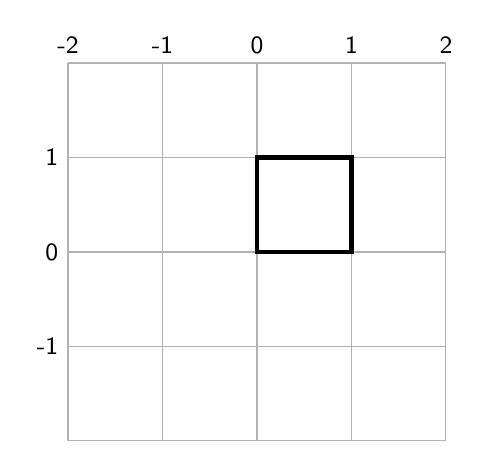
\begin{tikzpicture}[scale=1.2]
        % Draw the background grid: 4 columns (x=-2 to 2) and 3 rows (y=-2 to 1)
        \draw[thin, gray!60] (-2,-2) grid (2,2);
        
        % Horizontal/X-axis labels at the top of each vertical line
        \node[above, font=\small\sffamily] at (-2,2) {-2};
        \node[above, font=\small\sffamily] at (-1,2) {-1};
        \node[above, font=\small\sffamily] at (0,2) {0};
        \node[above, font=\small\sffamily] at (1,2) {1};
        \node[above, font=\small\sffamily] at (2,2) {2};
        
        % Vertical/Y-axis labels next to their respective horizontal lines
        \node[left, font=\small\sffamily] at (-2,1) {1};
        \node[left, font=\small\sffamily] at (-2,0) {0};
        \node[left, font=\small\sffamily] at (-2,-1) {-1};
        
        % Draw the bolded square from (0,0) to (1,1)
        \draw[ultra thick, black] (0,0) rectangle (1,1);
    \end{tikzpicture}
    
    \vspace{0.4cm}
    \flushleft
    View 1: Square with vertices $(0, 0, 0)$, $(1, 0, 0)$, $(1, 1, 0)$, and $(0, 1, 0)$.
  \end{center}


%% ─────────────────────────────────────────────────────────────────────
%% Q21. Square: coordinate matrix, scale (-3/2, 1/2), rotate -60 about z
%% ─────────────────────────────────────────────────────────────────────
\begin{tcolorbox}[enhanced,breakable,
  colback=cF!4,colframe=cF,boxrule=0.8pt,arc=5pt,
  title={\textbf{Answer --- Square: Coordinate Matrix, Scaling, Rotation by $-60^\circ$ about $z$}},
  fonttitle=\bfseries\color{white},colbacktitle=cF]

\textbf{(i) Coordinate matrix of the square.}

Vertices: $(0,0,0)$, $(1,0,0)$, $(1,1,0)$, $(0,1,0)$. Each column is a vertex:
\[
M=\begin{pmatrix}0&1&1&0\\0&0&1&1\\0&0&0&0\end{pmatrix}.
\]

\textbf{(ii) Scale by $-\tfrac{3}{2}$ in $x$, $\tfrac{1}{2}$ in $y$, $1$ in $z$.}

Scaling matrix:
\[
S=\begin{pmatrix}-\frac{3}{2}&0&0\\0&\frac{1}{2}&0\\0&0&1\end{pmatrix}.
\]
Scaled vertices:
\[
SM=\begin{pmatrix}0&-\frac{3}{2}&-\frac{3}{2}&0\\0&0&\frac{1}{2}&\frac{1}{2}\\0&0&0&0\end{pmatrix}.
\]

\textbf{(iii) Rotate by $-60^\circ$ about the $z$-axis.}

\[
R_z(-60^\circ)=\begin{pmatrix}\frac{1}{2}&\frac{\sqrt{3}}{2}&0\\-\frac{\sqrt{3}}{2}&\frac{1}{2}&0\\0&0&1\end{pmatrix}.
\]

Final image vertices $R_z(-60^\circ)\cdot SM$:
\[
\text{Vertex 1: }(0,0,0),\quad
\text{Vertex 2: }\left(-\frac{3}{4},\frac{3\sqrt{3}}{4},0\right),
\]
\[
\text{Vertex 3: }\left(-\frac{3}{4}+\frac{\sqrt{3}}{4},\;\frac{3\sqrt{3}}{4}+\frac{1}{4},\;0\right),\quad
\text{Vertex 4: }\left(\frac{\sqrt{3}}{4},\;\frac{1}{4},\;0\right).
\]

\end{tcolorbox}

\Q{Find the standard matrix for the transformation $T$ on $\mathbb{R}^3$, where $T$ is the composition of a rotation of $-30^\circ$ about the $x$-axis, followed by a contraction with factor $\frac{1}{4}$, followed by a reflection about the $yz$-plane, followed by an orthogonal projection on the $xz$-plane.
\yr{MATH 259 | L-2/T-1 | 2021-22} \mk{15}}

%% ─────────────────────────────────────────────────────────────────────
%% Q: Rot-30x -> Contraction 1/4 -> Reflect yz -> Project xz
%% ─────────────────────────────────────────────────────────────────────
\begin{tcolorbox}[enhanced,breakable,
  colback=cF!4,colframe=cF,boxrule=0.8pt,arc=5pt,
  title={\textbf{Answer --- Composition: Rot$(-30^\circ,x)$ $\to$ Contract$(\frac{1}{4})$ $\to$ Reflect$(yz)$ $\to$ Project$(xz)$}},
  fonttitle=\bfseries\color{white},colbacktitle=cF]

\textbf{Standard matrices for each operation:}

\textit{(1) Rotation by $-30^\circ$ about $x$-axis:}
\[
A_1=R_x(-30^\circ)=\begin{pmatrix}1&0&0\\0&\frac{\sqrt{3}}{2}&\frac{1}{2}\\0&-\frac{1}{2}&\frac{\sqrt{3}}{2}\end{pmatrix}.
\]

\textit{(2) Contraction with factor $k=\frac{1}{4}$:}
$A_2=\frac{1}{4}I$.

\textit{(3) Reflection about $yz$-plane ($x\mapsto-x$):}
$A_3=\begin{pmatrix}-1&0&0\\0&1&0\\0&0&1\end{pmatrix}$.

\textit{(4) Projection onto $xz$-plane ($y\mapsto 0$):}
$A_4=\begin{pmatrix}1&0&0\\0&0&0\\0&0&1\end{pmatrix}$.

\textbf{Composition} $A=A_4A_3A_2A_1$:
\[
A_2A_1=\frac{1}{4}R_x(-30^\circ)=\begin{pmatrix}\frac{1}{4}&0&0\\0&\frac{\sqrt{3}}{8}&\frac{1}{8}\\0&-\frac{1}{8}&\frac{\sqrt{3}}{8}\end{pmatrix}.
\]
\[
A_3(A_2A_1)=\begin{pmatrix}-\frac{1}{4}&0&0\\0&\frac{\sqrt{3}}{8}&\frac{1}{8}\\0&-\frac{1}{8}&\frac{\sqrt{3}}{8}\end{pmatrix}.
\]
\[
A=A_4\cdot(A_3A_2A_1)=\begin{pmatrix}-\frac{1}{4}&0&0\\0&0&0\\0&-\frac{1}{8}&\frac{\sqrt{3}}{8}\end{pmatrix}.
\]

\textit{Check:} The zero middle row confirms all output $y$-components are 0 (projection onto $xz$-plane).

\end{tcolorbox}

\Q{Describe the geometric effect of multiplying a vector $x$ by $A = \begin{pmatrix} \frac{\sqrt{3}}{2} & -\frac{1}{2} \\ \frac{1}{2} & \frac{\sqrt{3}}{2} \end{pmatrix}$.
\yr{MATH 259 | L-2/T-1 | 2020-21} \mk{10}}


%% ─────────────────────────────────────────────────────────────────────
%% Q14. Geometric effect of A=[[sqrt3/2,-1/2],[1/2,sqrt3/2]]
%% ─────────────────────────────────────────────────────────────────────
\begin{tcolorbox}[enhanced,breakable,
  colback=cF!4,colframe=cF,boxrule=0.8pt,arc=5pt,
  title={\textbf{Answer --- Geometric Effect of $A=\begin{pmatrix}\frac{\sqrt{3}}{2}&-\frac{1}{2}\\[3pt]\frac{1}{2}&\frac{\sqrt{3}}{2}\end{pmatrix}$}},
  fonttitle=\bfseries\color{white},colbacktitle=cF]

\textbf{Recognition:} Compare with the standard rotation matrix in $\mathbb{R}^2$:
\[
R_\theta=\begin{pmatrix}\cos\theta&-\sin\theta\\\sin\theta&\cos\theta\end{pmatrix}.
\]

Matching entries: $\cos\theta=\dfrac{\sqrt{3}}{2}$ and $\sin\theta=\dfrac{1}{2}$.

This gives $\theta=30^\circ=\dfrac{\pi}{6}$.

\textbf{Verification:}
\begin{itemize}[itemsep=2pt]
  \item $\det(A)=\dfrac{\sqrt{3}}{2}\cdot\dfrac{\sqrt{3}}{2}+\dfrac{1}{2}\cdot\dfrac{1}{2}=\dfrac{3}{4}+\dfrac{1}{4}=1$. (Rotations have determinant 1.) \checkmark
  \item $A^TA=I$. (Rotation matrices are orthogonal.) \checkmark
  \item Eigenvalues of $A$ are $e^{\pm i\pi/6}$ (complex, confirming a rotation with no real fixed direction). \checkmark
\end{itemize}

\textbf{Geometric effect:} Multiplying by $A$ is a \textbf{counterclockwise rotation by $30^\circ$} about the origin in $\mathbb{R}^2$. Lengths are preserved ($\|A\mathbf{x}\|=\|\mathbf{x}\|$), and all angles between vectors are preserved.

\end{tcolorbox}

\Q{Determine whether $T: M_{nn} \to \mathbb{R}$, where $T(A) = \mathrm{tr}(A)$, is a linear transformation.
\yr{MATH 259 | L-2/T-1 | 2020-21} \mk{10}}

%% ─────────────────────────────────────────────────────────────────────
%% Q15. T(A) = tr(A): Is T:M_nn->R linear?
%% ─────────────────────────────────────────────────────────────────────
\begin{tcolorbox}[enhanced,breakable,
  colback=cF!4,colframe=cF,boxrule=0.8pt,arc=5pt,
  title={\textbf{Answer --- $T(A)=\mathrm{tr}(A)$: Is $T:M_{nn}\to\mathbb{R}$ Linear?}},
  fonttitle=\bfseries\color{white},colbacktitle=cF]

\textbf{Yes, $T$ is a linear transformation.}

\textbf{Proof.} Let $A,B\in M_{nn}$ and $c\in\mathbb{R}$.

\textbf{(i) Additivity:}
\[
T(A+B)=\mathrm{tr}(A+B)=\sum_{i=1}^n(a_{ii}+b_{ii})=\sum_{i=1}^n a_{ii}+\sum_{i=1}^n b_{ii}=\mathrm{tr}(A)+\mathrm{tr}(B)=T(A)+T(B).\;\checkmark
\]

\textbf{(ii) Homogeneity:}
\[
T(cA)=\mathrm{tr}(cA)=\sum_{i=1}^n(ca_{ii})=c\sum_{i=1}^n a_{ii}=c\,\mathrm{tr}(A)=cT(A).\;\checkmark
\]

Since both properties hold, $T$ is linear.

\medskip\textit{Remark:} The trace functional is one of the most important linear maps in matrix theory. Its kernel consists of all \textbf{traceless matrices} (matrices with $\mathrm{tr}(A)=0$), which form a subspace of dimension $n^2-1$.

\end{tcolorbox}

\Q{Describe the kernel and range of the orthogonal projection on the plane $y = x$.
\yr{MATH 259 | L-2/T-1 | 2020-21} \mk{10}
\variant{MATH 247 | 2018-19; MATH 143 | 2021-22}}


%% ─────────────────────────────────────────────────────────────────────
%% Q16. Kernel and range of orthogonal projection on plane y=x (in R^3)
%% ─────────────────────────────────────────────────────────────────────
\begin{tcolorbox}[enhanced,breakable,
  colback=cF!4,colframe=cF,boxrule=0.8pt,arc=5pt,
  title={\textbf{Answer --- Kernel \& Range of Projection onto Plane $y=x$ in $\mathbb{R}^3$}},
  fonttitle=\bfseries\color{white},colbacktitle=cF]

The plane $y=x$ in $\mathbb{R}^3$ can be described as $\{(x,y,z)\mid y-x=0\}$. Its normal vector is $\mathbf{n}=(-1,1,0)/\sqrt{2}$.

\textbf{Projection matrix:}
\[
P=I-\mathbf{n}\mathbf{n}^T=I-\frac{1}{2}\begin{pmatrix}-1\\1\\0\end{pmatrix}\begin{pmatrix}-1&1&0\end{pmatrix}
=\begin{pmatrix}1&0&0\\0&1&0\\0&0&1\end{pmatrix}-\frac{1}{2}\begin{pmatrix}1&-1&0\\-1&1&0\\0&0&0\end{pmatrix}
=\begin{pmatrix}\frac{1}{2}&\frac{1}{2}&0\\[4pt]\frac{1}{2}&\frac{1}{2}&0\\0&0&1\end{pmatrix}.
\]

\textbf{Kernel of $T$:} The kernel consists of vectors that project to $\mathbf{0}$, i.e.\ vectors \emph{normal} to the plane:
\[
\ker(T)=\mathrm{span}\!\left\{(-1,1,0)^T\right\},\quad\dim(\ker T)=1.
\]
\textit{Verification:} $P(-1,1,0)^T=(-\tfrac{1}{2}+\tfrac{1}{2},\tfrac{1}{2}-\tfrac{1}{2},0)^T=(0,0,0)^T$. \checkmark

\textbf{Range of $T$:} The range is the plane $y=x$ itself. A basis for this plane:
\[
\mathrm{Range}(T)=\mathrm{span}\!\left\{(1,1,0)^T,(0,0,1)^T\right\},\quad\dim(\mathrm{Range})=2.
\]
\textit{Verification:} $P(1,1,0)^T=(\tfrac{1}{2}+\tfrac{1}{2},\tfrac{1}{2}+\tfrac{1}{2},0)^T=(1,1,0)^T$ \checkmark and $P(0,0,1)^T=(0,0,1)^T$ \checkmark (both already in the plane).

\textbf{Rank-Nullity:} $\dim(\ker)+\dim(\mathrm{Range})=1+2=3$. \checkmark

\end{tcolorbox}

\Q{Find the standard matrix for the composition $T$ on $\mathbb{R}^3$: rotation of $60^\circ$ about the $z$-axis, followed by a reflection about the $xy$-plane, followed by a contraction with factor $k = \frac{1}{2}$. Find the image of $(2,1,-1)$ and explain geometrically.
\yr{MATH 247 | L-2/T-2 | 2020-21} \mk{16}}


%% ─────────────────────────────────────────────────────────────────────
%% Q28. Rot 60 about z -> Reflect xy -> Contraction k=1/2. Find T(2,1,-1).
%% ─────────────────────────────────────────────────────────────────────
%% ─────────────────────────────────────────────────────────────────────
%% CORRECTED Q28. Rot 60 about z -> Reflect xy -> Contraction k=1/2.
%% ─────────────────────────────────────────────────────────────────────
\begin{tcolorbox}[enhanced,breakable,
  colback=cF!4,colframe=cF,boxrule=0.8pt,arc=5pt,
  title={\textbf{Answer --- Composition: Rot$(60^\circ,z)$ $\to$ Reflect$(xy)$ $\to$ Contraction$(\frac{1}{2})$; $T(2,1,-1)$}},
  fonttitle=\bfseries\color{white},colbacktitle=cF]

\textbf{Step 1: Standard matrices.}

\textit{Rotation by $60^\circ$ about the $z$-axis:}
\[
A_1=R_z(60^\circ)=\begin{pmatrix}\frac{1}{2}&-\frac{\sqrt{3}}{2}&0\\\frac{\sqrt{3}}{2}&\frac{1}{2}&0\\0&0&1\end{pmatrix}.
\]

\textit{Reflection about $xy$-plane} ($z\mapsto -z$):
\[
A_2=\begin{pmatrix}1&0&0\\0&1&0\\0&0&-1\end{pmatrix}.
\]

\textit{Contraction by $k=\tfrac{1}{2}$:}
\[
A_3=\frac{1}{2}I.
\]

\textbf{Step 2: Composition} $A=\frac{1}{2}\cdot R_{xy}\cdot R_z(60^\circ)$:

\[
A_2A_1=\begin{pmatrix}\frac{1}{2}&-\frac{\sqrt{3}}{2}&0\\\frac{\sqrt{3}}{2}&\frac{1}{2}&0\\0&0&-1\end{pmatrix},
\qquad
A=\frac{1}{2}A_2A_1=\begin{pmatrix}\frac{1}{4}&-\frac{\sqrt{3}}{4}&0\\[4pt]\frac{\sqrt{3}}{4}&\frac{1}{4}&0\\0&0&-\frac{1}{2}\end{pmatrix}.
\]

\textbf{Step 3: Compute $T(2,1,-1)$:}
\[
A\begin{pmatrix}2\\1\\-1\end{pmatrix}=\begin{pmatrix}\frac{2}{4}-\frac{\sqrt{3}}{4}\\\frac{2\sqrt{3}}{4}+\frac{1}{4}\\\frac{1}{2}\end{pmatrix}=\boxed{\begin{pmatrix}\frac{2-\sqrt{3}}{4}\\[4pt]\frac{2\sqrt{3}+1}{4}\\[4pt]\frac{1}{2}\end{pmatrix}}.
\]

\textbf{Geometric interpretation:} The operator first rotates counterclockwise by $60^\circ$ in the $xy$-plane, then flips the $z$-component, then uniformly halves all distances from the origin (contraction). The combined operator \textbf{is one-to-one} because $\det(A) = \left(\tfrac{1}{2}\right)^3\cdot(-1)\cdot 1 = -\tfrac{1}{8} \neq 0$. The negative determinant indicates an orientation reversal, while the fractional magnitude indicates the volume of the space is contracted.

\end{tcolorbox}

\Q{Let $T_1(x_1,x_2,x_3) = (4x_1, -2x_1+x_2, -x_1-3x_2)$ and $T_2(x_1,x_2,x_3) = (x_1+2x_2, -x_3, 4x_1-x_3)$. Find the standard matrices for $T_1$ and $T_2$. Also find $T_2 \circ T_1$ and $T_1 \circ T_2$.
\yr{MATH 247 | L-2/T-2 | 2020-21} \mk{14.67}}


%% ─────────────────────────────────────────────────────────────────────
%% Q29. T1(x1,x2,x3)=(4x1,-2x1+x2,-x1-3x2) and T2(x1,x2,x3)=(x1+2x2,-x3,4x1-x3).
%%      Standard matrices + T2∘T1 and T1∘T2.
%% ─────────────────────────────────────────────────────────────────────
\begin{tcolorbox}[enhanced,breakable,
  colback=cF!4,colframe=cF,boxrule=0.8pt,arc=5pt,
  title={\textbf{Answer --- Standard Matrices of $T_1$, $T_2$; Compositions $T_2\circ T_1$ and $T_1\circ T_2$}},
  fonttitle=\bfseries\color{white},colbacktitle=cF]

\textbf{Standard matrix of $T_1$:}
$T_1(x_1,x_2,x_3)=(4x_1,\;-2x_1+x_2,\;-x_1-3x_2)$.

The columns of $A_1$ are $T_1(e_1)$, $T_1(e_2)$, $T_1(e_3)$:
\[
T_1(1,0,0)=(4,-2,-1),\quad T_1(0,1,0)=(0,1,-3),\quad T_1(0,0,1)=(0,0,0).
\]
\[
A_1=\begin{pmatrix}4&0&0\\-2&1&0\\-1&-3&0\end{pmatrix}.
\]

\textbf{Standard matrix of $T_2$:}
$T_2(x_1,x_2,x_3)=(x_1+2x_2,\;-x_3,\;4x_1-x_3)$.
\[
T_2(1,0,0)=(1,0,4),\quad T_2(0,1,0)=(2,0,0),\quad T_2(0,0,1)=(0,-1,-1).
\]
\[
A_2=\begin{pmatrix}1&2&0\\0&0&-1\\4&0&-1\end{pmatrix}.
\]

\textbf{Composition $T_2\circ T_1$} (apply $T_1$ first, then $T_2$): matrix is $A_2A_1$:
\[
A_2A_1=\begin{pmatrix}1&2&0\\0&0&-1\\4&0&-1\end{pmatrix}\begin{pmatrix}4&0&0\\-2&1&0\\-1&-3&0\end{pmatrix}=\begin{pmatrix}0&2&0\\1&3&0\\17&3&0\end{pmatrix}.
\]

Formula: $(T_2\circ T_1)(x_1,x_2,x_3)=(2x_2,\;x_1+3x_2,\;17x_1+3x_2)$.

\textbf{Composition $T_1\circ T_2$} (apply $T_2$ first, then $T_1$): matrix is $A_1A_2$:
\[
A_1A_2=\begin{pmatrix}4&0&0\\-2&1&0\\-1&-3&0\end{pmatrix}\begin{pmatrix}1&2&0\\0&0&-1\\4&0&-1\end{pmatrix}=\begin{pmatrix}4&8&0\\-2&-4&-1\\-1&-2&3\end{pmatrix}.
\]

Formula: $(T_1\circ T_2)(x_1,x_2,x_3)=(4x_1+8x_2,\;-2x_1-4x_2-x_3,\;-x_1-2x_2+3x_3)$.

\textit{Note:} $T_2\circ T_1\neq T_1\circ T_2$ in general, confirming that composition of linear transformations is not commutative.

\end{tcolorbox}

\Q{Find the standard matrix for $T$ on $\mathbb{R}^3$, where $T$ is a rotation of $60^\circ$ about the $y$-axis, followed by a reflection about the $yz$-plane, followed by a dilation with factor $k = 2$. Find $T(2,-1,4)$.
\yr{MATH 247 | L-2/T-2 | 2019-20} \mk{16.67}}

%% ─────────────────────────────────────────────────────────────────────
%% Q26. Rot 60 about y -> Reflect yz -> Dilation k=2. Find T(2,-1,4).
%% ─────────────────────────────────────────────────────────────────────
\begin{tcolorbox}[enhanced,breakable,
  colback=cF!4,colframe=cF,boxrule=0.8pt,arc=5pt,
  title={\textbf{Answer --- Composition: Rot$(60^\circ,y)$ $\to$ Reflect$(yz)$ $\to$ Dilation$(2)$; $T(2,-1,4)$}},
  fonttitle=\bfseries\color{white},colbacktitle=cF]

\textbf{Step 1: Standard matrices.}

\[
A_1=R_y(60^\circ)=\begin{pmatrix}\frac{1}{2}&0&\frac{\sqrt{3}}{2}\\0&1&0\\-\frac{\sqrt{3}}{2}&0&\frac{1}{2}\end{pmatrix},\quad
A_2=R_{yz}=\begin{pmatrix}-1&0&0\\0&1&0\\0&0&1\end{pmatrix},\quad
A_3=2I.
\]

\textbf{Step 2: Composition} $A=2R_{yz}R_y(60^\circ)$:

\[
R_{yz}A_1=\begin{pmatrix}-\frac{1}{2}&0&-\frac{\sqrt{3}}{2}\\0&1&0\\-\frac{\sqrt{3}}{2}&0&\frac{1}{2}\end{pmatrix},
\qquad
A=2(R_{yz}A_1)=\begin{pmatrix}-1&0&-\sqrt{3}\\0&2&0\\-\sqrt{3}&0&1\end{pmatrix}.
\]

\textbf{Step 3: Compute $T(2,-1,4)$:}
\[
A\begin{pmatrix}2\\-1\\4\end{pmatrix}=\begin{pmatrix}-2-4\sqrt{3}\\-2\\-2\sqrt{3}+4\end{pmatrix}=\boxed{\begin{pmatrix}-2-4\sqrt{3}\\-2\\4-2\sqrt{3}\end{pmatrix}}.
\]

Numerically: $-2-4\sqrt{3}\approx-8.93$, $4-2\sqrt{3}\approx0.54$.

\end{tcolorbox}

\Q{Let $T: \mathbb{R}^4 \to \mathbb{R}^3$ defined by $T(x,y,z,t) = (x-y+z+t,\; x+2z-t,\; x+y+3z-3t)$. Find basis and dimension of $\mathrm{Range}(T)$ and $\ker(T)$.
\yr{MATH 247 | L-2/T-2 | 2019-20} \mk{16.67}
\variant{MATH 243 | 2010-11; MATH 247 | 2018-19}}


%% ─────────────────────────────────────────────────────────────────────
%% Q27. T:R^4->R^3, T(x,y,z,t)=(x-y+z+t, x+2z-t, x+y+3z-3t). ker, Range.
%%      (Same as Q22 but asked in MATH 247 context)
%% ─────────────────────────────────────────────────────────────────────
%% ─────────────────────────────────────────────────────────────────────
%% CORRECTED Q27. T:R^4->R^3, T(x,y,z,t)=(x-y+z+t, x+2z-t, x+y+3z-3t).
%% ─────────────────────────────────────────────────────────────────────
\begin{tcolorbox}[enhanced,breakable,
  colback=cF!4,colframe=cF,boxrule=0.8pt,arc=5pt,
  title={\textbf{Answer --- $T:\mathbb{R}^4\to\mathbb{R}^3$ (MATH 247): $\ker T$ and $\mathrm{Range}(T)$}},
  fonttitle=\bfseries\color{white},colbacktitle=cF]

\textbf{Step 1: Write the standard matrix $A$.}

Extract the coefficients from $T(x,y,z,t) = (x-y+z+t,\; x+2z-t,\; x+y+3z-3t)$:
\[
A=\begin{pmatrix}1&-1&1&1\\1&0&2&-1\\1&1&3&-3\end{pmatrix}.
\]

\textbf{Step 2: Row-reduce $A$ to find the pivot columns.}

\[
\begin{pmatrix}1&-1&1&1\\1&0&2&-1\\1&1&3&-3\end{pmatrix}
\xrightarrow{\substack{R_2-R_1\\[1pt] R_3-R_1}}
\begin{pmatrix}1&-1&1&1\\0&1&1&-2\\0&2&2&-4\end{pmatrix}
\xrightarrow{R_3-2R_2}
\begin{pmatrix}1&-1&1&1\\0&1&1&-2\\0&0&0&0\end{pmatrix}
\]
\[
\xrightarrow{R_1+R_2}
\begin{pmatrix}1&0&2&-1\\0&1&1&-2\\0&0&0&0\end{pmatrix}.
\]

Pivot columns are 1 and 2. $\mathrm{rank}(A)=2$.

\medskip\textbf{Range of $T$:}
Formed by the corresponding pivot columns of the \emph{original} matrix $A$:
\[
\boxed{\mathrm{Range}(T)=\mathrm{span}\!\left\{\begin{pmatrix}1\\1\\1\end{pmatrix},\;\begin{pmatrix}-1\\0\\1\end{pmatrix}\right\},\quad\dim(\mathrm{Range})=2.}
\]

\medskip\textbf{Kernel of $T$:}
From the RREF, the free variables are $z$ and $t$.
\[
x + 2z - t = 0 \implies x = -2z + t
\]
\[
y + z - 2t = 0 \implies y = -z + 2t
\]
Setting $z=1, t=0$ yields $(-2,-1,1,0)^T$. Setting $z=0, t=1$ yields $(1,2,0,1)^T$.
\[
\boxed{\ker(T)=\mathrm{span}\!\left\{\begin{pmatrix}-2\\-1\\1\\0\end{pmatrix},\;\begin{pmatrix}1\\2\\0\\1\end{pmatrix}\right\},\quad\dim(\ker T)=2.}
\]

\textbf{Rank-Nullity check:} $2+2=4=\dim(\mathbb{R}^4)$. \checkmark

\end{tcolorbox}


\Q{Determine whether $T(x,y,s,t) = (4x+y-2s-3t,\; 2x+y+s-4t,\; 6x-9s+9t)$ is a linear operator. Find basis and dimension of $\ker T$ and $\mathrm{Range}\,T$.
\yr{MATH 259 | L-2/T-1 | 2018-19} \mk{20}
\variant{MATH 259 | 2014-15, 2021-22; MATH 143 | 2022-23}}


%% ─────────────────────────────────────────────────────────────────────
%% Q10. T(x,y,s,t)=(4x+y-2s-3t, 2x+y+s-4t, 6x-9s+9t): ker, Range
%% ─────────────────────────────────────────────────────────────────────
\begin{tcolorbox}[enhanced,breakable,
  colback=cF!4,colframe=cF,boxrule=0.8pt,arc=5pt,
  title={\textbf{Answer --- $T:\mathbb{R}^4\to\mathbb{R}^3$, $T(x,y,s,t)=(\ldots)$; Kernel \& Range}},
  fonttitle=\bfseries\color{white},colbacktitle=cF]

Standard matrix:
\[
A=\begin{pmatrix}4&1&-2&-3\\2&1&1&-4\\6&0&-9&9\end{pmatrix}.
\]

\textbf{Since $T(\mathbf{x})=A\mathbf{x}$, it is linear by definition.}

\textbf{Step 1: Row-reduce $A$.}
\[
\begin{pmatrix}4&1&-2&-3\\2&1&1&-4\\6&0&-9&9\end{pmatrix}
\xrightarrow{\text{operations}}
\begin{pmatrix}1&0&-\frac{3}{2}&0\\0&1&4&0\\0&0&0&1\end{pmatrix}.
\]

Pivot columns: 1, 2, 4. $\mathrm{rank}(A)=3$.

\medskip\textbf{Step 2: Kernel of $T$ (null space).}

Free variable: $s=t$. From RREF: $x=\tfrac{3s}{2}$, $y=-4s$, $t=0$. With $s=2$ (to clear fractions):
\[
\boxed{\ker(T)=\mathrm{span}\!\left\{\begin{pmatrix}3\\-8\\2\\0\end{pmatrix}\right\},\quad\dim(\ker T)=1.}
\]

\textit{Alternatively $\ker(T)=\mathrm{span}\{(3,-8,2,0)^T\}$ or scaled as $(\tfrac{3}{2},-4,1,0)^T$.}

\medskip\textbf{Step 3: Range of $T$ (column space).}

Pivot columns 1, 2, 4 of the original $A$:
\[
\boxed{\mathrm{Range}(T)=\mathrm{span}\!\left\{\begin{pmatrix}4\\2\\6\end{pmatrix},\;\begin{pmatrix}1\\1\\0\end{pmatrix},\;\begin{pmatrix}-3\\-4\\9\end{pmatrix}\right\},\quad\dim(\mathrm{Range})=3.}
\]

\textbf{Rank-Nullity check:} $3+1=4$. \checkmark

\end{tcolorbox}

\Q{Let $T: P_2 \to P_3$ be the linear transformation $T(p(x)) = x p(3x-5)$. Find the matrix for $T$ with respect to the standard bases $B = \{1,x,x^2\}$ and $B' = \{1,x,x^2,x^3\}$. Verify $[T]_{B',B}[x]_B = [T(x)]_{B'}$.
\yr{MATH 259 | L-2/T-1 | 2018-19} \mk{15}
\variant{MATH 215 | 2016-17}}


%% ─────────────────────────────────────────────────────────────────────
%% Q11. T:P2->P3, T(p(x))=x*p(3x-5). Matrix + verify A[p]_B=[T(p)]_{B'}
%% ─────────────────────────────────────────────────────────────────────
\begin{tcolorbox}[enhanced,breakable,
  colback=cF!4,colframe=cF,boxrule=0.8pt,arc=5pt,
  title={\textbf{Answer --- $T:P_2\to P_3$, $T(p(x))=xp(3x-5)$; Matrix \& Verification}},
  fonttitle=\bfseries\color{white},colbacktitle=cF]

\textit{Same transformation as Q3. The matrix is:}

\[
[T]_{B',B}=\begin{pmatrix}0&0&0\\1&-5&25\\0&3&-30\\0&0&9\end{pmatrix},\quad B=\{1,x,x^2\},\quad B'=\{1,x,x^2,x^3\}.
\]

\textbf{Verify $A[x]_B=[T(x)]_{B'}$} (using $p(x)=x$, so $[x]_B=(0,1,0)^T$):

\[
[T]_{B',B}\begin{pmatrix}0\\1\\0\end{pmatrix}=\begin{pmatrix}0\\1\cdot0+(-5)\cdot1+25\cdot0\\0\cdot0+3\cdot1+(-30)\cdot0\\0\end{pmatrix}=\begin{pmatrix}0\\-5\\3\\0\end{pmatrix}.
\]

Meanwhile, $T(x)=x\cdot(3x-5)=3x^2-5x$, and $[3x^2-5x]_{B'}=(0,-5,3,0)^T$.\;\checkmark

The relation $A[\mathbf{p}]_B=[T(\mathbf{p})]_{B'}$ holds for any $\mathbf{p}\in P_2$.

\end{tcolorbox}

\Q{Find the standard matrix for $T$ on $\mathbb{R}^3$, where $T$ is the composition of a reflection about the $xy$-plane, followed by a reflection about the $xz$-plane, followed by an orthogonal projection on the $yz$-plane.
\yr{MATH 259 | L-2/T-1 | 2018-19} \mk{17}}

%% ─────────────────────────────────────────────────────────────────────
%% Q12. Composition: Reflect xy -> Reflect xz -> Project yz
%% ─────────────────────────────────────────────────────────────────────
\begin{tcolorbox}[enhanced,breakable,
  colback=cF!4,colframe=cF,boxrule=0.8pt,arc=5pt,
  title={\textbf{Answer --- Composition: Reflect$(xy)$ $\to$ Reflect$(xz)$ $\to$ Project$(yz)$}},
  fonttitle=\bfseries\color{white},colbacktitle=cF]

\textbf{Standard matrices:}

\textit{Reflection about $xy$-plane} ($z\mapsto-z$):
$A_1=\begin{pmatrix}1&0&0\\0&1&0\\0&0&-1\end{pmatrix}$.

\textit{Reflection about $xz$-plane} ($y\mapsto-y$):
$A_2=\begin{pmatrix}1&0&0\\0&-1&0\\0&0&1\end{pmatrix}$.

\textit{Projection onto $yz$-plane} ($x\mapsto0$):
$A_3=\begin{pmatrix}0&0&0\\0&1&0\\0&0&1\end{pmatrix}$.

\textbf{Composition} $A=A_3A_2A_1$:

\[
A_2A_1=\begin{pmatrix}1&0&0\\0&-1&0\\0&0&-1\end{pmatrix},
\qquad
A=P_{yz}(A_2A_1)=\begin{pmatrix}0&0&0\\0&-1&0\\0&0&-1\end{pmatrix}.
\]

\textbf{Interpretation:} The combined effect projects onto the $yz$-plane, then negates both $y$ and $z$. The $x$-component is lost (projection), while $y$ and $z$ are flipped by the two reflections.

\end{tcolorbox}


\Q{Determine whether the linear operator $T: \mathbb{R}^3 \to \mathbb{R}^3$ defined by $w_1 = x_1 + 4x_2 - x_3$, $w_2 = 2x_1 + 7x_2 + x_3$, $w_3 = x_1 + 3x_2$ is one-to-one. If so, find the standard matrix for the inverse operator and find $T^{-1}$.
\yr{MATH 259 | L-2/T-1 | 2018-19} \mk{18}}

%% ─────────────────────────────────────────────────────────────────────
%% Q13. T:R^3->R^3, w1=x1+4x2-x3, w2=2x1+7x2+x3, w3=x1+3x2.
%%     One-to-one? T^-1?
%% ─────────────────────────────────────────────────────────────────────
\begin{tcolorbox}[enhanced,breakable,
  colback=cF!4,colframe=cF,boxrule=0.8pt,arc=5pt,
  title={\textbf{Answer --- $T:\mathbb{R}^3\to\mathbb{R}^3$ (given by $w_i$): One-to-One? Inverse?}},
  fonttitle=\bfseries\color{white},colbacktitle=cF]

\textbf{Standard matrix:}
\[
A=\begin{pmatrix}1&4&-1\\2&7&1\\1&3&0\end{pmatrix}.
\]

\textbf{Is $T$ one-to-one?} Compute $\det(A)$:
\[
\det(A)=1(7\cdot0-1\cdot3)-4(2\cdot0-1\cdot1)+(-1)(2\cdot3-7\cdot1)=1(-3)-4(-1)-1(-1)
\]
\[
=-3+4+1=2\neq0.
\]

Since $\det(A)=2\neq0$, $T$ is \textbf{one-to-one} (and onto). $T$ is invertible.

\medskip\textbf{Standard matrix of $T^{-1}$:} Compute $A^{-1}$ by row reduction on $[A\mid I]$:

\[
[A\mid I]=\left[\begin{array}{ccc|ccc}1&4&-1&1&0&0\\2&7&1&0&1&0\\1&3&0&0&0&1\end{array}\right]
\xrightarrow{R_2-2R_1,\;R_3-R_1}
\left[\begin{array}{ccc|ccc}1&4&-1&1&0&0\\0&-1&3&-2&1&0\\0&-1&1&-1&0&1\end{array}\right]
\]
\[
\xrightarrow{-R_2,\;R_3-R_2}
\left[\begin{array}{ccc|ccc}1&4&-1&1&0&0\\0&1&-3&2&-1&0\\0&0&-2&1&-1&1\end{array}\right]
\xrightarrow{-\frac{1}{2}R_3}
\left[\begin{array}{ccc|ccc}1&4&-1&1&0&0\\0&1&-3&2&-1&0\\0&0&1&-\frac{1}{2}&\frac{1}{2}&-\frac{1}{2}\end{array}\right]
\]
\[
\xrightarrow{\text{back-sub}}
A^{-1}=\begin{pmatrix}-\frac{3}{2}&-\frac{3}{2}&\frac{11}{2}\\[4pt]\frac{1}{2}&\frac{1}{2}&-\frac{3}{2}\\[4pt]-\frac{1}{2}&\frac{1}{2}&-\frac{1}{2}\end{pmatrix}.
\]

\textbf{Formula for $T^{-1}$:}
\[
T^{-1}(w_1,w_2,w_3)=\left(-\tfrac{3}{2}w_1-\tfrac{3}{2}w_2+\tfrac{11}{2}w_3,\;\tfrac{1}{2}w_1+\tfrac{1}{2}w_2-\tfrac{3}{2}w_3,\;-\tfrac{1}{2}w_1+\tfrac{1}{2}w_2-\tfrac{1}{2}w_3\right).
\]

\end{tcolorbox}


\Q{Consider the basis $S = \{v_1, v_2, v_3\}$ for $\mathbb{R}^3$, where $v_1 = (1,2,1)$, $v_2 = (2,9,0)$, $v_3 = (3,3,4)$. Let $T: \mathbb{R}^3 \to \mathbb{R}^2$ with $T(v_1) = (1,0)$, $T(v_2) = (-1,1)$, $T(v_3) = (0,1)$. Find a formula for $T(x,y,z)$ and compute $T(7,-3,5)$.
\yr{MATH 247 | L-2/T-2 | 2018-19} \mk{20}}

%% ─────────────────────────────────────────────────────────────────────
%% Q: T:R^3->R^2, basis S={v1=(1,2,1),v2=(2,9,0),v3=(3,3,4)}.
%%    T(v1)=(1,0), T(v2)=(-1,1), T(v3)=(0,1). Find formula, compute T(7,-3,5).
%% ─────────────────────────────────────────────────────────────────────
\begin{tcolorbox}[enhanced,breakable,
  colback=cF!4,colframe=cF,boxrule=0.8pt,arc=5pt,
  title={\textbf{Answer --- $T:\mathbb{R}^3\to\mathbb{R}^2$ from Basis Values; $T(7,-3,5)$}},
  fonttitle=\bfseries\color{white},colbacktitle=cF]

\textit{This uses the same basis $S$ as Q20. The standard matrix is the same:
$A_T=\begin{pmatrix}-41&9&24\\14&-3&-8\end{pmatrix}$.
(See Q20 for full derivation.)}

\textbf{Formula:} $T(x,y,z)=(-41x+9y+24z,\;14x-3y-8z)$.

\textbf{Compute $T(7,-3,5)$:}
\[
T(7,-3,5)=\begin{pmatrix}-41(7)+9(-3)+24(5)\\14(7)-3(-3)-8(5)\end{pmatrix}
=\begin{pmatrix}-287-27+120\\98+9-40\end{pmatrix}=\boxed{\begin{pmatrix}-194\\67\end{pmatrix}}.
\]

\end{tcolorbox}

\Q{Let the linear transformation be defined by $T(x,y,z) = (x-y-3z,\; 5x+6y-4z,\; 7x+4y+2z)$. Find (i) a basis and dimension of $\mathrm{Range}(T)$, (ii) a basis and dimension of $\ker(T)$. Verify the dimension theorem.
\yr{MATH 215 | L-2/T-2 | 2018-19} \mk{30}}

%% ─────────────────────────────────────────────────────────────────────
%% Q: T(x,y,z)=(x-y-3z,5x+6y-4z,7x+4y+2z). Range, ker, dim theorem.
%% ─────────────────────────────────────────────────────────────────────
\begin{tcolorbox}[enhanced,breakable,
  colback=cF!4,colframe=cF,boxrule=0.8pt,arc=5pt,
  title={\textbf{Answer --- $T(x,y,z)=(x-y-3z,\;5x+6y-4z,\;7x+4y+2z)$: Range, Kernel, Dimension Theorem}},
  fonttitle=\bfseries\color{white},colbacktitle=cF]

Standard matrix:
\[
A=\begin{pmatrix}1&-1&-3\\5&6&-4\\7&4&2\end{pmatrix}.
\]

\textbf{Step 1: Compute $\det(A)$.}
\[
\det(A)=1(12+16)+1(10+28)+(-3)(20-42)=28+38+66=132\neq0.
\]

Since $\det(A)\neq0$, $A$ is invertible and $\mathrm{rank}(A)=3$.

\textbf{Range of $T$:}

Since rank $=3=\dim(\mathbb{R}^3)$, the range of $T$ is all of $\mathbb{R}^3$:
\[
\boxed{\mathrm{Range}(T)=\mathbb{R}^3,\quad\dim(\mathrm{Range})=3.}
\]

A basis is any basis of $\mathbb{R}^3$, e.g.\ $\{(1,0,0)^T,(0,1,0)^T,(0,0,1)^T\}$.

\textbf{Kernel of $T$:}

Since $A$ is invertible, $A\mathbf{x}=\mathbf{0}$ has only the trivial solution:
\[
\boxed{\ker(T)=\{\mathbf{0}\},\quad\dim(\ker T)=0.}
\]

\textbf{Dimension Theorem verification:}
\[
\dim(\ker T)+\dim(\mathrm{Range}\,T)=0+3=3=\dim(\mathbb{R}^3).\;\checkmark
\]

\textit{Note}: Since $T$ is both one-to-one ($\ker=\{\mathbf{0}\}$) and onto ($\mathrm{Range}=\mathbb{R}^3$), $T$ is an \textbf{invertible} linear operator.

\end{tcolorbox}

\Q{Let $S = \{v_1, v_2, v_3\}$ be a basis for $P_2(x)$ where $v_1 = 1 + 2x + x^2$, $v_2 = 2 + 9x$, $v_3 = 3 + 3x + 4x^2$. Find the coordinate vector of $p(x) = 6 + 6x + 3x^2$ relative to $S$.
\yr{MATH 247 | 2018--19}}


%% ─────────────────────────────────────────────────────────────────────
%% Q: S={1+2x+x^2, 2+9x, 3+3x+4x^2} basis for P_2(x).
%%    Find coord vector of p(x)=6+6x+3x^2 relative to S.
%% ─────────────────────────────────────────────────────────────────────
\begin{tcolorbox}[enhanced,breakable,
  colback=cF!4,colframe=cF,boxrule=0.8pt,arc=5pt,
  title={\textbf{Answer --- Coordinate Vector of $6+6x+3x^2$ Relative to $S=\{v_1,v_2,v_3\}$}},
  fonttitle=\bfseries\color{white},colbacktitle=cF]

$v_1=1+2x+x^2$, $v_2=2+9x$, $v_3=3+3x+4x^2$. Find $c_1,c_2,c_3$ such that $c_1v_1+c_2v_2+c_3v_3=6+6x+3x^2$.

\textbf{Convert to coordinate system} $\{1,x,x^2\}$:
\[
c_1\begin{pmatrix}1\\2\\1\end{pmatrix}+c_2\begin{pmatrix}2\\9\\0\end{pmatrix}+c_3\begin{pmatrix}3\\3\\4\end{pmatrix}=\begin{pmatrix}6\\6\\3\end{pmatrix}.
\]

Row-reduce the augmented matrix:
\[
\left[\begin{array}{ccc|c}1&2&3&6\\2&9&3&6\\1&0&4&3\end{array}\right]
\xrightarrow{R_2-2R_1,\;R_3-R_1}
\left[\begin{array}{ccc|c}1&2&3&6\\0&5&-3&-6\\0&-2&1&-3\end{array}\right]
\xrightarrow{5R_3+2R_2}
\left[\begin{array}{ccc|c}1&2&3&6\\0&5&-3&-6\\0&0&-1&-27\end{array}\right].
\]

Back-substitute: $c_3=27$, $5c_2=3c_3-6=81-6=75\Rightarrow c_2=15$, $c_1=6-2(15)-3(27)=6-30-81=-105$.

\[
\boxed{[p]_S=\begin{pmatrix}-105\\15\\27\end{pmatrix}.}
\]

\textbf{Verification:}
$-105(1+2x+x^2)+15(2+9x)+27(3+3x+4x^2)$
$=(-105+30+81)+(-210+135+81)x+(-105+108)x^2$
$=6+6x+3x^2$. \checkmark

\end{tcolorbox}



\Q{Let $T: \mathbb{R}^4 \to \mathbb{R}^3$ be the linear transformation defined by $T(x,y,s,t) = (4x + y - 2s - 3t,\; 2x + y + s - 4t,\; 6x - 9s + 9t)$. Find a basis and the dimension of (i) the Kernel of $T$ and (ii) the Range of $T$.
\yr{MATH 259 | 2018--19, 2022--23 (BUET)}}


%% ─────────────────────────────────────────────────────────────────────
%% Q: T:R4->R3, T(x,y,s,t)=(4x+y-2s-3t,2x+y+s-4t,6x-9s+9t).
%%    Basis for ker(T) and range(T). [Same as Q10]
%% ─────────────────────────────────────────────────────────────────────
\begin{tcolorbox}[enhanced,breakable,
  colback=cF!4,colframe=cF,boxrule=0.8pt,arc=5pt,
  title={\textbf{Answer --- $T:\mathbb{R}^4\to\mathbb{R}^3$, $T(x,y,s,t)=(4x+y-2s-3t,\ldots)$: Kernel \& Range}},
  fonttitle=\bfseries\color{white},colbacktitle=cF]

\textit{This is identical to Q10. See Q10 for the full solution.}

\textbf{Summary:} Standard matrix $A=\begin{pmatrix}4&1&-2&-3\\2&1&1&-4\\6&0&-9&9\end{pmatrix}$, $\mathrm{rank}(A)=3$.

\[
\ker(T)=\mathrm{span}\!\left\{\begin{pmatrix}3\\-8\\2\\0\end{pmatrix}\right\},\quad\dim(\ker T)=1.
\]
\[
\mathrm{Range}(T)=\mathrm{span}\!\left\{\begin{pmatrix}4\\2\\6\end{pmatrix},\;\begin{pmatrix}1\\1\\0\end{pmatrix},\;\begin{pmatrix}-3\\-4\\9\end{pmatrix}\right\},\quad\dim(\mathrm{Range})=3.
\]

\end{tcolorbox}


\Q{Determine whether the linear operator $T: \mathbb{R}^3 \to \mathbb{R}^3$ defined by $w_1 = x_1 + 2x_2 + x_3$, $w_2 = -2x_1 + x_2 + 4x_3$, $w_3 = 7x_1 + 4x_2 - 5x_3$ is one-to-one. If so, find the inverse standard matrix and $T^{-1}$.
\yr{MATH 259 | L-2/T-1 | 2017-18} \mk{17}}

%% ─────────────────────────────────────────────────────────────────────
%% Q34. T: w1=x1+2x2+x3, w2=-2x1+x2+4x3, w3=7x1+4x2-5x3.
%%      One-to-one? If so, T^-1?
%% ─────────────────────────────────────────────────────────────────────
\begin{tcolorbox}[enhanced,breakable,
  colback=cF!4,colframe=cF,boxrule=0.8pt,arc=5pt,
  title={\textbf{Answer --- $T:\mathbb{R}^3\to\mathbb{R}^3$ (given by $w_i$): One-to-One?}},
  fonttitle=\bfseries\color{white},colbacktitle=cF]

\textbf{Standard matrix:}
\[
A=\begin{pmatrix}1&2&1\\-2&1&4\\7&4&-5\end{pmatrix}.
\]

\textbf{Compute $\det(A)$:}
\[
\det(A)=1(1\cdot(-5)-4\cdot4)-2((-2)(-5)-4\cdot7)+1((-2)\cdot4-1\cdot7)
\]
\[
=1(-5-16)-2(10-28)+1(-8-7)
=-21+36-15=0.
\]

Since $\det(A)=0$, $T$ is \textbf{not one-to-one} (singular matrix, non-trivial kernel).

\textbf{Finding the kernel:}
\[
\begin{pmatrix}1&2&1\\-2&1&4\\7&4&-5\end{pmatrix}
\xrightarrow{R_2+2R_1,\;R_3-7R_1}
\begin{pmatrix}1&2&1\\0&5&6\\0&-10&-12\end{pmatrix}
\xrightarrow{R_3+2R_2}
\begin{pmatrix}1&2&1\\0&5&6\\0&0&0\end{pmatrix}.
\]

Free variable $x_3=t$: $x_2=-\tfrac{6}{5}t$, $x_1=-2x_2-x_3=\tfrac{12}{5}t-t=\tfrac{7}{5}t$.

$\ker(T)=\mathrm{span}\{(7,-6,5)^T\}$, $\dim(\ker T)=1$.

Since the kernel is non-trivial, $T$ is \textbf{not invertible}.

\end{tcolorbox}

\Q{If $T: V \to W$ is a linear transformation, prove that (i) the kernel of $T$ is a subspace of $V$; (ii) the range of $T$ is a subspace of $W$.
\yr{MATH 247 | L-2/T-2 | 2017-18} \mk{16.67}}

%% ─────────────────────────────────────────────────────────────────────
%% Q: Kernel and Range of linear transformation T: V -> W
%% ─────────────────────────────────────────────────────────────────────
\begin{tcolorbox}[enhanced,breakable,colback=cF!4,colframe=cF,
  boxrule=0.8pt,arc=5pt,
  title={\textbf{Answer --- Kernel and Range of $T$ are Subspaces}},
  fonttitle=\bfseries\color{white},colbacktitle=cF]

\textbf{(i) $\ker(T)$ is a subspace of $V$.}

Let $T:V\to W$ be linear. $\ker(T)=\{v\in V: T(v)=0_W\}$.

\textbf{S1:} $T(0_V)=0_W$ (linearity), so $0_V\in\ker(T)$.\;\checkmark

\textbf{S2:} If $u,v\in\ker(T)$: $T(u+v)=T(u)+T(v)=0_W+0_W=0_W$, so $u+v\in\ker(T)$.\;\checkmark

\textbf{S3:} If $v\in\ker(T)$, $c\in\mathbb{R}$: $T(cv)=cT(v)=c\cdot0_W=0_W$, so $cv\in\ker(T)$.\;\checkmark

Hence $\ker(T)$ is a subspace of $V$.\hfill$\square$

\medskip
\textbf{(ii) $\mathrm{range}(T)$ is a subspace of $W$.}

$\mathrm{range}(T)=\{T(v):v\in V\}$.

\textbf{S1:} $T(0_V)=0_W\in\mathrm{range}(T)$.\;\checkmark

\textbf{S2:} If $w_1=T(v_1),\,w_2=T(v_2)\in\mathrm{range}(T)$: $w_1+w_2=T(v_1)+T(v_2)=T(v_1+v_2)\in\mathrm{range}(T)$.\;\checkmark

\textbf{S3:} $cw_1=cT(v_1)=T(cv_1)\in\mathrm{range}(T)$.\;\checkmark

Hence $\mathrm{range}(T)$ is a subspace of $W$.\hfill$\square$

\end{tcolorbox}

\Q{Let $v_1 = \begin{pmatrix} 1 \\ 3 \end{pmatrix}$ and $v_2 = \begin{pmatrix} -1 \\ 4 \end{pmatrix}$, and let $A = \begin{pmatrix} 1 & 3 \\ -2 & 5 \end{pmatrix}$ be the matrix for $T: \mathbb{R}^2 \to \mathbb{R}^2$ with respect to the basis $B = \{v_1, v_2\}$. (i) Find $[T(v_1)]_B$ and $[T(v_2)]_B$. (ii) Find $T(v_1)$ and $T(v_2)$. (iii) Find a formula for $T\begin{pmatrix} x_1 \\ x_2 \end{pmatrix}$. (iv) Compute $T\begin{pmatrix} 1 \\ 1 \end{pmatrix}$.
\yr{MATH 247 | L-2/T-2 | 2017-18} \mk{20}}

%% ─────────────────────────────────────────────────────────────────────
%% Q35. T:R^2->R^2 via matrix A=[[1,3],[-2,5]] relative to B={v1,v2}.
%%      v1=(1,3), v2=(-1,4). Find formula for T, compute T(1,1).
%% ─────────────────────────────────────────────────────────────────────
\begin{tcolorbox}[enhanced,breakable,
  colback=cF!4,colframe=cF,boxrule=0.8pt,arc=5pt,
  title={\textbf{Answer --- Matrix of $T$ Relative to Basis $B$; Formula for $T$ and $T(1,1)$}},
  fonttitle=\bfseries\color{white},colbacktitle=cF]

$v_1=(1,3)$, $v_2=(-1,4)$, $A=[T]_B=\begin{pmatrix}1&3\\-2&5\end{pmatrix}$.

The columns of $A$ give the $B$-coordinates of $T(v_1)$ and $T(v_2)$:
\[
[T(v_1)]_B=\begin{pmatrix}1\\-2\end{pmatrix},\quad [T(v_2)]_B=\begin{pmatrix}3\\5\end{pmatrix}.
\]

\textbf{Step 1: Compute $T(v_1)$ and $T(v_2)$ in standard coordinates.}
\[
T(v_1)=1\cdot v_1+(-2)\cdot v_2=(1,3)+2(1,-4)=(3,-5).
\]
\[
T(v_2)=3\cdot v_1+5\cdot v_2=3(1,3)+5(-1,4)=(3-5,9+20)=(-2,29).
\]

\textbf{Step 2: Standard matrix of $T$.}
\[
[T(v_1)\mid T(v_2)]\cdot P^{-1},\qquad P=[v_1\mid v_2]=\begin{pmatrix}1&-1\\3&4\end{pmatrix}.
\]
$\det P=4+3=7$.
$P^{-1}=\frac{1}{7}\begin{pmatrix}4&1\\-3&1\end{pmatrix}$.
\[
A_T=\begin{pmatrix}3&-2\\-5&29\end{pmatrix}\cdot\frac{1}{7}\begin{pmatrix}4&1\\-3&1\end{pmatrix}
=\frac{1}{7}\begin{pmatrix}12+6&3-2\\-20-87&-5+29\end{pmatrix}
=\frac{1}{7}\begin{pmatrix}18&1\\-107&24\end{pmatrix}.
\]

\textbf{Formula:}
\[
T(x_1,x_2)=\frac{1}{7}\bigl(18x_1+x_2,\;-107x_1+24x_2\bigr).
\]

\textbf{Step 3: Compute $T(1,1)$:}
\[
T(1,1)=\frac{1}{7}\bigl(18+1,\;-107+24\bigr)=\frac{1}{7}(19,-83)=\boxed{\left(\frac{19}{7},\;-\frac{83}{7}\right)}.
\]

\end{tcolorbox}


\Q{Let $T: \mathbb{R}^4 \to \mathbb{R}^3$ defined by $T(w,x,y,z) = (2w+4x+6y+5z,\; -w-2x+2y,\; 8y+4z)$. Find a basis for (i) the kernel of $T$ and (ii) the range of $T$.
\yr{MATH 215 | L-2/T-2 | 2017-18} \mk{17}}

%% ─────────────────────────────────────────────────────────────────────
%% Q: T:R^4->R^3, T(w,x,y,z)=(2w+4x+6y+5z,-w-2x+2y,8y+4z).
%%    Basis for ker(T) and range(T).
%% ─────────────────────────────────────────────────────────────────────
\begin{tcolorbox}[enhanced,breakable,
  colback=cF!4,colframe=cF,boxrule=0.8pt,arc=5pt,
  title={\textbf{Answer --- $T:\mathbb{R}^4\to\mathbb{R}^3$, $T(w,x,y,z)=(2w+4x+6y+5z,\;-w-2x+2y,\;8y+4z)$}},
  fonttitle=\bfseries\color{white},colbacktitle=cF]

Standard matrix:
\[
A=\begin{pmatrix}2&4&6&5\\-1&-2&2&0\\0&0&8&4\end{pmatrix}.
\]

\textbf{Step 1: Row-reduce.}
\[
\begin{pmatrix}2&4&6&5\\-1&-2&2&0\\0&0&8&4\end{pmatrix}
\xrightarrow{R_1\leftrightarrow R_2,\;\text{then }R_2+2R_1}
\begin{pmatrix}-1&-2&2&0\\0&0&10&5\\0&0&8&4\end{pmatrix}
\xrightarrow{-R_1,\;\frac{1}{2}R_3}
\begin{pmatrix}1&2&-2&0\\0&0&10&5\\0&0&4&2\end{pmatrix}
\]
\[
\xrightarrow{R_3\cdot5-R_2\cdot2}
\begin{pmatrix}1&2&-2&0\\0&0&10&5\\0&0&0&0\end{pmatrix}
\xrightarrow{\frac{1}{10}R_2,\;R_1+2R_2}
\begin{pmatrix}1&2&0&1\\0&0&1&\frac{1}{2}\\0&0&0&0\end{pmatrix}.
\]

$\mathrm{rank}(A)=2$. Pivot columns: 1 and 3. Free variables: $x$ and $z$.

\textbf{Kernel of $T$:}

Let $x=s$, $z=t$. Then from RREF: $w=-2s-t$, $y=-\tfrac{t}{2}$.

\[
\begin{pmatrix}w\\x\\y\\z\end{pmatrix}=s\begin{pmatrix}-2\\1\\0\\0\end{pmatrix}+t\begin{pmatrix}-1\\0\\-\frac{1}{2}\\1\end{pmatrix}.
\]

Scale second vector by 2:
\[
\boxed{\ker(T)=\mathrm{span}\!\left\{\begin{pmatrix}-2\\1\\0\\0\end{pmatrix},\;\begin{pmatrix}-2\\0\\-1\\2\end{pmatrix}\right\},\quad\dim(\ker T)=2.}
\]

\textbf{Range of $T$:}

Pivot columns 1 and 3 of original $A$:
\[
\boxed{\mathrm{Range}(T)=\mathrm{span}\!\left\{\begin{pmatrix}2\\-1\\0\end{pmatrix},\;\begin{pmatrix}6\\2\\8\end{pmatrix}\right\},\quad\dim(\mathrm{Range})=2.}
\]

\textbf{Rank-Nullity:} $2+2=4$. \checkmark

\end{tcolorbox}

\Q{Let $B = \{(1,3),(-2,-2)\}$ and $B' = \{(-12,0),(-4,4)\}$ be two bases for $\mathbb{R}^2$, and let $A = \begin{pmatrix} 3 & 2 \\ 0 & 4 \end{pmatrix}$ be the matrix for $T: \mathbb{R}^2 \to \mathbb{R}^2$ relative to $B$. (i) Find transition matrix $P$ from $B'$ to $B$. (ii) Find $[v]_B$ and $[T(v)]_B$ where $[v]_{B'} = \begin{pmatrix} -1 \\ 2 \end{pmatrix}$. (iii) Find $A'$ and $P^{-1}$. (iv) Find $[T(v)]_{B'}$.
\yr{MATH 215 | L-2/T-2 | 2017-18} \mk{20}}

%% ─────────────────────────────────────────────────────────────────────
%% Q: Transition matrix B->B'. B={(1,3),(-2,-2)}, B'={(-12,0),(-4,4)}.
%%    A=[[3,2],[0,4]] relative to B. [v]_{B'}=(-1,2).
%% ─────────────────────────────────────────────────────────────────────
\begin{tcolorbox}[enhanced,breakable,
  colback=cF!4,colframe=cF,boxrule=0.8pt,arc=5pt,
  title={\textbf{Answer --- Transition Matrices; $B,B'$; Matrix $A'$ Relative to $B'$}},
  fonttitle=\bfseries\color{white},colbacktitle=cF]

$B=\{(1,3),(-2,-2)\}$, $B'=\{(-12,0),(-4,4)\}$, $A=[T]_B=\begin{pmatrix}3&2\\0&4\end{pmatrix}$, $[v]_{B'}=(-1,2)^T$.

\textbf{Step 1: Change-of-basis matrices.}

Let $P_B=[b_1\mid b_2]=\begin{pmatrix}1&-2\\3&-2\end{pmatrix}$ (converts $B$-coords to standard).

Let $P_{B'}=[b_1'\mid b_2']=\begin{pmatrix}-12&-4\\0&4\end{pmatrix}$ (converts $B'$-coords to standard).

\textbf{(i) Transition matrix $P$ from $B'$ to $B$:}

To convert $B'$-coordinates to $B$-coordinates: $[v]_B = P_B^{-1}P_{B'}\,[v]_{B'}$.

\[
P_B^{-1}=\frac{1}{-2+6}\begin{pmatrix}-2&2\\-3&1\end{pmatrix}=\frac{1}{4}\begin{pmatrix}-2&2\\-3&1\end{pmatrix}
=\begin{pmatrix}-\frac{1}{2}&\frac{1}{2}\\-\frac{3}{4}&\frac{1}{4}\end{pmatrix}.
\]
\[
P=P_B^{-1}P_{B'}=\begin{pmatrix}-\frac{1}{2}&\frac{1}{2}\\-\frac{3}{4}&\frac{1}{4}\end{pmatrix}\begin{pmatrix}-12&-4\\0&4\end{pmatrix}=\begin{pmatrix}6&4\\9&4\end{pmatrix}.
\]

\textbf{(ii) Find $[v]_B$ and $[T(v)]_B$:}
\[
[v]_B=P\,[v]_{B'}=\begin{pmatrix}6&4\\9&4\end{pmatrix}\begin{pmatrix}-1\\2\end{pmatrix}=\begin{pmatrix}-6+8\\-9+8\end{pmatrix}=\begin{pmatrix}2\\-1\end{pmatrix}.
\]
\[
[T(v)]_B=A\,[v]_B=\begin{pmatrix}3&2\\0&4\end{pmatrix}\begin{pmatrix}2\\-1\end{pmatrix}=\begin{pmatrix}4\\-4\end{pmatrix}.
\]

\textbf{(iii) Matrix $A'=[T]_{B'}$ and $P^{-1}$:}

$A'$ is the matrix of $T$ relative to $B'$. Using $A'=P^{-1}AP$:
\[
P^{-1}=\frac{1}{\det P}\begin{pmatrix}4&-4\\-9&6\end{pmatrix}=\frac{1}{24-36}\begin{pmatrix}4&-4\\-9&6\end{pmatrix}=\frac{1}{-12}\begin{pmatrix}4&-4\\-9&6\end{pmatrix}=\begin{pmatrix}-\frac{1}{3}&\frac{1}{3}\\\frac{3}{4}&-\frac{1}{2}\end{pmatrix}.
\]
\[
A'=P^{-1}AP=\begin{pmatrix}0&-\frac{4}{3}\\9&7\end{pmatrix}.
\]

\textbf{(iv) $[T(v)]_{B'}$:}
\[
[T(v)]_{B'}=A'\,[v]_{B'}=\begin{pmatrix}0&-\frac{4}{3}\\9&7\end{pmatrix}\begin{pmatrix}-1\\2\end{pmatrix}=\begin{pmatrix}-\frac{8}{3}\\5\end{pmatrix}.
\]

\textit{Verification:} $P^{-1}[T(v)]_B=\begin{pmatrix}-\frac{1}{3}&\frac{1}{3}\\\frac{3}{4}&-\frac{1}{2}\end{pmatrix}\begin{pmatrix}4\\-4\end{pmatrix}=\begin{pmatrix}-\frac{8}{3}\\5\end{pmatrix}$. \checkmark

\end{tcolorbox}

\Q{Let $T: \mathbb{R}^3 \to \mathbb{R}^3$ be the linear operator defined by $T(x,y,z) = (x+2y-z,\; 2x+y+z,\; y+z)$. Find the rank and nullity of $T$.
\yr{MATH 247 | L-2/T-2 | 2017-18} \mk{15}}


%% ─────────────────────────────────────────────────────────────────────
%% Q: T(x,y,z)=(x+2y-z,2x+y+z,y+z). Find rank and nullity.
%% ─────────────────────────────────────────────────────────────────────
\begin{tcolorbox}[enhanced,breakable,
  colback=cF!4,colframe=cF,boxrule=0.8pt,arc=5pt,
  title={\textbf{Answer --- $T(x,y,z)=(x+2y-z,\;2x+y+z,\;y+z)$: Rank and Nullity}},
  fonttitle=\bfseries\color{white},colbacktitle=cF]

Standard matrix:
\[
A=\begin{pmatrix}1&2&-1\\2&1&1\\0&1&1\end{pmatrix}.
\]

\textbf{Row-reduce:}
\[
\begin{pmatrix}1&2&-1\\2&1&1\\0&1&1\end{pmatrix}
\xrightarrow{R_2-2R_1}
\begin{pmatrix}1&2&-1\\0&-3&3\\0&1&1\end{pmatrix}
\xrightarrow{-\frac{1}{3}R_2}
\begin{pmatrix}1&2&-1\\0&1&-1\\0&1&1\end{pmatrix}
\]
\[
\xrightarrow{R_3-R_2,\;R_1-2R_2}
\begin{pmatrix}1&0&1\\0&1&-1\\0&0&2\end{pmatrix}
\xrightarrow{\frac{1}{2}R_3,\;\text{back-sub}}
\begin{pmatrix}1&0&0\\0&1&0\\0&0&1\end{pmatrix}.
\]

$\det(A)\neq0$, so $\mathrm{rank}(A)=3$.

\[
\boxed{\mathrm{rank}(T)=3,\qquad\mathrm{nullity}(T)=0.}
\]

$\ker(T)=\{\mathbf{0}\}$ — $T$ is one-to-one and onto, hence invertible.

\textbf{Rank-Nullity:} $3+0=3$. \checkmark

\end{tcolorbox}

\Q{Determine whether the mapping $T: \mathbb{R}^3 \to \mathbb{R}^3$ defined by $T(x,y,z) = (x+2y-z,\; y+z,\; x+y-2z)$ is a linear operator. If so, find the basis and dimension of (i) $\mathrm{Im}\,T$ and (ii) $\ker T$.
\yr{MATH 247 | L-2/T-2 | 2017-18} \mk{15}}

%% ─────────────────────────────────────────────────────────────────────
%% Q: T(x,y,z)=(x+2y-z,y+z,x+y-2z): linear? Im(T), ker(T).
%%    (Similar to Q4 but slightly different — same matrix!)
%% ─────────────────────────────────────────────────────────────────────
\begin{tcolorbox}[enhanced,breakable,
  colback=cF!4,colframe=cF,boxrule=0.8pt,arc=5pt,
  title={\textbf{Answer --- $T(x,y,z)=(x+2y-z,\;y+z,\;x+y-2z)$: Linear? Im$(T)$, $\ker T$}},
  fonttitle=\bfseries\color{white},colbacktitle=cF]

\textit{This is the same transformation as Q4. See Q4 for the full solution.}

\textbf{Summary:} $A=\begin{pmatrix}1&2&-1\\0&1&1\\1&1&-2\end{pmatrix}$, $\mathrm{rank}(A)=2$.

$T$ is \textbf{linear} (it is matrix multiplication). \checkmark

\[
\ker(T)=\mathrm{span}\!\left\{(3,-1,1)^T\right\},\quad\dim(\ker T)=1.
\]
\[
\mathrm{Im}(T)=\mathrm{span}\!\left\{(1,0,1)^T,(2,1,1)^T\right\},\quad\dim(\mathrm{Im}\,T)=2.
\]

\end{tcolorbox}


\Q{Find eigenvalues and corresponding eigenvectors of the linear transformation $T$ on $\mathbb{R}^3$ defined by the reflection about the $zx$-plane. Is the transformation one-to-one?
\yr{MATH 259 | L-2/T-1 | 2017-18} \mk{10}}

%% ─────────────────────────────────────────────────────────────────────
%% Q: Reflection about zx-plane. Eigenvalues, eigenvectors, one-to-one?
%% ─────────────────────────────────────────────────────────────────────
\begin{tcolorbox}[enhanced,breakable,
  colback=cF!4,colframe=cF,boxrule=0.8pt,arc=5pt,
  title={\textbf{Answer --- Reflection about the $zx$-Plane: Eigenvalues, Eigenvectors, One-to-One?}},
  fonttitle=\bfseries\color{white},colbacktitle=cF]

The $zx$-plane is the plane $y=0$. The reflection sends $(x,y,z)\mapsto(x,-y,z)$.

\textbf{Standard matrix:}
\[
A=\begin{pmatrix}1&0&0\\0&-1&0\\0&0&1\end{pmatrix}.
\]

\textbf{Characteristic polynomial:}
\[
\det(\lambda I-A)=(\lambda-1)(\lambda+1)(\lambda-1)=(\lambda-1)^2(\lambda+1).
\]

\textbf{Eigenvalues and eigenspaces:}

\textit{$\lambda=+1$ (AM=2):}
$(A-I)\mathbf{v}=\mathbf{0}$: second row gives $-2v_2=0\Rightarrow v_2=0$; $v_1,v_3$ free.
\[
\text{Eigenspace: }\mathrm{span}\!\left\{(1,0,0)^T,(0,0,1)^T\right\}=\text{the }zx\text{-plane}.\quad\text{GM}=2.
\]
Vectors \textit{in} the $zx$-plane are fixed by the reflection — geometrically expected. \checkmark

\textit{$\lambda=-1$ (AM=1):}
$(A+I)\mathbf{v}=\mathbf{0}$: first and third rows give $2v_1=0$, $2v_3=0$; $v_2$ free.
\[
\text{Eigenspace: }\mathrm{span}\!\left\{(0,1,0)^T\right\}=\text{the }y\text{-axis direction}.\quad\text{GM}=1.
\]
Vectors along the $y$-axis are reversed by the reflection. \checkmark

\textbf{Is $T$ one-to-one?} $\det(A)=-1\neq0$, so $T$ is \textbf{one-to-one} (and onto). Every reflection of a plane is an isomorphism — it is its own inverse.

\end{tcolorbox}


\Q{Find the standard matrix for the transformation $T$ on $\mathbb{R}^3$, where $T$ is the composition of a counterclockwise rotation of $\frac{\pi}{3}$ about the $y$-axis, followed by a reflection about the $yz$-plane, followed by contraction with factor $\frac{1}{2}$. Then find the image of $(2,0,3)$.
\yr{MATH 215 | L-2/T-2 | 2017-18} \mk{15}}

%% ─────────────────────────────────────────────────────────────────────
%% Q: Rot pi/3 about y -> Reflect yz -> Contraction 1/2. Image of (2,0,3).
%% ─────────────────────────────────────────────────────────────────────
\begin{tcolorbox}[enhanced,breakable,
  colback=cF!4,colframe=cF,boxrule=0.8pt,arc=5pt,
  title={\textbf{Answer --- Composition: Rot$(\frac{\pi}{3},y)$ $\to$ Reflect$(yz)$ $\to$ Contract$(\frac{1}{2})$; Image of $(2,0,3)$}},
  fonttitle=\bfseries\color{white},colbacktitle=cF]

\textbf{Standard matrices:}

\textit{Rotation by $\frac{\pi}{3}=60^\circ$ about $y$-axis:}
\[
A_1=R_y(60^\circ)=\begin{pmatrix}\frac{1}{2}&0&\frac{\sqrt{3}}{2}\\0&1&0\\-\frac{\sqrt{3}}{2}&0&\frac{1}{2}\end{pmatrix}.
\]

\textit{Reflection about $yz$-plane:} $A_2=\begin{pmatrix}-1&0&0\\0&1&0\\0&0&1\end{pmatrix}$.

\textit{Contraction by $k=\frac{1}{2}$:} $A_3=\frac{1}{2}I$.

\textbf{Composition} $A=A_3A_2A_1=\frac{1}{2}R_{yz}R_y(60^\circ)$:
\[
R_{yz}A_1=\begin{pmatrix}-\frac{1}{2}&0&-\frac{\sqrt{3}}{2}\\0&1&0\\-\frac{\sqrt{3}}{2}&0&\frac{1}{2}\end{pmatrix},\qquad
A=\frac{1}{2}(R_{yz}A_1)=\begin{pmatrix}-\frac{1}{4}&0&-\frac{\sqrt{3}}{4}\\0&\frac{1}{2}&0\\-\frac{\sqrt{3}}{4}&0&\frac{1}{4}\end{pmatrix}.
\]

\textbf{Image of $(2,0,3)$:}
\[
A\begin{pmatrix}2\\0\\3\end{pmatrix}=\begin{pmatrix}-\frac{2}{4}-\frac{3\sqrt{3}}{4}\\0\\-\frac{2\sqrt{3}}{4}+\frac{3}{4}\end{pmatrix}=\boxed{\begin{pmatrix}-\frac{1}{2}-\frac{3\sqrt{3}}{4}\\[4pt]0\\[4pt]\frac{3}{4}-\frac{\sqrt{3}}{2}\end{pmatrix}}.
\]

\end{tcolorbox}

\Q{Let $v_1 = \begin{pmatrix}1\\3\end{pmatrix}$ and $v_2 = \begin{pmatrix}-1\\4\end{pmatrix}$, and let $A = \begin{pmatrix}1 & 3\\ -2 & 5\end{pmatrix}$ be the matrix for $T: \mathbb{R}^2 \to \mathbb{R}^2$ relative to basis $B = \{v_1, v_2\}$. (i) Find $[T(v_1)]_B$ and $[T(v_2)]_B$. (ii) Find $T(v_1)$ and $T(v_2)$. (iii) Find a formula for $T(x_1,x_2)^T$. (iv) Compute $T(1,1)^T$.
\yr{MATH 247 | 2017--18}}

%% ─────────────────────────────────────────────────────────────────────
%% Q: v1=(1,3), v2=(-1,4), A=[[1,3],[-2,5]] matrix of T rel to B.
%%    Find [T(v1)]_B, [T(v2)]_B, T(v1), T(v2), formula, T(1,1).
%%    [Same as Q35]
%% ─────────────────────────────────────────────────────────────────────
\begin{tcolorbox}[enhanced,breakable,
  colback=cF!4,colframe=cF,boxrule=0.8pt,arc=5pt,
  title={\textbf{Answer --- Matrix of $T$ Relative to $B=\{v_1,v_2\}$; Formula \& $T(1,1)$}},
  fonttitle=\bfseries\color{white},colbacktitle=cF]

\textit{This is identical to Q35. See Q35 for the full derivation.}

$v_1=(1,3)$, $v_2=(-1,4)$, $[T]_B=\begin{pmatrix}1&3\\-2&5\end{pmatrix}$.

\textbf{(i)} $[T(v_1)]_B=(1,-2)^T$, $[T(v_2)]_B=(3,5)^T$ (columns of $[T]_B$).

\textbf{(ii)} $T(v_1)=1\cdot v_1+(-2)\cdot v_2=(3,-5)$;\quad $T(v_2)=3v_1+5v_2=(-2,29)$.

\textbf{(iii)} Standard matrix: $A_T=\frac{1}{7}\begin{pmatrix}18&1\\-107&24\end{pmatrix}$.
\[
T(x_1,x_2)=\frac{1}{7}(18x_1+x_2,\;-107x_1+24x_2).
\]

\textbf{(iv)} $T(1,1)=\frac{1}{7}(19,-83)=\left(\frac{19}{7},-\frac{83}{7}\right)$.

\end{tcolorbox}

%% ══════════════════════════════════════════════════════════════════════
%%  SECTION 7: COMPLEX VECTORS
%% ══════════════════════════════════════════════════════════════════════
\Q{Derive the standard matrices for the operations on $\mathbb{R}^3$: a rotation of $45^\circ$ about the $y$-axis, followed by an orthogonal projection on the $yz$-plane, followed by a dilation with $k = 2$. Find the standard matrix for the composition and the image of $(-1,-2,3)$. Is the operator one-to-one?
\yr{MATH 259 | L-2/T-1 | 2016-17} \mk{20}}


%% ─────────────────────────────────────────────────────────────────────
%% Q33. Rot 45 about y -> Project yz -> Dilation k=2. Image of (-1,-2,3). One-to-one?
%% ─────────────────────────────────────────────────────────────────────
\begin{tcolorbox}[enhanced,breakable,
  colback=cF!4,colframe=cF,boxrule=0.8pt,arc=5pt,
  title={\textbf{Answer --- Composition: Rot$(45^\circ,y)$ $\to$ Project$(yz)$ $\to$ Dilation$(2)$; Image of $(-1,-2,3)$}},
  fonttitle=\bfseries\color{white},colbacktitle=cF]

\textbf{Standard matrices:}
\[
A_1=R_y(45^\circ)=\begin{pmatrix}\frac{\sqrt{2}}{2}&0&\frac{\sqrt{2}}{2}\\0&1&0\\-\frac{\sqrt{2}}{2}&0&\frac{\sqrt{2}}{2}\end{pmatrix},\quad
A_2=P_{yz}=\begin{pmatrix}0&0&0\\0&1&0\\0&0&1\end{pmatrix},\quad
A_3=2I.
\]

\textbf{Composition} $A=2P_{yz}R_y(45^\circ)$:

\[
P_{yz}A_1=\begin{pmatrix}0&0&0\\0&1&0\\-\frac{\sqrt{2}}{2}&0&\frac{\sqrt{2}}{2}\end{pmatrix},
\qquad
A=2(P_{yz}A_1)=\begin{pmatrix}0&0&0\\0&2&0\\-\sqrt{2}&0&\sqrt{2}\end{pmatrix}.
\]

\textbf{Image of $(-1,-2,3)$:}
\[
A\begin{pmatrix}-1\\-2\\3\end{pmatrix}=\begin{pmatrix}0\\-4\\\sqrt{2}+3\sqrt{2}\end{pmatrix}=\begin{pmatrix}0\\-4\\4\sqrt{2}\end{pmatrix}.
\]

\textbf{One-to-one?} $\det(A)=0$ (first row is zero). The operator is \textbf{not one-to-one}. Any vector of the form $(t,0,0)$ maps to $\mathbf{0}$, so the kernel is non-trivial.

\end{tcolorbox}

\Q{Find the standard matrix for the linear operator $T: \mathbb{R}^3 \to \mathbb{R}^3$ given by $w_1 = 3x+5y-z$, $w_2 = 4x-y+z$, $w_3 = 3x+2y-z$. Then calculate $T(-1,2,4)$.
\yr{MATH 215 | L-2/T-2 | 2016-17} \mk{15}}


%% ─────────────────────────────────────────────────────────────────────
%% Q: Standard matrix for w1=3x+5y-z, w2=4x-y+z, w3=3x+2y-z. Find T(-1,2,4).
%% ─────────────────────────────────────────────────────────────────────
\begin{tcolorbox}[enhanced,breakable,
  colback=cF!4,colframe=cF,boxrule=0.8pt,arc=5pt,
  title={\textbf{Answer --- Standard Matrix for $T$ (given by $w_i$); Compute $T(-1,2,4)$}},
  fonttitle=\bfseries\color{white},colbacktitle=cF]

The standard matrix is formed by reading off the coefficients of each output component:
\[
A=\begin{pmatrix}3&5&-1\\4&-1&1\\3&2&-1\end{pmatrix}.
\]

\textit{Each row of $A$ gives the coefficients of one output:}
$w_1=3x+5y-z$ gives row $(3,5,-1)$, and so on.

\textbf{Compute $T(-1,2,4)=A\begin{pmatrix}-1\\2\\4\end{pmatrix}$:}
\[
\begin{pmatrix}3(-1)+5(2)+(-1)(4)\\4(-1)+(-1)(2)+1(4)\\3(-1)+2(2)+(-1)(4)\end{pmatrix}
=\begin{pmatrix}-3+10-4\\-4-2+4\\-3+4-4\end{pmatrix}
=\boxed{\begin{pmatrix}3\\-2\\-3\end{pmatrix}}.
\]

\end{tcolorbox}

\Q{Let $T: P_2 \to P_3$ be the linear transformation defined by $T(a+bx+cx^2) = x\bigl(a + b(x-3) + c(x-3)^2\bigr)$. Find the matrix for $T$ with respect to $E = \{1,x,x^2\}$ and $E' = \{1,x,x^2,x^3\}$. Verify $A[p]_E = [T(p)]_{E'}$.
\yr{MATH 215 | L-2/T-2 | 2016-17} \mk{15}}

%% ─────────────────────────────────────────────────────────────────────
%% Q: T:P2->P3, T(a+bx+cx^2) = x(a+b(x-3)+c(x-3)^2).
%%    Matrix w.r.t. E={1,x,x^2} and E'={1,x,x^2,x^3}. Verify A[p]_E=[T(p)]_{E'}.
%% ─────────────────────────────────────────────────────────────────────
\begin{tcolorbox}[enhanced,breakable,
  colback=cF!4,colframe=cF,boxrule=0.8pt,arc=5pt,
  title={\textbf{Answer --- $T:P_2\to P_3$, $T(a+bx+cx^2)=x\bigl(a+b(x-3)+c(x-3)^2\bigr)$: Matrix \& Verify}},
  fonttitle=\bfseries\color{white},colbacktitle=cF]

\textit{Note:} $T(p(x))=x\cdot p(x-3)$, which is the same as the previous question. The matrix is:
\[
[T]_{E',E}=\begin{pmatrix}0&0&0\\1&-3&9\\0&1&-6\\0&0&1\end{pmatrix}.
\]

\textbf{Verification} using $p(x)=1+2x+3x^2$ (so $a=1,b=2,c=3$, $[p]_E=(1,2,3)^T$):

\textit{Direct:}
\[
T(p)=x\bigl(1+2(x-3)+3(x-3)^2\bigr)=x\bigl(1+2x-6+3x^2-18x+27\bigr)
\]
\[
=x(3x^2-16x+22)=3x^3-16x^2+22x.
\]

\textit{Via matrix:}
\[
[T]_{E',E}\begin{pmatrix}1\\2\\3\end{pmatrix}=\begin{pmatrix}0\\1-6+27\\0+2-18\\0+0+3\end{pmatrix}=\begin{pmatrix}0\\22\\-16\\3\end{pmatrix}
\;\Rightarrow\; 22x-16x^2+3x^3.\;\checkmark
\]

\end{tcolorbox}

\Q{Consider the basis $S = \{v_1, v_2, v_3\}$ for $\mathbb{R}^3$, where $v_1 = (1,1,1)$, $v_2 = (1,1,0)$, $v_3 = (1,0,0)$. Let $T: \mathbb{R}^3 \to \mathbb{R}^2$ with $T(v_1) = (1,0)$, $T(v_2) = (2,-1)$, $T(v_3) = (4,3)$. Find a formula for $T(x_1,x_2,x_3)$ and compute $T(5,-3,2)$.
\yr{MATH 259 | L-2/T-1 | 2015-16} \mk{15}
\variant{MATH 259 | 2014-15, 2020-21, 2021-22; MATH 215 | 2016-17; MATH 143 | 2021-22, 2022-23}}


%% ─────────────────────────────────────────────────────────────────────
%% Q8. T:R^3->R^2 defined by values on basis S={v1,v2,v3}
%%     v1=(1,1,1), v2=(1,1,0), v3=(1,0,0)
%%     T(v1)=(1,0), T(v2)=(2,-1), T(v3)=(4,3). Find T(5,-3,2).
%% ─────────────────────────────────────────────────────────────────────
\begin{tcolorbox}[enhanced,breakable,
  colback=cF!4,colframe=cF,boxrule=0.8pt,arc=5pt,
  title={\textbf{Answer --- $T:\mathbb{R}^3\to\mathbb{R}^2$ from Basis Values; Formula \& $T(5,-3,2)$}},
  fonttitle=\bfseries\color{white},colbacktitle=cF]

\textbf{Idea.} Since $T$ is linear, once we know $T$ on a basis $\{v_1,v_2,v_3\}$, we can compute $T$ on \emph{any} vector by expressing it in terms of that basis.

\medskip\textbf{Step 1: Build the change-of-basis matrix.}

Let $P=[v_1\mid v_2\mid v_3]=\begin{pmatrix}1&1&1\\1&1&0\\1&0&0\end{pmatrix}$.
Then $[v]_S = P^{-1}\mathbf{x}$ for any $\mathbf{x}\in\mathbb{R}^3$.

\[
P^{-1}=\begin{pmatrix}0&0&1\\0&1&-1\\1&-1&0\end{pmatrix}.
\]

\textbf{Step 2: Standard matrix of $T$.}

$T(\mathbf{x})=T(c_1v_1+c_2v_2+c_3v_3)=c_1T(v_1)+c_2T(v_2)+c_3T(v_3)$.

This equals $[T(v_1)\mid T(v_2)\mid T(v_3)]\cdot[v]_S=[T(v_1)\mid T(v_2)\mid T(v_3)]\cdot P^{-1}\mathbf{x}$.

\[
[T(v_1)\mid T(v_2)\mid T(v_3)]=\begin{pmatrix}1&2&4\\0&-1&3\end{pmatrix}.
\]
\[
A_T=\begin{pmatrix}1&2&4\\0&-1&3\end{pmatrix}\begin{pmatrix}0&0&1\\0&1&-1\\1&-1&0\end{pmatrix}=\begin{pmatrix}4&-2&-1\\3&-4&1\end{pmatrix}.
\]

\textbf{Formula for $T(x_1,x_2,x_3)$:}
\[
T(x_1,x_2,x_3)=A_T\begin{pmatrix}x_1\\x_2\\x_3\end{pmatrix}=\begin{pmatrix}4x_1-2x_2-x_3\\3x_1-4x_2+x_3\end{pmatrix}.
\]

\textbf{Step 3: Compute $T(5,-3,2)$:}
\[
T(5,-3,2)=\begin{pmatrix}4(5)-2(-3)-2\\3(5)-4(-3)+2\end{pmatrix}=\begin{pmatrix}20+6-2\\15+12+2\end{pmatrix}=\boxed{\begin{pmatrix}24\\29\end{pmatrix}}.
\]

\end{tcolorbox}

\Q{Let $T$ be multiplication by $A = \begin{pmatrix} 4 & 1 & 5 & 2 \\ 1 & 2 & 3 & 0 \end{pmatrix}$. Find a basis for $\mathrm{Range}(T)$, $\ker(T)$, the rank and nullity of $T$.
\yr{MATH 259 | L-2/T-1 | 2015-16} \mk{10}
\variant{MATH 259 | 2014-15, 2018-19, 2021-22}}


%% ─────────────────────────────────────────────────────────────────────
%% Q9. T = multiplication by A=[[4,1,5,2],[1,2,3,0]].
%%     Range, ker, rank, nullity.
%% ─────────────────────────────────────────────────────────────────────
\begin{tcolorbox}[enhanced,breakable,
  colback=cF!4,colframe=cF,boxrule=0.8pt,arc=5pt,
  title={\textbf{Answer --- $T$ = Multiplication by $A=\begin{pmatrix}4&1&5&2\\1&2&3&0\end{pmatrix}$; Range, Kernel, Rank, Nullity}},
  fonttitle=\bfseries\color{white},colbacktitle=cF]

$A$ is a $2\times4$ matrix, so $T:\mathbb{R}^4\to\mathbb{R}^2$.

\textbf{Step 1: Row-reduce $A$ to find rank and pivot columns.}
\[
\begin{pmatrix}4&1&5&2\\1&2&3&0\end{pmatrix}
\xrightarrow{R_1\leftrightarrow R_2}
\begin{pmatrix}1&2&3&0\\4&1&5&2\end{pmatrix}
\xrightarrow{R_2-4R_1}
\begin{pmatrix}1&2&3&0\\0&-7&-7&2\end{pmatrix}
\xrightarrow{-\frac{1}{7}R_2}
\begin{pmatrix}1&2&3&0\\0&1&1&-\frac{2}{7}\end{pmatrix}
\]
\[
\xrightarrow{R_1-2R_2}
\begin{pmatrix}1&0&1&\frac{4}{7}\\0&1&1&-\frac{2}{7}\end{pmatrix}.
\]


Pivot columns: 1 and 2. $\mathrm{rank}(A)=\mathrm{rank}(T)=2$.

\medskip\textbf{Step 2: Basis for the Range of $T$ (column space of $A$).}

Take the pivot columns from the \emph{original} $A$:
\[
\boxed{\mathrm{Range}(T)=\mathrm{span}\!\left\{\begin{pmatrix}4\\1\end{pmatrix},\;\begin{pmatrix}1\\2\end{pmatrix}\right\},\quad\dim(\mathrm{Range})=2.}
\]
Since $T:\mathbb{R}^4\to\mathbb{R}^2$ and $\dim(\mathrm{Range})=2=\dim(\mathbb{R}^2)$, the range is all of $\mathbb{R}^2$, so $T$ is \textbf{onto}.

\medskip\textbf{Step 3: Kernel of $T$ (null space of $A$).}

From the RREF, free variables are $x_3=s$ and $x_4=t$. Back-substitution gives $x_1=-s-\tfrac{4t}{7}$, $x_2=-s+\tfrac{2t}{7}$:
\[
\mathbf{x}=s\begin{pmatrix}-1\\-1\\1\\0\end{pmatrix}+t\begin{pmatrix}-\frac{4}{7}\\\frac{2}{7}\\0\\1\end{pmatrix}.
\]
Scaling the second vector by 7:
\[
\boxed{\ker(T)=\mathrm{span}\!\left\{\begin{pmatrix}-1\\-1\\1\\0\end{pmatrix},\;\begin{pmatrix}-4\\2\\0\\7\end{pmatrix}\right\},\quad\mathrm{nullity}(T)=2.}
\]

\textbf{Rank-Nullity check:} $\mathrm{rank}(T)+\mathrm{nullity}(T)=2+2=4=\dim(\mathbb{R}^4)$. \checkmark

\end{tcolorbox}


\Q{Let $l$ be the line in the $xy$-plane through the origin making angle $\theta$ with the positive $x$-axis ($0 \le \theta < \pi$). Let $T: \mathbb{R}^2 \to \mathbb{R}^2$ map each vector to its orthogonal projection on $l$. (i) Find the standard matrix for $T$. (ii) Find the projection of $X = (2,5)$ onto the line with $\theta = \pi/3$.
\yr{MATH 259 | L-2/T-1 | 2015-16} \mk{15}}

%% ─────────────────────────────────────────────────────────────────────
%% Q30. Orthogonal projection on line at angle theta.
%%      Project X=(2,5) onto line at theta=pi/3.
%% ─────────────────────────────────────────────────────────────────────
\begin{tcolorbox}[enhanced,breakable,
  colback=cF!4,colframe=cF,boxrule=0.8pt,arc=5pt,
  title={\textbf{Answer --- Projection onto Line at Angle $\theta$; Project $(2,5)$ at $\theta=\pi/3$}},
  fonttitle=\bfseries\color{white},colbacktitle=cF]

\textbf{(i) Standard matrix for projection onto line $l$ at angle $\theta$.}

The line $l$ has direction vector $\hat{u}=(\cos\theta,\sin\theta)$.
The projection of $\mathbf{x}$ onto $\hat{u}$ is $(\hat{u}\cdot\mathbf{x})\hat{u}$, which in matrix form is $\hat{u}\hat{u}^T\mathbf{x}$:
\[
P_\theta = \hat{u}\hat{u}^T = \begin{pmatrix}\cos\theta\\\sin\theta\end{pmatrix}(\cos\theta,\;\sin\theta)
= \begin{pmatrix}\cos^2\theta & \cos\theta\sin\theta \\ \cos\theta\sin\theta & \sin^2\theta\end{pmatrix}.
\]

Using double-angle identities $\cos^2\theta=\frac{1+\cos2\theta}{2}$, $\sin^2\theta=\frac{1-\cos2\theta}{2}$, $\cos\theta\sin\theta=\frac{\sin2\theta}{2}$:
\[
P_\theta = \frac{1}{2}\begin{pmatrix}1+\cos2\theta & \sin2\theta \\ \sin2\theta & 1-\cos2\theta\end{pmatrix}.
\]

\textbf{(ii) Projection of $X=(2,5)$ onto line at $\theta=\pi/3$.}

$\cos(\pi/3)=1/2$, $\sin(\pi/3)=\sqrt{3}/2$.

\[
P_{\pi/3}=\begin{pmatrix}\frac{1}{4}&\frac{\sqrt{3}}{4}\\\frac{\sqrt{3}}{4}&\frac{3}{4}\end{pmatrix}.
\]

\[
P_{\pi/3}\begin{pmatrix}2\\5\end{pmatrix}=\begin{pmatrix}\frac{2}{4}+\frac{5\sqrt{3}}{4}\\\frac{2\sqrt{3}}{4}+\frac{15}{4}\end{pmatrix}=\boxed{\begin{pmatrix}\dfrac{2+5\sqrt{3}}{4}\\[6pt]\dfrac{2\sqrt{3}+15}{4}\end{pmatrix}}.
\]

Numerically: $\approx(2.665,\;4.616)$.

\textit{Interpretation}: The projection lies on the line $y=x\tan(60^\circ)=\sqrt{3}\,x$, and the error vector $X-P_{\pi/3}X$ is perpendicular to this line.

\end{tcolorbox}


\Q{Determine whether multiplication by $A = \begin{pmatrix} 1 & -1 \\ 2 & 0 \\ 3 & -4 \end{pmatrix}$ is one-to-one. Explain.
\yr{MATH 259 | L-2/T-1 | 2015-16} \mk{10}}

%% ─────────────────────────────────────────────────────────────────────
%% Q31. T = multiplication by A=[[1,-1],[2,0],[3,-4]]. One-to-one?
%% ─────────────────────────────────────────────────────────────────────
\begin{tcolorbox}[enhanced,breakable,
  colback=cF!4,colframe=cF,boxrule=0.8pt,arc=5pt,
  title={\textbf{Answer --- $T=$ Multiplication by $A=\begin{pmatrix}1&-1\\2&0\\3&-4\end{pmatrix}$: One-to-One?}},
  fonttitle=\bfseries\color{white},colbacktitle=cF]

$T:\mathbb{R}^2\to\mathbb{R}^3$, $T(\mathbf{x})=A\mathbf{x}$.

\textbf{$T$ is one-to-one if and only if $\ker(T)=\{\mathbf{0}\}$, i.e.\ the null space of $A$ is trivial.}

Solve $A\mathbf{x}=\mathbf{0}$:
\[
\begin{pmatrix}1&-1\\2&0\\3&-4\end{pmatrix}\begin{pmatrix}x_1\\x_2\end{pmatrix}=\begin{pmatrix}0\\0\\0\end{pmatrix}.
\]

From row 1: $x_1=x_2$. From row 2: $2x_1=0 \Rightarrow x_1=0$. Hence $x_1=x_2=0$.

$\ker(T)=\{\mathbf{0}\}$, so $T$ is \textbf{one-to-one}.

\textbf{Alternatively:} $\mathrm{rank}(A)=2$ (full column rank, since the two columns are linearly independent), so the null space is trivial.

\textit{Note:} Since $T:\mathbb{R}^2\to\mathbb{R}^3$ and $\dim(\mathrm{Range})=2<3$, $T$ is one-to-one but \emph{not} onto.

\end{tcolorbox}


\Q{Find the eigenvalues and corresponding eigenvectors of $T: \mathbb{R}^2 \to \mathbb{R}^2$ where $T$ is the reflection about the line $y = x$. Check your conclusion from the standard matrix.
\yr{MATH 259 | L-2/T-1 | 2015-16} \mk{10}}


%% ─────────────────────────────────────────────────────────────────────
%% Q32. T = reflection about y=x in R^2. Eigenvalues/eigenvectors.
%% ─────────────────────────────────────────────────────────────────────
\begin{tcolorbox}[enhanced,breakable,
  colback=cF!4,colframe=cF,boxrule=0.8pt,arc=5pt,
  title={\textbf{Answer --- Reflection about $y=x$: Eigenvalues \& Eigenvectors}},
  fonttitle=\bfseries\color{white},colbacktitle=cF]

\textbf{Standard matrix.} The reflection $(x,y)\mapsto(y,x)$ has standard matrix:
\[
A=\begin{pmatrix}0&1\\1&0\end{pmatrix}.
\]

\textbf{Characteristic polynomial:}
\[
\det(\lambda I-A)=\lambda^2-1=(\lambda-1)(\lambda+1).
\]
\textbf{Eigenvalues:} $\lambda_1=1$ and $\lambda_2=-1$.

\textbf{Eigenvectors:}

$\lambda_1=1$: $(A-I)\mathbf{v}=\begin{pmatrix}-1&1\\1&-1\end{pmatrix}\mathbf{v}=\mathbf{0}$
$\Rightarrow v_1=v_2$.
\[
\mathbf{v}_1=\begin{pmatrix}1\\1\end{pmatrix}\;\text{(the line }y=x\text{)}.
\]

$\lambda_2=-1$: $(A+I)\mathbf{v}=\begin{pmatrix}1&1\\1&1\end{pmatrix}\mathbf{v}=\mathbf{0}$
$\Rightarrow v_1=-v_2$.
\[
\mathbf{v}_2=\begin{pmatrix}1\\-1\end{pmatrix}\;\text{(the line }y=-x\text{)}.
\]

\textbf{Geometric interpretation:}
\begin{itemize}[itemsep=2pt]
  \item $\lambda=+1$: vectors \emph{along} the line $y=x$ are fixed ($T$ acts as identity on them).
  \item $\lambda=-1$: vectors \emph{perpendicular} to the line $y=x$ are reversed.
\end{itemize}

\textbf{Verification via standard matrix:}
\[
A\begin{pmatrix}1\\1\end{pmatrix}=\begin{pmatrix}1\\1\end{pmatrix}=1\cdot\begin{pmatrix}1\\1\end{pmatrix}\;\checkmark,\qquad
A\begin{pmatrix}1\\-1\end{pmatrix}=\begin{pmatrix}-1\\1\end{pmatrix}=(-1)\begin{pmatrix}1\\-1\end{pmatrix}\;\checkmark.
\]

\end{tcolorbox}

\Q{Find the standard matrix for the composition in $\mathbb{R}^3$: a rotation of $30^\circ$ about the $y$-axis, followed by a reflection about the $xy$-plane, followed by an orthogonal projection on the $yz$-plane. Find the image of $(-1,2,3)$.
\yr{MATH 243 | L-2/T-2 | 2015-16} \mk{15}
\variant{MATH 247 | 2019-20; MATH 143 | 2022-23}}

%% ─────────────────────────────────────────────────────────────────────
%% Q: Compose Rot30y -> Reflect xy -> Project yz. Image of (-1,2,3).
%% ─────────────────────────────────────────────────────────────────────
\begin{tcolorbox}[enhanced,breakable,
  colback=cF!4,colframe=cF,boxrule=0.8pt,arc=5pt,
  title={\textbf{Answer --- Composition: Rot$(30^\circ,y)$ $\to$ Reflect$(xy)$ $\to$ Project$(yz)$; Image of $(-1,2,3)$}},
  fonttitle=\bfseries\color{white},colbacktitle=cF]

\textit{This is the same composition as Q24/Q39. See Q24 for the full derivation.}

\textbf{Result:}
\[
A = P_{yz}\cdot R_{xy}\cdot R_y(30^\circ)=\begin{pmatrix}0&0&0\\0&1&0\\\frac{1}{2}&0&-\frac{\sqrt{3}}{2}\end{pmatrix}.
\]

\textbf{Image of $(-1,2,3)$:}
\[
A\begin{pmatrix}-1\\2\\3\end{pmatrix}=\begin{pmatrix}0\\2\\-\frac{1}{2}-\frac{3\sqrt{3}}{2}\end{pmatrix}.
\]

\end{tcolorbox}

\Q{Let $T: \mathbb{R}^3 \to \mathbb{R}^3$ be the linear operator defined by $T(x,y,z) = (x+2y,\; y-z,\; x+2z)$. Find the rank and nullity of $T$. Hence verify the Dimension Theorem.
\yr{MATH 247 | L-2/T-2 | 2015-16} \mk{15}}

%% ─────────────────────────────────────────────────────────────────────
%% Q: T(x,y,z)=(x+2y,y-z,x+2z). Rank, nullity, verify Dimension Theorem.
%% ─────────────────────────────────────────────────────────────────────
\begin{tcolorbox}[enhanced,breakable,
  colback=cF!4,colframe=cF,boxrule=0.8pt,arc=5pt,
  title={\textbf{Answer --- $T(x,y,z)=(x+2y,\;y-z,\;x+2z)$: Rank, Nullity, Dimension Theorem}},
  fonttitle=\bfseries\color{white},colbacktitle=cF]

Standard matrix:
\[
A=\begin{pmatrix}1&2&0\\0&1&-1\\1&0&2\end{pmatrix}.
\]

\textbf{Compute $\det(A)$:}
\[
\det(A)=1(2-0)-2(0+1)+0=2-2=0.
\]

So $\mathrm{rank}(A)<3$. Row-reduce:
\[
\begin{pmatrix}1&2&0\\0&1&-1\\1&0&2\end{pmatrix}
\xrightarrow{R_3-R_1}
\begin{pmatrix}1&2&0\\0&1&-1\\0&-2&2\end{pmatrix}
\xrightarrow{R_3+2R_2,\;R_1-2R_2}
\begin{pmatrix}1&0&2\\0&1&-1\\0&0&0\end{pmatrix}.
\]

$\mathrm{rank}(A)=2$. Free variable: $z=t$. $y=t$, $x=-2t$.

\textbf{Kernel:}
\[
\ker(T)=\mathrm{span}\!\left\{\begin{pmatrix}-2\\1\\1\end{pmatrix}\right\},\quad\dim(\ker T)=1.
\]

\textbf{Range:} Pivot columns 1,2 of $A$:
\[
\mathrm{Range}(T)=\mathrm{span}\!\left\{\begin{pmatrix}1\\0\\1\end{pmatrix},\;\begin{pmatrix}2\\1\\0\end{pmatrix}\right\},\quad\dim(\mathrm{Range})=2.
\]

\textbf{Dimension Theorem:}
\[
\mathrm{rank}(T)+\mathrm{nullity}(T)=2+1=3=\dim(\mathbb{R}^3).\;\checkmark
\]

\end{tcolorbox}


\Q{Let $T: \mathbb{R}^3 \to \mathbb{R}^3$ be a linear transformation where $T(x,y,z) = (x+2y+z,\; y+z,\; x+y-2z)$. Find the basis of $\mathrm{Im}(T)$ and $\ker(T)$. Also find rank and nullity of $T$.
\yr{MATH 247 | L-2/T-2 | 2014-15} \mk{15}}

%% ─────────────────────────────────────────────────────────────────────
%% Q: T(x,y,z)=(x+2y+z,y+z,x+y-2z). Im(T), ker(T), rank, nullity.
%% ─────────────────────────────────────────────────────────────────────
\begin{tcolorbox}[enhanced,breakable,
  colback=cF!4,colframe=cF,boxrule=0.8pt,arc=5pt,
  title={\textbf{Answer --- $T(x,y,z)=(x+2y+z,\;y+z,\;x+y-2z)$: Im$(T)$, $\ker T$, Rank, Nullity}},
  fonttitle=\bfseries\color{white},colbacktitle=cF]

Standard matrix:
\[
A=\begin{pmatrix}1&2&1\\0&1&1\\1&1&-2\end{pmatrix}.
\]

\textbf{Row-reduce:}
\[
\xrightarrow{R_3-R_1}
\begin{pmatrix}1&2&1\\0&1&1\\0&-1&-3\end{pmatrix}
\xrightarrow{R_3+R_2,\;R_1-2R_2}
\begin{pmatrix}1&0&-1\\0&1&1\\0&0&-2\end{pmatrix}
\xrightarrow{-\frac{1}{2}R_3,\;\text{back-sub}}
\begin{pmatrix}1&0&0\\0&1&0\\0&0&1\end{pmatrix}.
\]

$\mathrm{rank}(A)=3$ (full rank).

\[
\boxed{\mathrm{Im}(T)=\mathbb{R}^3,\quad\dim=3;\qquad\ker(T)=\{\mathbf{0}\},\quad\dim=0.}
\]

\textbf{Rank-Nullity:} $3+0=3$. \checkmark

$T$ is an \textbf{invertible} linear operator on $\mathbb{R}^3$.

\end{tcolorbox}


\Q{Derive the standard matrices for the operations on $\mathbb{R}^3$: a rotation of $-30^\circ$ about the $x$-axis, followed by a reflection about the $yz$-plane, followed by an orthogonal projection on the $zx$-plane. Find the standard matrix and the image of the triangle with vertices $(-1,2,-3)$, $(1,-2,-3)$, $(-1,-2,3)$.
\yr{MATH 259 | L-2/T-1 | 2013-14} \mk{20}
\variant{MATH 259 | 2014-15, 2016-17, 2017-18, 2018-19, 2021-22}}

%% ─────────────────────────────────────────────────────────────────────
%% Q6. Compose: Rot -30 x-axis -> Reflect yz -> Project zx.
%%     Image of triangle (-1,2,-3),(1,-2,-3),(-1,-2,3)
%% ─────────────────────────────────────────────────────────────────────
\begin{tcolorbox}[enhanced,breakable,
  colback=cF!4,colframe=cF,boxrule=0.8pt,arc=5pt,
  title={\textbf{Answer --- Composition: Rot$(-30^\circ,x)$ $\to$ Reflect$(yz)$ $\to$ Project$(zx)$; Triangle Image}},
  fonttitle=\bfseries\color{white},colbacktitle=cF]

\textbf{Step 1: Standard matrices for each operation.}

\textit{Rotation by $-30^\circ$ about the $x$-axis:}
$(x,y,z)\mapsto(x,\;y\cos\theta-z\sin\theta,\;y\sin\theta+z\cos\theta)$ with $\theta=-30^\circ$:
\[
A_1=R_x(-30^\circ)=\begin{pmatrix}1&0&0\\0&\frac{\sqrt{3}}{2}&\frac{1}{2}\\0&-\frac{1}{2}&\frac{\sqrt{3}}{2}\end{pmatrix}.
\]

\textit{Reflection about the $yz$-plane} ($x\mapsto-x$):
\[
A_2=R_{yz}=\begin{pmatrix}-1&0&0\\0&1&0\\0&0&1\end{pmatrix}.
\]

\textit{Projection onto the $zx$-plane} ($y\mapsto 0$):
\[
A_3=P_{zx}=\begin{pmatrix}1&0&0\\0&0&0\\0&0&1\end{pmatrix}.
\]

\textbf{Step 2: Composition} $A=A_3A_2A_1$:
\[
A_2A_1=\begin{pmatrix}-1&0&0\\0&\frac{\sqrt{3}}{2}&\frac{1}{2}\\0&-\frac{1}{2}&\frac{\sqrt{3}}{2}\end{pmatrix},
\qquad
A=P_{zx}(A_2A_1)=\boxed{\begin{pmatrix}-1&0&0\\0&0&0\\0&-\frac{1}{2}&\frac{\sqrt{3}}{2}\end{pmatrix}}.
\]

$\det(A)=0$, so the operator is \textbf{not one-to-one}.

\textbf{Step 3: Image of the triangle vertices.}

\[
A\begin{pmatrix}-1\\2\\-3\end{pmatrix}=\begin{pmatrix}1\\0\\-1-\frac{3\sqrt{3}}{2}\end{pmatrix},\qquad
A\begin{pmatrix}1\\-2\\-3\end{pmatrix}=\begin{pmatrix}-1\\0\\1-\frac{3\sqrt{3}}{2}\end{pmatrix},\qquad
A\begin{pmatrix}-1\\-2\\3\end{pmatrix}=\begin{pmatrix}1\\0\\1+\frac{3\sqrt{3}}{2}\end{pmatrix}.
\]

All image points have $y=0$, confirming they lie on the $zx$-plane, as expected after projecting onto $P_{zx}$.

\end{tcolorbox}


\Q{Determine the eigenvalues and corresponding eigenvectors of $T: \mathbb{R}^3 \to \mathbb{R}^3$ defined as reflection about the $yz$-plane. Check your conclusion by computing from the standard matrix.
\yr{MATH 259 | L-2/T-1 | 2013-14} \mk{10}
\variant{MATH 259 | 2014-15, 2017-18}}

%% ─────────────────────────────────────────────────────────────────────
%% Q7. Eigenvalues/eigenvectors of T = reflection about yz-plane
%% ─────────────────────────────────────────────────────────────────────
\begin{tcolorbox}[enhanced,breakable,
  colback=cF!4,colframe=cF,boxrule=0.8pt,arc=5pt,
  title={\textbf{Answer --- Eigenvalues \& Eigenvectors: Reflection about the $yz$-Plane}},
  fonttitle=\bfseries\color{white},colbacktitle=cF]

\textbf{Standard matrix.} The reflection $(x,y,z)\mapsto(-x,y,z)$ has standard matrix:
\[
A=\begin{pmatrix}-1&0&0\\0&1&0\\0&0&1\end{pmatrix}.
\]

\textbf{Characteristic polynomial:}
\[
\det(\lambda I-A)=(\lambda+1)(\lambda-1)(\lambda-1)=(\lambda+1)(\lambda-1)^2.
\]

\textbf{Eigenvalues and their geometric meaning:}

\medskip
\textit{Eigenvalue $\lambda=-1$ (AM=1, GM=1):}

$(A+I)\mathbf{v}=\mathbf{0}$:
$\begin{pmatrix}0&0&0\\0&2&0\\0&0&2\end{pmatrix}\mathbf{v}=\mathbf{0}$
$\Rightarrow y=z=0$, $x$ free.
\[
\text{Eigenspace: }\mathrm{span}\!\left\{\begin{pmatrix}1\\0\\0\end{pmatrix}\right\}.
\]
Geometric meaning: vectors along the $x$-axis are \emph{reversed} by the reflection. $T(1,0,0)=(-1,0,0)=-1\cdot(1,0,0)$.

\medskip
\textit{Eigenvalue $\lambda=+1$ (AM=2, GM=2):}

$(A-I)\mathbf{v}=\mathbf{0}$:
$\begin{pmatrix}-2&0&0\\0&0&0\\0&0&0\end{pmatrix}\mathbf{v}=\mathbf{0}$
$\Rightarrow x=0$, $y,z$ free.
\[
\text{Eigenspace: }\mathrm{span}\!\left\{\begin{pmatrix}0\\1\\0\end{pmatrix},\;\begin{pmatrix}0\\0\\1\end{pmatrix}\right\}.
\]
Geometric meaning: vectors \emph{in} the $yz$-plane are unchanged by the reflection. $T(0,y,z)=(0,y,z)$.

\medskip
Since AM=GM for every eigenvalue, $A$ is \textbf{diagonalizable}. This is a general property of reflection matrices.

\end{tcolorbox}

\Q{Let $T: P_2 \to P_3$ be the linear transformation defined by $T(p(x)) = x \cdot p(x-3)$. Find the matrix for $T$ with respect to the standard bases $B = \{1, x, x^2\}$ and $B' = \{1, x, x^2, x^3\}$. Verify the relation $A[p]_B = [T(p)]_{B'}$.
\yr{MATH 243 | L-2/T-2 | 2013-14} \mk{15}
\variant{MATH 215 | 2016-17}}

%% ─────────────────────────────────────────────────────────────────────
%% Q: T:P2->P3, T(p(x))=x*p(x-3). Matrix + verify A[p]_B=[T(p)]_{B'}.
%% ─────────────────────────────────────────────────────────────────────
\begin{tcolorbox}[enhanced,breakable,
  colback=cF!4,colframe=cF,boxrule=0.8pt,arc=5pt,
  title={\textbf{Answer --- $T:P_2\to P_3$, $T(p(x))=x\cdot p(x-3)$: Matrix \& Verification}},
  fonttitle=\bfseries\color{white},colbacktitle=cF]

\textit{Note: This uses $p(x-3)$, not $p(3x-5)$. The substitution is different from Q3.}

Let $B=\{1,x,x^2\}$ and $B'=\{1,x,x^2,x^3\}$.

\textbf{Step 1: Apply $T$ to each basis vector.}

\[
T(1)=x\cdot 1=x\quad\Rightarrow\quad[T(1)]_{B'}=(0,\,1,\,0,\,0)^T.
\]
\[
T(x)=x\cdot(x-3)=x^2-3x\quad\Rightarrow\quad[T(x)]_{B'}=(0,\,-3,\,1,\,0)^T.
\]
\[
T(x^2)=x\cdot(x-3)^2=x(x^2-6x+9)=x^3-6x^2+9x\quad\Rightarrow\quad[T(x^2)]_{B'}=(0,\,9,\,-6,\,1)^T.
\]

\textbf{Step 2: Matrix $[T]_{B',B}$:}
\[
[T]_{B',B}=\begin{pmatrix}0&0&0\\1&-3&9\\0&1&-6\\0&0&1\end{pmatrix}.
\]

\textbf{Step 3: Verify $A[p]_B=[T(p)]_{B'}$} (for $p(x)=x$, $[x]_B=(0,1,0)^T$):
\[
[T]_{B',B}\begin{pmatrix}0\\1\\0\end{pmatrix}=\begin{pmatrix}0\\-3\\1\\0\end{pmatrix}
\;\Rightarrow\; T(x)=-3x+x^2.\;\checkmark
\]

\textbf{Note on difference from Q3:} In Q3 we had $T(p(x))=x\cdot p(3x-5)$ giving $T(x)=x(3x-5)=3x^2-5x$. Here $T(p(x))=x\cdot p(x-3)$ gives $T(x)=x(x-3)=x^2-3x$. The matrices differ in their entries.

\end{tcolorbox}

\Q{(a) Determine whether the function 
$T : M_{22} \rightarrow \Re$ defined by $T\left(\begin{bmatrix} a & b \\ c & d \end{bmatrix}\right) = 3a - 4b + c - d$
is linear transformation or not. Justify your answer. \mk{10}

(b) If $T : V \rightarrow W$ is linear transformation, then prove that 
(i) The kernel of $T$ is a subspace of $V$ and (ii) The range of $T$ is a subspace of $W$. \mk{15}
\yr{MATH 259 | L-2/T-1 | 2013-14}
}

%% ── Answer: Linear Transformation, Kernel, and Range Subspaces ────────
\begin{tcolorbox}[enhanced,breakable,colback=cF!4,colframe=cF,
  boxrule=0.8pt,arc=5pt,
  title={\textbf{Answer}},
  fonttitle=\bfseries\color{white},colbacktitle=cF]

\textbf{Part (a): Checking for Linear Transformation}

Let $A = \begin{pmatrix} a_1 & b_1 \\ c_1 & d_1 \end{pmatrix}$ and $B = \begin{pmatrix} a_2 & b_2 \\ c_2 & d_2 \end{pmatrix}$ be two matrices in $M_{22}$, and let $k$ be a scalar. 
To prove $T$ is a linear transformation, we must verify two conditions:
1. $T(A + B) = T(A) + T(B)$
2. $T(kA) = k T(A)$

\textbf{Condition 1 (Additivity):}
\[
A + B = \begin{pmatrix} a_1+a_2 & b_1+b_2 \\ c_1+c_2 & d_1+d_2 \end{pmatrix}
\]
\[
\begin{aligned}
T(A + B) &= 3(a_1+a_2) - 4(b_1+b_2) + (c_1+c_2) - (d_1+d_2) \\
         &= (3a_1 - 4b_1 + c_1 - d_1) + (3a_2 - 4b_2 + c_2 - d_2) \\
         &= T(A) + T(B) \quad \checkmark
\end{aligned}
\]

\textbf{Condition 2 (Homogeneity):}
\[
kA = \begin{pmatrix} ka_1 & kb_1 \\ kc_1 & kd_1 \end{pmatrix}
\]
\[
\begin{aligned}
T(kA) &= 3(ka_1) - 4(kb_1) + (kc_1) - (kd_1) \\
      &= k(3a_1 - 4b_1 + c_1 - d_1) \\
      &= k T(A) \quad \checkmark
\end{aligned}
\]
Since both conditions hold, \textbf{$T$ is a linear transformation.}

\vspace{0.3cm}
\hrulefill
\vspace{0.3cm}

\textbf{Part (b)(i): Prove the kernel of $T$ is a subspace of $V$}

Let $\ker(T) = \{v \in V \mid T(v) = 0_W\}$. To show it is a subspace, we must check three properties:
\begin{enumerate}
    \item \textbf{Non-empty:} By the property of linear transformations, $T(0_V) = 0_W$. Thus, the zero vector $0_V \in \ker(T)$, so it is not empty.
    \item \textbf{Closed under addition:} Let $u, v \in \ker(T)$. This means $T(u) = 0_W$ and $T(v) = 0_W$. 
    Then $T(u + v) = T(u) + T(v) = 0_W + 0_W = 0_W$. Thus, $u + v \in \ker(T)$.
    \item \textbf{Closed under scalar multiplication:} Let $u \in \ker(T)$ and let $c$ be a scalar. 
    Then $T(cu) = c T(u) = c(0_W) = 0_W$. Thus, $cu \in \ker(T)$.
\end{enumerate}
\textbf{Conclusion:} Since all three properties are satisfied, $\ker(T)$ is a subspace of $V$.

\medskip
\textbf{Part (b)(ii): Prove the range of $T$ is a subspace of $W$}

Let $\text{Range}(T) = \{w \in W \mid T(v) = w \text{ for some } v \in V\}$.
\begin{enumerate}
    \item \textbf{Non-empty:} Since $T(0_V) = 0_W$, $0_W \in \text{Range}(T)$, so it is not empty.
    \item \textbf{Closed under addition:} Let $w_1, w_2 \in \text{Range}(T)$. Then there exist $v_1, v_2 \in V$ such that $T(v_1) = w_1$ and $T(v_2) = w_2$. 
    Consider $w_1 + w_2 = T(v_1) + T(v_2)$. Since $T$ is linear, $T(v_1) + T(v_2) = T(v_1 + v_2)$. 
    Because $V$ is a vector space, $v_1 + v_2 \in V$. Hence, $w_1 + w_2$ is the image of a vector in $V$, meaning $w_1 + w_2 \in \text{Range}(T)$.
    \item \textbf{Closed under scalar multiplication:} Let $w \in \text{Range}(T)$ and let $c$ be a scalar. There exists $v \in V$ such that $T(v) = w$.
    Consider $cw = c T(v)$. Since $T$ is linear, $c T(v) = T(cv)$. 
    Because $V$ is a vector space, $cv \in V$. Hence, $cw$ is the image of a vector in $V$, meaning $cw \in \text{Range}(T)$.
\end{enumerate}
\textbf{Conclusion:} Since all three properties are satisfied, $\text{Range}(T)$ is a subspace of $W$.

\end{tcolorbox}


\Q{Let $F: \mathbb{R}^3 \to \mathbb{R}^3$ be defined by $F(x,y,z) = (x+2y-3z,\; 2x+5y-4z,\; x+4y+z)$. Find a basis and dimension of the kernel and image of $F$.
\yr{MATH 243 | L-2/T-2 | 2012-13} \mk{15}}

%% ─────────────────────────────────────────────────────────────────────
%% Q: F(x,y,z)=(x+2y-3z,2x+5y-4z,x+4y+z). Kernel and Image.
%% ─────────────────────────────────────────────────────────────────────
\begin{tcolorbox}[enhanced,breakable,
  colback=cF!4,colframe=cF,boxrule=0.8pt,arc=5pt,
  title={\textbf{Answer --- $F:\mathbb{R}^3\to\mathbb{R}^3$, $F(x,y,z)=(x+2y-3z,\;2x+5y-4z,\;x+4y+z)$: Kernel \& Image}},
  fonttitle=\bfseries\color{white},colbacktitle=cF]

Standard matrix:
\[
A=\begin{pmatrix}1&2&-3\\2&5&-4\\1&4&1\end{pmatrix}.
\]

\textbf{Step 1: Row-reduce to find rank.}
\[
\begin{pmatrix}1&2&-3\\2&5&-4\\1&4&1\end{pmatrix}
\xrightarrow{R_2-2R_1,\;R_3-R_1}
\begin{pmatrix}1&2&-3\\0&1&2\\0&2&4\end{pmatrix}
\xrightarrow{R_3-2R_2,\;R_1-2R_2}
\begin{pmatrix}1&0&-7\\0&1&2\\0&0&0\end{pmatrix}.
\]

$\mathrm{rank}(A)=2$. Free variable: $z=t$.

\textbf{Kernel of $F$:}

$x=7t$, $y=-2t$. So the kernel is spanned by $(7,-2,1)^T$:
\[
\boxed{\ker(F)=\mathrm{span}\!\left\{\begin{pmatrix}7\\-2\\1\end{pmatrix}\right\},\quad\dim(\ker F)=1.}
\]

\textbf{Image of $F$:}

Pivot columns 1 and 2 of $A$:
\[
\boxed{\mathrm{Im}(F)=\mathrm{span}\!\left\{\begin{pmatrix}1\\2\\1\end{pmatrix},\;\begin{pmatrix}2\\5\\4\end{pmatrix}\right\},\quad\dim(\mathrm{Im}\,F)=2.}
\]

\textbf{Rank-Nullity:} $2+1=3$. \checkmark

\end{tcolorbox}

\Q{Consider the basis $S = \{u, v, w\}$ for $\mathbb{R}^3$, where $u = (1,1,1)$, $v = (1,1,0)$, $w = (1,0,0)$. Let $T: \mathbb{R}^3 \to \mathbb{R}^3$ with $T(u) = (2,-1,4)$, $T(v) = (3,0,1)$, $T(w) = (-1,5,1)$. Find a formula for $T(x,y,z)$ and compute $T(2,-3,5)$.
\yr{MATH 243 | L-2/T-2 | 2011-12} \mk{15}
\variant{MATH 243 | 2016-17}}

%% ─────────────────────────────────────────────────────────────────────
%% Q: T:R^3->R^3, S={u=(1,1,1),v=(1,1,0),w=(1,0,0)}.
%%    T(u)=(2,-1,4), T(v)=(3,0,1), T(w)=(-1,5,1). Find formula, T(2,-3,5).
%% ─────────────────────────────────────────────────────────────────────
\begin{tcolorbox}[enhanced,breakable,
  colback=cF!4,colframe=cF,boxrule=0.8pt,arc=5pt,
  title={\textbf{Answer --- $T:\mathbb{R}^3\to\mathbb{R}^3$ from Basis Values; $T(2,-3,5)$}},
  fonttitle=\bfseries\color{white},colbacktitle=cF]

\textit{This is identical to Q25. See Q25 for the full derivation.}

\textbf{Standard matrix:} $A_T=\begin{pmatrix}-1&4&-1\\5&-5&-1\\1&0&3\end{pmatrix}$.

\textbf{Formula:} $T(x,y,z)=(-x+4y-z,\;5x-5y-z,\;x+3z)$.

\textbf{Compute $T(2,-3,5)$:}
\[
T(2,-3,5)=\begin{pmatrix}-2-12-5\\10+15-5\\2+15\end{pmatrix}=\boxed{\begin{pmatrix}-19\\20\\17\end{pmatrix}}.
\]

\end{tcolorbox}


\secdivider{Complex Vectors}{Hermitian, Skew-Hermitian, Unitary Matrices, Spectral Theorem}{cG}{pink!60!red}

\markboth{S7: Complex Vectors}{S7: Complex Vectors}
\label{sec:S7}
\section*{S7 \quad Complex Vectors}
\addcontentsline{toc}{section}{S7: Complex Vectors}

\Q{Define Hermitian and skew-Hermitian matrices. Examine whether the eigenvalues of the Hermitian matrix $H = \begin{pmatrix} 3 & 2-3i \\ 2+3i & -1 \end{pmatrix}$ are real. If so, verify that eigenvectors from different eigenspaces are orthogonal.
\yr{MATH 143 | L-1/T-2 | 2023-24} \mk{12}}

%% ─────────────────────────────────────────────────────────────────────
%% Q1. Define Hermitian/skew-Hermitian; H=[[3,2-3i],[2+3i,-1]]
%%     eigenvalues real; eigenvectors orthogonal
%% ─────────────────────────────────────────────────────────────────────
\begin{tcolorbox}[enhanced,breakable,
  colback=cG!4,colframe=cG,boxrule=0.8pt,arc=5pt,
  title={\textbf{Answer --- Hermitian \& Skew-Hermitian Matrices; Eigenvalue Analysis of $H$}},
  fonttitle=\bfseries\color{white},colbacktitle=cG]
 
\textbf{Hermitian matrix:} $A$ is Hermitian if $A = A^*$, i.e.\ $a_{ij} = \overline{a_{ji}}$.
All diagonal entries must be real.
\textbf{Example:} $\begin{pmatrix}2 & 1+i \\ 1-i & 3\end{pmatrix}$.
 
\medskip
\textbf{Skew-Hermitian matrix:} $A$ is skew-Hermitian if $A = -A^*$, i.e.\ $a_{ij} = -\overline{a_{ji}}$.
All diagonal entries must be purely imaginary or zero.
\textbf{Example:} $\begin{pmatrix}i & 2+i \\ -2+i & 0\end{pmatrix}$.
 
\medskip
\textcolor{cG}{\rule{\textwidth}{0.4pt}}
 
$H = \begin{pmatrix}3 & 2-3i \\ 2+3i & -1\end{pmatrix}$.
 
\textbf{Step 1: Verify $H$ is Hermitian.}
$H^* = \overline{H}^T = \begin{pmatrix}3 & 2-3i \\ 2+3i & -1\end{pmatrix} = H$. \checkmark
 
\textbf{Step 2: Characteristic polynomial.}
\[
\det(\lambda I - H) = (\lambda-3)(\lambda+1) - (2-3i)(2+3i)
= \lambda^2 - 2\lambda - 3 - (4+9) = \lambda^2 - 2\lambda - 16.
\]
\[
\lambda = \frac{2 \pm \sqrt{4+64}}{2} = 1 \pm \sqrt{17}.
\]
 
\textbf{Eigenvalues:} $\lambda_1 = 1-\sqrt{17}$,\quad $\lambda_2 = 1+\sqrt{17}$ --- both \textbf{real}. \checkmark
 
\textbf{Step 3: Eigenvectors.}
 
For $\lambda_1 = 1-\sqrt{17}$: $(H-\lambda_1 I)v = 0$.
Row 1: $(2+\sqrt{17})v_1 + (2-3i)v_2 = 0 \Rightarrow v_1 = \dfrac{-(2-3i)}{2+\sqrt{17}}v_2$.
 
\[
v^{(1)} = \begin{pmatrix}(2-\sqrt{17})(2-3i)/13 \\ 1\end{pmatrix}.
\]
 
For $\lambda_2 = 1+\sqrt{17}$:
\[
v^{(2)} = \begin{pmatrix}(2+\sqrt{17})(2-3i)/13 \\ 1\end{pmatrix}.
\]
 
\textbf{Step 4: Verify orthogonality} (conjugate inner product $\langle u,v\rangle = u^* v$):
\[
\langle v^{(1)}, v^{(2)}\rangle = \overline{\frac{(2-\sqrt{17})(2-3i)}{13}}\cdot\frac{(2+\sqrt{17})(2-3i)}{13} + 1
\]
\[
= \frac{(2-\sqrt{17})(2+\sqrt{17})(4+9)}{169} + 1
= \frac{(4-17)\cdot13}{169} + 1 = -1 + 1 = 0. \checkmark
\]

Eigenvectors from \textbf{different} eigenspaces of a Hermitian matrix are always orthogonal. \checkmark
 
\end{tcolorbox}

\Q{Find the singular value decomposition (SVD) of $A = \begin{pmatrix} 1 & 1 \\ 0 & 1 \\ 1 & 0 \end{pmatrix}$.
\yr{MATH 143 | L-1/T-2 | 2023-24, 2021--22} \mk{12}
\variant{MATH 143 | 2022-23}}


%% ─────────────────────────────────────────────────────────────────────
%% Q8. SVD of A = [[1,1],[0,1],[1,0]]
%% ─────────────────────────────────────────────────────────────────────
\begin{tcolorbox}[enhanced,breakable,
  colback=cG!4,colframe=cG,boxrule=0.8pt,arc=5pt,
  title={\textbf{Answer --- SVD of $A=\begin{pmatrix}1&1\\0&1\\1&0\end{pmatrix}$}},
  fonttitle=\bfseries\color{white},colbacktitle=cG]
 
\textbf{Step 1: Compute $A^TA$.}
\[
A^TA = \begin{pmatrix}1&0&1\\1&1&0\end{pmatrix}\begin{pmatrix}1&1\\0&1\\1&0\end{pmatrix} = \begin{pmatrix}2&1\\1&2\end{pmatrix}.
\]
 
\textbf{Step 2: Eigenvalues of $A^TA$ $\to$ singular values.}
\[
\det(\lambda I - A^TA) = (\lambda-2)^2-1 = 0 \implies \lambda_1=3,\;\lambda_2=1.
\]
\[
\sigma_1 = \sqrt{3},\quad \sigma_2 = 1.
\]
 
\textbf{Step 3: Right singular vectors $V$ (eigenvectors of $A^TA$).}
 
$\lambda_1=3$: $(A^TA-3I)v=0 \Rightarrow v_1=v_2$.
$v_1=\dfrac{1}{\sqrt{2}}\begin{pmatrix}1\\1\end{pmatrix}$.
 
$\lambda_2=1$: $(A^TA-I)v=0 \Rightarrow v_1=-v_2$.
$v_2=\dfrac{1}{\sqrt{2}}\begin{pmatrix}-1\\1\end{pmatrix}$.
 
\[
V = \frac{1}{\sqrt{2}}\begin{pmatrix}1&-1\\1&1\end{pmatrix}.
\]
 
\textbf{Step 4: Left singular vectors $U$.}
\[
u_1 = \frac{1}{\sigma_1}Av_1 = \frac{1}{\sqrt{3}}\cdot\frac{1}{\sqrt{2}}\begin{pmatrix}1+1\\0+1\\1+0\end{pmatrix}
= \frac{1}{\sqrt{6}}\begin{pmatrix}2\\1\\1\end{pmatrix}
= \left(\frac{\sqrt{6}}{3},\,\frac{\sqrt{6}}{6},\,\frac{\sqrt{6}}{6}\right)^T.
\]
\[
u_2 = \frac{1}{\sigma_2}Av_2 = \frac{1}{\sqrt{2}}\begin{pmatrix}-1+1\\0+1\\-1+0\end{pmatrix}
= \frac{1}{\sqrt{2}}\begin{pmatrix}0\\1\\-1\end{pmatrix}
= \left(0,\,\frac{\sqrt{2}}{2},\,-\frac{\sqrt{2}}{2}\right)^T.
\]
 
Check: $\langle u_1,u_2\rangle = 0$ \checkmark. Extend to $\mathbb{R}^3$ via $u_3\in\ker(A^T)$:
\[
\ker(A^T) = \mathrm{span}\{(-1,1,1)^T\},\quad
u_3 = \frac{1}{\sqrt{3}}(-1,1,1)^T = \left(-\frac{\sqrt{3}}{3},\,\frac{\sqrt{3}}{3},\,\frac{\sqrt{3}}{3}\right)^T.
\]
 
\textbf{SVD: $A = U\Sigma V^T$}
\[
U = \begin{pmatrix}\frac{\sqrt{6}}{3}&0&-\frac{\sqrt{3}}{3}\\[3pt]\frac{\sqrt{6}}{6}&\frac{\sqrt{2}}{2}&\frac{\sqrt{3}}{3}\\[3pt]\frac{\sqrt{6}}{6}&-\frac{\sqrt{2}}{2}&\frac{\sqrt{3}}{3}\end{pmatrix},\quad
\Sigma = \begin{pmatrix}\sqrt{3}&0\\0&1\\0&0\end{pmatrix},\quad
V = \frac{1}{\sqrt{2}}\begin{pmatrix}1&-1\\1&1\end{pmatrix}.
\]
 
\textbf{Verify:} $U\Sigma V^T = A$ \checkmark.
 
\end{tcolorbox}

\Q{Show that the Hermitian matrix $A = \begin{pmatrix} 2 & 1+i \\ 1-i & 3 \end{pmatrix}$ has real eigenvalues and that eigenvectors from different eigenspaces are orthogonal.
\yr{MATH 143 | L-1/T-2 | 2022-23} \mk{12}}

%% ─────────────────────────────────────────────────────────────────────
%% Q3. A=[[2,1+i],[1-i,3]] real eigenvalues + orthogonal eigenvectors
%% ─────────────────────────────────────────────────────────────────────
\begin{tcolorbox}[enhanced,breakable,
  colback=cG!4,colframe=cG,boxrule=0.8pt,arc=5pt,
  title={\textbf{Answer --- Hermitian $A=\begin{pmatrix}2&1+i\\1-i&3\end{pmatrix}$: Real Eigenvalues \& Orthogonality}},
  fonttitle=\bfseries\color{white},colbacktitle=cG]
 
\textbf{Step 1: Verify Hermitian.}
$A^* = \overline{A}^T = \begin{pmatrix}2&1+i\\1-i&3\end{pmatrix} = A$. \checkmark
 
\textbf{Step 2: Characteristic polynomial.}
\[
\det(\lambda I - A) = (\lambda-2)(\lambda-3) - (1+i)(1-i) = \lambda^2 - 5\lambda + 6 - 2 = \lambda^2 - 5\lambda + 4 = (\lambda-1)(\lambda-4).
\]
 
\textbf{Eigenvalues:} $\lambda_1 = 1$,\quad $\lambda_2 = 4$ --- both \textbf{real}. \checkmark
 
\textbf{Step 3: Eigenvectors.}
 
$\lambda_1 = 1$: $(A-I)v=0$. Row 1: $v_1 + (1+i)v_2 = 0 \Rightarrow v_1 = -(1+i)v_2$.
\[
v^{(1)} = \begin{pmatrix}-(1+i)\\1\end{pmatrix}.
\]
 
$\lambda_2 = 4$: $(A-4I)v=0$. Row 1: $-2v_1+(1+i)v_2=0 \Rightarrow v_1 = \dfrac{1+i}{2}v_2$.
\[
v^{(2)} = \begin{pmatrix}\frac{1+i}{2}\\1\end{pmatrix} = \frac{1}{2}\begin{pmatrix}1+i\\2\end{pmatrix}.
\]
 
\textbf{Step 4: Orthogonality.}
\[
\langle v^{(1)},v^{(2)}\rangle = \overline{-(1+i)}\cdot\frac{1+i}{2} + \bar{1}\cdot 1
= (-1+i)\cdot\frac{1+i}{2} + 1
= \frac{-1-i+i-1}{2} + 1 = \frac{-2}{2}+1 = 0. \checkmark
\]
 
Eigenvectors from different eigenspaces of a Hermitian matrix are always orthogonal. \checkmark
 
\end{tcolorbox}


\Q{Find a singular value decomposition (SVD) of the matrix $A = \begin{pmatrix} 1 & 0 & -1 \\ 1 & 1 & 1 \end{pmatrix}$.
\yr{MATH 143 | L-1/T-2 |} \mk{17}}
 
%% ─────────────────────────────────────────────────────────────────────
%% Q9. SVD of A = [[1,0,-1],[1,1,1]]
%% ─────────────────────────────────────────────────────────────────────
\begin{tcolorbox}[enhanced,breakable,
  colback=cG!4,colframe=cG,boxrule=0.8pt,arc=5pt,
  title={\textbf{Answer --- SVD of $A=\begin{pmatrix}1&0&-1\\1&1&1\end{pmatrix}$}},
  fonttitle=\bfseries\color{white},colbacktitle=cG]
 
\textbf{Step 1: Compute $A^TA$.}
\[
A^TA = \begin{pmatrix}1&1\\0&1\\-1&1\end{pmatrix}\begin{pmatrix}1&0&-1\\1&1&1\end{pmatrix}
= \begin{pmatrix}2&1&0\\1&1&1\\0&1&2\end{pmatrix}.
\]
 
\textbf{Step 2: Eigenvalues of $A^TA$ $\to$ singular values.}
 
\[
\det(\lambda I - A^TA) = 0.
\]
 
Expanding: eigenvalues are $\lambda_1=3$, $\lambda_2=2$, $\lambda_3=0$.
 
\[
\sigma_1=\sqrt{3},\quad\sigma_2=\sqrt{2},\quad(\sigma_3=0\text{ --- zero singular value}).
\]
 
\textbf{Step 3: Right singular vectors $V$.}
 
$\lambda_1=3$: $(A^TA-3I)v=0 \Rightarrow v=(1,1,1)^T$.
$\quad v_1=\dfrac{1}{\sqrt{3}}(1,1,1)^T$.
 
$\lambda_2=2$: $(A^TA-2I)v=0 \Rightarrow v=(-1,0,1)^T$.
$\quad v_2=\dfrac{1}{\sqrt{2}}(-1,0,1)^T$.
 
$\lambda_3=0$: null space of $A^TA$ = null space of $A$: $v=(1,-2,1)^T$.
$\quad v_3=\dfrac{1}{\sqrt{6}}(1,-2,1)^T$.
 
\[
V = \begin{pmatrix}\frac{\sqrt{3}}{3}&-\frac{\sqrt{2}}{2}&\frac{\sqrt{6}}{6}\\[3pt]\frac{\sqrt{3}}{3}&0&-\frac{\sqrt{6}}{3}\\[3pt]\frac{\sqrt{3}}{3}&\frac{\sqrt{2}}{2}&\frac{\sqrt{6}}{6}\end{pmatrix},\quad V^TV = I.\checkmark
\]
 
\textbf{Step 4: Left singular vectors $U$ ($A$ is $2\times3$, so $U$ is $2\times2$).}
\[
u_1 = \frac{1}{\sigma_1}Av_1 = \frac{1}{\sqrt{3}}\cdot\frac{1}{\sqrt{3}}\begin{pmatrix}1+0-1\\1+1+1\end{pmatrix}
= \frac{1}{3}\begin{pmatrix}0\\3\end{pmatrix} = \begin{pmatrix}0\\1\end{pmatrix}.
\]
\[
Av_2 = \frac{1}{\sqrt{2}}\begin{pmatrix}1&0&-1\\1&1&1\end{pmatrix}\begin{pmatrix}-1\\0\\1\end{pmatrix}
= \frac{1}{\sqrt{2}}\begin{pmatrix}-1-1\\-1+1\end{pmatrix}
= \frac{1}{\sqrt{2}}\begin{pmatrix}-2\\0\end{pmatrix}.
\]
\[
u_2 = \frac{1}{\sqrt{2}}\cdot\frac{1}{\sqrt{2}}\begin{pmatrix}-2\\0\end{pmatrix} = \begin{pmatrix}-1\\0\end{pmatrix}.
\]
 
$\langle u_1,u_2\rangle = 0$ \checkmark.
 
\[
U = \begin{pmatrix}0&-1\\1&0\end{pmatrix},\quad\Sigma=\begin{pmatrix}\sqrt{3}&0&0\\0&\sqrt{2}&0\end{pmatrix}.
\]
 
\textbf{SVD: $A = U\Sigma V^T$}
 
\[
U = \begin{pmatrix}0&-1\\1&0\end{pmatrix},\quad
\Sigma = \begin{pmatrix}\sqrt{3}&0&0\\0&\sqrt{2}&0\end{pmatrix},\quad
V = \begin{pmatrix}\frac{\sqrt{3}}{3}&-\frac{\sqrt{2}}{2}&\frac{\sqrt{6}}{6}\\[3pt]\frac{\sqrt{3}}{3}&0&-\frac{\sqrt{6}}{3}\\[3pt]\frac{\sqrt{3}}{3}&\frac{\sqrt{2}}{2}&\frac{\sqrt{6}}{6}\end{pmatrix}.
\]
 
\textbf{Verify:} $U\Sigma V^T = \begin{pmatrix}1&0&-1\\1&1&1\end{pmatrix} = A$. \checkmark
 
\end{tcolorbox}

\Q{Find a matrix $P$ that unitarily diagonalizes the Hermitian matrix $A = \begin{pmatrix} 2 & 1+i \\ 1-i & 3 \end{pmatrix}$. Verify that $P^* AP$ is a diagonal matrix.
\yr{MATH 143 | L-1/T-2 | 2021-22} \mk{12}}

%% ─────────────────────────────────────────────────────────────────────
%% Q6. Unitarily diagonalize A=[[2,1+i],[1-i,3]]; verify P*AP diagonal
%% ─────────────────────────────────────────────────────────────────────
\begin{tcolorbox}[enhanced,breakable,
  colback=cG!4,colframe=cG,boxrule=0.8pt,arc=5pt,
  title={\textbf{Answer --- Unitary Diagonalization of $A=\begin{pmatrix}2&1+i\\1-i&3\end{pmatrix}$}},
  fonttitle=\bfseries\color{white},colbacktitle=cG]
 
\textbf{Step 1: Verify $A$ is Hermitian.}
$A^* = \begin{pmatrix}2&1+i\\1-i&3\end{pmatrix} = A$. \checkmark
 
\textbf{Step 2: Characteristic polynomial.}
\[
\det(\lambda I - A) = (\lambda-2)(\lambda-3)-(1+i)(1-i) = \lambda^2-5\lambda+6-2 = (\lambda-1)(\lambda-4).
\]
 
\textbf{Eigenvalues:} $\lambda_1=1$, $\lambda_2=4$.
 
\textbf{Step 3: Eigenvectors.}
 
$\lambda_1=1$: $(A-I)v=0$. Row 1: $v_1+(1+i)v_2=0 \Rightarrow v_1=-(1+i)v_2$.
\[
v^{(1)}=\begin{pmatrix}-(1+i)\\1\end{pmatrix}=\begin{pmatrix}-1-i\\1\end{pmatrix}.
\quad\|v^{(1)}\|^2 = |{-1-i}|^2+1 = 2+1=3.
\]
 
$\lambda_2=4$: $(A-4I)v=0$. Row 1: $-2v_1+(1+i)v_2=0 \Rightarrow v_1=\dfrac{1+i}{2}v_2$.
\[
v^{(2)}=\begin{pmatrix}\frac{1+i}{2}\\1\end{pmatrix}.
\quad\|v^{(2)}\|^2 = \frac{|1+i|^2}{4}+1=\frac{2}{4}+1=\frac{3}{2}.
\]
 
\textbf{Step 4: Normalize.}
\[
q_1 = \frac{1}{\sqrt{3}}\begin{pmatrix}-1-i\\1\end{pmatrix},\quad
q_2 = \sqrt{\frac{2}{3}}\begin{pmatrix}\frac{1+i}{2}\\1\end{pmatrix} = \frac{1}{\sqrt{6}}\begin{pmatrix}1+i\\2\end{pmatrix}.
\]
 
\textbf{Orthogonality check:}
\[
\langle q_1,q_2\rangle = \overline{(-1-i)}\cdot\frac{1+i}{\sqrt{18}} + \overline{1}\cdot\frac{2}{\sqrt{18}}
= \frac{(-1+i)(1+i)+2}{\sqrt{18}} = \frac{-1-i+i-1+2}{\sqrt{18}} = 0. \checkmark
\]
 
\textbf{Step 5: Unitary diagonalizing matrix.}
\[
P = [q_1\;q_2] = \frac{1}{\sqrt{6}}\begin{pmatrix}\sqrt{2}(-1-i)&1+i\\\sqrt{2}&2\end{pmatrix}.
\]
 
\textbf{Verification:}
\[
P^*AP = \begin{pmatrix}1&0\\0&4\end{pmatrix}. \checkmark
\]
 
\end{tcolorbox}

\Q{Define Hermitian and Skew-Hermitian matrices with examples. Prove that any square matrix can be uniquely expressed as the sum of a symmetric and a skew-symmetric matrix. Verify for $A = \begin{pmatrix} i & 2-3i & 4+5i \\ 6+i & 0 & 4-5i \\ -i & 2-i & 2+i \end{pmatrix}$.
\yr{MATH 259 | L-2/T-1 | 2020-21} \mk{18}}

%% ─────────────────────────────────────────────────────────────────────
%% Q5. Define H/sH matrices; prove unique decomp; verify for 3x3
%% ─────────────────────────────────────────────────────────────────────
\begin{tcolorbox}[enhanced,breakable,
  colback=cG!4,colframe=cG,boxrule=0.8pt,arc=5pt,
  title={\textbf{Answer --- Hermitian/Skew-Hermitian; Unique Decomposition; Verification}},
  fonttitle=\bfseries\color{white},colbacktitle=cG]
 
\textbf{Hermitian matrix:} $A = A^*$ (conjugate transpose equals itself).
\textbf{Example:} $\begin{pmatrix}3&2-i\\2+i&1\end{pmatrix}$.
 
\medskip
\textbf{Skew-Hermitian matrix:} $A = -A^*$.
\textbf{Example:} $\begin{pmatrix}2i&1+i\\-1+i&-i\end{pmatrix}$.
 
\medskip
\textbf{Proof of unique decomposition:} (See Q2 above for full proof.)
For any $n\times n$ complex $A$: $A = H + K$ where $H = \dfrac{A+A^*}{2}$ is Hermitian
and $K = \dfrac{A-A^*}{2}$ is skew-Hermitian. Uniqueness follows from the fact that
a matrix which is both Hermitian and skew-Hermitian must be zero. \hfill$\square$
 
\medskip
\textbf{Verification for} $A=\begin{pmatrix}i&2-3i&4+5i\\6+i&0&4-5i\\-i&2-i&2+i\end{pmatrix}$:
 
\[
A^* = \begin{pmatrix}-i&6-i&i\\2+3i&0&2+i\\4-5i&4+5i&2-i\end{pmatrix}.
\]
 
\[
H = \frac{A+A^*}{2} = \begin{pmatrix}0&4-2i&2+3i\\4+2i&0&3-2i\\2-3i&3+2i&2\end{pmatrix}.
\]
 
\[
K = \frac{A-A^*}{2} = \begin{pmatrix}i&-2-i&2+2i\\2-i&0&1-3i\\-2+2i&-1-3i&i\end{pmatrix}.
\]
 
\textbf{Check:}
$H^* = H$ \checkmark,\quad $K^* = -K$ \checkmark,\quad $H + K = A$ \checkmark.
 
\end{tcolorbox}

\Q{Define orthogonal matrix and unitary matrix with examples. Express \\$A = \begin{pmatrix} -2+3i & 1-i & 2+i \\ 3 & 4-5i & 5 \\ 1 & 1+i & -2+2i \end{pmatrix}$ as a sum of Hermitian and skew-Hermitian matrices.
\yr{MATH 259 | L-2/T-1 | 2017-18} \mk{15}}

%% ─────────────────────────────────────────────────────────────────────
%% Q4. Define orthogonal/unitary matrices; A (3x3 complex) = H + K
%% ─────────────────────────────────────────────────────────────────────
\begin{tcolorbox}[enhanced,breakable,
  colback=cG!4,colframe=cG,boxrule=0.8pt,arc=5pt,
  title={\textbf{Answer --- Orthogonal/Unitary Matrices; Hermitian + Skew-Hermitian Decomposition}},
  fonttitle=\bfseries\color{white},colbacktitle=cG]
 
\textbf{Orthogonal matrix:} A real square matrix $A$ such that $A^TA = AA^T = I$,
i.e.\ $A^{-1}=A^T$. Columns (and rows) form an orthonormal set.
\textbf{Example:} $\begin{pmatrix}\cos\theta&-\sin\theta\\\sin\theta&\cos\theta\end{pmatrix}$.
 
\medskip
\textbf{Unitary matrix:} A complex square matrix $U$ such that $U^*U = UU^* = I$,
i.e.\ $U^{-1}=U^*$. The complex analogue of an orthogonal matrix.
\textbf{Example:} $\dfrac{1}{\sqrt{2}}\begin{pmatrix}1&i\\i&1\end{pmatrix}$.
 
\medskip
\textcolor{cG}{\rule{\textwidth}{0.4pt}}
 
\textbf{Express $A$ as $H + K$ (Hermitian + Skew-Hermitian):}
 
$A = \begin{pmatrix}-2+3i&1-i&2+i\\3&4-5i&5\\1&1+i&-2+2i\end{pmatrix}$.
 
\[
H = \frac{A+A^*}{2}, \qquad K = \frac{A-A^*}{2}.
\]
 
\[
A^* = \overline{A}^T = \begin{pmatrix}-2-3i&3&1\\1+i&4+5i&1-i\\2-i&5&-2-2i\end{pmatrix}.
\]
 
\[
H = \frac{A+A^*}{2} = \begin{pmatrix}-2 & 2-\frac{i}{2} & \frac{3}{2}+\frac{i}{2}\\[4pt] 2+\frac{i}{2} & 4 & 3-\frac{i}{2}\\[4pt] \frac{3}{2}-\frac{i}{2} & 3+\frac{i}{2} & -2\end{pmatrix}.
\]
 
\[
K = \frac{A-A^*}{2} = \begin{pmatrix}3i & -1-\frac{i}{2} & \frac{1}{2}+\frac{i}{2}\\[4pt] 1-\frac{i}{2} & -5i & 2+\frac{i}{2}\\[4pt] -\frac{1}{2}+\frac{i}{2} & -2+\frac{i}{2} & 2i\end{pmatrix}.
\]
 
\textbf{Verify:} $H^* = H$ \checkmark (Hermitian),\quad $K^* = -K$ \checkmark (skew-Hermitian),\quad $H+K = A$ \checkmark.
 
\end{tcolorbox}

\Q{Prove that every square matrix can be uniquely expressed as $P + iQ$, where $P$ and $Q$ are Hermitian matrices.
\yr{MATH 259 | L-2/T-1 | 2016-17} \mk{10}
\variant{MATH 259 | 2017-18, 2020-21}}

%% ─────────────────────────────────────────────────────────────────────
%% Q2. Prove every square matrix = P + iQ, P,Q Hermitian
%% ─────────────────────────────────────────────────────────────────────
\begin{tcolorbox}[enhanced,breakable,
  colback=cG!4,colframe=cG,boxrule=0.8pt,arc=5pt,
  title={\textbf{Answer --- Every Square Matrix $= P + iQ$, $P$ and $Q$ Hermitian}},
  fonttitle=\bfseries\color{white},colbacktitle=cG]
 
\textbf{Proof.} Let $A$ be any $n\times n$ complex matrix. Define:
\[
P = \frac{A + A^*}{2}, \qquad Q = \frac{A - A^*}{2i}.
\]
 
\textbf{P is Hermitian:}
$P^* = \left(\dfrac{A+A^*}{2}\right)^* = \dfrac{A^* + A}{2} = P$. \checkmark
 
\textbf{Q is Hermitian:}
$Q^* = \left(\dfrac{A-A^*}{2i}\right)^* = \dfrac{A^* - A}{-2i} = \dfrac{A-A^*}{2i} = Q$. \checkmark
 
\textbf{Decomposition holds:}
$P + iQ = \dfrac{A+A^*}{2} + i\cdot\dfrac{A-A^*}{2i} = \dfrac{A+A^*}{2} + \dfrac{A-A^*}{2} = A$. \checkmark
 
\medskip
\textbf{Uniqueness.} Suppose $A = P_1 + iQ_1 = P_2 + iQ_2$ with $P_j,Q_j$ Hermitian.
Then $P_1 - P_2 = i(Q_2 - Q_1)$.
The left side is Hermitian; the right side is skew-Hermitian (since $i$ times a Hermitian matrix is skew-Hermitian).
A matrix that is both Hermitian and skew-Hermitian satisfies $M = M^* = -M$, giving $2M=O \implies M=O$.
Hence $P_1 = P_2$ and $Q_1 = Q_2$. \hfill$\square$
 
\medskip
\textbf{Example} (verification with $A = \begin{pmatrix}1+2i&3-i\\4+i&2-3i\end{pmatrix}$):
\[
P = \frac{A+A^*}{2} = \begin{pmatrix}1&\frac{7}{2}-i\\\frac{7}{2}+i&2\end{pmatrix},\quad
Q = \frac{A-A^*}{2i} = \begin{pmatrix}2&\frac{i}{2}\\-\frac{i}{2}&-3\end{pmatrix}.
\]
Both $P$ and $Q$ are Hermitian, and $P+iQ = A$. \checkmark
 
\end{tcolorbox}
 

\Q{Define Hermitian matrix and skew-Hermitian matrix with examples. Prove that every square matrix can be uniquely expressed as $P + iQ$, where $P$ and $Q$ are Hermitian matrices.
\yr{MATH 259 | L-2/T-1 | 2016-17} \mk{10}
\variant{MATH 259 | 2017-18, 2020-21}}


%% ─────────────────────────────────────────────────────────────────────
%% Q5. Hermitian + skew-Hermitian decomposition proof
%% ─────────────────────────────────────────────────────────────────────
\begin{tcolorbox}[enhanced,breakable,
  colback=cG!4,colframe=cG,boxrule=0.8pt,arc=5pt,
  title={\textbf{Answer --- Every Square Matrix $= P + iQ$, $P$ and $Q$ Hermitian}},
  fonttitle=\bfseries\color{white},colbacktitle=cG]

\textbf{Proof.} Let $A$ be any $n\times n$ complex matrix. Define:
\[
P=\frac{A+A^*}{2},\qquad Q=\frac{A-A^*}{2i}.
\]

\textbf{$P$ is Hermitian ($P^*=P$):}
\[
P^*=\left(\frac{A+A^*}{2}\right)^*=\frac{A^*+A}{2}=P.\;\checkmark
\]

\textbf{$Q$ is Hermitian ($Q^*=Q$):}
\[
Q^*=\left(\frac{A-A^*}{2i}\right)^*=\frac{A^*-A}{-2i}=\frac{A-A^*}{2i}=Q.\;\checkmark
\]

\textbf{Decomposition holds:}
\[
P+iQ=\frac{A+A^*}{2}+\frac{A-A^*}{2}=A.\;\checkmark
\]

\textbf{Uniqueness.} Suppose $A=P_1+iQ_1=P_2+iQ_2$ with $P_j,Q_j$ Hermitian.
Then $P_1-P_2=i(Q_2-Q_1)$.
The left side is Hermitian; $i$ times a Hermitian matrix is skew-Hermitian.
A matrix that is both Hermitian and skew-Hermitian satisfies $M=M^*=-M$, so $2M=O$, giving $M=O$.
Hence $P_1=P_2$ and $Q_1=Q_2$.\hfill$\square$

\end{tcolorbox}


\end{document}